%%% Local Variables:
%%% mode: latex
%%% TeX-master: t
%%% End:

%\documentclass[bachelor,nofonts]{thuthesis}
%\documentclass[master]{thuthesis}
%\documentclass[doctor]{thuthesis}
\documentclass[%
doctor,%   bachelor|master|doctor|postdoctor, % mandatory option
%   winfonts|nofonts|adobefonts, % mandatory only for bachelor and Linuxer
%   secret,
%   openany|openright,
arial%   arialtoc,arialtitle
]{thuthesis}
% 当使用 XeLaTeX 编译时,本科生、Linux 用户需要加上 nofonts 选项;
% 当使用 PDFLaTeX 编译时,adobefonts 选项等效于 winfonts 选项(缺省选项)。

% 所有其它可能用到的包都统一放到这里了,可以根据自己的实际添加或者删除。
\usepackage{thutils}
\usepackage{overpic}
\usepackage{color}
\usepackage{makecell}
\usepackage{psfrag}
\usepackage{bbding}% for \RectangleBold command
%\usepackage{caption2}
%\usepackage{pifont} % for pifont arrows

\definecolor{gray}{rgb}{0.8,0.8,0.8}
% 你可以在这里修改配置文件中的定义,导言区可以使用中文。
% \def\myname{薛瑞尼}

%\includeonly{chap02-template}

\newif\ifall
\alltrue
%\allfalse

\newcolumntype{L}[1]{>{\raggedright\arraybackslash}p{#1}}
\newcolumntype{C}[1]{>{\centering\arraybackslash}p{#1}}
\newcolumntype{R}[1]{>{\raggedleft\arraybackslash}p{#1}}
\newlength{\textwidthswap}
\setlength{\textwidthswap}{\textwidth}

\begin{document}

% 定义所有的eps文件在 figures 子目录下
\graphicspath{{figures/template/}}

\ifall

% 封面部分
\frontmatter


%%% Local Variables:
%%% mode: latex
%%% TeX-master: t
%%% End:
%\secretlevel{绝密} \secretyear{2100}

\ctitle{%SUNIST 等离子体参数的原子发射光谱诊断
%SUNIST 球形托卡马克的原子发射光谱诊断研究
SUNIST 等离子体电子温度与\\ 密度的原子发射光谱诊断
}
% 根据自己的情况选,不用这样复杂
%\makeatletter
%\ifthu@bachelor\relax\else
%  \ifthu@doctor
    \cdegree{工学博士}
%  \else
%    \ifthu@master
%      \cdegree{工学硕士}
%    \fi
%  \fi
%\fi
%\makeatother


\cdepartment[工物系]{工程物理系}
\cmajor{核科学与技术}
\cauthor{谢会乔}
\csupervisor{高 喆教授}
% 如果没有副指导老师或者联合指导老师,把下面两行相应的删除即可。
%\cassosupervisor{陈文光教授}
%\ccosupervisor{某某某教授}

% 日期自动生成,如果你要自己写就改这个cdate
% \cdate{\CJKdigits{\the\year}年\CJKnumber{\the\month}月}
%\cdate{二〇一四年四月}
% 博士后部分
% \cfirstdiscipline{计算机科学与技术}
% \cseconddiscipline{系统结构}
% \postdoctordate{2009年7月——2011年7月}

\etitle{Optical Emission Spectroscopy of Electron Temperature and Density in SUNIST
%Investigation on the Optical Emission Spectroscopy in the SUNIST Spherical Tokamak
}
% 这块比较复杂,需要分情况讨论:
% 1. 学术型硕士
%    \edegree:必须为Master of Arts或Master of Science(注意大小写)
%              “哲学、文学、历史学、法学、教育学、艺术学门类,公共管理学科
%               填写Master of Arts,其它填写Master of Science”
%    \emajor:“获得一级学科授权的学科填写一级学科名称,其它填写二级学科名称”
% 2. 专业型硕士
%    \edegree:“填写专业学位英文名称全称”
%    \emajor:“工程硕士填写工程领域,其它专业学位不填写此项”
% 3. 学术型博士
%    \edegree:Doctor of Philosophy(注意大小写)
%    \emajor:“获得一级学科授权的学科填写一级学科名称,其它填写二级学科名称”
% 4. 专业型博士
%    \edegree:“填写专业学位英文名称全称”
%    \emajor:不填写此项
\edegree{Doctor of Philosophy}
\emajor{Nuclear Science and Technology}
\eauthor{Xie Huiqiao}
\esupervisor{Professor Gao Zhe}
%\eassosupervisor{Chen Wenguang}
% 这个日期也会自动生成,你要改么?
%\edate{April, 2014}

% 定义中英文摘要和关键字
\begin{cabstract}
%
%氦原子的发射光谱强度比诊断%电子温度和密度的手段
%在托卡马克等离子体研究中受到了重视,
%%它首先具有一般发射光谱诊断的优点,如不干扰等离子体、测量设备简单且不易受托卡马克复杂电磁场环境影响等。另外,作为未来聚变等离子体中的固有元素,氦原子具有自旋单重态和三重态两套自旋能级系统,可以在不为等离子体带来其它杂质粒子的前提下,利用来自不同自旋系统的谱线强度比同时确定电子温度和密度。
%%氦原子谱线比法诊断适用的等离子体参数与 SUNIST 等离子体具有相同的范围。且做为小型托卡马克装置,SUNIST 需要建立起简便易用的等离子体参数诊断的手段。
%其适用的电子温度和密度
%%所适用的
%参数范围与如 SUNIST 的小型托卡马克装置或大型装置的边界与偏滤器区等离子体吻合。
%%谱线比法诊断手段的研究和建立不但可以为 SUNIST 建立发射光谱诊断系统,也可以为其他托卡马克装置上的诊断研究提供参考。
%本课题围绕 SUNIST 氦放电等离子体原子发射光谱诊断手段的建立开展。在诊断理论模型方面,针对 SUNIST 氦放电等离子体的特点建立了碰撞辐射模型,重点研究了原子反应速率系数不确定性至激发态粒子数密度计算误差的传递与模型中需包含的激发态能级粒子与反应过程,%根据实际谱线测量情况,
%选择合适的谱线建立了谱线强度比诊断电子温度和密度的方法。实验方面,首先为 SUNIST 建立了光谱测量系统;%完成了系统中单色仪的谱线准确度、分辨率以及相对响应等参数的标定,降低了信号噪声,并消除了信号中存在的基线干扰。
%其次,通过对 SUNIST 放电的进气系统进行重新设计和时序调整,改善了放电的重复性,为基于重复放电的光谱测量奠定了基础;最后,给出了 SUNIST 上光谱诊断测量的结果,通过与微波干涉仪诊断结果的对比验证了谱线比法的可靠性,并%通过多余谱线测量的激发态能级粒子相对数密度对
%复核了碰撞辐射模型的计算结果。%进行了复核。
%研究中还观察到谱线比法与微波干涉仪诊断的电子密度比值与等离子体空间分布状态呈现出一定的函数关系,以及原子谱线强度信号与磁探针信号具有一致的涨落行为等趋势。
%
%本课题研究中开展的创新性工作主要包括:
%\begin{enumerate}
%  \item 明确给出了原子反应速率系数不确定性至激发态粒子数密度计算误差的传递函数。利用此传递函数可以%根据激发态粒子数密度计算精度要求
%      对反应速率系数精度提出具体要求,或在碰撞辐射模型中使用的速率系数精度确定后,估算出激发态粒子数密度的计算误差。这种方法比常规的对速率系数进行扰动并重新求解速率方程的方法简洁直观,且物理意义明确,对碰撞辐射模型的建立及评估具有指导意义。
%  \item 对碰撞辐射模型做出了简化,建立了谱线比法诊断电子温度与密度的手段。通过对比研究发现,在 SUNIST 氦等离子体参数范围下,碰撞辐射模型包含至最高 $n=7$ 壳层能级粒子时即给出可接受的结果。以此为基础,%在 SUNIST 装置上开展了氦放电等离子体原子发射光谱的诊断工作,
%      利用谱线比法诊断了 SUNIST 氦等离子体的电子温度和密度,结果可信。此工作也为具有相同参数范围的其他小型装置或大型装置的边界或偏滤器等离子体的诊断研究提供了参考。
%  \item 为进一步丰富和深入光谱诊断研究提供了方向和思路。%通过对光谱诊断结果的分析,
%      论文观察到如谱线比法与微波干涉仪测量的弦平均电子密度的比例关系与电子密度峰化具有一定的关系、光谱信号与磁探针信号具有一致的涨落行为等趋势。
%\end{enumerate}

光谱诊断是等离子体诊断的主要手段之一,因此对于光谱诊断方法本身的研究也就具有重要的意义。本论文围绕 SUNIST 球形托卡马克装置上光谱诊断的发展,开展了氦放电等离子体原子发射光谱诊断电子温度和密度的研究。在碰撞辐射模型发展上,本论文针对 SUNIST 参数范围的等离子体,对氦原子各能级的主要反应过程及杂质离子可能的影响进行了评估,列出了描述各能级粒子数反应速率的碰撞辐射模型方程;重点研究了原子反应速率系数不确定性至激发态粒子数密度计算误差的传递,从而可以在可接受的误差条件下确定模型中所需包含的激发态能级,在 SUNIST 参数范围下,包含至最高 $n = 7$ 壳层能级粒子时即给出可接受的结果;基于谱线强度比,进而为 SUNIST 建立了电子温度和密度的光谱诊断方法。在诊断系统建立和实验开展方面,通过论文工作,为 SUNIST 建立了光谱诊断系统,对系统进行了标定,实现了基于重复放电的原子发射谱线测量,给出了 SUNIST 上光谱诊断测量的电子温度和密度结果,通过与微波干涉仪等其他诊断结果的对比验证了谱线比法的可靠性。研究中还针对光谱诊断信号中的一些细节,如谱线比法得到的密度与微波干涉仪诊断得到密度的关系、谱线强度信号的涨落等,开展了初步的探索研究。

本文研究中开展的创新性工作主要包括:

1. 明确给出了原子反应速率系数不确定性至激发态粒子数密度计算误差的传递函数。利用此传递函数可以对反应速率系数精度提出具体要求,或在碰撞辐射模型中使用的速率系数精度确定后,估算出激发态粒子数密度的计算误差。这种方法比常规的对速率系数进行扰动并重新求解速率方程的方法简洁直观,且物理意义明确,对碰撞辐射模型的建立及评估具有指导意义。

2. 发展了 SUNIST 氦等离子体参数范围下利用谱线比同时获得电子温度与密度的诊断方法。以此为基础,在 SUNIST 装置上建立起光谱诊断系统,并在实验中给出了可信的诊断结果。此方法也适用于其他装置中具有类似参数范围的等离子体的诊断(如其他包括芯部在内的小型托卡马克装置等离子体或大型装置的边界及偏滤器等离子体等)。

3. 论文观察到如谱线比法与微波干涉仪测量的弦平均电子密度的比例与电子密度峰化具有一定的关系、光谱信号与磁探针信号具有一致的涨落行为等趋势,为进一步丰富和深入光谱诊断研究提供了思路。
\vspace{-0.05em}
\end{cabstract}

\ckeywords{球形托卡马克, 发射光谱诊断, 碰撞辐射模型, 谱线比法}

\begin{eabstract}
The atomic emission spectroscopy is one of the key diagnostics for tokamak plasma research, and, therefore, to investigate the method of spectroscopy diagnostics is of great importance. The dissertation is devoted to develop a spectroscopy diagnostic method for determination of the electron temperature and density in helium plasmas and finally to establish an spectroscopy diagnostics system in the SUNIST spherical tokamak

In the dissertation a collisional-radiative (CR) model is developed for helium plasmas within the parameter ranges of SUNIST helium discharging plasmas. The significance of reaction rates of the number densities of helium excited states is evaluated for collisions with electrons and heavy particles, then the equations of the collision-radiative atomic processes are established. Especially, the propagation of the uncertainties in the reaction rate coefficients of atomic processes is analyzed in details. Through the analysis, the maximum principle quantum number of the excited states in the CR model can be determined according to error in the model. For SUNIST helium plasmas, it is found that the CR model can give acceptable calculations when the maximum principle quantum number of included excited states equals $7$. Finally a line-ratio method is established by selecting appropriate line emissions for the helium discharges of SUNIST.

On the hardware, an atomic emission spectroscopy system is constructed. The line emissions of the plasmas are measured by a shot to shot method based on the repetition of the discharges. Then by employing the CR model we developed, the electron temperature and density are obtained by the method of spectroscopy diagnostics. The diagnostic results are confirmed to be trustable by comparing with those from other diagnostics, such as the microwave interferometry. In additional, some other preliminary results of measured line emission signals are found, such as the ratio of the measured electron density by the line-ratio method to that by the microwave interferometry is closely related with the spatial distribution of the plasma, and the intensities of line emissions have the same time-frequency fluctuation behaviors with those of the signals measured by the magnetic probes.

Some highlighted works in this dissertation include:

1. An error propagation function has been deduced for evaluation of the influences of the uncertainties of rate coefficients of the atomic processes on the calculated number densities of the excited states by the CR model. By using the error propagation function, one can raise a claim on the uncertainties of the atomic reaction rate coefficients directly, or, calculate the error of number densities of the excited states when the rates coefficients are given in the CR model. This method is simple but has a clear physics meaning compared to the traditional method, by which the CR mode is re-solved with perturbed rate coefficients. This error propagation function method developed in the dissertation is expected to play an important role in the building and the evaluation of the CR model.

2. A line-ratio method is established for diagnosing the electron temperature and density of plasma. Based on the method, electron temperature and density are obtained in the helium plasma of SUNIST and the results have been confirmed to be trustable. This line-ratio method can provide reference for the diagnostics of plasmas those have the similar range of plasma parameters with SUNIST, such as core plasma in small tokamaks and edge/divertor plasma in large tokamaks.

3. Some ideas for further research in the atomic emission spectroscopy field are proposed. The ratio of measured electron density by line-ratio method to that by microwave interferometry is closely related with the spatial distribution profile of the plasma. This fact will provide us a method to diagnose the density profile of the plasma. Another experimental observation is that the signals of line emissions have the same fluctuation behaviors with those measured by the magnetic probes, and it will provide us a possibility of investigating the MHD behaviors in plasmas by optical spectroscopy diagnostics.
\end{eabstract}

\ekeywords{spherical tokamak, atomic emission spectroscopy, collisional-radiative model, line ratio method}


% 设置 PDF 文档的作者、主题等属性
\makeatletter
\thu@setup@pdfinfo
\makeatother

% 封面
\makecover

% 目录
\tableofcontents
%
%% 符号对照表
%\begin{denotation}

\item[$T_{\rm e}$] 电子温度
\item[$N_{\rm e}$] 电子密度
\item[]
\item[]
\item[]
\item[]
\item[]
\item[]
\item[]
\item[]
\item[]
\item[]
\item[]
\item[]
\item[]
\item[]
\item[]
\item[]

\end{denotation}



%%% 正文部分
\mainmatter

%
%%% Local Variables:
%%% mode: latex
%%% TeX-master: t
%%% End:

\chapter{带 English 的标题}
\label{cha:intro}

这是 \thuthesis{} 的示例文档,基本上覆盖了模板中所有格式的设置。建议大家在使用模
板之前,除了阅读《\thuthesis{}用户手册》,这个示例文档也最好能看一看。

小老鼠偷吃热凉粉;短长虫环绕矮高粱。\footnote{韩愈(768-824),字退之,河南河阳(
  今河南孟县)人,自称郡望昌黎,世称韩昌黎。幼孤贫刻苦好学,德宗贞元八年进士。曾
  任监察御史,因上疏请免关中赋役,贬为阳山县令。后随宰相裴度平定淮西迁刑部侍郎,
  又因上表谏迎佛骨,贬潮州刺史。做过吏部侍郎,死谥文公,故世称韩吏部、韩文公。是
  唐代古文运动领袖,与柳宗元合称韩柳。诗力求险怪新奇,雄浑重气势。}


\section{封面相关}
封面的例子请参看 cover.tex。主要符号表参看 denation.tex,附录和个人简历分别参看 appendix01.tex
和 resume.tex。里面的命令都非常简单,一看即会。\footnote{你说还是看不懂?怎么会呢?}

\section{字体命令}
\label{sec:first}

苏轼(1037-1101),北宋文学家、书画家。字子瞻,号东坡居士,眉州眉山(今属四川)人
。苏洵子。嘉佑进士。神宗时曾任祠部员外郎,因反对王安石新法而求外职,任杭州通判,
知密州、徐州、湖州。后以作诗“谤讪朝廷”罪贬黄州。哲宗时任翰林学士,曾出知杭州、
颖州等,官至礼部尚书。后又贬谪惠州、儋州。北还后第二年病死常州。南宋时追谥文忠。
与父洵弟辙,合称“三苏”。在政治上属于旧党,但也有改革弊政的要求。其文汪洋恣肆,
明白畅达,为“唐宋八大家”之一。  其诗清新豪健,善用夸张比喻,在艺术表现方面独具
风格。少数诗篇也能反映民间疾苦,指责统治者的奢侈骄纵。词开豪放一派,对后代很有影
响。《念奴娇·赤壁怀古》、《水调歌头·丙辰中秋》传诵甚广。

{\kaishu 坡仙擅长行书、楷书,取法李邕、徐浩、颜真卿、杨凝式,而能自创新意。用笔丰腴
  跌宕,有天真烂漫之趣。与蔡襄、黄庭坚、米芾并称“宋四家”。能画竹,学文同,也喜
  作枯木怪石。论画主张“神似”,认为“论画以形似,见与儿童邻”;高度评价“诗中有
  画,画中有诗”的艺术造诣。诗文有《东坡七集》等。存世书迹有《答谢民师论文帖》、
  《祭黄几道文》、《前赤壁赋》、《黄州寒食诗帖》等。  画迹有《枯木怪石图》、《
  竹石图》等。}

{\fangsong 易与天地准,故能弥纶天地之道。仰以观於天文,俯以察於地理,是故知幽明之故。原
  始反终,故知死生之说。精气为物,游魂为变,是故知鬼神之情状。与天地相似,故不违。
  知周乎万物,而道济天下,故不过。旁行而不流,乐天知命,故不忧。安土敦乎仁,故
  能爱。范围天地之化而不过,曲成万物而不遗,通乎昼夜之道而知,故神无方而易无体。}

% 非本科生一般用不到幼圆与隶书字体。ctex 在 xelatex 编译时用 winfonts/adobefonts
% 选项也只配置了四款中文字体,没有提供幼圆和隶书。需要的同学可以使用 nofonts 选项
% 自行配置中文字体,或者换用 pdflatex 引擎编译。
{\ifcsname youyuan\endcsname\youyuan 有天地,然后万物生焉。盈天地之间者,唯万物,故受之以屯;屯者盈也,屯者物之
  始生也。物生必蒙,故受之以蒙;蒙者蒙也,物之穉也。物穉不可不养也,故受之以需;
  需者饮食之道也。饮食必有讼,故受之以讼。讼必有众起,故受之以师;师者众也。众必
  有所比,故受之以比;比者比也。比必有所畜也,故受之以小畜。物畜然后有礼,故受之
  以履。\fi}

{\heiti 履而泰,然后安,故受之以泰;泰者通也。物不可以终通,故受之以否。物不可以终
  否,故受之以同人。与人同者,物必归焉,故受之以大有。有大者不可以盈,故受之以谦。
  有大而能谦,必豫,故受之以豫。豫必有随,故受之以随。以喜随人者,必有事,故受
  之以蛊;蛊者事也。}

{\ifcsname lishu\endcsname\lishu 有事而后可大,故受之以临;临者大也。物大然后可观,故受之以观。可观而后有所合
  ,故受之以噬嗑;嗑者合也。物不可以苟合而已,故受之以贲;贲者饰也。致饰然后亨
  ,则尽矣,故受之以剥;剥者剥也。物不可以终尽,剥穷上反下,故受之以复。复则不
  妄矣,故受之以无妄。\fi}

{\songti 有无妄然后可畜,故受之以大畜。物畜然后可养,故受之以颐;颐者养也。不养则不
  可动,故受之以大过。物不可以终过,故受之以坎;坎者陷也。陷必有所丽,故受之以
  离;离者丽也。}

\section{表格样本}
\label{chap1:sample:table} 

\subsection{基本表格}
\label{sec:basictable}

模板中关于表格的宏包有三个: \textsf{booktabs}、\textsf{array} 和
\textsf{longtabular},命令有一个 \verb|\hlinewd|。三线表可以用 \textsf{booktabs}
提供的 \verb|\toprule[1.5pt]|、\verb|\midrule[1pt]| 和 \verb|\bottomrule[1.5pt]|。它们与
\textsf{longtable} 能很好的配合使用。如果表格比较简单的话可以直接用命令
\verb|hlinewd{xpt}| 控制。
\begin{table}[htb]
  \centering
  \begin{minipage}[t]{0.8\linewidth} % 如果想在表格中使用脚注,minipage是个不错的办法
  \caption[模板文件]{模板文件。如果表格的标题很长,那么在表格索引中就会很不美
    观,所以要像 chapter 那样在前面用中括号写一个简短的标题。这个标题会出现在索
    引中。}
  \label{tab:template-files}
    \begin{tabular*}{\linewidth}{lp{10cm}}
      \toprule[1.5pt][1.5pt]
      {\heiti 文件名} & {\heiti 描述} \\\midrule[1pt][1pt]
      thuthesis.ins & \LaTeX{} 安装文件,docstrip\footnote{表格中的脚注} \\
      thuthesis.dtx & 所有的一切都在这里面\footnote{再来一个}。\\
      thuthesis.cls & 模板类文件。\\
      thuthesis.cfg & 模板配置文。cls 和 cfg 由前两个文件生成。\\
      thubib.bst    & 参考文献 Bibtex 样式文件。\\
      thutils.sty   & 常用的包和命令写在这里,减轻主文件的负担。\\
      \bottomrule[1.5pt][1.5pt]
    \end{tabular*}
  \end{minipage}
\end{table}

首先来看一个最简单的表格。表 \ref{tab:template-files} 列举了本模板主要文件及其功
能。请大家注意三线表中各条线对应的命令。这个例子还展示了如何在表格中正确使用脚注。
由于 \LaTeX{} 本身不支持在表格中使用 \verb|\footnote|,所以我们不得不将表格放在
小页中,而且最好将表格的宽度设置为小页的宽度,这样脚注看起来才更美观。

\subsection{复杂表格}
\label{sec:complicatedtable}

我们经常会在表格下方标注数据来源,或者对表格里面的条目进行解释。前面的脚注是一种
不错的方法,如果你不喜欢脚注。那么完全可以在表格后面自己写注释,比如表~\ref{tab:tabexamp1}。
\begin{table}[htbp]
  \centering
  \caption{复杂表格示例 1}
  \label{tab:tabexamp1}
  \begin{minipage}[t]{0.8\textwidth} 
    \begin{tabularx}{\linewidth}{|l|X|X|X|X|}
      \hline
 \multirow{2}*{\diagbox[width=5em]{x}{y}}  & \multicolumn{2}{c|}{First Half} & \multicolumn{2}{c|}{Second Half}\\\cline{2-5}
      & 1st Qtr &2nd Qtr&3rd Qtr&4th Qtr \\ \hline
      East$^{*}$ &   20.4&   27.4&   90&     20.4 \\
      West$^{**}$ &   30.6 &   38.6 &   34.6 &  31.6 \\ \hline
    \end{tabularx}\\[2pt]
    \footnotesize 注:数据来源《\thuthesis{} 使用手册》。\\
    *:东部\\
    **:西部
  \end{minipage}
\end{table}

此外,表~\ref{tab:tabexamp1} 同时还演示了另外两个功能:1)通过 \textsf{tabularx} 的
 \texttt{|X|} 扩展实现表格自动放大;2)通过命令 \verb|\diagbox| 在表头部分
插入反斜线。

为了使我们的例子更接近实际情况,我会在必要的时候插入一些“无关”文字,以免太多图
表同时出现,导致排版效果不太理想。第一个出场的当然是我的最爱:风流潇洒、骏马绝尘、
健笔凌云的{\heiti 李太白}了。

李白,字太白,陇西成纪人。凉武昭王暠九世孙。或曰山东人,或曰蜀人。白少有逸才,志
气宏放,飘然有超世之心。初隐岷山,益州长史苏颋见而异之,曰:“是子天才英特,可比
相如。”天宝初,至长安,往见贺知章。知章见其文,叹曰:“子谪仙人也。”言于明皇,
召见金銮殿,奏颂一篇。帝赐食,亲为调羹,有诏供奉翰林。白犹与酒徒饮于市,帝坐沉香
亭子,意有所感,欲得白为乐章,召入,而白已醉。左右以水颒面,稍解,援笔成文,婉丽
精切。帝爱其才,数宴见。白常侍帝,醉,使高力士脱靴。力士素贵,耻之,摘其诗以激杨
贵妃。帝欲官白,妃辄沮止。白自知不为亲近所容,恳求还山。帝赐金放还。乃浪迹江湖,
终日沉饮。永王璘都督江陵,辟为僚佐。璘谋乱,兵败,白坐长流夜郎,会赦得还。族人阳
冰为当涂令,白往依之。代宗立,以左拾遗召,而白已卒。文宗时,诏以白歌诗、裴旻剑舞、
张旭草书为三绝云。集三十卷。今编诗二十五卷。\hfill\pozhehao《全唐诗》诗人小传

浮动体的并排放置一般有两种情况:1)二者没有关系,为两个独立的浮动体;2)二者隶属
于同一个浮动体。对表格来说并排表格既可以像图~\ref{tab:parallel1}、图~\ref{tab:parallel2} 
使用小页环境,也可以如图~\ref{tab:subtable} 使用子表格来做。图的例子参见第~\ref{sec:multifig} 节。
\begin{table}[htbp]
\noindent\begin{minipage}{0.5\textwidth}
\centering
\caption{第一个并排子表格}
\label{tab:parallel1}
\begin{tabular}{p{2cm}p{2cm}}
\toprule[1.5pt][1.5pt]
111 & 222 \\\midrule[1pt][1pt]
222 & 333 \\\bottomrule[1.5pt][1.5pt]
\end{tabular}
\end{minipage}
\begin{minipage}{0.5\textwidth}
\centering
\caption{第二个并排子表格}
\label{tab:parallel2}
\begin{tabular}{p{2cm}p{2cm}}
\toprule[1.5pt][1.5pt]
111 & 222 \\\midrule[1pt][1pt]
222 & 333 \\\bottomrule[1.5pt][1.5pt]
\end{tabular}
\end{minipage}
\end{table}

然后就是忧国忧民,诗家楷模杜工部了。杜甫,字子美,其先襄阳人,曾祖依艺为巩令,因
居巩。甫天宝初应进士,不第。后献《三大礼赋》,明皇奇之,召试文章,授京兆府兵曹参
军。安禄山陷京师,肃宗即位灵武,甫自贼中遁赴行在,拜左拾遗。以论救房琯,出为华州
司功参军。关辅饥乱,寓居同州同谷县,身自负薪采梠,餔糒不给。久之,召补京兆府功曹,
道阻不赴。严武镇成都,奏为参谋、检校工部员外郎,赐绯。武与甫世旧,待遇甚厚。乃于
成都浣花里种竹植树,枕江结庐,纵酒啸歌其中。武卒,甫无所依,乃之东蜀就高適。既至
而適卒。是岁,蜀帅相攻杀,蜀大扰。甫携家避乱荆楚,扁舟下峡,未维舟而江陵亦乱。乃
溯沿湘流,游衡山,寓居耒阳。卒年五十九。元和中,归葬偃师首阳山,元稹志其墓。天宝
间,甫与李白齐名,时称李杜。然元稹之言曰:“李白壮浪纵恣,摆去拘束,诚亦差肩子美
矣。至若铺陈终始,排比声韵,大或千言,次犹数百,词气豪迈,而风调清深,属对律切,
而脱弃凡近,则李尚不能历其藩翰,况堂奥乎。”白居易亦云:“杜诗贯穿古今,  尽工尽
善,殆过于李。”元、白之论如此。盖其出处劳佚,喜乐悲愤,好贤恶恶,一见之于诗。而
又以忠君忧国、伤时念乱为本旨。读其诗可以知其世,故当时谓之“诗史”。旧集诗文共六
十卷,今编诗十九卷。

\begin{table}[htbp]
\centering
\caption{并排子表格}
\label{tab:subtable}
\subcaptionbox{第一个子表格}
{
\begin{tabular}{p{2cm}p{2cm}}
\toprule[1.5pt][1.5pt]
111 & 222 \\\midrule[1pt][1pt]
222 & 333 \\\bottomrule[1.5pt][1.5pt]
\end{tabular}
}
\hskip2cm
\subcaptionbox{第二个子表格}
{
\begin{tabular}{p{2cm}p{2cm}}
\toprule[1.5pt][1.5pt]
111 & 222 \\\midrule[1pt][1pt]
222 & 333 \\\bottomrule[1.5pt][1.5pt]
\end{tabular}
}
\end{table}

不可否认 \LaTeX{} 的表格功能没有想象中的那么强大,不过只要你足够认真,足够细致,那么
同样可以排出来非常复杂非常漂亮的表格。请参看表~\ref{tab:tabexamp2}。
\begin{table}[htbp]
  \centering\dawu[1.3]
  \caption{复杂表格示例 2}
  \label{tab:tabexamp2}
  \begin{tabular}[c]{|c|m{0.8in}|c|c|c|c|c|}\hline
    \multicolumn{2}{|c|}{Network Topology} & \# of nodes & 
    \multicolumn{3}{c|}{\# of clients} & Server \\\hline
    GT-ITM & Waxman Transit-Stub & 600 &
    \multirow{2}{2em}{2\%}& 
    \multirow{2}{2em}{10\%}& 
    \multirow{2}{2em}{50\%}& 
    \multirow{2}{1.2in}{Max. Connectivity}\\\cline{1-3}
    \multicolumn{2}{|c|}{Inet-2.1} & 6000 & & & &\\\hline
    \multirow{2}{1in}{Xue} & Rui  & Ni &\multicolumn{4}{c|}{\multirow{2}*{\thuthesis}}\\\cline{2-3}
    & \multicolumn{2}{c|}{ABCDEF} &\multicolumn{4}{c|}{} \\\hline
\end{tabular}
\end{table}

最后就是清新飘逸、文约意赅、空谷绝响的王大侠了。王维,字摩诘,河东人。工书画,与
弟缙俱有俊才。开元九年,进士擢第,调太乐丞。坐累为济州司仓参军,历右拾遗、监察御
史、左补阙、库部郎中,拜吏部郎中。天宝末,为给事中。安禄山陷两都,维为贼所得,服
药阳喑,拘于菩提寺。禄山宴凝碧池,维潜赋诗悲悼,闻于行在。贼平,陷贼官三等定罪,
特原之,责授太子中允,迁中庶子、中书舍人。复拜给事中,转尚书右丞。维以诗名盛于开
元、天宝间,宁薛诸王驸马豪贵之门,无不拂席迎之。得宋之问辋川别墅,山水绝胜,与道
友裴迪,浮舟往来,弹琴赋诗,啸咏终日。笃于奉佛,晚年长斋禅诵。一日,忽索笔作书
数纸,别弟缙及平生亲故,舍笔而卒。赠秘书监。宝应中,代宗问缙:“朕常于诸王坐闻维
乐章,今存几何?”缙集诗六卷,文四卷,表上之。敕答云,卿伯氏位列先朝,名高希代。
抗行周雅,长揖楚辞。诗家者流,时论归美。克成编录,叹息良深。殷璠谓维诗词秀调雅,
意新理惬。在泉成珠,著壁成绘。苏轼亦云:“维诗中有画,画中有诗也。”今编诗四卷。

要想用好论文模板还是得提前学习一些 \TeX/\LaTeX{}的相关知识,具备一些基本能力,掌
握一些常见技巧,否则一旦遇到问题还真是比较麻烦。我们见过很多这样的同学,一直以来
都是使用 Word 等字处理工具,以为 \LaTeX{}模板的用法也应该类似,所以就沿袭同样的思
路来对待这种所见非所得的排版工具,结果被折腾的焦头烂额,疲惫不堪。

如果您要排版的表格长度超过一页,那么推荐使用 \textsf{longtable} 或者 \textsf{supertabular} 
宏包,模板对 \textsf{longtable} 进行了相应的设置,所以用起来可能简单一些。
表~\ref{tab:performance} 就是 \textsf{longtable} 的简单示例。
\begin{longtable}[c]{c*{6}{r}}
\caption{实验数据}\label{tab:performance}\\
\toprule[1.5pt][1.5pt]
 测试程序 & \multicolumn{1}{c}{正常运行} & \multicolumn{1}{c}{同步} & \multicolumn{1}{c}{检查点} & \multicolumn{1}{c}{卷回恢复}
& \multicolumn{1}{c}{进程迁移} & \multicolumn{1}{c}{检查点} \\
& \multicolumn{1}{c}{时间 (s)}& \multicolumn{1}{c}{时间 (s)}&
\multicolumn{1}{c}{时间 (s)}& \multicolumn{1}{c}{时间 (s)}& \multicolumn{1}{c}{
  时间 (s)}&  文件(KB)\\\midrule[1pt][1pt]
\endfirsthead
\multicolumn{7}{c}{续表~\thetable\hskip1em 实验数据}\\
\toprule[1.5pt][1.5pt]
 测试程序 & \multicolumn{1}{c}{正常运行} & \multicolumn{1}{c}{同步} & \multicolumn{1}{c}{检查点} & \multicolumn{1}{c}{卷回恢复}
& \multicolumn{1}{c}{进程迁移} & \multicolumn{1}{c}{检查点} \\
& \multicolumn{1}{c}{时间 (s)}& \multicolumn{1}{c}{时间 (s)}&
\multicolumn{1}{c}{时间 (s)}& \multicolumn{1}{c}{时间 (s)}& \multicolumn{1}{c}{
  时间 (s)}&  文件(KB)\\\midrule[1pt][1pt]
\endhead
\hline
\multicolumn{7}{r}{续下页}
\endfoot
\endlastfoot
CG.A.2 & 23.05 & 0.002 & 0.116 & 0.035 & 0.589 & 32491 \\
CG.A.4 & 15.06 & 0.003 & 0.067 & 0.021 & 0.351 & 18211 \\
CG.A.8 & 13.38 & 0.004 & 0.072 & 0.023 & 0.210 & 9890 \\
CG.B.2 & 867.45 & 0.002 & 0.864 & 0.232 & 3.256 & 228562 \\
CG.B.4 & 501.61 & 0.003 & 0.438 & 0.136 & 2.075 & 123862 \\
CG.B.8 & 384.65 & 0.004 & 0.457 & 0.108 & 1.235 & 63777 \\
MG.A.2 & 112.27 & 0.002 & 0.846 & 0.237 & 3.930 & 236473 \\
MG.A.4 & 59.84 & 0.003 & 0.442 & 0.128 & 2.070 & 123875 \\
MG.A.8 & 31.38 & 0.003 & 0.476 & 0.114 & 1.041 & 60627 \\
MG.B.2 & 526.28 & 0.002 & 0.821 & 0.238 & 4.176 & 236635 \\
MG.B.4 & 280.11 & 0.003 & 0.432 & 0.130 & 1.706 & 123793 \\
MG.B.8 & 148.29 & 0.003 & 0.442 & 0.116 & 0.893 & 60600 \\
LU.A.2 & 2116.54 & 0.002 & 0.110 & 0.030 & 0.532 & 28754 \\
LU.A.4 & 1102.50 & 0.002 & 0.069 & 0.017 & 0.255 & 14915 \\
LU.A.8 & 574.47 & 0.003 & 0.067 & 0.016 & 0.192 & 8655 \\
LU.B.2 & 9712.87 & 0.002 & 0.357 & 0.104 & 1.734 & 101975 \\
LU.B.4 & 4757.80 & 0.003 & 0.190 & 0.056 & 0.808 & 53522 \\
LU.B.8 & 2444.05 & 0.004 & 0.222 & 0.057 & 0.548 & 30134 \\
EP.A.2 & 123.81 & 0.002 & 0.010 & 0.003 & 0.074 & 1834 \\
EP.A.4 & 61.92 & 0.003 & 0.011 & 0.004 & 0.073 & 1743 \\
EP.A.8 & 31.06 & 0.004 & 0.017 & 0.005 & 0.073 & 1661 \\
EP.B.2 & 495.49 & 0.001 & 0.009 & 0.003 & 0.196 & 2011 \\
EP.B.4 & 247.69 & 0.002 & 0.012 & 0.004 & 0.122 & 1663 \\
EP.B.8 & 126.74 & 0.003 & 0.017 & 0.005 & 0.083 & 1656 \\
\bottomrule[1.5pt][1.5pt]
\end{longtable}

\subsection{其它}
\label{sec:tableother}
有的同学不想让某个表格或者图片出现在索引里面,那么请使用命令 \verb|\caption*{}|,
这个命令不会给表格编号,也就是出来的只有标题文字而没有“表~XX”,“图~XX”,否则
索引里面序号不连续就显得不伦不类,这也是 \LaTeX{} 里星号命令默认的规则。

有这种需求的多是本科同学的英文资料翻译部分,如果你觉得附录中英文原文中的表格和图
片显示成“  表”和“图”很不协调的话,一个很好的办法就是用 \verb|\caption*|,参数
随便自己写,比如不守规矩的表~1.111 和图~1.111 能满足这种特殊需要(可以参看附录部
分)。
\begin{table}[ht]
\centering
  \begin{minipage}{0.45\linewidth}
  \centering
  \caption*{表~1.111\hskip1em 这是一个手动编号,不出现在索引中的表格。}
  \label{tab:badtabular}
  \begin{picture}(150,50)
    \framebox(150,50)[c]{\thuthesis}
  \end{picture}    
  \end{minipage}\hfill
  \begin{minipage}{0.45\linewidth}
  \centering
  \begin{picture}(150,50)
    \framebox(150,50)[c]{薛瑞尼}
  \end{picture}
  \caption*{Figure~1.111\hskip1em 这是一个手动编号,不出现在索引中的图。}
  \label{tab:badfigure}
  \end{minipage}
\end{table}

如果你的确想让它编号,但又不想让它出现在索引中的话,那就自己看看代码改一改吧,我
目前不打算给模板增加这种另类命令。

最后,虽然大家不一定会独立使用小页,但是关于小页中的脚注还是有必要提一下。请看下
面的例子。

\begin{minipage}[t]{\linewidth-2\parindent}
  柳宗元,字子厚(773-819),河东(今永济县)人\footnote{山西永济水饺。},是唐代
  杰出的文学家,哲学家,同时也是一位政治改革家。与韩愈共同倡导唐代古文运动,并称
  韩柳\footnote{唐宋八大家之首二位。}。
\end{minipage}\\[-5pt]

唐朝安史之乱后,宦官专权,藩镇割据,土地兼并日渐严重,社会生产破坏严重,民不聊生。柳宗
元对这种社会现实极为不满,他积极参加了王叔文领导的“永济革新”,并成为这一
运动的中坚人物。他们革除弊政,打击权奸,触犯了宦官和官僚贵族利益,在他们的联合反
扑下,改革失败了,柳宗元被贬为永州司马。

\section{定理环境}
\label{sec:theorem}

给大家演示一下各种和证明有关的环境:

\begin{assumption}
待月西厢下,迎风户半开;隔墙花影动,疑是玉人来。
\begin{eqnarray}
  \label{eq:eqnxmp}
  c & = & a^2 - b^2\\
    & = & (a+b)(a-b)
\end{eqnarray}
\end{assumption}

千辛万苦,历尽艰难,得有今日。然相从数千里,未曾哀戚。今将渡江,方图百年欢笑,如
何反起悲伤?(引自《杜十娘怒沉百宝箱》)

\begin{definition}
子曰:「道千乘之国,敬事而信,节用而爱人,使民以时。」
\end{definition}

千古第一定义!问世间、情为何物,只教生死相许?天南地北双飞客,老翅几回寒暑。欢乐趣,离别苦,就中更有痴儿女。
君应有语,渺万里层云,千山暮雪,只影向谁去?

横汾路,寂寞当年箫鼓,荒烟依旧平楚。招魂楚些何嗟及,山鬼暗谛风雨。天也妒,未信与,莺儿燕子俱黄土。
千秋万古,为留待骚人,狂歌痛饮,来访雁丘处。

\begin{proposition}
 曾子曰:「吾日三省吾身 \pozhehao 为人谋而不忠乎?与朋友交而不信乎?传不习乎?」
\end{proposition}

多么凄美的命题啊!其日牛马嘶,新妇入青庐,奄奄黄昏后,寂寂人定初,我命绝今日,
魂去尸长留,揽裙脱丝履,举身赴清池,府吏闻此事,心知长别离,徘徊庭树下,自挂东南
枝。

\begin{remark}
天不言自高,水不言自流。
\begin{gather*}
\begin{split} 
\varphi(x,z)
&=z-\gamma_{10}x-\gamma_{mn}x^mz^n\\
&=z-Mr^{-1}x-Mr^{-(m+n)}x^mz^n
\end{split}\\[6pt]
\begin{align} \zeta^0&=(\xi^0)^2,\\
\zeta^1 &=\xi^0\xi^1,\\
\zeta^2 &=(\xi^1)^2,
\end{align}
\end{gather*}
\end{remark}

天尊地卑,乾坤定矣。卑高以陈,贵贱位矣。 动静有常,刚柔断矣。方以类聚,物以群分,
吉凶生矣。在天成象,在地成形,变化见矣。鼓之以雷霆,润之以风雨,日月运行,一寒一
暑,乾道成男,坤道成女。乾知大始,坤作成物。乾以易知,坤以简能。易则易知,简则易
从。易知则有亲,易从则有功。有亲则可久,有功则可大。可久则贤人之德,可大则贤人之
业。易简,而天下矣之理矣;天下之理得,而成位乎其中矣。

\begin{axiom}
两点间直线段距离最短。  
\begin{align}
x&\equiv y+1\pmod{m^2}\\
x&\equiv y+1\mod{m^2}\\
x&\equiv y+1\pod{m^2}
\end{align}
\end{axiom}

《彖曰》:大哉乾元,万物资始,乃统天。云行雨施,品物流形。大明始终,六位时成,时
乘六龙以御天。乾道变化,各正性命,保合大和,乃利贞。首出庶物,万国咸宁。

《象曰》:天行健,君子以自强不息。潜龙勿用,阳在下也。见龙再田,德施普也。终日乾
乾,反复道也。或跃在渊,进无咎也。飞龙在天,大人造也。亢龙有悔,盈不可久也。用九,
天德不可为首也。   

\begin{lemma}
《猫和老鼠》是我最爱看的动画片。
\begin{multline*}%\tag*{[a]} % 这个不出现在索引中
\int_a^b\biggl\{\int_a^b[f(x)^2g(y)^2+f(y)^2g(x)^2]
 -2f(x)g(x)f(y)g(y)\,dx\biggr\}\,dy \\
 =\int_a^b\biggl\{g(y)^2\int_a^bf^2+f(y)^2
  \int_a^b g^2-2f(y)g(y)\int_a^b fg\biggr\}\,dy
\end{multline*}
\end{lemma}

行行重行行,与君生别离。相去万余里,各在天一涯。道路阻且长,会面安可知。胡马依北
风,越鸟巢南枝。相去日已远,衣带日已缓。浮云蔽白日,游子不顾返。思君令人老,岁月
忽已晚。  弃捐勿复道,努力加餐饭。

\begin{theorem}\label{the:theorem1}
犯我强汉者,虽远必诛\hfill \pozhehao 陈汤(汉)
\end{theorem}
\begin{subequations}
\begin{align}
y & = 1 \\
y & = 0
\end{align}
\end{subequations}
道可道,非常道。名可名,非常名。无名天地之始;有名万物之母。故常无,欲以观其妙;
常有,欲以观其徼。此两者,同出而异名,同谓之玄。玄之又玄,众妙之门。上善若水。水
善利万物而不争,处众人之所恶,故几于道。曲则全,枉则直,洼则盈,敝则新,少则多,
多则惑。人法地,地法天,天法道,道法自然。知人者智,自知者明。胜人者有力,自胜
者强。知足者富。强行者有志。不失其所者久。死而不亡者寿。

\begin{proof}
燕赵古称多感慨悲歌之士。董生举进士,连不得志于有司,怀抱利器,郁郁适兹土,吾
知其必有合也。董生勉乎哉?

夫以子之不遇时,苟慕义强仁者,皆爱惜焉,矧燕、赵之士出乎其性者哉!然吾尝闻
风俗与化移易,吾恶知其今不异于古所云邪?聊以吾子之行卜之也。董生勉乎哉?

吾因子有所感矣。为我吊望诸君之墓,而观于其市,复有昔时屠狗者乎?为我谢
曰:“明天子在上,可以出而仕矣!” \hfill\pozhehao 韩愈《送董邵南序》
\end{proof}

\begin{corollary}
  四川话配音的《猫和老鼠》是世界上最好看最好听最有趣的动画片。
\begin{alignat}{3}
V_i & =v_i - q_i v_j, & \qquad X_i & = x_i - q_i x_j,
 & \qquad U_i & = u_i,
 \qquad \text{for $i\ne j$;}\label{eq:B}\\
V_j & = v_j, & \qquad X_j & = x_j,
  & \qquad U_j & u_j + \sum_{i\ne j} q_i u_i.
\end{alignat}
\end{corollary}

迢迢牵牛星,皎皎河汉女。
纤纤擢素手,札札弄机杼。
终日不成章,泣涕零如雨。
河汉清且浅,相去复几许。
盈盈一水间,脉脉不得语。

\begin{example}
  大家来看这个例子。
\begin{equation}
\label{ktc}
\left\{\begin{array}{l}
\nabla f({\mbox{\boldmath $x$}}^*)-\sum\limits_{j=1}^p\lambda_j\nabla g_j({\mbox{\boldmath $x$}}^*)=0\\[0.3cm]
\lambda_jg_j({\mbox{\boldmath $x$}}^*)=0,\quad j=1,2,\cdots,p\\[0.2cm]
\lambda_j\ge 0,\quad j=1,2,\cdots,p.
\end{array}\right.
\end{equation}
\end{example}

\begin{exercise}
  清列出 Andrew S. Tanenbaum 和 W. Richard Stevens 的所有著作。
\end{exercise}

\begin{conjecture} \textit{Poincare Conjecture} If in a closed three-dimensional
  space, any closed curves can shrink to a point continuously, this space can be
  deformed to a sphere.
\end{conjecture}

\begin{problem}
 回答还是不回答,是个问题。 
\end{problem}

如何引用定理~\ref{the:theorem1} 呢?加上 \verb|label| 使用 \verb|ref| 即可。妾发
初覆额,折花门前剧。郎骑竹马来,绕床弄青梅。同居长干里,两小无嫌猜。 十四为君妇,
羞颜未尝开。低头向暗壁,千唤不一回。十五始展眉,愿同尘与灰。常存抱柱信,岂上望夫
台。 十六君远行,瞿塘滟滪堆。五月不可触,猿声天上哀。门前迟行迹,一一生绿苔。苔深
不能扫,落叶秋风早。八月蝴蝶来,双飞西园草。感此伤妾心,坐愁红颜老。

\section{参考文献}
\label{sec:bib}
当然参考文献可以直接写 bibitem,虽然费点功夫,但是好控制,各种格式可以自己随意改
写。

本模板推荐使用 BIB\TeX,样式文件为 thubib.bst,基本符合学校的参考文献格式(如专利
等引用未加详细测试)。看看这个例子,关于书的\cite{tex, companion, ColdSources},
还有这些\cite{Krasnogor2004e, clzs, zjsw},关于杂志的\cite{ELIDRISSI94,
  MELLINGER96, SHELL02},硕士论文\cite{zhubajie, metamori2004},博士论文
\cite{shaheshang, FistSystem01},标准文件\cite{IEEE-1363},会议论文\cite{DPMG,kocher99},技术报告\cite{NPB2}。中文参
考文献\cite{cnarticle}应增加 \texttt{lang=``zh''} 字段,以便进行相应处理。另
外,这个 bst 对中文文献\cite{cnproceed}的支持并不是十全十美,如果有不如意的地方,
请手动修改 bbl 文件。

有时候不想要上标,那么可以这样 \onlinecite{shaheshang},这个非常重要。

\section{公式}
\label{sec:equation}
贝叶斯公式如式~(\ref{equ:chap1:bayes}),其中 $p(y|\mathbf{x})$ 为后验;
$p(\mathbf{x})$ 为先验;分母 $p(\mathbf{x})$ 为归一化因子。
\begin{equation}
\label{equ:chap1:bayes}
p(y|\mathbf{x}) = \frac{p(\mathbf{x},y)}{p(\mathbf{x})}=
\frac{p(\mathbf{x}|y)p(y)}{p(\mathbf{x})} 
\end{equation}

论文里面公式越多,\TeX{} 就越 happy。再看一个 \textsf{amsmath} 的例子:
\newcommand{\envert}[1]{\left\lvert#1\right\rvert} 
\begin{equation}\label{detK2}
\det\mathbf{K}(t=1,t_1,\dots,t_n)=\sum_{I\in\mathbf{n}}(-1)^{\envert{I}}
\prod_{i\in I}t_i\prod_{j\in I}(D_j+\lambda_jt_j)\det\mathbf{A}
^{(\lambda)}(\overline{I}|\overline{I})=0.
\end{equation} 

前面定理示例部分列举了很多公式环境,可以说把常见的情况都覆盖了,大家在写公式的时
候一定要好好看 \textsf{amsmath} 的文档,并参考模板中的用法:
\begin{multline*}%\tag{[b]} % 这个出现在索引中的
\int_a^b\biggl\{\int_a^b[f(x)^2g(y)^2+f(y)^2g(x)^2]
 -2f(x)g(x)f(y)g(y)\,dx\biggr\}\,dy \\
 =\int_a^b\biggl\{g(y)^2\int_a^bf^2+f(y)^2
  \int_a^b g^2-2f(y)g(y)\int_a^b fg\biggr\}\,dy
\end{multline*}

其实还可以看看这个多级规划:
\begin{equation}\label{bilevel}
\left\{\begin{array}{l}
\max\limits_{{\mbox{\footnotesize\boldmath $x$}}} F(x,y_1^*,y_2^*,\cdots,y_m^*)\\[0.2cm]
\mbox{subject to:}\\[0.1cm]
\qquad G(x)\le 0\\[0.1cm]
\qquad(y_1^*,y_2^*,\cdots,y_m^*)\mbox{ solves problems }(i=1,2,\cdots,m)\\[0.1cm]
\qquad\left\{\begin{array}{l}
    \max\limits_{{\mbox{\footnotesize\boldmath $y_i$}}}f_i(x,y_1,y_2,\cdots,y_m)\\[0.2cm]
    \mbox{subject to:}\\[0.1cm]
    \qquad g_i(x,y_1,y_2,\cdots,y_m)\le 0.
    \end{array}\right.
\end{array}\right.
\end{equation}
这些跟规划相关的公式都来自于刘宝碇老师《不确定规划》的课件。

\section{破折号}
\label{sec:pozhehao}

中文破折号为一个两个字宽垂直居中的直线,输入法直接得到的破折号是两个断开的小短线
(——),这看起来不舒服。所以我定义了一个破折号的命令 \verb|\pozhehao|,请看几个
例子:
\begin{itemize}
\item 这是一个 \pozhehao 破折号
  \begin{enumerate}[(1)]
  \item 同时也可以看看
  \item 不同列表环境的间距
  \end{enumerate}
\item 看起来这个要好一些
\item 破折号 \pozhehao 就说到这里。
\end{itemize}

默认的列表环境上下间距很大,模板将其重定义为 \textsf{paralist} 中的压缩环境,看起
来要好一些。如果还是不满意,自己也可以调 \verb|\itemsep| 的。\textsf{paralist} 还
可以方便的指定标签的样式。


%
%%% Local Variables: 
%%% mode: latex
%%% TeX-master: t
%%% End: 

\chapter{中华人民共和国}
\label{cha:china}

\section{其它例子}
\label{sec:other}

在第~\ref{cha:intro} 章中我们学习了贝叶斯公式~(\ref{equ:chap1:bayes}),这里我们复
习一下:
\begin{equation}
\label{equ:chap2:bayes}
p(y|\mathbf{x}) = \frac{p(\mathbf{x},y)}{p(\mathbf{x})}=
\frac{p(\mathbf{x}|y)p(y)}{p(\mathbf{x})} 
\end{equation}

\subsection{绘图}
\label{sec:draw}

本模板不再预先装载任何绘图包(如 \textsf{pstricks,pgf} 等),完全由你自己来决定。
个人觉得 \textsf{pgf} 不错,不依赖于 Postscript。此外还有很多针对 \LaTeX{} 的
 GUI 作图工具,如 XFig(jFig), WinFig, Tpx, Ipe, Dia, Inkscape, LaTeXPiX,
jPicEdt, jaxdraw 等等。

\subsection{插图}
\label{sec:graphs}

强烈推荐《\LaTeXe 插图指南》!关于子图形的使用细节请参看 \textsf{subcaption} 宏包的说明文档。

\subsubsection{一个图形}
\label{sec:onefig}
一般图形都是处在浮动环境中。之所以称为浮动是指最终排版效果图形的位置不一定与源文
件中的位置对应\footnote{This is not a bug, but a feature of \LaTeX!},这也是刚使
用 \LaTeX{} 同学可能遇到的问题。如果要强制固定浮动图形的位置,请使用 \textsf{float} 宏包,
它提供了 \texttt{[H]} 参数,比如图~\ref{fig:xfig1}。
\begin{figure}%[H] % use float package if you want it here
  \centering
  
\includegraphics{hello}
  \caption{利用 Xfig 制图}
  \label{fig:xfig1}
\end{figure}

大学之道,在明明德,在亲民,在止于至善。知止而后有定;定而后能静;静而后能安;安
而后能虑;虑而后能得。物有本末,事有终始。知所先后,则近道矣。古之欲明明德于天
下者,先治其国;欲治其国者,先齐其家;欲齐其家者,先修其身;欲修其身者,先正其心;
欲正其心者,先诚其意;欲诚其意者,先致其知;致知在格物。物格而后知至;知至而后
意诚;意诚而后心正;心正而后身 修;身修而后家齐;家齐而后国治;国治而后天下
平。自天子以至于庶人,壹是皆以修身为本。其本乱而未治者 否矣。其所厚者薄,而其所
薄者厚,未之有也!

\hfill \pozhehao《大学》


\subsubsection{多个图形}
\label{sec:multifig}

如果多个图形相互独立,并不共用一个图形计数器,那么用 \verb|minipage| 或者
\verb|parbox| 就可以。否则,请参看图~\ref{fig:big1-subcaptionbox},它包含两个小图,分别是图~\ref{fig:subfig1} 
和图~\ref{fig:subfig2}。推荐使用\verb|\subcaptionbox|,
因为可以像图~\ref{fig:big1-subcaptionbox} 那样对齐子图的标题,
也可以使用\textsf{subcaption}宏包的\verb|\subcaption|(放在minipage中,用法同\verb|\caption|)
或是 subfigure 、 subtable环境,像图~\ref{fig:big1-subfigure},不要再用 \verb|\subfloat|、
\verb|\subfigure| 和 \verb|\subtable|。
\begin{figure}%[H]
  \centering%
  \subcaptionbox{第一个小图形\label{fig:subfig1}}
  [3cm] %标题的长度,超过则会换行,如下一个小图。
    {
\includegraphics[height=3cm]{thu-fig-logo}}
      \hspace{4em}%
  \subcaptionbox{第二个小图形,注意这个图略矮些。如果标题很长的话,它会自动换行\label{fig:subfig2}}
      {
\includegraphics[height=2cm]{thu-text-logo}}
  \caption{包含子图形的大图形(subcaptionbox示例)}
  \label{fig:big1-subcaptionbox}
\end{figure}
\begin{figure}%[H]
  \centering%
  \begin{subfigure}{3cm}
    
\includegraphics[height=3cm]{thu-fig-logo}
    \caption{第一个小图形}
  \end{subfigure}
  \hspace{4em}%
  \begin{subfigure}{0.5\textwidth}
    
\includegraphics[height=2cm]{thu-text-logo}
    \caption{第二个小图形,注意这个图略矮些。subfigure中同一行的子图在顶端对齐。}
  \end{subfigure}
  \caption{包含子图形的大图形(subfigure示例)}
  \label{fig:big1-subfigure}
\end{figure}
古之学者必有师。师者,所以传道受业解惑也。人非生而知之者,孰能无惑?惑而不从师,
其为惑也,终不解矣。生乎吾前,其闻道也固先乎吾,吾从而师之;生乎吾後,其闻道也亦
先乎吾,吾从而师之。吾师道也,夫庸知其年之先後生於吾乎!是故无贵无贱无长无少,道
之所存,师之所存也。

嗟乎!师道之不传也久矣,欲人之无惑也难矣。古之圣人,其出人也远矣,犹且从师而问焉;
今之众人,其下圣人也亦远矣,而耻学於师。是故圣益圣,愚益愚。圣人之所以为圣,愚
人之所以为愚,其皆出於此乎?爱其子,择师而教之,於其身也,则耻师焉,惑焉。彼童子
之师,授之书而习其句读者,非吾所谓传其道、解其惑者也。句读之不知,惑之不解,或师
焉,或不焉,小学而大遗,吾未见其明也。巫医、乐师、百工之人不耻相师,  士大夫之族
曰“师”曰“弟子”之云者,则群聚而笑之。问之,则曰:彼与彼年相若也,道相似也,位
卑则足羞,官盛则近谀。呜呼!师道之不复,可知矣。巫医、乐师、百工之人。吾子不齿,
今其智乃反不能及,其可怪也欤!圣人无常师。孔子师郯子、苌子、师襄、老聃。郯子之徒,
其贤不及孔子。孔子曰:“三人行,必有我师。”是故弟子不必不如师,师不必贤於弟子。
闻道有先後,术业有专攻,如是而已。

如果要把编号的两个图形并排,那么小页就非常有用了:
\begin{figure}
\begin{minipage}{0.48\textwidth}
  \centering
  
\includegraphics[height=2cm]{thu-whole-logo}
  \caption{并排第一个图}
  \label{fig:parallel1}
\end{minipage}\hfill
\begin{minipage}{0.48\textwidth}
  \centering
  
\includegraphics[height=2cm]{thu-whole-logo}
  \caption{并排第二个图}
  \label{fig:parallel2}
\end{minipage}
\end{figure}

李氏子蟠,年十七,好古文、六艺,经传皆通习之,不拘於时,学於余。余嘉其能行古
道,作师说以贻之。

\hfill \pozhehao 韩愈(唐)



\graphicspath{{figures/chap01/}}

\chapter{引言}\label{chap:introduction}

\section{课题背景和意义}

%\subsection{非侵入式等离子体电子参数诊断}
\subsection{托卡马克等离子体的电子温度与密度诊断}

以未来大规模聚变能应用为目的,托卡马克高温聚变等离子体研究早已取得如等效 Q 值达 $1.25$\cite{JT60U:Q1.25} 以及 $16.1\,{\rm MW}$\cite{JET:NF:16MW:1,JET:NF:16MW:2} 的瞬时聚变功率输出等显著成果,国际热核聚变堆(ITER)的开工建设\cite{Holtkamp2007:ITER}成为托卡马克聚变研究一个新的里程碑。可控聚变研究的进步离不开等离子体诊断技术和工具的应用,可以说一个托卡马克装置的诊断能力直接决定了该装置物理研究的深度和运行表现。为了在托卡马克运行中实现等离子体的控制和研究,需要对数目众多的等离子体参数进行诊断测量,其中电子温度 $T_{\rm e}$ 与密度 $N_{\rm e}$ 是最基本也是最重要的物理量\cite{ITERPhysics:chap7}。

对于托卡马克边界温度较低的等离子体,静电探针(即朗谬尔 Langmuir 探针)\cite{LangmuirProbe}是广泛应用的一种诊断手段。静电探针利用等离子体的鞘层理论,将一小段加入偏置电压的高熔点金属伸入等离子体,通过测量其伏安特性曲线即可得到等离子体的 $T_{\rm e}$ 和 $N_{\rm e}$ 参数,特别是静电三探针\cite{tripleprobe}的使用,将静电探针的应用范围进一步扩大。通过对静电探针的结构进行精心设计,还可以获得等离子体边界的很多其他物理信息\cite{LangmiurProbe-EdgeTurbulance,LangmiurProbe-ZonalFlow}。

对于托卡马克芯部的等离子体,其温度很高,
%托卡马克研究中等离子体的温度越来越高,
一些传统的,与等离子体有直接接触的诊断手段则显得不再适用,所以,
%在对
%托卡马克等离子体\pozhehao 特别是
%芯部等离子体
%\pozhehao
%的诊断中,
非侵入式(noninvasive)的诊断手段受到了重视。其中,一些方法主动地将“探针”粒子束或激光束从外部射入等离子体进行诊断,%为“主动”式的诊断手段,
而另一些方法%“被动”的诊断方法
则被动地接收测量从等离子体射出的粒子或辐射进行诊断。

对于“主动”式的诊断手段,主要通过
%将电磁波(或激光)探测束射入等离子体,通过
对探测束(粒子束、激光束或微波波束)与等离子体的相互作用进行等离子体参数的测量,主要包括但不限于以下几种诊断手段:
%诊断的方法主要有:

\hspace{0.25em}\textbullet\hspace{0.45em}可诊断 $T_{\rm e}$ 的激光汤姆逊散射(Thomson scattering)测量\cite{ThomsonScattering:1,ThomsonScattering:2,ThomsonScattering:3}

\hspace{0.25em}\textbullet\hspace{0.45em}可诊断 $N_{\rm e}$ 的微波折射(refractometry)测量\cite{refractometry}

\hspace{0.25em}\textbullet\hspace{0.45em}可诊断 $N_{\rm e}$ 的微波反射(reflectometry)测量\cite{MicrowaveReflectometry}

\hspace{0.25em}\textbullet\hspace{0.45em}可诊断 $N_{\rm e}$ 的微波\cite{MicrowaveInterferometry}(或激光\cite{LaserInterferometry})干涉(interferometry)测量

\hspace{0.25em}\textbullet\hspace{0.45em}可同时诊断 $T_{\rm e}$ 和 $N_{\rm e}$ 的束发射光谱(beam emission spectroscopy)\cite{Li-beam,Schmitz2008}测量

\hspace{0.25em}\textbullet\hspace{0.45em}可诊断离子温度 $T_{\rm i}$ 和等离子体旋转的电荷交换光谱(charge-exchange spectroscopy)\cite{Isler:CXRS:1,Isler:CXRS:2}测量

%而将探测粒子束从边界打入等离子体,探测该粒子束的谱线辐射可以同时确定等离子体的 。

%这些“主动”式的诊断手段,首先需要针对实验装置一套特定的探测束发生设备,然后对探测束的入射路径以及信号接收测量设备进行设计和安装调试,其诊断系统比较复杂,且诊断系统一般都需要进行特殊的设计和考虑。

%同时,
托卡马克等离子体具有自微波波段至 X 射线波段丰富的辐射,只需“被动”地接收测量这些辐射即可获得大量的等离子体信息,例如:辐射\cite{Bolometer:DIIID:radiatedPower,Bolometer:JET:radiatedPower}在 等离子体的能量平衡中起着重要作用;具有等离子体参数空间分辨诊断能力的束发射光谱法被广泛用来进行托卡马克边界物理研究\cite{BES:PPCF:1993};而对杂质或工质气体粒子的光谱测量可以用来研究其输运以及壁循环行为\cite{HT7:CarbonTransport,ParticleTransport:PPCF:2009}等。其中,可以用于等离子体 $T_{\rm e}$ 和 $N_{\rm e}$ 诊断的方法主要有:

\hspace{0.25em}\textbullet\hspace{0.45em}可诊断 $T_{\rm e}$ 的 X 射线能谱测量\cite{Xray-spectrum-Te-Ti}

%\hspace{0.25em}\textbullet\hspace{0.45em}可诊断 $T_{\rm e}$ 的韧致辐射测量

\hspace{0.25em}\textbullet\hspace{0.45em}可诊断 $T_{\rm e}$ 的电子回旋辐射(electron cyclotron emission, ECE)测量\cite{ECE:physics}

\hspace{0.25em}\textbullet\hspace{0.45em}可诊断 $N_{\rm e}$ 的谱线斯塔克展宽(Stark broadening)测量\cite{Stark-broadening}

%ECE 等被动地测量等离子体的电子回旋辐射(Electron cyclotron emission, ECE)可以提供 $T_{\rm e}$ 参数的空间分布信息\cite{ECE:physics},然而 ECE 诊断的空间分辨能力随着等离子体温度的上升而下降\cite{ECE:high-temprature},且电子回旋辐射在等离子体内存在截止的问题,限制了对等离子体空间的诊断能力\cite{ECE:access-limit}。

在被动地接收等离子体辐射的诊断手段中,利用等离子体内原子特征谱线辐射强度比进行 $T_{\rm e}$ 和 $N_{\rm e}$ 同时测量的光谱诊断方法,是托卡马克等离子体研究中一种重要的诊断手段。该方法具有不干扰等离子体,光谱测量设备简单且不受复杂电磁环境的影响以及仅需进行相对标定的优点\cite{boivin2001,xie:wlxb},在大型托卡马克如 JET\cite{Davies1997-HeBES-JET} 和 JT-60U\cite{Hirotaka1999-HeCRM-JT60U} 等装置上取得了初步成果,在未来聚变等离子体研究中有着广阔的应用前景。

%\subsection{托卡马克等离子体电子温度 $T_{\rm e}$ 和电子密度 $n_{\rm e}$ 诊断}

%\subsection{原子发射光谱诊断}

\subsection{氦原子的能级特点与利用其发射光谱进行诊断的优势}

\begin{figure}
  \centering
  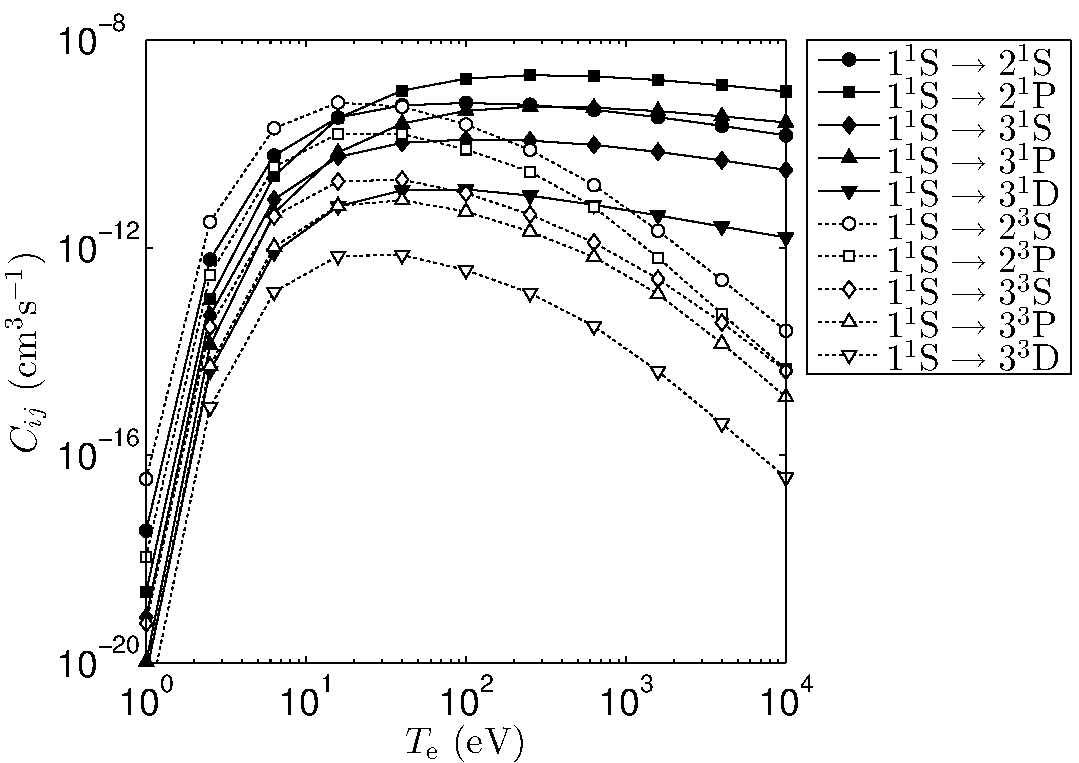
\includegraphics[height=0.35\textheight]{excRate-from-1.pdf}
  \caption{氦原子基态的电子碰撞激发速率系数,计算自 \onlinecite{Ralchenko2008603,NIFS:DATA:059} 的电子碰撞截面数据。}
  \label{fig:chap01:excRate:gs}
\end{figure}

氦原子的能级结构特点决定了其发射光谱适合用来进行托卡马克等离子体的诊断。

首先,氦原子能级结构拥有自旋单重态(singlet)和三重态(triplet)两套电子自旋系统。自旋三重态能级只能通过自旋变化过程激发产生,而自旋单重态能级主要通过自旋守恒过程从基态激发产生,不同自旋系统能级间的电子碰撞跃迁反应截面与相同自旋系统能级间电子碰撞跃迁的反应截面具有不同的随 $T_{\rm e}$ 的变化行为(图 \ref{fig:chap01:excRate:gs}--\ref{fig:chap01:excRate:metasinglet})。对于基态原子,当电子温度高于 $20\,{\rm eV}$ 时,自旋变化和自旋守恒过程的电子碰撞速率系数变化趋势开始有明显的差别(图 \ref{fig:chap01:excRate:gs}),自旋守恒激发过程的速率系数在 $T_{\rm e}$ 为几百电子伏时具有最高值,并且当 $T_{\rm e}$ 在 $50\,{\rm eV}$ 至 $1\,{\rm keV}$ 范围可以视为常数,而自旋变化过程的电子碰撞激发速率系数在 $T_{\rm e}\sim 20\,{\rm eV}$ 时达到最高值,随着 $T_{\rm e}$ 的升高大致按照 $T_{\rm e}^{-2}$ 的速率下降。氦原子亚稳态原子 $2^3{\rm S}$ 和 $2^1{\rm S}$ 的碰撞激发速率系数在图 \ref{fig:chap01:excRate:metatriplet} 和图 \ref{fig:chap01:excRate:metasinglet} 中画出。可见,亚稳态电子碰撞激发速率系数的最高值出现在比基态更低的 $T_{\rm e}$ 处。两亚稳态的自旋守恒激发速率系数分布更为平坦,而自旋变化过程的速率系数在 $T_{\rm e}<10\,{\rm eV}$ 时就开始下降。同时,图 \ref{fig:chap01:excRate:metatriplet} 中画出了 $2^3{\rm S}$ 至 $2^1{\rm S}$ 的电子碰撞跃迁速率系数,它大概是激发至主量子数 $n=3$ 自旋单重态能级速率系数的 $10$ 倍。所以,来自从不同自旋系统能级的谱线强度之比与 $T_{\rm e}$ 有较强的函数关系,而来自相同自旋系统能级的谱线强度比与 $N_{\rm e}$ 具有较强的函数关系,通过测量氦原子谱线辐射可以同时确定等离子体的 $T_{\rm e}$ 和 $N_{\rm e}$ 。

\begin{figure}
  \centering
  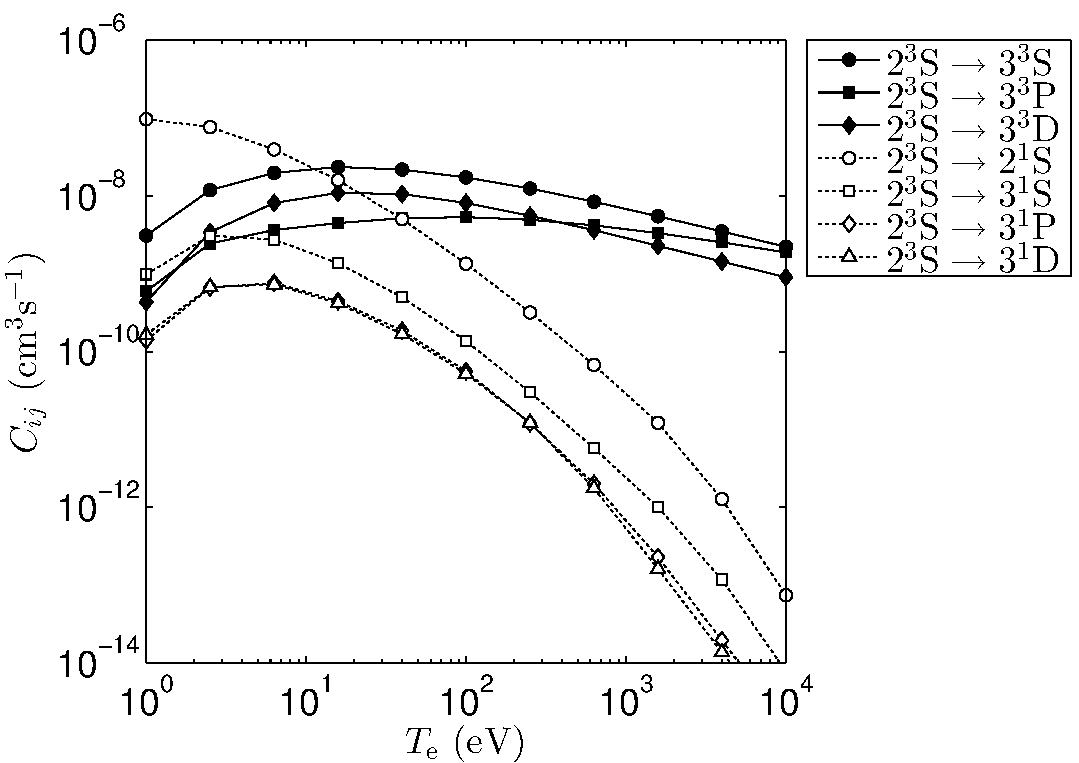
\includegraphics[height=0.35\textheight]{excRate-from-2.pdf}
  \caption{氦原子三重态亚稳态 $2^3{\rm S}$ 的电子碰撞激发速率系数,计算自 \onlinecite{Ralchenko2008603,NIFS:DATA:059} 的电子碰撞截面数据。}
  \label{fig:chap01:excRate:metatriplet}
\end{figure}

其次,在所有原子中,氦原子具有最高的基态电离能 $24.6\,{\rm eV}$。在氦原子束诊断托卡马克等离子体时,诊断束可以达到更深的位置,从而拓宽了诊断范围。

最后,氦为未来聚变等离子体中的固有元素,只需被动地测量氦原子的谱线辐射即可获得等离子体参数信息,不会给等离子体带来新的杂质粒子,即使现阶段大型托卡马克装置中利用氦束进行主动诊断,打入真空室的氦也不会对等离子体本身产生明显的影响\cite{Schmitz2008}。

因此,氦原子的发射光谱诊断(atomic emission spectroscopy)在高温聚变等离子体研究中得到了充分的重视,ITER 装置也已经考虑将氦原子的谱线诊断作为一种重要的诊断手段\cite{Mullane2002}。

\begin{figure}
  \centering
  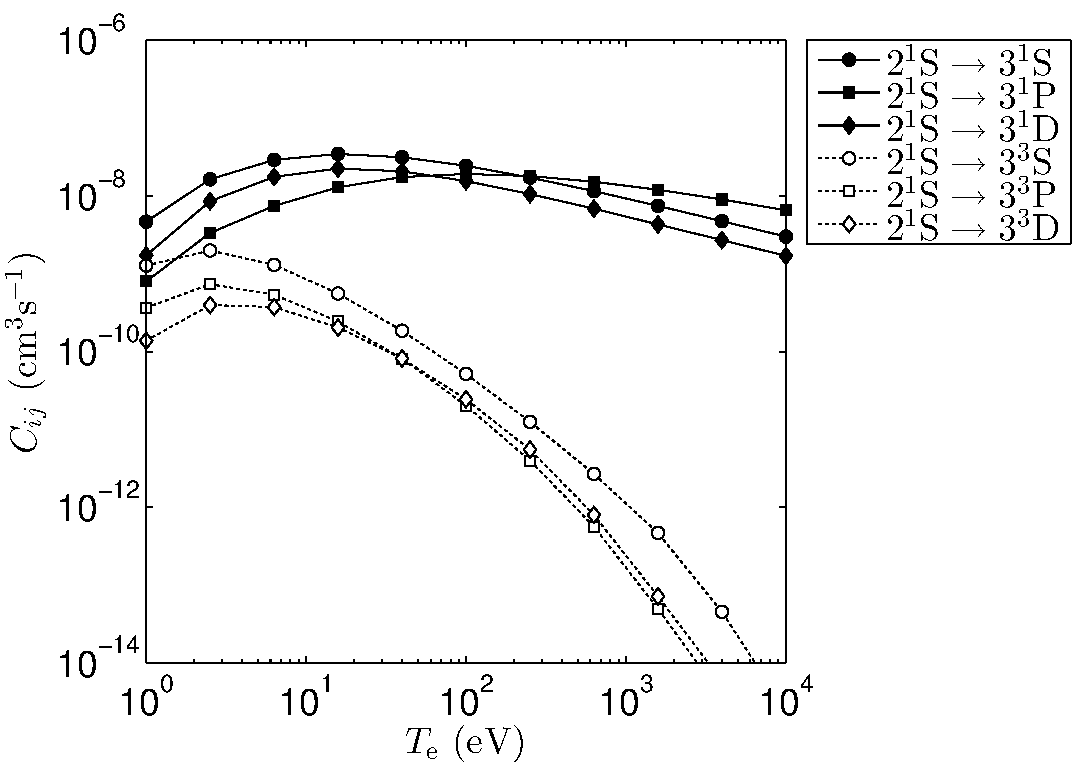
\includegraphics[height=0.35\textheight]{excRate-from-3.pdf}
  \caption{氦原子单重态亚稳态 $2^1{\rm S}$ 的电子碰撞激发速率系数,计算自 \onlinecite{Ralchenko2008603,NIFS:DATA:059} 的电子碰撞截面数据。}
  \label{fig:chap01:excRate:metasinglet}
\end{figure}


\subsection{氦原子发射光谱诊断的研究进展}
\label{sec:chap01:research-history}

最早提出使用自旋单重态和自旋三重态能级谱线辐射强度比方法测量等离子体电子温度的方法时
\cite{Sovie1964-He-coronal,Vries1966-He-coronal},是基于日冕模型(coronal model)的,后来研究中发现此方法只适用于电子密度很低的等离子体, 当 $N_{\rm e}$ 达到 $10^{11}\,{\rm cm}^{-3}$ 以上时,激发态的电子碰撞退激发过程对激发态数密度的影响加剧,此时应该使用碰撞辐射模型(collisional-radiative model)来计算激发态数密度分布\cite{Newe1966-He-CRRecommend}。

人们使用氦束发射光谱(beam emission spectroscopy)诊断等离子体参数是在 TEXTOR\cite{Schweer1992174} 上开始的。后来的类似诊断\cite{Davies1997-HeBES-JET,Field-HeBES-COMPASSD,Hidalgo-HeBES-TJII}
都使用了 TEXTOR 的碰撞辐射模型,该模型中考虑了包括基态在内的主量子数 $n\le 4$ 的共 19 个能级。当氦束为稳态束流时,束流中局域的氦原子激发态数密度保持稳定,只与本地的 $T_{\rm e}$ 和 $N_{\rm e}$ 相关,氦束在等离子体中直线传播,当氦原子被碰撞电离后,即沿磁力线运动而离开束流区域,所以氦离子的复合过程可以忽略,这样用于氦束发射光谱诊断的碰撞辐射模型被大大简化。

后来在 MST 上进行了高速氦束(fast helium beam)发射谱线的诊断研究\cite{Ahn2007-He-BES},并对例如杂质、磁场和离子碰撞等因素对谱线的影响进行了讨论,模型采用了 ADAS\cite{ADAS} 的代码和截面数据,包含了众多能级($n\le 110$),对主量子数能级 $n\le5$ 的能级根据 $nlSL$ 分别处理,将更高能级自旋相同的能级简并。最近 TEXTOR 对模型进行了进一步发展\cite{Schmitz2008},包括了较高的能级粒子,并对重粒子碰撞跃迁和电荷交换过程进行了考虑。而 MAP-II 偏滤器模拟装置\cite{Iida2010-HeBES-MAPII}的束发射光谱诊断工作中使用了 M. Goto 的模型\cite{Goto2003-HeCRM},并对辐射在等离子体中的捕获效应进行了讨论。

\begin{table}
\caption{氦束发射光谱诊断等离子体参数实验及使用的碰撞辐射模型}
{\small nlSL:能级以 nlSL 区分;nS:能级以自旋角动量区分;n:能级仅以主量子数区分;e-He:电子碰撞过程;rad:辐射过程;CX:电荷交换过程;ion-ion/dblion:离子碰撞电离与双电子电离;ion-exc/deexc:离子碰撞激发与退激发;D-tran:氘输运过程;rad-trap:辐射俘获效应。}
\label{tab:chap01:HeBES:CRM}
\begin{center}
\begin{tabular}{llllll}
\toprule[1.5pt]
       装置 & 区域 & 谱线能级 & 包含能级 & 包含过程 & 来源\\
\midrule[1pt]
    TEXTOR & 边界
            & $3^1{\rm D}$, $3^1{\rm S}$, $3^3{\rm S}$
            & $n\le4$
            & e-He, rad
            & \onlinecite{Schweer1992174} \\ \addlinespace[.5em]
    JET & 偏滤器
            & $3^1{\rm D}$, $3^1{\rm S}$, $3^3{\rm S}$
            & $n\le4$
            & e-He, rad
            & \onlinecite{Davies1997-HeBES-JET} \\ \addlinespace[.5em]
  COMPASS-D & 边界
            & $3^1{\rm D}$, $3^1{\rm S}$, $3^3{\rm S}$
            & $n\le4$
            & e-He, rad
            & \onlinecite{Field-HeBES-COMPASSD} \\ \addlinespace[.5em]
      TJ-II & 边界
            & $3^1{\rm D}$, $3^1{\rm S}$, $3^3{\rm S}$
            & $n\le4$
            & e-He, rad
            & \onlinecite{Hidalgo-HeBES-TJII} \\ \addlinespace[.5em]
    MST & 边界
            & $3^1{\rm D}$, $4^1{\rm D}$, $3^1{\rm P}$
            & \makecell[l]{nlSL: $n\le5$,\\
                nS: $6\le n\le 110$}
            & \makecell[l]{e-He, rad, CX\\
                ion-ion/dblion,\\ ion-exc/deexc}
            & \onlinecite{Ahn2007-He-BES} \\ \addlinespace[.5em]
    TEXTOR & 边界
            & $3^1{\rm D}$, $3^1{\rm S}$, $3^3{\rm S}$
            & \makecell[l]{nlSL: $n\le4$,\\
                nS: $5\le n\le 7$,\\
                n: $n=8, 9$, He$^+$}
            & \makecell[l]{e-He, rad, D-CX\\
                D-tran($\Delta n=0$)}
            & \onlinecite{Schmitz2008} \\ \addlinespace[.5em]
    MAP-II & \makecell[l]{偏滤器\\ 模拟装置}
            & \makecell[l]{$3^1{\rm D}$, $3^1{\rm P}$\\
                $4^3{\rm S}$, $3^3{\rm D}$, $3^3{\rm S}$}
            & 与 \onlinecite{Goto2003-HeCRM} 相同
            & \onlinecite{Goto2003-HeCRM}, rad-trap
            & \onlinecite{Iida2010-HeBES-MAPII} \\
\bottomrule[1.5pt]
\end{tabular}
\end{center}
\end{table}

表 \ref{tab:chap01:HeBES:CRM} 列出了用氦束发射光谱作为等离子体诊断手段的一些实验,这些实验主要集中在对边界和偏滤器等离子体的诊断,氦束发射光谱诊断法可以获得很高空间分辨率的 $T_{\rm e}$ 和 $N_{\rm e}$ 参数,对托卡马克等离子体的粒子输运、L--H 转换,MHD 约束行为的研究有很重要的作用。

在氦束发射光谱诊断的碰撞辐射模型处理上,氦原子被电离后便沿磁力线运动离开束流区域,在模型中则一般忽略氦离子对能级数密度的贡献。但是,在氦(或混入氦气)等离子体中,氦离子的影响则不再可以忽略,T. Fujimoto\cite{Fujimoto1979-HeCR} 建立了适用于低温氦气放电等离子体($N_{\rm e}=6.3\times10^{10}\,{\rm cm}^{-3}$, $T_{\rm e}=6\,{\rm eV}$)的碰撞辐射模型。在每种不同的等离子体条件下,添加不同的过程或外界条件的影响,T. Fujimoto 的模型在实验中得到了充分的应用和验证。同时,M. Goto 分别在 1997\cite{Goto1997-HeCRM-WT3} 和2003\cite{Goto2003-HeCRM} 年根据最新的碰撞截面数据对此模型进行了修订和更新。基于此模型在一些等离子体中的诊断应用总结于表 \ref{tab:chap01:FujimotoHeCRM:applications} 中。

\begin{table}
\caption{T. Fujimoto 的碰撞辐射模型在不同等离子体条件下的应用}
{\small wall: 器壁猝熄过程(quenching at wall);meta-meta:亚稳态原子非线性碰撞过程;$\nu$-abs/exc/ion:辐射吸收、激发与电离过程;hot-e:射频加热产生的热电子效应;res-scat:辐射的共振散射效应(resonance scattering of radiation);ionizing condition: 激发态粒子数密度独立于 ${\rm He}^+$ 密度。}
%\vspace{-1.5em}
\label{tab:chap01:FujimotoHeCRM:applications}
\begin{center}
\begin{tabular}{llll}
\toprule[1.5pt]
       装置 & 等离子体条件 & 添加过程或实验技术 & 来源\\
\midrule[1pt]
     - & 辉光放电
            & \makecell[l]{wall, meta-meta,\\ $\nu$-abs/exc/ion}
            & \onlinecite{Fujimoto1979-HeCR} \\ \addlinespace[.5em]
   NAGDIS-I & 氦等离子体
            & \makecell[l]{hot-e, res-scat}
            & \onlinecite{Sasaki1996-HeCRM-NAGDIS} \\ \addlinespace[.5em]
   JT-60U & \makecell[l]{偏滤器再循环氦}
            & \makecell[l]{ionizing condition}
            & \onlinecite{Hirotaka1999-HeCRM-JT60U} \\ \addlinespace[.5em]
   WT-3 & \makecell[l]{10\% 混氦}
            & \makecell[l]{$L-S$ 耦合}
            & \onlinecite{Goto1997-HeCRM-WT3} \\ \addlinespace[.5em]
   LHD & \makecell[l]{混氦}
            & \makecell[l]{$L-S$ 耦合}
            & \onlinecite{Goto2003-HeCRM} \\ \addlinespace[.5em]
  HYBTOK-II & \makecell[l]{氦等离子体}
            & \makecell[l]{CCD 相机 2 维测量}
            & \onlinecite{Ohno2010-HeCRM-2D-measure} \\
  H-1 & \makecell[l]{混氦}
            & \makecell[l]{计算机断层重建}
            & \onlinecite{MaShuiliang2012:Tomography} \\
\bottomrule[1.5pt]
\end{tabular}
\end{center}
\end{table}

从谱线强度比数据中分析出等离子体 $T_{\rm e}$ 和 $N_{\rm e}$ 的过程以碰撞辐射模型对等离子体谱线强度比与$T_{\rm e}$ 和 $N_{\rm e}$ 之间关系的计算为基础
\cite{Fujimoto1979-HeCR,Goto2003-HeCRM,boivin2001},碰撞辐射模型的建立包括选取模型包含的激发态能级,对能级之间电子碰撞反应过程的处理以及这些反应过程的速率系数(反应截面)的计算,在实际工作中,这些因素都会对模型的计算结果产生影响。早期的工作中\cite{Fujimoto1979-HeCR},人们期待在碰撞辐射模型中加入足够多的反应能级和碰撞辐射过程来满足计算结果的有效性,但由于包含的激发态能级不同,以及使用的速率系数精度较低\cite{Summers:IAEAdatarequirement},不同模型的计算结果差别较大
\cite{Boivin2007}。后来,M. Goto\cite{Goto2003-HeCRM}尝试更新模型的反应速率系数以获得精度更高的计算结果,同时 Y. Andrew 等人\cite{Andrew2000PPCFSensitivity}计算了模型中反应速率系数的不确定度对计算结果的影响,在 O. Schmitz 等人\cite{Schmitz2008}的工作中,将氦谱线比的诊断结果与其他诊断手段的结果进行对比来验证谱线比法诊断结果的有效性。

\begin{figure}%[H]
  \centering
  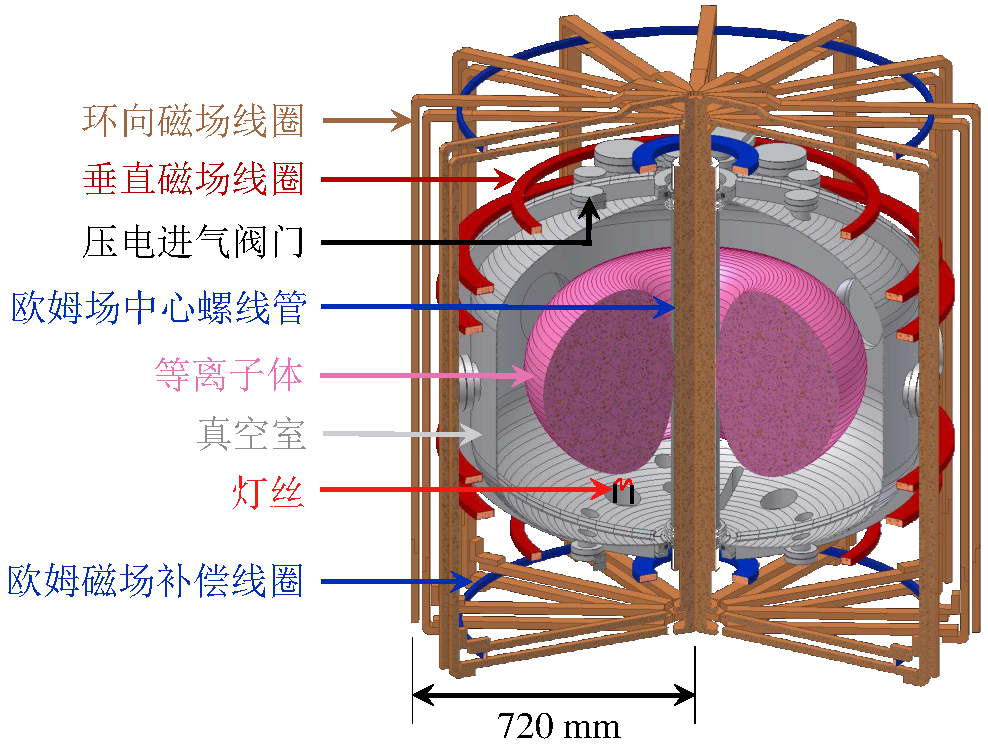
\includegraphics[width=0.8\textwidth]{SUNIST-Sketch-14_cropped.pdf}
  \caption{SUNIST 装置示意图,修改自\onlinecite{sunist:sketch:wiki}}
  \label{fig:chap01:sunist-sketch}
\end{figure}

%\subsection{国内研究现状}
\subsection{国内托卡马克等离子体的光谱诊断研究}

国内的托卡马克研究者也进行了大量的光谱诊断工作。在 CT-6B 装置中,李赞良等人\cite{LiZanliang:CT-6B:Te} 在 1989 年通过氧离子的真空紫外光谱测量了电流上升阶段的电子温度;后来赵庆勋等人\cite{ZhaoQingxun:CT-6B:Rotate}在 1997 年根据 OII $464.2\,{\rm nm}$、CIII $464.7\,{\rm nm}$ 和 ${\rm H}_\alpha$ 谱线的多普勒位移,测量了等离子体极向转动速度的径向分布。在 HT-7 装置上,刘建坤\cite{LiuJiankun2001:HT-7:PDA}等人使用光电二极管阵列,测量了 ${\rm H}_\alpha/{\rm D}_\alpha$ 的光谱,对粒子约束时间进行了系统研究;周倩等人\cite{ZhouQian2005:HT-7:carbon}在 2005 年通过对碳杂质的谱线辐射进行空间分辨测量,研究了碳杂质在径向的输运行为并在 2007 年完善了用于轻杂质粒子输运研究的光谱诊断系统;2010 年 HT-7 上用于电荷交换复合光谱诊断的诊断中心束束系统建成,实现了离子温度剖面分布测量\cite{ShiYuejiang2010:HT-7:CXRS};同时,陈开云等人\cite{ChenKaiyun2009:HT-7:SXTomography} 在 HT-7 上开展了基于断层扫描技术的软 X 射线诊断工作。在 J-TEXT 装置上通过测量软 X 射线辐射进行了反锯齿行为(inverse sawtooth activity)的研究\cite{FengXD2013:J-TEXT:softxray}。 崔正英等人\cite{CuiZhengying:2010:VUV}在 HL-2A 装置上建立了具有空间分辨诊断能力的真空紫外光谱测量系统,可以用于边界杂质和温度分布的测量。在 EAST 装置上,新建立了充气成像系统(gas puffing imaging),此系统可以有效的测量等离子体边界的湍流结构\cite{LiuSC:2012:EASTGPI},利用此系统成功研究了 L--H 转换的中间振荡过程(intermediate oscillatory phase)\cite{XuGS2014:EASTGPI:L-I-H}。

由此可见,虽然国内托卡马克光谱诊断研究众多,但基于碰撞辐射模型,通过测量原子谱线辐射强度比的方法诊断 $T_{\rm e}$ 和 $N_{\rm e}$ 参数的研究在国内尚未见报道。而低温等离子体研究领域,国内的研究者对此进行了大量有意义的研究工作\cite{ZhuXM2010:Review}。通过低温等离子体可见光谱辐射诊断的研究\cite{ZhuXM2009:Thesis} 发现,根据等离子体条件做必要的假设,通过在碰撞辐射模型中包含最主要的粒子和过程,可以对谱线比法诊断等离子体进行有效的指导。

\subsection{SUNIST 装置、等离子体参数范围与诊断需求}

\begin{figure}%[H]
  \centering
  \begin{overpic}[width=0.6\textwidth]{sunist_parram_vs_lineratio_range_2.pdf}
    \put(45,34){氦谱线比法}
	\put(51,45){SUNIST}
  \end{overpic}
  %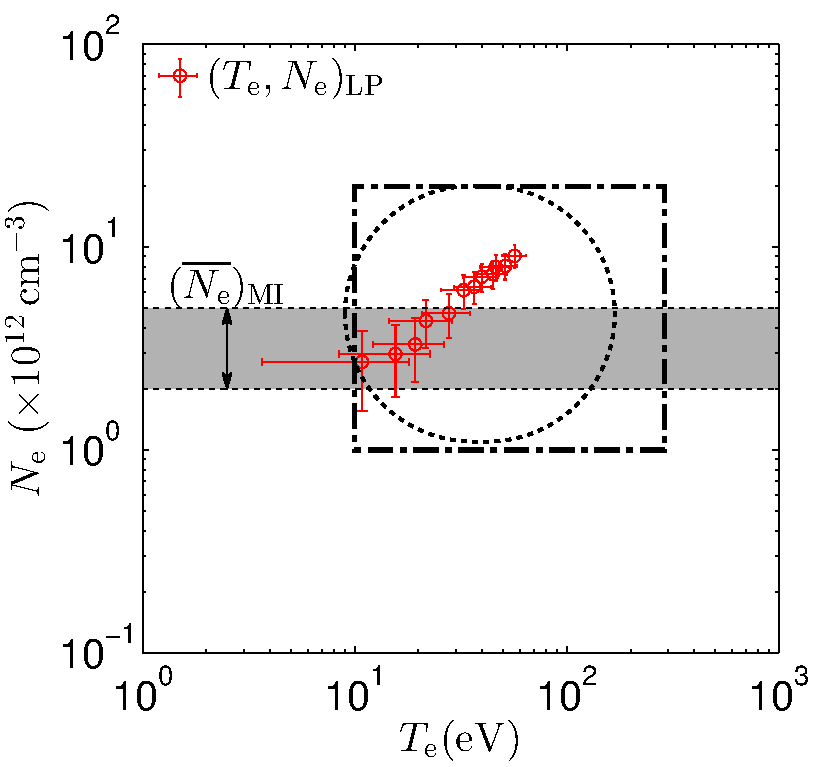
\includegraphics[width=0.6\textwidth]{sunist_parram_vs_lineratio_range_2.pdf}
  \caption{氦谱线比法诊断适用的电子参数范围与 SUNIST 等离子体参数范围估计。$(T_{\rm e},N_{\rm e})_{\rm LP}$ 表示静电探针测量的 SUNIST 边界等离子体参数\cite{WangWH2005:PPCF:Edge};$(\overline{N_{\rm e}})_{\rm MI}$ 表示微波干涉仪测量的电子密度范围值(第 \ref{sec:chap04:lineratio-ne-te} 节)。点划线表示氦原子谱线比法的适用范围;点线表示 SUNIST 等离子体电子参数估计范围。}
  \label{fig:chap01:te-ne-range}
\end{figure}

中国联合球形托卡马克(Sino-UNIted Spherical Tokamak,SUNIST)是我国第一台,也是唯一一台球形托卡马克装置\cite{Heyexi2002:SUNIST},图 \ref{fig:chap01:sunist-sketch} 所示为 SUNIST 装置示意图。

SUNIST 装置的主要参数为:大半径 $R_0=0.3\,{\rm m}$,小半径 $a=0.23\,{\rm m}$,欧姆放电时的等离子体电流 $I_{\rm p}\sim50\,{\rm kA}$,边界电子温度 $T_{\rm e}=20\,{\rm eV}\sim100\,{\rm eV}$ 和电子密度 $N_{\rm e}=1\times10^{12}\,{\rm cm}^{-3}\sim10\times10^{12}\,{\rm cm}^{-3}$\cite{WangWH2005:PPCF:Edge}(SUNIST 放电时的电子参数范围估计如图 \ref{fig:chap01:te-ne-range} 所示),真空室本底气压$p_{\rm gas,b}\sim5\times10^{-5}\,{\rm Pa}$,氦气放电充气气压范围 $p_{\rm gas}=2\times10^{-3}\,{\rm Pa}\sim5\times10^{-3}\,{\rm Pa}$。

%SUNIST 实验中,传统的等离子体电子参数诊断手段也面临着挑战,如静电探针会被高温等离子体烧蚀(图 \ref{fig:chap01:ProbeVapor}),这不但会缩短静电探针的使用寿命,而且会为诊断数据解析带来困难,烧蚀释放的重元素杂质粒子也会污染等离子体;同时,
SUNIST 做为小型球形托卡马克实验装置,研究人员匮乏,所以 SUNIST 装置亟需部署低成本、不干扰等离子体、少维护或免维护的可靠诊断手段。

%\begin{figure}%[H]
%  \centering
%  %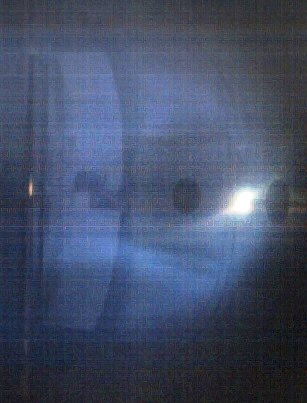
\includegraphics[height=0.3\textheight]{ProbeVapor121123020.jpg}
%  \begin{overpic}[scale=0.7]{ProbeVapor121123020-bw.jpg}
%    \put(1,22){\color{white}{\bf 中心柱}}
%    \put(2,29){\color{white}{$\uparrow$}}
%
%    \put(25,87){\color{white}{\bf 等离子体}}
%    \put(35,80){\color{white}{$\downarrow$}}
%
%    \put(50,59){\color{white}{\bf 静电探针}}
%    \put(67,53){\color{white}{$\downarrow$}}
%
%    \put(50,33){\color{white}{\bf 烧蚀亮点}}
%    \put(58,40){\color{white}{$\uparrow$}}
%  \end{overpic}
%  \caption{SUNIST放电时静电探针烧蚀情况(炮号:121123020)}
%  \label{fig:chap01:ProbeVapor}
%\end{figure}

\subsection{课题意义}
\label{sec:ketiyiyi}

利用等离子体的谱线辐射强度比进行诊断的方法具有不干扰等离子体,光谱测量设备简单且不受复杂电磁环境的影响以及仅需进行相对标定的优点。作为聚变产物,氦在未来聚变堆中是一种固有元素,所以利用氦原子谱线辐射强度比进行电子参数诊断不会为等离子体带入新的杂质,在高温聚变等离子体研究中得到了充分的重视。

然而,根据氦原子的谱线强度分析出 $T_{\rm e}$ 和 $N_{\rm e}$ 是以碰撞辐射模型对氦原子激发态数密度的计算为基础的。原子反应速率系数和碰撞辐射模型中包含的能级以及反应过程是影响碰撞辐射模型计算精度的主要因素。
%现阶段原子反应速率系数(或截面)数据主要有以下三种来源:实验测量
%\cite{Shah1988:ionizaiton-data-measure,Long1970:PhysRevA.1.260,Dixon1976}、
%理论计算\cite{CCCmethod,Sawey199381}与半经验公式拟合\cite{Fujimoto:IPPJ-AM-8},并且有人对此专门做过总结
%\cite{IAEA:Data:vol3,deHeer:INDC,Kato:NIFS:DATA:346}。然而这些数据来源的精度难以保证\cite{Ralchenko2008603},导致不同来源原子反应数据的碰撞辐射其计算结果也不尽相同\cite{Delabie2010:consistency}。%如第 \ref{sec:chap01:research-history} 节所述,
%为了得到更高精度的计算结果,人们往往在碰撞辐射模型中加入更多的能级粒子、反应过程以及可以对原子能级产生影响的因素。但因为使用的截面数据精度不一,导致碰撞辐射模型中包含更多的能级和反应过程时,并不能如预期那样获得更高精度的计算结果(第 \ref{sec:chap02:crm-problem} 节)。
%而且,
碰撞辐射模型中包含着众多的能级粒子和复杂的反应过程,且相互耦合,现并无有效的手段对碰撞截面数据不确定性到粒子数计算误差的传递进行有效计算的手段,也就无法对不同原子反应过程的数据提出具体的精度要求。
随着原子能级的升高,其原子数密度快速下降,在碰撞辐射模型中的重要性也随之下降。随之带来的问题是,在特定的等离子体参数条件下,碰撞辐射模型中包含至多高能级的激发态能级才能满足光谱诊断研究对精度的要求。
%或者由碰撞辐射模型中包含粒子数精简带来的误差会小于由原子反应速率系数精度的限制所带来的误差。

以上问题在托卡马克等离子体氦原子谱线比诊断的文献中鲜有报道。在低温等离子体研究领域,人们意识到这个问题\cite{ZhuXM2009:Thesis},并尝试在碰撞辐射模型中只包含与感兴趣能级粒子相关的主要过程,通过与实验的对比,来验证碰撞辐射模型的有效性。

在高温等离子体氦发射光谱诊断等离子体参数的实验中,适用的等离子体参数范围\cite{Schmitz2008} 为:$20\,{\rm eV}<T_{\rm e}<300\,{\rm eV}$ 与 $10^{12}\,{\rm cm}^{-3}<N_{\rm e}<2\times10^{12}\,{\rm cm}^{-3}$,这与 SUNIST 整个等离子体区域的参数范围一致(如图 \ref{fig:chap01:te-ne-range} 所示)。做为一台小型托卡马克装置,SUNIST 具有实验安排灵活的优势,适合进行诊断原理的验证性研究。
因此,我们在 SUNIST 中开展了氦原子光谱诊断研究。本文将根据 SUNIST 氦放电等离子体的特点建立碰撞辐射模型,研究影响模型计算结果的因素,包括速率系数不确定性和碰撞辐射模型中包含的能级粒子的影响等;验证利用氦原子谱线辐射强度比诊断 SUNIST 等离子体参数物理和技术上的可行性;并且在研究工作中为 SUNIST 完善运行设施,建立起光谱诊断系统,积累光谱诊断经验;同时,也希望为其他托卡马克装置采用此诊断提供参考。%奠定基础。

\section{本文研究思路、内容和结构}

\begin{figure}%[H]
  \centering
  
\includegraphics[width=0.8\textwidth]{research-progress.pdf}
  \caption{本论文研究过程图}
  \label{fig:chap01:research-progress}
\end{figure}

本文以氦放电等离子体的原子发射光谱诊断 $T_{\rm e}$ 和 $N_{\rm e}$ 为对象,完成了碰撞辐射模型的建立、实验系统建设、诊断方法的建立和验证等研究内容。图 \ref{fig:chap01:research-progress} 和图 \ref{fig:chap01:research-relationship} 分别显示的是本论文研究过程图和各部分研究内容之间的关系。

论文首先建立适用于 SUNIST 氦放电等离子体的碰撞辐射模型,然后根据模型对谱线比的预测与实验测量进行对比得到等离子体的 $T_{\rm e}$ 和 $N_{\rm e}$ 参数,最后验证该方法的有效性,并针对影响诊断结果的因素进行讨论。

在碰撞辐射模型方面,首先分析了 SUNIST 等离子体参数下的氦原子激发态数密度分布特点,选定模型粒子数密度方程中包含的激发态能级和反应过程,并选择合适的反应截面数据进行计算。该部分是光谱诊断的基础,为从谱线强度测量数据获得相应等离子体参数提供谱线强度比预测结果。

碰撞辐射模型在特定的等离子体参数空间提供了原子谱线强度比的预测结果,而通过实验数据获得对应参数则是一个反过程。为了获得实验数据,课题工作中建立了相应的光谱诊断设备,对单色仪各项参数进行了标定,并尽最大限度对光电倍增管的信号信号和干扰做了消除减弱。%首先需要对 SUNIST 的放电控制进行优化。同时需要建立起相应的实验测量设备,包括实验数据采集以及光谱诊断设备等。

对发射光谱法诊断手段的验证内容手段有:在诊断得到的等离子体参数下,模型计算的激发态能级数密度和实验测量对比对碰撞辐射模型的复核;影响模型对谱线比预测结果的因素\pozhehao 包括能级的选取、速率系数的不确定性等\pozhehao 的分析;以及光谱测量的弦积分特性带来的误差的分析等。

%论文各部分内容的关系如下(图 \ref{fig:chap01:research-relationship}):1)在给定的等离子体参数空间内,利用碰撞辐射模型给出的粒子数方程计算出谱线比方法感兴趣能级的数密度;2)将有效自发辐射跃迁速率系数与能级数密度相乘,得到氦原子谱线强度,进而计算出谱线强度比在等离子体参数空间的分布;3)把实验测得的谱线数据与光谱仪响应的标定结果相结合,得到实验测量的谱线强度比;4)将碰撞辐射模型计算与实验测量的谱线强度比进行对比,得到等离子体的具体 $T_{\rm e}$ 与 $N_{\rm e}$ 参数;5)在获得的 $T_{\rm e}$ 与 $N_{\rm e}$ 参数下,可以用碰撞辐射模型计算出所有实验中测量的谱线激发态能级的数密度,将其与实验测量数据计算得到的激发态数密度进行对比,复核碰撞辐射模型对等离子体中的碰撞与辐射过程描述。

通过氦原子谱线辐射诊断 $T_{\rm e}$ 和 $N_{\rm e}$ 的工作,本文建立了从模型建立到实验测量,再到数据分析以及对诊断结果进行评估的整体框架。

\begin{figure}%[H]
  \centering
  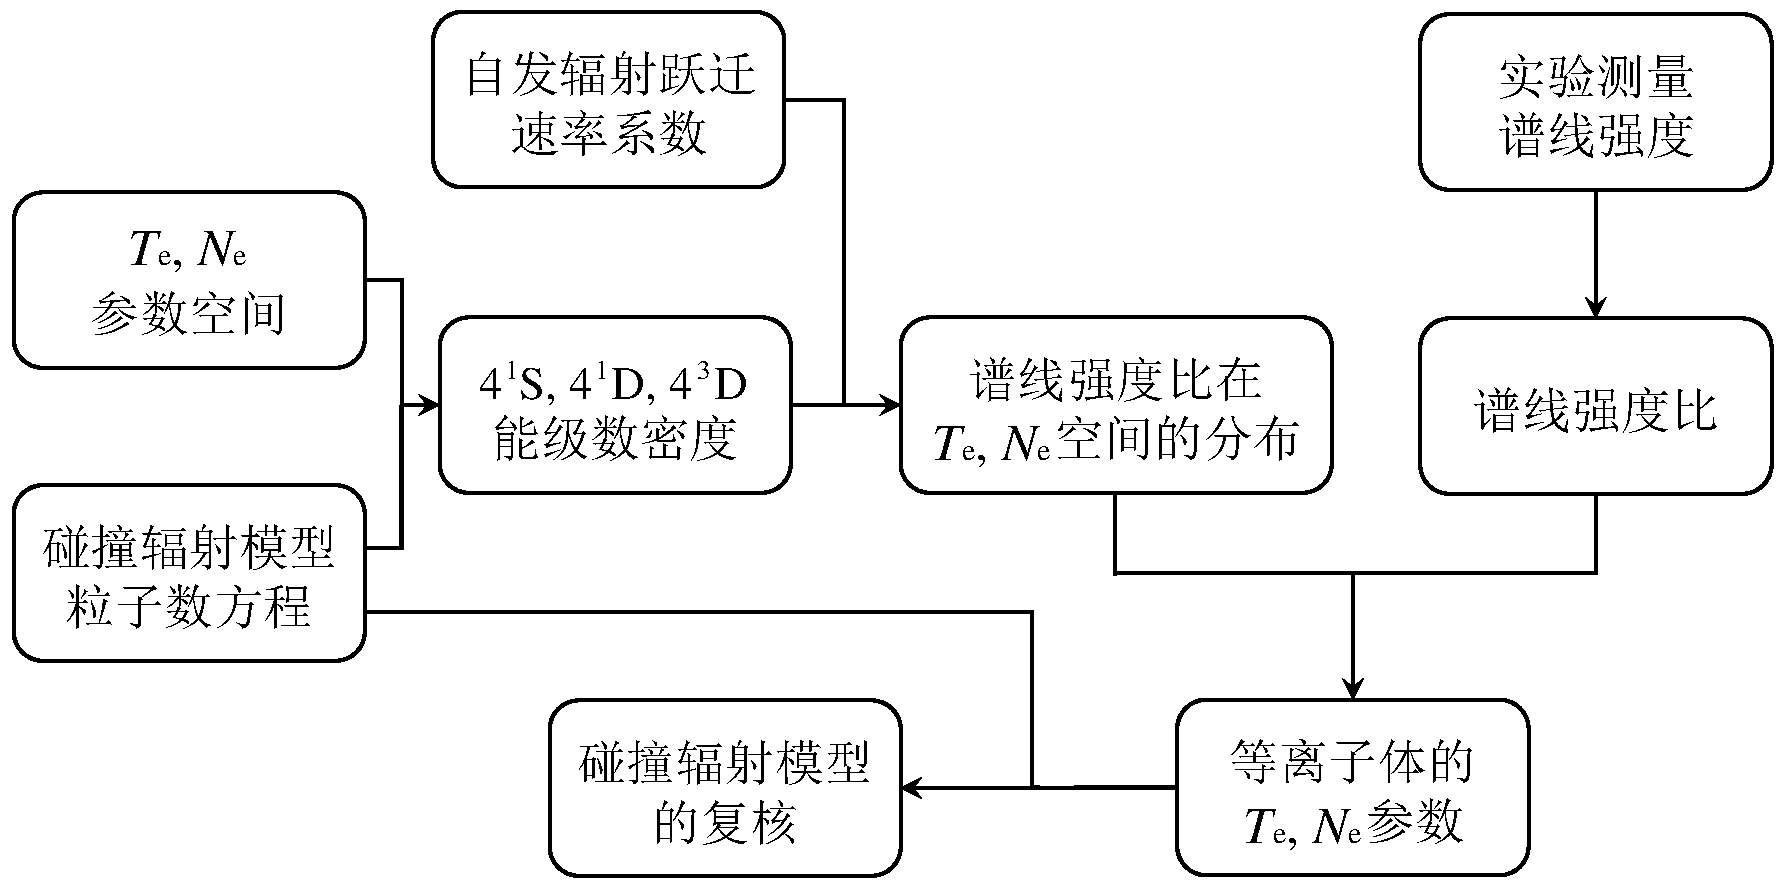
\includegraphics[width=\textwidth]{lineratio-method-rellevelabun.pdf}
  \caption{各部分研究内容的关系}
  \label{fig:chap01:research-relationship}
\end{figure}

本文结构如下:

第 \ref{chap:introduction} 章阐述了托卡马克高温聚变等离子体中光谱发射诊断研究的概况,介绍了本文研究的意义,给出了论文的主要研究内容和安排。

第 \ref{chap:crm-intro} 章从光子产生至被光谱系统检测测量所经历的物理过程出发,分析了影响谱线强度的因素:自发辐射跃迁几率、光子在等离子体内的传输以及自发辐射跃迁上能级激发态粒子数密度。给出了日冕、碰撞辐射模型和局域热平衡三种主要描述等离子体内粒子数密度分布的模型。介绍了高温聚变等离子体研究中使用的碰撞辐射模型的一般处理方法,并在最后指出现阶段氦原子谱线比诊断研究中使用的碰撞辐射模型所存在的一些问题,即反应速率系数不确定性至激发态数密度的传递估计手段不明确,以及模型中应包含的粒子和反应过程缺乏系统研究。

第 \ref{chap:crmodel} 章通过分析 SUNIST 氦放电等离子体内氦原子的特点(如原子能级数密度分布特点、等离子体的光学厚度、杂质影响和多种过程的时间常数等)建立了相应的碰撞辐射模型。通过选取使用前人整理的碰撞反应截面数据,求解了模型结果并与 FLYCHK 代码包的计算结果进行对比。最后,根据 SUNIST 氦放点等离子体的实验测量选取合适的谱线比,建立了氦原子谱线比诊断电子温度和密度的方法。

第 \ref{chap:measureing-system} 章介绍了 SUNIST 上的光谱诊断系统,包括光谱测量系统和测量路径安排,单色仪的谱线准确性、分辨率以及测量系统光谱响应的标定结果等。同时,介绍了降低信号噪声和消除基线干扰的手段,给出了 SUNIST 上基于重复放电的光谱测量手段以及氦原子谱线测量结果。相同的控制条件下 SUNIST 放电重复性的保证是测量的前提,本章也介绍了对提高放电重复性所做的研究,通过设计和安装 SUNIST 进气系统,改善了 SUNIST 放电的重复性。

第 \ref{chap:experiment} 章给出了 SUNIST 氦放电等离子体的光谱测量和等离子体电子温度与密度的诊断结果。通过其他未使用谱线对应激发态能级粒子数密度与碰撞辐射模型计算结果的对比,复核了本文建立的碰撞辐射模型。研究中还观察到弦积分光谱测量诊断的电子密度与微波干涉仪测量的弦平均电子密度的比值与电子参数剖面分布的峰化与否有直接关系、原子谱线强度与磁探针信号具有相同的涨落行为等结果,这为今后丰富和深入光谱诊断研究内容提供了参考和指引。

第 \ref{chap:summary} 章对本课题研究工作进行总结,指出工作的不足之处,并对未来的光谱诊断研究工作进行展望。


\graphicspath{{figures/chap02/}}

%\chapter{等离子体原子发射谱线与碰撞辐射模型}
\chapter{原子谱线强度比诊断等离子体电子温度与密度概述}
\label{chap:crm-intro}

不同元素原子的能级结构是不相同的,具有不同的光谱辐射。通过对原子发射光谱的测量和分析,不仅可以定性地分析气体成分,还可以定量地分析各种元素的含量。根据不同原子受激发以及发射光谱的难易程度还可以进行等离子参数的诊断测量,例如电子温度 $T_{\rm e}$ 和电子密度 $N_{\rm e}$。

\section{原子谱线强度比诊断电子温度与密度}

原子受到激发后,由高能级 $j$ 跃迁到低能级 $i$ 时,将辐射出一定能量的光子,光子的波长 $\lambda_{ji}$ 由能级间的能量差 $\Delta E$ 决定:
\begin{equation}
  \lambda_{ji} = \frac{h{\rm c}}{\Delta E}
\end{equation}
式中,$h$ 为普朗克常数(Planck Constant),${\rm c}$ 为光速。其光子数辐射率可以写为\cite{Wiese1966:book}:
\begin{equation}
  %\label{}
  \epsilon_{ji}=\frac{1}{4\pi}N_{j}A_{ji}
\end{equation}
其中,$N_j$ 为跃迁上能级 $j$ 的粒子数密度,$A_{ji}$ 为自发辐射跃迁速率系数(爱因斯坦系数)。

假设均匀等离子体条件下,光谱测量系统获得的光子辐射计数率 $I_{\lambda_{ji}}$ 为:
\begin{equation}
  I_{\lambda_{ji}}=\epsilon_{ji}V\Omega T_{\lambda_{ji}}\eta_{\lambda_{ji}}
\end{equation}
其中,$V$ 为光谱仪可观测到的等离子体体积,$\Omega$ 为光谱接收设备所呈的立体角,$T_{\lambda_{ji}}$ 为等离子体的透射率,$\eta_{\lambda_{ji}}$ 为光学探测系统的量子效率。如果同时测量另外一条波长为 $\lambda_{qp}$ 的谱线,则两条谱线的强度比:
\begin{equation}
\label{eq:chap02:line-ratio}
  \frac{I_{\lambda_{ji}}}{I_{\lambda_{qp}}}=
  \frac{\epsilon_{ji}T_{\lambda_{ji}}\eta_{\lambda_{ji}}}{\epsilon_{qp}T_{\lambda_{qp}}\eta_{\lambda_{qp}}}
  =\frac{1}{F_R}\frac{T_{\lambda_{ji}}N_jA_{ji}}{T_{\lambda_{qp}}N_qA_{qp}}
\end{equation}
其中,$F_R$ 为与仪器响应相关的系数,实验中可以进行标定;自发辐射跃迁速率系数可以通过理论计算获得精确的数值,且一般不受等离子体参数的影响(第 \ref{sec:chap02:Aji} 节)。而由于跃迁上能级的粒子数密度 $N_{j}$ 与 $N_{q}$ 随电子温度与密度具有不同的变化趋势,这样通过建立反映原子反应过程的模型,事先计算出谱线比(式 \ref{eq:chap02:line-ratio})随等离子体电子温度与密度的变化趋势,在实验中测量出对应谱线的强度比,即可以根据模型计算结果反推出等离子体的电子温度和密度。

以 Z 箍缩氖等离子体中氖原子的 $K$ 壳层谱线辐射为例\cite{LiJing:WLXB},通过建立描述原子反应过程的碰撞辐射模型,计算出 ${\rm H}_\alpha$ 和 ${\rm I.C.}$ 谱线分别与 ${\rm He}_\alpha$ 谱线的强度比在电子温度--电子密度空间内的分布,其等高线如图 \ref{fig:chap02:lijing-a} 与 \ref{fig:chap02:lijing-b} 所示,其中谱线强度比 ${\rm H}_\alpha/{\rm He}_\alpha$ 主要与电子温度相关,谱线强度比 ${\rm I.C.}/{\rm He}_\alpha$ 主要与电子密度相关。如果在实验中同时测量该两谱线强度比值分别为 $0.53$ 与 $0.15$ 时,即可以同时确定等离子体的电子温度与密度参数,如图 \ref{fig:chap02:lijing-c} 所示。

\begin{figure}%[H]
  \centering
  \begin{subfigure}{0.45\textwidth}
  \begin{overpic}[width=\textwidth]{lijing-a.pdf}
    \put(15,63.5){\mbox{\colorbox{white}{\small\hspace{1em}}}}
    %\put(-2,30){\rotatebox{90}{\mbox{\colorbox{white}{\small\hspace{2em}激发截面 (${\rm m}^2$)\hspace{2em}}}}}
  \end{overpic}
  \caption{谱线强度比 ${\rm H}_\alpha/{\rm He}_\alpha$ 等高线}
  \label{fig:chap02:lijing-a}
  \end{subfigure}
  \hspace{0.03\textwidth}
  \begin{subfigure}{0.45\textwidth}
  \begin{overpic}[width=\textwidth]{lijing-b.pdf}
    \put(86,65){\mbox{\colorbox{white}{\hspace{0.5em}}}}
    %\put(-2,25){\rotatebox{90}{\mbox{\colorbox{white}{\small\hspace{2em}激发速率系数 (${\rm m}^3/{\rm s}$)\hspace{2em}}}}}
  \end{overpic}
  \caption{谱线强度比 ${\rm I.C.}/{\rm He}_\alpha$ 等高线}
  \label{fig:chap02:lijing-b}
  \end{subfigure}
  \\%\hspace{0.03\textwidth}
  \begin{subfigure}{0.45\textwidth}
  \begin{overpic}[width=\textwidth]{lijing-c.pdf}
    %\put(30,0){\mbox{\colorbox{white}{\small\hspace{2em}$T_{\rm e} (${\rm eV}$)$\hspace{2em}}}}
    %\put(-2,25){\rotatebox{90}{\mbox{\colorbox{white}{\small\hspace{2em}激发速率系数 (${\rm m}^3/{\rm s}$)\hspace{2em}}}}}
  \end{overpic}
  \caption{同时确定电子温度和密度的关系曲线}
  \label{fig:chap02:lijing-c}
  \end{subfigure}
  \caption{Z 箍缩氖等离子体中氖 $K$ 壳层的 ${\rm H}_\alpha$ 和 ${\rm I.C.}$ 与 ${\rm He}_\alpha$ 谱线的强度比的模型计算等高线(图 \ref{fig:chap02:lijing-a} 与 \ref{fig:chap02:lijing-b})与两谱线强度比分别为 $0.53$ 和 $0.15$ 时同时确定电子温度与密度的关系曲线(图 \ref{fig:chap02:lijing-c})。图片来自 \onlinecite{LiJing:WLXB}。}
  \label{fig:chap02:lijing}
\end{figure}

%\section{原子发射谱线}
\section{影响原子发射谱线强度的过程}

理论上要计算有多少光子辐射出等离子体区域,需要对以下三个过程进行分析:1)原子激发态自发辐射跃迁几率;2)特定的等离子体条件下原子激发态数密度;3)光子在等离子体中的传播。

\subsection{自发辐射跃迁几率}
\label{sec:chap02:Aji}

自发辐射跃迁几率可以通过原子物理相关理论计算获得,不同的等离子体环境(如温度、密度等)会对原子状态产生影响,但一般来讲等离子体环境对原子激发态自发辐射跃迁几率的影响微乎其微,可以忽略。$j\to i$ 自发辐射跃迁速率系数 $A_{ji}$ 可以由以下方程给出\cite{Kolb1964:A-formular}:
\begin{equation}
  A_{ji}=4.3\times10^7\frac{g_i}{g_j}f_{ij}\Delta E_{ji}^2\,{\rm s}^{-1}
\end{equation}
其中,$g_i$、$g_j$ 和 $\Delta E_{ji}$ 分别为 $i$、$j$ 能级的统计权重和两能级能量差,$f_{ij}$ 为 $i$ 到 $j$ 能级的吸收振子强度(absorption oscillator strength)\cite{Johnson1972:collisionalstrength}。另外,自发辐射跃迁系数也可以在数据库\cite{NISTdatabase}中直接查询获得。

\subsection{描述原子激发态数密度分布的模型}

%现阶段,爱因斯坦系数可以精确获得。而
式 (\ref{eq:chap02:line-ratio}) 中上能级的粒子数 $N_j$ 与 $N_q$ 与等离子体电子温度 $T_{\rm e}$ 和 $N_{\rm e}$ 相关。通过建立原子反应过程模型,事先计算等离子体辐射谱线上能级的粒子数密度与 $T_{\rm e}$ 和 $N_{\rm e}$ 的关系,则可通过测量谱线的强度比反推等离子体的电子温度和密度。

在特定的 $T_{\rm e}$ 和 $N_{\rm e}$ 参数下,通过对等离子体内影响特定原子激发态数密度的反应过程进行研究,以确定此激发态的数密度。这些原子反应过程一般为\cite{atomicprocesses,YuChangxuan:book}:

\begin{enumerate}
  \item 辐射跃迁
    \begin{itemize}
      \item 同步辐射跃迁(spontaneous radiative decay)
      \item 辐射复合(radiative recombination)
      \item 自发电离(autoionization)
      \item 双电子复合(dielectronic capture)
    \end{itemize}
  \item 自由电子碰撞
    \begin{itemize}
      \item 激发(excitation)
      \item 退激发(deexcitation)
      \item 电离(ionization)
      \item 复合(recombination)
    \end{itemize}
  \item 光致过程
    \begin{itemize}
      \item 光致激发(photoexcitation)
      \item 光致退激发(photodeexcitation)
      \item 光致电离(photoionization)
      \item 光致辐射复合(induced radiative recombination)
    \end{itemize}
  \item 重粒子碰撞
    \begin{itemize}
      \item 激发(excitation)
      \item 退激发(deexcitation)
      \item 电离(ionization)
      \item 电荷交换(charge exchange)
    \end{itemize}
\end{enumerate}

原则上,将这些过程的反应速率方程一一列出,并联立求解这些方程即可得到等离子体内各粒子的数密度。

但等离子体中包含了大量的粒子和数目巨大的相互碰撞反应过程,实际工作中不可能将所有反应过程进行描述并求解。实际的研究工作中,人们一般根据等离子体密度高低将等离子体分为三种模型进行描述:日冕模型、碰撞辐射模型和局域热平衡模型。图 \ref{fig:chap02:plasma_model_region} 所示为以拥有三个能级(基态和两个激发态能级)的原子为例,将三种模型的反应过程图像进行示意。

\begin{figure}%[H]
  \centering
  \begin{overpic}[width=0.9\textwidth]{plasma_model_region_used.pdf}
    \put(4,1){\mbox{\colorbox{white}{\hspace{2em}日冕图像\hspace{2em}}}}
    \put(36,1){\mbox{\colorbox{white}{\hspace{2em}碰撞辐射图像\hspace{2em}}}}
    \put(69,1){\mbox{\colorbox{white}{\hspace{2em}局域热平衡图像\hspace{2em}}}}
  \end{overpic}
  %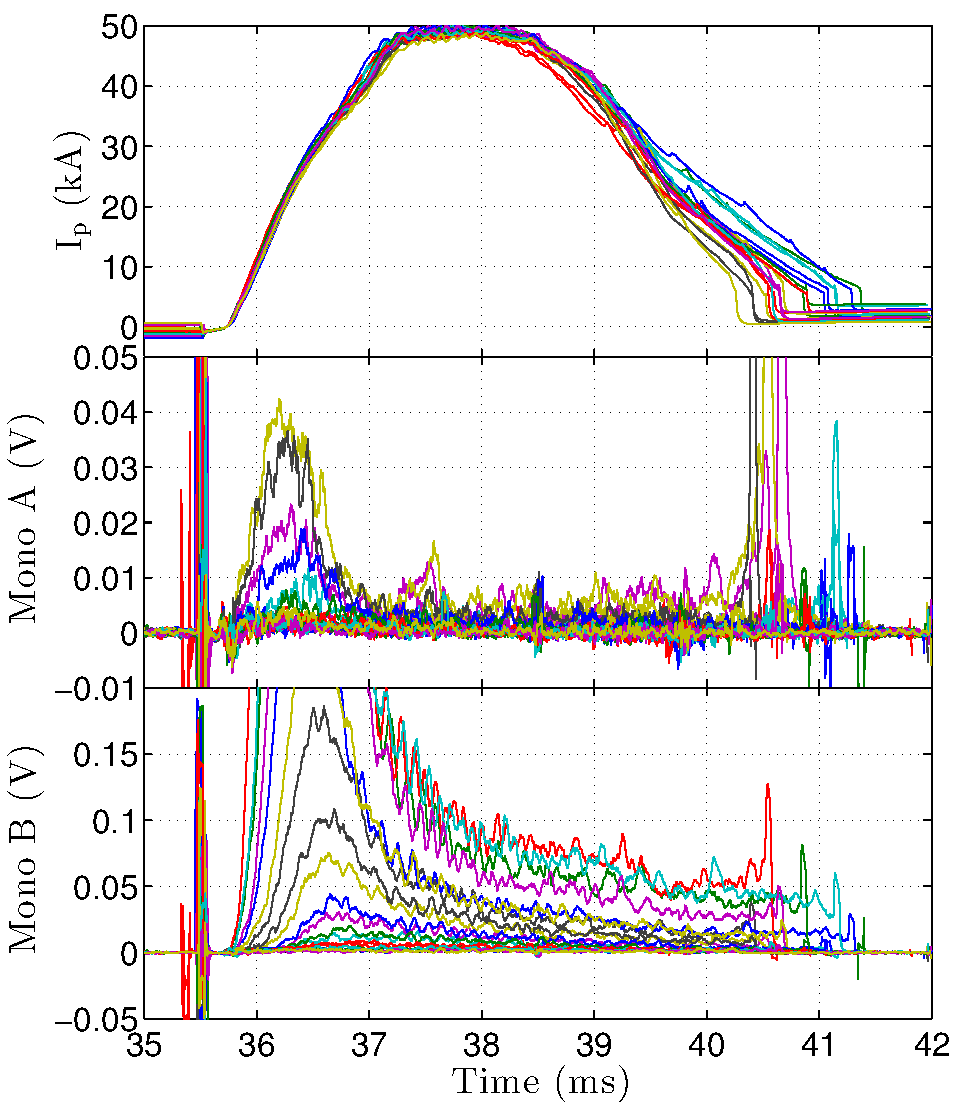
\includegraphics[width=0.7\textwidth]{AH72_BH32.pdf}
  \caption{具有三个能级(基态和两个激发态)原子的日冕图像、碰撞辐射图像和局域热平衡图像示意图。图片来自\onlinecite{Menhart2000:Thesis}。}
  \label{fig:chap02:plasma_model_region}
\end{figure}

\emph{日冕模型}\quad 在低密度等离子体($n<10^{11}\,{\rm cm}^{-3}$)中,等离子体内原子激发态的自发辐射跃迁几率远高于其碰撞损失过程(激发/退激发)的跃迁几率。所以,模型中仅考虑基态的碰撞激发、电离以及激发态的自发辐射跃迁过程。此时,激发态能级粒子的数密度要远低于基态能级的粒子数密度。

\emph{碰撞辐射模型}\quad 当等离子体密度较高时,碰撞过程反应速率增加。此时原子激发态数密度由碰撞和自发辐射过程的相互竞争决定。在碰撞辐射图像中,激发态原子的激发、退激发和电离过程等反应开始变得重要。托卡马克聚变等离子体的密度处在 $10^{11}\,{\rm cm}^{-3}\sim 10^{16}\,{\rm cm}^{-3}$ 区间,其原子反应过程应使用碰撞辐射模型描述。

\emph{局域热平衡模型}\quad 当等离子体密度高于 $10^{18}\,{\rm cm}^{-3}$ 时,碰撞反应过程的速率进一步加大,甚至超过自发辐射跃迁过程,此时激发态原子的自发辐射跃迁过程可以忽略。此时,原子激发态与基态之间处于局域热平衡状态。原子激发态之间和电离态之间的粒子数密度分布分别为麦克斯韦分布和萨哈分布,其分布函数可在 \onlinecite{YuChangxuan:book} 中找到。

\subsection{谱线辐射在等离子体内的传播}

激发态自发辐射跃迁产生的光子在等离子体的传播过程一般需要复杂的辐射输运方程进行描述\cite{Holstein1947:PhysRev.72.1212,Holstein1951:PhysRev.83.1159,Phelps1958:PhysRev.110.1362}。
实际计算中,人们一般采取简化的处理方法,如使用光学厚度和逃逸因子描述等离子体对光子辐射的吸收\cite{Johnson1972:collisionalstrength,boivin2001}。

其中,光学逃逸因子 $\Lambda$(optical escape factor)表示可以逃离等离子体区域的光子与总辐射光子的比例,逃逸因子接近或等于 $1$ 时,等离子体即为光性薄的。平均光学厚度 $\tau_0$(mean optical depth)为等离子体对光谱的指数吸收因子($I=I_0{\rm e}^{-\tau_0}$),当 $\tau_0\le0.01$ 时,对应的等离子体为光性薄的。

%要对逃逸因子和光学厚度进行计算,需要针对每条谱线辐射列出响应的辐射和吸收输运方程。
对于氦等离子体,如果谱线的多普勒展宽为主要展宽机制时\cite{Wiese1966:book},平均光学厚度和光学逃跑因子可以用下列公式计算\cite{Drawin1973:OEF,boivin2001}:
\begin{align}
  \tau_0&=\frac{n_ig_jA_{ji}\lambda_{ji,0}^3r}{8g_i\pi^{3/2}v_{\rm th}} \label{eq:chap02:mod}\\
  \Lambda&=1-\left(\frac{\tau_0}{\sqrt{2}}-\frac{\tau_0^2}{2!\sqrt{3}}+\frac{\tau_0^3}{3!\sqrt{4}}\cdots\frac{(-1)^{n+1}\tau_0^n}{n!\sqrt{n+1}}\right)
\end{align}
其中,$n_i$ 为跃迁低能级的粒子数密度,$g_j$ 和 $g_i$ 分别为跃迁对应高能级和低能级的统计权重,$\lambda_{ji,0}$ 为谱线的中心波长,$v_{\rm th}$ 为氦原子的热速度,$r$ 为等离子体特征尺度(半径)。另外,当谱线的主要展宽机制为非多普勒展宽时,J. He 等人\cite{HeJian2006:ef}计算了氦谱线辐射为洛仑兹(Lorentzian)和沃伊特(Voigt)线形时的逃逸因子。

\section{碰撞辐射模型}

%\subsection{原子反应速率方程}
托卡马克等离子体中的原子反应过程一般由碰撞辐射模型描述,对于等离子体内的某电离态离子的激发态能级粒子 $p$,其数密度 $N_p$ 随时间的变化由下面的速率方程决定:
\begin{equation}
\begin{aligned}
  \frac{{\rm d}N_p}{{\rm d}t}=
  &-\left\{\sum_{q\ne p}C_{pq}N_{\rm e}+\sum_{q<p}A_{pq}+S_{p\nu}N_{\rm e}+r_{p\mu}N_{\rm e}\right\}N_p\\
  &+\left\{\sum_{q\ne p}C_{qp}N_q+\sum_{q>p}A_{qp}N_q\right\}+\left\{S_{\mu p}N_{\mu}+r_{\nu p}N_\nu\right\}N_{\rm e}
\end{aligned}
\end{equation}
其中,$C$、$A$、$S$、$r$ 和 $N$ 分别表示电子碰撞激发或退激发速率系数、自发辐射跃迁几率、电子碰撞电离速率系数、电子碰撞复合速率系数和粒子数密度;下标中 $q$、$\mu$、$\nu$ 和 ${\rm e}$ 分别表示与 $p$ 能级具有相同电离态的 $q$ 激发态能级离子(或原子,下同)、低电离态离子、高电离态离子和电子。可见,对于 $p$ 能级粒子,其主要损失过程包括电子碰撞激发或退激发、电离和复合以及自发辐射跃迁过程;其产生过程也类似地由这些过程决定。

将等离子体内此电离态的基态和亚稳态粒子记为 $\rho$(在碰撞辐射模型中,亚稳态与其他普通激发态粒子的处理没有本质不同,其特性由原子反应过程的速率系数体现),其他激发态粒子记为 $i$,高电离态离子记为 $\nu$,低电离态粒子记为 $\mu$。对每个粒子的数密度 $N$ 列出其速率方程,即可得以下完备的粒子反应速率方程\cite{Summers2006}:
\begin{equation}
\label{eq:chap02:gcr}
\frac{{\rm d}}{{\rm d}t}
\begin{bmatrix}N_\mu\\ N_\rho\\ N_i\\ N_\nu\end{bmatrix}
=
\begin{bmatrix}
	\mathcal{C}_{\mu'} 	& N_{\rm e}\mathcal{R}_{\rho'\mu} & 0 & 0 \\
	N_{\rm e}\mathcal{S}_{\mu'\rho} & \mathcal{C}_{\rho'} & \mathcal{C}_{i'\rho} & N_e\mathcal{R}_{\nu'\rho} \\
	0 & \mathcal{C}_{\rho'i} & \mathcal{C}_{i'} & N_{\rm e}\mathcal{R}_{\nu'i} \\
	0 & N_{\rm e}\mathcal{S}_{\rho'\nu} & N_{\rm e}\mathcal{S}_{i'\nu} & \mathcal{C}_{\nu'}
\end{bmatrix}
\begin{bmatrix}
	N_{\mu'}\\ N_{\rho'}\\ N_{i'}\\ N_{\nu'}
\end{bmatrix}
\end{equation}
其中,方程右侧第一项碰撞辐射矩阵中,$\mathcal{S}$ 与 $\mathcal{R}$ 分别为离子的电离和复合速率系数向量。非对角元素 $\mathcal{C}$ 表示电子碰撞激发/退激发和自发辐射跃迁速率系数向量,以 $\mathcal{C}_{\rho'i}$ 为例:
\begin{equation}
  \mathcal{C}_{\rho'i}=\sum_{\rho'\ne i}C_{\rho'i}N_{\rm e}+\sum_{\rho'>i}A_{\rho'i}
\end{equation}
对角元素表示此粒子的总损失速率,以 $\mathcal{C}_{\rho'}$ 为例:
\begin{equation}
  \mathcal{C}_{\rho'}=-\left\{\left(\mathcal{R}_{\rho'\mu}+\mathcal{S}_{\rho'\nu}\right)N_{\rm e}+\mathcal{C}_{\rho'i}\right\}
\end{equation}
另外,粒子上标 $'$ 表示上一时刻的粒子数密度。

方程 (\ref{eq:chap02:gcr}) 描述了等离子体内各能级粒子(离子)的数密度随时间的变化。其中包含了两个假设:1)模型中只包含只有一个电子得失的电离和复合过程;2)电离和复合过程的产物粒子只处于基态或亚稳态。通过求解此方程可以获得随时间的演化情况,也可以计算系统达到稳态时的结果。对于达到平衡的磁约束聚变等离子体而言,等离子体中粒子碰撞和辐射跃迁过程的时间常数远小于等离子体的粒子约束时间,人们一般采用反应速率方程达到稳态时的计算结果。

%\section{前人在氦原子碰撞辐射模型研究中存在的问题}
\section{氦原子碰撞辐射模型在诊断应用中存在的问题}
\label{sec:chap02:crm-problem}
%\subsection{}

在利用氦原子谱线比诊断托卡马克等离子体 $T_{\rm e}$ 和 $N_{\rm e}$ 的研究中,为了得到更高精度的计算结果,人们不断尝试改进原子反应速率系数的精度,并增加在碰撞辐射模型中包含的能级粒子、反应过程以及可以对原子能级产生影响的因素。但因为使用的截面数据精度不一,导致碰撞辐射模型中包含更多的能级和反应过程时,并不能如预期那样获得更高精度的计算结果(图 \ref{fig:chap02:lineratio-compare-n3})。
%人们不断尝试改进原子反应速率系数的精度,并增加在碰撞辐射模型中包含的能级粒子,以期得到更高精度的激发态粒子数密度计算结果。

\begin{figure}%[H]
  \centering
  \begin{overpic}[width=\textwidth]{lineratio-compare-n3-black.pdf}
  \end{overpic}
  \caption{不同碰撞辐射模型计算的来自 $n=3$ 壳层的谱线比结果对比。(a):$T_{\rm e}=20\,{\rm eV}$ 时,$N_{\rm e}$ 敏感谱线比 $I_{667.8}/I_{728.1}$ 的对比;(b):$N_{\rm e}=1.0\times10^{12}\,{\rm cm}^{-3}$ 时,$T_{\rm e}$ 敏感谱线比 $I_{728.1}/I_{706.7}$ 的对比。模型和数据来源:Schweer1992:来自 \onlinecite{Schweer1992174} ($n\le4$);NIFS($n\le4$):来自 \onlinecite{Sasaki:NIFS:DATA:049};NIFS($n\le20$):来自 \onlinecite{Sasaki:NIFS:DATA:049};Kubo1999:来自 \onlinecite{Hirotaka1999-HeCRM-JT60U},使用 \onlinecite{Fujimoto1979-HeCR} 的模型;Ma2012:来自 \onlinecite{MaShuiliang2012:Tomography},使用 \onlinecite{Goto2003-HeCRM} 的模型;Burgos2012:来自 \onlinecite{burgos2012:PoP};CRM:本文碰撞辐射模型。}
  \label{fig:chap02:lineratio-compare-n3}
\end{figure}


1)原子反应速率系数不确定性

原子反应速率系数(或截面)数据主要有以下三种来源:实验测量
\cite{Shah1988:ionizaiton-data-measure,Long1970:PhysRevA.1.260,Dixon1976}、
理论计算\cite{CCCmethod,Sawey199381}与半经验公式拟合\cite{Fujimoto:IPPJ-AM-8},并且有人对此专门做过总结
\cite{IAEA:Data:vol3,deHeer:INDC,Kato:NIFS:DATA:346}。图 \ref{fig:chap02:xsec-compare} 所示为不同数据来源的电子碰撞激发和速率系数的对比。在碰撞辐射模型方面,人们也在一直将最新的速率系数总结结果应用在计算中,例如,M. Goto\cite{Goto2003-HeCRM} 将以前的碰撞辐射模型\cite{Fujimoto1979-HeCR} 使用的反应速率系数数据进行了更新。然而这些数据来源的精度难以保证\cite{Ralchenko2008603},导致不同来源原子反应数据的碰撞辐射其计算结果也不尽相同\cite{Delabie2010:consistency}。%如第 \ref{sec:chap01:research-history} 节所述,

碰撞辐射模型中包含着数目巨大的激发态能级和复杂的相关反应过程,且各粒子之间通过原子反应相互关联。目前并没有有效的手段可以对速率系数不确定性至激发态数密度计算误差之间的传递进行计算。Y. Andrew 等人\cite{Andrew2000PPCFSensitivity}提出了一种计算方法,在假设碰撞辐射模型中某一过程的速率系数具有不确定性时,对此速率系数进行干扰,并重新求解碰撞辐射模型,以获得该速率系数的不确定性对粒子数密度计算的影响。通过对所有的速率系数进行干扰并重新求解碰撞辐射模型,即可得到模型中各反应过程速率系数的影响。这种方法并不直观,速率系数不确定性至激发态数密度计算误差传递之间的物理意义不明确,且每次都要对碰撞辐射模型进行重新求解,也不能对速率系数精度提出具体的要求。

\begin{figure}%[H]
  \centering
  \begin{subfigure}{0.45\textwidth}
  \begin{overpic}[width=\textwidth]{meta-exc-xsec-compare.pdf}
    \put(30,0){\mbox{\colorbox{white}{\small\hspace{2em}$T_{\rm e} (${\rm eV}$)$\hspace{2em}}}}
    \put(-2,30){\rotatebox{90}{\mbox{\colorbox{white}{\small\hspace{2em}激发截面 (${\rm m}^2$)\hspace{2em}}}}}
  \end{overpic}
  \caption{电子碰撞激发 $2^3{\rm S}\to 3^3{\rm D}$ 的截面}
  \label{fig:chap02:xsec-compare-meta}
  \end{subfigure}
  \hspace{0.03\textwidth}
  \begin{subfigure}{0.45\textwidth}
  \begin{overpic}[width=\textwidth]{l-change-exc-rate-compare.pdf}
    \put(30,0){\mbox{\colorbox{white}{\small\hspace{2em}$T_{\rm e} (${\rm eV}$)$\hspace{2em}}}}
    \put(-2,25){\rotatebox{90}{\mbox{\colorbox{white}{\small\hspace{2em}激发速率系数 (${\rm m}^3/{\rm s}$)\hspace{2em}}}}}
  \end{overpic}
  \caption{电子碰撞激发 $3^3{\rm S}\to 3^3{\rm P}$ 的速率系数}
  \label{fig:chap02:xsec-compare-l-change}
  \end{subfigure}
  \caption{不同数据来源的电子碰撞激发和速率系数数据对比。图片来自
  \onlinecite{Goto1997-HeCRM-WT3},数据来源详见 \onlinecite{Goto1997-HeCRM-WT3} 的参考文献。}
  \label{fig:chap02:xsec-compare}
\end{figure}

2)模型中包含的激发态能级和反应过程

最早人们使用最高包含至 $n=4$ 壳层的碰撞辐射模型\cite{Brosda1993:Thesis,Schweer1992174},后来在模型中增加了 $5\le n\le9$ 的激发态和 ${\rm He}^+$\cite{Schmitz2008},随着模型的发展,包含了越来越多的能级\cite{Ahn2007-He-BES},甚至最高包含到了 $n=500$ 壳层的能级\cite{burgos2012:PoP}。然而,通过将这些模型谱线比的计算结果进行对比(图 \ref{fig:chap02:lineratio-compare-n3})发现,这些模型并没有因为包含了跟多的能级和反应过程而获得高精度的结果。

首先,对于很高激发态的能级,现阶段无法对其电子碰撞激发或电离的截面进行精确的理论计算,实验更是无法进行测量。模型中,只能通过经验上的定标关系来计算,然而这种定标关系的精度是很难保证的。其次,对于高激发态能级,其粒子数密度会急剧减少\cite{Fujimoto1979-HeCR,Griem1964-book},然而在模型中使用低精度的反应截面数据将其包含在计算中,这不但不会带来更高精度的计算结果,反而可能会带来更大的计算误差。目前,在使用相同的速率系数的前提下,在模型中包含不同的能级和反应过程对计算结果影响的研究还鲜有报道。其中,文献  \onlinecite{Sasaki:NIFS:DATA:049} 中给出了模型包含 $n\le4$ 和 $n\le20$ 时不同的计算结果,但没有详细分析模型中包含不同能级粒子时,计算结果将会呈现什么样的趋势。


\section{小结}

本章首先介绍了可同时诊断等离子体电子温度与密度的原子谱线辐射强度比法,然后从光子产生到被光谱测量设备探测接收所经历的物理过程出发,给出影响谱线强度的因素,包括:自发辐射跃迁几率、光子在等离子体内传播过程中的再吸收和激发态粒子数密度。其中,自发辐射跃迁几率系数可以获得高精度的数据,对于光性薄的等离子体,激发态粒子数密度与其电子密度和电子温度参数相关,通过建立描述等离子体内各粒子的原子反应速率方程,即可以求解出在不同的等离子体参数情况下的激发态粒子数密度。通过实验测量来自不同激发态的谱线,根据其谱线强度比,既可以反推出等离子体的电子温度和密度参数。

在实际研究中,人们根据等离子体密度的不同对等离子体内的反应过程进行不同的简化。对高温聚变等离子体,需要使用碰撞辐射模型以计入原子碰撞激发/退激发、电离/复合以及自发辐射跃迁等过程,以求解激发态粒子数密度。然而,原子反应过程速率系数(截面)数据的精度受到很大限制,以致人们在模型中包含越来越多的能级粒子和反应过程,却不能如预期的那样得到更高精度的结果。同时,由于碰撞辐射模型中包含了数目巨大的能级粒子和复杂的反应过程,目前并无有效手段对速率系数不确定性至能级粒子数密度计算误差的传递进行直接的有效计算。一般使用对速率系数进行干扰并再次求解模型的速率方程的方法,这种分析手段并不直观,也不易操作,对不确定性的传递也不能给出明确的物理意义。


\graphicspath{{figures/chap03/}}

\chapter{SUNIST 参数范围下氦原子碰撞辐射模型的研究}%的建立与研究}%与谱线比法
\label{chap:crmodel}

针对具有 SUNIST 参数范围的氦放电等离子体,建立了氦原子的碰撞辐射模型。首先通过对各原子过程反应速率进行分析,忽略了杂质粒子的影响,为氦原子各能级粒子选定了相应的反应过程,列出粒子数反应速率方程,并计算出反应过程相应的反应速率系数。基于对各能级的主要产生过程的分析,推导得出反应速率系数不确定性的传递函数,通过对比包含不同能级数目时碰撞辐射模型的计算,根据反应速率系数不确定性的传递结果,给出模型只需最高包含至 $\max n=7$ 即可以给出满足 SUNIST 参数条件下使用来自 $n=4$ 激发态能级谱线比诊断所要求的能级粒子数密度计算精度。最后,给出同时获得 $T_{\rm e}$ 和 $N_{\rm e}$ 参数的谱线比法。

%\section{引言}

\section{氦原子碰撞辐射模型的建立}

\subsection{氦原子的能级分布与能级结构处理}
\label{sec:chap03:level-selection}

\begin{figure}%[H]
  \centering
%  \begin{overpic}[width=0.7\textwidth]{he-exc-xsec-compare.pdf}
%    \put(45,1){\mbox{\colorbox{white}{能量 (${\rm eV}$)}}}
%    \put(-2,25){\rotatebox{90}{\mbox{\colorbox{white}{碰撞截面 (${\rm cm}^2$)}}}}
%  \end{overpic}
  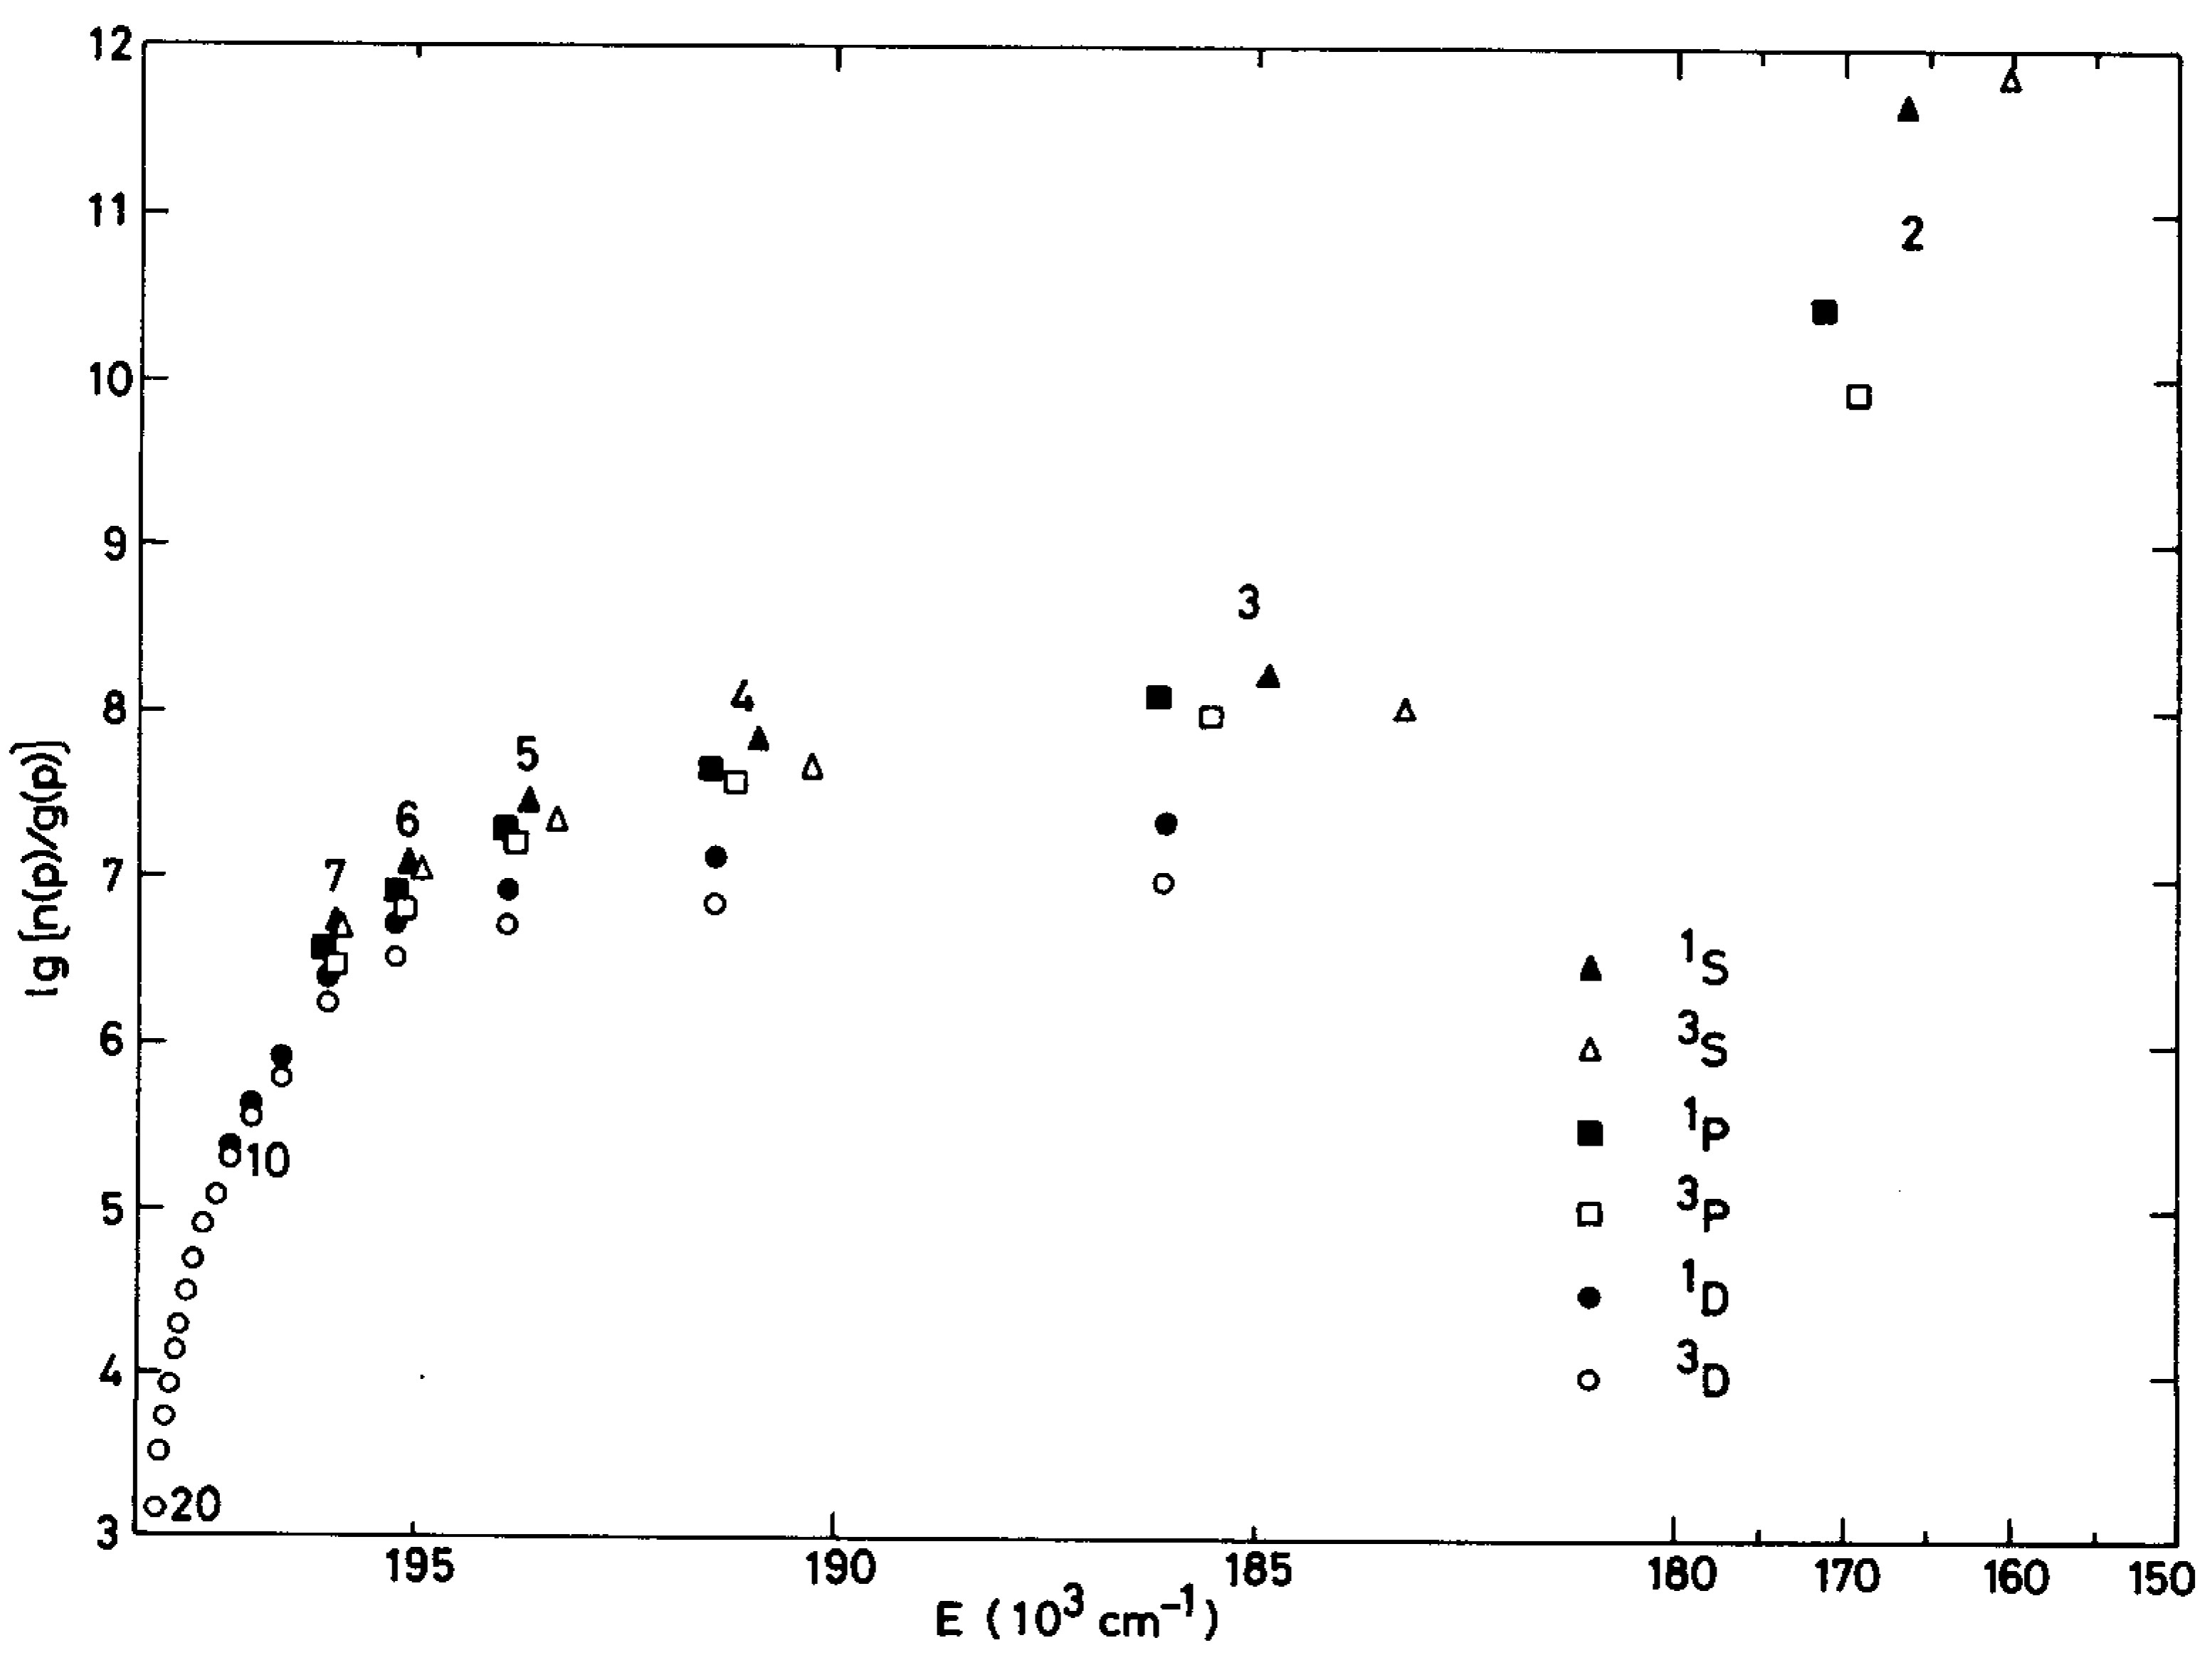
\includegraphics[width=0.7\textwidth]{fujimoto-level-distribution.jpg}
  \caption{T. Fujimoto 对氦原子能级数密度的计算结果。对应放电管(直径 $R=0.8\,{\rm cm}$)实验参数为气压 $53.3\,{\rm Pa}$、放电电流 $100\,{\rm mA}$。放电管中心的基态氦原子数密度为 $1.2\times10^{16}\,{\rm cm}^{-3}$、 电子密度为 $6.3\times10^{10}\,{\rm cm}^{-3}$、 电子温度为 $4.9\,{\rm eV}$。 图片来自\onlinecite{Fujimoto1979-HeCR}。}
  \label{fig:chap03:fujimoto-level-distribution}
\end{figure}

图 \ref{fig:chap03:fujimoto-level-distribution} 显示的是 T. Fujimoto 的碰撞辐射模型\cite{Fujimoto1979-HeCR} 对一个放电管中氦原子能级数密度分布的计算结果。根据 H. R. Griem 提出的原则\cite{Griem1964-book},给出了一个临界能级主量子数:
\begin{equation}\label{eq:chap03:criticalLevel}
    n_c=\left(\frac{8\cdot10^{17}}{N_{\rm e}}\right)^{2/17}
        \left(\frac{kT_{\rm e}}{\chi_H}\right)^{1/17} ,
\end{equation}
其中,$\chi_H$ 为氢的基态电离能,$k$ 为玻尔兹曼常数。主量子数处于 $n_c$ 以下的能级粒子数密度与能级的能量之间无明显的函数关系(除基态与亚稳态外 $N_p/g_p\propto n^{-0.5}$,其中,$N_p$ 与$g_p$ 分别为 $p$ 激发态的数密度和统计权重因子,$n$ 为 $p$ 激发态能级的主量子数),其能级粒子数由激发态粒子之间电子碰撞跃迁与自发辐射过程共同决定,称为日冕区~(corona phase)能级。主量子数处于 $n_c$ 以上能级的粒子数密度随能级的升高而快速下降($N_p/g_p\propto n^{-6}$),其粒子之间的电子碰撞跃迁过程大于自发辐射过程,称为准饱和区(quasi-saturation phase)能级。对于SUNIST 等离子体,在高密度低温等离子体条件下 $n_c=4$;在低密度高温等离子体条件下 $n_c=6$。基于此结论,本文的 CR 模型包含主量子数 $n\le 7$ 的所有激发态能级(第 \ref{sec:chap03:maxn-in-crm} 节将给出更多的讨论)以及氦的两个离子 ${\rm He}^+$ 与${\rm He}^{2+}$,将轨道角动量 $l\ge 3$ 的能级合并成为一个能级,记为 ${\rm F}^+$ 能级。
图 \ref{fig:chap03:he-level-diagram} 所示为本文模型的氦原子能级图。

\begin{figure}
  \centering
  \begin{overpic}[width=0.7\textwidth]{He-diagrames-plus-wlxb-en.pdf}
    \put(20,1){\mbox{\colorbox{white}{\quad 自旋单重态\quad}}}
    \put(60,1){\mbox{\colorbox{white}{\quad 自旋三重态\quad}}}
    \put(-1,32){\rotatebox{90}{\mbox{\colorbox{white}{\quad 能量 (${\rm eV}$)}}}}
    \put(53.7,86.8){$^+$}
    \put(88.9,86.8){$^+$}
  \end{overpic}
  %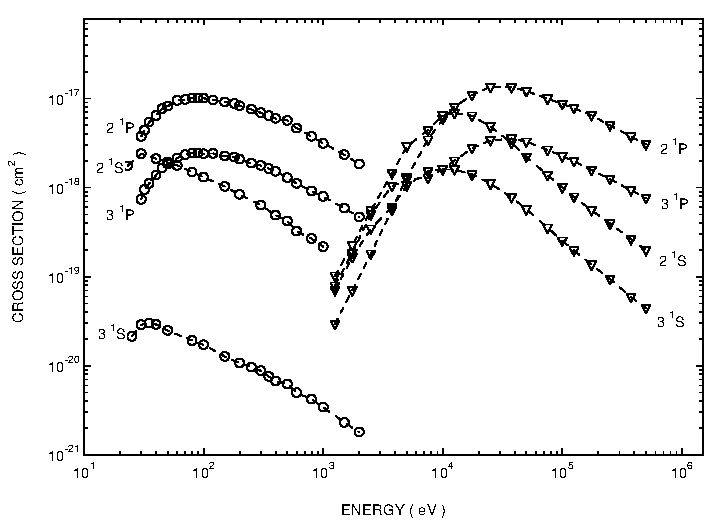
\includegraphics[width=0.7\textwidth]{he-exc-xsec-compare.pdf}
  \caption{本文碰撞辐射模型使用的氦原子能级图。图片来自\onlinecite{xie:wlxb},能级数据来自\onlinecite{NISTdatabase}。}
  \label{fig:chap03:he-level-diagram}
\end{figure}


%\subsection{忽略氢及其他杂质粒子的影响}
%\subsection{SUNIST 等离子体原子反应过程选择及等离子体的光性厚度}

%真空室内的水与氢气是较难去除的。

%\subsection{SUNIST 等离子体原子激发和电离过程的选择}
\subsection{氦原子激发和电离过程的选择}

影响氦原子数密度的首先是碰撞电离过程,可以将氦原子内的电子剥离的反应过程如下\cite{Anderson1999:Thesis}:
\begin{enumerate}
  \item 电子碰撞电离与双电离\\
        ${\rm e}+{\rm He}\to {\rm e}+{\rm He}^+ + {\rm e}$\\
        ${\rm e}+{\rm He}\to {\rm e}+{\rm He}^{2+} + {\rm e} + {\rm e}$
  \item 离子碰撞电离与双电离\\
        ${\rm X}^{+z_0} + {\rm He} \to {\rm X}^{+z_0} + {\rm He}^+ + {\rm e}$\\
        ${\rm X}^{+z_0} + {\rm He} \to {\rm X}^{+z_0} + {\rm He}^{2+} + {\rm e} + {\rm e}$
  \item 单电子与双电子电荷交换\\
        ${\rm X}^{+z_0} + {\rm He} \to {\rm X}^{+z_0-1} + {\rm He}^+ $\\
        ${\rm X}^{+z_0} + {\rm He} \to {\rm X}^{+z_0-2} + {\rm He}^{2+}$
  \item 电子交换双电离(transfer double ionization)\\
        ${\rm X}^{+z_0} + {\rm He} \to {\rm X}^{+z_0-1} + {\rm He}^{2+} + {\rm e}$
\end{enumerate}
其中,${\rm X}$ 表示某杂质原子或离子。

影响氦原子激发态数密度的是碰撞激发、退激发以及自发辐射跃迁过程,其主要反应如下\cite{Anderson1999:Thesis}:
\begin{enumerate}
  \item[5.] 电子与离子碰撞激发与退激发\\
        ${\rm e}+{\rm He}(n\,^{\rm 2S+1}{L}) \leftrightarrow {\rm e}+{\rm He}(n\,^{\rm 2S+1}{L})$\\
        ${\rm X}^{+z_0} + {\rm He}(n\,^{1}L) \leftrightarrow {\rm X}^{+z_0} + {\rm He}(n\,^{1}L)$
  \item[6.] 自发辐射跃迁\\
        ${\rm He}(n\,^{\rm 2S+1}L) \to  {\rm He}(n\,^{\rm 2S+1}L) + h\nu$
\end{enumerate}
其中,电子碰撞可以产生自旋变化跃迁,而离子碰撞只能在相同的自旋能级粒子之间发生跃迁。

以上每个反应过程,对于特定的 $p$ 能级粒子,其粒子数密度 $N_p$ 变化速率为:
\begin{equation}
  \frac{{\rm d}\,N_p}{{\rm d}\,t}=-n_{\rm e,X}\cdot N_p\cdot <v_{\rm e,X}\cdot\sigma_{pq}>
  \label{eq:chap03:p-rate-eq}
\end{equation}
其中,$n_{\rm e,X}$ 为电子或重粒子的数密度,$v_{\rm e,X}$ 为电子或重粒子的碰撞速度,$\sigma_{pq}$ 为 $p\to q$ 反应过程的碰撞截面。可以看出,在碰撞辐射模型中,影响激发态能级粒子数密度的过程主要受 $n_{\rm e,X}$、$N_p$、$v_{\rm e,X}$ 和 $\sigma_{pq}$ 四个因素乘积的影响。下面我们将对这些因素做详细分析,分析过程中将氦原子的基态(${\rm gs}$)、亚稳态(${\rm meta}$)和普通激发态 $p$ 进行分别讨论。

\begin{figure}
  \centering
  \begin{overpic}[width=\textwidth]{rel-levelabun-thesis.pdf}
  \end{overpic}
  %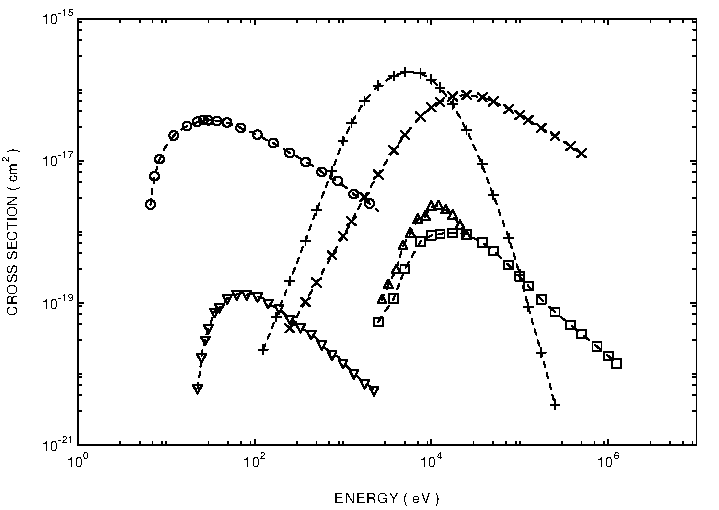
\includegraphics[width=0.7\textwidth]{he-ionization-xsec-comapre.pdf}
  \caption{氦等离子体中 $n\le3$ 各能级和氦离子(${\rm He}^{+}$ 和 ${\rm He}^{2+}$)相对含量随电子温度和电子密度的变化趋势。(a):$T_{\rm e}=20\,{\rm eV}$ 时随电子密度的变化;(b):$N_{\rm e}=1.0\times10^{12}\,{\rm cm}^{-3}$ 时随电子温度的变化。}
  \label{fig:chap03:rel-levelabun-compare}
\end{figure}

1)粒子数密度的量级

图 \ref{fig:chap03:rel-levelabun-compare} 所示为碰撞辐射模型对氦等离子体中 $n\le3$ 各能级粒子和氦离子(${\rm He}^{+}$ 和 ${\rm He}^{2+}$)相对含量随 $T_{\rm e}$ 和 $N_{\rm e}$ 的变化趋势计算结果。可以看出在 SUNIST 等离子体参数范围内,当 $T_{\rm e}=20\,{\rm eV}$ 时,由于电子碰撞激发,普通激发态粒子数密度随 $N_{\rm e}$ 增大而增加,基态和亚稳态由于电子碰撞激发过程的影响,其粒子数密度相对略有下降。在特定的 $N_{\rm e}$ 条件下($1.0\times10^{12}\,{\rm cm}^{-3}$),随着 $T_{\rm e}$ 的上升,各氦原子能级数密度快速下降。我们将以图 \ref{fig:chap03:rel-levelabun-compare}(a) 所示做氦原子和氦离子的数密度量级估计,SUNIST 氦放电等离子体中,可以认为 $N_{\rm e}$ 与 ${\rm He}^{2+}$ 具有相同量级的数密度。

对于 SUNIST 真空室,连续放电后,质谱测量结果显示等效氢原子数占本底原子数约为 $40\%$,为氦等离子体放电时的主要杂质。本底气压在小于 $1\times10^{-4}\,{\rm Pa}$ 范围内,放电时的气压约为 $4.5\times10^{-3}\,{\rm Pa}$,可见,正常放电时 H 的数密度比 $N_{{\rm He}^{2+}}$ 要小两个数量级,同时,由于其他如 C、N、O 等杂质含量不会高于氢\cite{Isler1984:NF:Impurities},我们这里将这些杂质粒子的数密度量级设为与 H 相同。

表 \ref{table:chap03:N-gusuan} 所示为 SUNIST 氦放电等离子体各粒子数密度量级的估算结果,在量级估算时,以基态能级粒子数密度 $N_{\rm gs}$ 为基准。

\begin{table}%[H]
\caption{氦等离子体各粒子数密度的量级}
\label{table:chap03:N-gusuan}
\begin{center}
\begin{tabular}{lcc}\toprule[1.5pt]
粒子数密度 & & 量级 \\
\midrule[1pt]
\hspace{1.5em}$N_{\rm gs}$ & & \hspace{0.5em}$0$ \\
\hspace{1.5em}$N_{\rm meta}$ & & \hspace{0.5em}$-1^{*}$ \\
\hspace{1.5em}$N_p$ & & $-4$ \\
\hspace{1.5em}$N_{{\rm He}^{2+}}$ & & $+6$ \\
\hspace{1.5em}$N_{\rm X}$ & & $+4$ \\
\hspace{1.5em}$N_{\rm e}$ & & $+6$\\
\bottomrule[1.5pt]
\end{tabular}\\[0.5em]
{\small$*$:$-1$ 表示该粒子数密度的量级为基准数密度的 $10^{-1}$。}
\end{center}
\end{table}

2)碰撞速度的量级

对于 SUNIST 等离子体,电子与离子的热平衡弛豫时间常数为 $\tau_{\rm i-e}\sim2\,{\rm ms}$ (第 \ref{sec:chap03:quasi-stationary} 节),与 SUNIST 放电平顶段持续时间相同,可以认为离子温度是远小于电子温度的,则电子与重粒子的碰撞速度应有三个量级的差别。重粒子主要为 H、He、C、N 和 O 等轻元素,不妨认为他们具有相同量级的碰撞速度。以电子碰撞速度 $v_{\rm e}$ 为基准,表 \ref{table:chap03:v-gusuan} 所示为碰撞速度的量级结果。

\begin{table}%[H]
\caption{各粒子碰撞速度的量级}
\label{table:chap03:v-gusuan}
\begin{center}
\begin{tabular}{lcc}\toprule[1.5pt]
碰撞速度 & & 量级 \\
\midrule[1pt]
\hspace{1.5em}$v_{\rm e}$ & & \hspace{0.5em}$0$ \\
\hspace{1.5em}$v_{\rm He}$ & & $-3$ \\
\hspace{1.5em}$v_{\rm X}$ & & $-3$ \\
\bottomrule[1.5pt]
\end{tabular}
\end{center}
\end{table}

3)碰撞截面的量级

\begin{figure}
  \centering
  \begin{overpic}[width=0.7\textwidth]{he-ionization-xsec-comapre.pdf}
    \put(45,1){\mbox{\colorbox{white}{能量 (${\rm eV}$)}}}
    \put(-3,25){\rotatebox{90}{\mbox{\colorbox{white}{碰撞截面 (${\rm cm}^2$)}}}}
  \end{overpic}
  %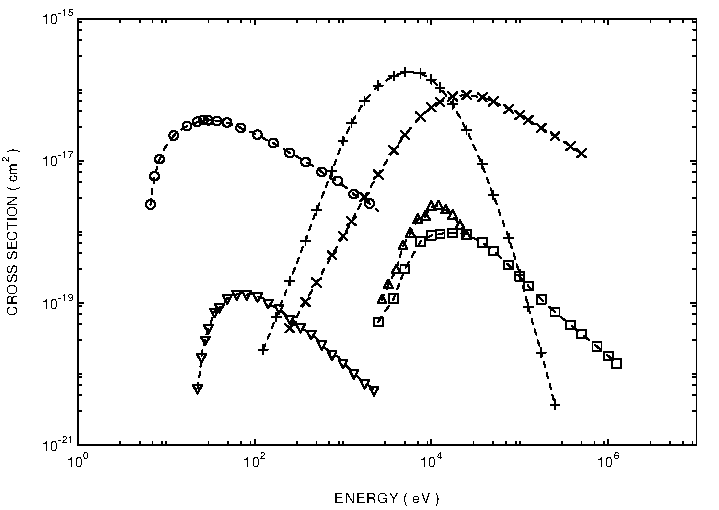
\includegraphics[width=0.7\textwidth]{he-ionization-xsec-comapre.pdf}
  \caption{氦原子基态($1^1{\rm S}$)的电子与氢离子(质子)碰撞电离反应截面数据。$\circ$:电子碰撞电离;$\triangledown$:电子碰撞双电离;$+$:单电子电荷交换;$\times$:质子碰撞电离;$\triangle$:电子交换双电离;$\Box$:质子碰撞双电子电离。图片来自
  \onlinecite{Anderson1999:Thesis}。}
  \label{fig:chap03:he-ion-xsec-compare}
\end{figure}

图 \ref{fig:chap03:he-ion-xsec-compare} 所示为氦原子的电子与质子碰撞电离过程截面数据。可以看出,在几十至几百电子伏的温度范围,电子碰撞电离过程的截面远大于其他反应过程。电子碰撞双电离过程的截面虽然低两个数量级,但也比质子碰撞电离过程截面要大。只有当温度达到 $\sim750\,{\rm eV}$ 及以上时,单电子电荷交换过程才变得重要,并且质子碰撞电离过程与其相当,直到温度达 $20\,{\rm keV}$ 以上,质子碰撞电离过程的截面超过电荷交换过程。

\begin{figure}
  \centering
  \begin{overpic}[width=0.7\textwidth]{he-exc-xsec-compare.pdf}
    \put(45,1){\mbox{\colorbox{white}{能量 (${\rm eV}$)}}}
    \put(-2,25){\rotatebox{90}{\mbox{\colorbox{white}{碰撞截面 (${\rm cm}^2$)}}}}
  \end{overpic}
  %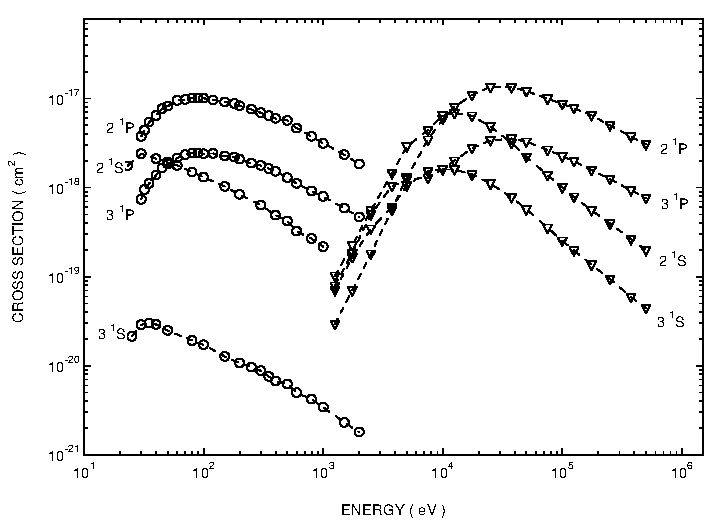
\includegraphics[width=0.7\textwidth]{he-exc-xsec-compare.pdf}
  \caption{氦原子基态($1^1{\rm S}$)的电子与氢离子(质子)碰撞激发截面。$\circ$:电子碰撞激发;$\triangledown$:质子碰撞激发。图片来自\onlinecite{Anderson1999:Thesis}。}
  \label{fig:chap03:he-exc-xsec-compare}
\end{figure}

图 \ref{fig:chap03:he-exc-xsec-compare} 显示的是基态氦原子的电子与质子碰撞激发反应截面。可以看出,只有当温度高于 $1\,{\rm keV}$ 时,质子碰撞激发过程才显得重要。

由此,以电子碰撞激发截面为基准,各激发和电离过程的截面量级在表 \ref{table:chap03:sigma-gusuan} 中列出。

\begin{table}%[H]
\caption{氦原子电子碰撞(${\rm e-}$)和重粒子碰撞(${\rm X-}$)激发、电离过程截面的量级}
\label{table:chap03:sigma-gusuan}
\begin{center}
\begin{tabular}{lcc}\toprule[1.5pt]
碰撞截面$^*$ & & 量级 \\
\midrule[1pt]
\hspace{0.5em}$\sigma_{\rm e-exc}$ & & \hspace{0.5em}$0$ \\
\hspace{0.5em}$\sigma_{\rm X-exc}$ & & $-3$ \\%[1em]
\hspace{0.5em}$\sigma_{\rm e-ion}$ & & $+1$ \\
\hspace{0.5em}$\sigma_{\rm e-dbion}$ & & $-2$ \\
\hspace{0.5em}$\sigma_{\rm X-ion}$ & & $-3$ \\
\hspace{0.5em}$\sigma_{\rm X-dbion}$ & & $-3$ \\
\bottomrule[1.5pt]
\end{tabular}\\[0.5em]
{\small $*$:其中,${\rm exc}$ 表示激发过程,${\rm ion}$ 表示电离过程,${\rm dbion}$ 表示双电子离过程}
\end{center}
\end{table}

4)电子碰撞与重粒子碰撞激发过程的选择

根据表 \ref{table:chap03:N-gusuan} -- 表 \ref{table:chap03:sigma-gusuan},将电子碰撞和重粒子碰撞的氦原子激发过程及其数密度反应速率量级估算结果在表 \ref{table:chap03:exc-process-gusuan} 中列出。可见,氦原子基态的电子碰撞激发过程占主要部分,而普通激发态能级粒子的电子碰撞激发要低四个量级,重粒子碰撞的激发反应速率则更低。所以在碰撞辐射模型中将重粒子碰撞激发过程忽略是合理的。

\begin{table}%[H]
\caption{氦原子电子碰撞(${\rm e-}$)和重粒子碰撞(${\rm X-}$)激发过程的量级估算}
\label{table:chap03:exc-process-gusuan}
\begin{center}
%{\small 其中,${\rm exc}$ 表示激发过程,${\rm ion}$ 表示电离过程,${\rm dbion}$ 表示双电子离过程}\\
\begin{tabular}{lrrrrc}\toprule[1.5pt]
反应过程 & $n_{\rm e,X}$ & $N_{p}$ & $v_{e,X}$ & $\sigma_{pq}$ & 反应过程量级\\
\midrule[1pt]
${\rm e-}$基态       & $+6$ & $0$  & $0$  & $0$  & $+6$ \\
${\rm e-}$亚稳态     & $+6$ & $-1$ & $0$  & $0$  & $+5$ \\
${\rm e-}$普通激发态 & $+6$ & $-4$ & $0$  & $0$  & $+2$ \\
${\rm X-}$基态       & $+4$ & $0$  & $-3$ & $-3$ & $-2$ \\
${\rm X-}$亚稳态     & $+4$ & $-1$ & $-3$ & $-3$ & $-3$ \\
${\rm X-}$普通激发态 & $+4$ & $-4$ & $-3$ & $-3$ & $-6$ \\
\bottomrule[1.5pt]
\end{tabular}
\end{center}
\end{table}

5)电子碰撞与重粒子碰撞电离过程的选择

将电子碰撞和重粒子碰撞的氦原子电离过程及其数密度速率量级估算结果在表 \ref{table:chap03:ion-process-gusuan} 中列出。可见,对于氦的电离过程,在碰撞辐射模型中,将重粒子碰撞电离、双电离以及除基态外的电子碰撞双电离过程忽略是合理的。

\begin{table}%[H]
\caption{氦原子电子碰撞(${\rm e-}$)和重粒子碰撞(${\rm X-}$)电离过程的量级估算}
\label{table:chap03:ion-process-gusuan}
\begin{center}
%{\small 其中,${\rm exc}$ 表示激发过程,${\rm ion}$ 表示电离过程,${\rm dbion}$ 表示双电子离过程}\\
\begin{tabular}{lrrrrc}\toprule[1.5pt]
反应过程 & $n_{\rm e,X}$ & $N_{p}$ & $v_{e,X}$ & $\sigma_{pq}$ & 反应过程量级\\
\midrule[1pt]
${\rm e-}$基态       & $+6$ & $0$  & $0$  & $+1$ & $+7$ \\
${\rm e-}$亚稳态     & $+6$ & $-1$ & $0$  & $+1$ & $+6$ \\
${\rm e-}$普通激发态 & $+6$ & $-4$ & $0$  & $+1$ & $+3$ \\
${\rm X-}$基态       & $+4$ & $0$  & $-3$ & $-3$ & $-2$ \\
${\rm X-}$亚稳态     & $+4$ & $-1$ & $-3$ & $-3$ & $-3$ \\
${\rm X-}$普通激发态 & $+4$ & $-4$ & $-3$ & $-3$ & $-6$ \\
${\rm e-}$基态(双电离)       & $+6$ & $0$  & $0$  & $-2$  & $+4$ \\
${\rm e-}$亚稳态(双电离)     & $+6$ & $-1$ & $0$  & $-2$  & $+3$ \\
${\rm e-}$普通激发态(双电离) & $+6$ & $-4$ & $0$  & $-2$  & \hspace{0.8em}$0$ \\
${\rm X-}$基态(双电离)       & $+4$ & $0$  & $-3$ & $-3$ & $-2$ \\
${\rm X-}$亚稳态(双电离)     & $+4$ & $-1$ & $-3$ & $-3$ & $-3$ \\
${\rm X-}$普通激发态(双电离) & $+4$ & $-4$ & $-3$ & $-3$ & $-6$ \\
\bottomrule[1.5pt]
\end{tabular}
\end{center}
\end{table}

\subsection{氦放电等离子体光性厚度的计算}

根据式 (\ref{eq:chap02:mod}),计算了在不同的温度和密度组合下平均光性厚度 $\tau_0$ 的数值,如表 \ref{table:chap03:helines-mod} 所示。因为 SUNIST 等离子体中较低的 $n_i$ 与较高的 $v_{\rm th}$,SUNIST 等离子体对测量谱线的吸收作用可以忽略,计算结果还显示即使对跃迁低能级为基态或亚稳态的共振线,仍可以忽略等离子体的吸收影响。

\begin{table}%[H]
\caption{本文测量氦原子谱线的平均光性厚度}
\label{table:chap03:helines-mod}
\begin{center}
\begin{tabular}{ccccccc}
\toprule[1.5pt]
\multirow{3}*{跃迁} & \multirow{3}*{$\lambda_{ji,0}$ (${\rm nm}$)} &
\multicolumn{2}{c}{$\tau_0$ ($10^{-7}$)} & & \multicolumn{2}{c}{$\tau_0$ ($10^{-12}$)} \\
\cmidrule[1pt]{3-4} \cmidrule[1pt]{6-7}
 & & \multicolumn{2}{c}{$T_{\rm e}=30\,{\rm eV}$} & & \multicolumn{2}{c}{$T_{\rm e}=300\,{\rm eV}$}\\
 & & $N_{\rm e}=10^{12}\,{\rm cm}^{-3}$ & $10^{13}\,{\rm cm}^{-3}$ && $N_{\rm e}=10^{12}\,{\rm cm}^{-3}$ & $10^{13}\,{\rm cm}^{-3}$ \\
\midrule[1pt]
$2^1{\rm S}\leftarrow3^1{\rm P}$ & 501.6 & 0.005 & 0.005 && 0.032 & 0.032\\
$2^1{\rm S}\leftarrow4^1{\rm P}$ & 396.5 & 0.001 & 0.001 && 0.008 & 0.008\\
$2^1{\rm P}\leftarrow4^1{\rm S}$ & 504.8 & 0.000 & 0.000 && 0.000 & 0.000\\
$2^1{\rm P}\leftarrow4^1{\rm D}$ & 492.2 & 0.000 & 0.000 && 0.000 & 0.002\\
$2^3{\rm S}\leftarrow3^3{\rm P}$ & 388.9 & 0.442 & 0.116 && 0.242 & 0.083\\
$2^3{\rm P}\leftarrow3^3{\rm D}$ & 587.6 & 0.781 & 1.251 && 0.285 & 0.688\\
$2^3{\rm P}\leftarrow4^3{\rm S}$ & 471.3 & 0.004 & 0.006 && 0.001 & 0.003\\
$2^3{\rm P}\leftarrow4^3{\rm D}$ & 447.1 & 0.120 & 0.192 && 0.044 & 0.105\\
$2^3{\rm P}\leftarrow5^3{\rm S}$ & 412.1 & 0.001 & 0.002 && 0.000 & 0.001\\
\bottomrule[1.5pt]
\end{tabular}
\end{center}
\end{table}

\subsection{氦原子能级数密度反应速率方程的建立}

碰撞辐射模型的核心是对模型中包含的粒子列出其数密度反应速率方程,联立这些方程以求得各粒子的数密度。在氦等离子体中,不同的激发态能级具有不尽相同的主要反应过程,例如 ${\rm He}^{2+}$ 粒子不存在双电子复合过程(dielectric recombination)、电子碰撞双电子电离过程只需计入基态粒子等。本文的碰撞辐射模型针对不同的能级也做了相应的处理。

基态氦原子 $1^1{\rm S}$ 的主要损失过程包括电子碰撞激发与电离;主要产生过程包括激发态电子碰撞退激发和自发辐射跃迁以及 ${\rm He}^+$ 离子的辐射复合(radiation recombination)与偶电子复合(dielectric recombination)过程。其粒子数密度 $N_1$ 的速率方程:
\begin{equation}
    \label{eq:crm:gs}
    \begin{aligned}
        \frac{{\rm d}\,N_1}{{\rm d}\,t}=
        &-\left\{\sum_{q>1}C_{1q}+S_{{\rm He}^+}(1)+S_{{\rm He}^{2+}}(1)\right\}N_{\rm e}N_1\\
        &+\sum_{q>1}\left\{C_{q1}N_{\rm e}+A_{q1}\right\}N_q\\
        &+\left\{\beta_{{\rm He}^+}(1)+\beta_{{\rm He}^+,\rm d}(1)\right\}N_{\rm e}N_{{\rm He}^+}
    \end{aligned}
\end{equation}

对于亚稳态 $2^1{\rm S}$ 和 $2^3{\rm S}$,忽略其与普通激发态的电子碰撞双电子电离与偶电子复合过程,则对于氦原子的激发态和亚稳态 $p$,主要损失过程为电子碰撞激发与退激发、自发辐射跃迁与电子碰撞电离过程;主要产生过程为:电子碰撞激发与退激发,自发辐射跃迁与 ${\rm He}^+$ 离子辐射复合过程。其粒子数 $N_p$ 的速率方程:
\begin{equation}
\label{eq:crm:excstate}
\begin{aligned}
\frac{{\rm d}\,N_p}{{\rm d}\,t}=
&-\left\{\sum_{q\ne p}C_{pq}N_{\rm e}+\sum_{q<p}A_{pq}+S_{{\rm He}^+}(p)N_{\rm e}\right\}N_p\\
&+\left\{\sum_{q\ne p}C_{qp}N_{\rm e}+\sum_{q>p}A_{qp}\right\}N_q\\
&+\beta_{{\rm He}^+}(p)N_{\rm e}N_{{\rm He}^+}
\end{aligned}
\end{equation}

${\rm He}^+$~离子的主要损失过程为电子碰撞电离、辐射复合以及偶电子复合过程;主要产生过程为:原子激发态碰撞电离以及 ${\rm He}^{2+}$ 离子复合过程。其粒子数 $N_{{\rm He}^+}$ 的速率方程为:
\begin{equation}
\label{eq:crm:HeII}
\begin{aligned}
\frac{{\rm d}\,N_{{\rm He}^+}}{{\rm d}\,t}=
&-\left\{\sum_{p}\beta_{{\rm He}^+}(p)+\beta_{{\rm He}^+,{\rm d}}(1)+S_{{\rm He}^{2+}}({\rm He}^+)\right\}N_{\rm e}N_{{\rm He}^+}\\
&+N_{\rm e}\sum_{p}S_{{\rm He}^+}(p)N_p+\beta_{{\rm He}^{2+}}({\rm He}^{+})N_{\rm e}N_{{\rm He}^{2+}}
\end{aligned}
\end{equation}

对于 ${\rm He}^{2+}$,其损失主要通过电子碰撞复合至 ${\rm He}^+$ 离子;主要产生过程为基态原子与 ${\rm He}^+$ 离子的电子碰撞电离。其粒子数 $N_{{\rm He}^{2+}}$ 的速率方程为:
\begin{equation}
\label{eq:crm:HeIII}
\begin{aligned}
\frac{{\rm d}\,N_{{\rm He}^{2+}}}{{\rm d}\,t}=
&-\beta_{{\rm He}^{2+}}({\rm He}^{+})N_{\rm e}n_{{\rm He}^{2+}}\\
&+\left\{S_{{\rm He}^{2+}}(1)N_1+S_{{\rm He}^{2+}}({\rm He}^+)N_{{\rm He}^+}\right\}N_{\rm e}
\end{aligned}
\end{equation}

在速率方程 (\ref{eq:crm:gs}) -- (\ref{eq:crm:HeIII}) 中,$q<p$ 表示 $q$ 能级位于 $p$ 能级之下;$A_{pq}$ 为 $p$ 能级到 $q$ 能级跃迁的爱因斯坦系数;$C_{qp}$ 为电子碰撞跃迁速率系数;$S_{{\rm He}^+}(p)$ 与 $S_{{\rm He}^{2+}}(p)$ 分别为粒子 $p$ 电子碰撞电离至 ${\rm He}^+$ 与 ${\rm He}^{2+}$ 离子的速率系数;$\beta_{{\rm He}^+}(p)$、$\beta_{{\rm He}^{2+}}({\rm He}^+)$ 以及$\beta_{{\rm He}^+,{\rm d}}(1)$ 分别为 ${\rm He}^+$ 离子辐射复合速率系数、${\rm He}^{2+}$ 离子复合至 ${\rm He}^+$ 过程的速率系数以及 ${\rm He}^+$ 离子的偶电子复合至基态速率系数。

\subsection{氦原子反应过程速率系数的计算}

1)电子碰撞激发/退激发过程

对于氦原子的基态、亚稳态以及普通激发态其电子碰撞激发速率系数,本文采用 Y. Ralchenko 等人\cite{Ralchenko2008603,NIFS:DATA:059}对多种数据来源的整理并进行拟合的结果。

为了表示方便,使用振子强度(collision strength) $\Omega(E/\Delta E)$ 来对碰撞截面进行解析表达,其中,$E$ 与 $\Delta E$ 分别为碰撞能量与跃迁能量。振子强度与碰撞截面 $\sigma(E, \Delta D)$ 之间的关系为:
\begin{equation}
    \label{eq:chap03:col-strength-xsec}
    \sigma(E, \Delta E)=\pi a_0^2 \frac{{\rm Ry}}{g_i E}\Omega\left(\frac{E}{\Delta E}\right)
\end{equation}
其中,$\pi a_0^2=0.8797\times10^{-16}\,{\rm cm}^2$,$g_i$ 为起始能级的统计权重因子,里德堡能量 ${\rm Ry}=13.6057\,{\rm eV}$。对于不同的跃迁类别,使用不同的方程对振子强度 $\Omega(x)$ ($x=E/\Delta E$) 做了拟合,将从起始($i$)到结束($f$)能级的跃迁 $n_i^{2S_i+1}L_i\to n_f^{2S_f+1}L_f$ 分为三组:

(a) 偶极跃迁(dipole-allowed)过程($\Delta S=0, \Delta L=\pm 1$)
\begin{equation}
    \Omega(x)=\left(A_1\ln(x)+A_2+\frac{A_3}{x}+\frac{A_4}{x^2}+\frac{A_5}{x^3}\right)\left(\frac{x+1}{x+A_6}\right)
\end{equation}

(b) 偶极禁戒(dipole-forbidden)跃迁过程($\Delta S=0, \Delta L\neq\pm 1$)
\begin{equation}
    \Omega(x)=\left(A_1+\frac{A_2}{x}+\frac{A_3}{x^2}+\frac{A_4}{x^3}\right)\left(\frac{x^2}{x^2+A_5}\right)
\end{equation}

(c) 自旋禁戒(spin-forbidden)跃迁过程($\Delta S\neq0$)
\begin{equation}
    \Omega(x)=\left(A_1+\frac{A_2}{x}+\frac{A_3}{x^2}+\frac{A_4}{x^3}\right)\left(\frac{1}{x^2+A_5}\right)
\end{equation}
其中,$A_k$ 为拟合参数,在文献 \onlinecite{Ralchenko2008603,NIFS:DATA:059} 中以列表的形式给出。这些拟合方程仅适用于起始与结束激发态的主量子数小于等于 $4$ ($n_i, n_f\le4$)的跃迁。

对于 $n_i\leq3, n_f\geq5$ 的跃迁,其碰撞截面使用下面的定标关系:
\begin{equation}
    \sigma\left(n_i^{2S_i+1}L_i-n_f^{2S_f+1}L_f, E\right)=
    \left(\frac{4}{n_f}\right)^3\sigma\left(n_i^{2S_i+1}L_i-4^{2S_f+1}L_f,\frac{E}{\epsilon}\right)
\end{equation}
其中,$\epsilon=\Delta E_{if}/\Delta E_{i4}$ 为跃迁能量之比。当跃迁能级的主量子数差别 $\Delta n=n_f-n_i$ 不大时,定标因子 $(4/n_f)^3$ 需要用比值 $(f_{n_il_i;n_fl_f}/f_{n_il_i;4l_f})$ 进行替代,其中 $f_{n_il_i;n_fl_f}$ 表示跃迁 $n_il_i\to n_fl_f$ 的振子强度。

对于 $n_i\geq4,n_f\geq5$ 的跃迁,将角动量进行简并,跃迁的碰撞截面使用下面的半经验公式:
\begin{equation}
    \sigma\left(n_i-n_f\right)=
    3.52\times10^{-16}\left(\frac{{\rm Ry}}{\Delta E_{n_in_f}}\right)^2f_{n_in_f}F(x)\,({\rm cm}^2)
\end{equation}
其中
\begin{equation}
    F(x)=\frac{1}{x}[1-\exp(-\xi(x+1))\ln(x+0.2)],
\end{equation}
\begin{equation}
    x=\frac{E}{\Delta E_{n_in_f}},\xi=\frac{1}{2}\left(f_{n_in_f}\frac{\rm Ry}{\Delta E_{n_in_f}}\right)^{-0.7}
\end{equation}
并且 $\Delta E_{n_in_f}$ 与 $f_{n_in_f}$ 分别为 $n_i\to n_f$ 跃迁过程的跃迁能量与振子强度,而振子强度 $f_{n_in_f}$ 由文献 \onlinecite{Johnson1972:collisionalstrength} 给出。

对于电子碰撞退激发过程($f\to i$)的速率系数 $C_{fi}$,由精细平衡原理\cite{Lieberman2005-book} 给出\cite{Burgess1992:collisionalstrength}:
\begin{equation}
    C_{fi}=\left(\frac{g_i}{g_j}\right)\exp\left(\frac{\Delta E}{kT}\right)C_{ij}
\end{equation}
其中,$kT$ 为电子温度。

根据式 (\ref{eq:chap03:col-strength-xsec}),碰撞激发的速率系数可以写为\cite{Burgess1992:collisionalstrength}:
\begin{equation}
    C_{ij}=2\pi^{1/2}a_0\hbar m_e^{-1}\left(\frac{\rm Ry}{kT}\right)^{1/2}\exp\left(-\frac{\Delta E}{kT}\right)\frac{\Upsilon_{ij}}{g_i}
\end{equation}
其中,$2\pi^{1/2}a_0\hbar m_e^{-1}=1.1716\times10^{-8}\,{\rm cm}^3{\rm s}^{-1}$,而 $\Upsilon_{ij}$ 为热平均的碰撞振子强度\cite{Seaton07071953}:
\begin{equation}
    \Upsilon_{ij}=\int_0^\infty\Omega_{ij}\exp\left(-\frac{E_f}{kT}\right){\rm d}\left(\frac{E_f}{kT}\right)
\end{equation}
其中, $E_f$ 为碰撞后的电子能量。

在计算麦克斯韦电子温度分布的热平均振子强度值时,本文使用 20 阶的高斯---拉盖尔积分(Gauss-Laguerre quadrature)\cite{GL:url:1,GL:url:2}:
\begin{equation}
    \int_a^{+\infty}|x-a|^\alpha\exp(-b(x-a))f(x)\,{\rm d}x
\end{equation}
进行数值计算。

2)电子碰撞电离过程

对于 $n\leq4$ 的氦原子激发态,其电子碰撞单电离碰撞截面可以由下面的形式进行拟合\cite{Ralchenko2008603,NIFS:DATA:059}:
\begin{equation}
    \sigma_{\rm ion}(n^{2S+1}L)=\frac{10^{-13}}{IE}\left[A_1\ln\frac{E}{I}+\sum_{i=2}^{6}A_i\left(i-\frac{I}{E}\right)^{i-1}\right]\,({\rm cm}^2)
\end{equation}
其中,$I$ 为能级的电离能、$E$ 为碰撞能量、$A_i$ 为拟合系数。基态氦原子的电子碰撞双电离截面也可以由此公式给出。

对于 $n\geq5$ 的激发态,%可以将其简并,电离碰撞截面可以使用以下公式:
%\begin{equation}
%    \sigma_{\rm ion}(n;E)=2.32\times10^{-16}\left(\frac{\rm Ry}{I_n}\right)^2
%    \left(\frac{x-1}{x^2}\right)\ln(1.25x)\,({\rm cm}^2)
%\end{equation}
%其中,$I_n$ 为 $n$ 能级的(平均)电离能,且 $x=E/I_n$。
如果激发态能级的主量子数 $n$ 不太高,对于非简并能级 $n^{2S+1}L$ 的碰撞截面可以使用以下的定标关系:
\begin{equation}
    \sigma_{\rm ion}(n^{2S+1}L;E)=\varepsilon^2\sigma_{\rm ion}(4^{2S+1}L;E/\varepsilon)
\end{equation}
其中,$\varepsilon=I_{4LS}/I_{nLS}$,而 $I_{nLS}$ 为 $n^{2S+1}L$ 能级的电离能。

3)离子复合过程

氦离子(${\rm He}^+$ 和 ${\rm He}^{2+}$)的辐射复合速率系数由以下拟合公式给出
\cite{Verner1996}:
\begin{equation}
    \beta_{\rm r}(T)=a\left[\sqrt{T/T_0}\left(1+\sqrt{T/T_0}\right)^{1-b}\left(1+\sqrt{T/T_1}\right)^{1+b}\right]^{-1}
\end{equation}
其中,$a$、$b$、$T_0$ 与 $T_1$ 为拟合系数,而 $T$ 为电子温度。

氦离子 ${\rm He}^+$ 的偶电子复合速率系数由以下拟合公式给出\cite{Aldrovandi1973,Shull1982,Arnaud1985}:
\begin{equation}
    \beta_{\rm d}(T)=AT^{-3/2}\exp\left(\frac{-T_0}{T}\right)\left[1+B\exp\left(-\frac{T_1}{T}\right)\right]
\end{equation}
其中,$A$、$B$、$T_0$ 与 $T_1$ 为拟合系数。

4)自发辐射跃迁

激发态原子的自发辐射跃迁速率系数(爱因斯坦系数)可以以非常高的精度给出\cite{NISTdatabase}。

综合考虑,氦的电子碰撞速率系数精度总结在表 \ref{tab:chap03:rate-uncertainty} 中。

\begin{table}
\caption{本文使用的电子碰撞速率系数不确定性范围}
\label{tab:chap03:rate-uncertainty}
\begin{center}
\begin{tabular}{L{11em}c}
\toprule[1.5pt]
        \hspace{2em}跃迁类型 & 不确定性\\
\midrule[1pt]
        基态 $\rightarrow$ 自旋单重态 & $\pm10\%$\\ %\addlinespace[.5em]
        基态 $\rightarrow$ 自旋三重态 & $\pm15\%$\\
        亚稳态 $\rightarrow$ 所有激发态 & $\pm20\%$\\
        $n\leq4$ 激发态 $\to$ ${\rm He}^+$ & $\pm15\%$ \\
        基态 $\to$ ${\rm He}^{2+}$ & $\pm11\%$ \\
        氦离子辐射复合 & $\pm10\%$\\
        ${\rm He}^+$ 偶电子复合 & $\pm10\%$\\
        其他过程 & $\pm50\%$\\
\bottomrule[1.5pt]
\end{tabular}
\end{center}
\end{table}

\subsection{对反应速率方程的准稳态近似}
\label{sec:chap03:quasi-stationary}

等离子体中影响激发态数密度的各物理过程弛豫时间常数分为两类\cite{Summers2006},第一类为内在(intrinsic)时间常数,只与原子结构本身有关,主要包括亚稳态辐射弛豫时间 $\tau_{\rm meta-rad}$,普通激发态辐射弛豫时间 $\tau_{\rm ord-rad}$ 与辐射或俄歇自发电离时间 $\tau_{\rm rad-ion}$ 等。他们之间的典型关系:
\begin{equation}
    \tau_{\rm rad-ion}\sim 10^{-13}\,{\rm s}\ll
    \tau_{\rm ord-rad}\sim \frac{10^{-8}}{z^4}\,{\rm s}\ll
    \tau_{\rm meta-rad}\sim \frac{10^1}{z^8}\,{\rm s}
\end{equation}
其中,$z$ 为电荷数。

第二类为外在(extrinsic)时间常数,受到等离子体条件,尤其是 $N_{\rm e}$ 与 $T_{\rm e}$ 的影响,主要包括粒子之间的热平衡弛豫时间(电子--电子 $\tau_{\rm e-e}$、离子--离子 $\tau_{\rm i-i}$、 电子--离子 $\tau_{\rm i-e}$)和电荷变化过程时间常数(如电离与复合过程的时间常数 $\tau_{\rm ion}\sim\tau_{\rm rec}$)等。在 SUNIST 等离子体参数下他们之间的典型关系如下:
\begin{equation}
    \tau_{\rm e-e}\sim 4\,\mu{\rm s}\ll
    \tau_{\rm i-i}\sim 20\,\mu{\rm s}\ll
    \tau_{\rm ion}\sim 1.4-140\,\mu{\rm s}\ll
    \tau_{\rm i-e}\sim 2\,{\rm ms}
\end{equation}

我们将这些时间常数与一个等离子体时间参数 $\tau_{\rm plasma}$ \pozhehao 等离子体在空间尺度上扩散、输运等过程的时间常数\pozhehao 进行对比,对于 SUNIST 欧姆放电等离子体:
\begin{equation}
\label{eq:chap03:time-constant-compare}
    \tau_{\rm ord-rad}\ll
    \tau_{\rm e-e,i-i}\ll
    \tau_{\rm ion}\ll
    \tau_{\rm plasma}
\end{equation}
其中,$\tau_{\rm ion}$ 大于 $\tau_{\rm e-e,i-i}$ 意味着电子与离子分别为麦克斯韦分布;$\tau_{\rm ion}$ 小于 $\tau_{\rm plasma}$(对于 SUNIST 欧姆放电等离子体 $\tau_{\rm plasma}\sim0.3\,{\rm ms}$,详见第 \ref{sec:chap04:sunist-spec-measurements} 节)意味着等离子体在空间尺度上扩散、输运等过程慢于等离子体内原子碰撞辐射反应过程,因此在局域等离子体的碰撞辐射模型计算中可以不考虑等离子体参数随扩散、输运等过程的变化,即,在局部区域内等离子体的原子反应过程可以认为处于准稳态情况。

式 (\ref{eq:crm:gs}) -- (\ref{eq:crm:HeIII}) 描述了氦原子各能级以及氦离子的粒子数密度随时间的变化。准稳态近似条件下可以计算系统达到稳态时的结果。本文稳态情况下的碰撞模型只适合 SUNIST 放电平顶段的等离子体(第 \ref{sec:chap04:sunist-spec-measurements} 节),即可以用来进行托卡马克物理研究的放电阶段。

\subsection{等效电荷数计算结果与 FLYCHK 的对比}
\label{sec:FLYCHK-compare}

\begin{figure}
  \centering
  \begin{overpic}[width=0.5\textwidth]{ZvsTe-spec-Ne-1_0E2_thesis.pdf}
    %\put(48,1){\mbox{\colorbox{white}{$T_{\rm e} (${\rm eV}$)$}}}
  \end{overpic}
  %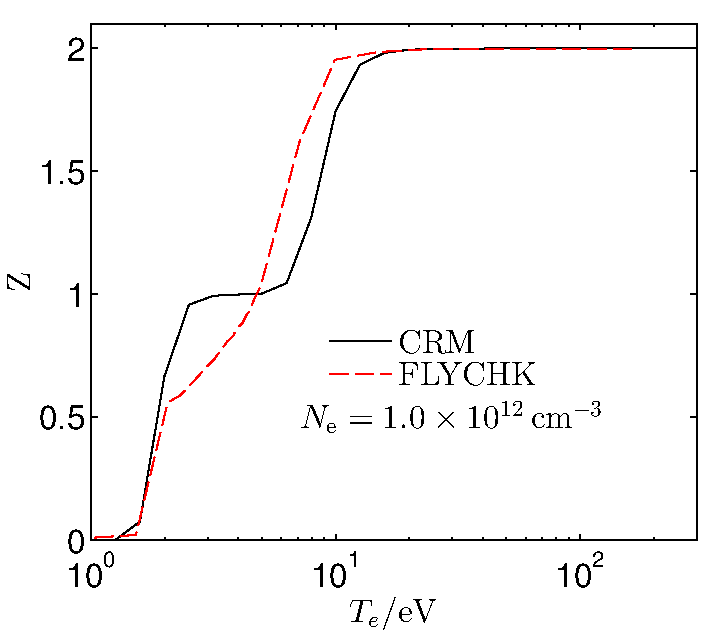
\includegraphics[width=0.5\textwidth]{ZvsTe-spec-Ne-1_0E2.pdf}
  \caption{氦等离子体稳态时平均电荷数与电子温度 $T_{\rm e}$ 的关系。实线为本文碰撞辐射模型计算结果,虚线为 FLYCHK 的计算结果。图片修改自 \onlinecite{xie:wlxb}。}
  \label{fig:chap03:ZvsTe}
\end{figure}

做为对比,图 \ref{fig:chap03:ZvsTe} 给出了在电子密度 $N_{\rm e}=1.0\times10^{12}\,{\rm cm}^{-3}$ 条件下,当达到稳态时, 本文碰撞辐射模型与 FLYCHK\cite{FLYCHK,FLYCHK:url} 代码计算的平均电荷数 $\overline{Z}$ 随 $T_{\rm e}$ 的变化曲线。由图可知,当 $T_{\rm e}>10\,{\rm eV}$ 时,本论文模型与 FLYCHK 的计算结果可以吻合,等离子体中的氦原子已经几乎达到完全电离的状态。两模型的计算结果在 $T_{\rm e}=2\,{\rm eV}-10\,{\rm eV}$ 范围内有最大约 $30\%$ 的误差,这主要是因为两者使用的电子碰撞截面不同造成的。当 $T_{\rm e}$ 在跃迁能量附近时,碰撞反应截面具有比较复杂的行为,无论理论计算还是实验测量都难以获得满意的结果 \cite{Ralchenko2008603},本论文模型计算结果在 $T_{\rm e}=2.5\,{\rm eV}-6\,{\rm eV}$ 的阶梯也可能是由所使用的碰撞截面拟合公式较差的精度造成的。

%\section{SUNIST 氦原子碰撞辐射模型研究}
\section{氦原子碰撞辐射模型的研究}

%\subsection{能级数密度计算结果}


\subsection{各激发态能级的主要产生过程研究}
\label{sec:main-inflow}

通过各能级的主要产生与损失过程可研究 SUNIST 参数下的氦放电等离子体原子的反应特点,如图 $\ref{fig:chap03:main-inflow}$ 所示为超过各能级总产生速率 $10\%$ 的粒子流示意图。因为 SUNIST 主要使用 $n=4$ 能级的原子谱线进行诊断,$n=4$ 各能级的粒子产生流单独画出,而将 $n=3$ 和 $n\ge5$ 的能级分别合并为 $3^1{\rm L}$、$3^3{\rm L}$ 与 $^1hl$、$^3hl$ 能级。

\begin{figure}
    \centering
%    \begin{subfigure}{0.45\columnwidth}
%        \fbox{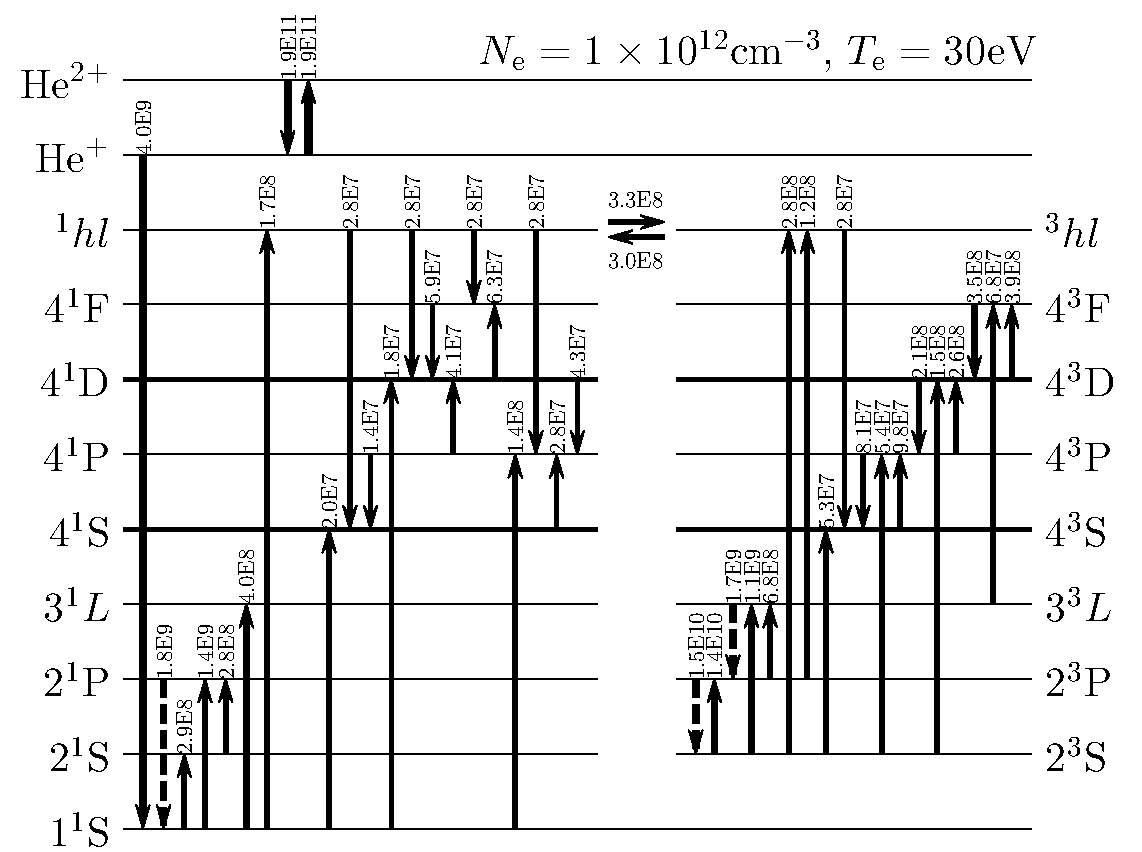
\includegraphics[width=\columnwidth]{Ne1E12_Te30_1e7cm-3s-1.pdf}}
%        \caption{}%
%        \label{fig:chap03:main-inflow:1}
%    \end{subfigure}
%    \hspace{0.05\textwidth}
%    \begin{subfigure}{0.45\columnwidth}
%        \fbox{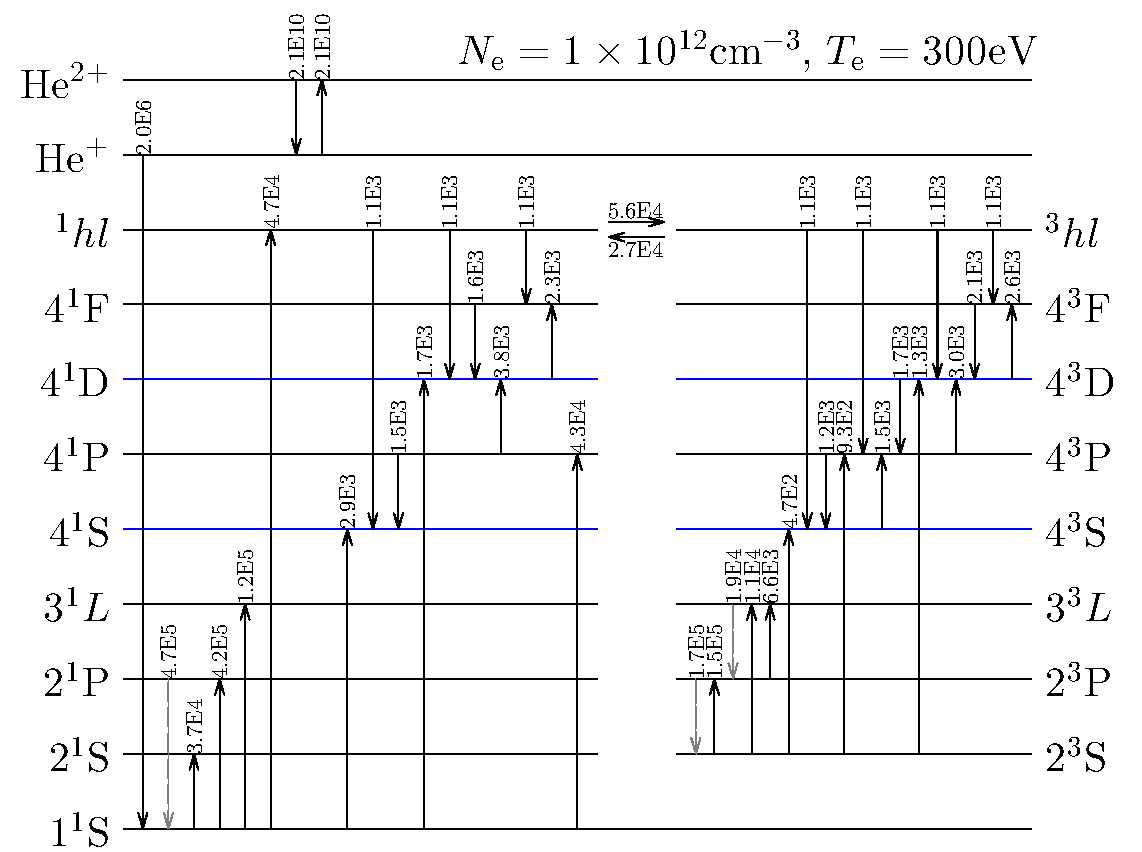
\includegraphics[width=\columnwidth]{Ne1E12_Te300_1e7cm-3s-1.pdf}}
%        \caption{}%
%        \label{fig:chap03:main-inflow:2}
%    \end{subfigure}\\
%    \begin{subfigure}{0.45\columnwidth}
%        \fbox{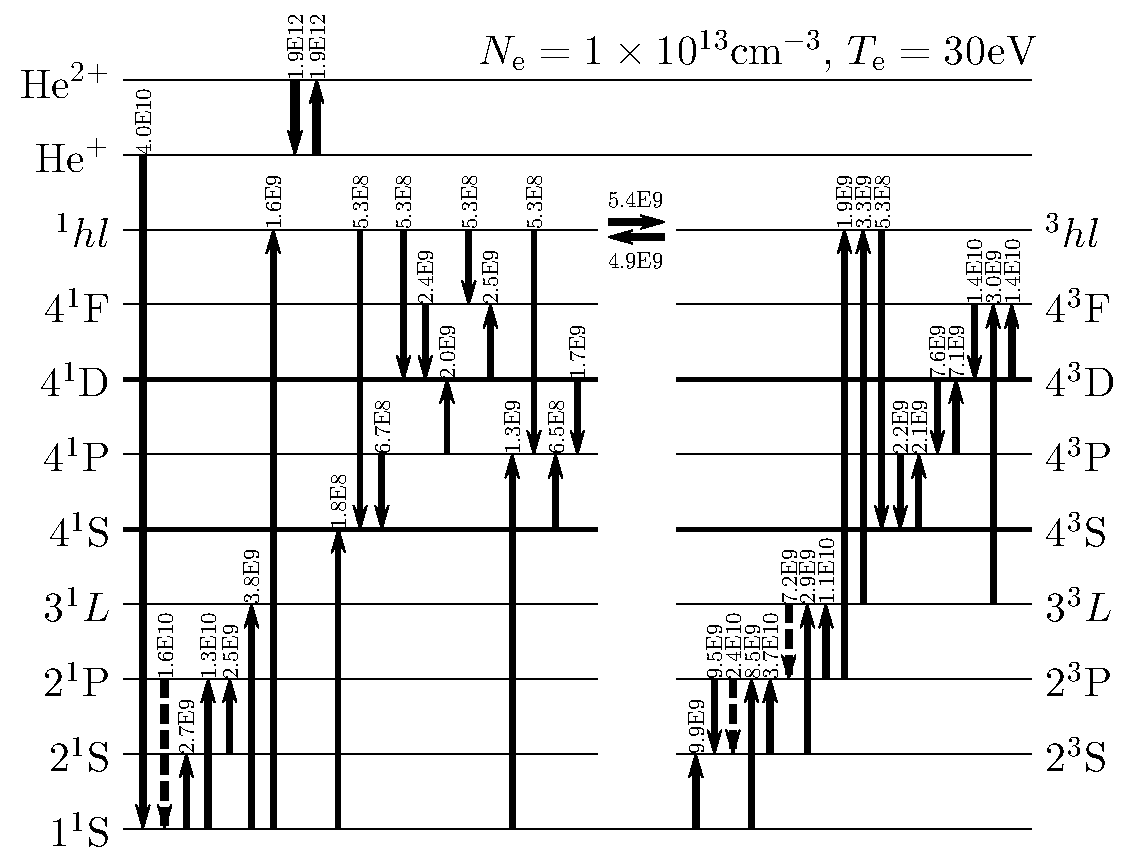
\includegraphics[width=\columnwidth]{Ne1E13_Te30_1e7cm-3s-1.pdf}}
%        \caption{}%
%        \label{fig:chap03:main-inflow:3}
%    \end{subfigure}
%    \hspace{0.05\textwidth}
%    \begin{subfigure}{0.45\columnwidth}
%        \fbox{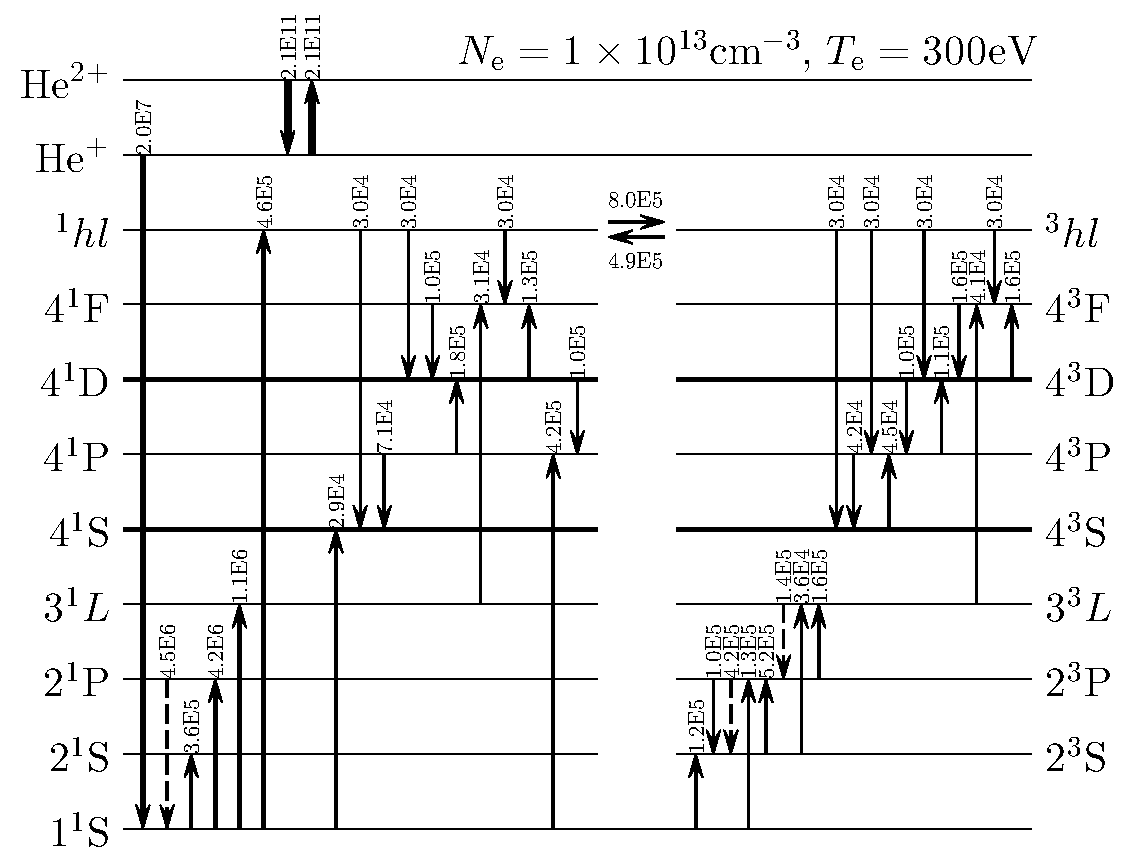
\includegraphics[width=\columnwidth]{Ne1E13_Te300_1e7cm-3s-1.pdf}}
%        \caption{}%
%        \label{fig:chap03:main-inflow:4}
%    \end{subfigure}
    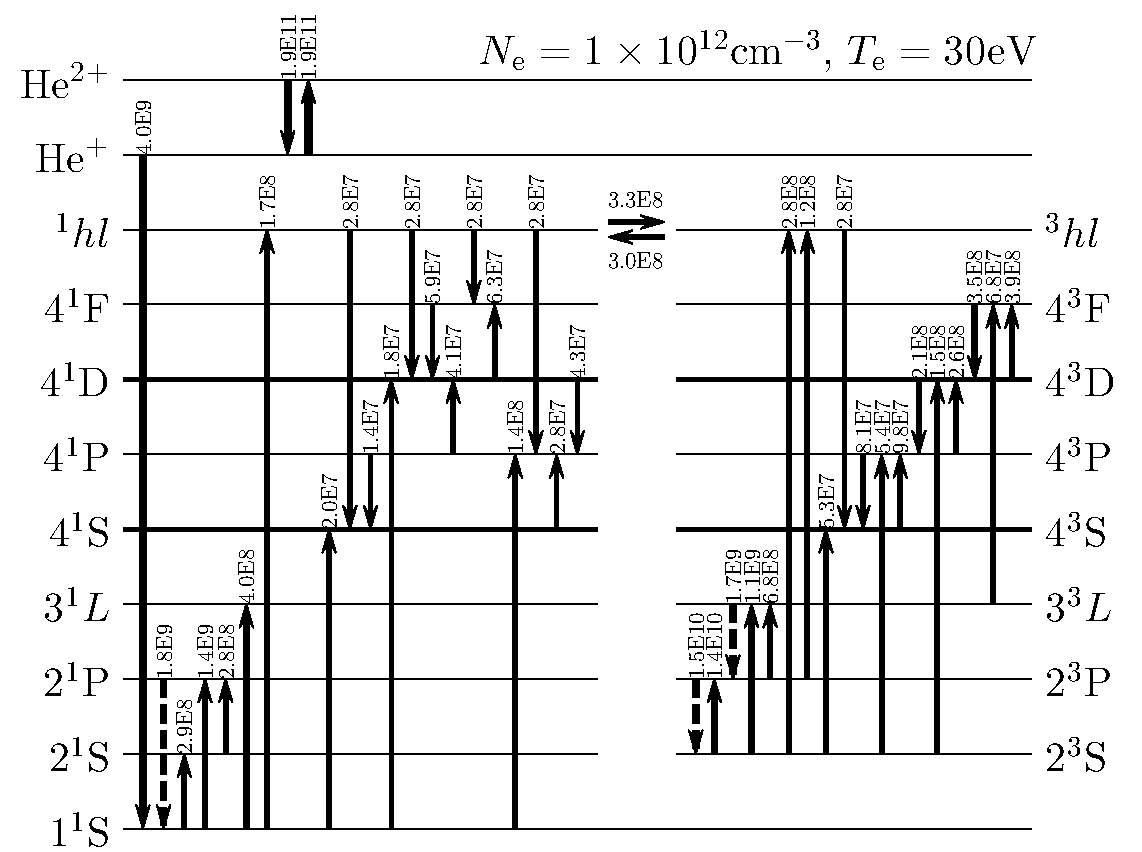
\includegraphics[width=0.8\textwidth]{Ne1E12_Te30_1e7cm-3s-1.pdf}
    \caption{根据碰撞辐射模型结果,
    %不同 $T_{\rm e}$ 和 $N_{\rm e}$ 参数下,
    各能级的主要产生(占比大于该能级总产生速率的 $10\%$)过程。%其中,主量子数 $n\geq 5$ 的能级合并为一个高能级 $hl$。
    其中,虚线箭头为自发辐射跃迁过程,实线箭头为碰撞跃迁过程。}%
    \label{fig:chap03:main-inflow}
\end{figure}

在 $N_{\rm e}=1\times10^{12}\,{\rm cm}^{-3},\,T_{\rm e}=30\,{\rm eV}$ 条件下,$4^1{\rm S}$ 与 $4^1{\rm D}$ 能级的主要产生粒子流来自基态激发、自旋单态高能级 $^1hl$ 退激发以及来自 $n=4$ 的相邻能级的粒子重分配(redistribution),对于$4^3{\rm S}$ 与 $4^3{\rm D}$ 能级,亚稳态 $2^3{\rm S}$ 则取代基态能级,成为主要产生过程的来源之一。另外,对于普通激发态能级,电子碰撞电离与复合过程的产生粒子流不会超过总产生速率流量的10\%。

基态能级粒子的产生主要来自 ${\rm He}^+$ 的复合过程(超过 $80\%$),$2^1{\rm P}$ 能级的共振线辐射也贡献了约 $20\%$ 的粒子产生流,基态的损失则主要由电子碰撞激发至更高能级粒子贡献。亚稳态 $2^3{\rm S}$ 粒子一部分来自基态的自旋变化激发过程,一部分来自其它自旋三重态能级的退激发过程产生。高激发态能级($n\ge5$)粒子则在氦离子与 $n\le4$ 激发态之间起到了桥梁作用。由第 \ref{sec:FLYCHK-compare} 节,氦等离子体的电离率很高,${\rm He}^+$ 与 ${\rm He}^{2+}$ 离子之间的电离与复合过程占了最主要的反应过程部分。

其他 $T_{\rm e}$ 和 $N_{\rm e}$ 条件下的情况与此类似(附录 \ref{appendix:main-inflow}),只是在更高电子密度情况下,基态的电子碰撞激发至 $2^3{\rm S}$ 过程显得更为明显。

\subsection{速率系数不确定性到激发态数密度计算误差传递的研究}
\label{sec:chap04:uncertainty-transport}

碰撞辐射模型中使用的速率系数任何不确定性的存在,都会传递给模型对能级数密度的计算。模型中包含着众多能级粒子与复杂的反应过程,并且相互耦合,现阶段缺乏直接有效的手段对速率系数不确定性的影响进行估计。通常的做法是,对某反应过程的速率系数进行相应扰动,重新计算碰撞辐射模型的速率方程,以观察扰动后的计算结果相对原来的变化\cite{Andrew2000PPCFSensitivity}。

%基于激发态主要产生过程的分析,对于普通激发态(如 $n=4$),其电子碰撞电离与复合过程都不会高于该能级总损失或产生速率的 $10\%$。则在准稳态情况下,对于 $p$ 激发态能级,如下的方程可以成立:
%\begin{equation}
%N_{\rm e}\sum_{i\ne p}C_{ip}N_i=N_{\rm e}N_p\sum_{i\ne p}C_{pi}+N_p\sum_{i<p}A_{pi}
%\label{eq:error:rateequation}
%\end{equation}
%其中 $i$ 可以通过电子碰撞激发或退激发过程可以直接与 $p$ 能级联系的激发态能级粒子。$C_{ip}$、$C_{pi}$ 与 $A_{pi}$ 分别表示电子碰撞产生、损失与自发退激辐射速率系数。而 $i$ 与 $p$ 能级的粒子数密度分别记为$N_i$ 和 $N_p$。由方程 (\ref{eq:error:rateequation}) 可以得出:
%\begin{equation}
%N_p=\frac{N_{\rm e}\sum_{i\ne p}C_{ip}N_i}{N_{\rm e}\sum_{i\ne p}C_{pi}+\sum_{i<p}A_{pi}}
%\label{eq:error:Np}
%\end{equation}
%估计由速率系数不确定性 $s(C_{ip})$ 对 $p$ 能级粒子数引起的最大相对误差\cite{YuChangxuan:book}。 则:
%\begin{eqnarray}
%s_{N_p}=\frac{{\rm d}N_p}{N_p} = s\left(N_{\rm e}\sum_{i\ne p}C_{ip}N_i\right) + s\left(N_{\rm e}\sum_{i\ne p}C_{pi}+\sum_{i<p}A_{pi}\right)% \nonumber \\
%% & = & \frac{}{} + \frac{}{}
%\label{eq:error:EqOrig}
%\end{eqnarray}
%经过推导(附录 \ref{appendix:error-propagate}),可以得出:
%\begin{eqnarray}
%s_{N_p}=E_{jp}\cdot s(C_{jp})=2\frac{f_{jp}}{F_{p,{\rm in}}}s(C_{jp})
%\label{eq:error:Propagation}
%\end{eqnarray}
%其中
%\begin{eqnarray}
%E_{jp}=2\frac{f_{jp}}{F_{p,{\rm in}}}
%\label{eq:error:Propagation}
%\end{eqnarray}
%为 $j\to p$ 反应过程的速率系数不确定性传递函数,其中 $f_{jp}$ 与 $F_{p,{\rm in}}$ 分别表示 $j\to p$ 能级粒子的产生速率与 $p$ 能级的总粒子产生速率。

普通激发态(如 SUNIST 使用的 $n=4$ 能级)具有可以用来进行谱线诊断的谱线辐射,碰撞辐射模型对这些能级的计算精度是我们所主要关注的。因此,在速率系数不确定性传递的推导过程中,我们主要关注这些激发态能级的数密度。为了简化问题,在所有的感兴趣能级产生过程中,考虑同时只有其中某一个过程 $j\to p$ 的速率系数 $C_{jp}$ 具有不确定性\cite{Andrew2000PPCFSensitivity},研究其对感兴趣能级粒子数密度 $N_p$ 引起的相对误差。

由第 \ref{sec:main-inflow} 节对能级主要产生过程的分析我们可以得到,对于普通激发态能级,无论是电子碰撞复合产生过程,还是电离过程的数密度损失速率,都不足以超过其产生或损失总粒子数速率。所以,对于准稳态情况下的等离子体,$p$ 能级离子的总产生速率与总损失速率相等,则:
\begin{equation}
N_{\rm e}\sum_{i\ne p}C_{ip}N_i=N_{\rm e}N_p\sum_{i\ne p}C_{pi}+N_p\sum_{i<p}A_{pi}
\label{eq:appendix:error:rateequation}
\end{equation}
其中 $i$ 表示与 $p$ 能级发生电子碰撞激发、退激发或自发辐射过程的能级;$C_{ip}$、$C_{pi}$ 与 $A_{pi}$ 分别为 $p$ 能级的电子碰撞产生,损失与自发辐射速率系数;而电子密度、$i$ 能级与 $p$ 能级的粒子数密度分别记为 $N_{\rm e}$、$N_i$ 与 $N_p$。

从式 (\ref{eq:appendix:error:rateequation}) 可以解出 $N_p$:
\begin{equation}
N_p=\frac{N_{\rm e}\sum_{i\ne p}C_{ip}N_i}{N_{\rm e}\sum_{i\ne p}C_{pi}+\sum_{i<p}A_{pi}}
\label{eq:appendix:error:Np}
\end{equation}
这里,对于速率系数不确定性引起的 $N_p$ 相对误差,我们计入最大估计值\cite{YuChangxuan:book}:
\begin{eqnarray}
s_{N_p}=\frac{{\rm d}N_p}{N_p}& = &s\left(N_{\rm e}\sum_{i\ne p}C_{ip}N_i\right) + s\left(N_{\rm e}\sum_{i\ne p}C_{pi}+\sum_{i<p}A_{pi}\right)% \nonumber \\
% & = & \frac{}{} + \frac{}{}
\label{eq:appendix:error:EqOrig}
\end{eqnarray}
对于 $n=4$ 普通激发态,自发辐射能级产生或损失过程的速率小于总产生或损失速率的 $10\%$,同时自发辐射速率系数可以精确得到\cite{NISTdatabase},在式 (\ref{eq:appendix:error:EqOrig}) 右侧第二项中,忽略自发辐射过程的影响,则
\begin{eqnarray}
s_{N_p}& = &s\left(N_{\rm e}\sum_{i\ne p}C_{ip}N_i\right) + s\left(N_{\rm e}\sum_{i\ne p}C_{pi}\right) \nonumber\\
            & \simeq & \frac{{\rm d}F_{p,{\rm in}}}{F_{p,{\rm in}}} + \frac{{\rm d}F_{p,{\rm out}}}{F_{p,{\rm out}}}
\label{eq:appendix:error:EqIgnoreAqi}
\end{eqnarray}
其中 $F_{p,{\rm in}}=N_{\rm e}\sum C_{ip}N_i$ 与 $F_{p,{\rm out}}=N_{\rm e}N_p\sum C_{pi}$ 分别为 $p$ 能级的电子碰撞产生与损失总速率。根据精细平衡\cite{Lieberman2005-book} 原则,认为电子碰撞激发与退激发具有相同的相对误差是合理的,则 $N_p$ 的相对误差可以写为:
\begin{eqnarray}
s_{N_p} \simeq 2\left(\frac{{\rm d}F_{p,{\rm in}}}{F_{p,{\rm in}}}\right)
\simeq 2\left(\frac{{\rm d}F_{p,{\rm out}}}{F_{p,{\rm out}}}\right)
\label{eq:appendix:error:EqFinal}
\end{eqnarray}
为了简化,此时仅考虑 $j\to p$ 过程的速率系数具有为 $s(C_{jp})={\rm d}C_{jp}/C_{jp}$ 的不确定性\cite{Andrew2000PPCFSensitivity},则 $p$ 能级的总产生速率相对误差为:
\begin{eqnarray}
{\rm d}F_{p,{\rm in}}={\rm d}f_{jp}&=&{\rm d}\left(N_{\rm e}N_jC_{jp}\right)\nonumber\\
&=&N_{\rm e}C_{jp}N_j\frac{{\rm d}C_{jp}}{C_{jp}}+N_{\rm e}C_{jp}N_j\frac{{\rm d}N_j}{N_j}\nonumber\\
&=&f_{jp}s\left(C_{jp}\right)+f_{jp}s\left(N_j\right)
\label{eq:appendix:error:dFin}
\end{eqnarray}
其中 $j\to p$ 过程的粒子反应速率记为 $f_{jp}$。根据式 (\ref{eq:appendix:error:EqFinal}),$s(N_j)$ 可以重写为
\begin{eqnarray}
s(N_j)\simeq 2\left(\frac{{\rm d}F_{j,{\rm out}}}{F_{j,{\rm out}}}\right)
\label{eq:appendix:error:sigmaNjOrig}
\end{eqnarray}
碰撞辐射模型的反应速率方程处于准稳态,则 $p$ 能级的粒子数总产生速率与总损失速率相等,所以
\begin{eqnarray}
F_{j,{\rm out}}&=&F_{j,{\rm in}}
\label{eq:appendix:error:FjinANDdFjin}
\end{eqnarray}
当速率系数的不确定性引起粒子数速率变化时,则有
\begin{eqnarray}
{\rm d}F_{j,{\rm out}}&\simeq&{\rm d}f_{jp}
\label{eq:appendix:error:dFjinANDdFjin}
\end{eqnarray}
那么式 (\ref{eq:appendix:error:sigmaNjOrig}) 即可以写为:
\begin{eqnarray}
s(N_j)\simeq 2\left(\frac{{\rm d}f_{jp}}{F_{j,{\rm in}}}\right)
\label{eq:appendix:error:sigmaNj}
\end{eqnarray}
将式 (\ref{eq:appendix:error:sigmaNj}) 代入式 (\ref{eq:appendix:error:dFin}),可以得到:
\begin{eqnarray}
{\rm d}f_{jp}=f_{jp}s\left(C_{jp}\right)+2f_{jp}\left(\frac{{\rm d}f_{jp}}{F_{j,{\rm in}}}\right)
\label{eq:appendix:error:dfjpEq}
\end{eqnarray}
则 ${\rm d}f_{jp}$ 可以简化为:
\begin{eqnarray}
{\rm d}f_{jp}=\left(1-\frac{2}{F_{j,{\rm in}}}\right)^{-1}f_{jp}s(C_{jp})
\label{eq:appendix:error:dfjp}
\end{eqnarray}
根据式 (\ref{eq:appendix:error:EqFinal})、(\ref{eq:appendix:error:dFin}) 与 (\ref{eq:appendix:error:dfjp}),我们可以得到速率系数不确定性 $s(C_{jp})$ 引起 $p$ 激发态能级粒子数 $N_p$ 的相对误差 $s_{N_p}$ 为
\begin{eqnarray}
s_{N_p}=E_{jp}s(C_{jp})=2\left(1-\frac{2}{F_{j,{\rm in}}}\right)^{-1}\frac{f_{jp}}{F_{p,{\rm in}}}s(C_{jp})
\label{eq:appendix:error:Propagation}
\end{eqnarray}
其中
\begin{eqnarray}
E_{jp}=2\left(1-\frac{2}{F_{j,{\rm in}}}\right)^{-1}\frac{f_{jp}}{F_{p,{\rm in}}}
\simeq 2\frac{f_{jp}}{F_{p,{\rm in}}}
\label{eq:appendix:error:PropagationCoeff}
\end{eqnarray}
为\emph{速率系数不确定性传递函数}(the uncertainty propagation coefficient),$F_{j,{\rm in}}$、$f_{jp}$ 与 $F_{p,{\rm in}}$ 可以从碰撞辐射模型的计算结果直接计算获得。在式(\ref{eq:appendix:error:PropagationCoeff}) 中假设
\begin{eqnarray}
F_{j,{\rm in}}\gg 2
\label{eq:appendix:error:FjinLargerThan2}
\end{eqnarray}
总是成立。

然而,式 (\ref{eq:appendix:error:Propagation}) 仅可用来计算与 $p$ 能级直接相关的反应过程速率系数不确定性的传递。具 SUNIST 参数的氦放电等离子体的电离度 $\sim 1$,其离子数含量非常之高,则 ${\rm He}^+$ 到基态能级 $1^1{\rm S}$ 的速率系数不确定性会通过基态的二级反应过程(secondary stepwise process)对感兴趣能级的粒子数产生影响,而 ${\rm He}^+$ 与 ${\rm He}^{2+}$ 之间的电离与复合过程速率系数则会通过三级反应过程,以及其他可以对基态能级粒子数总产生或消失速率产生影响的反应过程都会对对 $p$ 能级粒子数产生影响。

对于二级反应过程,$N_1$ 的粒子数密度会发生变化,而基态到 $p$ 的速率系数 $C_{1p}$ 不变。所以:
\begin{eqnarray}
{\rm d}f_{1p}=N_{\rm e}C_{1p}{\rm d}N_1\simeq N_{\rm e}C_{1p}N_1\frac{{\rm d}N_1}{N_1}=f_{1p}s(N_1)
\label{eq:appendix:error:secondary:df1p}
\end{eqnarray}
联立式 (\ref{eq:appendix:error:EqFinal})、(\ref{eq:appendix:error:dFin})、(\ref{eq:appendix:error:Propagation}) 与 (\ref{eq:appendix:error:secondary:df1p}),可以得到:
\begin{eqnarray}
s_{N_p}&=&2\frac{f_{1p}}{F_{p,{\rm in}}}s(N_1)
=2\frac{f_{1p}}{F_{p,{\rm in}}}E_{j1}s(C_{j1})\nonumber \\
&=&E_{j1p}s(C_{j1})
\label{eq:appendix:error:secondary:sigmaNp}
\end{eqnarray}
其中 $E_{j1}$ 与式 (\ref{eq:appendix:error:PropagationCoeff}) 具有相同的形式。

与上面二级反应过程相同的推导,$s(C_{{\rm He}^{2+}{\rm He}^+})$ 与 $s(C_{{\rm He}^+{\rm He}^{2+}})$ 到 $s_{N_p}$ 的传递可以分别写为:
\begin{eqnarray}
s_{N_p}&=&2^2\cdot\frac{f_{1p}}{F_{p,{\rm in}}}%s(N_1)
\cdot
\frac{f_{{\rm He}^+1}}{F_{1,{\rm in}}}
\cdot
E_{{\rm He}^{2+}{\rm He}^+}s(C_{{\rm He}^{2+}{\rm He}^+})\nonumber\\
&=&E_{{\rm He}^{2+}{\rm He}^+1p}s(C_{{\rm He}^{2+}{\rm He}^+})
\label{eq:appendix:error:HeII:sigmaNp}
\end{eqnarray}
与
\begin{eqnarray}
s_{N_p}&=&2^3\cdot\frac{f_{1p}}{F_{p,{\rm in}}}%s(N_1)
\cdot
\frac{f_{{\rm He}^+1}}{F_{1,{\rm in}}}
\cdot
\frac{f_{{\rm He}^{2+}{\rm He}^+}}{F_{{\rm He}^+,{\rm in}}}
\cdot
E_{{\rm He}^+{\rm He}^{2+}}s(C_{{\rm He}^+{\rm He}^{2+}})\nonumber\\
&=&E_{{\rm He}^+{\rm He}^{2+}{\rm He}^+1p}s(C_{{\rm He}^+{\rm He}^{2+}})
\label{eq:appendix:error:HeIII:sigmaNp}
\end{eqnarray}

最后,我们可以将速率系数不确定性通过 $i\to j\to\cdots\to q\to p$ 多级反应过程传递给 $s_{N_p}$ 的不确定性传递函数写为:
\begin{eqnarray}
E_{ij\cdots qp}=E_{qp}E_{.q}\cdots E_{j.}E_{i\to j}
\label{eq:appendix:error:MPDcoefficient}
\end{eqnarray}
附录 \ref{appendix:error-propagate} 给出本工作使用的碰撞辐射模型中,多种反应速率系数的不确定性传递函数的计算结果。

速率系数不确定性传递函数表示的意义为:当只有反应过程 $j\to p$ 的速率系数存在不确定性时,其相对误差 $s(C_{jp})$ 与由此引起的碰撞辐射模型对 $p$ 能级数密度计算的相对误差 $s_{N_p}$ 之比。其中,某一反应过程占感兴趣能级总粒子产生速率的比重越大,其速率系数不确定性的影响越明显;在准稳态条件下,其逆过程的粒子反应速率会有同等量级的变化,在误差传递函数中则以两倍的系数体现逆过程的影响。据此,可以对速率系数的准确度提出具体要求。可见,碰撞辐射模型对第 \ref{sec:main-inflow} 节中我们得到的激发态主要产生过程的速率系数精度具有较高的要求。

\begin{figure}%[H]
  \centering
  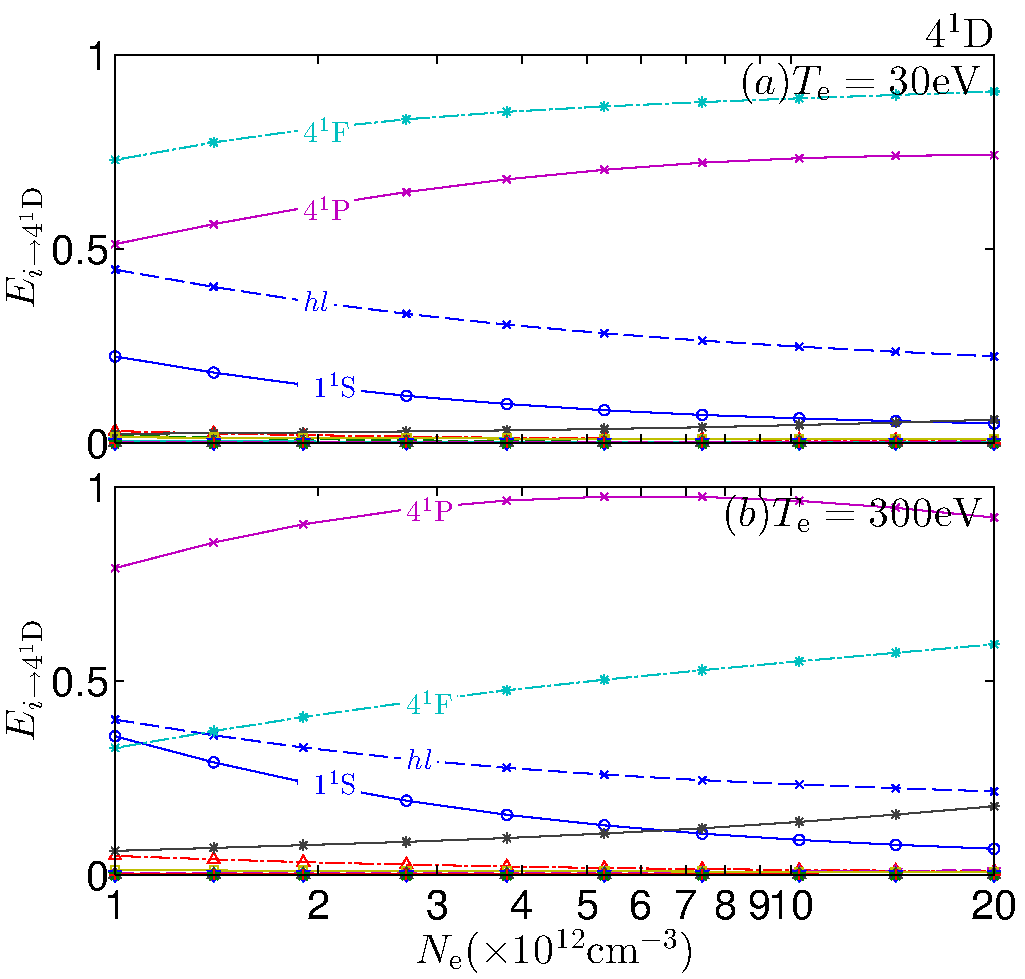
\includegraphics[width=0.6\textwidth]{41D-error-propagation-coefficient.pdf}
  \caption{氦原子 $4^1{\rm D}$ 能级产生过程的速率系数不确定性传递函数}
  \label{fig:chap03:41D-error-propgation-function}
\end{figure}


以 $4^1{\rm D}$ 能级为例,其产生过程的速率系数不确定性传递函数在不同 $T_{\rm e}$ 条件下随电子密度的变化结果在图 \ref{fig:chap03:41D-error-propgation-function} 中画出。在 $T_{\rm e}=30\,{\rm eV}$ 时,来自相同主量子数的相邻能级($4^1{\rm F}$ 和 $4^1{\rm P}$)跃迁产生速率系数不确定性的传递函数随着电子密度的增大而增长,$4^1{\rm F}$ 能级的跃迁速率系数不确定性传递函数甚至会达到 $1$,这意味着 $4^1{\rm F}\to 4^1{\rm D}$ 过程速率系数的不确定性会以相同的量级体现在 $4^1{\rm D}$ 粒子数密度的计算结果上。高能级 $hl$ 与基态能级的不确定性传递函数分别低于 $0.5$ 和 $0.2$,并且随着电子密度的增大而减弱。当电子温度较高时,$4^1{\rm D}$ 各产生过程的速率系数不确定性传递函数具有与电子温度较低时相同的趋势,不过来自 $4^1{\rm F}$ 能级过程的速率系数不确定性传递函数降低到了 $0.5$ 左右,而来自 $4^1{\rm P}$ 过程的速率系数不确定性传递函数则增长到了 $1$ 左右。

\begin{figure}%[H]
  \centering
  \begin{overpic}[width=0.6\textwidth]{41D-error-propagation.pdf}
    \put(-3,16){\rotatebox{90}{\mbox{\colorbox{white}{相对误差 ($\%$)}}}}
    \put(-3,58){\rotatebox{90}{\mbox{\colorbox{white}{相对误差 ($\%$)}}}}
  \end{overpic}
%  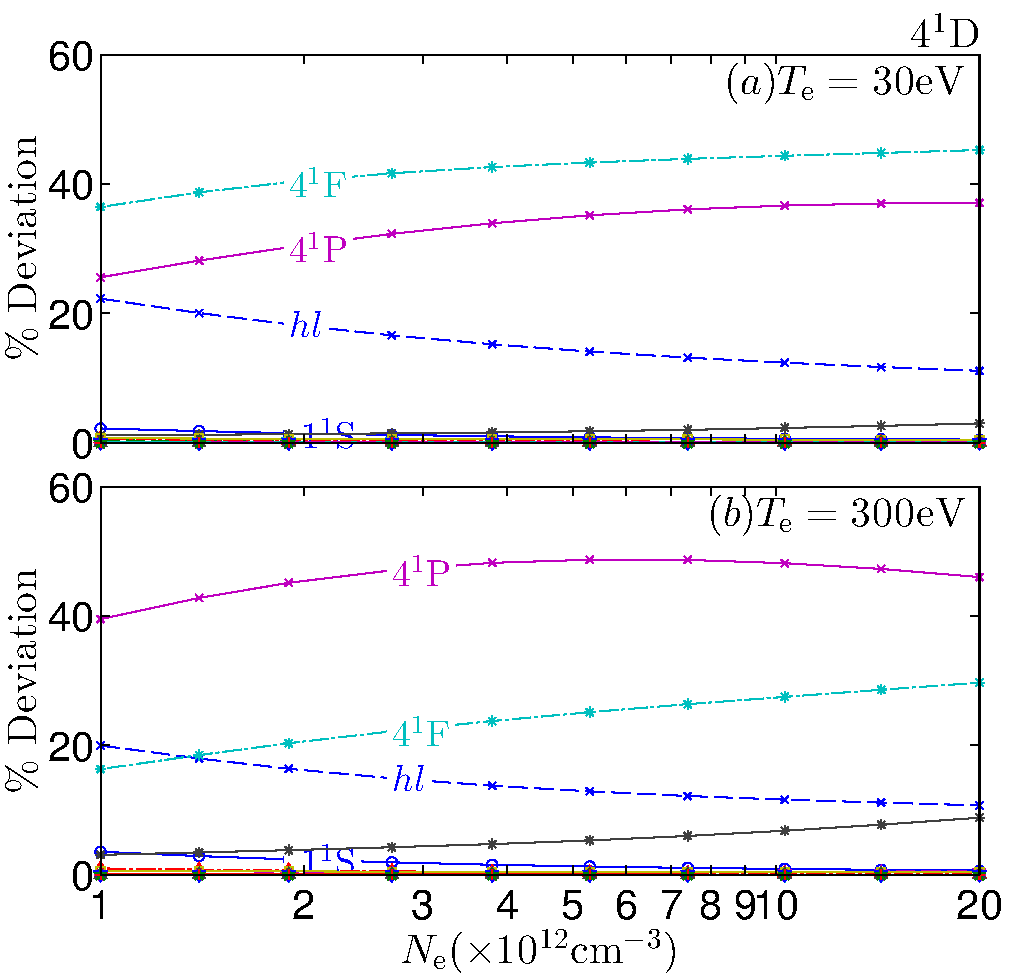
\includegraphics[width=0.6\textwidth]{41D-error-propagation.pdf}
  \caption{氦原子 $4^1{\rm D}$ 能级产生过程的不确定性传递结果}
  \label{fig:chap03:41D-error-propgation-result}
\end{figure}

如图 \ref{fig:chap03:41D-error-propgation-result} 所示,以表 \ref{tab:chap03:rate-uncertainty} 所列各过程的速率系数不确定性为原始数据,分别计算了这些速率系数的不确定性所引起的碰撞辐射模型对 $4^1{\rm D}$ 能级数密度的计算相对误差。由于基态激发速率系数的精度较高,其激发过程的速率系数误差影响可以忽略,而高能级 $hl$ 的速率系数总影响在低于 $20\%$ 的范围内,考虑到这是 $n\ge5$ 的众多能级的总贡献,当只有来自 $n\ge5$ 单一能级的反应过程速率系数具有不确定性时,或这些能级的不确定性均具有不确定性,但不同过程存在正负误差时,高能级产生过程的速率系数不确定性影响可以相互抵消。

在温度较低时,来自相邻能级 $4^1{\rm P}$ 和 $4^1{\rm F}$ 的产生过程速率系数均会带来约 $40\%$ 的相对误差;当温度较高时,$4^1{\rm P}$ 起始过程带来的影响会增加到 $40\%$ 以上,$4^1{\rm F}$ 的影响会降低,但仍保持在 $20\%$ 上下的范围。这说明碰撞辐射模型对相同主量子数能级粒子之间的数密度重新分配过程的速率系数要求很高,但由于实验和理论上的限制,这些速率系数的不确定性精度受到限制\cite{Bray2000:He-data,Delabie2010:consistency},要提高碰撞辐射模型的计算精度,在速率系数的实验、理论上仍需进一步积累\cite{Summers:IAEAdatarequirement}。

由于碰撞辐射模型中多种粒子复杂的反应过程相互耦合,目前尚无手段对反应速率系数不确定性到激发态粒子数密度计算误差的传递进行简洁而有效的计算。前面提到,Y. Andrew 等人\cite{Andrew2000PPCFSensitivity}采用扰动法,将某反应速率系数进行扰动后,重新对碰撞辐射模型进行计算,以获得对速率系数所做的扰动带来的影响。这种对每个速率系数进行扰动并在不同的 $T_{\rm e}$ 和 $N_{\rm e}$ 组合条件下重新解反应速率方程的过程繁复耗时,且不直观,物理意义不明确。我们引入的不确定性传递函数可以直观的体现感兴趣过程的速率系数不确定性到粒子数密度计算结果的影响,且物理意义明确。有助于快速定位对碰撞辐射模型计算产生主要影响的反应过程,并对此做出相应的分析和处理。

另外,通过附录 \ref{appendix:error-propagate} 给出的结果,还可以分析如 ${\rm He}^+$ 复合至基态能级 $1^1{\rm S}$ 的速率系数不确定性通过两次反应过程对如 $n=4$ 的普通激发态能级数密度产生影响的不确定性传递函数,甚至是通过三级或多级反应过程的不确定性传递函数。

\subsection{碰撞辐射模型中包含的能级对计算结果影响的研究}
\label{sec:chap03:maxn-in-crm}

碰撞辐射模型中包含的能级与反应过程的多少对感兴趣能级粒子数密度的计算会产生影响。我们知道,由于反应过程速率系数不确定性的存在,模型包含更多数目的能级和反应过程并不能如以前人们所预期的那样可以得到更高精度的粒子数密度计算结果。本节主要研究包含到最高能级主量子数 $\max n$ 至什么程度即可以满足对计算精度的要求。

由于氦原子 $n\le4$ 能级的电子碰撞电离与它们之间的跃迁截面数据具有较高的精度,对于 SUNIST 参数下的氦等离子体,我们分别计算在碰撞辐射模型最高包含至 $\max n=5, 6, 7 \cdots$ 时能级粒子数密度的计算结果与最高包含至 $\max n-1$ 时计算结果的相对误差:
\begin{equation}
\Delta N_i^{\max n}=100\%\times\frac{N_i^{\max n}-N_i^{\max n-1}}{N_i^{\max n-1}}
\label{eq:chap03:rel-diff-maxn}
\end{equation}
其中,$N_i^{\max n}$ 与 $N_i^{\max n-1}$ 分别为碰撞辐射模型包含最高至主量子数为 $\max n$ 和  $\max n-1$ 时的 $i$ 能级粒子数密度计算结果。

\begin{figure}%[H]
    \centering
    \begin{subfigure}{0.47\textwidth}
        %\begin{overpic}[width=\textwidth]{levelabun-13-41S-Ne5_0E12-ss-reldiff-manx4to7.pdf}
        %    \put(-2,40){\rotatebox{90}{\colorbox{white}{$\Delta_{N_{4^1{\rm S}}}^{\max n}$ ($\%$)}}}
        %\end{overpic}
        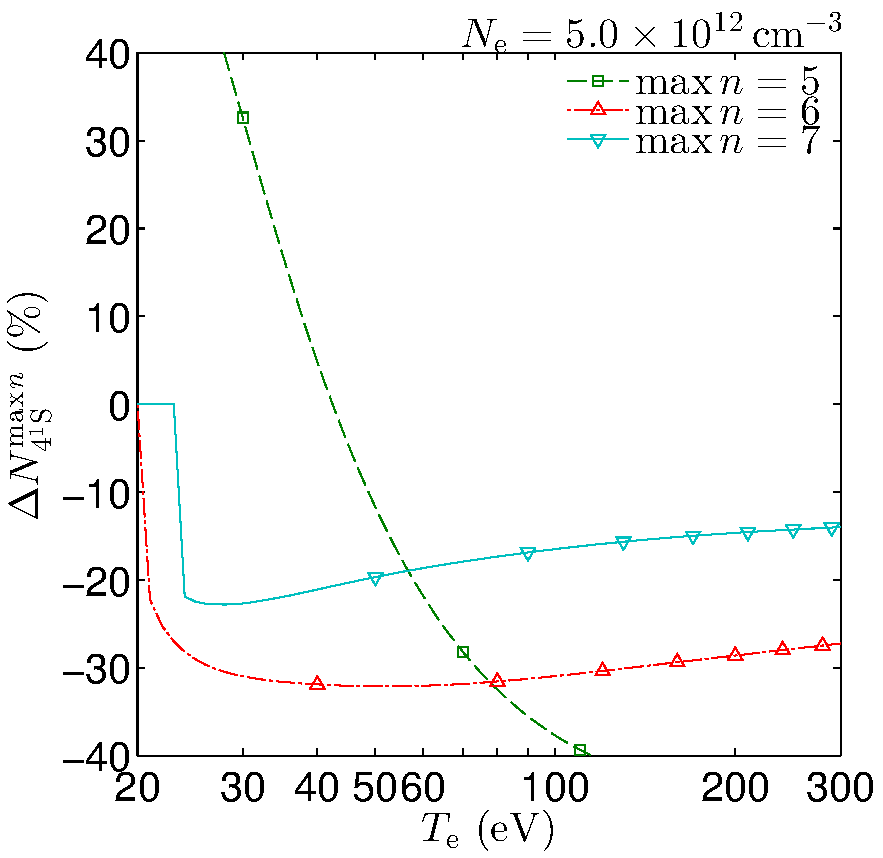
\includegraphics[width=\textwidth]{levelabun-13-41S-Ne5_0E12-ss-reldiff-manx4to7.pdf}
        \caption{随 $T_{\rm e}$ 的变化}%
        \label{fig:chap03:41S-levelabun-reldiff:1}
    \end{subfigure}
    %\hspace{0.05\textwidth}
    \begin{subfigure}{0.47\columnwidth}
        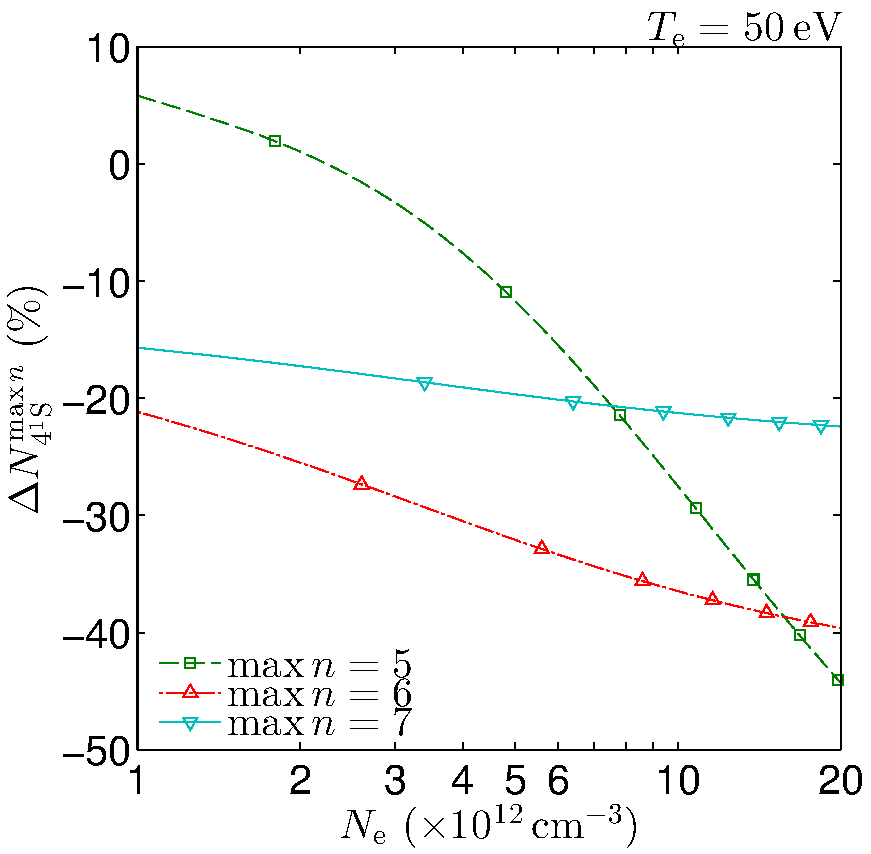
\includegraphics[width=\columnwidth]{levelabun-13-41S-Te50-ss-reldiff-manx4to7.pdf}
        \caption{随 $N_{\rm e}$ 的变化}%
        \label{fig:chap03:41S-levelabun-reldiff:2}
    \end{subfigure}
    \caption{包含至不同最高主量子数能级时,氦原子 $4^1{\rm S}$ 能级数密度计算的相对误差。}%
    \label{fig:chap03:41S-levelabun-reldiff}
\end{figure}

\begin{figure}%[H]
  \centering
  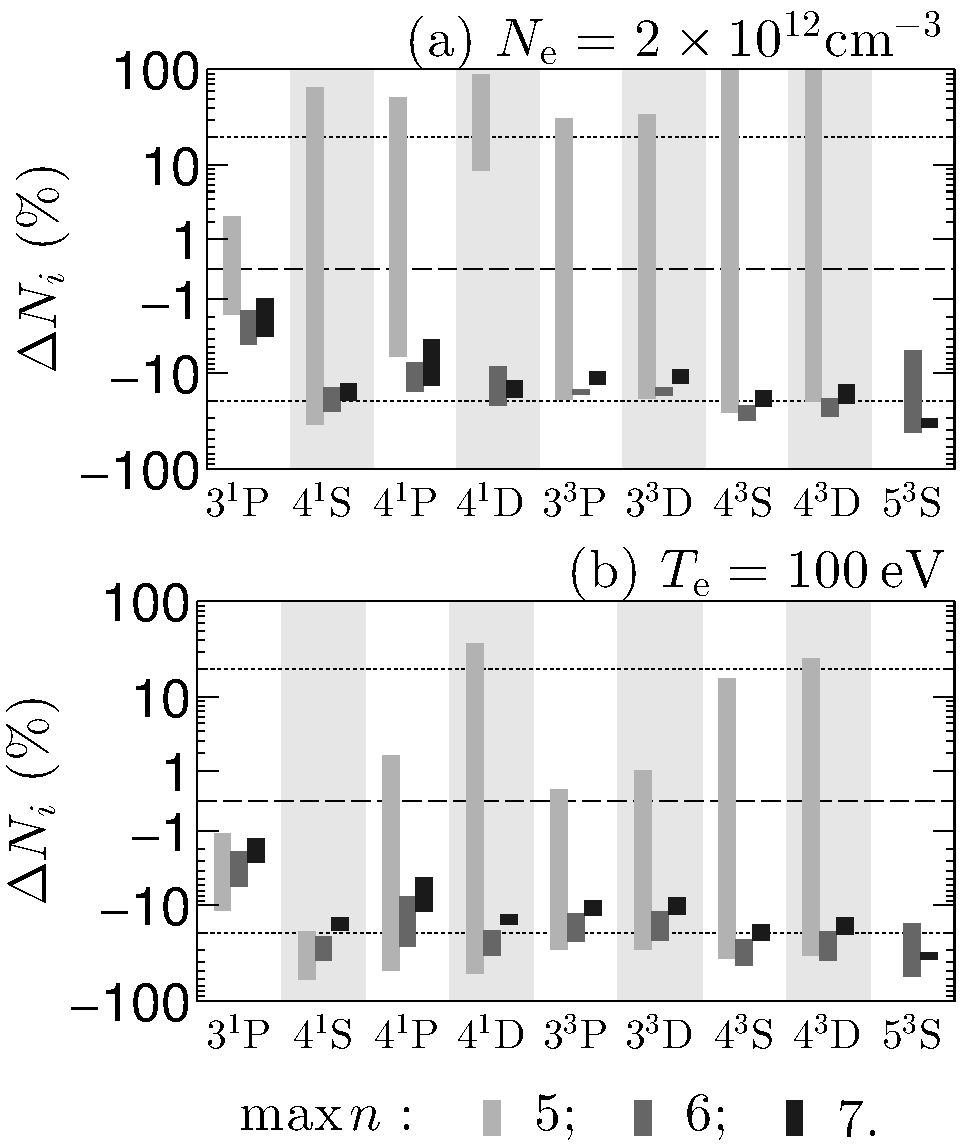
\includegraphics[width=0.7\textwidth]{levelabun-reldiff-maxn5to7-helines.pdf}
  \caption{包含至不同最高主量子数能级时,$n\leq4$ 能级的相对计算误差范围。图片来自 \onlinecite{xie:wlxb}。}
  \label{fig:chap03:levelabun-reldiff-all}
\end{figure}

以 $4^1{\rm S}$ 能级为例,图 \ref{fig:chap03:41S-levelabun-reldiff} 所示为该能级在碰撞辐射模型最高包含至不同 $\max n$ 时,计算结果的相对误差随电子温度或电子密度的变化。由图 \ref{fig:chap03:41S-levelabun-reldiff:1} 可见,随着 $T_{\rm e}$ 的升高,$\Delta N_{4^1{\rm S}}^{\max n=5}$ 自 $+40\%$ 急剧下降到 $-40\%$,虽然在 $T_{\rm e}\sim40\,{\rm eV}$ 附近,对于 $\max n=5$ 的碰撞辐射模型计算相对误差接近零,但总体来讲 $\max n=5$ 的碰撞辐射模型计算结果是不可接受的。$\Delta N_{4^1{\rm S}}^{\max n=5}$ 随 $N_{\rm e}$ 增长的变化规律类似(图 \ref{fig:chap03:41S-levelabun-reldiff:2}),当 $N_{\rm e}$ 自 $1\times10^{12}\,{\rm cm}^{-3}$ 至 $2\times10^{13}\,{\rm cm}^{-3}$ 变化时,$\Delta N_{4^1{\rm S}}^{\max n=5}$ 从 $+8\%$ 降低至 $-40\%$。当 $\max n$ 分别取 $6$ 和 $7$ 时,$\Delta N_{4^1{\rm S}}^{\max n=6}$ 和 $\Delta N_{4^1{\rm S}}^{\max n=7}$ 具有相同的变化趋势:随 $T_{\rm e}$ 的升高,计算误差短暂急剧上升之后,趋于平缓并有所下降(图 \ref{fig:chap03:41S-levelabun-reldiff:1});随着 $N_{\rm e}$ 的增长,计算误差增加(图 \ref{fig:chap03:41S-levelabun-reldiff:2})。$\Delta N_{4^1{\rm S}}^{\max n=6}$ 具有较大的误差数值,而 $\Delta N_{4^1{\rm S}}^{\max n=7}$ 在 $20\%$ 的相对误差范围内。

由图 \ref{fig:chap03:41S-levelabun-reldiff} 可以计算在特定的 $T_{\rm e}$ 或 $N_{\rm e}$ 参数下,各能级的计算误差 $\Delta_i^{\max n}$ 随另外一个参数变化时的总体范围,SUNIST 氦原子发射光谱实验(第 \ref{sec:chap04:sunist-spec-measurements} 节)所测量的氦原子谱线上能级计算结果如图 $\ref{fig:chap03:levelabun-reldiff-all}$ 所示。以此,我们可以得出在适用的等离子体参数范围内,碰撞辐射模型中最高包含至主量子数能级达什么程度时,其计算结果是可以接受的。当最高包含至 $\max n=5$ 时,计算结果的相对误差范围较大,甚至可达 $100\%$ 的范围,这是不可接受的;当最高包含至$\max n=6$ 时,计算误差范围开始缩小,但是对于用来进行谱线比诊断的 $n=4$ 能级粒子数的计算相对误差还是会超过 $20\%$;当 $\max n=7$ 时,除 $5^3{\rm S}$ 能级外的各能级粒子数计算结果的相对误差可以控制在 $20\%$ 以内。根据第 \ref{sec:chap04:uncertainty-transport} 节的分析,当 $n=4$ 能级与相邻能级之间电子碰撞跃迁速率系数存在不确定性时,其引起的能级粒子数密度相对计算误差即可达 $40\%$,由此,可以认为碰撞辐射模型中包含至最高主量子数为 $\max n=7$ 的能级时,计算结果已经可以接受,这与第 \ref{sec:chap03:level-selection} 节的处理相符。

图 \ref{fig:chap03:levelabun-reldiff-all} 还显示,当包含至更高能级时,粒子数的计算相对误差为负值。这是因为对 $n\ge 8$ 能级的舍弃切断了较低能级碰撞激发和电离的路径\cite{Fujimoto1979-HeCR},则碰撞辐射模型的计算中,包含至更高主量子数能级的能级数密度计算结果具有更低的值。%图 \ref{fig:chap03:levelabun-reldiff-all} 还显示
另外,在碰撞辐射模型取不同的 $\max n$ 时,各能级的数密度计算值具有强相关性。

\subsection{对谱线比计算结果影响的估计}

本文主要是利用碰撞辐射模型对氦原子谱线的相对强度进行等离子体 $T_{\rm e}$ 和 $N_{\rm e}$ 的诊断,通过下面的推导可以对碰撞辐射模型激发态数密度计算的不确定度对谱线强度比引起的影响进行估计。模型计算的来自 $q\to p$ 与 $j\to i$ 跃迁的两谱线强度比为:
\begin{equation}
\label{eq:chap03:lineratio-error}
r^{\rm mod}=\frac{A_{q\to p}n_q}{A_{j\to i}n_j},
\end{equation}
其中,爱因斯坦系数 $A_{q\to p}$ 与 $A_{j\to i}$ 的精度可以保证。则谱线比误差的主要来自模型对高能级数密度 $n_q$ 与 $n_j$ 的计算,可以写为\cite{burgos2012:PoP}:
\begin{equation}
\label{eq:chap03:ErrorModeledLineratio}
\begin{aligned}
\delta_r^{\rm mod} = & \pm r^{\rm mod}\\
& \times\sqrt{\left(\frac{\delta_{n_q}}{n_q}\right)^2 + \left(\frac{\delta_{n_j}}{n_j}\right)^2 - 2\gamma_{qj}\frac{\delta_{n_q}\delta_{n_j}}{n_qn_j}},
\end{aligned}
\end{equation}
其中,$\gamma_{qj}$ 代表 $q$ 与 $j$ 能级数密度的相关系数。假设$\delta_{n_q}/n_q\approx \delta_{n_j}/n_j=\delta_n/n$,则式 (\ref{eq:chap03:ErrorModeledLineratio}) 可以简化为:
\begin{equation}
\label{eq:chap03:SimpleErrorModeledLineratio}
r^{\rm mod} \approx\pm r^{\rm mod} \times \sqrt{2\left(\frac{\delta_n}{n}\right)^2(1-\gamma_{qj})},
\end{equation}
从式 (\ref{eq:chap03:SimpleErrorModeledLineratio}) 可以看出,对于激发态数密度具有高相关性的两条谱线,即 $\gamma_{qj}\sim 1$ 时,碰撞辐射模型计算的能级数密度误差可以抵消。

自旋单重态能级数密度之间与自旋三重态能级数密度之间具有高相关性,可以忽略单重态能级谱线之间与三重态能级谱线之间强度比的模型计算误差。单重态能级谱线强度与三重态能级谱线强度分别主要对 $T_{\rm e}$ 和 $N_{\rm e}$ 敏感,这可以解释图 \ref{fig:chap04:RelLevelabunAt3Times} 中显示的单重态与三重态能级数密度的碰撞辐射模型计算结果随 $T_{\rm e}$ 和 $N_{\rm e}$ 参数呈现出的集体变化趋势。由图 $\ref{fig:chap03:levelabun-reldiff-all}$ 可见,对于 $n=4$ 激发态各能级数密度的计算之间具有强的相关性,且相对计算误差小于 $20\%$,所以本文碰撞辐射模型的谱线比计算结果误差应远小于 $20\%$。

\section{SUNIST 等离子体谱线比诊断方法的建立}
\label{sec:chap03:lineratio-method}

\subsection{谱线强度比的选择}
\label{sec:chap03:lineratio-selection}

一般地,在氦原子发射光谱诊断实验中,人们选择来自 $n=3$ 激发态能级的三条谱线\pozhehao $667.8\,{\rm nm}\,(3^1{\rm D}-2^1{\rm P})$、$706.5\,{\rm nm}\,(3^3{\rm S}-2^3{\rm P})$ 和 $728.1\,{\rm nm}\,(3^1{\rm S}-2^1{\rm P})$ \pozhehao 的强度比进行 $T_{\rm e}$ 和 $N_{\rm e}$ 的诊断。但是,对于较高电子密度($N_{\rm e}>10^{13}\,{\rm cm}^{-3}$)的等离子体,$706.5\,{\rm nm}\,(3^3{\rm S}-2^3{\rm P})$ 谱线辐射在等离子体中会被强烈再吸收\cite{boivin2001,Boivin2007},此时氦等离子体实际的谱线测量结果与碰撞辐射模型也存在着明显的差别\cite{Schweer1992174,Brosda1993:Thesis,Sasaki:NIFS:DATA:346}。

SUNIST 等离子体对 $501.6\,{\rm nm}\,(3^1{\rm P}-2^1{\rm S})$、$396.5\,{\rm nm}\,(4^1{\rm P}-2^1{\rm S})$ 与 $388.9\,{\rm nm}\,(3^3{\rm P}-2^3{\rm S})$ 具有明显的再吸收作用(第 \ref{sec:chap04:lineratio-ne-te} 节),则这三条谱线也不适合用来进行谱线的辐射诊断,而谱线 $412.1\,{\rm nm}\,(5^3{\rm S}-2^3{\rm P})$ 来自 $n=5$ 壳层,其强度相对 $n=3$ 和 $n=4$ 壳层的谱线要弱。所以,本文在 $504.8\,{\rm nm}\,(4^1{\rm S}-2^1{\rm P})$、$492.2\,{\rm nm}\,(4^1{\rm D}-2^1{\rm P})$、$587.6\,{\rm nm}\,(3^3{\rm D}-2^3{\rm P})$、$471.3\,{\rm nm}\,(4^3{\rm S}-2^3{\rm P})$ 和 $447.1\,{\rm nm}\,(4^3{\rm D}-2^3{\rm P})$ 五条谱线中挑取分别来自不同自旋系统的三条谱线,建立同时进行 $T_{\rm e}$ 和 $N_{\rm e}$ 诊断的谱线比法。

\begin{figure}
  \centering
  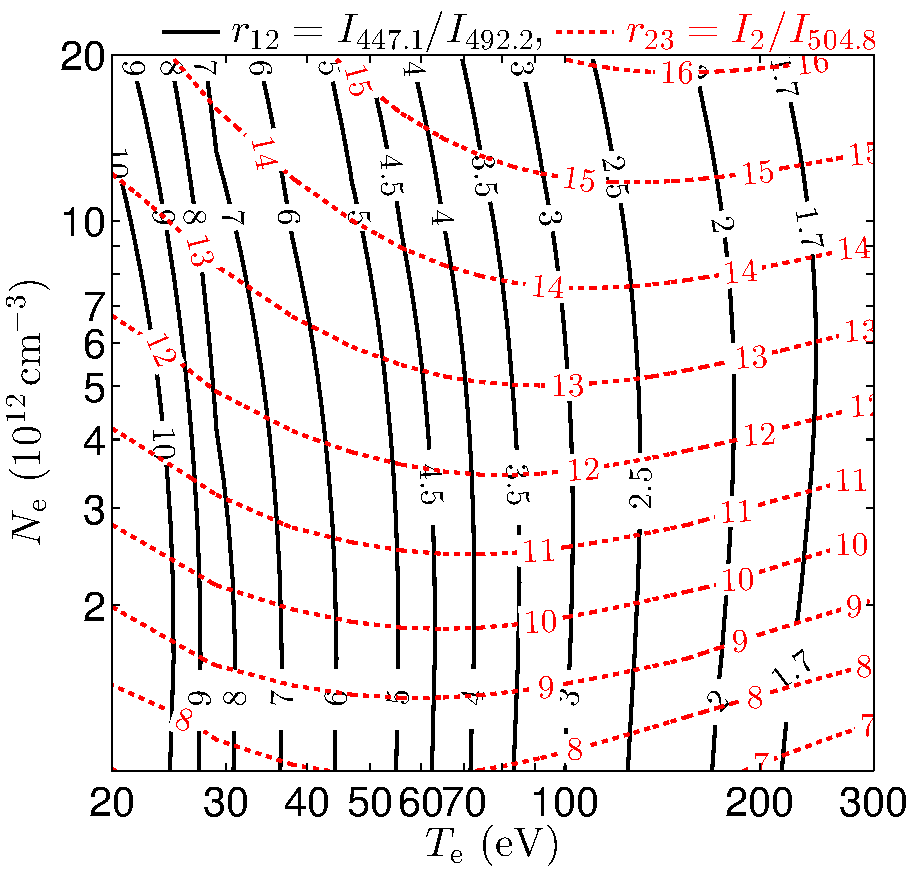
\includegraphics[width=0.6\textwidth]{1-9to7-7to5-getTeNe-lineratio.pdf}
  \caption{SUNIST 上使用的来自 $n=4$ 激发态能级的三条谱线的谱线比。图片来自 \onlinecite{xie:wlxb}。}
  \label{fig:chap03:getTeNe-lineratio}
\end{figure}

\begin{figure}
  \centering
  \begin{subfigure}{0.45\textwidth}
    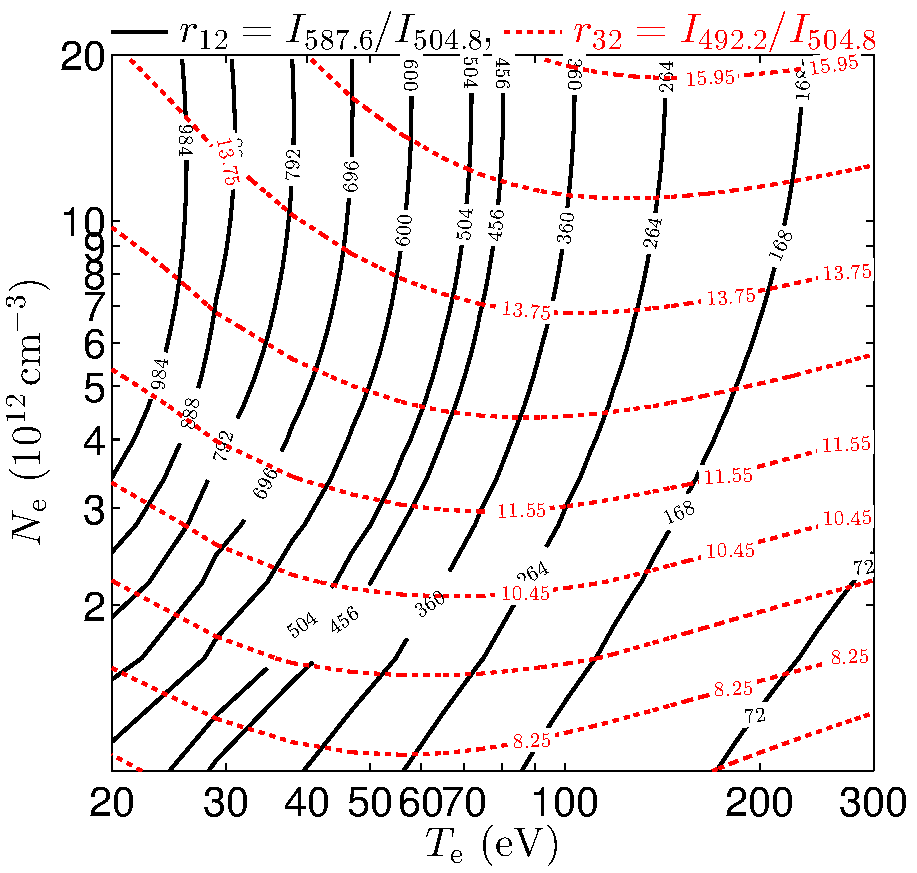
\includegraphics[width=\textwidth]{1-4to5-7to5-getTeNe-lineratio.pdf}
    \caption{}
    \label{fig:chap03:lineratio-backup:1}
  \end{subfigure}
  \hspace{0.05\textwidth}
  \begin{subfigure}{0.45\textwidth}
    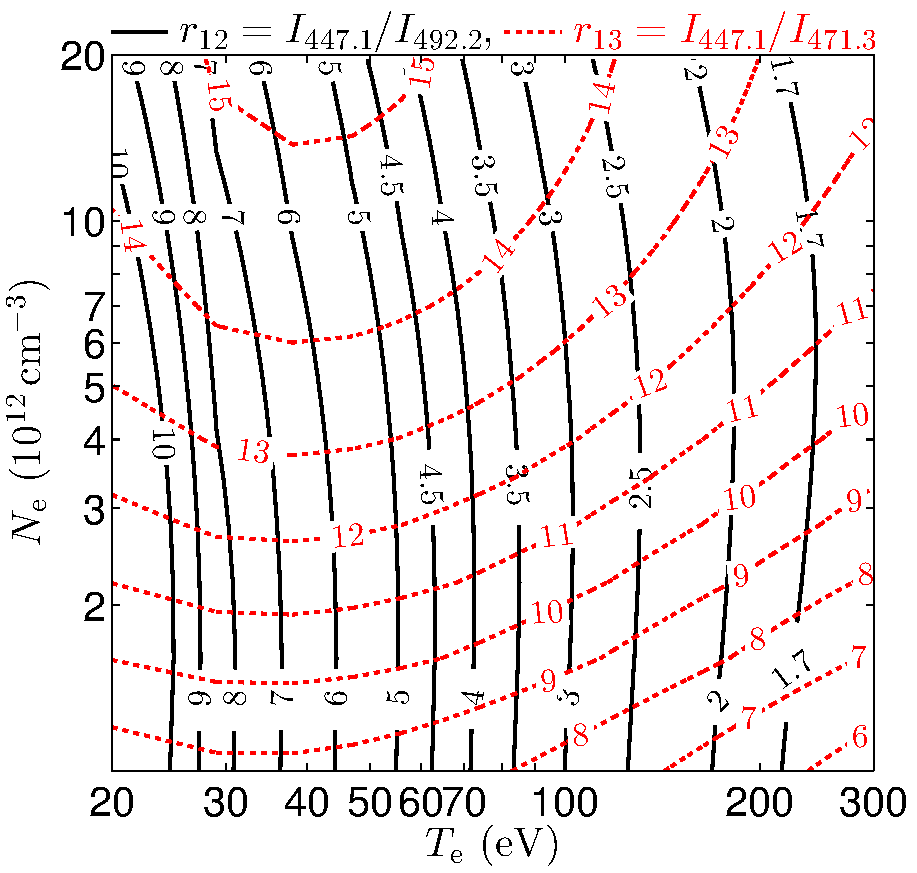
\includegraphics[width=\textwidth]{1-9to8-9to7-getTeNe-lineratio.pdf}
    \caption{}
    \label{fig:chap03:lineratio-backup:2}
  \end{subfigure}
  \caption{SUNIST 上可用来做谱线比诊断的其他谱线比备选方案}
  \label{fig:chap03:lineratio-backup}
\end{figure}

图 \ref{fig:chap03:getTeNe-lineratio} 与 图 \ref{fig:chap03:lineratio-backup} 分别显示本文所使用的谱线比计算结果与可以用来进行谱线比诊断的备选谱线比方案。其中,图 \ref{fig:chap03:lineratio-backup:1} 所显示的谱线比中,$T_{\rm e}$ 敏感谱线比 $r_{12}=I_{587.6}/I_{504.8}$ 在 $N_{\rm e}<5\times10^{12}\,{\rm cm}^{-3}$ 时,显示出与 $N_{\rm e}$ 较强的函数关系,同时此谱线比分别来自 $n=3$ 和 $n=4$ 的两激发态能级粒子,其强度差距悬殊,不利于谱线比法的应用。图 \ref{fig:chap03:lineratio-backup:2} 的备选方案中,$N_{\rm e}$ 敏感谱线比 $r_{13}=I_{447.1}/I_{471.3}$ 在低温高密度($T_{\rm e}<100\,{\rm eV}$,$N_{\rm e}>5\times10^{12}\,{\rm cm}^{-3}$)区,对电子温度的诊断会出现重复取值的问题。图 \ref{fig:chap03:getTeNe-lineratio} 显示的谱线比方案,谱线强度之间的比值范围合适,且电子温度和密度敏感的谱线比也显示出了优越的独立于另外一个参数的性质。

\subsection{谱线比法确定等离子体参数的过程}

\begin{figure}
  \centering
  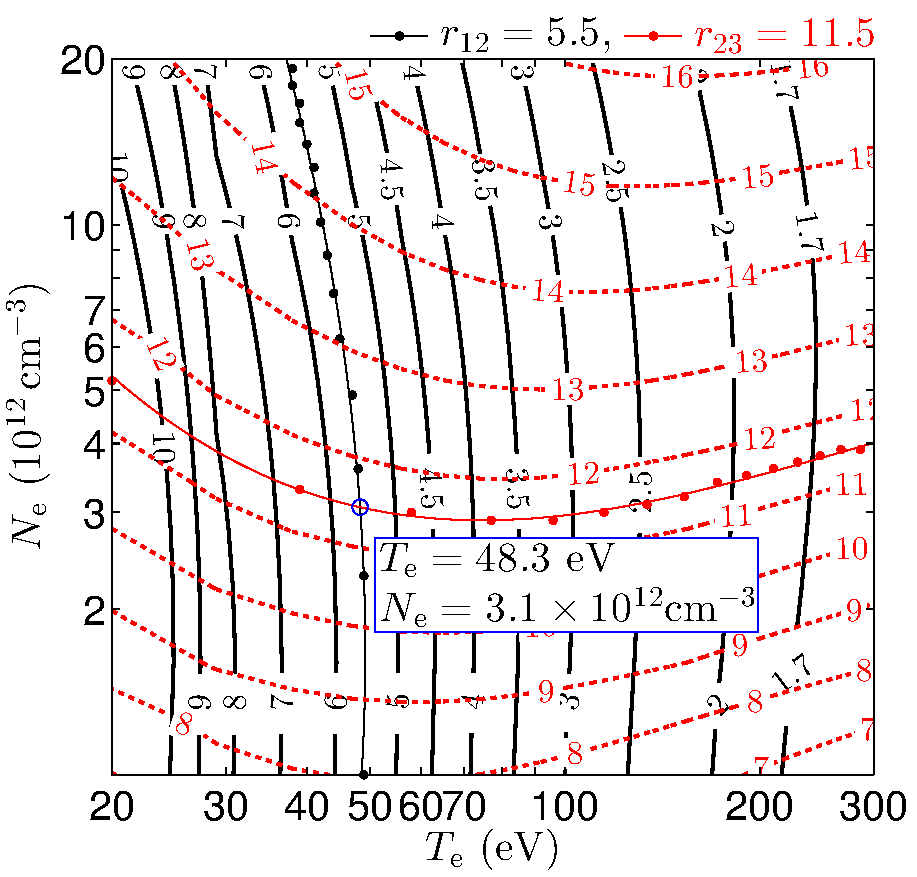
\includegraphics[width=0.6\textwidth]{5-9to7-7to5-getTeNe-crosspoint.pdf}
  \caption{谱线比法确定 $T_{\rm e}$ 和 $N_{\rm e}$ 参数}
  \label{fig:chap03:getTeNe-cross-pnt}
\end{figure}

以图 \ref{fig:chap03:getTeNe-lineratio} 中所示的谱线比计算结果为基础,图 \ref{fig:chap03:getTeNe-cross-pnt} 中以谱线比测量结果为 $r_{12}=5.5$,$r_{23}=11.5$ 时为例,显示了同时确定 $T_{\rm e}$ 和 $N_{\rm e}$ 的方法与过程。

1)寻点

在 $T_{\rm e}$、$N_{\rm e}$ 二维空间上的 $r_{12}(T_{\rm e},N_{\rm e})$ 与 $r_{23}(T_{\rm e},N_{\rm e})$ 计算值内,分别寻找 $r_{12}=5.5$ 和 $r_{23}=11.5$ 的 $(T_{\rm e}, N_{\rm e})$ 点,如图 \ref{fig:chap03:getTeNe-cross-pnt} 所示。

2)拟合

对于 $T_{\rm e}$ 敏感谱线比,将寻找到的一系列 $(T_{\rm e}, N_{\rm e})$ 寻点取值结果用下面的多项式进行拟合:
\begin{equation}
    \label{eq:chap03:getTeNe:r12-fit}
    T_{\rm e} = \sum_{i=0}^{3}C_{i}N_{\rm e}^{i}
\end{equation}
得到 $C_i$ 系数。

对于 $N_{\rm e}$ 敏感谱线比,则将 $(T_{\rm e}, N_{\rm e})$ 取值系里用下面的多项式拟合:
\begin{equation}
    \label{eq:chap03:getTeNe:r32-fit}
    N_{\rm e} = \sum_{j=0}^{3}C_{j}T_{\rm e}^{j}
\end{equation}
得到 $C_j$ 系数。多项式曲线拟合结果在图 \ref{fig:chap03:getTeNe-cross-pnt} 中给出。

3)求交点

联立方程 (\ref{eq:chap03:getTeNe:r12-fit}) 与 (\ref{eq:chap03:getTeNe:r32-fit}),求出其交点,则可以同时得到此交点的 $T_{e}$ 和 $N_{\rm e}$ 值,如图 \ref{fig:chap03:getTeNe-cross-pnt} 所示,当 $r_{12}=5.5$ 和 $r_{23}=11.5$ 时,等离子体的电子温度和电子密度参数分别为 $48.3\,{\rm eV}$ 和 $3.1\times10^{12}\,{\rm cm}^{-3}$。

\subsection{实际谱线比测量误差到 $T_{\rm e}$ 和 $N_{\rm e}$ 诊断误差传递的研究}
\label{sec:chap03:lineratio-error-to-result-error}

\begin{figure}%[H]
  \centering
  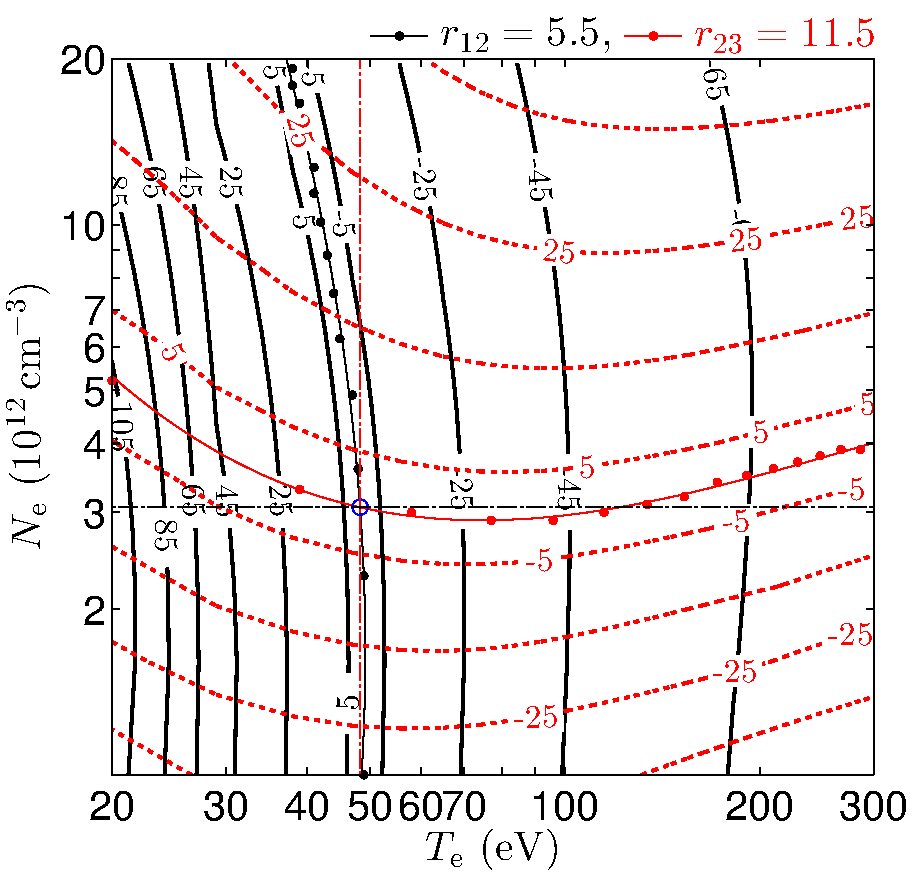
\includegraphics[width=0.6\textwidth]{6-9to7-7to5-getTeNe-errorroute.pdf}
  \caption{谱线比测量误差至 $T_{\rm e}$ 和 $N_{\rm e}$ 诊断误差传递的计算路径,其中谱线比等高线已经转换为了相对测量百分比误差等高线。}
  \label{fig:chap03:getTeNe-error-route}
\end{figure}

图 \ref{fig:chap03:getTeNe-cross-pnt} 中给出了谱线比法确定 $T_{\rm e}$ 和 $N_{\rm e}$ 的方法和过程,为了研究谱线比实验测量误差至 $T_{\rm e}$ 和 $N_{\rm e}$ 诊断结果误差的传递,在图 \ref{fig:chap03:getTeNe-error-route} 中,将谱线比等高线转换为相对图 \ref{fig:chap03:getTeNe-cross-pnt} 中示例谱线比的测量误差等高线。

对于电子温度 $T_{\rm e}$ 敏感谱线比 $r_{12}=I_{447.1}/I_{492.2}$,J.M.M. Burgos\cite{burgos2012:PoP} 计算了当电子密度 $N_{\rm e}$ 为固定值 $1.0\times10^{12}\,{\rm cm}^{-3}$ 时谱线比测量误差在不同 $T_{\rm e}$ 时对 $T_{\rm e}$ 诊断带来的误差,对应到图 \ref{fig:chap03:getTeNe-cross-pnt} 所示的谱线比法,则为 $N_{\rm e}=3.1\times10^{12}\,{\rm cm}^{-3}$ 时的计算路径,即图 \ref{fig:chap03:getTeNe-error-route} 中所示水平点画线。然而,仅通过 $T_{\rm e}$ 敏感谱线比是无法确定电子密度 $N_{\rm e}$ 参数的,在计算 $T_{\rm e}$ 敏感谱线比测量误差对 $T_{\rm e}$ 诊断结果影响时,固定 $N_{\rm e}$ 敏感谱线比值做为前提条件的计算路径是更符合实际情况的,即图 \ref{fig:chap03:getTeNe-error-route} 中所示 $r_{23}=11.5$ 的近似水平拟合实线曲线路径。

\begin{figure}%[H]
  \centering
    \begin{overpic}[width=0.6\textwidth]{7-9to7-7to5-getTeNe-errorpropagation.pdf}
    \put(0,0){\rotatebox{90}{\mbox{\colorbox{white}{\hspace{2em}谱线比误差 ($\%$)\hspace{2em}}}}}
    \put(-2,50){\rotatebox{90}{\mbox{\colorbox{white}{\hspace{2em}谱线比误差 ($\%$)\hspace{2em}}}}}
  \end{overpic}
  %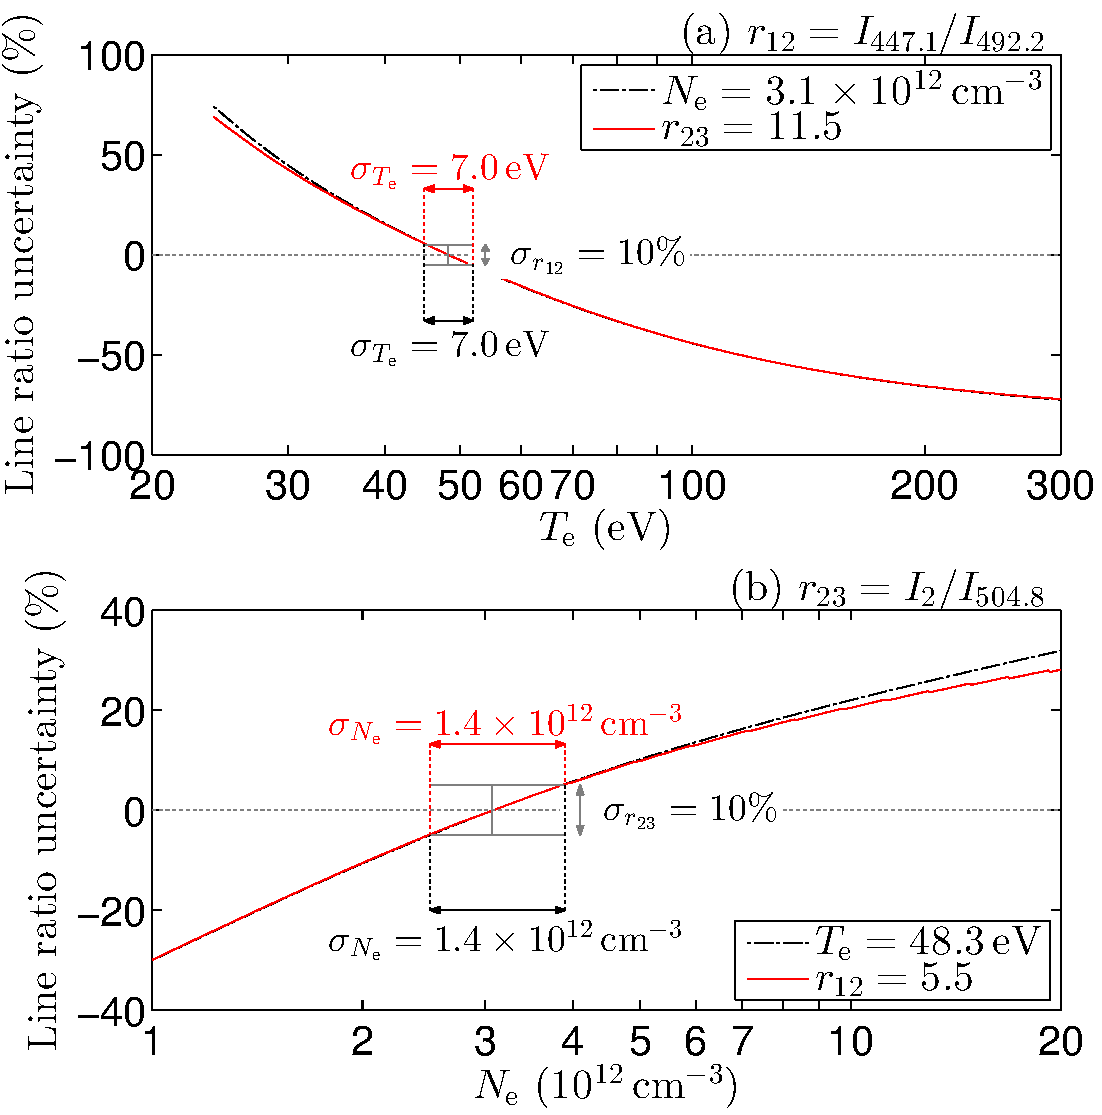
\includegraphics[width=0.6\textwidth]{7-9to7-7to5-getTeNe-errorpropagation.pdf}
  \caption{不同计算路径上的谱线比相对误差与等离子体参数诊断误差示意图。(a):$T_{\rm e}$ 敏感谱线比 $r_{12}$ 在固定 $N_{\rm e}$ 和固定 $r_{23}$ 时的计算路径;(b):$N_{\rm e}$ 敏感谱线比 $r_{23}$ 在固定 $T_{\rm e}$ 和固定 $r_{12}$ 时的计算路径。}
  \label{fig:chap03:getTeNe-errorpropagation}
\end{figure}

沿固定 $N_{\rm e}=3.1\times10^{12}\,{\rm cm}^{-3}$ 和固定 $r_{23}=11.5$ 计算路径的 $T_{\rm e}$ 敏感谱线比相对示例值 $5.5$ 的误差在图 \ref{fig:chap03:getTeNe-errorpropagation}(a) 中画出。由此可以计算出谱线比测量误差 $\sigma_{r_{12}}$ 所对应的 $T_{\rm e}$ 诊断误差值 $\sigma_{T_{\rm e}}$,如图 \ref{fig:chap03:getTeNe-errorpropagation}(a) 所示,当 $T_{\rm e}=48.3\,{\rm eV}$ 时,对于 $10\%$($\pm5\%$)的谱线比测量误差,两种不同路径计算的 $\sigma_{T_{\rm e}}$ 均为 $\sim7.0\,{\rm eV}$,因为两不同误差计算路径在此处具有相近的走向(图 \ref{fig:chap03:getTeNe-error-route})。由图 \ref{fig:chap03:getTeNe-errorpropagation}(a) 还可以得到,沿误差计算路径的谱线比误差曲线随 $T_{\rm e}$ 变化的斜率越大,谱线比测量误差引起的 $T_{\rm e}$ 诊断误差越小。

%在 $T_{\rm e}$ 为 $20-30\,{\rm eV}$ 时,两误差计算路径走向差别

\begin{figure}%[H]
  \centering
  \centering
    \begin{overpic}[width=0.6\textwidth]{8-9to7-7to5-getTeNe-errorpropagationscan.pdf}
    \put(0,18){\rotatebox{90}{\mbox{\colorbox{white}{ $\sigma_{T_{\rm e}}/T_{\rm e}$ ($\%$) }}}}
    \put(0,65){\rotatebox{90}{\mbox{\colorbox{white}{ $\sigma_{N_{\rm e}}/N_{\rm e}$ ($\%$) }}}}
  \end{overpic}
  %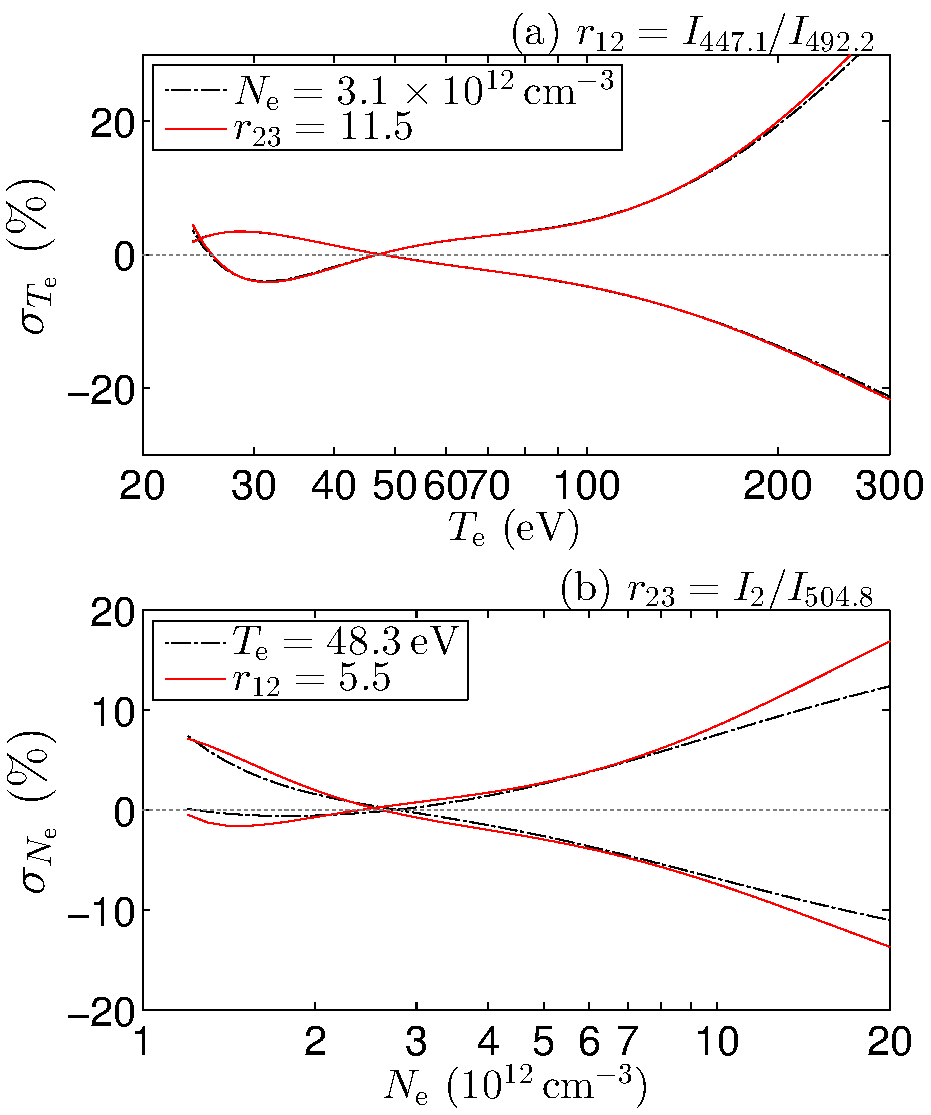
\includegraphics[width=0.6\textwidth]{8-9to7-7to5-getTeNe-errorpropagationscan.pdf}
  \caption{$10\%$ 的谱线比测量误差沿不同计算路径引起的相对诊断误差范围。(a):$\sigma_{T_{\rm e}}/T_{\rm e}$;(b):$\sigma_{N_{\rm e}}/N_{\rm e}$。}
  \label{fig:chap03:getTeNe-errorpropagationscan}
\end{figure}

以图 \ref{fig:chap03:getTeNe-errorpropagation}(a) 所示的计算方法,在不同的 $T_{\rm e}$ 情况下,$10\%$ 的 $r_{12}$ 测量误差沿不同误差计算路径对电子温度诊断的相对误差 $\sigma_{T_{\rm e}}/T_{\rm e}$ 范围曲线在图 \ref{fig:chap03:getTeNe-errorpropagationscan}(a) 中画出。可见,对于 $T_{\rm e}$ 敏感谱线比,当 $T_{\rm e}<100\,{\rm eV}$ 时,$\pm5\%$ 的谱线比测量结果误差所引起的 $T_{\rm e}$ 相对诊断误差范围在 $\pm10\%$ 以内。当 $T_{\rm e}>100\,{\rm eV}$ 时,谱线比法对电子温度的诊断开始对谱线比测量误差变得越来越敏感,对 $T_{\rm e}$ 诊断的相对误差范围会逐步增长至 $\pm20\%$ 以上。两不同误差计算路径之间具有微弱差别,这是因为在感兴趣的 $T_{\rm e}$ 范围内两路径的走向具有相近的走势,且与 $r_{12}$ 等高线的夹角也相近(图 \ref{fig:chap03:getTeNe-error-route})。

对于电子密度 $N_{\rm e}$ 敏感谱线比 $r_{23}=I_{492.2}/I_{504.8}$,固定 $T_{\rm e}=48.3\,{\rm eV}$ 与固定 $r_{12}=5.5$ 的谱线比测量误差至 $N_{\rm e}$ 诊断误差的计算路径分别由图 \ref{fig:chap03:getTeNe-error-route} 中竖直点画直线和近似竖直的 $r_{12}$ 实线拟合曲线表示。沿不同路径的 $r_{23}$ 谱线比相对误差和假设 $10\%$ 测量误差引起的 $\sigma_{N_{\rm e}}$ 在图 \ref{fig:chap03:getTeNe-errorpropagation}(b) 中画出,而在不同 $N_{\rm e}$ 时,谱线比测量误差对 $N_{\rm e}$ 诊断的相对误差范围曲线在图 \ref{fig:chap03:getTeNe-errorpropagationscan}(b) 中给出。可见,当 $N_{\rm e}>7.0\times10^{12}\,{\rm cm}^{-3}$ 时,谱线比法对电子密度的诊断开始对谱线比测量误差变得越来越敏感,对 $N_{\rm e}$ 诊断的相对误差范围由 $\pm10\%$ 以内增长到约 $\pm20\%$,而固定 $r_{12}$ 谱线比的路径比固定 $T_{\rm e}$ 的路径具有更大的诊断结果相对误差,因为在 $N_{\rm e}>7.0\times10^{12}\,{\rm cm}^{-3}$ 时,固定 $r_{23}$ 的计算路径与 $r_{23}$ 等高线的夹角比固定 $T_{\rm e}$ 路径更小,由图 \ref{fig:chap03:getTeNe-error-route} 可见,这是在较低 $T_{\rm e}$ 和较高 $N_{\rm e}$ 参数范围内,由 $N_{\rm e}$ 敏感谱线比 $r_{23}$ 的走向水平程度降低引起的,这样的结果也再次对第 \ref{sec:chap03:lineratio-selection} 节谱线比的选择进行了确认。

\section{小结}

用谱线比法获得等离子体 $T_{\rm e}$ 和 $N_{\rm e}$ 参数的诊断是以碰撞辐射模型在特定的电子温度和密度条件下对激发态数密度(即谱线强度)的预测为基础的。本章首先针对 SUNIST 等离子体条件建立了相应的氦原子碰撞辐射模型;结合对 SUNIST 上可利用的氦原子谱线的分析,选取了三条适合实际实验测量使用的谱线,并给出其谱线比的计算结果;最后给出了用谱线比法获取等离子体 $T_{\rm e}$ 和 $N_{\rm e}$ 参数的详细方法、过程以及谱线比实际测量中的误差对诊断结果所产生的影响。

其中,碰撞辐射模型对激发态数密度的计算精度为谱线比诊断的重点。本章基于各激发态能级主要产生过程的分析,推导出具有明确物理意义的速率系数不确定性传递函数,不仅可以对模型中使用的速率系数精度要求给出直接的依据,而且在模型的计算中可以对激发态数密度的计算结果进行直接估算。随着能级的升高,模型使用的反应过程速率系数精度也相应变差,导致模型中包含更多数目的能级和反应过程并不能如预期那样获得更高精度的结果。本章针对 SUNSIT 等离子体参数范围,通过比较分析,给出结论:当模型最高包含至 $\max n=7$ 壳层的激发态能级时,即给出可以接受的结果。


\graphicspath{{figures/chap04/}}

%\chapter{SUNIST 上光谱诊断系统和放电重复性的改善}
\chapter{SUNIST 上原子发射光谱的测量}
\label{chap:measureing-system}


本章首先介绍 SUNIST 上的诊断设备及光谱测量工作中的相关系统,然后对 SUNIST 发射光谱诊断测量系统的建立和标定以及基于重复放电的谱线测量方法进行描述,最后给出了 SUNIST 氦放电等离子体谱线测量与高斯拟合结果。其中,原子发射光谱测量系统在总装后对所使用单色仪进行了波长准确度、分辨率以及光谱响应进行了标定,通过屏蔽和隔离供电等措施对光电倍增管的谱线信号进行了噪声和基线干扰的抑制;SUNIST 实验中采用基于重复放电对氦等离子体的原子谱线进行测量,改善 SUNIST 放电的重复性不但可以获得具有重复宏观参数的等离子体放电,如气体原子激发、电离与复合等微观过程的重复性也得到了保证。

\section{SUNIST 上的诊断设备与相关系统}

\begin{figure}[H]
  \centering
  %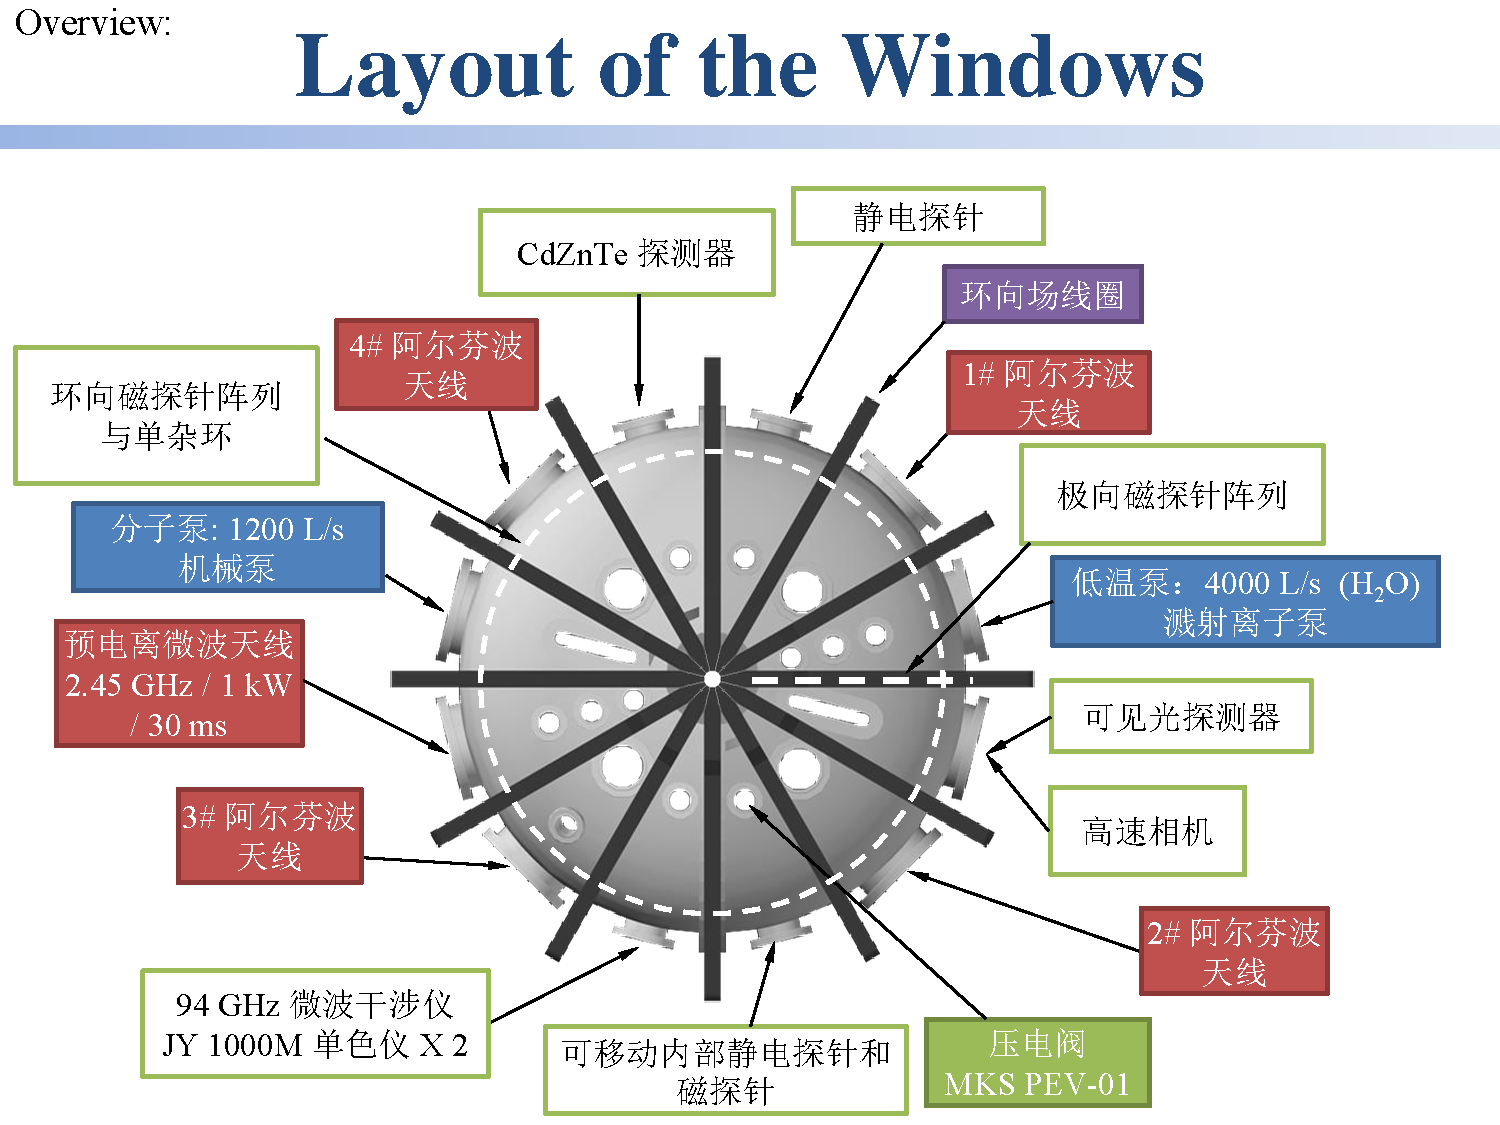
\includegraphics[width=\textwidth]{AvailableDiagnosticsOfSUNIST-1.jpg}
  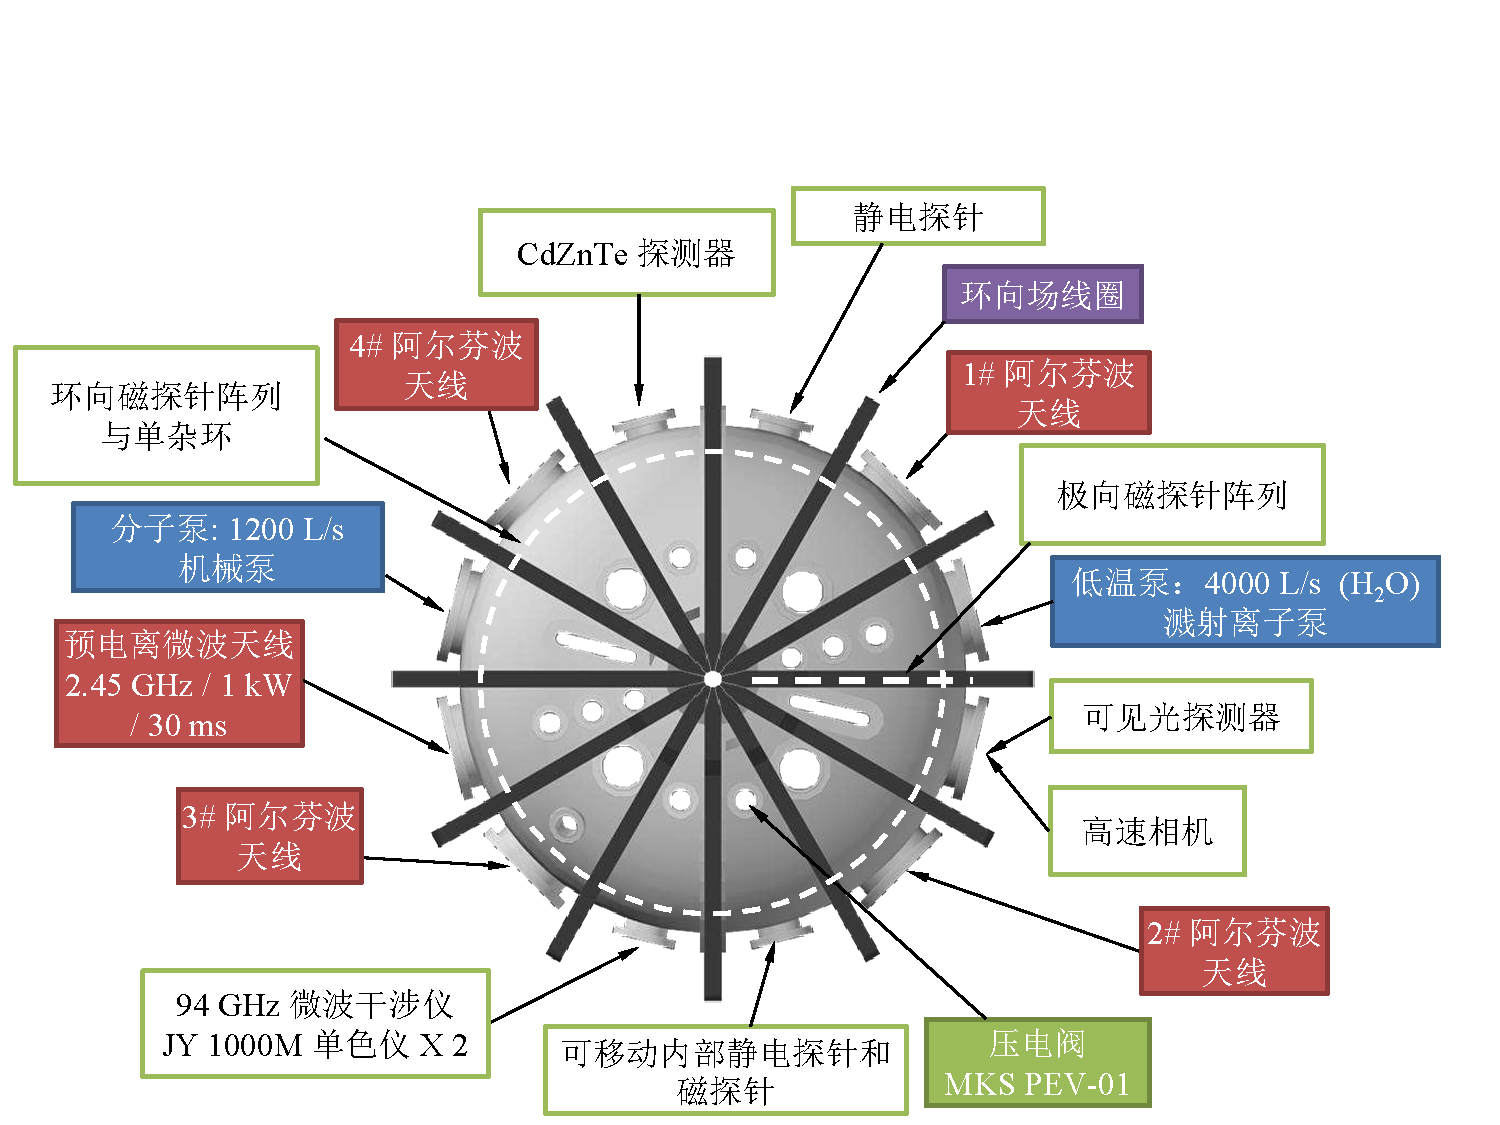
\includegraphics[width=\textwidth]{AvailableDiagnosticsOfSUNIST-14.pdf}
  \caption{SUNIST 上的诊断设备及相关系统(顶视图),修改自 \onlinecite{TanYi2013:1stA3}。}
  \label{fig:chap04:AvailableDiagnosticsOfSUNIST}
\end{figure}

SUNIST 上的诊断设备和相关系统布置情况如图 \ref{fig:chap04:AvailableDiagnosticsOfSUNIST} 所示。其中真空相关系统将在第 \ref{sec:chap04:gas-puffing-for-repeatability} 节中做详细介绍;本文在欧姆放电运行模式下进行光谱测量,而阿尔芬波与微波预电离天线为非感应等离子体启动和电流驱动研究时使用\cite{TanYi:HJBYDLZTWL:ECW,TanYi2008:Thesis,TanYi2011:NF:ECR},此处不再赘述。下面我们主要介绍 SUNIST 的诊断设备与它们在本文实验测量研究中所起的作用。

94 GHz 微波干涉仪与两台 JY 1000M-SII\cite{JY1000M} 单色仪安装在位于赤道面的小直径($d=100\,{\rm mm}$)窗口处,两台单色仪为本文原子光谱测量系统的主要设备(第 \ref{sec:chap04:spectroscopy-system} 节),微波干涉仪的诊断结果用来与本文谱线比法诊断结果进行对比(第 \ref{sec:chap04:lineratio-ne-te} 节);可移动内部静电探针和磁探针装置可以用来同时测量等离子体 $T_{\rm e}$、$N_{\rm e}$ 和磁场的径向分布,但其工作时需伸入等离子体内部,且探头尺寸较大,工作时会对等离子体造成较大影响,本文实验过程中不使用此装置;可见光探测器与高速相机安装于赤道面上的一个大尺寸($d=200\,{\rm mm}$)玻璃窗口上,可见光信号用来监测炮与炮之间放电的重复性(第 \ref{sec:chap04:repeat-shot-based-measure} 节),高速相机用来监视放电时的等离子体形态(第 \ref{sec:chap04:chord-integration} 节);极向和环向磁探针阵列用来测量等离子体的磁流体力学行为(第 \ref{sec:chap04:line-dbp10-fluctuation} 节);静电探针与单杂环信号分别可以提供边界等离子体的电子温度和密度参数与环电压信息,本文用其测量信号的标准差做为 SUNIST 等离子体放电重复性的指示(第 \ref{sec:chap04:gas-puffing-for-repeatability} 节);另外,CdZnTe 探测器测量等离子体的硬 X 射线辐射,可以为放电运行时等离子体状态判断提供参考。

\section{SUNIST 上原子发射光谱诊断系统}
\label{sec:chap04:spectroscopy-system}

\subsection{SUNIST上光谱测量系统与路径安排}

实验使用的发射光谱测量系统如图 \ref{fig:chap04:OESsystem} 所示。两条光纤通过石英玻璃窗口,在同一位置朝向相同方向收集 SUNIST 氦气放电等离子体发出的可见光,将收集到的可见光送至两台JY 1000M-SII 单色仪 Mono A 和 Mono B 的入口狭缝。经单色仪分光后,光线从单色仪的出口狭缝射出并被光电倍增管转换为光电流信号,该光电流信号经电流电压转换并被放大,最终被 SUNIST 装置上的数据采集系统进行模数转换并存入 MDSplus\cite{MDSplus:url,MDSplus:paper:1,MDSplus:paper:2} 数据库。
%电流信号,电流信号被转换为电压信号并放大,最终被数据采集器模数转换后存入 SUNIST 装置的 MDSplus\cite{MDSplus:url,MDSplus:paper:1,MDSplus:paper:2} 数据库系统。
单色仪光栅的旋转由用户通过计算机控制,数据采集系统的采样触发信号则由等离子体控制系统提供。

之所以在单色仪出口使用光电倍增管作为光探测器件,是为了保证测量的时间响应满足 SUNIST 脉冲放电等离子体(持续时间约 $10\,{\rm ms}$)的要求。虽然光电倍增管为单点探测器,但实验中两台单色仪配合使用,可以对两条谱线同时进行测量。

SUNIST 光谱测量路径如图 \ref{fig:chap04:measureing-route} 所示。在赤道面内,两条光纤通过石英玻璃窗口,在同一位置朝向真空室中心方向收集 SUNIST 氦气放电等离子体的辐射光。
%光纤接口的测量路径指向外凸的内真空室壁,这样在真空室内不安装多余部件以减少对真空本底影响的前提下,可以尽可能地减小真空室壁反射对测量的影响。
实验过程中,使用一台 94 GHz 微波干涉仪测量等离子体的平均电子密度 $\overline{N_{\rm e}}$。微波波束被聚焦后,从同一石英玻璃窗口沿图 \ref{fig:chap04:measureing-route} 中与光谱测量相同的路径打入真空室,在中心柱处被反射,被位于石英玻璃窗口前的喇叭天线接收。波束两次通过等离子体,由等离子体电子密度引起的相移需要计入两倍的沿测量路径的积分。

\begin{figure}[H]
  \centering
  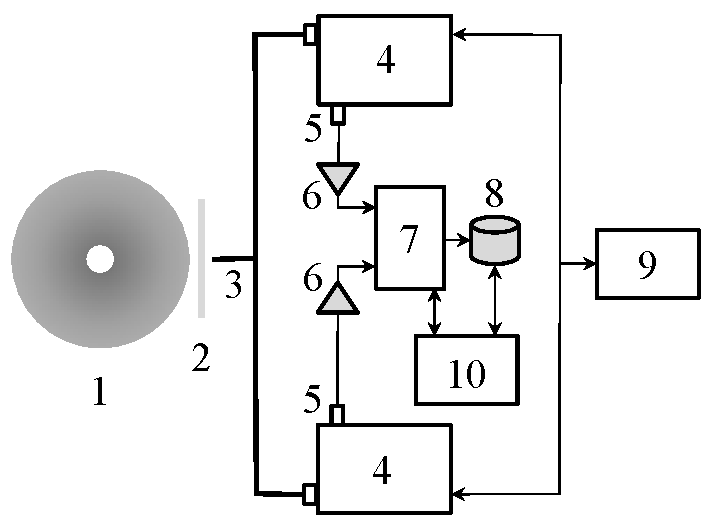
\includegraphics[width=0.6\textwidth]{OESsystem.pdf}
  \caption{SUNIST 实验光谱测量设备示意图。\quad 1:氦气放电等离子体赤道面;2:石英窗口;3:光纤;4:单色仪;5:光电倍增管;6:信号放大器;7:数据采集器;8:数据库服务器;9:控制计算机;10:托卡马克与等离子体控制系统。粗实线表示光纤连接,细实线表示电信号或数据连接。图片来自 \onlinecite{xie:istw2011}。}
  \label{fig:chap04:OESsystem}
\end{figure}

\begin{figure}[H]
  \centering
  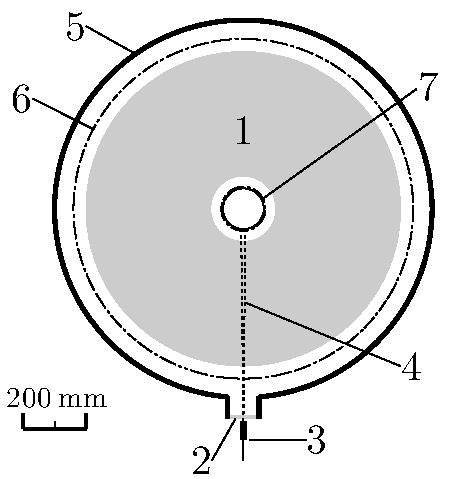
\includegraphics[width=0.5\textwidth]{instru-alignments-2.pdf}
  \caption{SUNIST 光谱测量路径图。\quad 1:SUNIST 氦气放电等离子体赤道面;2:石英玻璃窗口;3:光纤接口与准直孔;4:单色仪与 $94\,{\rm GHz}$ 微波干涉仪的测量路径;5:外真空室壁;6:外限制器边缘;7:内真空室壁与内限制器边缘。图片来自 \onlinecite{xie:wlxb}。}
  \label{fig:chap04:measureing-route}
\end{figure}


\subsection{SUNIST 上使用的单色仪参数与标定}

%\begin{table}
%\caption{JY 1000M-SII~单色仪测量汞灯谱线时不同的狭缝宽度组合}
%\label{table:chap04:different-slit-width}
%\begin{center}
%\begin{tabular}{cccccc}
%\toprule[1.5pt]
%     \multirow{2}{*}{序号} & \multicolumn{2}{c}{A~单色仪} & & \multicolumn{2}{c}{B~ 单色仪}
%     \cr\cline{2-3}\cline{5-6}
%     & 入口狭缝 ($\mu$m) & 出口狭缝 ($\mu$m) & & 入口狭缝 ($\mu$m) & 出口狭缝 ($\mu$m)\\
%\midrule[1pt]
%     1 & 10 & 10 & & 10 & 10\\
%     2 & 25 & 25 & & 25 & 10\\
%     3 & 50 & 10 & & 50 & 10\\
%     4 & 75 & 6  & & 75 & 10\\
%     5 & 100 & 6 & & 100 & 10\\
%     6 & 150 & 6 & & 150 & 10\\
%     7 & 200 & 6 & & 200 & 10\\
%\bottomrule[1.5pt]
%\end{tabular}
%\end{center}
%\end{table}

%\begin{figure}
%    \centering
%    \begin{subfigure}{0.47\columnwidth}
%        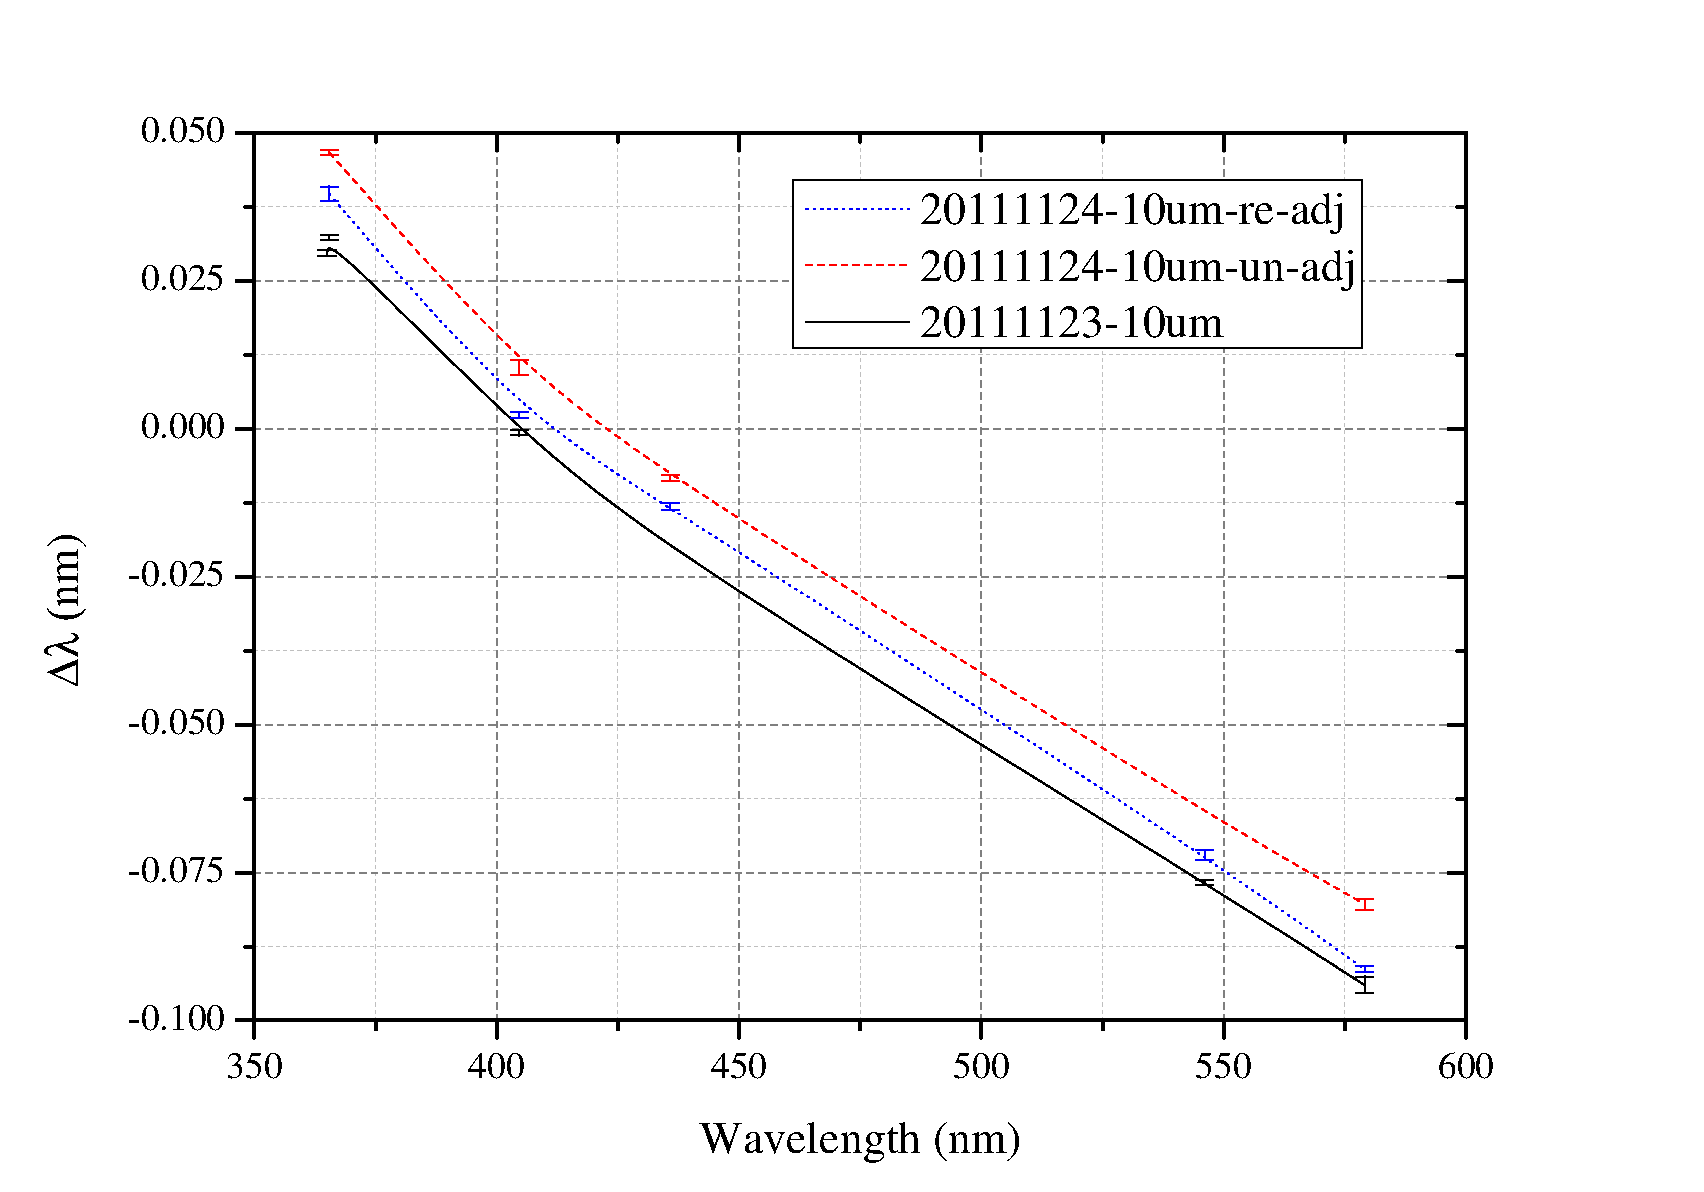
\includegraphics[width=\columnwidth]{A-delta-lambda-pre-un-re-adj-10um.pdf}
%        \caption{重新校准前后的波长准确度}%
%        \label{fig:chap03:linearity}
%    \end{subfigure}
%    %\hspace{0.05\textwidth}
%    \begin{subfigure}{0.47\columnwidth}
%        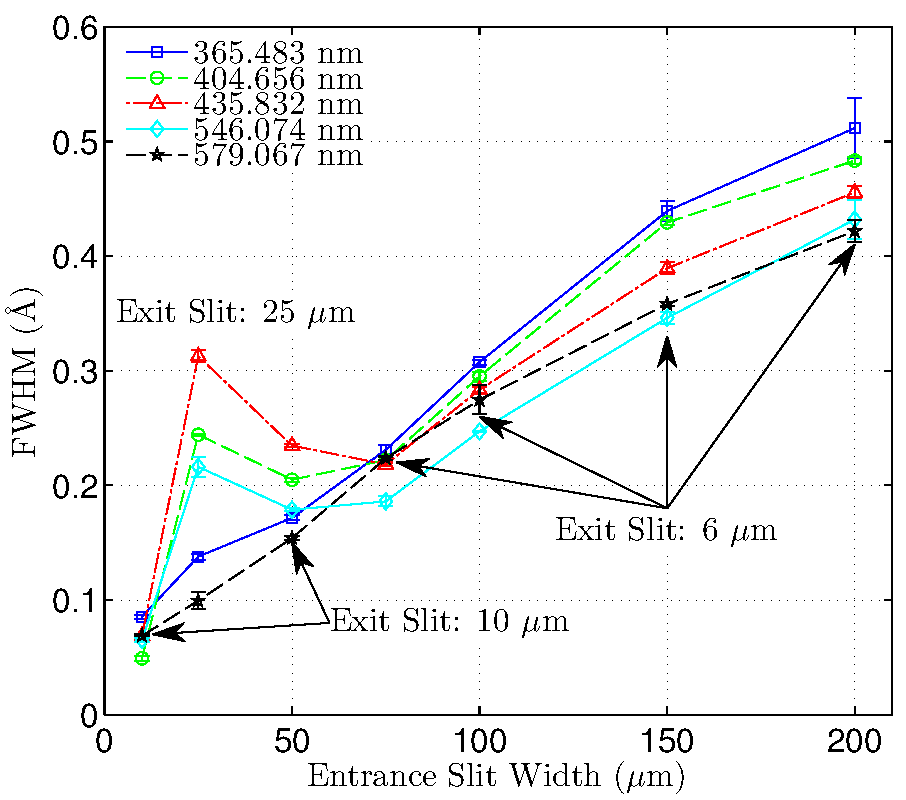
\includegraphics[width=\columnwidth]{A-FWHM-vs-slit-width.pdf}
%        \caption{不同狭缝宽度的分辨率}%
%        \label{fig:chap03:resolution}
%    \end{subfigure}
%    \caption{A 单色仪的波长准确度与谱线分辨率}%
%    \label{fig:chap03:A-linearity-and-resolution}
%\end{figure}
%
%\begin{figure}
%    \centering
%    \begin{subfigure}{0.47\columnwidth}
%        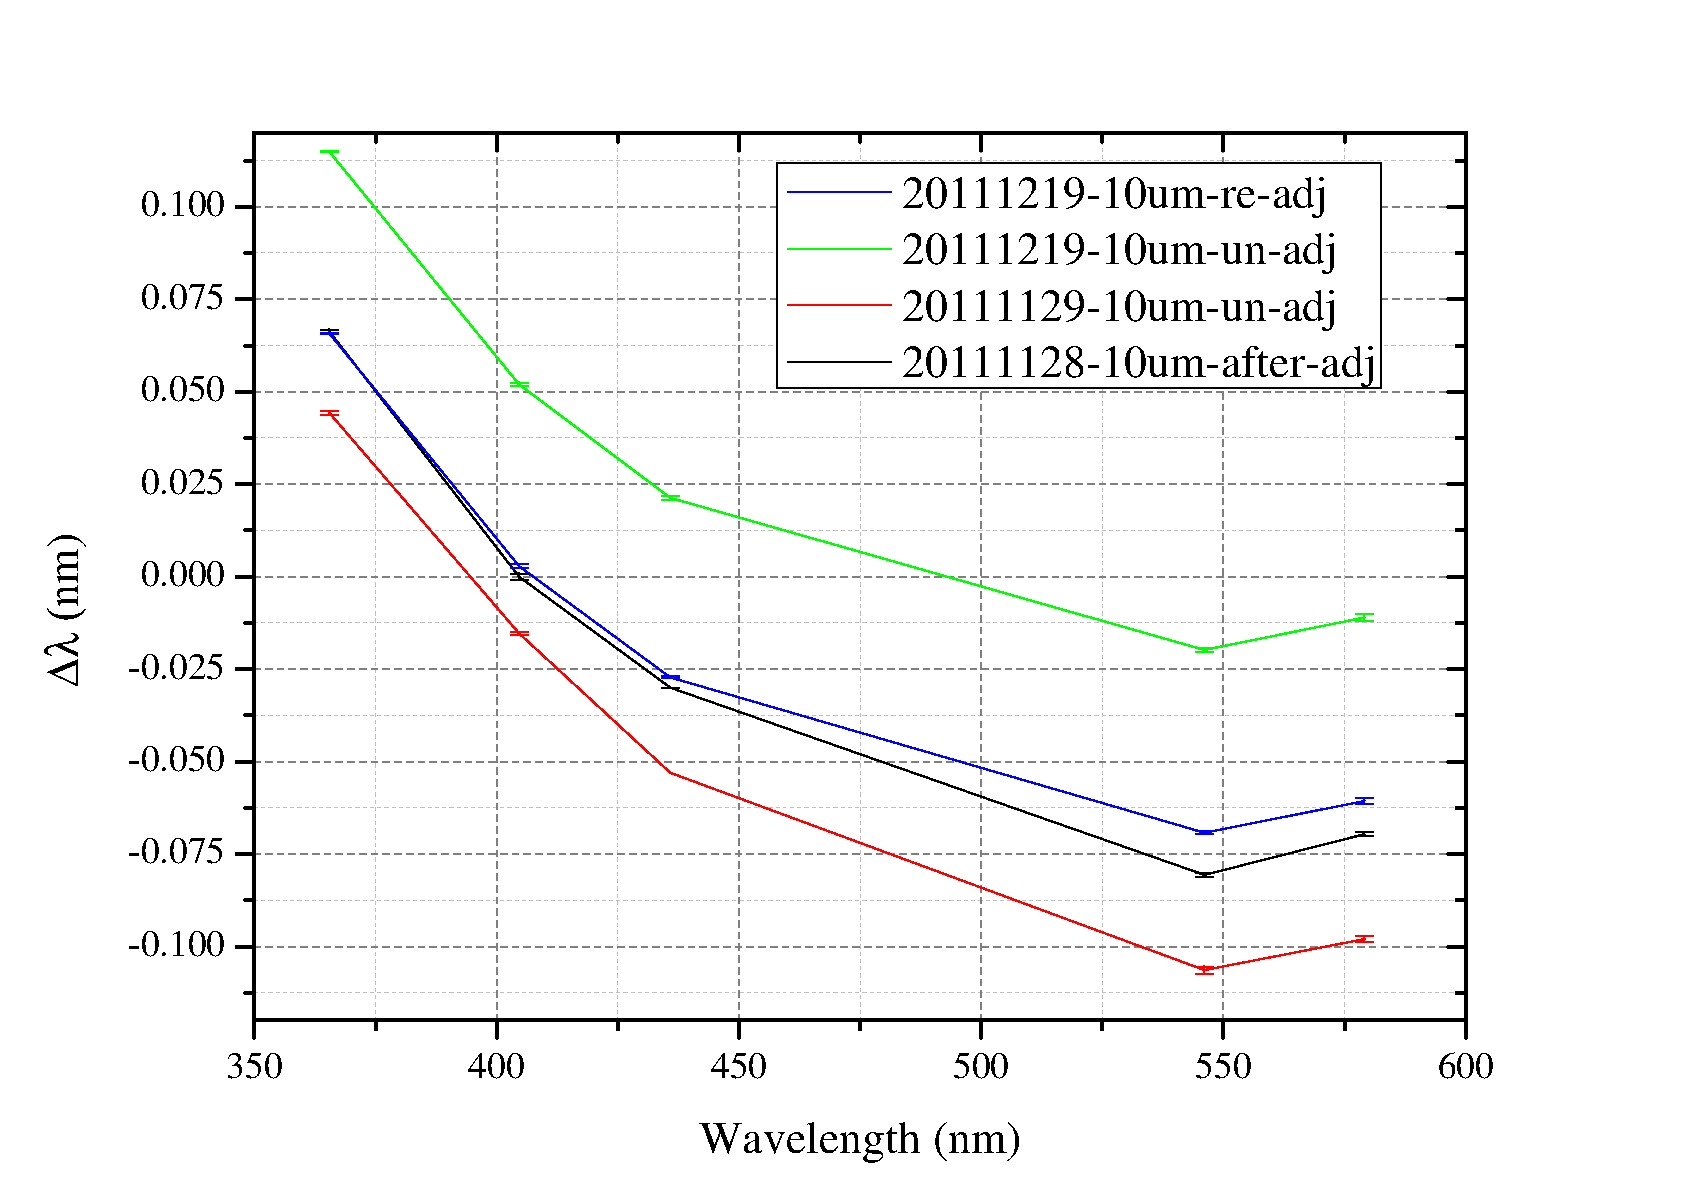
\includegraphics[width=\columnwidth]{B-delta-lambda-10um-111219.pdf}
%        \caption{重新校准前后的波长准确度}%
%        \label{fig:chap03:41S-levelabun-reldiff:1}
%    \end{subfigure}
%    %\hspace{0.05\textwidth}
%    \begin{subfigure}{0.47\columnwidth}
%        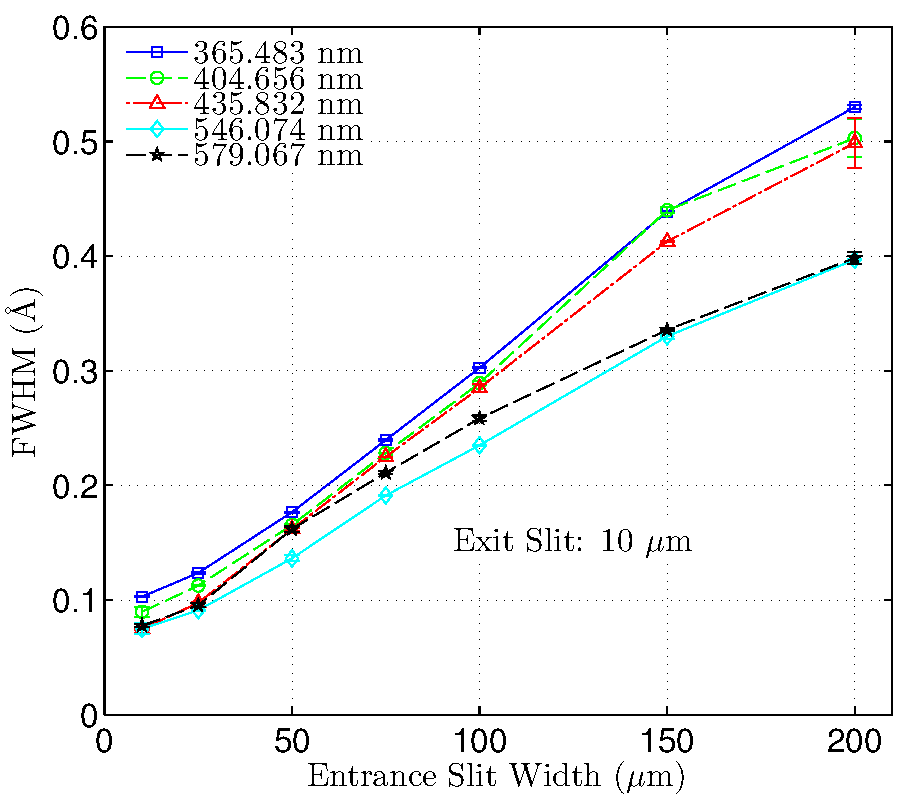
\includegraphics[width=\columnwidth]{B-FWHM-vs-slit-width.pdf}
%        \caption{不同狭缝宽度的分辨率}%
%        \label{fig:chap03:11S-levelabun-reldiff:2}
%    \end{subfigure}
%    \caption{B 单色仪的波长准确度与谱线分辨率}%
%    \label{fig:chap03:41S-levelabun-reldiff}
%\end{figure}

实验使用两台 JY 1000M-SII 单色仪进行氦放电等离子体的发射光谱测量,其基本参数如表 \ref{table:chap04:1000m_spec} 所示。实际测量中,需要根据要测量的谱线的强度调整入口和出口狭缝宽度,以达到合适的信号幅度,并在重复放电的基础上,对谱线进行扫描。实验前,使用汞灯对单色仪的波长准确度和波长分辨率进行了标定,并使用钨灯对单色仪的光谱相对响应进行标定,本节给出单色仪的各项指标标定结果。

\begin{table}[H]
\caption{JY 1000M-SII~单色仪的参数}
\label{table:chap04:1000m_spec}
\begin{center}
\begin{tabular}{ccc}
\toprule[1.5pt]
     焦距 $F_{\rm mono}$ (mm) & 色散 $D_{\rm mono}$ (nm/mm) & 分辨率 $R_{\rm mono}$ (nm) \\
%\midrule[1pt]
     $1000$ & $0.4$ & $0.004$ \\
\midrule[1pt]
      波长范围 (nm) & 光栅与中心波长 $\lambda_{\rm c, mono}$ & 入、出口狭缝 $W_{\rm ent}$、$W_{\rm ex}$ ($\mu$m) \\
%\midrule[1pt]
     $250-750$ & $2400\,{\rm g}/{\rm mm}$ @ $400\,{\rm nm}$ & $0-2000$ \\
\bottomrule[1.5pt]
\end{tabular}
\end{center}
\end{table}

\subsubsection{标定中使用的汞灯谱线}

图 \ref{fig:chap04:shape-of-Hg-lines} 所示为单色仪标定过程中使用的汞灯谱线\cite{Hg-lamp-lines}线形,其中:

\begin{figure}[H]
	\centering
    \begin{overpic}[width=0.5\textwidth]{A-shape-of-Hg-lines.pdf}
        \put(25,1){\mbox{\colorbox{white}{\hspace{1.1em} 波长差 ($\rm nm$)\quad}}}
        \put(0,42){\rotatebox{90}{\mbox{\colorbox{white}{\hspace{2em}$I$ ($\rm a.u.$)\hspace{4em}}}}}
    \end{overpic}
	%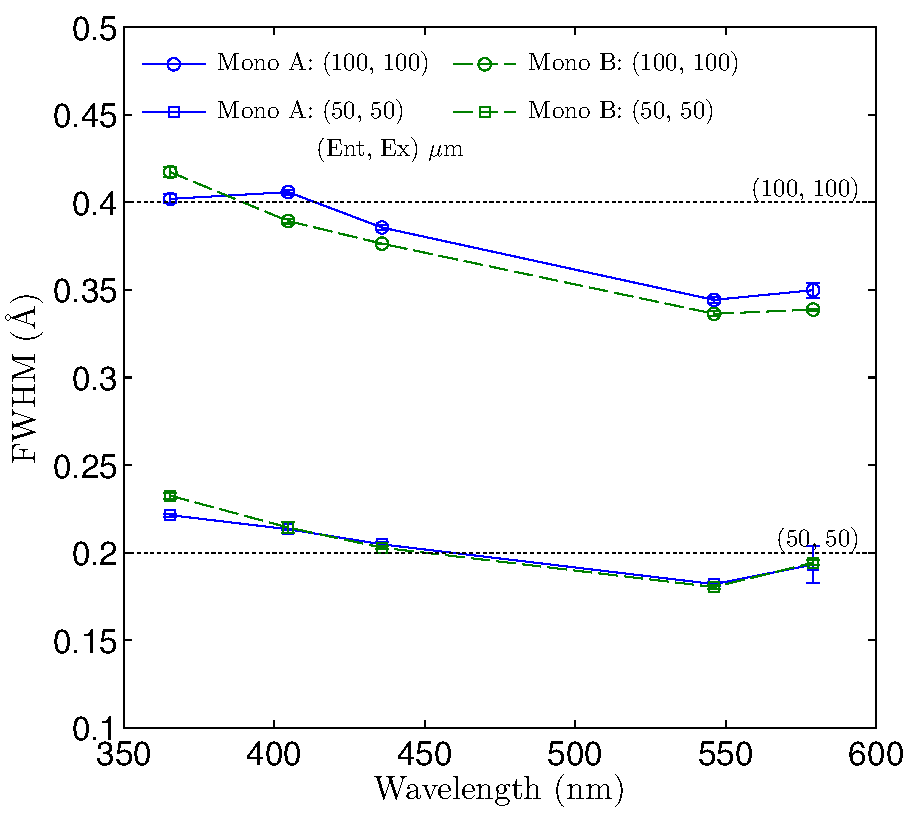
\includegraphics[width=0.6\textwidth]{A-B-FWHM-vs-wavelength-and-diff-slits-width.pdf}
    \caption{标定中汞灯的谱线线形}
	\label{fig:chap04:shape-of-Hg-lines}
\end{figure}

\begin{itemize}
	\item 汞灯窗口使用了普通光学玻璃,导致 $253.652\,{\rm nm}$ 与 $313.155\,{\rm nm}$ 的汞线强度弱。
	\item 汞的激发态能级具有精细结构,每条线均存在谱线分裂叠加的不规则形状,这对单色仪进行仪器线形(instrumental profile)或谱线分辨率的标定不利。
	\item 实际托卡马克光谱测量中使用了较宽的入口和出口狭缝,此时的仪器线形展宽远大于汞灯谱线宽度,汞灯谱线精细结构的影响可以忽略。实际操作中,将测量到的汞灯谱线宽度作为仪器展宽。
	\item $365.016\,{\rm nm}$ 与 $365.483\,{\rm nm}$ 谱线波长接近,标定过程中只取 $365.483\,{\rm nm}$ 线。
	\item $365.016\,{\rm nm}$ 与 $546.074\,{\rm nm}$ 线线形较干净,当入口和出口狭缝宽度较窄时可以用来标定仪器线形。
\end{itemize}

\subsubsection{单色仪波长准确度和分辨率标定结果}

\begin{figure}%[H]
    \centering
    \begin{subfigure}{0.8\columnwidth}
        \begin{overpic}[width=\columnwidth]{A-delta-lambda-pre-un-re-adj-10um.pdf}
            \put(35,0.5){\mbox{\colorbox{white}{\hspace{2.5em} 波长 ($\rm nm$)\hspace{2.5em}}}}
        \end{overpic}
        %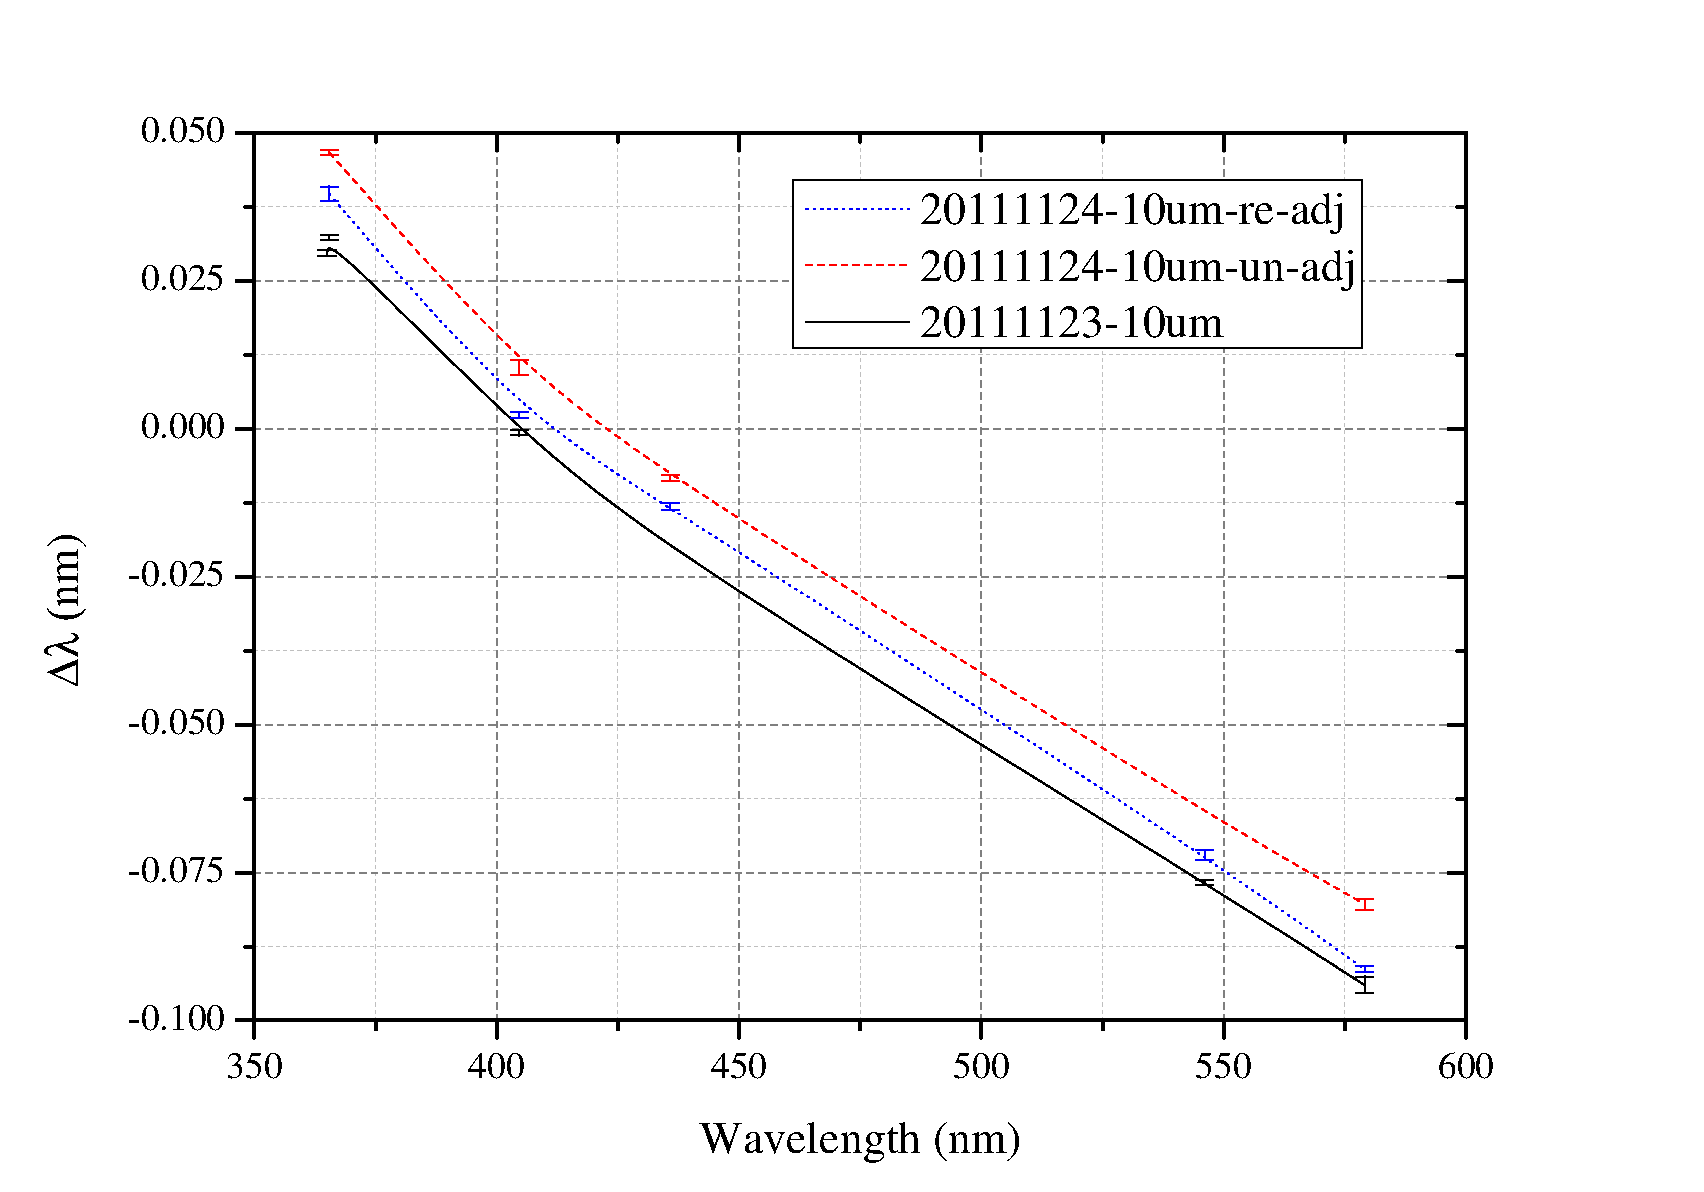
\includegraphics[width=\columnwidth]{A-delta-lambda-pre-un-re-adj-10um.pdf}
        \caption{A 单色仪波长准确度}%
        \label{fig:chap03:delta-lambda-a}
    \end{subfigure}
    \\[2em]
    %\hspace{0.03\textwidth}
    \begin{subfigure}{0.8\columnwidth}
        \begin{overpic}[width=\columnwidth]{B-delta-lambda-10um-111219.pdf}
            \put(35,0.5){\mbox{\colorbox{white}{\hspace{2.5em} 波长 ($\rm nm$)\hspace{2.5em}}}}
        \end{overpic}
        %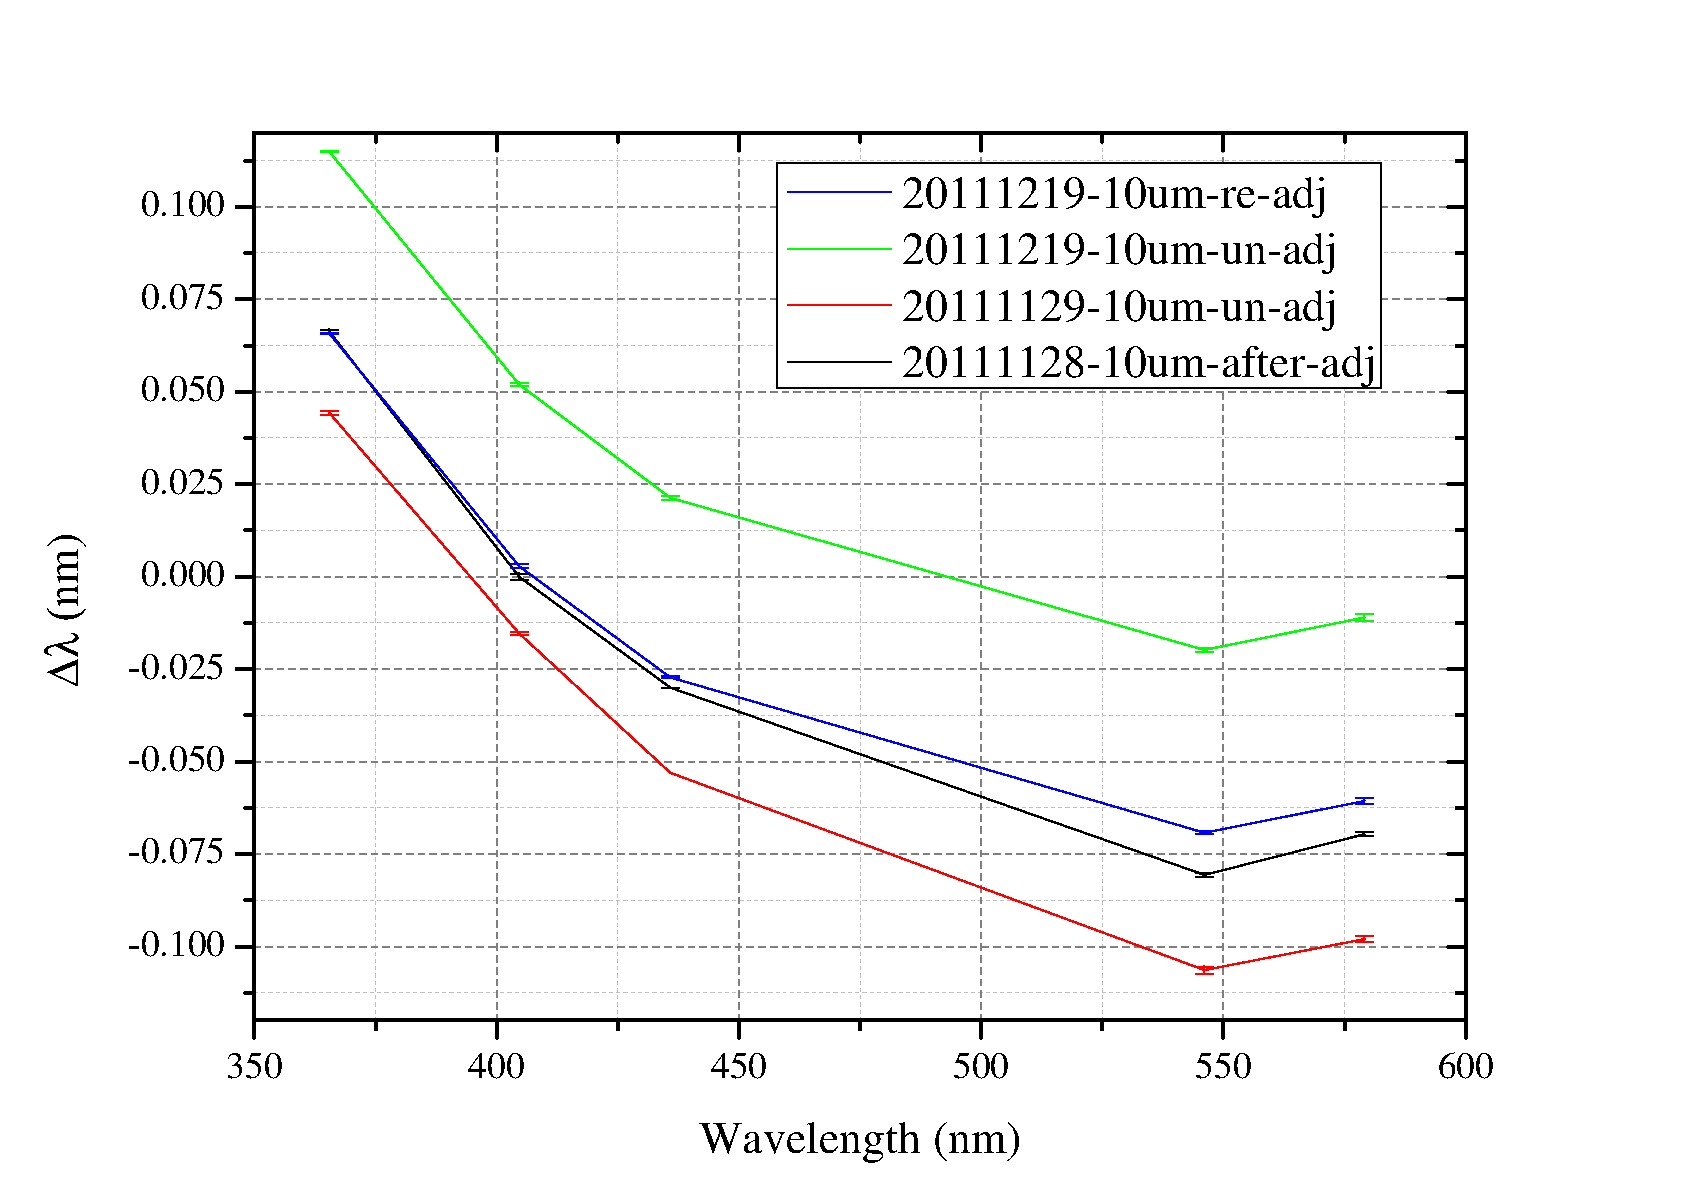
\includegraphics[width=\columnwidth]{B-delta-lambda-10um-111219.pdf}
        \caption{B 单色仪波长准确度}%
        \label{fig:chap03:delta-lambda-b}
    \end{subfigure}
    \caption{A 单色仪与 B 单色仪校准前后的波长准确度}%
    \label{fig:chap03:delta-lambda}
\end{figure}

\begin{figure}%[H]
	\centering
    \begin{overpic}[width=0.7\textwidth]{A-B-FWHM-vs-wavelength-and-diff-slits-width.pdf}
        \put(40,0.5){\mbox{\colorbox{white}{\hspace{1.1em} 波长 ($\rm nm$)\hspace{2.5em}}}}
    \end{overpic}
	%\includegraphics[width=0.6\textwidth]{A-B-FWHM-vs-wavelength-and-diff-slits-width.pdf}
    \caption{A 单色仪与 B 单色仪在实验测量条件下测得的分辨率,两条水平虚线所示为只考虑狭缝宽度时的单色仪分辨率。括号里面的数值 $({\rm Ent}, {\rm Ex})$ 分别为入口狭缝和出口狭缝的宽度,单位为 $\mu{\rm m}$。}
	\label{fig:chap04:resolution:experiment-layout}
\end{figure}

单色仪使用光栅的闪耀波长为 $400\,{\rm nm}$,汞灯 $404.656\,{\rm nm}$ 线恰好适合用来进行单色仪的波长校准。厂家给出的波长准确度数据为 $\pm0.05\,{\rm nm}$,图 \ref{fig:chap03:delta-lambda} 所示为可见光波段两单色仪在不同波长位置的波长准确度标定结果,
%, 以及单色仪在波长标定前后和波长准确度的稳定性的测量结果.
标定过程中发现,单色仪的入口和出口狭缝宽度宽度对波长准确度的影响可以忽略。

图 \ref{fig:chap03:delta-lambda-a} 所示为 A 单色仪波长准确度在波长重新校准前后以及波长准确度在前后连续两天的稳定性测量结果。可以看出单色仪的波长准确度比厂家给出的指标略差,但处于可接受的范围内。A 单色仪的波长准确度随波长的增加线性递减,波长重新校准前后,波长误差曲线只是简单平移,说明 A 单色仪在其测量范围内的波长准确度线性较好,其波长误差范围为 $+0.05\,{\rm nm}\sim -0.10\,{\rm nm}$。随着环境温度或湿度的影响,单色仪光路会发生微弱的相对位移,这会影响单色仪的波长准确度,经过长时间的观察测量,A 单色仪波长准确度的稳定性为 $\pm0.08\,{\rm nm}$。

图 \ref{fig:chap03:delta-lambda-b} 所示为 B 单色仪波长准确度在重新校准前后以及波长准确度在相隔较长时间(约 20 天)时稳定性的测量结果。可以看出 B 单色仪的波长准确度范围为 $\pm0.10\,{\rm nm}$,比 A 单色仪稍差,且 B 波长线性也不够好,中心波长重新校准前后,波长误差校准量在不同汞线波长处不尽相同,波长越长,波长校准量越大一些。经过一段时间的观察测量,其波长准确度的稳定性为 $\pm0.12\,{\rm nm}$。

在实验中,两台单色仪的入口和出口狭缝宽度设为 $50\,\mu{\rm m}$,兼顾了测量的信噪比和光谱分辨率,图 \ref{fig:chap04:resolution:experiment-layout} 所示为实验条件下两单色仪光谱分辨率的测量结果,此时单色仪狭缝带来的仪器线形的展宽已经远大于汞灯谱线的展宽,所以在实际标定时可以将图 \ref{fig:chap04:shape-of-Hg-lines} 中汞谱线的展宽忽略。

\subsubsection{单色仪相对响应标定结果}

在实验测量中两台单色仪需要配合使用,同时测量不同的等离子体谱线辐射,并根据测量原子谱线的相对强度进行分析,所以对单色仪相对响应的整体标定不仅要进行同一单色仪对不同波长的相对响应,还要标定两个单色仪之间的相对响应。

自光辐射至最终信号采集的过程中影响光谱测量系统响应主要有:石英玻璃窗口透过率、仪器响应(包括光纤透射率、入口和出口狭缝、单色仪光路偏差、光栅反射率、光电倍增管响应等)、信号采样阻值、数据采集设备模数转换特性等。

在进行石英玻璃透射率和单色仪响应标定时使用的钨灯电流为 $800\,{\rm mA}$,此时钨灯发出温度为 $2862\,{\rm K}$ 的连续光谱黑体辐射。

图 \ref{fig:chap04:quartz-trns} 所示为石英玻璃窗口透射率标定结果,在 $360\,{\rm nm} - 750\,{\rm nm}$ 区间石英玻璃窗的透射率保持在 $90\%$ 以上且随波长均匀分布;在 $315\,{\rm nm} - 360\,{\rm nm}$ 区间透射率从 $68\% - 90\%$ 递增。氦原子谱线中只有一条 $318.775\,{\rm nm}$ 线落在透射率变化的区间内。

图 \ref{fig:chap04:response-cal-raw} 与图 \ref{fig:chap04:response-cal-result} 分布为标定 A 与 B 单色仪相对响应时测量的钨灯原始光谱与相对相应标定结果。需要注意的是:

\begin{enumerate}
  \item 标定测量时,A 与 B 的光纤入口与钨灯的相对位置要相同。
  \item A 与 B 单色仪光纤出口与狭缝的相对位置要与托卡马克实际光谱测量时保持相同。
  \item 标定测量时,为光电倍增管所加的高压要与实际光谱测量时保持相同。
  \item 每次仪器重新调试完毕后,需要对光谱响应再次进行标定。
\end{enumerate}

\begin{figure}[H]
  \centering
  \begin{subfigure}{0.55\textwidth}
  \begin{overpic}[width=\textwidth]{trns-quartz-monoA-110701.pdf}
    \put(35,0){\mbox{\colorbox{white}{\hspace{1.5em} 波长 ($\rm nm$)\hspace{2.5em}}}}
    \put(-3,30){\rotatebox{90}{\mbox{\colorbox{white}{\quad 透射率 \hspace{2em}}}}}
  \end{overpic}
  \caption{石英玻璃窗口透射率}
  \label{fig:chap04:quartz-trns}
  \end{subfigure}
  \\
  \begin{subfigure}{0.48\textwidth}
  \begin{overpic}[width=\textwidth]{rspn-rawdata-A-B-120523.pdf}
    \put(35,-1){\mbox{\colorbox{white}{\hspace{1.2em} 波长 ($\rm nm$)\hspace{2.5em}}}}
    \put(-2,30){\rotatebox{90}{\mbox{\colorbox{white}{\quad $I$ ($\mu{\rm A}$)\quad}}}}
  \end{overpic}
  \caption{测量的钨灯连续谱数据}
  \label{fig:chap04:response-cal-raw}
  \end{subfigure}
  \hspace{0.02\textwidth}
  \begin{subfigure}{0.48\textwidth}
  \begin{overpic}[width=\textwidth]{rspnMonoAB-120523-wo-quartz-Radiance.pdf}
    \put(35,-1){\mbox{\colorbox{white}{\hspace{1.2em} 波长 ($\rm nm$)\hspace{2.5em}}}}
    \put(-3,15){\rotatebox{90}{\mbox{\colorbox{white}{$R_{\rm A}$、$R_{\rm B}$ 或 $R_{\rm A}/R_{\rm B}$ (${\rm a.u.}$)}}}}
  \end{overpic}
  \caption{相对响应标定结果}
  \label{fig:chap04:response-cal-result}
  \end{subfigure}
  %\includegraphics[width=0.6\textwidth]{rspnMonoAB-120523-wo-quartz-Radiance.pdf}
  \caption{A 单色仪与 B 单色仪相对响应标定结果}
  \label{fig:chap04:response-cal}
\end{figure}

造成 A 与 B 单色仪相对响应不同的因素很多,比如光纤透过率、光栅反射率、单色仪光路偏差等,但主要的原因应该为两单色仪使用的光电倍增管响应差异以及单色仪入口处狭缝与光纤的耦合情况。所用钨灯在 $315\,{\rm nm} - 350\,{\rm nm}$ 范围内的辐射很弱,此波长范围内无法获得有足够信噪比的原始数据,单色仪的相对响应标定数据也不可靠,这样氦的 $318.775\,{\rm nm}$ 线无法获得可信的单色仪相对响应数据,在进行相对强度分析时此谱线将不能使用。

\subsection{光电倍增管信号降噪与基线干扰的消除}

\begin{figure}[H]
	\centering
    \begin{subfigure}{0.48\columnwidth}
        \begin{overpic}[width=\columnwidth]{sampleRNoiseEffect.pdf}
            \put(32,0){\mbox{\colorbox{white}{\small\hspace{1em} 时间 ($\rm ms$)}}}
        \end{overpic}
        %\includegraphics[width=\columnwidth]{sampleRNoiseEffect.pdf}
        \caption{信号噪声与采样电阻的关系}%
        \label{fig:chap04:signal-noise:sample-R-noise-effect}
    \end{subfigure}
    \hspace{0.02\textwidth}
    \begin{subfigure}{0.48\columnwidth}
        \begin{overpic}[width=\columnwidth]{cableSuroundLayerGroundEffect.pdf}
            \put(32,0){\mbox{\colorbox{white}{\small\hspace{1em} 时间 ($\rm ms$)}}}
        \end{overpic}
        %\includegraphics[width=\columnwidth]{cableSuroundLayerGroundEffect.pdf}
        \caption{外皮接地屏蔽双绞信号线的降噪效果}%
        \label{fig:chap04:signal-noise:cable-suroundlayer-ground-effect}
    \end{subfigure}
	\caption{单色仪输出信号的噪声与噪声消除}
	\label{fig:chap04:signal-noise}
\end{figure}

\begin{figure}
  \centering
  \begin{overpic}[width=0.7\textwidth]{AH72_BH32.pdf}
    \put(38,1){\mbox{\colorbox{white}{\hspace{1em} 时间 ($\rm ms$)}}}
  \end{overpic}
  %\includegraphics[width=0.7\textwidth]{AH72_BH32.pdf}
  \caption{测量设备整体隔离供电消除基线干扰。A:扫描 H(7-2) 线;B:扫描 H$_\alpha$ 线。}
  \label{fig:chap04:ripple-isolate}
\end{figure}

等离子体辐射的可见光经单色仪分光从出口狭缝射出,经光电倍增管转换检测为微弱电流信号,电流信号幅度与光强成正比。因为光电倍增管的时间响应快速,为了不损失信号的频率响应,在光电倍增管阳极处直接串联采样电阻将电流信号转化为电压信号,以减小电路杂散参数对信号带宽的影响。

实际测量中发现采样电阻阻值越大,暗信号\pozhehao 即单色仪不进光时信号\pozhehao 的噪声越强,如图\ref{fig:chap04:signal-noise:sample-R-noise-effect} 所示。采用具有屏蔽网的双绞线传输信号至采集器会明显降低信号的噪声水平,如图 \ref{fig:chap04:signal-noise:cable-suroundlayer-ground-effect} 所示。同时,A 与 B 单色仪信号基线仍存在干扰,尤其 B 单色仪的基线受到放电时 SUNIST 托卡马克磁场线圈与供电电容器放电过程的影响,基线出现了非常剧烈的抖动。通过一一排除硬 X 射线、杂散电磁场、信号传输线以及数据采集器自身干扰后,发现此干扰这可能是由于放电末期,等离子体与真空室壁强烈相互作用,导致装置电势波动,单色仪供电电源受到影响,从而引起信号的波动干扰引起的。通过将包括控制计算机、单色仪等相关测量设备供电与市电隔离,并为光电倍增管制作独立的锂离子电池电源,此基线干扰可以很好的消除,同时 A 单色仪的信号基线也有明显改善,如图 \ref{fig:chap04:ripple-isolate} 所示。

\section{SUNIST 原子发射光谱测量手段的建立}%和前提条件的满足}

\subsection{SUNIST 上基于重复放电的谱线测量}
\label{sec:chap04:repeat-shot-based-measure}
%\subsection{SUNIST 氦放电等离子体的原子光谱测量}

\begin{figure}%[H]
  \centering
  \begin{overpic}[width=0.8\textwidth]{he-lines-shape-intensity-10-8-6-for-thesis.pdf}
    \put(42,32.3){\colorbox{white}{\color{white}$\blacksquare$}}
    \put(39,32.1){\mbox{{时间}}}%\colorbox{white}
  \end{overpic}
  %\includegraphics[width=0.7\textwidth]{AH72_BH32.pdf}
  \caption{基于重复放电的 SUNIST 氦等离子体原子发射光谱测量。上图:光谱测量时所有放电的等离子体电流 $I_{\rm p}$ 和可见光信号 ${\rm V.L.}$;中图:以 $504.8\,{\rm nm}$、$492.2\,{\rm nm}$ 和 $447.1\,{\rm nm}$ 线为例,谱线相对强度 $I$ 随时间的变化;下图:$37.49\,{\rm ms}$ 时刻,三条谱线的线形测量结果。}
  \label{fig:chap04:he-lines-shape-intensity}
\end{figure}

虽然 SUNIST 已经开展了一些非感应式的电流启动和维持研究\cite{TanYi:HJBYDLZTWL:ECW,TanYi2008:Thesis},现阶段欧姆放电仍然是进行物理研究时的主要运行模式。由于 SUNIST 的中心柱空间受到了极大限制,欧姆场提供的伏秒数仅能维持约 $10\,{\rm ms}$ 的等离子体,能用于进行各项研究的等离子体电流平顶段则更短,所以,在 SUNIST 中一般进行基于重复放电的多次测量,以获得感兴趣测量物理量随某个维度的变化数据\cite{WangWH2005:PPCF:Edge,HeYexi2006:PST:startup,XieHQ:2011:ISTW}。

本文实验测量中使用了两台单色仪,每次放电只能同时测量两条谱线线形上的一个数据点,实验中采用了多炮放电重复测量的方法,对表 \ref{table:chap03:helines-mod} 中的谱线形状进行了时间分辨测量。图 \ref{fig:chap04:he-lines-shape-intensity} 显示了在放电平顶段,多炮重复放电测量中等离子体电流、可见光、氦原子谱线辐射强度以及在 $37.49\,{\rm ms}$ 时刻三条谱线比法使用谱线的波形测量结果。谱线的相对强度是通过对氦原子的谱线线形进行高斯拟合拟合并积分得到的(详见第 \ref{sec:chap04:line-measure-result} 节)。
%这些谱线来自于主量子数 的两个单态能级和一个三态能级,其中单态谱线的强度比 对 敏感,单态谱线与三态谱线的强度比 对 敏感,两谱线比结合可以同时确定 和 。 同时我们注意到 线的强度较弱,该谱线强度的涨落造成了谱线比的涨落,从而导致图4(a)所示的等离子体参数的涨落。

本文 SUNIST 上谱线比法诊断等离子体 $T_{\rm e}$ 和 $N_{\rm e}$ 的测量研究中,主要对放电过程中等离子体的 $T_{\rm e}$ 和 $N_{\rm e}$ 参数以及原子反应过程的重复性提出了要求。在重复放电测量中,每炮放电等离子体 $N_{\rm e}$ 之间的误差要求小于谱线比法的测量误差,由图 \ref{fig:chap04:lineratio-te-ne}(b) 可得 $s_{N_{\rm e}}\ll 1.0\times10^{12}\,{\rm cm}^{-3}$;对于等离子体内部原子反应过程的重复性,受限于 SUNIST 现有的诊断手段,我们只能通过等离子体电流 $I_{\rm p}$、可见光信号 ${\rm V.L.}$、放电时气压 $p_{\rm gas}$ 以及单杂环(环电压)信号 $V_{\rm FL}$ 来保证。

\graphicspath{{figures/appendix-gaspuffing/}}
\subsection{SUNIST 放电重复性的改善}
\label{sec:chap04:gas-puffing-for-repeatability}
%\subsection{进气时序影响 SUNIST 放电重复性}

能够影响 SUNIST 放电重复性的控制手段主要包括环向、垂直、欧姆磁场的电流及投入时间和进气脉冲的宽度与时序等。在实际运行过程中,三个磁场的电流和投入时间这些电学参数可以精确控制,其重复性可以保证。经充分地放电锻炼后,真空室壁条件处于稳定,放电时的杂质行为及粒子循环等过程\cite{Belyakov2003:InpurityToPlasma:TRANSMAK} 趋于稳定。但是控制压电阀门进气的电源受到了工频干扰,其电压输出存在明显的纹波,这会影响压电阀门控制的进气流速。另外,放电过程中,SUNIST 真空室内的气压处于动态变化过程中,不易得到控制。实际运行中,我们观察到进气脉冲对 SUNIST 放电重复性具有明显影响\cite{TanYi2011:NF:ECR,HeYexi2006:PST:startup}。 在其他装置上同样也观察到了进气对放电的影响,如在 MAST\cite{Carolan:2002:MASTgaspufftoLHmode} 与 NSTX\cite{Maingi2004:PPCF:NSTXgaspufftoLHmode} 上进气位置可以影响低 -- 高模约束模式的转换过程,在不同的气压下,气体击穿时对环向感应电场的要求也是不同的\cite{Chattopa1996:SINP:breakdown,Antonio2001:TCABR:breakdown}。 所以,有必要改进 SUNIST 的进气脉冲控制,进行气压分布研究,改善放电的重复性\cite{xie:pst}。这样不但可以获得具有重复宏观参数\pozhehao 如等离子体电流等\pozhehao 的等离子体放电,而且如气体原子激发、电离与复合等微观过程的重复性也能得到保证,有助于后续光谱实验研究中实现基于重复放电的逐炮测量。

\subsubsection{用于进气时序研究的真空相关硬件系统}
\label{subsec:vv-related-parts}

为了实现稳定的进气流速和研究进气脉冲后真空室内的压强变化,本文为 SUNIST 设计安装了相应的信号采集电路并重新制作了压电陶瓷阀门控制电源。真空相关硬件系统包括真空室及相关部件、气压信号采集电路和压电阀控制电源三部分,图 \ref{fig:chap04:vacuum-system} 为 SUNIST 用于进气时序研究的真空相关硬件系统示意图。

\begin{figure}
  \centering
  \includegraphics[width=0.8\textwidth]{vacuum-system-4.pdf}
  \caption{SUNIST 真空相关硬件系统示意图}
  \label{fig:chap04:vacuum-system}
\end{figure}

1)真空室及相关部件

图 \ref{fig:chap04:topview-vacuum-vessel} 为 SUNIST 真空室顶视图。SUNIST 使用一台分子泵做为主抽气泵,主抽气窗口上安装有直径 $d=200\,{\rm mm}$,长 $L=900\,{\rm mm}$ 的主抽气管道,在主抽气管道中间安装有一只 ZJ-27\cite{ZJ-27} 热阴极离子真空规管。在 SUNIST 真空室上部进气窗口处,通过一条直径为 $d=50\,{\rm mm}$,长为 $L=300\,{\rm mm}$ 的充气管道安装有一只 PEV-1\cite{PEV-1} 压电陶瓷阀门。其中,主抽气窗口与充气窗口沿环向呈 $120^\circ$ 角。当主抽气分子泵停止运行时,使用一台溅射离子泵维持真空本底。

\begin{figure}
  \centering
  \includegraphics[width=0.6\textwidth]{topview-vacuum-vessel.pdf}
  \caption{SUNIST 真空室顶视图,修改自 \onlinecite{TanYi2013:1stA3}。}
  \label{fig:chap04:topview-vacuum-vessel}
\end{figure}


2)气压信号采集电路

电离规控制器有三个作用:a)为电离规管提供电源;b)将电离规管输出处理为气压信号,并通过数码显示管以 $1\,{\rm Hz}$ 的频率慢速显示;c)输出快速气压模拟量信号。真空室气压快速信号可以用来分析真空室内的气压流动,以获得对脉冲进气后真空室内部气压分布变化情况,选择合适的进气脉冲宽度和时序以改善放电重复性。

\begin{figure}%[H]
  \centering
  \rotatebox{270}{\includegraphics[height=0.8\textwidth]{50Hz-notch-filter.pdf}}
  \caption{SUNIST 上使用的去除气压信号中工频干扰的无源双 T 陷波器电路图}
  \label{fig:chap04:50HzNotchFilter}
\end{figure}

然而,真空规控制器输出的气压信号受到强烈的 $50\,{\rm Hz}$ 电网工频干扰。要去除电源线带来的干扰,可以串入无源双 T 陷波器(passive twin-T notch filter,图 \ref{fig:chap04:50HzNotchFilter}),其传输特性计算结果如图 \ref{fig:chap04:BodeDiagram50HzNotchFilter} 所示,由于使用的电阻和电容实际值与设计有偏差,陷波器的中心截止频率为 $50.9\,{\rm Hz}$,实际测量结果显示,该陷波器可以很好的消除气压信号中的工频干扰(图 \ref{fig:chap04:50hz-trapping})。气压信号的变化频率为 $10\,{\rm Hz}$ 量级,陷波器会在此频率的信号上引起约 $70^\circ$ 的相位延迟(图 \ref{fig:chap04:BodeDiagram50HzNotchFilter}(b)),图 \ref{fig:chap04:50hz-trapping} 显示的加入陷波器后引起的 $\sim21\,{\rm ms}$ 信号延迟与陷波器的传输特性计算结果相吻合。

\begin{figure}
  \centering
  \begin{overpic}[width=0.7\textwidth]{50Hz-notch-filter-Bode-Diagram.pdf}
    \put(42,0.7){\mbox{\colorbox{white}{\quad 频率 (Hz) \quad}}}
    \put(0.7, 18.5){\rotatebox{90}{\mbox{\colorbox{white}{相位 ($^\circ$)}}}}
    \put(0.7, 49){\rotatebox{90}{\mbox{\colorbox{white}{\quad 增益\quad}}}}
  \end{overpic}
  \caption{双 T 陷波器伯德图(bode diagram)}
  \label{fig:chap04:BodeDiagram50HzNotchFilter}
\end{figure}

\begin{figure}
  \centering
  \begin{overpic}[width=0.7\textwidth]{50hz_trapping.pdf}
    \put(42,0){\mbox{\colorbox{white}{\small 时间 (${\rm ms}$)}}}
    %\put(63, 38){\mbox{\colorbox{white}{\small 平滑处理}}}
  \end{overpic}
  \caption{气压信号 $p_{\rm gas}$ 在加陷波器(w/ twin-T)与不加陷波器(w/o twin-T)情况下的测量结果,进气脉冲以灰度条表示。}
  \label{fig:chap04:50hz-trapping}
\end{figure}

放电过程中,气压信号的地电位会随着真空室浮动,我们在真空测量系统与数据采集系统之间加入隔离运放,不但可以将气压信号地电位与数据采集系统隔离,保护数据采集系统,而且可以用其驱动气压测量设备与数据采集系统之间的长导线。

电离规控制器输出的信号幅值与气压关系标定结果在图 \ref{fig:chap04:GasSignalCalibration} 中画出,拟合结果为:
\begin{equation}
  p_{\rm gas}(10^{-3}\,{\rm Pa})=20.5670\times S_{\rm gas}({\rm V})-0.9683
  \label{eq:chap04:gas-signal-calibration}
\end{equation}
其中,$S_{\rm gas}$ 为气压信号测量幅值。

\begin{figure}
  \centering
  \begin{overpic}[width=0.7\textwidth]{gas-pressure-to-signal-calibration.pdf}
    \put(42,0.7){\mbox{\colorbox{white}{气压信号 (V)}}}
    \put(0, 20){\rotatebox{90}{\mbox{\colorbox{white}{真空室气压值}}}}
    \put(66, 12){\mbox{\colorbox{white}{\small 数据拟合\hspace{1cm}}}}
    \put(66, 16.5){\mbox{\colorbox{white}{\small 实验数据\hspace{1.5cm}}}}
  \end{overpic}
  \caption{SUNIST 气压信号幅度标定结果}
  \label{fig:chap04:GasSignalCalibration}
\end{figure}

3)压电阀控制电源系统

共有两个压电阀控制电源投入使用:主控制器与新设计安装的脉冲控制器。主控制器可以工作在本地和远程模式。在本地工作模式下,主控制器可以手动和自动控制压电阀的进气,其中手动控制只在调节测试情况下使用,自动进气由电离规控制器的继电器反馈迂回开合完成,可以自动控制真空室内的气压在一个预设范围内浮动,这种工作模式仅在辉光放电清洗真空室时使用。对于远程模式,进气脉冲由托卡马克与等离子体控制系统(tokamak and plasama control system, PCS)触发控制,进气脉冲的时序与长度调节精度可达 $0.01\,{\rm ms}$。然而,就像前面提到的,主控制器由市电直接供电,其输出中含有较大的纹波,这个纹波电压在辉光放电时的慢速粗略充气中并不会产生明显影响,但是对于托卡马克放电实验时的精确进气却不是不可接受的。所以,我们新设计并安装了一个脉冲进气控制器,该控制器由串联的干电池供电,该脉冲控制器的控制电压输出纹波可以忽略。压电阀的进气速率由所加控制电压调节,使用无纹波的脉冲控制器可以在炮与炮之间以相同的稳定进气速率对 SUNIST 真空室充气,最终,每次放电时可以保证冲入的气体量精确相同。脉冲控制器的输出同样是由 PCS 控制的。

\subsubsection{真空室内气体流动模拟}

尽管已经实现了放电时气压的变化快速信号测量,但是真空室内的气压分布瞬态过程确是难以测量的,通过真空室内气体的流动模拟,可以实现气压分布的瞬态过程分析。

SUNIST 放电时的充气气压范围为 $2\times10^{-3}\,{\rm Pa}$ 至 $1\times10^{-2}\,{\rm Pa}$。此气压下气体分子的平均自由程(室温下,对于氢气为 $7.9\,{\rm m}-1.6\,{\rm m}$)大于真空室尺度,常规连续流体模拟手段对于 SUNIST 真空室内的稀薄气体不再适用。Molflow+\cite{Molflow:paper,Molflow-url} 软件利用探测粒子蒙特卡洛模拟方法(test-particle Monte Carlo method,TPMC),可以实现稀薄气体流动模拟,实现如气压分布、有效抽气速度、器壁吸附速率等参数的计算。

图 \ref{fig:chap04:vv-3d-model} 所示为用于气体流动模拟的 SUNIST 真空室三维模型。在模型中,除了进气和主抽气窗口外的其他窗口以及真空室内的限制器都被移除,实际装置上的充气与抽气管道内的气体流动与气压分布对我们的研究并不重要,所以这些管道也一并移除。

\begin{figure}%[H]
  \centering
  \includegraphics[width=0.6\textwidth]{moflow-vessel.pdf}
  \caption{Molflow+ 模拟使用的 SUNIST 真空室三维模型。共计算了五个截面的气压分布:A)主抽气口截面;B)充气口截面;C)位于赤道面以上,与赤道面平行的环向真空室截面;D)通过充气口中心的极向真空室截面;E)通过主抽气口中心的极向真空室截面。}
  \label{fig:chap04:vv-3d-model}
\end{figure}

A 平面的脉冲出气速率和时长设为 $50\,{\rm Pa}\cdot{\rm L}/{\rm s}$ 和 $100\,{\rm ms}$,B 平面的抽气速率设为 $1200\,{\rm Pa}\cdot{\rm L}/{\rm s}$。模拟中通过对穿过感兴趣截面或在感兴趣截面处反射的粒子数进行统计,完成该截面上的气压分布计算。在放电持续时间很长的托卡马克中,来自壁循环的气体对维持真空室内的粒子数起到重要作用,但是在对 SUNIST 的模拟中,基于以下几点考虑:a)SUNIST的放电时间很短,b)真空室壁材料使用不锈钢并做了很好的抛光处理,c)实验前都会对真空室进行烘烤和辉光放电清洗,d)分子泵的抽速远大于真空室壁的充气速率,e)在长时间连续放电时,壁吸附和解析过程达到平衡,真空室壁设为无壁吸附和解析的漫反射面。

\begin{figure}%[H]
    \centering
    \begin{subfigure}{0.465\columnwidth}
        \begin{overpic}[width=\columnwidth]{fig_6_a.pdf}
          \put(33,1.5){\mbox{\colorbox{white}{\quad 时间}}}
        \end{overpic}
        \caption{}%
        \label{fig:simulation:4}
    \end{subfigure}
    \begin{subfigure}{0.45\columnwidth}
        \fbox{\includegraphics[width=\columnwidth]{fig_6_b.pdf}}
        \caption{}%
        \label{fig:simulation:1}
    \end{subfigure}
    \begin{subfigure}{0.45\columnwidth}
        \fbox{\includegraphics[width=\columnwidth]{fig_6_c.pdf}}
        \caption{}%
        \label{fig:simulation:2}
    \end{subfigure}
    \hspace{1em}
    \begin{subfigure}{0.45\columnwidth}
        \fbox{\includegraphics[width=\columnwidth]{fig_6_d.pdf}}
        \caption{}%
        \label{fig:simulation:3}
    \end{subfigure}
    \caption{主抽气口处(图 \ref{fig:chap04:vv-3d-model} 中 C 截面)平均气压和近赤道截面(图 \ref{fig:chap04:vv-3d-model} 中 E 截面)气压分布的 Molflow+ 模拟结果。
    图\ref{fig:simulation:1}、\ref{fig:simulation:2} 和 \ref{fig:simulation:3} 分别对应
    图 \ref{fig:simulation:4} 中的(1)、(2) 和 (3) 时刻。具有与模拟相同进气量的气压实际测量曲线也在图 \ref{fig:simulation:4} 中画出。图片来自 \onlinecite{xie:pst}。}%
    \label{fig:simulation}
\end{figure}

主抽气口处(图 \ref{fig:chap04:vv-3d-model} 中 B 截面)平均气压和近赤道截面(图 \ref{fig:chap04:vv-3d-model} 中 C 截面)气压分布的模拟结果在图 \ref{fig:simulation} 中画出。在气压上升阶段,模拟计算的出气口处气压值与实际测量曲线相符(图 \ref{fig:simulation:4})。当进气结束时,模拟气压值呈指数下降趋势,但是气压测量值中存在一个准稳态的平顶区。这是因为在实际装置上,压电阀与进气窗口之间 $300\,{\rm mm}$ 长的充气管道起到了缓冲作用,在进气停止后,管道内的较高压强气体仍然向真空室内充气。

进气脉冲过程中,气压处于快速上升阶段,此时气压在大环方向具有明显的分布不均(图
\ref{fig:simulation:1}),但是,由于气体分子的自由程大于真空室尺度,气体分子会在瞬间到达真空室的各个地方。中心柱也会在一定程度上对气压分布产生影响。当进气脉冲结束时,气压值达到最高,大环方向大尺度的气压不均匀性消失(图 \ref{fig:simulation:2}),但仍然存在小尺度上的气压分布不均匀性。一段时间后,真空室内的气压分布变得均匀(图 \ref{fig:simulation:3})。

真空室内气压流动模拟结果显示,气压分布的演化与气压信号可以紧密联系起来,通过对气压变化过程的测量和分析即可以推测气压分布随时间的变化过程。

\subsubsection{调整进气时序对 SUNIST 放电重复性的改善}

\begin{figure}%[H]
  \centering
  \begin{overpic}[width=0.7\textwidth]{mag_field_to_pgas_diff_reacqdata.pdf}
    \put(42.5,1.5){\mbox{\colorbox{white}{\quad 时间}}}
  \end{overpic}
  \caption{气压信号 $p_{\rm gas}$ 在多种情况下的测量结果。(a) 无磁场时的气压信号 $p_{\rm gas}^{{\rm no}B}$ 与正常等离子体放电时的气压信号 $p_{\rm gas}^{I_{\rm p}}$;(b) 无磁场时气压信号与只投入一个磁场时的气压信号之差:$\Delta p_{\rm gas}^{B_{\rm t}}=p_{\rm gas}^{B_{\rm t}}-p_{\rm gas}^{{\rm no}B}$,$\Delta p_{\rm gas}^{B_{\rm o}}=p_{\rm gas}^{B_{\rm o}}-p_{\rm gas}^{{\rm no}B}$,$\Delta p_{\rm gas}^{B_{\rm v}}=p_{\rm gas}^{B_{\rm v}}-p_{\rm gas}^{{\rm no}B}$。图片来自 \onlinecite{xie:pst}。}
  \label{fig:chap04:mag-to-pgas-diff}
\end{figure}

通过气压信号,对真空室内气体的时间和空间分布演化进行了研究,给出了新的进气时序安排,在新的进气时序下,等离子体放电的重复性得到了改善。

1)气压信号分析

电离规管暴露在托卡马克的复杂磁场中,一般来讲,电离规管测量所得的气压信号 $p_{\rm gas}$ 在一定程度上会受到影响,所以有必要对气压信号测量进行有效验证。图 \ref{fig:chap04:mag-to-pgas-diff}(b) 画出了在相同的进气脉冲时,只触发欧姆场 $B_{\rm o}$、 环向场 $B_{\rm t}$ 和垂直场 $B_{\rm v}$ 中的一个磁场与无磁场下气压测量信号的差别随时间的变化图。可以看出,$B_{\rm t}$ 与 $B_{\rm v}$ 对气压信号的影响很小,可以忽略;当 $B_{\rm o}$ 投入后,我们发现加入 $B_{\rm o}$ 的 $p_{\rm gas}^{B_{\rm o}}$ 信号相对有 $0.2\times10^{-3}\,{\rm Pa}$ 的下降,其主要原因是,当欧姆场投入时,有一小部分气体被电离,气压信号就会相应减小。

在正常等离子体放电中,等离子体电流形成后,真空室内的气体分子被电离并约束在磁场中,分子泵持续抽空无约束等离子体的空间区域,此时的条件即等同于真空室的总体积被大大缩减,所以气压信号在等离子体形成时开始急速下降(图 \ref{fig:chap04:mag-to-pgas-diff}(a))。等离子体电流形成至气压信号 $p_{\rm gas}^{I_{\rm p}}$ 开始下降约需 $22\,{\rm ms}$,两种机制造成了此延时:首先是气体分子从主真空室流经抽气管道至电离规位置所需的时间;其次是双 T 陷波器对气压信号叠加的相移造成的延时。在后续的分析中,要随时计入气压信号相对于主真空室内真实气压约 $22\,{\rm ms}$ 的延时。

真空室内气压演化可以分为四个阶段(图 \ref{fig:chap04:mag-to-pgas-diff}(a)):第一阶段伴随着脉冲进气过程,称为充气阶段(the puffing stage),此时的气压信号快速上升。第二阶段(缓冲阶段\pozhehao the buffering stage)中,当进气脉冲结束后,气压信号 $p_{\rm gas}$ 需时 $70\,{\rm ms}$ 达到最大值,计入 $p_{\rm gas}$ 本身的 $22\,{\rm ms}$ 延时,缓冲阶段的持续时间为 $48\,{\rm ms}$。正如第 \ref{subsec:vv-related-parts} 节中提到的,缓冲阶段的形成是由在真空室与压电阀之间 $300\,{\rm mm}$ 长的充气管道的缓冲作用形成的。紧跟气压信号最大值的,是一个持续时间约为 $61\,{\rm ms}$ 的准稳态气压平顶(quasi-stationary flat top)阶段。平顶阶段后,气压进入下降阶段(the falling stage),根据文献 \onlinecite{Seo2008:kstar-puffing} 中方程 (1),在下降阶段中气压信号以指数形式下降。

\begin{figure}%[H]
  \centering
  \begin{overpic}[width=0.7\textwidth]{gas_puff_timing_reacqdata_130528.pdf}
    \put(40,1){\mbox{\colorbox{white}{\quad 时间}}}
  \end{overpic}
  \caption{调整进气时序前后的 $p_{\rm gas}$ 信号,包括有等离子体放电时 $p_{\rm gas}^{I_{\rm p}}$ 与无等离子体放电时 $p_{\rm gas}^{{\rm no}I_{\rm p}}$ 的气压信号。气压信号的四个阶段也一并在图中画出。图片来自 \onlinecite{xie:pst}。}
  \label{fig:chap04:gas-puff-timing}
\end{figure}

2)调整进气时序对 SUNIST 放电重复性的改善

SUNIST 等离子体操作中,常规进气脉冲(gas normal)被安排在欧姆场投入时间前 $5 {\rm ms}$ 结束,然而 $p_{\rm gas}$ 信号显示,在这种进气时序安排下,当等离子体形成时真空室内的气压仍然处于快速上升过程(缓冲阶段),此时仍需 $43\,{\rm ms}$ 的时间 $p_{\rm gas}$ 信号才能达到最大值。我们可以将进气脉冲时序提前 $80\,{\rm ms}$ (gas ahead),在提前进气时序下,在等离子体形成时,气压已经达到平顶段约 $37\,{\rm ms}$ 的时间。此时真空室内的气压分布也已达平衡状态。调整进气脉冲时序前后的 $p_{\rm gas}$ 信号在图 \ref{fig:chap04:gas-puff-timing} 中画出。

使用等离子体物理参数 $P$ 的标准差做为等离子体放电重复性的度量,$t$ 时刻该物理参数的标准差为:
\begin{equation}
  s_{P}(t)=\sqrt{\frac{1}{n-1}\sum_{i=1}^{n}\left(P_i(t)-\overline{P}(t)\right)^2}
  \label{eq:chap04:standard-deviation-of-parameter}
\end{equation}
其中,$n$ 为总放电次数,这里 $P$ 代表等离子体电流 $I_{\rm p}$、电子密度 $n_{\rm e}$ 或单杂环信号 $V_{\rm FL}$ 中的某一参数,$\overline{P}(t)=\sum_i\left(P_i(t)\right)/n$ 为 $t$ 时刻物理量 $P$ 的平均值。

常规进气时序与提前进气时序的离子体电流标准差在图 \ref{fig:chap04:ip-vloop-ne-repeation}(c) 中画出。等离子体放电过程可以分为爬升段(ramping up phase)、平顶段(flat top phase)和下降段(falling phase)三个阶段。将进气提前 $80\,{\rm ms}$ 可以明显改善等离子体电流爬升段和平顶段的可重复性。在 $I_p$ 爬升阶段,$s_{I_p}$ 数据出现了两个峰值,说明爬升段开始与结束时等离子体的重复性较差。将放电过程放在气压的准稳态平顶段后,电流上升段的整体重复性得到了提高,而且第二个 $s_{I_p}$ 峰值消失。当等离子体电流开始下降时,两种进气时序下的 $s_{I_p}$ 曲线趋向相同,意味着改变进气时序并不能改善电流下降段的等离子体重复性,这可能是因为此时欧姆场的加热能力开始剧烈下降引起的。

\subsubsection{对充气特性影响放电重复性的讨论}

SUNIST 托卡马克的充气特性\pozhehao 如充气量与真空室内气压分布等\pozhehao 对放电的可重复性有明显影响,经过细致设计充气系统并对进气时序安排进行调整可以明显改善放电的可重复性,为基于重复放电进行测量的实验提供基本条件。

\begin{figure}[H]
  \centering
  \begin{overpic}[width=0.8\textwidth]{ip_vloop_ne_repeation_reacqdata.pdf}
    \put(32,1.5){\mbox{\colorbox{white}{\quad 时间}}}
  \end{overpic}
  \caption{连续 20 炮放电时的等离子体电流信号:(a) 常规进气时序(gas normal)放电;(b) 提前 $80\,{\rm ms}$ 进气时序(gas ahead)放电。不同进气时序下的 (c) 等离子体电流 $I_{\rm p}$、(d) 静电探针测量的边界电子密度 $N_{\rm e}$ 与 (e) 单杂环信号 $V_{\rm FL}$ 的标准差。图片来自 \onlinecite{xie:pst}。}
  \label{fig:chap04:ip-vloop-ne-repeation}
\end{figure}

经分析,以下是影响放电重复性的两个主要因素:

首先,放电时气压分布的均匀性对获得重复放电有重要作用。真空室内气体流动模拟结果显示,在常规进气时序放电中,等离子体放电处于真空室内不均匀分布气压的动态变化阶段,炮与炮之间,这种动态变化的不均匀气压分布状态很难控制到相同的条件,这样每炮之间的等离子体则会产生不一致性。

其次,放电开始时不同的气压值也会对放电重复性造成影响。环向电场与气压的比值 $E/p_{gas}$ 对等离子体放电击穿和电流爬升起到重要作用\cite{Antonio2001:TCABR:breakdown,Chattopa1996:SINP:breakdown}。常规与提前进气时序下,放电开始时的气压值分别为 $4\times10^{-3}\,{\rm Pa}$ 和 $5.5\times10^{-3}\,{\rm Pa}$,SUNIST 放电时,所有的磁场均使用相同的控制条件,那么在相同的环向电场条件下,不同的气压值会影响等离子体击穿和电流爬升过程。

静电探针测量的电子密度 $N_{\rm e}$ 与单杂环信号 $V_{\rm FL}$ 的标准差分别在图 \ref{fig:chap04:ip-vloop-ne-repeation}(d) 和 图 \ref{fig:chap04:ip-vloop-ne-repeation}(e) 中画出。调整进气时序以前的放电中,快速变化的气压为电离过程带来不确定性,进而为等离子体的电子密度带来不确定性。同时气压分布的不均也带来电子密度分布的不均。当等离子体在旋转时,会为在固定位置测量的 $N_{\rm e}$ 信号带来涨落。当调整时序后,等离子体的重复性得到改善,$N_{\rm e}$ 的涨落幅度也降低。在放电平顶段,$N_{\rm e}$ 的标准差从 $\sim1.0\times10^{12}{\rm cm}^{-3}$ 下降至 $\sim0.2\times10^{12}{\rm cm}^{-3}$,且其涨落幅度也消失。对于常规进气时序放电,较差的 $N_{\rm e}$ 重复性导致了等离子体电阻(环电压)较差的重复性,如图 \ref{fig:chap04:ip-vloop-ne-repeation}(e) 所示,调整进气时序可以将单杂环信号 $V_{\rm FL}$ 的相对标准差从 $\sim3.5\%$ 减至 $\sim1.5\%$。

虽然定量分析这些气压因素对放电参数的影响是一个复杂且艰难的工作,但我们可以尽量减小其带来的影响,从而提高实验中放电的可重复性,完成相应的研究工作。

\graphicspath{{figures/chap04/}}
\section{SUNIST 氦放电等离子体谱线测量结果}
\label{sec:chap04:line-measure-result}

采用多炮重复放电,对表 \ref{table:chap04:helines} 中的谱线形状进行时间分辨测量,如图 \ref{fig:chap04:line-shape-5} -- 图 \ref{fig:chap04:line-shape-13} 所示为谱线的测量与高斯拟合结果,
%通过对线形进行高斯拟合得到谱线的相对强度,
%为 $447.1\,{\rm nm}$ 谱线的线形测量与高斯拟合结果。
对测量结果进行高斯拟合首先可以将等离子体连续辐射引起的光谱信号基线消除,其次可以获得谱线的形状和整体强度信息。

其中,$587.6\,{\rm nm}$、$501.6\,{\rm nm}$、$492.2\,{\rm nm}$、$447.1\,{\rm nm}$ 和 $388.9\,{\rm nm}$ 谱线强度较强,整个等离子体放电过程中均可以得到较好的拟合。
%在放电后期 $38\,{\rm ms}$ -- $39\,{\rm ms}$ 期间,
由图 \ref{fig:chap04:ripple-isolate} 可知,虽然采用隔离和光电倍增管隔离供电等措施后,放电过程中的谱线测量信号噪声和基线干扰得到了抑制,但是在放电结束时,由于 SUNIST 等离子体会接触真空室壁等原因,测量信号基线会出现异常跳变,而 $504.8\,{\rm nm}$、$471.3\,{\rm nm}$、$412.1\,{\rm nm}$ 和 $396.5\,{\rm nm}$ 谱线辐射强度较弱,谱线测量数据的异常涨落会对拟合结果造成影响,使拟合不再可靠。我们注意到 $587.6\,{\rm nm}$ 和 $471.3\,{\rm nm}$ 谱线在长波长侧具有明显的精细结构,单高斯函数对其形状并不能做出最优拟合。

%由图 \ref{fig:chap04:line-shape-onetime-5} 和图 \ref{fig:chap04:line-shape-onetime-9} 可见,高斯拟合不能涵盖的谱线部分占谱线总强度比例较低,且谱线比法诊断不会使用这两条谱线,

%由图 \ref{fig:chap04:line-shape-alltime-10} 可见,放电过程中谱线可以较好的得到拟合。

\newpage

\begin{figure}[H]
	\centering
    \begin{subfigure}{0.3\columnwidth}
        \begin{overpic}[width=\columnwidth]{he-line-gasss-fit-588-at-37ms.pdf}
        \end{overpic}
        \caption{$37.0\,{\rm ms}$ 时}%
        \label{fig:chap04:line-shape-onetime-5}
    \end{subfigure}
    \hspace{0.03\textwidth}
    \begin{subfigure}{0.65\columnwidth}
        \begin{overpic}[width=\columnwidth]{he-lines-raw-in-3d-5.pdf}
            \put(65,2){\mbox{\colorbox{white}{\small\hspace{1.5em}时间 (ms)\hspace{2.5em}}}}
            \put(5,2){\mbox{\colorbox{white}{\small\hspace{1.5em}$\lambda ({\rm nm})$ \hspace{2.5em}}}}
        \end{overpic}
        \caption{所有放电时段的拟合}%
        \label{fig:chap04:line-shape-alltime-5}
    \end{subfigure}
	\caption{SUNIST 氦放电等离子体 $587.6\,{\rm nm}$ 谱线测量结果与高斯拟合}
	\label{fig:chap04:line-shape-5}
\end{figure}

\begin{figure}[H]
	\centering
    \begin{subfigure}{0.3\columnwidth}
        \begin{overpic}[width=\columnwidth]{he-line-gasss-fit-505-at-37ms.pdf}
        \end{overpic}
        \caption{$37.0\,{\rm ms}$ 时}%
        \label{fig:chap04:line-shape-onetime-6}
    \end{subfigure}
    \hspace{0.03\textwidth}
    \begin{subfigure}{0.65\columnwidth}
        \begin{overpic}[width=\columnwidth]{he-lines-raw-in-3d-6.pdf}
            \put(65,2){\mbox{\colorbox{white}{\small\hspace{1.5em}时间 (ms)\hspace{2.5em}}}}
            \put(5,2){\mbox{\colorbox{white}{\small\hspace{1.5em}$\lambda ({\rm nm})$ \hspace{2.5em}}}}
        \end{overpic}
        \caption{所有放电时段的拟合}%
        \label{fig:chap04:line-shape-alltime-6}
    \end{subfigure}
	\caption{SUNIST 氦放电等离子体 $504.8\,{\rm nm}$ 谱线测量结果与高斯拟合}
	\label{fig:chap04:line-shape-6}
\end{figure}

\begin{figure}[H]
	\centering
    \begin{subfigure}{0.3\columnwidth}
        \begin{overpic}[width=\columnwidth]{he-line-gasss-fit-502-at-37ms.pdf}
        \end{overpic}
        \caption{$37.0\,{\rm ms}$ 时}%
        \label{fig:chap04:line-shape-onetime-7}
    \end{subfigure}
    \hspace{0.03\textwidth}
    \begin{subfigure}{0.65\columnwidth}
        \begin{overpic}[width=\columnwidth]{he-lines-raw-in-3d-7.pdf}
            \put(65,2){\mbox{\colorbox{white}{\small\hspace{1.5em}时间 (ms)\hspace{2.5em}}}}
            \put(5,2){\mbox{\colorbox{white}{\small\hspace{1.5em}$\lambda ({\rm nm})$ \hspace{2.5em}}}}
        \end{overpic}
        \caption{所有放电时段的拟合}%
        \label{fig:chap04:line-shape-alltime-7}
    \end{subfigure}
	\caption{SUNIST 氦放电等离子体 $501.6\,{\rm nm}$ 谱线测量结果与高斯拟合}
	\label{fig:chap04:line-shape-7}
\end{figure}

\begin{figure}[H]
	\centering
    \begin{subfigure}{0.3\columnwidth}
        \begin{overpic}[width=\columnwidth]{he-line-gasss-fit-492-at-37ms.pdf}
        \end{overpic}
        \caption{$37.0\,{\rm ms}$ 时}%
        \label{fig:chap04:line-shape-onetime-8}
    \end{subfigure}
    \hspace{0.03\textwidth}
    \begin{subfigure}{0.65\columnwidth}
        \begin{overpic}[width=\columnwidth]{he-lines-raw-in-3d-8.pdf}
            \put(65,2){\mbox{\colorbox{white}{\small\hspace{1.5em}时间 (ms)\hspace{2.5em}}}}
            \put(5,2){\mbox{\colorbox{white}{\small\hspace{1.5em}$\lambda ({\rm nm})$ \hspace{2.5em}}}}
        \end{overpic}
        \caption{所有放电时段的拟合}%
        \label{fig:chap04:line-shape-alltime-8}
    \end{subfigure}
	\caption{SUNIST 氦放电等离子体 $492.2\,{\rm nm}$ 谱线测量结果与高斯拟合}
	\label{fig:chap04:line-shape-8}
\end{figure}

\begin{figure}[H]
	\centering
    \begin{subfigure}{0.3\columnwidth}
        \begin{overpic}[width=\columnwidth]{he-line-gasss-fit-471-at-37ms.pdf}
        \end{overpic}
        \caption{$37.0\,{\rm ms}$ 时}%
        \label{fig:chap04:line-shape-onetime-9}
    \end{subfigure}
    \hspace{0.03\textwidth}
    \begin{subfigure}{0.65\columnwidth}
        \begin{overpic}[width=\columnwidth]{he-lines-raw-in-3d-9.pdf}
            \put(65,2){\mbox{\colorbox{white}{\small\hspace{1.5em}时间 (ms)\hspace{2.5em}}}}
            \put(5,2){\mbox{\colorbox{white}{\small\hspace{1.5em}$\lambda ({\rm nm})$ \hspace{2.5em}}}}
        \end{overpic}
        \caption{所有放电时段的拟合}%
        \label{fig:chap04:line-shape-alltime-9}
    \end{subfigure}
	\caption{SUNIST 氦放电等离子体 $471.3\,{\rm nm}$ 谱线测量结果与高斯拟合}
	\label{fig:chap04:line-shape-9}
\end{figure}

\begin{figure}[H]
	\centering
    \begin{subfigure}{0.3\columnwidth}
        \begin{overpic}[width=\columnwidth]{he-line-gasss-fit-447-at-37ms.pdf}
        \end{overpic}
        \caption{$37.0\,{\rm ms}$ 时}%
        \label{fig:chap04:line-shape-onetime-10}
    \end{subfigure}
    \hspace{0.03\textwidth}
    \begin{subfigure}{0.65\columnwidth}
        \begin{overpic}[width=\columnwidth]{he-lines-raw-in-3d-10.pdf}
            \put(65,2){\mbox{\colorbox{white}{\small\hspace{1.5em}时间 (ms)\hspace{2.5em}}}}
            \put(5,2){\mbox{\colorbox{white}{\small\hspace{1.5em}$\lambda ({\rm nm})$ \hspace{2.5em}}}}
        \end{overpic}
        \caption{所有放电时段的拟合}%
        \label{fig:chap04:line-shape-alltime-10}
    \end{subfigure}
	\caption{SUNIST 氦放电等离子体 $447.1\,{\rm nm}$ 谱线测量结果与高斯拟合}
	\label{fig:chap04:line-shape-10}
\end{figure}

\begin{figure}[H]
	\centering
    \begin{subfigure}{0.3\columnwidth}
        \begin{overpic}[width=\columnwidth]{he-line-gasss-fit-412-at-37ms.pdf}
        \end{overpic}
        \caption{$37.0\,{\rm ms}$ 时}%
        \label{fig:chap04:line-shape-onetime-11}
    \end{subfigure}
    \hspace{0.03\textwidth}
    \begin{subfigure}{0.65\columnwidth}
        \begin{overpic}[width=\columnwidth]{he-lines-raw-in-3d-11.pdf}
            \put(65,2){\mbox{\colorbox{white}{\small\hspace{1.5em}时间 (ms)\hspace{2.5em}}}}
            \put(5,2){\mbox{\colorbox{white}{\small\hspace{1.5em}$\lambda ({\rm nm})$ \hspace{2.5em}}}}
        \end{overpic}
        \caption{所有放电时段的拟合}%
        \label{fig:chap04:line-shape-alltime-11}
    \end{subfigure}
	\caption{SUNIST 氦放电等离子体 $412.1\,{\rm nm}$ 谱线测量结果与高斯拟合}
	\label{fig:chap04:line-shape-11}
\end{figure}

\begin{figure}[H]
	\centering
    \begin{subfigure}{0.3\columnwidth}
        \begin{overpic}[width=\columnwidth]{he-line-gasss-fit-396-at-37ms.pdf}
        \end{overpic}
        \caption{$37.0\,{\rm ms}$ 时}%
        \label{fig:chap04:line-shape-onetime-12}
    \end{subfigure}
    \hspace{0.03\textwidth}
    \begin{subfigure}{0.65\columnwidth}
        \begin{overpic}[width=\columnwidth]{he-lines-raw-in-3d-12.pdf}
            \put(65,2){\mbox{\colorbox{white}{\small\hspace{1.5em}时间 (ms)\hspace{2.5em}}}}
            \put(5,2){\mbox{\colorbox{white}{\small\hspace{1.5em}$\lambda ({\rm nm})$ \hspace{2.5em}}}}
        \end{overpic}
        \caption{所有放电时段的拟合}%
        \label{fig:chap04:line-shape-alltime-12}
    \end{subfigure}
	\caption{SUNIST 氦放电等离子体 $396.5\,{\rm nm}$ 谱线测量结果与高斯拟合}
	\label{fig:chap04:line-shape-12}
\end{figure}

\begin{figure}[H]
	\centering
    \begin{subfigure}{0.3\columnwidth}
        \begin{overpic}[width=\columnwidth]{he-line-gasss-fit-389-at-37ms.pdf}
        \end{overpic}
        \caption{$37.0\,{\rm ms}$ 时}%
        \label{fig:chap04:line-shape-onetime-13}
    \end{subfigure}
    \hspace{0.03\textwidth}
    \begin{subfigure}{0.65\columnwidth}
        \begin{overpic}[width=\columnwidth]{he-lines-raw-in-3d-13.pdf}
            \put(65,2){\mbox{\colorbox{white}{\small\hspace{1.5em}时间 (ms)\hspace{2.5em}}}}
            \put(5,2){\mbox{\colorbox{white}{\small\hspace{1.5em}$\lambda ({\rm nm})$ \hspace{2.5em}}}}
        \end{overpic}
        \caption{所有放电时段的拟合}%
        \label{fig:chap04:line-shape-alltime-13}
    \end{subfigure}
	\caption{SUNIST 氦放电等离子体 $388.9\,{\rm nm}$ 谱线测量结果与高斯拟合}
	\label{fig:chap04:line-shape-13}
\end{figure}

\section{小结}

本章介绍了 SUNIST 上用于发射光谱强度比法诊断 $T_{\rm e}$ 和 $N_{\rm e}$ 参数的光谱诊断测量系统,包括测量系统整体安排和测量路径的设计,给出了实验系统中单色仪的波长准确度、分辨率和相对响应的标定结果,并对光电倍增管信号采集电路进行了优化,减弱了测量信号的噪声和基线干扰。本工作对氦放电原子发射谱线的测量是基于炮与炮之间的重复放电进行的,通过为 SUNIST 建立起快速气压变化信号采集和输出无纹波的压电阀控制电源系统,结合对真空室内工作气体的流动模拟,对 SUNIST 放电中的充气特性进行了研究,重新设计了新的脉冲充气时序,改善了 SUNIST 放电的重复性,为基于重复放电的测量手段奠定了基础。最后给出了 SUNIST 氦放电等离子体原子谱线的测量和高斯拟合结果。

%%\graphicspath{{figures/appendix-gaspuffing/}}

\section{SUNIST 放电重复性的改善}

%\subsection{进气时序影响 SUNIST 放电重复性}

虽然 SUNIST 已经开展了一些非感应式的电流启动和维持研究\cite{TanYi:HJBYDLZTWL:ECW,TanYi2008:Thesis},现阶段欧姆放电仍然是进行物理研究时的主要运行模式。由于 SUNIST 的中心柱空间受到了极大限制,欧姆场提供的伏秒数仅能维持约 $10\,{\rm ms}$ 的等离子体,能用于进行各项研究的等离子体电流平顶段则更短。所以,在 SUNIST 中一般进行基于重复放电的多次测量,以获得感兴趣测量物理量随某个维度的变化数据\cite{WangWH2005:PPCF:Edge,HeYexi2006:PST:startup,XieHQ:2011:ISTW}。能够影响 SUNIST 放电重复性的控制手段主要包括环向、垂直、欧姆磁场的电流及投入时间和进气脉冲的宽度与时序等。在实际运行过程中,三个磁场的电流和投入时间这些电学参数可以精确控制,其重复性可以保证。经充分地放电锻炼后,真空室壁条件处于稳定,放电时的杂质行为及粒子循环等过程\cite{Belyakov2003:InpurityToPlasma:TRANSMAK}趋于稳定。但是控制压电阀门进气的电源受到了工频干扰,其电压输出存在明显的纹波,这会影响压电阀门控制的进气流速。另外,放电过程中,SUNIST 真空室内的气压处于动态变化过程中,不易得到控制。实际运行中,进气脉冲对 SUNIST 放电重复性具有明显影响\cite{TanYi2011:NF:ECR,HeYexi2006:PST:startup}。在其他装置上同样观察到了进气对放电的影响,如在 MAST\cite{Carolan:2002:MASTgaspufftoLHmode} 与 NSTX\cite{Maingi2004:PPCF:NSTXgaspufftoLHmode} 上进气位置可以影响低---高模约束的转变过程,在不同的气压下,气体击穿时对环向感应电场的要求也是不同的\cite{Chattopa1996:SINP:breakdown,Antonio2001:TCABR:breakdown}。 所以,有必要改进 SUNIST 的进气脉冲控制,进行气压分布研究,改善放电的重复性。这样不但可以获得具有重复宏观参数\pozhehao 如等离子体电流等\pozhehao 的等离子体放电,而且如气体原子激发、电离与复合等微观过程的重复性也得到了保证,有助于后续光谱实验研究中实现基于重复放电的逐炮测量。

\subsection{用于进气时序研究的相关真空硬件系统}
\label{subsec:vv-related-parts}

为了实现稳定的进气流速和研究进气脉冲后真空室内的压强变化,本文为 SUNIST 设计安装了相应的信号采集电路并重新制作了压电陶瓷阀门控制电源。相关真空硬件系统包括真空室及相关部件、气压信号采集电路和压电阀控制电源三部分。图 \ref{fig:chap04:vacuum-system} 为 SUNIST 用于进气时序研究的真空相关硬件系统示意图。

\begin{figure}
  \centering
  \includegraphics[width=0.8\textwidth]{vacuum-system-4.pdf}
  \caption{SUNIST 真空相关硬件系统示意图}
  \label{fig:chap04:vacuum-system}
\end{figure}

1)真空室及相关部件

图 \ref{fig:chap04:topview-vacuum-vessel} 为 SUNIST 真空室顶视图。SUNIST 使用一台分子泵做为主抽气泵。主抽气窗口上安装有直径 $d=200\,{\rm mm}$,长 $L=900\,{\rm mm}$ 的主抽气管道。在主抽气管道中间安装有一只 ZJ-27\cite{ZJ-27} 热阴极离子真空规管。在 SUNIST 真空室上部进气窗口处,通过一条直径为 $d=50\,{\rm mm}$,长为 $L=300\,{\rm mm}$ 的充气管道安装有一只 PEV-1\cite{PEV-1} 压电陶瓷阀门。其中,主抽气窗口与充气窗口沿环向呈 $120^\circ$ 角。当主抽气分子泵停止运行时,使用一台溅射离子泵维持真空本底。

\begin{figure}
  \centering
  \includegraphics[width=0.6\textwidth]{topview-vacuum-vessel.pdf}
  \caption{SUNIST 真空室顶视图,修改自 \onlinecite{TanYi2013:1stA3}。}
  \label{fig:chap04:topview-vacuum-vessel}
\end{figure}


2)气压信号采集电路

电离规控制器有三个作用:a)为电离规管提供电源;b)将电离规管输出处理为气压信号,并通过数码显示管以 $1\,{\rm Hz}$ 的频率慢速显示;c)输出快速气压模拟量信号。真空室气压快速信号可以用来分析真空室内的气压流动,通过对脉冲进气后真空室内部气压分布变化情况,选择合适的进气脉冲宽度和时序以改善放电重复性。

\begin{figure}%[H]
  \centering
  \rotatebox{270}{\includegraphics[height=0.8\textwidth]{50Hz-notch-filter.pdf}}
  \caption{SUNIST 上使用的去除气压信号中工频干扰的无源双 T 陷波器电路图}
  \label{fig:chap04:50HzNotchFilter}
\end{figure}

然而,真空规控制器输出的气压信号受到强烈的 $50\,{\rm Hz}$ 电网工频干扰。要去除电源线带来的干扰,可以串入无源双 T 陷波器(passive twin-T notch filter,图 \ref{fig:chap04:50HzNotchFilter}),其传输特性计算结果如图 \ref{fig:chap04:BodeDiagram50HzNotchFilter} 所示,由于使用的电阻和电容实际值与设计有偏差,陷波器的中心截止频率为 $50.9\,{\rm Hz}$。实际测量结果显示,该陷波器可以很好的消除气压信号中的工频干扰(图 \ref{fig:chap04:50hz-trapping})。气压信号的变化频率为 $10\,{\rm Hz}$ 量级,陷波器会在此频率的信号上引起约 $70^\circ$ 的相位延迟(图 \ref{fig:chap04:BodeDiagram50HzNotchFilter}(b))。图 \ref{fig:chap04:50hz-trapping} 显示的加入陷波器后引起的 $\sim21\,{\rm ms}$ 信号延迟与陷波器的传输特性计算结果相吻合。

\begin{figure}
  \centering
  \begin{overpic}[width=0.7\textwidth]{50Hz-notch-filter-Bode-Diagram.pdf}
    \put(42,0.7){\mbox{\colorbox{white}{\quad 频率 (Hz) \quad}}}
    \put(0.7, 18.5){\rotatebox{90}{\mbox{\colorbox{white}{相位 ($^\circ$)}}}}
    \put(0.7, 49){\rotatebox{90}{\mbox{\colorbox{white}{\quad 增益\quad}}}}
  \end{overpic}
  \caption{双 T 陷波器伯德图(bode diagram)}
  \label{fig:chap04:BodeDiagram50HzNotchFilter}
\end{figure}

\begin{figure}
  \centering
  \begin{overpic}[width=0.7\textwidth]{50hz_trapping.pdf}
    \put(42,0){\mbox{\colorbox{white}{\small 时间 (${\rm ms}$)}}}
    %\put(63, 38){\mbox{\colorbox{white}{\small 平滑处理}}}
  \end{overpic}
  \caption{气压信号 $p_{\rm gas}$ 在加陷波器(w/ twin-T)与不加陷波器(w/o twin-T)情况下的测量结果,进气脉冲以灰度条表示。}
  \label{fig:chap04:50hz-trapping}
\end{figure}

放电过程中,气压信号的地电位会随着真空室浮动。在真空测量系统与数据采集系统之间加入隔离运放,不但可以将气压信号地电位与数据采集系统隔离,保护数据采集系统,而且可以用来驱动气压测量设备与数据采集系统之间的长导线。

电离规控制器输出的信号幅值与气压关系标定结果在图 \ref{fig:chap04:GasSignalCalibration} 中画出,拟合结果为:
\begin{equation}
  p_{\rm gas}(10^{-3}\,{\rm Pa})=20.5670\times S_{\rm gas}({\rm V})-0.9683
  \label{eq:chap04:gas-signal-calibration}
\end{equation}
其中,$S_{\rm gas}$ 为气压信号测量幅值。

\begin{figure}
  \centering
  \begin{overpic}[width=0.7\textwidth]{gas-pressure-to-signal-calibration.pdf}
    \put(42,0.7){\mbox{\colorbox{white}{气压信号 (V)}}}
    \put(0, 20){\rotatebox{90}{\mbox{\colorbox{white}{真空室气压值}}}}
    \put(66, 12){\mbox{\colorbox{white}{\small 数据拟合\hspace{1cm}}}}
    \put(66, 16){\mbox{\colorbox{white}{\small 实验数据\hspace{1.5cm}}}}
  \end{overpic}
  \caption{SUNIST 气压信号幅度标定结果}
  \label{fig:chap04:GasSignalCalibration}
\end{figure}

3)压电阀控制电源系统

共有两个压电阀控制电源投入使用:主控制器与新设计安装的脉冲控制器。主控制器可以工作在本地和远程模式。在本地工作模式下,主控制器可以手动和自动控制压电阀的进气。其中手动控制只在测试情况下使用;自动进气由电离规控制器的继电器反馈迂回开合完成,可以自动控制真空室内的气压在一个预设范围内浮动,这种工作模式仅在辉光放电清洗真空室时使用。对于远程模式,进气脉冲被托卡马克与等离子体控制系统(tokamak and plasama control system, PCS)触发控制。进气脉冲的时序与长度调节精度可达 $0.01\,{\rm ms}$。然而,就像前面提到的,主控制器由市电直接供电,其输出中含有较大的纹波。这个纹波电压在辉光放电时的慢速粗略充气中并不会产生明显影响,但是在托卡马克放电实验时的精确进气中却不是不可接受的。所以,我们新设计并安装了一个脉冲进气控制器。该控制器由串联的干电池供电,则脉冲控制器的控制电压输出纹波可以忽略。压电阀的进气速率受随所加电压变化,使用无纹波的脉冲控制器可以在炮与炮之间以相同的稳定进去速率对 SUNIST 真空室充气,最终,每次放电时可以保证冲入的气体量精确相同。脉冲控制器的输出同样是由 PCS 控制的。

\subsection{真空室内气体流动模拟}

尽管已经实现了放电时气压的变化快速信号测量,但是真空室内的气压分布瞬态过程确是难以测量的。通过真空室内气体的流动模拟,可以实现气压分布的瞬态过程分析。

SUNIST 放电时的充气气压范围为 $2\times10^{-3}\,{\rm Pa}$ 至 $1\times10^{-2}\,{\rm Pa}$。此气压下气体分子的平均自由程(室温下,对于氢气为 $7.9\,{\rm m}-1.6\,{\rm m}$)大于真空室尺度。常规连续流体模拟手段对于 SUNIST 真空室内的稀薄气体不再适用。Molflow+\cite{Molflow:paper,Molflow-url} 软件利用探测粒子蒙特卡洛模拟方法(test-particle Monte Carlo (TPMC) method),可以实现稀薄气体流动进行模拟,实现如气压分布、有效抽气速度、器壁吸附速率等参数的计算。



图 \ref{fig:chap04:vv-3d-model} 所示为用于气体流动模拟的 SUNIST 真空室三维模型。在模型中,除了进气和主抽气窗口外的其他窗口,以及真空室内的限制器都被移除。实际装置上的充气与抽气管道内的气体流动与气压分布对我们的研究并不重要,所以这些管道也一并移除。

\begin{figure}%[H]
  \centering
  \includegraphics[width=0.6\textwidth]{moflow-vessel.pdf}
  \caption{Molflow+ 模拟使用的 SUNIST 真空室三维模型。共计算了五个截面的气压分布:A)主抽气口截面;B)充气口截面;C)位于赤道面以上,与赤道面平行的环向真空室截面;D)通过充气口中心的极向真空室截面;E)通过主抽气口中心的极向真空室截面。}
  \label{fig:chap04:vv-3d-model}
\end{figure}

A 平面的脉冲出气速率和时常设为 $50\,{\rm Pa}\cdot{\rm L}/{\rm s}$ 和 $100\,{\rm ms}$,B 平面的抽气速率设为 $1200\,{\rm Pa}\cdot{\rm L}/{\rm s}$。模拟中通过对穿过感兴趣截面或在感兴趣截面处反射的粒子数进行统计,完成该截面上的气压分布计算。在放电持续时间很长的托卡马克中,来自壁循环的气体对维持真空室内的粒子数起到重要作用,但是在对 SUNIST 的模拟中,基于以下几点考虑:a)SUNIST的放电时间很短,b)真空室壁材料使用不锈钢并做了很好的抛光处理,c)实验前都会对真空室进行烘烤和辉光放电清洗,d)分子泵的抽速远大于真空室壁的充气速率,e)在长时间连续放电时,壁吸附和解析过程达到平衡,真空室壁设为无壁吸附和解析的漫反射面。

\begin{figure}%[H]
    \centering
    \begin{subfigure}{0.465\columnwidth}
        \begin{overpic}[width=\columnwidth]{fig_6_a.pdf}
          \put(33,1.5){\mbox{\colorbox{white}{\quad 时间}}}
        \end{overpic}
        \caption{}%
        \label{fig:simulation:4}
    \end{subfigure}
    \begin{subfigure}{0.45\columnwidth}
        \fbox{\includegraphics[width=\columnwidth]{fig_6_b.pdf}}
        \caption{}%
        \label{fig:simulation:1}
    \end{subfigure}
    \begin{subfigure}{0.45\columnwidth}
        \fbox{\includegraphics[width=\columnwidth]{fig_6_c.pdf}}
        \caption{}%
        \label{fig:simulation:2}
    \end{subfigure}
    \hspace{1em}
    \begin{subfigure}{0.45\columnwidth}
        \fbox{\includegraphics[width=\columnwidth]{fig_6_d.pdf}}
        \caption{}%
        \label{fig:simulation:3}
    \end{subfigure}
    \caption{主抽气口处(图 \ref{fig:chap04:vv-3d-model} 中 C 截面)平均气压和近赤道截面(图 \ref{fig:chap04:vv-3d-model} 中 E 截面)气压分布的 Molflow+ 模拟结果。
    图\ref{fig:simulation:1}、\ref{fig:simulation:2} 和 \ref{fig:simulation:3} 分别对应
    图 \ref{fig:simulation:4} 中的(1)、(2) 和 (3) 时刻。具有与模拟相同进气量的气压实际测量曲线也在图 \ref{fig:simulation:4} 中画出。}%
    \label{fig:simulation}
\end{figure}

主抽气口处(图 \ref{fig:chap04:vv-3d-model} 中 B 截面)平均气压和近赤道截面(图 \ref{fig:chap04:vv-3d-model} 中 C 截面)气压分布的模拟结果在图 \ref{fig:simulation} 中画出。在气压上升阶段,模拟计算的出气口处气压值与实际测量曲线相符(图 \ref{fig:simulation:4})。当进气结束时,模拟气压值呈指数下降趋势,但是气压测量值中存在一个准稳态的平顶区。这是因为在实际装置上,压电阀与进气窗口之间 $300\,{\rm mm}$ 长的充气管道起到了缓冲作用,在进气停止后,管道内的较高压强气体仍然向真空室内充气。

进气脉冲过程中,气压处于快速上升阶段,此时气压在大环方向具有明显的分布不均(图
\ref{fig:simulation:1})。但是,由于气体分子的自由程大于真空室尺度,气体分子会在瞬间到达真空室的各个地方。中心柱也会在一定程度上对气压分布产生影响。当进气脉冲结束时,气压值达到最高,大环方向大尺度的气压不均匀性消失(图 \ref{fig:simulation:2}),但仍然存在小尺度上的气压分布不均匀性。一段时间后,真空室内的气压分布变得均匀(图 \ref{fig:simulation:3})。

真空室内气压流动模拟结果显示,气压分布的演化与气压信号可以紧密联系起来。通过对气压变化过程的测量和分析即可以推测气压分布随时间的变化过程。

\subsection{调整进气时序对 SUNIST 放电重复性的改善}

通过气压信号,对真空室内气体的时间和空间分布演化进行了研究。通过分析,给出了新的进气时序安排。在新的进气时序下,等离子体放电的重复性得到了改善。

\begin{figure}%[H]
  \centering
  \begin{overpic}[width=0.6\textwidth]{mag_field_to_pgas_diff_reacqdata.pdf}
    \put(41,1.5){\mbox{\colorbox{white}{\quad 时间}}}
  \end{overpic}
  \caption{气压信号 $p_{\rm gas}$ 在多种情况下的测量结果。(a)无磁场时的气压信号 $p_{\rm gas}^{{\rm no}B}$ 与正常等离子体放电时的气压信号 $p_{\rm gas}^{I_{\rm p}}$;(b)无磁场时气压信号与只投入一个磁场时的气压信号之差:$\Delta p_{\rm gas}^{B_{\rm t}}=p_{\rm gas}^{B_{\rm t}}-p_{\rm gas}^{{\rm no}B}$,$\Delta p_{\rm gas}^{B_{\rm o}}=p_{\rm gas}^{B_{\rm o}}-p_{\rm gas}^{{\rm no}B}$,$\Delta p_{\rm gas}^{B_{\rm v}}=p_{\rm gas}^{B_{\rm v}}-p_{\rm gas}^{{\rm no}B}$。}
  \label{fig:chap04:mag-to-pgas-diff}
\end{figure}

1)气压信号分析

电离规管暴露在托卡马克的复杂磁场中,一般规管测量所得的气压信号 $p_{\rm gas}$ 在一定程度上会受到影响。所以有必要对气压信号测量进行有效验证。图 \ref{fig:chap04:mag-to-pgas-diff}(b) 画出了在相同的进气脉冲时,只触发欧姆场 $B_{\rm o}$、 环向场 $B_{\rm t}$ 和垂直场 $B_{\rm v}$ 中的一个磁场与无磁场下气压测量信号的差别随时间的变化图。可以看出,$B_{\rm t}$ 与 $B_{\rm v}$ 对气压信号的影响很小,可以忽略。当 $B_{\rm o}$ 投入后,我们发现加入 $B_{\rm o}$ 的 $p_{\rm gas}^{B_{\rm o}}$ 信号相对有 $0.2\times10^{-3}\,{\rm Pa}$ 的下降。主要原因是,当欧姆场投入时,有一小部分气体被电离,气压信号就会相应减小。

在正常等离子体放电中,等离子体电流形成后,真空室内的气体分子被电离并约束在磁场中。分子泵持续抽空无约束等离子体区域。此时的条件即等同于真空室的总体积被大大缩减。所以,气压信号在等离子体形成时开始急速下降(图 \ref{fig:chap04:mag-to-pgas-diff}(a))。等离子体电流形成至气压信号 $p_{\rm gas}^{I_{\rm p}}$ 开始下降约需 $22\,{\rm ms}$。两种机制造成了此延时:首先是气体分子从主真空室流经抽气管道至电离规位置所需的时间;其次是双 T 陷波器对气压信号叠加的相移造成的延时。所以在后续的分析中,要随时计入气压信号相对于主真空室内气压约 $22\,{\rm ms}$ 的延时。

真空室内气压演化可以分为四个阶段(图 \ref{fig:chap04:mag-to-pgas-diff}(a)):第一阶段伴随着脉冲进气过程,称为充气阶段(the puffing stage),此时的气压信号快速上升。第二阶段(缓冲阶段\pozhehao the buffering stage)中,当进气脉冲结束后,气压信号 $p_{\rm gas}$ 需时 $70\,{\rm ms}$ 达到最大值。计入 $p_{\rm gas}$ 本身的 $22\,{\rm ms}$ 延时,缓冲阶段的持续时间为 $48\,{\rm ms}$。正如第 \ref{subsec:vv-related-parts} 节中提到的,缓冲阶段的形成是由在真空室与压电阀之间 $300\,{\rm mm}$ 长的充气管道的缓冲作用形成的。紧跟气压信号最大值的,是一个持续时间约为 $61\,{\rm ms}$ 的准稳态气压平顶(quasi-stationary flat top)阶段。平顶阶段后,气压进入下降阶段(the falling stage),根据文献 \onlinecite{Seo2008:kstar-puffing} 中方程 (1),在下降阶段中气压信号以指数形式下降。

\begin{figure}%[H]
  \centering
  \begin{overpic}[width=0.6\textwidth]{gas_puff_timing_reacqdata_130528.pdf}
    \put(40,1){\mbox{\colorbox{white}{\small \quad 时间}}}
  \end{overpic}
  \caption{调整进气时序前后的 $p_{\rm gas}$ 信号,包括有等离子体放电时 $p_{\rm gas}^{I_{\rm p}}$ 与无等离子体放电时 $p_{\rm gas}^{{\rm no}I_{\rm p}}$ 的气压信号。气压信号的四个阶段也一并在图中画出。}
  \label{fig:chap04:gas-puff-timing}
\end{figure}

2)调整进气时序对 SUNIST 放电重复性的改善

SUNIST 等离子体操作中,常规进气脉冲(gas normal)被安排在欧姆场投入时间前 $5 {\rm ms}$ 结束。然而 $p_{\rm gas}$ 信号显示,在这种进气时序安排下,当等离子体形成时真空室内的气压仍然处于快速上升过程(缓冲阶段),此时仍需 $43\,{\rm ms}$ 的时间 $p_{\rm gas}$ 信号才能达到最大值。我们可以将进气脉冲时序提前 $80\,{\rm ms}$ (gas ahead),在提前进气时序下,在等离子体形成时,气压已经达到平顶段约 $37\,{\rm ms}$ 的时间。此时真空室内的气压分布也已达平衡状态。调整进气脉冲时序前后的 $p_{\rm gas}$ 信号在图 \ref{fig:chap04:gas-puff-timing} 中画出。

使用等离子体物理参数 $P$ 的标准差做为等离子体放电重复性的度量,$t$ 时刻该物理参数的标准差为:
\begin{equation}
  s_{P}(t)=\sqrt{\frac{1}{n-1}\sum_{i=1}^{n}\left(P_i(t)-\overline{P}(t)\right)^2}
  \label{eq:chap04:standard-deviation-of-parameter}
\end{equation}
其中,$n$ 为总放电次数,这里 $P$ 代表等离子体电流 $I_{\rm p}$、电子密度 $n_{\rm e}$ 或单杂环信号 $V_{\rm FL}$ 中的某一参数,$\overline{P}(t)=\sum_i\left(P_i(t)\right)/n$ 为 $t$ 时刻物理量 $P$ 的平均值。

常规进气时序与提前进气时序的离子体电流标准差在图 \ref{fig:chap04:ip-vloop-ne-repeation}(c) 中画出。等离子体放电过程可以分为爬升段(ramping up phase)、平顶段(flat top phase)和下降段(falling phase)三个阶段。将进气提前 $80\,{\rm ms}$ 可以明显改善等离子体电流爬升段和平顶段的可重复性。在 $I_p$ 爬升阶段,$s_{I_p}$ 数据出现了两个峰值,说明爬升段开始与结束时等离子体的重复性较差。将放电过程放在气压的准稳态平顶段后,电流上升段的整体重复性得到了提高,而且第二个 $s_{I_p}$ 峰值消失。当等离子体电流开始下降时,两种进气时序下的 $s_{I_p}$ 曲线趋向相同,意味着改变进气时序并不能改善电流下降段的等离子体重复性。这可能是因为此时欧姆场的加热能力开始剧烈下降引起的。



\subsection{讨论}

SUNIST 托卡马克的充气特性\pozhehao 如充气量与真空室内气压分布等\pozhehao 对放电的可重复性有明显影响。经过细致设计充气系统并对进气时序安排进行调整可以明显改善放电的可重复性,为基于重复放电进行测量的实验提供基本条件。

经分析,以下是影响放电重复性的两个主要因素:

首先,放电时气压分布的均匀性对获得重复放电有重要作用。真空室内气体流动模拟结果显示,在常规进气时序放电中,等离子体放电处于真空室内不均匀分布气压的动态变化阶段。炮与炮之间,这种动态变化的不均匀气压分布状态很难控制到相同的条件,这样每炮之间的等离子体则会产生不一致性。

其次,放电开始时不同的气压值也会对放电重复性造成影响。环向电场与气压的比值 $E/p_{gas}$ 对等离子体放电击穿和电流爬升起到重要作用\cite{Antonio2001:TCABR:breakdown,Chattopa1996:SINP:breakdown}。常规与提前进气时序下,放电开始时的气压值分别为 $4\times10^{-3}\,{\rm Pa}$ 和 $5.5\times10^{-3}\,{\rm Pa}$。SUNIST 放电时,所有的磁场均使用相同的控制条件。那么在相同的环向电场条件下,不同的气压值会影响等离子体击穿和电流爬升过程。

\begin{figure}%[H]
  \centering
  \begin{overpic}[width=0.7\textwidth]{ip_vloop_ne_repeation_reacqdata.pdf}
    \put(30,1.5){\mbox{\colorbox{white}{\quad 时间}}}
  \end{overpic}
  \caption{连续 20 炮放电时的等离子体电流信号:(a)常规进气时序(gas normal)放电;(b)提前 $80\,{\rm ms}$ 进气时序(gas ahead)放电。不同进气时序下的(c)等离子体电流 $I_{\rm p}$、(d)静电探针测量的边界电子密度 $n_{\rm e}$ 与(e)单杂环信号 $V_{\rm FL}$ 的标准差。}
  \label{fig:chap04:ip-vloop-ne-repeation}
\end{figure}

静电探针测量的电子密度 $n_{\rm e}$ 与单杂环信号 $V_{\rm FL}$ 的标准差分别在图 \ref{fig:chap04:ip-vloop-ne-repeation}(d) 和 图 \ref{fig:chap04:ip-vloop-ne-repeation}(e) 中画出。调整进气时序以前的放电中,快速变化的气压为电离过程带来不确定性,进而为等离子体的电子密度带来不确定性。同时气压分布的不均也带来电子密度分布的不均。当等离子体在旋转时,会为在固定位置测量的 $n_{\rm e}$ 信号带来涨落。当调整时序后,等离子体的重复性得到改善,$n_{\rm e}$ 的涨落幅度也降低。在放电平顶段,$n_{\rm e}$ 的标准差从 $\sim1.0\times10^{12}{\rm cm}^{-3}$ 下降至 $\sim0.2\times10^{12}{\rm cm}^{-3}$,且其涨落幅度也消失。对于常规进气时序放电,较差的 $n_{\rm e}$ 重复性导致了等离子体电阻(环电压)的较差重复性。如图 \ref{fig:chap04:ip-vloop-ne-repeation}(e) 所示,调整进气时序可以将单杂环信号 $V_{\rm FL}$ 的相对标准差从 $\sim3.5\%$ 减至 $\sim1.5\%$。

虽然定量分析这些气压因素对放电参数的影响是一个复杂且艰难的工作,但我们可以尽量减小其带来的影响,从而提高实验中放电的可重复性,完成相应的研究工作。

\graphicspath{{figures/chap04/}}

\chapter{SUNIST 氦放电等离子体的发射光谱诊断}
\label{chap:experiment}

本章首先给出 SUNIST 氦放电等离子体原子发射谱线强度的测量结果,利用谱线比法诊断了氦等离子体的 $T_{\rm e}$ 和 $N_{\rm e}$,将诊断结果与微波干涉仪测量的弦平均电子密度进行对比以验证谱线比法的适用性,%在实验条件下,
通过对比激发态数密度实际测量与模型的计算结果对碰撞辐射模型进行了再次核验。最后,分析了由光谱测量弦积分特性带来的问题,并初步研究了谱线强度涨落蕴含的等离子体行为信息,为今后丰富和发展 SUNIST 光谱诊断工作提供了一些参考。%磁流体并给出一种可以用于定性诊断 SUNIST 电子密度参数分布的方法。

\section{氦原子发射谱线强度测量结果}
\label{sec:chap04:sunist-spec-measurements}

\begin{figure}%[H]
	\centering
%    \begin{subfigure}{0.51\columnwidth}
        \begin{overpic}[width=0.5\columnwidth]{he-ip-and-vlight-for-gpxygpfx.pdf}
            \put(30,0){\mbox{\colorbox{white}{\hspace{1.5em}时间 (ms)\hspace{2.5em}}}}
            \put(-2,30){\rotatebox{90}{\mbox{\colorbox{white}{$I_{\rm p}$ ($\rm kA$)\quad}}}}
            \put(93,30){\rotatebox{90}{\mbox{\colorbox{white}{V.L. (a.u.)\quad}}}}
        \end{overpic}
%        %\includegraphics[width=\columnwidth]{he-ip-and-vlight-for-gpxygpfx.pdf}
%        \caption{等离子体电流($I_{\rm p}$)与可见光辐射(V.L.)}%
%        \label{fig:chap04:ip-vlight}
%    \end{subfigure}
%%    \hspace{0.04\textwidth}
%    \begin{subfigure}{0.43\columnwidth}
%        \begin{overpic}[width=\columnwidth]{he-line-gasss-fit-447-at-37ms.pdf}
%            \put(33,0){\mbox{\colorbox{white}{\hspace{1.5em}$\Delta\lambda$ (\AA)\hspace{2.5em}}}}
%            \put(-2,35){\rotatebox{90}{\mbox{\colorbox{white}{$I$ (a.u.)\quad}}}}
%            %\put(93,30){\rotatebox{90}{\mbox{\colorbox{white}{V.L. (a.u.)\quad}}}}
%        \end{overpic}
%        %\includegraphics[width=\columnwidth]{he-line-gasss-fit-447-at-37ms.pdf}
%        \caption{谱线高斯拟合,以 $447.1\,{\rm nm}$ 线为例}%
%        \label{fig:chap04:line-shape}
%    \end{subfigure}
	\caption{SUNIST 氦放电等离子体电流($I_{\rm p}$)与可见光辐射(V.L.)信号。图片来自 \onlinecite{xie:wlxb}。}
	\label{fig:chap04:ip-vlight}
\end{figure}

图 \ref{fig:chap04:ip-vlight} 显示的是氦气欧姆放电时等离子体电流与可见光辐射波形。SUNIST 中心柱空间狭窄,欧姆场加热能力受到极大限制,欧姆放电等离子体电流平顶段时间很短\cite{TanYi2008:Thesis},但是,我们仍然可以将准稳态的碰撞辐射模型计算结果应用于平顶段等离子体的 $T_{\rm e}$ 和 $N_{\rm e}$ 诊断。因为碰撞辐射模型是对等离子体原子反应过程的描述,衡量等离子体内原子碰撞辐射过程是否可以在局部区域内达到准稳态的标准即为第 \ref{sec:chap03:quasi-stationary} 节提到的各过程时间常数的对比。

王文浩等人\cite{WangWH2005:PPCF:Edge}对 SUNIST 欧姆放电边界输运行为的研究发现,等离子体涨落由中心区域向边界输运,其径向输运相速度 $v_{{\rm ph}r}$ 在刮削层为 $v_{{\rm ph}r}\sim0.7\,{\rm km}/{\rm s}$、在等离子体边界区域为 $v_{{\rm ph}r}\sim0.9-1.4\,{\rm km}/{\rm s}$,而 SUNIST 等离子体小半径 $a\sim0.23\,{\rm m}$,由此我们估算 SUNIST 等离子体在空间上的输运时间常数 $\tau_{\rm plasma}\sim0.3\,{\rm ms}$。将式 (\ref{eq:chap03:time-constant-compare}) 更加具体地写出:
\begin{equation}
\label{eq:chap04:time-constant-compare}
    \tau_{\rm ord-rad}\sim0.01\,\mu{\rm s}\ll
    \tau_{\rm e-e,i-i}\sim4-20\,\mu{\rm s}\ll
    \tau_{\rm ion}\sim1.4-140\,\mu{\rm s}\ll
    \tau_{\rm plasma}\sim300\,\mu{\rm s}
\end{equation}
可见,对于 SUNIST 放电平顶段等离子体,在局部区域内的等离子体原子反应过程中,可以忽略由等离子体输运等行为带来的等离子体参数变化,将准稳态的碰撞辐射模型计算结果应用在光谱诊断中。

由图 \ref{fig:chap04:ip-vlight} 所示,根据等离子体能量平衡和放电时的碰撞辐射反应过程,我们还可以做出以下定性分析:在放电起始阶段,工作气体被电离并约束在磁场中形成等离子体电流,此时大量原子被激发并产生辐射,可见光信号快速上升,等离子体处于电离过程大于复合过程的状态,碰撞辐射过程未达到平衡;当可见光开始下降时,虽然等离子体电流尚未进入平顶阶段,但等离子体内的碰撞辐射过程开始趋于平衡;等离子体平顶段过后,欧姆场加热能力减弱,等离子体电流开始下降,此时的复合过程开始逐渐增大,碰撞辐射平衡也被破坏。

本文稳态情况下的碰撞模型只适合如图 \ref{fig:chap04:ip-vlight} 所示虚线中间放电段的等离子体,这也是 SUNIST 等离子体可以用来进行托卡马克物理研究的放电时段。
在放电起始和结束阶段,除了需要对碰撞辐射模型速率方程进行含时求解外,其他一些因素的影响也是不可忽略的,在第 \ref{sec:chap06:buzuhezhanwang} 节中将给出相应讨论。

\begin{table}%[H]
\caption{本文测量氦原子谱线的跃迁、波长和有效自发辐射跃迁速率系数\cite{xie:wlxb}}
\label{table:chap04:helines}
\begin{center}
\begin{tabular}{cC{7em}c}\toprule[1.5pt]
跃迁 & \makecell[c]{$\lambda_{q\to p}$ (${\rm nm})$} & \makecell[c]{$A_{q\to p}^{\rm eff}$ ($10^7\,{\rm s}^{-1}$)}\\
\midrule[1pt]
$2^1{\rm S}\leftarrow3^1{\rm P}$ & 501.6 & 1.34 \\
$2^1{\rm S}\leftarrow4^1{\rm P}$ & 396.5 & 0.70 \\
$2^1{\rm P}\leftarrow4^1{\rm S}$ & 504.8 & 0.68 \\
$2^1{\rm P}\leftarrow4^1{\rm D}$ & 492.2 & 1.99 \\
$2^3{\rm S}\leftarrow3^3{\rm P}$ & 388.9 & 0.95 \\
$2^3{\rm P}\leftarrow3^3{\rm D}$ & 587.6 & 7.07 \\
$2^3{\rm P}\leftarrow4^3{\rm S}$ & 471.3 & 0.95 \\
$2^3{\rm P}\leftarrow4^3{\rm D}$ & 447.1 & 2.46 \\
$2^3{\rm P}\leftarrow5^3{\rm S}$ & 412.1 & 0.45 \\
\bottomrule[1.5pt]
\end{tabular}
\end{center}
\end{table}


氦原子从 $q$ 能级跃迁至 $p$ 能级时,发出波长为 $\lambda_{qp}$ 的谱线,该谱线的光子数辐射率 $\epsilon_{qp}$ 为:
\begin{eqnarray}
\epsilon_{qp}=\left(4\pi\right)^{-1}N_qA_{qp}
\end{eqnarray}
其中,$N_q$ 为跃迁高能级 $q$ 的粒子数密度,$A_{qp}$ 为爱因斯坦系数,即自发跃迁速率系数。单色仪测得的光信号强度为沿观察路径 $L$ 的等离子体线辐射积分:
\begin{eqnarray}
I_{\lambda_{qp}}=R_{\rm M}\int_LT_{\lambda_{qp}}\epsilon_{qp}\Omega_lS\,{\rm d}l
\end{eqnarray}
其中,$R_{\rm M}$ 为单色仪 ${\rm M}$ 的响应,$T_{\lambda_{qp}}$ 为线辐射在等离子体中的传播系数,$S\,{\rm d}l$ 与 $\Omega_l$ 分别为在观察路径 $l$ 处等离子体的体积与光纤入口平面所呈的立体角。光纤与等离子体的相对位置固定,并考虑氦原子谱线的精细结构,所以:
\begin{eqnarray}
\label{eq:lineintensity}
I_{\lambda_{qp}}=R_{\rm M}T_{\lambda_{qp}}A_{qp}^{\rm eff}\overline{N_q}L
\end{eqnarray}
其中,$\overline{N_q}$ 为 $q$ 激发态的弦平均密度,$A_{qp}^{\rm eff}$ 为有效自发辐射跃迁速率系数:
\begin{eqnarray}
A_{qp}^{\rm eff}=\frac{1}{g_q}\sum_mg_mA_{qp}^m
\end{eqnarray}
其中,$m$ 表示第 $m$ 条精细谱线,$g_q$ 与 $g_m$ 为 $q$ 能级的总统计权重与辐射第 $m$ 条精细谱线的 $q$ 能级的统计权重,而爱因斯坦系数 $A_{qp}^{m}$ 可以通过查表得到\cite{NISTdatabase}。本文测量使用了氦原子在可见光波段的原子谱线,其能级跃迁,波长与有效自发辐射速率系数如表 \ref{table:chap04:helines} 所示。

\begin{figure}%[H]
  \centering
  \begin{overpic}[width=0.8\textwidth]{he-lines-whole-intensity-calibrated.pdf}
    \put(40,1){\mbox{\colorbox{white}{\hspace{1.5em}时间 ($\rm ms$)\hspace{2.5em}}}}
    \put(0,40){\rotatebox{90}{\mbox{\colorbox{white}{$I$ (a.u.)\quad}}}}
    %\put(93,30){\rotatebox{90}{\mbox{\colorbox{white}{V.L. (a.u.)\quad}}}}
  \end{overpic}
  %\includegraphics[width=0.8\textwidth]{he-lines-whole-intensity-calibrated.pdf}
  \caption{SUNIST 氦放电等离子体的原子谱线强度测量结果。图片来自 \onlinecite{xie:wlxb}。}
  \label{fig:chap04:he-lines-all}
\end{figure}

表 \ref{table:chap04:helines} 中谱线的相对强度在平顶段随时间的变化在图 \ref{fig:chap04:he-lines-all} 中画出。氦原子谱线强度随时间的变化与可见光有相同的趋势,其强度之间最大有三个数量级的差别。

\section{谱线比法诊断 $T_{\rm e}$ 和 $N_{\rm e}$}
\label{sec:chap04:lineratio-ne-te}

%\subsection{与微波干涉仪和静电探针诊断结果的对比}

\begin{figure}%[H]
  \centering
  \begin{overpic}[width=0.7\textwidth]{lineratio-te-ne-soliderrorbar.pdf}
    \put(30,1){\mbox{\colorbox{white}{\hspace{1.5em}时间 ($\rm ms$)\hspace{2.5em}}}}
    \put(0,23){\rotatebox{90}{\mbox{\colorbox{white}{$T_{\rm e}$ ($\rm eV$)\quad}}}}
    \put(79,17){\rotatebox{90}{\mbox{\colorbox{white}{\color{red}$N_{\rm e}$ $(\times10^{12}\,{\rm cm}^{-3})$\quad}}}}
  \end{overpic}
  %\includegraphics[width=0.6\textwidth]{lineratio-te-ne.pdf}
  \caption{谱线比法确定 SUNIST 等离子体参数。(a):两谱线强度比;(b):谱线强度比确定的 $T_{\rm e}$ 与 $N_{\rm e}$ 参数,以
及 $94\,{\rm GHz}$ 微波干涉仪测量的赤道面上弦平均电子密度 $\overline{N_{\rm _e}}$。图片来自 \onlinecite{xie:wlxb}。}
  \label{fig:chap04:lineratio-te-ne}
\end{figure}

电子温度 $T_{\rm e}$ 敏感谱线强度比 $r_{12}=I_{447.1}/I_{492.2}$ 与电子密度 $N_{\rm e}$ 敏感谱线比 $r_{23}=I_{492.2}/I_{504.8}$ 的计算结果如图 \ref{fig:chap04:lineratio-te-ne}(a) 所示。根据第 \ref{sec:chap03:lineratio-method} 节碰撞辐射模型计算的谱线比等高线与同时确定 $T_{\rm e}$ 和 $N_{\rm e}$ 的谱线比法得到的参数在图 \ref{fig:chap04:lineratio-te-ne}(b) 中画出;%其中,$T_{\rm e}$ 和 $N_{\rm e}$ 诊断误差由第 \ref{sec:chap03:lineratio-error-to-result-error} 节固定另外一个谱线比的条件误差计算给出;
另外, $94\,{\rm GHz}$ 微波干涉仪测量的弦平均电子密度 $\overline{N_{\rm e}}$ 结果也在图 \ref{fig:chap04:lineratio-te-ne}(b) 中画出。可以看出,氦原子谱线比法与微波干涉仪对电子密度的诊断结果相吻合,由此,本文所建立的氦原子谱线比法诊断初步得到了验证。

我们注意到,谱线比法对 $N_{\rm e}$ 的诊断略低于微波干涉仪的诊断结果,其原因将在第 \ref{sec:chap04:chord-integration} 节进行详细分析。在测量结果中,谱线强度的涨落造成了谱线比的涨落,从而导致等离子体参数诊断结果的涨落,而谱线强度的涨落包含了等离子体磁流体力学的信息,在第 \ref{sec:chap04:line-dbp10-fluctuation} 节中,我们将对此进行初步分析。

\section{氦原子碰撞辐射模型的复核}
\label{sec:chap04:rel-levelabun-crm-to-exp}

在谱线比法获得的等离子体 $T_{\rm e}$ 和 $N_{\rm e}$ 参数下,利用碰撞辐射模型计算出表 \ref{table:chap04:helines} 中实验测量的谱线激发态能级的数密度 $N_q^{\rm crm}/g_q$,其中 $g_q$ 为谱线上能级 $q$ 的统计权重。

根据式 (\ref{eq:lineintensity}),实验测量的激发态弦平均相对密度为:
\begin{eqnarray}
N_q^{\rm exp}/g_q=CI_{\lambda_{qp}}\left(T_{\lambda_{qp}}R_{\rm M}A_{qp}^{\rm eff}\right)^{-1}/g_q
\end{eqnarray}
其中,$C$~为归一化因子。

图 \ref{fig:chap04:RelLevelabunAt3Times} 分别显示了在 $37.10\,{\rm ms}$、$37.49\,{\rm ms}$ 与 $37.90\,{\rm ms}$ 三个时刻实验测量与碰撞辐射模型计算的各能级相对数密度,在 SUNIST 整个放电平顶段中,实验测量与碰撞辐射模型计算的氦原子能级数密度之间的对比由图 \ref{fig:chap04:RelLevelabunCRMtoEXP} 给出。从实验和碰撞辐射模型给出结果的对比可以得出,碰撞辐射模型能很好的对等离子体中各能级的相对数密度进行预测,从而通过实验数据对碰撞辐射模型再次进行了核对,验证了本文建立的碰撞辐射模型对 SUNIST 氦放电等离子体的适用性。

\begin{figure}%[H]
    \centering
    \begin{overpic}[width=\textwidth]{rel_levelabun-at-three-times.pdf}
    %\put(22.5,1.5){\mbox{\colorbox{white}{\hspace{1.5em}时间}}}
    %\put(0,23){\rotatebox{90}{\mbox{\colorbox{white}{$T_{\rm e}$ ($\rm eV$)\quad}}}}
    \put(-0.2,19){\rotatebox{90}{\mbox{\colorbox{white}{\hspace{0.2em}(a.u.)}}}}
    \put(96,19){\rotatebox{90}{\mbox{\colorbox{white}{\hspace{0.2em}(a.u.)}}}}
    \end{overpic}
    %\includegraphics[width=\textwidth]{rel_levelabun-at-three-times.pdf}
    \caption{氦原子谱线对应激发态的相对数密度。(a)、(b) 和 (c) 分别对应图\ref{fig:chap04:lineratio-te-ne} 中 (1)、(2) 和 (3) 时刻的激发态相对数密度。\textbullet:实验测量值;{\color{gray}\RectangleBold}:碰撞辐射模型计算值。图片来自 \onlinecite{xie:wlxb}。}%
    \label{fig:chap04:RelLevelabunAt3Times}
\end{figure}

\begin{figure}%[H]
    \centering
    \includegraphics[width=0.8\textwidth]{rel_levelabun-crm-to-exp.pdf}
    \caption{氦原子激发态相对数密度碰撞辐射模型计算值~$N_q^{\rm crm}/g_q$~与实验测量值~$N_q^{\rm exp}/g_q$~ 的比较。图片来自 \onlinecite{xie:wlxb}。}%
    \label{fig:chap04:RelLevelabunCRMtoEXP}
\end{figure}

因为自旋单重态的数密度主要对 $N_{\rm e}$ 敏感,而自旋三重态数密度主要对 $T_{\rm e}$ 敏感,图 \ref{fig:chap04:RelLevelabunAt3Times} 中能级以自旋单重态和自旋三重态被分为两组。图 \ref{fig:chap04:RelLevelabunAt3Times}(a) 与图 \ref{fig:chap04:RelLevelabunAt3Times}(b) 的对比说明在 $N_{\rm e}$ 较高时自旋单重态的数密度增加,而碰撞辐射模型计算的 $3^1{\rm P}$ 与$4^1{\rm P}$ 能级粒子数密度增加幅度大于 $4^1{\rm S}$ 和 $4^1{\rm D}$ 能级。在 SUNIST 等离子体参数下,氦原子自旋单重态能级的主要直接来源为基态原子的碰撞激发,从图 \ref{fig:chap04:excRateForLines}(a) 中可以看出,$3^1{\rm P}$ 与 $4^1{\rm P}$ 能级的基态碰撞激发速率系数远大于 $4^1{\rm S}$ 和 $4^1{\rm D}$ 能级,所以电子密度 $N_{\rm e}$ 对 $3^1{\rm P}$ 与 $4^1{\rm P}$ 能级数密度的影响更加明显。图 \ref{fig:chap04:RelLevelabunAt3Times}(b) 与图 \ref{fig:chap04:RelLevelabunAt3Times}(c) 的对比说明在 $T_{\rm e}$ 较高时碰撞辐射模型对除 $3^3{\rm P}$ 之外的自旋三重态的数密度计算结果相对实验测量有所降低。此时,图 \ref{fig:chap04:RelLevelabunAt3Times} 所示自旋三重态能级的主要直接来源为亚稳态 $2^3{\rm S}$ 能级的碰撞激发,而除 $3^3{\rm P}$ 外的自旋三重态能级的碰撞激发速率系数随 $T_{\rm e}$ 的上升而下降(图 \ref{fig:chap04:excRateForLines}(b))。

\begin{figure}%[H]
    \centering
    \begin{overpic}[width=0.6\textwidth]{excRate-for-rel-levelabun.pdf}
    \put(40,1){\mbox{\colorbox{white}{\small $T_{\rm e}$ ($\rm eV$)}}}
    \put(0.5,20){\rotatebox{90}{\mbox{\colorbox{white}{\small $C_{2q}$ (${\rm cm}^{-3}$)\quad}}}}
    \put(0,65){\rotatebox{90}{\mbox{\colorbox{white}{\small $C_{1q}$ (${\rm cm}^{-3}$)\quad}}}}
    \end{overpic}
    %\includegraphics[width=0.6\textwidth]{excRate-for-rel-levelabun.pdf}
    \caption{氦原子的激发速率系数。 (a) 基态 $1^1{\rm S}$ 激发;(b) 亚稳态 $2^3{\rm S}$ 激发。图片来自 \onlinecite{xie:wlxb}。}%
    \label{fig:chap04:excRateForLines}
\end{figure}

图 \ref{fig:chap04:RelLevelabunAt3Times} 与图 \ref{fig:chap04:RelLevelabunCRMtoEXP} 还显示,$3^1{\rm P}$、$4^1{\rm P}$ 与 $3^3{\rm P}$ 能级的碰撞辐射模型计算结果低于实验测量值。这三个能级所对应的谱线辐射跃迁低能级为 $2^1{\rm S}$ 或 $2^3{\rm S}$ 亚稳态(表 \ref{table:chap04:helines}),由于亚稳态的粒子数比其他激发态要高很多,$3^1{\rm P}$、$4^1{\rm P}$ 与 $3^3{\rm P}$ 三个能级的谱线辐射具有较高的再吸收系数\cite{boivin2001,Boivin2007},导致这三个能级数密度的增长,而我们建立的碰撞辐射模型中忽略了再吸收的影响,在实际工作中,人们一般不选择这些谱线进行诊断研究。

\section{光谱测量的弦积分特性与谱线强度涨落的初步研究}

\subsection{光谱测量弦积分特性的研究}
\label{sec:chap04:chord-integration}

实验测量的谱线辐射积分强度结果反应的是沿观察弦的平均激发态能级数密度。使用碰撞模型对激发态能级估计时,先采用三条谱线的弦积分强度比确定出等离子体参数后,再计算激发态的能级数密度。计算过程中包含了一个假设,即弦平均光谱强度比得出的 $T_{\rm e}$ 和 $N_{\rm e}$ 参数等于弦平均的电子参数。而氦原子的谱线辐射强度与电子温度和密度之间并非线性关系,利用弦平均氦原子谱线辐射强度比诊断的电子密度与微波干涉仪测量的弦平均电子密度会有差别(图 \ref{fig:chap04:lineratio-te-ne})。

\begin{figure}%[H]
    \centering
    \begin{overpic}[width=.6\textwidth]{ne-te-and-line-intensity-profile.pdf}
    %\put(22.5,1.5){\mbox{\colorbox{white}{\hspace{1.5em}时间}}}
    %\put(0,23){\rotatebox{90}{\mbox{\colorbox{white}{$T_{\rm e}$ ($\rm eV$)\quad}}}}
    \put(-0.2,25){\rotatebox{90}{\mbox{\colorbox{white}{$I$ (a.u.)}}}}
    %\put(96,19){\rotatebox{90}{\mbox{\colorbox{white}{\hspace{0.2em}(a.u.)}}}}
    \end{overpic}
    %\includegraphics[width=.6\textwidth]{ne-te-and-line-intensity-profile.pdf}
    \caption{(a):不同抛物线分布参数 $\gamma$ 下的 $T_{\rm e}$ 与 $N_{\rm e}$ 分布;(b):分布参数 $\gamma_{T_{\rm e}}=\gamma_{N_{\rm e}}=1.0$ 时,三条氦原子谱线辐射强度的分布。}%
    \label{fig:chap04:ne-te-and-line-intensity-profile}
\end{figure}

要定量分析此假设对碰撞辐射模型计算结果引起的误差,需要对等离子体进行空间分辨诊断。目前,SUNIST 尚不具备 $T_{\rm e}$ 与 $N_{\rm e}$ 的空间分辨诊断能力。根据文献 \onlinecite{Fujimoto1989:NF} 的处理方法,不妨假设 $T_{\rm e}$ 与 $N_{\rm e}$ 为抛物线分布,即:
\begin{align}
N_{\rm e}=N_{\rm e,0}\left[1-(r/a)^2\right]^{\gamma_{N_{\rm e}}}\\
T_{\rm e}=T_{\rm e,0}\left[1-(r/a)^2\right]^{\gamma_{T_{\rm e}}}
\end{align}
其中,$r$ 为径向位置,$a$ 为小半径(为了简化,包含阴影区在内),$N_{\rm e,0}$ 和 $T_{\rm e,0}$ 为等离子体中心的电子密度和温度,$\gamma_{N_{\rm e}}$ 和 $\gamma_{T_{\rm e}}$ 分别为电子密度和温度分布参数。

\begin{figure}%[H]
    \centering
    \includegraphics[width=.6\textwidth]{line-int-ratio-params-to-mean-ne.pdf}
    \caption{谱线比法获得的 $N_{\rm e}^{\rm crm}$ 与微波干涉仪获得的弦平均电子密度 $\overline{N_{\rm e}}$ 比值随电子密度分布参数 $\gamma_{N_{\rm e}}$ 的变化。}%
    \label{fig:chap04:line-int-ratio-params-to-mean-ne}
\end{figure}
\begin{figure}%[H]
    \centering
    \begin{overpic}[width=0.8\textwidth]{ne-ratio-lineratio-to-mi.pdf}
        \put(20,60){\includegraphics[width=0.13\textwidth]{he-plasama-shape-407.jpg}}
    	%\put(27,39){$\uparrow$}
    	\put(48,60){\includegraphics[width=0.13\textwidth]{he-plasama-shape-42.jpg}}
       	%\put(55,52){$\downarrow$}
       	\put(75,60){\includegraphics[width=0.13\textwidth]{he-plasama-shape-435.jpg}}
        %\put(80,29){$\downarrow$}
        \put(43,1){\mbox{\colorbox{white}{\hspace{1.5em}时间 ($\rm ms$)}}}
    \end{overpic}
    %\includegraphics[width=.7\textwidth]{ne-ratio-lineratio-to-mi.pdf}
    \caption{比值 $N_{\rm e}^{\rm crm}/\overline{N_{\rm e}}$ 的实验测量值与高速相机图像。其中点划线为测量值的中值拟合曲线。}%
    \label{fig:chap04:ne-ratio-lineratio-to-mi}
\end{figure}

图 \ref{fig:chap04:ne-te-and-line-intensity-profile}(a) 所示为不同分布参数下,电子密度和电子温度的分布剖面图,分布参数 $\gamma$ 取值越小,电子密度或温度参数的分布越平坦,反之,分布越峰化。图 \ref{fig:chap04:ne-te-and-line-intensity-profile}(b) 所示为当分布参数 $\gamma_{N_{\rm e}}=\gamma_{T_{\rm e}}=1.0$ 时,本文碰撞辐射模型计算的谱线比法用到的三条氦原子谱线的辐射率分布。可见,等离子体中心的谱线辐射率最低,边界辐射率高。这是因为等离子体中心电子温度和密度高,氦原子电离率高,中心的中性粒子总数低;在限制器外,等离子体温度和密度很低,基态原子被激发数量低,辐射率也随之降低。

在特定的等离子体电子密度和温度分布参数下,将等离子体空间谱线辐射率沿测量路径积分,即可对沿路径积分的谱线辐射测量进行模拟计算,进而计算出在不同的分布参数下,谱线比法所得电子密度 $N_{\rm e}^{\rm crm}$ 与弦平均电子密度 $\overline{N_{\rm e}}$ 之间的关系,如图 \ref{fig:chap04:line-int-ratio-params-to-mean-ne} 所示。可见,当 $\gamma_{N_{\rm e}}$ 取值从 $0.5$ 到 $2$ 变化时,谱线比法获得的 $N_{\rm e}^{\rm crm}$ 与弦平均电子密度 $\overline{N_{\rm e}}$ 的比值 $N_{\rm e}^{\rm crm}/\overline{N_{\rm e}}$ 在 $0.8\sim0.3$ 区间变化。$N_{\rm e}^{\rm crm}/\overline{N_{\rm e}}$ 的取值随着电子密度分布参数 $\gamma_{N_{\rm e}}$ 的增加而减小,而 $\gamma_{T_{\rm e}}$ 的取值对 $N_{\rm e}^{\rm crm}/\overline{N_{\rm e}}$ 的变化趋势并无影响,当 $\gamma_{N_{\rm e}}$ 取值大于 $1.5$ 时,此变化关系减弱,甚至消失。

$N_{\rm e}^{\rm crm}/\overline{N_{\rm e}}$ 随 $\gamma_{N_{\rm e}}$ 变化的趋势结合实际测量结果可以对电子密度分布进行定性的诊断。图 \ref{fig:chap04:ne-ratio-lineratio-to-mi} 所示,等离子体放电平顶段实验测量的 $N_{\rm e}^{\rm crm}/\overline{N_{\rm e}}$ 随时间变化曲线以及高速可见光相机拍摄的等离子体图像。可见,在刚进入等离子体平顶段时,随着放电的进行,比值 $N_{\rm e}^{\rm crm}/\overline{N_{\rm e}}$ 自约 $0.8$ 单调下降至约 $0.3$, 结合图 $\ref{fig:chap04:line-int-ratio-params-to-mean-ne}$ 的结果可以得到,在放电平顶段 $\gamma_{N_{\rm e}}$ 自约 $0.5$ 增长至约 $1.5$,电子密度的分布自平坦逐步峰化,这与高速相机图像的测量结果是相符的。而且此测量结果与 SUNIST 的放电经验也是相符的:由于垂直磁场无反馈控制,在放电后期等离子体被急剧压缩\cite{ZengLong2010:Thesis}。

需要注意的是,虽然这种方法只能用来对 $N_{\rm e}$ 分布进行定性的诊断,但可以实现在线的快速实时诊断测量,对于小型托卡马克装置来讲不失为一种低成本快速电子密度分布诊断方法,为今后实现 SUNIST 垂直场的反馈控制提供参考。本方法的局限性在于对等离子体的水平位移无分析诊断能力,如图 $\ref{fig:chap04:ne-ratio-lineratio-to-mi}$ 中所示等离子体放电过程中,等离子体分布峰化的同时向中心柱压缩,要测量此水平位移,则需借助其它诊断手段
\cite{Elahi2011:displacement,Soltwisch1983:plasma-position}。

\subsection{谱线强度涨落的初步研究}
\label{sec:chap04:line-dbp10-fluctuation}

\begin{figure}%[H]
  \centering
  \begin{overpic}[width=0.5\textwidth]{time_frequency_492_vs_dBp10.pdf}
    \put(22.5,1.5){\mbox{\colorbox{white}{\hspace{1.2em}时间}}}
    %\put(0,23){\rotatebox{90}{\mbox{\colorbox{white}{$T_{\rm e}$ ($\rm eV$)\quad}}}}
    %\put(79,17){\rotatebox{90}{\mbox{\colorbox{white}{\color{red}$N_{\rm e}$ $(\times10^{12}\,{\rm cm}^{-3})$\quad}}}}
  \end{overpic}
  %\includegraphics[width=0.6\textwidth]{time_frequency_492_vs_dBp10.pdf}
  \caption{SUNIST 氦等离子体放电 $492.2\,{\rm nm}$ 谱线强度与极向磁探针信号 ${\rm d}B_{{\rm p},10}$ 的扰动的时频分析。(a) 等离子体电流;(b) $492.2\,{\rm nm}$ 谱线强度扰动的功率时频谱图;(c) ${\rm d}B_{{\rm p},10}$ 的扰动的功率时频谱图。(a) 与 (b) 图中分别为各自扰动功率的相对值。}
  \label{fig:chap04:spectromgram-light-dbp10}
\end{figure}

第 \ref{sec:chap04:lineratio-ne-te} 节中我们提到,在测量结果中,谱线强度的涨落造成了谱线比的涨落,从而导致等离子体参数诊断结果的涨落,图 \ref{fig:chap04:spectromgram-light-dbp10} 显示了 SUNIST 氦等离子体放电时 $492.2\,{\rm nm}$ 谱线强度与极向磁探针信号 ${\rm d}B_{{\rm p},10}$ 扰动的时频分析结果。可见,氦原子谱线与极向磁探针信号具有一致的时频功率谱。由此,我们分析光谱强度的涨落可能由以下原因造成:不同的等离子体 $T_{\rm e}$ 和 $N_{\rm e}$ 参数组合对应不同的谱线辐射强度,SUNIST 等离子体的参数具有空间模式结构,等离子体在真空室内旋转,在固定位置测得的谱线强度则呈现周期性涨落。谱线强度的涨落信息体现了等离子体的磁流体力学(MHD)行为,则利用等离子体的光谱信号可以完成其磁流体力学的相关诊断研究工作\cite{MaShuiliang2011:PoP,OES:MHD:1,OES:MHD:2,OES:MHD:3,OES:MHD:4}。对于 SUNIST 等离子体,其内在联系需要更进一步结合电磁诊断信号的研究,由于超出了本文研究范围,这里不再进行深入研究,但此结果为今后丰富光谱诊断工作内容提供了方向和思路。

\section{小结}

基于重复放电测量手段,对 SUNIST 氦等离子体进行了可见光波段氦原子的谱线辐射诊断。本章首先给出了 SUNIST 氦放电等离子体原子发射谱线强度的测量结果,利用谱线比法获得了等离子体的电子温度和密度参数:$T_{\rm e}=90\sim120\,{\rm eV}$,$N_{\rm e}=1.0\sim4.0\times 10^{12}\,{\rm cm}^{-3}$,该诊断结果与微波干涉仪的测量结果相吻合,验证了本文建立的谱线比法的适用性,通过对氦原子激发态数密度的研究对碰撞辐射模型进行了再次核验。

由于光谱诊断测量具有弦积分特性,而光谱辐射与电子温度和密度是非线性关系,导致谱线比和微波干涉仪对电子密度诊断之间特定的比值关系。通过对电子分布参数进行抛物线分布的假设计算,获得了两诊断方法结果的比值关系,利用此比值关系给出了一种可以用于定性诊断等离子体电子密度空间分布的诊断手段。同时,研究还观察到氦原子的谱线辐射强度涨落与磁探针信号具有一致的时频行为特性,由此我们推测氦原子的谱线辐射也携带了大量的等离子体磁流体力学行为信息。这些都为今后进一步丰富和深入 SUNIST 的光谱诊断研究工作提供了参考。

\graphicspath{{figures/chap05/}}

\chapter{结论、课题工作存在的不足与后续工作展望}
\label{chap:summary}

%本文工作围绕在 SUNIST 球形托卡马克上建立氦原子发射光谱强度比诊断电子温度和电子密度手段开展。做为托卡马克高温等离子体的一种非侵入式诊断手段,可见光波段的原子光谱发射诊断具有不干扰等离子体、测量设备简单、不易受托卡马克复杂电磁环境影响以及易实现时间和空间分辨测量的优点,并且在设备总装后,可以实现少维护甚至是免维护。而氦原子本身的特性使得氦原子谱线辐射在托卡马克聚变等离子体研究中受到了充分重视:1)氦原子具有两套自旋能级系统,自旋三重态只能通过电子碰撞自旋变化激发过程产生,其反应速率系数与自旋守恒激发过程具有不同的随电子温度变化趋势,这样通过测量来自不同自旋系统的三条谱线,即可以同时确定等离子体的电子温度与电子密度;2)氦原子具有最高的第一电离能,在大型托卡马克装置中,用氦原子束发射光谱法诊断时,测量粒子束可以深入到更深的等离子体位置甚至是中心区域;3)氦为聚变产物之一,在未来聚变装置中,利用氦原子的谱线辐射进行诊断不会为等离子体带来新的杂质。
%
%根据原子谱线辐射强度比分析出电子温度和密度信息的过程是以碰撞辐射模型对对应激发态粒子数密度的预测为基础的。一般情况下,碰撞辐射模型中只要包含了足够多的粒子数、反应过程和影响粒子数密度的其它相关效应,通过对各粒子数密度反应速率方程进行求解,即可以获得精确的能级数密度结果。
%
%由于现阶段原子反应过程速率系数的精度得不到保证,在碰撞辐射模型中包含跟多的粒子数时,却不能如预期的那样得到更高精度的结果。碰撞辐射模型中包含着数目巨大的激发态能级和复杂的相关反应过程,且各粒子之间通过原子反应相互关联,这样,目前并没有有效的手段对速率系数不确定性至激发态数密度计算误差之间的传递进行计算。通常的做法是通过对某反应过程的速率系数进行干扰,并重新求解碰撞辐射模型,以获得该速率系数的不确定性对粒子数密度计算的影响,这种方法并不直观,无法给出速率系数不确定性至激发态数密度计算误差传递之间的物理意义,且每次都要对碰撞辐射模型进行重新求解,也不能对速率系数精度提出具体的要求。
%
%实际研究中,碰撞辐射模型中包含更多能级粒子数时,并不能获得更高精度的结果。那么在特定的等离子体条件下,碰撞辐射模型中包含什么样的粒子和能级就可以获得可接受的计算结果成为了研究重点之一。在低温等离子体领域,人们发现在碰撞辐射模型中包含最主要的激发态能级粒子和反应过程,并结合实验对碰撞辐射模型的验证,可以对碰撞辐射模型进行简化,且可以得到满足实验精度要求的激发态能级粒子数密度计算结果。

本论文围绕 SUNIST 球形托卡马克装置上光谱诊断手段的建立,开展了氦放电等离子体原子发射光谱诊断电子温度和密度的研究。

做为托卡马克高温等离子体的一种非侵入式诊断手段,可见光波段的原子光谱发射诊断具有不干扰等离子体、测量设备简单、不易受托卡马克复杂电磁环境影响、易实现时间和空间分辨测量、系统总装后可实现少维护甚至是免维护等优点。而氦原子本身的特性,如两套自旋能级系统具有同时测量电子温度和密度的可能性、高电离能、本身是聚变产物之一等,使得氦原子谱线辐射在托卡马克聚变等离子体研究中受到了充分重视。

根据原子谱线辐射强度比分析出电子温度和密度信息的过程是以碰撞辐射模型对对应激发态粒子数密度的预测为基础的。一般情况下,碰撞辐射模型中只要包含了足够多的粒子数、反应过程和影响粒子数密度的其它相关效应,通过对各粒子数密度反应速率方程进行求解,即可以获得精确的能级数密度结果。

但是,由于现阶段原子反应过程速率系数的精度得不到保证,在碰撞辐射模型中包含更多的粒子数时,却不能如预期的那样得到更高精度的结果。碰撞辐射模型中包含着数目巨大的激发态能级和复杂的相关反应过程,且各粒子之间通过原子反应相互关联,这样,目前并没有有效的手段对速率系数不确定性至激发态数密度计算误差之间的传递进行计算。通常的做法是通过对某反应过程的速率系数进行干扰,并重新求解碰撞辐射模型,以获得该速率系数的不确定性对粒子数密度计算的影响,这种方法并不直观,无法给出速率系数不确定性至激发态数密度计算误差传递之间的物理意义,且每次都要对碰撞辐射模型进行重新求解,也不能对速率系数精度提出具体的要求。

因此,实际研究中,在特定的等离子体条件下,碰撞辐射模型中包含什么样的粒子和能级就可以获得可接受的计算结果成为了研究重点之一。在低温等离子体领域,人们发现在碰撞辐射模型中包含最主要的激发态能级粒子和反应过程,并结合实验对碰撞辐射模型的验证,可以对碰撞辐射模型进行简化,且可以得到满足实验精度要求的激发态能级粒子数密度计算结果。

%氦原子谱线比法的等离子体电子温度与密度参数范围与 SUNIST 等离子体相符(第 \ref{sec:ketiyiyi} 节)。做为一台小型球形托卡马克实验装置,SUNIST 需要发展不干扰等离子体、代价低、易用和尽量少维护的等离子体参数诊断手段,且 SUNIST 具有实验安排灵活的优势,适合进行诊断原理的验证性研究。基于以上考虑,为了解决碰撞辐射模型研究中存在的问题,本文在 SUNIST 上进行了氦原子发射光谱法诊断等离子体电子温度与密度手段的研究。

氦原子谱线比法的等离子体电子温度与密度参数范围与 SUNIST 等离子体相符(图 \ref{fig:chap01:te-ne-range})。做为一台小型球形托卡马克实验装置,SUNIST 需要发展不干扰等离子体、代价低、易用和尽量少维护的等离子体参数诊断手段,且 SUNIST 具有实验安排灵活的优势,适合进行诊断原理的验证性研究。基于以上考虑,为了解决碰撞辐射模型研究中存在的问题,本文在 SUNIST 上进行了氦原子发射光谱法诊断等离子体电子温度与密度手段的研究,这不仅对于完善 SUNIST 诊断有重要意义,也对氦原子光谱诊断方法的研究发展及其在未来聚变研究中的应用有积极意义。

\section{课题完成的工作和创新点}

碰撞辐射模型和谱线比诊断方法的发展方面:

分析了 SUNIST 氦放电等离子体内氦原子的电子与重粒子碰撞激发和电离反应过程的量级,认为可以忽略杂质粒子的影响。在碰撞辐射模型中,将氦原子分为基态、亚稳态和和普通激发态、${\rm He}^+$ 离子和 ${\rm He}^{2+}$ 离子四组分别建立不同的反应速率方程。本文着重研究了碰撞辐射模型中某反应速率系数不确定度至能级粒子数密度计算误差的传递和模型应包含的激发态能级数。准稳态情况下,通过对感兴趣能级粒子的主要产生过程进行分析,重新对感兴趣能级粒子列出速率方程,推导给出了反应速率系数不确定度至激发态能级粒子数密度计算误差的传递函数,根据现有反应过程速率系数的精度给出了碰撞辐射模型计算的最大误差。另外,通过在碰撞辐射模型中包含至不同的最高主量子数壳层能级的对比研究,给出结论:在碰撞辐射模型中最高包含至 $\max n = 7$ 壳层的激发态能级时,对于具有 SUNIST 参数的等离子体,即可以给出具有可接受精度的计算结果。进而,基于谱线强度比,为 SUNIST 建立了电子温度和密度的光谱诊断方法。
%碰撞辐射模型方面,首先分析了 SUNIST 氦放电等离子体内氦原子的电子与重粒子碰撞激发和电离反应过程的量级,认为可以忽略杂质粒子的影响。在碰撞辐射模型中,将氦原子分为基态、亚稳态和和普通激发态、${\rm He}^+$ 离子和 ${\rm He}^{2+}$ 离子四组分别建立不同的反应速率方程。
%碰撞辐射模型方面,首先分析了 SUNIST 真空室内存在的杂质气体原子和氦原子的电子与重粒子碰撞激发和电离过程速率系数,认为由于氦放电等离子体中杂质气体粒子含量少,且在 SUNIST 等离子体电子温度范围内碰撞激发和电离速率远小于电子碰撞的相应过程速率系数。这样 SUNIST 碰撞辐射模型中则可以忽略杂质粒子的影响。在碰撞辐射模型建立时,将氦原子分为基态、亚稳态和普通激发态、${\rm He}^+$ 离子和 ${\rm He}^{2+}$ 离子四组分别建立不同的反应速率方程。碰撞辐射模型中使用了来自最新整理的氦原子反应截面数据。
%本文着重研究了碰撞辐射模型中某反应速率系数不确定度至能级粒子数密度计算误差的传递和模型应包含的激发态能级数。通过对准稳态情况下,感兴趣能级粒子的主要产生过程进行分析,重新对感兴趣粒子能级列出速率方程,推导给出了反应速率系数不确定度至激发态能级粒子数密度计算误差的传递函数,根据现有反应过程速率系数的精度给出了碰撞辐射模型计算的最大误差。另外,通过在碰撞辐射模型中包含至不同的最高主量子数壳层能级的对比研究,给出结论:在碰撞辐射模型中最高包含至 $\max n=7$ 壳层的激发态能级时,对于具有 SUNIST 参数的等离子体,即可以给出具有可接受精度的计算结果。本文还给出了可用于 SUNIST 等离子体诊断的谱线比计算结果。

光谱诊断系统建立和实验方面:

首先在 SUNIST 上建立了一套包含两台单色仪的光谱诊断系统,对两台单色仪的波长准确度、波长分辨率以及相对光强响应进行了标定,建立了基于重复放电的测量手段,对氦原子可将光波段的 9 条谱线进行了实验测量。利用谱线比 $r_{12}=I_{447.1}/I_{492.2}$,$r_{23}=I_{2}/I_{504.8}$ 获得了 SUNIST 氦放电等离子体的电子温度和密度参数。诊断结果表明,SUNIST 典型氦放电等离子体参数为:$T_{\rm e}=90\sim120\,{\rm eV}$,$N_{\rm e}=1.0\sim4.0\times 10^{12}\,{\rm cm}^{-3}$。谱线比法与微波干涉仪诊断获得的电子密度参数可以相互吻合。

在诊断参数下,利用其它的谱线测量结果计算出了对应氦原子激发态的相对数密度,将其与碰撞辐射模型的计算进行对比,进而对碰撞辐射模型进行了再次校验核对。

由于谱线测量具有沿路径的积分测量特性,且谱线辐射率与等离子体参数并非线性关系,在假设 SUNIST 电子参数为抛物线分布条件下,计算出谱线比法与微波干涉仪测量的电子密度比值。利用此比值,可以对放电过程中,SUNIST 等离子体电子密度分布变化进行定性的诊断。本文还观察到谱线强度信号与磁探针信号具有一致的涨落行为。
%光谱诊断实验方面,首先在 SUNIST 上建立了一套包含两台单色仪的光谱诊断系统,%,并对测量光路进行了特别设计:光纤测量路径正对外凸的中心柱。这样可以在真空室内不安装新的部件的前提下,尽量减少反射光的影响。
%对两台单色仪的波长准确度、波长分辨率以及相对光强响应进行了标定,建立了基于重复放电的测量手段,对氦原子可将光波段的 9 条谱线进行了实验测量。利用谱线比 $r_{12}=I_{447.1}/I_{492.2}$,$r_{23}=I_{2}/I_{504.8}$ 获得了 SUNIST 氦放电等离子体的电子温度和密度参数,谱线比法与微波干涉仪诊断获得的电子密度参数可以相互吻合。在诊断参数下,利用其它的谱线测量结果计算出了对应氦原子激发态的相对数密度,将其与碰撞辐射模型的计算进行对比,进而对碰撞辐射模型进行了再次校验核对。由于谱线测量具有沿路径的积分测量特性,且谱线辐射率与等离子体参数并非线性关系,在假设 SUNIST 电子参数为抛物线分布条件下,计算出谱线比法与微波干涉仪测量的电子密度比值。利用此比值,可以对放电过程中,SUNIST 等离子体电子密度分布变化进行定性的诊断。本文还观察到谱线强度信号与磁探针信号具有一致的涨落行为。

本论文开展的主要创新性工作包括:

1)给出了速率系数至激发态数密度计算误差的传递函数

此传递函数具有明确的物理意义,即该反应速率系数对应的过程占能级总产生速率的比例越重,速率系数不确定性的影响越明显;反应过程的逆过程粒子流速率会相应变化,则传递函数中会出现两倍的系数。利用此不确定性传递函数可以直接对反应速率系数精度提出具体要求,并在碰撞辐射模型中使用的速率系数精度确定后,可以直接估算出激发态粒子数密度计算误差的估计值。

2)针对 SUNIST 等离子体参数范围,对碰撞辐射模型做出了简化,建立了谱线比法诊断电子温度与密度的手段%针对具有 SUNIST 电子参数的等离子体,对碰撞辐射模型做出了简化,建立了谱线比法诊断电子温度与密度的手段

由于反应速率系数不确定性限制,碰撞辐射模型中包含更多的激发态能级和反应过程并不能如预期那样给出更高精度的结果。在 SUNIST 氦等离子体参数范围下,本课题通过对比研究,认为模型包含至最高 $n=7$ 壳层能级粒子时即可给出可接受的结果。

在 SUNIST 装置上完成了氦放电等离子体原子发射光谱的诊断工作,建了谱线比法诊断氦等离子体电子密度和温度的手段,谱线比法诊断结果与其他诊断手段(如微波干涉仪)的结果可以相互验证。此谱线比法可应用于具有如下参数范围,可忽略其它杂质影响的等离子体:
\begin{itemize}[\hspace{4em}\raisebox{1pt}{\small$\bullet$}]
  \item $20\,{\rm eV}<T_{\rm e}<300\,{\rm eV}$
  \item $1.0\times10^{12}\,{\rm cm}^{-3}<N_{\rm e}<2.0\times10^{13}\,{\rm cm}^{-3}$
\end{itemize}

3)为今后进一步丰富和深入光谱诊断研究内容提供了参考

光谱辐射率与电子温度与密度参数并不呈线性关系,谱线比法获得的电子密度与微波干涉仪测量的弦平均电子密度呈现出一定的函数关系,根据此函数关系可以对放电过程中等离子体的电子密度空间分布演化进行定性诊断。%需要注意的是,这种方法只能用来对 $N_{\rm e}$ 分布进行定性的诊断,对等离子体的水平位移无诊断能力。
研究中还观察到氦原子光谱强度信号与磁探针信号具有一致的涨落行为。这为今后进一步丰富和深入光谱诊断研究内容提供了参考。

\section{课题存在的不足和后续工作展望}
\label{sec:chap06:buzuhezhanwang}

SUNIST 上的光谱诊断工作还处于起始阶段,由于测量设备以及放电条件的限制,本文的研究工作还存在很多不足之处,需要在后续工作中开展进一步研究和完善。

1)碰撞辐射模型的研究

本文采用了碰撞辐射模型中反应速率方程的稳态解,只适用于 SUNIST 放电的平顶阶段。在放电起始电流爬升阶段,电离过程大于复合过程,等离子体的电子温度和电子密度处于快速变化之中,此时需要根据前一时刻的等离子体状态对碰撞辐射模型进行含时的迭代求解。同时,等离子体中的电子受定向加热电场的加速,此时电子温度的分布会出现高能部分,碰撞辐射模型计算显示,等离子体中 $10\%$ 的高能电子既可以将诊断结果完全改变\cite{Sasaki:NIFS:DATA:049}(尤其是当放电起始阶段,此时的电子温度仍然较低),此时诊断获得的电子温度参数将与高能电子的温度相同。如图 \ref{fig:chap05:ip-rising} 所示,使用稳态情况下的碰撞辐射模型诊断的 $T_{\rm e}$ 在放电起始阶段处于一直下降的趋势,可能就是由高能电子部分引起的。在放电结束阶段,欧姆场逐步失去加热能力,此时复合过程大于电离过程,氦原子亚稳态的作用也可能会变得更加突出\cite{Afterglow:1,Afterglow:2},碰撞辐射模型需要对此进行特殊考虑。在未来的研究中,可以结合静电探针和微波干涉仪对电子密度的诊断结果,对碰撞辐射模型进行随时间变化的求解,有希望把基于碰撞辐射模型的谱线比法适用范围扩展至放电起始和结束阶段。

\begin{figure}
  \centering
  \begin{overpic}[width=0.6\textwidth]{ne_te_with_ions_curvefitting_ip_rising_fitratio.pdf}
    \put(41,0){\mbox{\colorbox{white}{时间 ($\rm ms$)}}}
  \end{overpic}
  \caption{本文谱线比法在电流上升段诊断的 $T_{\rm e}$ 和 $N_{\rm e}$ 结果}
  \label{fig:chap05:ip-rising}
\end{figure}

2)谱线分析方面

本工作只使用了谱线的强度信息,而利用谱线的展宽和波长位移可以相应地进行等离子体离子温度和旋转速度的诊断。对于 SUNIST 等离子体,各参数估计如表 \ref{tab:SUNIST:plasma-params-estimate} 所示。在此参数下常见谱线的各种展宽机制的估算结果如表 \ref{tab:SUNIST:lines-estimate} 所示。可见,对于 SUNIST 等离子体多普勒展宽效应是对谱线线形影响的主要因素,以此可以测量原子温度。现阶段 SUNIST 上使用的单色仪在入口和出口狭缝均为 $10\,\mu{\rm m}$ 时的分辨率为 $0.05\,${\AA},如果谱线辐射足够强,信噪比可以保证的情况下,勉强可以测量等离子体中原子的旋转。氢巴尔默线系极限落在单色仪的测量范围之内,此线系的高阶激发态谱线辐射的斯塔克展宽测量也是可行的。在后续工作中,可以在光谱仪出口出接入多道光纤,每根光纤出口接入光电倍增管,这样可以实现谱线线形随时间变化的测量,由此获得与谱线线形相关的等离子体参数信息。

\begin{table}[H]
\caption{SUNIST放电等离子体的参数估计}
\label{tab:SUNIST:plasma-params-estimate}
\begin{center}
\begin{tabular}{cccccc}
\toprule[1.5pt]
    gas & $n_e$ ($/m^3$) & $T_e$ (eV) & $T_i$ (eV) & $V_i$ (km/s) & $B_t$ (T)\\
\midrule[1pt]
     H$_2$ & 5.0E+18 & 100 & 20 & 5 & 0.15\\ \addlinespace[.5em]
     He & 5.0E+18 & 100 & 20 & 3 & 0.15\\
\bottomrule[1.5pt]
\end{tabular}
\end{center}
\end{table}

\begin{table}[H]
\caption{SUNIST 等离子体谱线的各线形展宽和波长位移机制估算(单位:\AA)}
\center{\small $\Delta\lambda_D$:多普勒展宽 FWHM;$\delta\lambda_D$:多普勒位移;\\
$\Delta\lambda_S$:斯塔克展宽FWHM;$\Delta\lambda_Z$:赛曼分裂。}
\label{tab:SUNIST:lines-estimate}
\begin{center}
\begin{tabular}{p{6em}p{4em}p{4em}p{4em}l}%{ccccc}
\toprule[1.5pt]
    谱线 & $\Delta\lambda_D$ & $\delta\lambda_D$ & $\Delta\lambda_S$ & $\Delta\lambda_Z$\\
\midrule[1pt]
     H$_\alpha$ & 2.25 & 0.11 & 0.01 & 0.03 \\
     H$_\beta$ & 1.67 & 0.08 & 0.06 & 0.02 \\
     H$_\gamma$ & 1.49 & 0.07 & 0.07 & 0.01 \\
     H$_\delta$ & 1.41 & 0.07 & 0.13 & 0.01 \\
     H$_{7-2}$ & 1.36 & 0.07 & 0.20 & 0.01 \\
     H$_{8-2}$ & 1.34 & 0.06 & 0.25 & 0.01 \\
 H$_{\infty-2}$ & 1.26 & 0.06 & - & 0.01 \\ \addlinespace[.5em]
     He 388.9 & 1.34 & 0.04 & 0.01 & 0.01 \\
     He 501.6 & 1.72 & 0.05 & 0.02 & 0.02 \\
     He 587.6 & 2.02 & 0.06 & 0.01 & 0.02 \\
     He 667.8 & 2.29 & 0.07 & 0.02 & 0.03 \\
     He 706.5 & 2.43 & 0.07 & 0.02 & 0.03 \\
     He 728.1 & 2.50 & 0.07 & 0.03 & 0.04 \\
\bottomrule[1.5pt]
\end{tabular}
\end{center}
\end{table}

\begin{figure}
\begin{center}
  \begin{subfigure}{0.5\textwidth}
    \includegraphics[width=\textwidth]{chords_conf.pdf}
    \caption{赤道面 10 通道测量路径优化}
    \label{fig:chap05:chords-conf}
  \end{subfigure}
  \\[1em] %\hspace{0.03\textwidth}
  \begin{subfigure}{0.6\textwidth}
    \setcaptionwidth{\textwidthswap}
    \includegraphics[width=\textwidth]{testplot.pdf}
    \caption{空间反演重建预研结果。第一列为对称分布;第二列为中空对称分布;第三列为非对称分布。第一行为假设分布参数等高线图;第二行为重建结果;第三行为水平中心线的假设分布与重建结果的对比,点为假设的分布,线为重建结果。}
    \label{fig:chap05:test-plot}
  \end{subfigure}
\end{center}
  \caption{SUNIST 中多通道光谱诊断测量预研}
  \label{fig:chap05:pda-measuring}
\end{figure}


3)无空间分辨诊断能力

本课题开展的光谱实验为赤道面上的单通道测量,不具备空间分辩诊断能力。在将来的工作中,可以在赤道面内安装具有多道测量能力的光电二极管阵列,并通过计算机断层重建技术实现赤道面内等离子体的光谱辐射率的空间分布测量,进而使用本文建立的谱线比法获得等离子体参数的空间分布诊断测量。我们对这种测量技术进行了预研,如图 \ref{fig:chap05:chords-conf} 所示为经优化后,在赤道面采用 10 通道光电二极管阵列测量时的最佳测量路径设计图。图 \ref{fig:chap05:test-plot} 所示为在不同的等离子体参数分布假设下,
使用基于空间傅立叶 -- 贝塞尔展开(Fourier–Bessel Basis Expansions)技术
\cite{Cormack1963:1,Cormack1964:2,WangLing1991:RadonTransform,RuanHuailin:Tomography}对三种不同等离子体参数假设分布情况的重建结果。


4)光谱诊断工作的丰富和深入

由图 \ref{fig:chap04:spectromgram-light-dbp10} 可见,原子谱线信号与等离子体磁信号具有一致的涨落行为,这说明对原子谱线辐射的分析可能会成为诊断等离子体磁流体力学行为的手段。在未来的研究中可以尝试在不同的位置同时测量等离子体的谱线辐射,尝试使用与磁探针信号相同的方法\cite{ZengLong2010:Thesis}分析其信号,这将会成为未来丰富和深入光谱诊断工作的突破口。

%SUNIST 实验基础方面
%
%? 不足:基于炮与炮之间重复放电测量,无法完全保证条件相同
%
%? 后续工作:建立新的实验设备,实现放电时谱线比的同时测量


%%% 其它部分
\backmatter

% 参考文献
\bibliographystyle{thubib}
%\bibliography{ref/refs-template}
\bibliography{ref/refs}

%% 致谢
%%% Local Variables:
%%% mode: latex
%%% TeX-master: "../main"
%%% End:

\begin{ack}
论文完成之际,回想读博历程。实验进展顺利时的欣喜若狂,理论计算无处入手时的绝望焦躁,熬到深夜周围的一片寂静……一幕幕浮上心头。学习工作中等到了很多人的帮助、支持与鼓励,感激之情无法用语言表达。这里我想用最笨拙的语言表达心中最真挚的感谢。

感谢导师高喆教授给予的教导、支持与帮助。课题研究工作中,高老师给我提出了很多建设性意见,为我明确研究方向提供了指引。并在论文形成撰写过程中付出了很多心血。

感谢蒲以康老师、王文浩老师、谭熠老师、解丽凤老师、彭晓炜老师给予的支持、教导、帮助与鼓励,从他们那里我学到了很多实验方法和技巧。

感谢王龙老师、杨宣宗老师和冯春华老师的关心、爱护与帮助。自本科大学生研究计划开始他们就一直在为我的工作提供帮助和建议,并给予了很多关系和爱护。

感谢张良、曾龙、赵爱慧、刘阳青、姜艳铮、柴忪以及其他师兄弟姐妹的帮助与在实验室的陪伴。

感谢工物系、西南物理研究院、等离子体物理研究所、工程物理研究院给予过我帮助的所有老师和同学。

感谢工作中在仪器制作、安装和调试中给过帮助的所有相关工程技术人员。

感谢我的父母的爱护与支持。尤其感谢张英女士,她的陪伴、支持与照顾是我支持下去的动力。

转眼间何也熙老师离开我们已经 6 年的时间,他为人和蔼,工作敬业,是我学习的榜样。再次对何老师表示深切怀念。

感谢我学习生活中出现过的所有人士。

本课题得到了国家自然科学基金(批准号:10990214、11175103、11261140327、11075092、11005067)和国际热核聚变实验堆(ITER)计划专项课题(批准号:2013GB112001)的资助,在此一并致谢。

感谢 \thuthesis,它的存在让我的论文写作轻松自在了许多,让我的论文格式规整漂亮了许多。
\end{ack}

%
% 附录
\begin{appendix}

\graphicspath{{figures/appendix-inflow/}}

\chapter{各激发态能级的主要产生过程}
\label{appendix:main-inflow}

这里给出与第 \ref{sec:main-inflow} 节不同的其他 $n_{\rm e}$ 与 $T_{\rm e}$ 条件下,各激发态能级的主要产生过程图。
\begin{center}
\fbox{\includegraphics[width=0.8\textwidth]{Ne1E12_Te300_1e7cm-3s-1.pdf}}\\
\vspace{2em}
\fbox{\includegraphics[width=0.8\textwidth]{Ne1E13_Te30_1e7cm-3s-1.pdf}}\\
\vspace{2em}
\fbox{\includegraphics[width=0.8\textwidth]{Ne1E13_Te300_1e7cm-3s-1.pdf}}
\end{center}
\graphicspath{{figures/appendix-error-propgate/}}

\chapter{多种反应速率系数的不确定性传递函数计算结果}
\label{appendix:error-propagate}

图 \ref{fig:appendix:error-prop:1}--图 \ref{fig:appendix:error-prop:8} 分别给出本工作使用的碰撞辐射模型中,多种反应速率系数的不确定性传递函数计算结果。

\begin{figure}[H]
    \centering
    \includegraphics[width=0.6\textwidth]{11S-error-propagation-coefficient.pdf}
    \caption{所有能级至基态 $1^1{\rm S}$ 直接产生过程速率系数的不确定性传递函数}
    \label{fig:appendix:error-prop:1}
\end{figure}

\begin{figure}[H]
    \centering
    \includegraphics[width=0.6\textwidth]{23S-error-propagation-coefficient.pdf}
    \caption{所有能级至亚稳态 $2^3{\rm S}$ 直接产生过程速率系数的不确定性传递函数}
    \label{fig:appendix:error-prop:2}
\end{figure}

\begin{figure}[H]
    \centering
    \includegraphics[width=0.6\textwidth]{41S-error-propagation-coefficient.pdf}
    \caption{所有能级至 $4^1{\rm S}$ 能级直接产生过程速率系数的不确定性传递函数}
    \label{fig:appendix:error-prop:3}
\end{figure}

\begin{figure}[H]
    \centering
    \includegraphics[width=0.6\textwidth]{43D-error-propagation-coefficient.pdf}
    \caption{所有能级至 $4^3{\rm D}$ 能级直接产生过程速率系数的不确定性传递函数}
    \label{fig:appendix:error-prop:4}
\end{figure}

\begin{figure}[H]
    \centering
    \includegraphics[width=0.6\textwidth]{43S-error-propagation-coefficient.pdf}
    \caption{所有能级至 $4^3{\rm S}$ 能级直接产生过程速率系数的不确定性传递函数}
    \label{fig:appendix:error-prop:5}
\end{figure}

\begin{figure}[H]
    \centering
    \includegraphics[width=0.6\textwidth]{HeII1p-error-propagation-coefficient.pdf}
    \caption{所有能级至 ${\rm He}^+$ 离子复合到基态能级 $1^1{\rm S}$ 的速率系数不确定性经二级反应过程至 $n=4$ 能级的传递函数}
    \label{fig:appendix:error-prop:6}
\end{figure}

\begin{figure}[H]
    \centering
    \includegraphics[width=0.6\textwidth]{HeIIIHeII1p-error-propagation-coefficient.pdf}
    \caption{${\rm He}^{2+}$ 离子复合到 ${\rm He}^+$ 的速率系数经三级级反应过程至 $n=4$ 能级的传递函数}
    \label{fig:appendix:error-prop:7}
\end{figure}

\begin{figure}[H]
    \centering
    \includegraphics[width=0.6\textwidth]{hl-error-propagation-coefficient.pdf}
    \caption{其他能级至 $n\ge5$ 高能级 $hl$ 速率系数的传递函数}
    \label{fig:appendix:error-prop:8}
\end{figure}


%\graphicspath{{figures/appendix-mi/}}

\chapter{SUNIST 上的 $94\,{\rm GHz}$ 微波干涉仪}

\section{工作原理}

\section{信号问题与波迹计算}

\section{改进后的赤道面测量结果}

\section{小结}

%\graphicspath{{figures/appendix-SDSup/}}

\chapter{SUNIST 数据采集与处理服务系统(SDSup)}

\section{SUNIST 数据采集系统升级的目的与意义}

SUNIST 装置建成时,采用的数据采集系统(WLYXZ)\cite{}由两台 16 通道数据采集机箱组成。最高采样速率可达 $5\,{\rm MSPS}$,每通道最高 $32\,{\rm kB}$ 存储空间。每次采集时,当各通道存储空间已满时停止采集,其工作框图在图 \ref{fig:chap04:wlyxz} 中画出。在 WLYXZ 系统中,采集数据被存储在二进制文件中,并基于文件系统进行管理与存储,不利于对历史实验数据的获取\pozhehao 必须先使用专用的只能运行在纯 DOS 系统的数据转换程序转换为文本文件。而且数据文件容易损坏,并且在 WLYXZ 系统中没有备份机制。

\begin{figure}%[H]
  \centering
  \fbox{\includegraphics[width=\textwidth]{wlyxz.pdf}}
  \caption{SUNIST 旧数据采集系统 WLYXZ 框图}
  \label{fig:chap04:wlyxz}
\end{figure}

自 2008 年春季开始,SUNIST 装置开始进行升级改造,安装了多种诊断设备与系统。WLYXZ 系统不再满足 SUNIST 的数据采集需求,对数据采集系统的升级改造提上日程。升级后,SUNIST 数据采集与处理服务系统(SUNIST Data acquisition and processing Serving system Upgrade, SDSup)要求要具有:1)升级的信号采集能力,并提供可以随时连接 SUNIST 后续安装的诊断设备的能力;2)基于炮号进行数据管理、存储与备份,拥有可以长时间运行的系统软件环境;3)数据可以分布式访问,提供多种编程接口,为多人协作参与实验研究提供基础。

基于以上要求,SDSup 系统拟采用 MDSplus\cite{MDSplus:url,MDSplus:paper:1,MDSplus:paper:2} 数据库为核心建立。MDSplus 是专门为托卡马克实验研究开发的一套程序与工具的合集。具有数据存储、管理和访问以及实验控制功能,在国际聚变等离子体研究装置上使用非常广泛\cite{MDSplus:use:NSTX,MDSplus:use:EAST,MDSplus:use:TCABR}。MDSplus 的优势还在于其提供了非常丰富的编程语言接口(JAVA, Fortran, C/C++, Matlab/Octave, VB.NET, IDL 等),后期实验数据处理时,并且可以随时将添加处理结果和研究笔记。在 SUNIST 上只采用其数据库功能。

\section{SDSup 系统组成与工作流程介绍}

Fig 1 shows the whole structural design of the SUNIST data acquisition and data service system. The system has three main parts, data acquisition devices, data managing and service system and user clients. The experiment control and monitor computer controls SUNIST discharge sequence and triggers data acquisition devices by communication with the relay timers using the ZigBee/IEEE 802.15.4 protocol. The control and monitor computer gets and displays the acquired data on the screens one shot cycle.

\begin{figure}%[H]
  \centering
  \includegraphics[width=\textwidth]{data-system-chs_cropped.pdf}
  \caption{升级后的 SUNIST 数据采集系统 SDSup 框图}
  \label{fig:chap04:SDSup-system}
\end{figure}

The data acquisition devices and data server form a separated network. And all the digitizers including WLYXZ, ACQ196 acquisition boards and other MDSplus client applications are all connected to the data server by a router. The SUNIST main server, which provides WWW, VPN and DNS services, tunnels the data server to internet then the laboratory users and operation monitor computer can retrieve the stored data on the data server and store analyzed data back to the server. It is a security improvement that the tunneling network framework shields the data server from the internet. The data server has four Inter Xeon X3220 CPU processer cores and 4GBytes memory and runs Ubuntu/Linux operation system. We develop a RAID1 hard disk array as the main storage for the data server to backup all the data into a mirror disk.

The WLYXZ digitizers have a 16-channel main box and a 16-channel slave box with 12-bit ADCs. The maximum sample rate is 5M samples per second (SPS). There are seven sample intervals: 0.2μS, 0.5μS, 1μS, 2μS, 4μS, 8μS and 16μS. The sampling rate is set by the data acquisition software. The ACQ196CPCI 96 channel digitizer board has true differential simultaneous analog input with 16-bit ADC for each channel. The two available sampling speeds are 250kSPS and 500kSPS. The ACQ196 slot has a 400MHz RSIC processor, runs embedded Linux and provides a MDSplus client application. The ACQ196 slot has several command and monitoring interfaces. We use the web interface for general status diagnostics and ssh interface for developing slot initiate and close control shell scripts on the data server.

During the first phase of discharge, the control and monitor computer ‘tells’ the MDSplus data server to create a new shot tree for the current shot data storage and charges the magnets field coils’ capacitors. When the shot begins, the data acquisition digitizers will be triggered first, and then the capacitors are discharged, at the same time all the inputs to digitizers will be recorded. All the raw data will be uploaded to MDSplus data server. The post shot process for raw data begins after uploading completed and the monitor computer will display the important parameters during the shot.




\begin{figure}%[H]
  \centering
  \includegraphics[width=0.7\textwidth]{SDSup-work-flow_cropped.pdf}
  \caption{SUNIST 数据采集与处理服务系统 SDSup 工作流程图}
  \label{fig:chap04:SDSup-work-flow}
\end{figure}

%\section{D-Tacq 数据采集板介绍}
%\section{SUNIST 新数据采集与处理服务系统}
\section{总结}

\end{appendix}
%
%% 个人简历
\begin{resume}

  \resumeitem{个人简历}

  1984 年 2 月 10 日出生于河北省深州市。

  2002 年 9 月考入中国科学技术大学近代物理系,2006 年 7 月本科毕业并获得理学学士学位。

  2006 年 9 月免试进入清华大学工程物理系攻读核科学与技术博士学位至今。

  \resumeitem{发表的学术论文} % 发表的和录用的合在一起

  \begin{enumerate}[{[}1{]}]
  \item Huiqiao Xie, Zhe Gao, Yi Tan, et al. Electron temperature and density determination in helium plasmas of SUNIST using the optical emission spectrum line-ratio method. The Joint Meeting of 5th IAEA Technical Meeting on Spherical Tori \& 16th International Workshop on Spherical Torus (ISTW2011) \& 2011 US-Japan Workshop on ST Plasma, 2011: Toki.
  \bigskip
  %\vspace{-0.5em}
  \item Xie Huiqiao, Tan Yi, Ke Rui, et al. Analysis of the gas puffng performance for improving the repeatability of Ohmic discharges in the SUNIST spherical tokamak. In press. (已被 Plasma Science and Technology 录用. SCI 源刊.)
  \item 谢会乔, 谭熠, 刘阳青, 等. SUNIST 氦放电等离子体的碰撞辐射模型及其在谱线比法诊断的应用. (已被物理学报录用. SCI 源刊.)
  \end{enumerate}
%  \resumeitem{研究成果} % 有就写,没有就删除
%  \begin{enumerate}[{[}1{]}]
%  \item 任天令, 杨轶, 朱一平, 等. 硅基铁电微声学传感器畴极化区域控制和电极连接的
%    方法: 中国, CN1602118A. (中国专利公开号.)
%  \item Ren T L, Yang Y, Zhu Y P, et al. Piezoelectric micro acoustic sensor
%    based on ferroelectric materials: USA, No.11/215, 102. (美国发明专利申请号.)
%  \end{enumerate}
\end{resume}


\else

\frontmatter

%
%%% Local Variables:
%%% mode: latex
%%% TeX-master: t
%%% End:
%\secretlevel{绝密} \secretyear{2100}

\ctitle{%SUNIST 等离子体参数的原子发射光谱诊断
%SUNIST 球形托卡马克的原子发射光谱诊断研究
SUNIST 等离子体电子温度与\\ 密度的原子发射光谱诊断
}
% 根据自己的情况选,不用这样复杂
%\makeatletter
%\ifthu@bachelor\relax\else
%  \ifthu@doctor
    \cdegree{工学博士}
%  \else
%    \ifthu@master
%      \cdegree{工学硕士}
%    \fi
%  \fi
%\fi
%\makeatother


\cdepartment[工物系]{工程物理系}
\cmajor{核科学与技术}
\cauthor{谢会乔}
\csupervisor{高 喆教授}
% 如果没有副指导老师或者联合指导老师,把下面两行相应的删除即可。
%\cassosupervisor{陈文光教授}
%\ccosupervisor{某某某教授}

% 日期自动生成,如果你要自己写就改这个cdate
% \cdate{\CJKdigits{\the\year}年\CJKnumber{\the\month}月}
%\cdate{二〇一四年四月}
% 博士后部分
% \cfirstdiscipline{计算机科学与技术}
% \cseconddiscipline{系统结构}
% \postdoctordate{2009年7月——2011年7月}

\etitle{Optical Emission Spectroscopy of Electron Temperature and Density in SUNIST
%Investigation on the Optical Emission Spectroscopy in the SUNIST Spherical Tokamak
}
% 这块比较复杂,需要分情况讨论:
% 1. 学术型硕士
%    \edegree:必须为Master of Arts或Master of Science(注意大小写)
%              “哲学、文学、历史学、法学、教育学、艺术学门类,公共管理学科
%               填写Master of Arts,其它填写Master of Science”
%    \emajor:“获得一级学科授权的学科填写一级学科名称,其它填写二级学科名称”
% 2. 专业型硕士
%    \edegree:“填写专业学位英文名称全称”
%    \emajor:“工程硕士填写工程领域,其它专业学位不填写此项”
% 3. 学术型博士
%    \edegree:Doctor of Philosophy(注意大小写)
%    \emajor:“获得一级学科授权的学科填写一级学科名称,其它填写二级学科名称”
% 4. 专业型博士
%    \edegree:“填写专业学位英文名称全称”
%    \emajor:不填写此项
\edegree{Doctor of Philosophy}
\emajor{Nuclear Science and Technology}
\eauthor{Xie Huiqiao}
\esupervisor{Professor Gao Zhe}
%\eassosupervisor{Chen Wenguang}
% 这个日期也会自动生成,你要改么?
%\edate{April, 2014}

% 定义中英文摘要和关键字
\begin{cabstract}
%
%氦原子的发射光谱强度比诊断%电子温度和密度的手段
%在托卡马克等离子体研究中受到了重视,
%%它首先具有一般发射光谱诊断的优点,如不干扰等离子体、测量设备简单且不易受托卡马克复杂电磁场环境影响等。另外,作为未来聚变等离子体中的固有元素,氦原子具有自旋单重态和三重态两套自旋能级系统,可以在不为等离子体带来其它杂质粒子的前提下,利用来自不同自旋系统的谱线强度比同时确定电子温度和密度。
%%氦原子谱线比法诊断适用的等离子体参数与 SUNIST 等离子体具有相同的范围。且做为小型托卡马克装置,SUNIST 需要建立起简便易用的等离子体参数诊断的手段。
%其适用的电子温度和密度
%%所适用的
%参数范围与如 SUNIST 的小型托卡马克装置或大型装置的边界与偏滤器区等离子体吻合。
%%谱线比法诊断手段的研究和建立不但可以为 SUNIST 建立发射光谱诊断系统,也可以为其他托卡马克装置上的诊断研究提供参考。
%本课题围绕 SUNIST 氦放电等离子体原子发射光谱诊断手段的建立开展。在诊断理论模型方面,针对 SUNIST 氦放电等离子体的特点建立了碰撞辐射模型,重点研究了原子反应速率系数不确定性至激发态粒子数密度计算误差的传递与模型中需包含的激发态能级粒子与反应过程,%根据实际谱线测量情况,
%选择合适的谱线建立了谱线强度比诊断电子温度和密度的方法。实验方面,首先为 SUNIST 建立了光谱测量系统;%完成了系统中单色仪的谱线准确度、分辨率以及相对响应等参数的标定,降低了信号噪声,并消除了信号中存在的基线干扰。
%其次,通过对 SUNIST 放电的进气系统进行重新设计和时序调整,改善了放电的重复性,为基于重复放电的光谱测量奠定了基础;最后,给出了 SUNIST 上光谱诊断测量的结果,通过与微波干涉仪诊断结果的对比验证了谱线比法的可靠性,并%通过多余谱线测量的激发态能级粒子相对数密度对
%复核了碰撞辐射模型的计算结果。%进行了复核。
%研究中还观察到谱线比法与微波干涉仪诊断的电子密度比值与等离子体空间分布状态呈现出一定的函数关系,以及原子谱线强度信号与磁探针信号具有一致的涨落行为等趋势。
%
%本课题研究中开展的创新性工作主要包括:
%\begin{enumerate}
%  \item 明确给出了原子反应速率系数不确定性至激发态粒子数密度计算误差的传递函数。利用此传递函数可以%根据激发态粒子数密度计算精度要求
%      对反应速率系数精度提出具体要求,或在碰撞辐射模型中使用的速率系数精度确定后,估算出激发态粒子数密度的计算误差。这种方法比常规的对速率系数进行扰动并重新求解速率方程的方法简洁直观,且物理意义明确,对碰撞辐射模型的建立及评估具有指导意义。
%  \item 对碰撞辐射模型做出了简化,建立了谱线比法诊断电子温度与密度的手段。通过对比研究发现,在 SUNIST 氦等离子体参数范围下,碰撞辐射模型包含至最高 $n=7$ 壳层能级粒子时即给出可接受的结果。以此为基础,%在 SUNIST 装置上开展了氦放电等离子体原子发射光谱的诊断工作,
%      利用谱线比法诊断了 SUNIST 氦等离子体的电子温度和密度,结果可信。此工作也为具有相同参数范围的其他小型装置或大型装置的边界或偏滤器等离子体的诊断研究提供了参考。
%  \item 为进一步丰富和深入光谱诊断研究提供了方向和思路。%通过对光谱诊断结果的分析,
%      论文观察到如谱线比法与微波干涉仪测量的弦平均电子密度的比例关系与电子密度峰化具有一定的关系、光谱信号与磁探针信号具有一致的涨落行为等趋势。
%\end{enumerate}

光谱诊断是等离子体诊断的主要手段之一,因此对于光谱诊断方法本身的研究也就具有重要的意义。本论文围绕 SUNIST 球形托卡马克装置上光谱诊断的发展,开展了氦放电等离子体原子发射光谱诊断电子温度和密度的研究。在碰撞辐射模型发展上,本论文针对 SUNIST 参数范围的等离子体,对氦原子各能级的主要反应过程及杂质离子可能的影响进行了评估,列出了描述各能级粒子数反应速率的碰撞辐射模型方程;重点研究了原子反应速率系数不确定性至激发态粒子数密度计算误差的传递,从而可以在可接受的误差条件下确定模型中所需包含的激发态能级,在 SUNIST 参数范围下,包含至最高 $n = 7$ 壳层能级粒子时即给出可接受的结果;基于谱线强度比,进而为 SUNIST 建立了电子温度和密度的光谱诊断方法。在诊断系统建立和实验开展方面,通过论文工作,为 SUNIST 建立了光谱诊断系统,对系统进行了标定,实现了基于重复放电的原子发射谱线测量,给出了 SUNIST 上光谱诊断测量的电子温度和密度结果,通过与微波干涉仪等其他诊断结果的对比验证了谱线比法的可靠性。研究中还针对光谱诊断信号中的一些细节,如谱线比法得到的密度与微波干涉仪诊断得到密度的关系、谱线强度信号的涨落等,开展了初步的探索研究。

本文研究中开展的创新性工作主要包括:

1. 明确给出了原子反应速率系数不确定性至激发态粒子数密度计算误差的传递函数。利用此传递函数可以对反应速率系数精度提出具体要求,或在碰撞辐射模型中使用的速率系数精度确定后,估算出激发态粒子数密度的计算误差。这种方法比常规的对速率系数进行扰动并重新求解速率方程的方法简洁直观,且物理意义明确,对碰撞辐射模型的建立及评估具有指导意义。

2. 发展了 SUNIST 氦等离子体参数范围下利用谱线比同时获得电子温度与密度的诊断方法。以此为基础,在 SUNIST 装置上建立起光谱诊断系统,并在实验中给出了可信的诊断结果。此方法也适用于其他装置中具有类似参数范围的等离子体的诊断(如其他包括芯部在内的小型托卡马克装置等离子体或大型装置的边界及偏滤器等离子体等)。

3. 论文观察到如谱线比法与微波干涉仪测量的弦平均电子密度的比例与电子密度峰化具有一定的关系、光谱信号与磁探针信号具有一致的涨落行为等趋势,为进一步丰富和深入光谱诊断研究提供了思路。
\vspace{-0.05em}
\end{cabstract}

\ckeywords{球形托卡马克, 发射光谱诊断, 碰撞辐射模型, 谱线比法}

\begin{eabstract}
The atomic emission spectroscopy is one of the key diagnostics for tokamak plasma research, and, therefore, to investigate the method of spectroscopy diagnostics is of great importance. The dissertation is devoted to develop a spectroscopy diagnostic method for determination of the electron temperature and density in helium plasmas and finally to establish an spectroscopy diagnostics system in the SUNIST spherical tokamak

In the dissertation a collisional-radiative (CR) model is developed for helium plasmas within the parameter ranges of SUNIST helium discharging plasmas. The significance of reaction rates of the number densities of helium excited states is evaluated for collisions with electrons and heavy particles, then the equations of the collision-radiative atomic processes are established. Especially, the propagation of the uncertainties in the reaction rate coefficients of atomic processes is analyzed in details. Through the analysis, the maximum principle quantum number of the excited states in the CR model can be determined according to error in the model. For SUNIST helium plasmas, it is found that the CR model can give acceptable calculations when the maximum principle quantum number of included excited states equals $7$. Finally a line-ratio method is established by selecting appropriate line emissions for the helium discharges of SUNIST.

On the hardware, an atomic emission spectroscopy system is constructed. The line emissions of the plasmas are measured by a shot to shot method based on the repetition of the discharges. Then by employing the CR model we developed, the electron temperature and density are obtained by the method of spectroscopy diagnostics. The diagnostic results are confirmed to be trustable by comparing with those from other diagnostics, such as the microwave interferometry. In additional, some other preliminary results of measured line emission signals are found, such as the ratio of the measured electron density by the line-ratio method to that by the microwave interferometry is closely related with the spatial distribution of the plasma, and the intensities of line emissions have the same time-frequency fluctuation behaviors with those of the signals measured by the magnetic probes.

Some highlighted works in this dissertation include:

1. An error propagation function has been deduced for evaluation of the influences of the uncertainties of rate coefficients of the atomic processes on the calculated number densities of the excited states by the CR model. By using the error propagation function, one can raise a claim on the uncertainties of the atomic reaction rate coefficients directly, or, calculate the error of number densities of the excited states when the rates coefficients are given in the CR model. This method is simple but has a clear physics meaning compared to the traditional method, by which the CR mode is re-solved with perturbed rate coefficients. This error propagation function method developed in the dissertation is expected to play an important role in the building and the evaluation of the CR model.

2. A line-ratio method is established for diagnosing the electron temperature and density of plasma. Based on the method, electron temperature and density are obtained in the helium plasma of SUNIST and the results have been confirmed to be trustable. This line-ratio method can provide reference for the diagnostics of plasmas those have the similar range of plasma parameters with SUNIST, such as core plasma in small tokamaks and edge/divertor plasma in large tokamaks.

3. Some ideas for further research in the atomic emission spectroscopy field are proposed. The ratio of measured electron density by line-ratio method to that by microwave interferometry is closely related with the spatial distribution profile of the plasma. This fact will provide us a method to diagnose the density profile of the plasma. Another experimental observation is that the signals of line emissions have the same fluctuation behaviors with those measured by the magnetic probes, and it will provide us a possibility of investigating the MHD behaviors in plasmas by optical spectroscopy diagnostics.
\end{eabstract}

\ekeywords{spherical tokamak, atomic emission spectroscopy, collisional-radiative model, line ratio method}

%\makecover

\tableofcontents

\mainmatter
\graphicspath{{figures/chap01/}}

\chapter{引言}\label{chap:introduction}

\section{课题背景和意义}

%\subsection{非侵入式等离子体电子参数诊断}
\subsection{托卡马克等离子体的电子温度与密度诊断}

以未来大规模聚变能应用为目的,托卡马克高温聚变等离子体研究早已取得如等效 Q 值达 $1.25$\cite{JT60U:Q1.25} 以及 $16.1\,{\rm MW}$\cite{JET:NF:16MW:1,JET:NF:16MW:2} 的瞬时聚变功率输出等显著成果,国际热核聚变堆(ITER)的开工建设\cite{Holtkamp2007:ITER}成为托卡马克聚变研究一个新的里程碑。可控聚变研究的进步离不开等离子体诊断技术和工具的应用,可以说一个托卡马克装置的诊断能力直接决定了该装置物理研究的深度和运行表现。为了在托卡马克运行中实现等离子体的控制和研究,需要对数目众多的等离子体参数进行诊断测量,其中电子温度 $T_{\rm e}$ 与密度 $N_{\rm e}$ 是最基本也是最重要的物理量\cite{ITERPhysics:chap7}。

对于托卡马克边界温度较低的等离子体,静电探针(即朗谬尔 Langmuir 探针)\cite{LangmuirProbe}是广泛应用的一种诊断手段。静电探针利用等离子体的鞘层理论,将一小段加入偏置电压的高熔点金属伸入等离子体,通过测量其伏安特性曲线即可得到等离子体的 $T_{\rm e}$ 和 $N_{\rm e}$ 参数,特别是静电三探针\cite{tripleprobe}的使用,将静电探针的应用范围进一步扩大。通过对静电探针的结构进行精心设计,还可以获得等离子体边界的很多其他物理信息\cite{LangmiurProbe-EdgeTurbulance,LangmiurProbe-ZonalFlow}。

对于托卡马克芯部的等离子体,其温度很高,
%托卡马克研究中等离子体的温度越来越高,
一些传统的,与等离子体有直接接触的诊断手段则显得不再适用,所以,
%在对
%托卡马克等离子体\pozhehao 特别是
%芯部等离子体
%\pozhehao
%的诊断中,
非侵入式(noninvasive)的诊断手段受到了重视。其中,一些方法主动地将“探针”粒子束或激光束从外部射入等离子体进行诊断,%为“主动”式的诊断手段,
而另一些方法%“被动”的诊断方法
则被动地接收测量从等离子体射出的粒子或辐射进行诊断。

对于“主动”式的诊断手段,主要通过
%将电磁波(或激光)探测束射入等离子体,通过
对探测束(粒子束、激光束或微波波束)与等离子体的相互作用进行等离子体参数的测量,主要包括但不限于以下几种诊断手段:
%诊断的方法主要有:

\hspace{0.25em}\textbullet\hspace{0.45em}可诊断 $T_{\rm e}$ 的激光汤姆逊散射(Thomson scattering)测量\cite{ThomsonScattering:1,ThomsonScattering:2,ThomsonScattering:3}

\hspace{0.25em}\textbullet\hspace{0.45em}可诊断 $N_{\rm e}$ 的微波折射(refractometry)测量\cite{refractometry}

\hspace{0.25em}\textbullet\hspace{0.45em}可诊断 $N_{\rm e}$ 的微波反射(reflectometry)测量\cite{MicrowaveReflectometry}

\hspace{0.25em}\textbullet\hspace{0.45em}可诊断 $N_{\rm e}$ 的微波\cite{MicrowaveInterferometry}(或激光\cite{LaserInterferometry})干涉(interferometry)测量

\hspace{0.25em}\textbullet\hspace{0.45em}可同时诊断 $T_{\rm e}$ 和 $N_{\rm e}$ 的束发射光谱(beam emission spectroscopy)\cite{Li-beam,Schmitz2008}测量

\hspace{0.25em}\textbullet\hspace{0.45em}可诊断离子温度 $T_{\rm i}$ 和等离子体旋转的电荷交换光谱(charge-exchange spectroscopy)\cite{Isler:CXRS:1,Isler:CXRS:2}测量

%而将探测粒子束从边界打入等离子体,探测该粒子束的谱线辐射可以同时确定等离子体的 。

%这些“主动”式的诊断手段,首先需要针对实验装置一套特定的探测束发生设备,然后对探测束的入射路径以及信号接收测量设备进行设计和安装调试,其诊断系统比较复杂,且诊断系统一般都需要进行特殊的设计和考虑。

%同时,
托卡马克等离子体具有自微波波段至 X 射线波段丰富的辐射,只需“被动”地接收测量这些辐射即可获得大量的等离子体信息,例如:辐射\cite{Bolometer:DIIID:radiatedPower,Bolometer:JET:radiatedPower}在 等离子体的能量平衡中起着重要作用;具有等离子体参数空间分辨诊断能力的束发射光谱法被广泛用来进行托卡马克边界物理研究\cite{BES:PPCF:1993};而对杂质或工质气体粒子的光谱测量可以用来研究其输运以及壁循环行为\cite{HT7:CarbonTransport,ParticleTransport:PPCF:2009}等。其中,可以用于等离子体 $T_{\rm e}$ 和 $N_{\rm e}$ 诊断的方法主要有:

\hspace{0.25em}\textbullet\hspace{0.45em}可诊断 $T_{\rm e}$ 的 X 射线能谱测量\cite{Xray-spectrum-Te-Ti}

%\hspace{0.25em}\textbullet\hspace{0.45em}可诊断 $T_{\rm e}$ 的韧致辐射测量

\hspace{0.25em}\textbullet\hspace{0.45em}可诊断 $T_{\rm e}$ 的电子回旋辐射(electron cyclotron emission, ECE)测量\cite{ECE:physics}

\hspace{0.25em}\textbullet\hspace{0.45em}可诊断 $N_{\rm e}$ 的谱线斯塔克展宽(Stark broadening)测量\cite{Stark-broadening}

%ECE 等被动地测量等离子体的电子回旋辐射(Electron cyclotron emission, ECE)可以提供 $T_{\rm e}$ 参数的空间分布信息\cite{ECE:physics},然而 ECE 诊断的空间分辨能力随着等离子体温度的上升而下降\cite{ECE:high-temprature},且电子回旋辐射在等离子体内存在截止的问题,限制了对等离子体空间的诊断能力\cite{ECE:access-limit}。

在被动地接收等离子体辐射的诊断手段中,利用等离子体内原子特征谱线辐射强度比进行 $T_{\rm e}$ 和 $N_{\rm e}$ 同时测量的光谱诊断方法,是托卡马克等离子体研究中一种重要的诊断手段。该方法具有不干扰等离子体,光谱测量设备简单且不受复杂电磁环境的影响以及仅需进行相对标定的优点\cite{boivin2001,xie:wlxb},在大型托卡马克如 JET\cite{Davies1997-HeBES-JET} 和 JT-60U\cite{Hirotaka1999-HeCRM-JT60U} 等装置上取得了初步成果,在未来聚变等离子体研究中有着广阔的应用前景。

%\subsection{托卡马克等离子体电子温度 $T_{\rm e}$ 和电子密度 $n_{\rm e}$ 诊断}

%\subsection{原子发射光谱诊断}

\subsection{氦原子的能级特点与利用其发射光谱进行诊断的优势}

\begin{figure}
  \centering
  \includegraphics[height=0.35\textheight]{excRate-from-1.pdf}
  \caption{氦原子基态的电子碰撞激发速率系数,计算自 \onlinecite{Ralchenko2008603,NIFS:DATA:059} 的电子碰撞截面数据。}
  \label{fig:chap01:excRate:gs}
\end{figure}

氦原子的能级结构特点决定了其发射光谱适合用来进行托卡马克等离子体的诊断。

首先,氦原子能级结构拥有自旋单重态(singlet)和三重态(triplet)两套电子自旋系统。自旋三重态能级只能通过自旋变化过程激发产生,而自旋单重态能级主要通过自旋守恒过程从基态激发产生,不同自旋系统能级间的电子碰撞跃迁反应截面与相同自旋系统能级间电子碰撞跃迁的反应截面具有不同的随 $T_{\rm e}$ 的变化行为(图 \ref{fig:chap01:excRate:gs}--\ref{fig:chap01:excRate:metasinglet})。对于基态原子,当电子温度高于 $20\,{\rm eV}$ 时,自旋变化和自旋守恒过程的电子碰撞速率系数变化趋势开始有明显的差别(图 \ref{fig:chap01:excRate:gs}),自旋守恒激发过程的速率系数在 $T_{\rm e}$ 为几百电子伏时具有最高值,并且当 $T_{\rm e}$ 在 $50\,{\rm eV}$ 至 $1\,{\rm keV}$ 范围可以视为常数,而自旋变化过程的电子碰撞激发速率系数在 $T_{\rm e}\sim 20\,{\rm eV}$ 时达到最高值,随着 $T_{\rm e}$ 的升高大致按照 $T_{\rm e}^{-2}$ 的速率下降。氦原子亚稳态原子 $2^3{\rm S}$ 和 $2^1{\rm S}$ 的碰撞激发速率系数在图 \ref{fig:chap01:excRate:metatriplet} 和图 \ref{fig:chap01:excRate:metasinglet} 中画出。可见,亚稳态电子碰撞激发速率系数的最高值出现在比基态更低的 $T_{\rm e}$ 处。两亚稳态的自旋守恒激发速率系数分布更为平坦,而自旋变化过程的速率系数在 $T_{\rm e}<10\,{\rm eV}$ 时就开始下降。同时,图 \ref{fig:chap01:excRate:metatriplet} 中画出了 $2^3{\rm S}$ 至 $2^1{\rm S}$ 的电子碰撞跃迁速率系数,它大概是激发至主量子数 $n=3$ 自旋单重态能级速率系数的 $10$ 倍。所以,来自从不同自旋系统能级的谱线强度之比与 $T_{\rm e}$ 有较强的函数关系,而来自相同自旋系统能级的谱线强度比与 $N_{\rm e}$ 具有较强的函数关系,通过测量氦原子谱线辐射可以同时确定等离子体的 $T_{\rm e}$ 和 $N_{\rm e}$ 。

\begin{figure}
  \centering
  \includegraphics[height=0.35\textheight]{excRate-from-2.pdf}
  \caption{氦原子三重态亚稳态 $2^3{\rm S}$ 的电子碰撞激发速率系数,计算自 \onlinecite{Ralchenko2008603,NIFS:DATA:059} 的电子碰撞截面数据。}
  \label{fig:chap01:excRate:metatriplet}
\end{figure}

其次,在所有原子中,氦原子具有最高的基态电离能 $24.6\,{\rm eV}$。在氦原子束诊断托卡马克等离子体时,诊断束可以达到更深的位置,从而拓宽了诊断范围。

最后,氦为未来聚变等离子体中的固有元素,只需被动地测量氦原子的谱线辐射即可获得等离子体参数信息,不会给等离子体带来新的杂质粒子,即使现阶段大型托卡马克装置中利用氦束进行主动诊断,打入真空室的氦也不会对等离子体本身产生明显的影响\cite{Schmitz2008}。

因此,氦原子的发射光谱诊断(atomic emission spectroscopy)在高温聚变等离子体研究中得到了充分的重视,ITER 装置也已经考虑将氦原子的谱线诊断作为一种重要的诊断手段\cite{Mullane2002}。

\begin{figure}
  \centering
  \includegraphics[height=0.35\textheight]{excRate-from-3.pdf}
  \caption{氦原子单重态亚稳态 $2^1{\rm S}$ 的电子碰撞激发速率系数,计算自 \onlinecite{Ralchenko2008603,NIFS:DATA:059} 的电子碰撞截面数据。}
  \label{fig:chap01:excRate:metasinglet}
\end{figure}


\subsection{氦原子发射光谱诊断的研究进展}
\label{sec:chap01:research-history}

最早提出使用自旋单重态和自旋三重态能级谱线辐射强度比方法测量等离子体电子温度的方法时
\cite{Sovie1964-He-coronal,Vries1966-He-coronal},是基于日冕模型(coronal model)的,后来研究中发现此方法只适用于电子密度很低的等离子体, 当 $N_{\rm e}$ 达到 $10^{11}\,{\rm cm}^{-3}$ 以上时,激发态的电子碰撞退激发过程对激发态数密度的影响加剧,此时应该使用碰撞辐射模型(collisional-radiative model)来计算激发态数密度分布\cite{Newe1966-He-CRRecommend}。

人们使用氦束发射光谱(beam emission spectroscopy)诊断等离子体参数是在 TEXTOR\cite{Schweer1992174} 上开始的。后来的类似诊断\cite{Davies1997-HeBES-JET,Field-HeBES-COMPASSD,Hidalgo-HeBES-TJII}
都使用了 TEXTOR 的碰撞辐射模型,该模型中考虑了包括基态在内的主量子数 $n\le 4$ 的共 19 个能级。当氦束为稳态束流时,束流中局域的氦原子激发态数密度保持稳定,只与本地的 $T_{\rm e}$ 和 $N_{\rm e}$ 相关,氦束在等离子体中直线传播,当氦原子被碰撞电离后,即沿磁力线运动而离开束流区域,所以氦离子的复合过程可以忽略,这样用于氦束发射光谱诊断的碰撞辐射模型被大大简化。

后来在 MST 上进行了高速氦束(fast helium beam)发射谱线的诊断研究\cite{Ahn2007-He-BES},并对例如杂质、磁场和离子碰撞等因素对谱线的影响进行了讨论,模型采用了 ADAS\cite{ADAS} 的代码和截面数据,包含了众多能级($n\le 110$),对主量子数能级 $n\le5$ 的能级根据 $nlSL$ 分别处理,将更高能级自旋相同的能级简并。最近 TEXTOR 对模型进行了进一步发展\cite{Schmitz2008},包括了较高的能级粒子,并对重粒子碰撞跃迁和电荷交换过程进行了考虑。而 MAP-II 偏滤器模拟装置\cite{Iida2010-HeBES-MAPII}的束发射光谱诊断工作中使用了 M. Goto 的模型\cite{Goto2003-HeCRM},并对辐射在等离子体中的捕获效应进行了讨论。

\begin{table}
\caption{氦束发射光谱诊断等离子体参数实验及使用的碰撞辐射模型}
{\small nlSL:能级以 nlSL 区分;nS:能级以自旋角动量区分;n:能级仅以主量子数区分;e-He:电子碰撞过程;rad:辐射过程;CX:电荷交换过程;ion-ion/dblion:离子碰撞电离与双电子电离;ion-exc/deexc:离子碰撞激发与退激发;D-tran:氘输运过程;rad-trap:辐射俘获效应。}
\label{tab:chap01:HeBES:CRM}
\begin{center}
\begin{tabular}{llllll}
\toprule[1.5pt]
       装置 & 区域 & 谱线能级 & 包含能级 & 包含过程 & 来源\\
\midrule[1pt]
    TEXTOR & 边界
            & $3^1{\rm D}$, $3^1{\rm S}$, $3^3{\rm S}$
            & $n\le4$
            & e-He, rad
            & \onlinecite{Schweer1992174} \\ \addlinespace[.5em]
    JET & 偏滤器
            & $3^1{\rm D}$, $3^1{\rm S}$, $3^3{\rm S}$
            & $n\le4$
            & e-He, rad
            & \onlinecite{Davies1997-HeBES-JET} \\ \addlinespace[.5em]
  COMPASS-D & 边界
            & $3^1{\rm D}$, $3^1{\rm S}$, $3^3{\rm S}$
            & $n\le4$
            & e-He, rad
            & \onlinecite{Field-HeBES-COMPASSD} \\ \addlinespace[.5em]
      TJ-II & 边界
            & $3^1{\rm D}$, $3^1{\rm S}$, $3^3{\rm S}$
            & $n\le4$
            & e-He, rad
            & \onlinecite{Hidalgo-HeBES-TJII} \\ \addlinespace[.5em]
    MST & 边界
            & $3^1{\rm D}$, $4^1{\rm D}$, $3^1{\rm P}$
            & \makecell[l]{nlSL: $n\le5$,\\
                nS: $6\le n\le 110$}
            & \makecell[l]{e-He, rad, CX\\
                ion-ion/dblion,\\ ion-exc/deexc}
            & \onlinecite{Ahn2007-He-BES} \\ \addlinespace[.5em]
    TEXTOR & 边界
            & $3^1{\rm D}$, $3^1{\rm S}$, $3^3{\rm S}$
            & \makecell[l]{nlSL: $n\le4$,\\
                nS: $5\le n\le 7$,\\
                n: $n=8, 9$, He$^+$}
            & \makecell[l]{e-He, rad, D-CX\\
                D-tran($\Delta n=0$)}
            & \onlinecite{Schmitz2008} \\ \addlinespace[.5em]
    MAP-II & \makecell[l]{偏滤器\\ 模拟装置}
            & \makecell[l]{$3^1{\rm D}$, $3^1{\rm P}$\\
                $4^3{\rm S}$, $3^3{\rm D}$, $3^3{\rm S}$}
            & 与 \onlinecite{Goto2003-HeCRM} 相同
            & \onlinecite{Goto2003-HeCRM}, rad-trap
            & \onlinecite{Iida2010-HeBES-MAPII} \\
\bottomrule[1.5pt]
\end{tabular}
\end{center}
\end{table}

表 \ref{tab:chap01:HeBES:CRM} 列出了用氦束发射光谱作为等离子体诊断手段的一些实验,这些实验主要集中在对边界和偏滤器等离子体的诊断,氦束发射光谱诊断法可以获得很高空间分辨率的 $T_{\rm e}$ 和 $N_{\rm e}$ 参数,对托卡马克等离子体的粒子输运、L--H 转换,MHD 约束行为的研究有很重要的作用。

在氦束发射光谱诊断的碰撞辐射模型处理上,氦原子被电离后便沿磁力线运动离开束流区域,在模型中则一般忽略氦离子对能级数密度的贡献。但是,在氦(或混入氦气)等离子体中,氦离子的影响则不再可以忽略,T. Fujimoto\cite{Fujimoto1979-HeCR} 建立了适用于低温氦气放电等离子体($N_{\rm e}=6.3\times10^{10}\,{\rm cm}^{-3}$, $T_{\rm e}=6\,{\rm eV}$)的碰撞辐射模型。在每种不同的等离子体条件下,添加不同的过程或外界条件的影响,T. Fujimoto 的模型在实验中得到了充分的应用和验证。同时,M. Goto 分别在 1997\cite{Goto1997-HeCRM-WT3} 和2003\cite{Goto2003-HeCRM} 年根据最新的碰撞截面数据对此模型进行了修订和更新。基于此模型在一些等离子体中的诊断应用总结于表 \ref{tab:chap01:FujimotoHeCRM:applications} 中。

\begin{table}
\caption{T. Fujimoto 的碰撞辐射模型在不同等离子体条件下的应用}
{\small wall: 器壁猝熄过程(quenching at wall);meta-meta:亚稳态原子非线性碰撞过程;$\nu$-abs/exc/ion:辐射吸收、激发与电离过程;hot-e:射频加热产生的热电子效应;res-scat:辐射的共振散射效应(resonance scattering of radiation);ionizing condition: 激发态粒子数密度独立于 ${\rm He}^+$ 密度。}
%\vspace{-1.5em}
\label{tab:chap01:FujimotoHeCRM:applications}
\begin{center}
\begin{tabular}{llll}
\toprule[1.5pt]
       装置 & 等离子体条件 & 添加过程或实验技术 & 来源\\
\midrule[1pt]
     - & 辉光放电
            & \makecell[l]{wall, meta-meta,\\ $\nu$-abs/exc/ion}
            & \onlinecite{Fujimoto1979-HeCR} \\ \addlinespace[.5em]
   NAGDIS-I & 氦等离子体
            & \makecell[l]{hot-e, res-scat}
            & \onlinecite{Sasaki1996-HeCRM-NAGDIS} \\ \addlinespace[.5em]
   JT-60U & \makecell[l]{偏滤器再循环氦}
            & \makecell[l]{ionizing condition}
            & \onlinecite{Hirotaka1999-HeCRM-JT60U} \\ \addlinespace[.5em]
   WT-3 & \makecell[l]{10\% 混氦}
            & \makecell[l]{$L-S$ 耦合}
            & \onlinecite{Goto1997-HeCRM-WT3} \\ \addlinespace[.5em]
   LHD & \makecell[l]{混氦}
            & \makecell[l]{$L-S$ 耦合}
            & \onlinecite{Goto2003-HeCRM} \\ \addlinespace[.5em]
  HYBTOK-II & \makecell[l]{氦等离子体}
            & \makecell[l]{CCD 相机 2 维测量}
            & \onlinecite{Ohno2010-HeCRM-2D-measure} \\
  H-1 & \makecell[l]{混氦}
            & \makecell[l]{计算机断层重建}
            & \onlinecite{MaShuiliang2012:Tomography} \\
\bottomrule[1.5pt]
\end{tabular}
\end{center}
\end{table}

从谱线强度比数据中分析出等离子体 $T_{\rm e}$ 和 $N_{\rm e}$ 的过程以碰撞辐射模型对等离子体谱线强度比与$T_{\rm e}$ 和 $N_{\rm e}$ 之间关系的计算为基础
\cite{Fujimoto1979-HeCR,Goto2003-HeCRM,boivin2001},碰撞辐射模型的建立包括选取模型包含的激发态能级,对能级之间电子碰撞反应过程的处理以及这些反应过程的速率系数(反应截面)的计算,在实际工作中,这些因素都会对模型的计算结果产生影响。早期的工作中\cite{Fujimoto1979-HeCR},人们期待在碰撞辐射模型中加入足够多的反应能级和碰撞辐射过程来满足计算结果的有效性,但由于包含的激发态能级不同,以及使用的速率系数精度较低\cite{Summers:IAEAdatarequirement},不同模型的计算结果差别较大
\cite{Boivin2007}。后来,M. Goto\cite{Goto2003-HeCRM}尝试更新模型的反应速率系数以获得精度更高的计算结果,同时 Y. Andrew 等人\cite{Andrew2000PPCFSensitivity}计算了模型中反应速率系数的不确定度对计算结果的影响,在 O. Schmitz 等人\cite{Schmitz2008}的工作中,将氦谱线比的诊断结果与其他诊断手段的结果进行对比来验证谱线比法诊断结果的有效性。

\begin{figure}%[H]
  \centering
  \includegraphics[width=0.8\textwidth]{SUNIST-Sketch-14_cropped.pdf}
  \caption{SUNIST 装置示意图,修改自\onlinecite{sunist:sketch:wiki}}
  \label{fig:chap01:sunist-sketch}
\end{figure}

%\subsection{国内研究现状}
\subsection{国内托卡马克等离子体的光谱诊断研究}

国内的托卡马克研究者也进行了大量的光谱诊断工作。在 CT-6B 装置中,李赞良等人\cite{LiZanliang:CT-6B:Te} 在 1989 年通过氧离子的真空紫外光谱测量了电流上升阶段的电子温度;后来赵庆勋等人\cite{ZhaoQingxun:CT-6B:Rotate}在 1997 年根据 OII $464.2\,{\rm nm}$、CIII $464.7\,{\rm nm}$ 和 ${\rm H}_\alpha$ 谱线的多普勒位移,测量了等离子体极向转动速度的径向分布。在 HT-7 装置上,刘建坤\cite{LiuJiankun2001:HT-7:PDA}等人使用光电二极管阵列,测量了 ${\rm H}_\alpha/{\rm D}_\alpha$ 的光谱,对粒子约束时间进行了系统研究;周倩等人\cite{ZhouQian2005:HT-7:carbon}在 2005 年通过对碳杂质的谱线辐射进行空间分辨测量,研究了碳杂质在径向的输运行为并在 2007 年完善了用于轻杂质粒子输运研究的光谱诊断系统;2010 年 HT-7 上用于电荷交换复合光谱诊断的诊断中心束束系统建成,实现了离子温度剖面分布测量\cite{ShiYuejiang2010:HT-7:CXRS};同时,陈开云等人\cite{ChenKaiyun2009:HT-7:SXTomography} 在 HT-7 上开展了基于断层扫描技术的软 X 射线诊断工作。在 J-TEXT 装置上通过测量软 X 射线辐射进行了反锯齿行为(inverse sawtooth activity)的研究\cite{FengXD2013:J-TEXT:softxray}。 崔正英等人\cite{CuiZhengying:2010:VUV}在 HL-2A 装置上建立了具有空间分辨诊断能力的真空紫外光谱测量系统,可以用于边界杂质和温度分布的测量。在 EAST 装置上,新建立了充气成像系统(gas puffing imaging),此系统可以有效的测量等离子体边界的湍流结构\cite{LiuSC:2012:EASTGPI},利用此系统成功研究了 L--H 转换的中间振荡过程(intermediate oscillatory phase)\cite{XuGS2014:EASTGPI:L-I-H}。

由此可见,虽然国内托卡马克光谱诊断研究众多,但基于碰撞辐射模型,通过测量原子谱线辐射强度比的方法诊断 $T_{\rm e}$ 和 $N_{\rm e}$ 参数的研究在国内尚未见报道。而低温等离子体研究领域,国内的研究者对此进行了大量有意义的研究工作\cite{ZhuXM2010:Review}。通过低温等离子体可见光谱辐射诊断的研究\cite{ZhuXM2009:Thesis} 发现,根据等离子体条件做必要的假设,通过在碰撞辐射模型中包含最主要的粒子和过程,可以对谱线比法诊断等离子体进行有效的指导。

\subsection{SUNIST 装置、等离子体参数范围与诊断需求}

\begin{figure}%[H]
  \centering
  \begin{overpic}[width=0.6\textwidth]{sunist_parram_vs_lineratio_range_2.pdf}
    \put(45,34){氦谱线比法}
	\put(51,45){SUNIST}
  \end{overpic}
  %\includegraphics[width=0.6\textwidth]{sunist_parram_vs_lineratio_range_2.pdf}
  \caption{氦谱线比法诊断适用的电子参数范围与 SUNIST 等离子体参数范围估计。$(T_{\rm e},N_{\rm e})_{\rm LP}$ 表示静电探针测量的 SUNIST 边界等离子体参数\cite{WangWH2005:PPCF:Edge};$(\overline{N_{\rm e}})_{\rm MI}$ 表示微波干涉仪测量的电子密度范围值(第 \ref{sec:chap04:lineratio-ne-te} 节)。点划线表示氦原子谱线比法的适用范围;点线表示 SUNIST 等离子体电子参数估计范围。}
  \label{fig:chap01:te-ne-range}
\end{figure}

中国联合球形托卡马克(Sino-UNIted Spherical Tokamak,SUNIST)是我国第一台,也是唯一一台球形托卡马克装置\cite{Heyexi2002:SUNIST},图 \ref{fig:chap01:sunist-sketch} 所示为 SUNIST 装置示意图。

SUNIST 装置的主要参数为:大半径 $R_0=0.3\,{\rm m}$,小半径 $a=0.23\,{\rm m}$,欧姆放电时的等离子体电流 $I_{\rm p}\sim50\,{\rm kA}$,边界电子温度 $T_{\rm e}=20\,{\rm eV}\sim100\,{\rm eV}$ 和电子密度 $N_{\rm e}=1\times10^{12}\,{\rm cm}^{-3}\sim10\times10^{12}\,{\rm cm}^{-3}$\cite{WangWH2005:PPCF:Edge}(SUNIST 放电时的电子参数范围估计如图 \ref{fig:chap01:te-ne-range} 所示),真空室本底气压$p_{\rm gas,b}\sim5\times10^{-5}\,{\rm Pa}$,氦气放电充气气压范围 $p_{\rm gas}=2\times10^{-3}\,{\rm Pa}\sim5\times10^{-3}\,{\rm Pa}$。

%SUNIST 实验中,传统的等离子体电子参数诊断手段也面临着挑战,如静电探针会被高温等离子体烧蚀(图 \ref{fig:chap01:ProbeVapor}),这不但会缩短静电探针的使用寿命,而且会为诊断数据解析带来困难,烧蚀释放的重元素杂质粒子也会污染等离子体;同时,
SUNIST 做为小型球形托卡马克实验装置,研究人员匮乏,所以 SUNIST 装置亟需部署低成本、不干扰等离子体、少维护或免维护的可靠诊断手段。

%\begin{figure}%[H]
%  \centering
%  %\includegraphics[height=0.3\textheight]{ProbeVapor121123020.jpg}
%  \begin{overpic}[scale=0.7]{ProbeVapor121123020-bw.jpg}
%    \put(1,22){\color{white}{\bf 中心柱}}
%    \put(2,29){\color{white}{$\uparrow$}}
%
%    \put(25,87){\color{white}{\bf 等离子体}}
%    \put(35,80){\color{white}{$\downarrow$}}
%
%    \put(50,59){\color{white}{\bf 静电探针}}
%    \put(67,53){\color{white}{$\downarrow$}}
%
%    \put(50,33){\color{white}{\bf 烧蚀亮点}}
%    \put(58,40){\color{white}{$\uparrow$}}
%  \end{overpic}
%  \caption{SUNIST放电时静电探针烧蚀情况(炮号:121123020)}
%  \label{fig:chap01:ProbeVapor}
%\end{figure}

\subsection{课题意义}
\label{sec:ketiyiyi}

利用等离子体的谱线辐射强度比进行诊断的方法具有不干扰等离子体,光谱测量设备简单且不受复杂电磁环境的影响以及仅需进行相对标定的优点。作为聚变产物,氦在未来聚变堆中是一种固有元素,所以利用氦原子谱线辐射强度比进行电子参数诊断不会为等离子体带入新的杂质,在高温聚变等离子体研究中得到了充分的重视。

然而,根据氦原子的谱线强度分析出 $T_{\rm e}$ 和 $N_{\rm e}$ 是以碰撞辐射模型对氦原子激发态数密度的计算为基础的。原子反应速率系数和碰撞辐射模型中包含的能级以及反应过程是影响碰撞辐射模型计算精度的主要因素。
%现阶段原子反应速率系数(或截面)数据主要有以下三种来源:实验测量
%\cite{Shah1988:ionizaiton-data-measure,Long1970:PhysRevA.1.260,Dixon1976}、
%理论计算\cite{CCCmethod,Sawey199381}与半经验公式拟合\cite{Fujimoto:IPPJ-AM-8},并且有人对此专门做过总结
%\cite{IAEA:Data:vol3,deHeer:INDC,Kato:NIFS:DATA:346}。然而这些数据来源的精度难以保证\cite{Ralchenko2008603},导致不同来源原子反应数据的碰撞辐射其计算结果也不尽相同\cite{Delabie2010:consistency}。%如第 \ref{sec:chap01:research-history} 节所述,
%为了得到更高精度的计算结果,人们往往在碰撞辐射模型中加入更多的能级粒子、反应过程以及可以对原子能级产生影响的因素。但因为使用的截面数据精度不一,导致碰撞辐射模型中包含更多的能级和反应过程时,并不能如预期那样获得更高精度的计算结果(第 \ref{sec:chap02:crm-problem} 节)。
%而且,
碰撞辐射模型中包含着众多的能级粒子和复杂的反应过程,且相互耦合,现并无有效的手段对碰撞截面数据不确定性到粒子数计算误差的传递进行有效计算的手段,也就无法对不同原子反应过程的数据提出具体的精度要求。
随着原子能级的升高,其原子数密度快速下降,在碰撞辐射模型中的重要性也随之下降。随之带来的问题是,在特定的等离子体参数条件下,碰撞辐射模型中包含至多高能级的激发态能级才能满足光谱诊断研究对精度的要求。
%或者由碰撞辐射模型中包含粒子数精简带来的误差会小于由原子反应速率系数精度的限制所带来的误差。

以上问题在托卡马克等离子体氦原子谱线比诊断的文献中鲜有报道。在低温等离子体研究领域,人们意识到这个问题\cite{ZhuXM2009:Thesis},并尝试在碰撞辐射模型中只包含与感兴趣能级粒子相关的主要过程,通过与实验的对比,来验证碰撞辐射模型的有效性。

在高温等离子体氦发射光谱诊断等离子体参数的实验中,适用的等离子体参数范围\cite{Schmitz2008} 为:$20\,{\rm eV}<T_{\rm e}<300\,{\rm eV}$ 与 $10^{12}\,{\rm cm}^{-3}<N_{\rm e}<2\times10^{12}\,{\rm cm}^{-3}$,这与 SUNIST 整个等离子体区域的参数范围一致(如图 \ref{fig:chap01:te-ne-range} 所示)。做为一台小型托卡马克装置,SUNIST 具有实验安排灵活的优势,适合进行诊断原理的验证性研究。
因此,我们在 SUNIST 中开展了氦原子光谱诊断研究。本文将根据 SUNIST 氦放电等离子体的特点建立碰撞辐射模型,研究影响模型计算结果的因素,包括速率系数不确定性和碰撞辐射模型中包含的能级粒子的影响等;验证利用氦原子谱线辐射强度比诊断 SUNIST 等离子体参数物理和技术上的可行性;并且在研究工作中为 SUNIST 完善运行设施,建立起光谱诊断系统,积累光谱诊断经验;同时,也希望为其他托卡马克装置采用此诊断提供参考。%奠定基础。

\section{本文研究思路、内容和结构}

\begin{figure}%[H]
  \centering
  \includegraphics[width=0.8\textwidth]{research-progress.pdf}
  \caption{本论文研究过程图}
  \label{fig:chap01:research-progress}
\end{figure}

本文以氦放电等离子体的原子发射光谱诊断 $T_{\rm e}$ 和 $N_{\rm e}$ 为对象,完成了碰撞辐射模型的建立、实验系统建设、诊断方法的建立和验证等研究内容。图 \ref{fig:chap01:research-progress} 和图 \ref{fig:chap01:research-relationship} 分别显示的是本论文研究过程图和各部分研究内容之间的关系。

论文首先建立适用于 SUNIST 氦放电等离子体的碰撞辐射模型,然后根据模型对谱线比的预测与实验测量进行对比得到等离子体的 $T_{\rm e}$ 和 $N_{\rm e}$ 参数,最后验证该方法的有效性,并针对影响诊断结果的因素进行讨论。

在碰撞辐射模型方面,首先分析了 SUNIST 等离子体参数下的氦原子激发态数密度分布特点,选定模型粒子数密度方程中包含的激发态能级和反应过程,并选择合适的反应截面数据进行计算。该部分是光谱诊断的基础,为从谱线强度测量数据获得相应等离子体参数提供谱线强度比预测结果。

碰撞辐射模型在特定的等离子体参数空间提供了原子谱线强度比的预测结果,而通过实验数据获得对应参数则是一个反过程。为了获得实验数据,课题工作中建立了相应的光谱诊断设备,对单色仪各项参数进行了标定,并尽最大限度对光电倍增管的信号信号和干扰做了消除减弱。%首先需要对 SUNIST 的放电控制进行优化。同时需要建立起相应的实验测量设备,包括实验数据采集以及光谱诊断设备等。

对发射光谱法诊断手段的验证内容手段有:在诊断得到的等离子体参数下,模型计算的激发态能级数密度和实验测量对比对碰撞辐射模型的复核;影响模型对谱线比预测结果的因素\pozhehao 包括能级的选取、速率系数的不确定性等\pozhehao 的分析;以及光谱测量的弦积分特性带来的误差的分析等。

%论文各部分内容的关系如下(图 \ref{fig:chap01:research-relationship}):1)在给定的等离子体参数空间内,利用碰撞辐射模型给出的粒子数方程计算出谱线比方法感兴趣能级的数密度;2)将有效自发辐射跃迁速率系数与能级数密度相乘,得到氦原子谱线强度,进而计算出谱线强度比在等离子体参数空间的分布;3)把实验测得的谱线数据与光谱仪响应的标定结果相结合,得到实验测量的谱线强度比;4)将碰撞辐射模型计算与实验测量的谱线强度比进行对比,得到等离子体的具体 $T_{\rm e}$ 与 $N_{\rm e}$ 参数;5)在获得的 $T_{\rm e}$ 与 $N_{\rm e}$ 参数下,可以用碰撞辐射模型计算出所有实验中测量的谱线激发态能级的数密度,将其与实验测量数据计算得到的激发态数密度进行对比,复核碰撞辐射模型对等离子体中的碰撞与辐射过程描述。

通过氦原子谱线辐射诊断 $T_{\rm e}$ 和 $N_{\rm e}$ 的工作,本文建立了从模型建立到实验测量,再到数据分析以及对诊断结果进行评估的整体框架。

\begin{figure}%[H]
  \centering
  \includegraphics[width=\textwidth]{lineratio-method-rellevelabun.pdf}
  \caption{各部分研究内容的关系}
  \label{fig:chap01:research-relationship}
\end{figure}

本文结构如下:

第 \ref{chap:introduction} 章阐述了托卡马克高温聚变等离子体中光谱发射诊断研究的概况,介绍了本文研究的意义,给出了论文的主要研究内容和安排。

第 \ref{chap:crm-intro} 章从光子产生至被光谱系统检测测量所经历的物理过程出发,分析了影响谱线强度的因素:自发辐射跃迁几率、光子在等离子体内的传输以及自发辐射跃迁上能级激发态粒子数密度。给出了日冕、碰撞辐射模型和局域热平衡三种主要描述等离子体内粒子数密度分布的模型。介绍了高温聚变等离子体研究中使用的碰撞辐射模型的一般处理方法,并在最后指出现阶段氦原子谱线比诊断研究中使用的碰撞辐射模型所存在的一些问题,即反应速率系数不确定性至激发态数密度的传递估计手段不明确,以及模型中应包含的粒子和反应过程缺乏系统研究。

第 \ref{chap:crmodel} 章通过分析 SUNIST 氦放电等离子体内氦原子的特点(如原子能级数密度分布特点、等离子体的光学厚度、杂质影响和多种过程的时间常数等)建立了相应的碰撞辐射模型。通过选取使用前人整理的碰撞反应截面数据,求解了模型结果并与 FLYCHK 代码包的计算结果进行对比。最后,根据 SUNIST 氦放点等离子体的实验测量选取合适的谱线比,建立了氦原子谱线比诊断电子温度和密度的方法。

第 \ref{chap:measureing-system} 章介绍了 SUNIST 上的光谱诊断系统,包括光谱测量系统和测量路径安排,单色仪的谱线准确性、分辨率以及测量系统光谱响应的标定结果等。同时,介绍了降低信号噪声和消除基线干扰的手段,给出了 SUNIST 上基于重复放电的光谱测量手段以及氦原子谱线测量结果。相同的控制条件下 SUNIST 放电重复性的保证是测量的前提,本章也介绍了对提高放电重复性所做的研究,通过设计和安装 SUNIST 进气系统,改善了 SUNIST 放电的重复性。

第 \ref{chap:experiment} 章给出了 SUNIST 氦放电等离子体的光谱测量和等离子体电子温度与密度的诊断结果。通过其他未使用谱线对应激发态能级粒子数密度与碰撞辐射模型计算结果的对比,复核了本文建立的碰撞辐射模型。研究中还观察到弦积分光谱测量诊断的电子密度与微波干涉仪测量的弦平均电子密度的比值与电子参数剖面分布的峰化与否有直接关系、原子谱线强度与磁探针信号具有相同的涨落行为等结果,这为今后丰富和深入光谱诊断研究内容提供了参考和指引。

第 \ref{chap:summary} 章对本课题研究工作进行总结,指出工作的不足之处,并对未来的光谱诊断研究工作进行展望。


%\graphicspath{{figures/chap02/}}

%\chapter{等离子体原子发射谱线与碰撞辐射模型}
\chapter{原子谱线强度比诊断等离子体电子温度与密度概述}
\label{chap:crm-intro}

不同元素原子的能级结构是不相同的,具有不同的光谱辐射。通过对原子发射光谱的测量和分析,不仅可以定性地分析气体成分,还可以定量地分析各种元素的含量。根据不同原子受激发以及发射光谱的难易程度还可以进行等离子参数的诊断测量,例如电子温度 $T_{\rm e}$ 和电子密度 $N_{\rm e}$。

\section{原子谱线强度比诊断电子温度与密度}

原子受到激发后,由高能级 $j$ 跃迁到低能级 $i$ 时,将辐射出一定能量的光子,光子的波长 $\lambda_{ji}$ 由能级间的能量差 $\Delta E$ 决定:
\begin{equation}
  \lambda_{ji} = \frac{h{\rm c}}{\Delta E}
\end{equation}
式中,$h$ 为普朗克常数(Planck Constant),${\rm c}$ 为光速。其光子数辐射率可以写为\cite{Wiese1966:book}:
\begin{equation}
  %\label{}
  \epsilon_{ji}=\frac{1}{4\pi}N_{j}A_{ji}
\end{equation}
其中,$N_j$ 为跃迁上能级 $j$ 的粒子数密度,$A_{ji}$ 为自发辐射跃迁速率系数(爱因斯坦系数)。

假设均匀等离子体条件下,光谱测量系统获得的光子辐射计数率 $I_{\lambda_{ji}}$ 为:
\begin{equation}
  I_{\lambda_{ji}}=\epsilon_{ji}V\Omega T_{\lambda_{ji}}\eta_{\lambda_{ji}}
\end{equation}
其中,$V$ 为光谱仪可观测到的等离子体体积,$\Omega$ 为光谱接收设备所呈的立体角,$T_{\lambda_{ji}}$ 为等离子体的透射率,$\eta_{\lambda_{ji}}$ 为光学探测系统的量子效率。如果同时测量另外一条波长为 $\lambda_{qp}$ 的谱线,则两条谱线的强度比:
\begin{equation}
\label{eq:chap02:line-ratio}
  \frac{I_{\lambda_{ji}}}{I_{\lambda_{qp}}}=
  \frac{\epsilon_{ji}T_{\lambda_{ji}}\eta_{\lambda_{ji}}}{\epsilon_{qp}T_{\lambda_{qp}}\eta_{\lambda_{qp}}}
  =\frac{1}{F_R}\frac{T_{\lambda_{ji}}N_jA_{ji}}{T_{\lambda_{qp}}N_qA_{qp}}
\end{equation}
其中,$F_R$ 为与仪器响应相关的系数,实验中可以进行标定;自发辐射跃迁速率系数可以通过理论计算获得精确的数值,且一般不受等离子体参数的影响(第 \ref{sec:chap02:Aji} 节)。而由于跃迁上能级的粒子数密度 $N_{j}$ 与 $N_{q}$ 随电子温度与密度具有不同的变化趋势,这样通过建立反映原子反应过程的模型,事先计算出谱线比(式 \ref{eq:chap02:line-ratio})随等离子体电子温度与密度的变化趋势,在实验中测量出对应谱线的强度比,即可以根据模型计算结果反推出等离子体的电子温度和密度。

以 Z 箍缩氖等离子体中氖原子的 $K$ 壳层谱线辐射为例\cite{LiJing:WLXB},通过建立描述原子反应过程的碰撞辐射模型,计算出 ${\rm H}_\alpha$ 和 ${\rm I.C.}$ 谱线分别与 ${\rm He}_\alpha$ 谱线的强度比在电子温度--电子密度空间内的分布,其等高线如图 \ref{fig:chap02:lijing-a} 与 \ref{fig:chap02:lijing-b} 所示,其中谱线强度比 ${\rm H}_\alpha/{\rm He}_\alpha$ 主要与电子温度相关,谱线强度比 ${\rm I.C.}/{\rm He}_\alpha$ 主要与电子密度相关。如果在实验中同时测量该两谱线强度比值分别为 $0.53$ 与 $0.15$ 时,即可以同时确定等离子体的电子温度与密度参数,如图 \ref{fig:chap02:lijing-c} 所示。

\begin{figure}%[H]
  \centering
  \begin{subfigure}{0.45\textwidth}
  \begin{overpic}[width=\textwidth]{lijing-a.pdf}
    \put(15,63.5){\mbox{\colorbox{white}{\small\hspace{1em}}}}
    %\put(-2,30){\rotatebox{90}{\mbox{\colorbox{white}{\small\hspace{2em}激发截面 (${\rm m}^2$)\hspace{2em}}}}}
  \end{overpic}
  \caption{谱线强度比 ${\rm H}_\alpha/{\rm He}_\alpha$ 等高线}
  \label{fig:chap02:lijing-a}
  \end{subfigure}
  \hspace{0.03\textwidth}
  \begin{subfigure}{0.45\textwidth}
  \begin{overpic}[width=\textwidth]{lijing-b.pdf}
    \put(86,65){\mbox{\colorbox{white}{\hspace{0.5em}}}}
    %\put(-2,25){\rotatebox{90}{\mbox{\colorbox{white}{\small\hspace{2em}激发速率系数 (${\rm m}^3/{\rm s}$)\hspace{2em}}}}}
  \end{overpic}
  \caption{谱线强度比 ${\rm I.C.}/{\rm He}_\alpha$ 等高线}
  \label{fig:chap02:lijing-b}
  \end{subfigure}
  \\%\hspace{0.03\textwidth}
  \begin{subfigure}{0.45\textwidth}
  \begin{overpic}[width=\textwidth]{lijing-c.pdf}
    %\put(30,0){\mbox{\colorbox{white}{\small\hspace{2em}$T_{\rm e} (${\rm eV}$)$\hspace{2em}}}}
    %\put(-2,25){\rotatebox{90}{\mbox{\colorbox{white}{\small\hspace{2em}激发速率系数 (${\rm m}^3/{\rm s}$)\hspace{2em}}}}}
  \end{overpic}
  \caption{同时确定电子温度和密度的关系曲线}
  \label{fig:chap02:lijing-c}
  \end{subfigure}
  \caption{Z 箍缩氖等离子体中氖 $K$ 壳层的 ${\rm H}_\alpha$ 和 ${\rm I.C.}$ 与 ${\rm He}_\alpha$ 谱线的强度比的模型计算等高线(图 \ref{fig:chap02:lijing-a} 与 \ref{fig:chap02:lijing-b})与两谱线强度比分别为 $0.53$ 和 $0.15$ 时同时确定电子温度与密度的关系曲线(图 \ref{fig:chap02:lijing-c})。图片来自 \onlinecite{LiJing:WLXB}。}
  \label{fig:chap02:lijing}
\end{figure}

%\section{原子发射谱线}
\section{影响原子发射谱线强度的过程}

理论上要计算有多少光子辐射出等离子体区域,需要对以下三个过程进行分析:1)原子激发态自发辐射跃迁几率;2)特定的等离子体条件下原子激发态数密度;3)光子在等离子体中的传播。

\subsection{自发辐射跃迁几率}
\label{sec:chap02:Aji}

自发辐射跃迁几率可以通过原子物理相关理论计算获得,不同的等离子体环境(如温度、密度等)会对原子状态产生影响,但一般来讲等离子体环境对原子激发态自发辐射跃迁几率的影响微乎其微,可以忽略。$j\to i$ 自发辐射跃迁速率系数 $A_{ji}$ 可以由以下方程给出\cite{Kolb1964:A-formular}:
\begin{equation}
  A_{ji}=4.3\times10^7\frac{g_i}{g_j}f_{ij}\Delta E_{ji}^2\,{\rm s}^{-1}
\end{equation}
其中,$g_i$、$g_j$ 和 $\Delta E_{ji}$ 分别为 $i$、$j$ 能级的统计权重和两能级能量差,$f_{ij}$ 为 $i$ 到 $j$ 能级的吸收振子强度(absorption oscillator strength)\cite{Johnson1972:collisionalstrength}。另外,自发辐射跃迁系数也可以在数据库\cite{NISTdatabase}中直接查询获得。

\subsection{描述原子激发态数密度分布的模型}

%现阶段,爱因斯坦系数可以精确获得。而
式 (\ref{eq:chap02:line-ratio}) 中上能级的粒子数 $N_j$ 与 $N_q$ 与等离子体电子温度 $T_{\rm e}$ 和 $N_{\rm e}$ 相关。通过建立原子反应过程模型,事先计算等离子体辐射谱线上能级的粒子数密度与 $T_{\rm e}$ 和 $N_{\rm e}$ 的关系,则可通过测量谱线的强度比反推等离子体的电子温度和密度。

在特定的 $T_{\rm e}$ 和 $N_{\rm e}$ 参数下,通过对等离子体内影响特定原子激发态数密度的反应过程进行研究,以确定此激发态的数密度。这些原子反应过程一般为\cite{atomicprocesses,YuChangxuan:book}:

\begin{enumerate}
  \item 辐射跃迁
    \begin{itemize}
      \item 同步辐射跃迁(spontaneous radiative decay)
      \item 辐射复合(radiative recombination)
      \item 自发电离(autoionization)
      \item 双电子复合(dielectronic capture)
    \end{itemize}
  \item 自由电子碰撞
    \begin{itemize}
      \item 激发(excitation)
      \item 退激发(deexcitation)
      \item 电离(ionization)
      \item 复合(recombination)
    \end{itemize}
  \item 光致过程
    \begin{itemize}
      \item 光致激发(photoexcitation)
      \item 光致退激发(photodeexcitation)
      \item 光致电离(photoionization)
      \item 光致辐射复合(induced radiative recombination)
    \end{itemize}
  \item 重粒子碰撞
    \begin{itemize}
      \item 激发(excitation)
      \item 退激发(deexcitation)
      \item 电离(ionization)
      \item 电荷交换(charge exchange)
    \end{itemize}
\end{enumerate}

原则上,将这些过程的反应速率方程一一列出,并联立求解这些方程即可得到等离子体内各粒子的数密度。

但等离子体中包含了大量的粒子和数目巨大的相互碰撞反应过程,实际工作中不可能将所有反应过程进行描述并求解。实际的研究工作中,人们一般根据等离子体密度高低将等离子体分为三种模型进行描述:日冕模型、碰撞辐射模型和局域热平衡模型。图 \ref{fig:chap02:plasma_model_region} 所示为以拥有三个能级(基态和两个激发态能级)的原子为例,将三种模型的反应过程图像进行示意。

\begin{figure}%[H]
  \centering
  \begin{overpic}[width=0.9\textwidth]{plasma_model_region_used.pdf}
    \put(4,1){\mbox{\colorbox{white}{\hspace{2em}日冕图像\hspace{2em}}}}
    \put(36,1){\mbox{\colorbox{white}{\hspace{2em}碰撞辐射图像\hspace{2em}}}}
    \put(69,1){\mbox{\colorbox{white}{\hspace{2em}局域热平衡图像\hspace{2em}}}}
  \end{overpic}
  %\includegraphics[width=0.7\textwidth]{AH72_BH32.pdf}
  \caption{具有三个能级(基态和两个激发态)原子的日冕图像、碰撞辐射图像和局域热平衡图像示意图。图片来自\onlinecite{Menhart2000:Thesis}。}
  \label{fig:chap02:plasma_model_region}
\end{figure}

\emph{日冕模型}\quad 在低密度等离子体($n<10^{11}\,{\rm cm}^{-3}$)中,等离子体内原子激发态的自发辐射跃迁几率远高于其碰撞损失过程(激发/退激发)的跃迁几率。所以,模型中仅考虑基态的碰撞激发、电离以及激发态的自发辐射跃迁过程。此时,激发态能级粒子的数密度要远低于基态能级的粒子数密度。

\emph{碰撞辐射模型}\quad 当等离子体密度较高时,碰撞过程反应速率增加。此时原子激发态数密度由碰撞和自发辐射过程的相互竞争决定。在碰撞辐射图像中,激发态原子的激发、退激发和电离过程等反应开始变得重要。托卡马克聚变等离子体的密度处在 $10^{11}\,{\rm cm}^{-3}\sim 10^{16}\,{\rm cm}^{-3}$ 区间,其原子反应过程应使用碰撞辐射模型描述。

\emph{局域热平衡模型}\quad 当等离子体密度高于 $10^{18}\,{\rm cm}^{-3}$ 时,碰撞反应过程的速率进一步加大,甚至超过自发辐射跃迁过程,此时激发态原子的自发辐射跃迁过程可以忽略。此时,原子激发态与基态之间处于局域热平衡状态。原子激发态之间和电离态之间的粒子数密度分布分别为麦克斯韦分布和萨哈分布,其分布函数可在 \onlinecite{YuChangxuan:book} 中找到。

\subsection{谱线辐射在等离子体内的传播}

激发态自发辐射跃迁产生的光子在等离子体的传播过程一般需要复杂的辐射输运方程进行描述\cite{Holstein1947:PhysRev.72.1212,Holstein1951:PhysRev.83.1159,Phelps1958:PhysRev.110.1362}。
实际计算中,人们一般采取简化的处理方法,如使用光学厚度和逃逸因子描述等离子体对光子辐射的吸收\cite{Johnson1972:collisionalstrength,boivin2001}。

其中,光学逃逸因子 $\Lambda$(optical escape factor)表示可以逃离等离子体区域的光子与总辐射光子的比例,逃逸因子接近或等于 $1$ 时,等离子体即为光性薄的。平均光学厚度 $\tau_0$(mean optical depth)为等离子体对光谱的指数吸收因子($I=I_0{\rm e}^{-\tau_0}$),当 $\tau_0\le0.01$ 时,对应的等离子体为光性薄的。

%要对逃逸因子和光学厚度进行计算,需要针对每条谱线辐射列出响应的辐射和吸收输运方程。
对于氦等离子体,如果谱线的多普勒展宽为主要展宽机制时\cite{Wiese1966:book},平均光学厚度和光学逃跑因子可以用下列公式计算\cite{Drawin1973:OEF,boivin2001}:
\begin{align}
  \tau_0&=\frac{n_ig_jA_{ji}\lambda_{ji,0}^3r}{8g_i\pi^{3/2}v_{\rm th}} \label{eq:chap02:mod}\\
  \Lambda&=1-\left(\frac{\tau_0}{\sqrt{2}}-\frac{\tau_0^2}{2!\sqrt{3}}+\frac{\tau_0^3}{3!\sqrt{4}}\cdots\frac{(-1)^{n+1}\tau_0^n}{n!\sqrt{n+1}}\right)
\end{align}
其中,$n_i$ 为跃迁低能级的粒子数密度,$g_j$ 和 $g_i$ 分别为跃迁对应高能级和低能级的统计权重,$\lambda_{ji,0}$ 为谱线的中心波长,$v_{\rm th}$ 为氦原子的热速度,$r$ 为等离子体特征尺度(半径)。另外,当谱线的主要展宽机制为非多普勒展宽时,J. He 等人\cite{HeJian2006:ef}计算了氦谱线辐射为洛仑兹(Lorentzian)和沃伊特(Voigt)线形时的逃逸因子。

\section{碰撞辐射模型}

%\subsection{原子反应速率方程}
托卡马克等离子体中的原子反应过程一般由碰撞辐射模型描述,对于等离子体内的某电离态离子的激发态能级粒子 $p$,其数密度 $N_p$ 随时间的变化由下面的速率方程决定:
\begin{equation}
\begin{aligned}
  \frac{{\rm d}N_p}{{\rm d}t}=
  &-\left\{\sum_{q\ne p}C_{pq}N_{\rm e}+\sum_{q<p}A_{pq}+S_{p\nu}N_{\rm e}+r_{p\mu}N_{\rm e}\right\}N_p\\
  &+\left\{\sum_{q\ne p}C_{qp}N_q+\sum_{q>p}A_{qp}N_q\right\}+\left\{S_{\mu p}N_{\mu}+r_{\nu p}N_\nu\right\}N_{\rm e}
\end{aligned}
\end{equation}
其中,$C$、$A$、$S$、$r$ 和 $N$ 分别表示电子碰撞激发或退激发速率系数、自发辐射跃迁几率、电子碰撞电离速率系数、电子碰撞复合速率系数和粒子数密度;下标中 $q$、$\mu$、$\nu$ 和 ${\rm e}$ 分别表示与 $p$ 能级具有相同电离态的 $q$ 激发态能级离子(或原子,下同)、低电离态离子、高电离态离子和电子。可见,对于 $p$ 能级粒子,其主要损失过程包括电子碰撞激发或退激发、电离和复合以及自发辐射跃迁过程;其产生过程也类似地由这些过程决定。

将等离子体内此电离态的基态和亚稳态粒子记为 $\rho$(在碰撞辐射模型中,亚稳态与其他普通激发态粒子的处理没有本质不同,其特性由原子反应过程的速率系数体现),其他激发态粒子记为 $i$,高电离态离子记为 $\nu$,低电离态粒子记为 $\mu$。对每个粒子的数密度 $N$ 列出其速率方程,即可得以下完备的粒子反应速率方程\cite{Summers2006}:
\begin{equation}
\label{eq:chap02:gcr}
\frac{{\rm d}}{{\rm d}t}
\begin{bmatrix}N_\mu\\ N_\rho\\ N_i\\ N_\nu\end{bmatrix}
=
\begin{bmatrix}
	\mathcal{C}_{\mu'} 	& N_{\rm e}\mathcal{R}_{\rho'\mu} & 0 & 0 \\
	N_{\rm e}\mathcal{S}_{\mu'\rho} & \mathcal{C}_{\rho'} & \mathcal{C}_{i'\rho} & N_e\mathcal{R}_{\nu'\rho} \\
	0 & \mathcal{C}_{\rho'i} & \mathcal{C}_{i'} & N_{\rm e}\mathcal{R}_{\nu'i} \\
	0 & N_{\rm e}\mathcal{S}_{\rho'\nu} & N_{\rm e}\mathcal{S}_{i'\nu} & \mathcal{C}_{\nu'}
\end{bmatrix}
\begin{bmatrix}
	N_{\mu'}\\ N_{\rho'}\\ N_{i'}\\ N_{\nu'}
\end{bmatrix}
\end{equation}
其中,方程右侧第一项碰撞辐射矩阵中,$\mathcal{S}$ 与 $\mathcal{R}$ 分别为离子的电离和复合速率系数向量。非对角元素 $\mathcal{C}$ 表示电子碰撞激发/退激发和自发辐射跃迁速率系数向量,以 $\mathcal{C}_{\rho'i}$ 为例:
\begin{equation}
  \mathcal{C}_{\rho'i}=\sum_{\rho'\ne i}C_{\rho'i}N_{\rm e}+\sum_{\rho'>i}A_{\rho'i}
\end{equation}
对角元素表示此粒子的总损失速率,以 $\mathcal{C}_{\rho'}$ 为例:
\begin{equation}
  \mathcal{C}_{\rho'}=-\left\{\left(\mathcal{R}_{\rho'\mu}+\mathcal{S}_{\rho'\nu}\right)N_{\rm e}+\mathcal{C}_{\rho'i}\right\}
\end{equation}
另外,粒子上标 $'$ 表示上一时刻的粒子数密度。

方程 (\ref{eq:chap02:gcr}) 描述了等离子体内各能级粒子(离子)的数密度随时间的变化。其中包含了两个假设:1)模型中只包含只有一个电子得失的电离和复合过程;2)电离和复合过程的产物粒子只处于基态或亚稳态。通过求解此方程可以获得随时间的演化情况,也可以计算系统达到稳态时的结果。对于达到平衡的磁约束聚变等离子体而言,等离子体中粒子碰撞和辐射跃迁过程的时间常数远小于等离子体的粒子约束时间,人们一般采用反应速率方程达到稳态时的计算结果。

%\section{前人在氦原子碰撞辐射模型研究中存在的问题}
\section{氦原子碰撞辐射模型在诊断应用中存在的问题}
\label{sec:chap02:crm-problem}
%\subsection{}

在利用氦原子谱线比诊断托卡马克等离子体 $T_{\rm e}$ 和 $N_{\rm e}$ 的研究中,为了得到更高精度的计算结果,人们不断尝试改进原子反应速率系数的精度,并增加在碰撞辐射模型中包含的能级粒子、反应过程以及可以对原子能级产生影响的因素。但因为使用的截面数据精度不一,导致碰撞辐射模型中包含更多的能级和反应过程时,并不能如预期那样获得更高精度的计算结果(图 \ref{fig:chap02:lineratio-compare-n3})。
%人们不断尝试改进原子反应速率系数的精度,并增加在碰撞辐射模型中包含的能级粒子,以期得到更高精度的激发态粒子数密度计算结果。

\begin{figure}%[H]
  \centering
  \begin{overpic}[width=\textwidth]{lineratio-compare-n3-black.pdf}
  \end{overpic}
  \caption{不同碰撞辐射模型计算的来自 $n=3$ 壳层的谱线比结果对比。(a):$T_{\rm e}=20\,{\rm eV}$ 时,$N_{\rm e}$ 敏感谱线比 $I_{667.8}/I_{728.1}$ 的对比;(b):$N_{\rm e}=1.0\times10^{12}\,{\rm cm}^{-3}$ 时,$T_{\rm e}$ 敏感谱线比 $I_{728.1}/I_{706.7}$ 的对比。模型和数据来源:Schweer1992:来自 \onlinecite{Schweer1992174} ($n\le4$);NIFS($n\le4$):来自 \onlinecite{Sasaki:NIFS:DATA:049};NIFS($n\le20$):来自 \onlinecite{Sasaki:NIFS:DATA:049};Kubo1999:来自 \onlinecite{Hirotaka1999-HeCRM-JT60U},使用 \onlinecite{Fujimoto1979-HeCR} 的模型;Ma2012:来自 \onlinecite{MaShuiliang2012:Tomography},使用 \onlinecite{Goto2003-HeCRM} 的模型;Burgos2012:来自 \onlinecite{burgos2012:PoP};CRM:本文碰撞辐射模型。}
  \label{fig:chap02:lineratio-compare-n3}
\end{figure}


1)原子反应速率系数不确定性

原子反应速率系数(或截面)数据主要有以下三种来源:实验测量
\cite{Shah1988:ionizaiton-data-measure,Long1970:PhysRevA.1.260,Dixon1976}、
理论计算\cite{CCCmethod,Sawey199381}与半经验公式拟合\cite{Fujimoto:IPPJ-AM-8},并且有人对此专门做过总结
\cite{IAEA:Data:vol3,deHeer:INDC,Kato:NIFS:DATA:346}。图 \ref{fig:chap02:xsec-compare} 所示为不同数据来源的电子碰撞激发和速率系数的对比。在碰撞辐射模型方面,人们也在一直将最新的速率系数总结结果应用在计算中,例如,M. Goto\cite{Goto2003-HeCRM} 将以前的碰撞辐射模型\cite{Fujimoto1979-HeCR} 使用的反应速率系数数据进行了更新。然而这些数据来源的精度难以保证\cite{Ralchenko2008603},导致不同来源原子反应数据的碰撞辐射其计算结果也不尽相同\cite{Delabie2010:consistency}。%如第 \ref{sec:chap01:research-history} 节所述,

碰撞辐射模型中包含着数目巨大的激发态能级和复杂的相关反应过程,且各粒子之间通过原子反应相互关联。目前并没有有效的手段可以对速率系数不确定性至激发态数密度计算误差之间的传递进行计算。Y. Andrew 等人\cite{Andrew2000PPCFSensitivity}提出了一种计算方法,在假设碰撞辐射模型中某一过程的速率系数具有不确定性时,对此速率系数进行干扰,并重新求解碰撞辐射模型,以获得该速率系数的不确定性对粒子数密度计算的影响。通过对所有的速率系数进行干扰并重新求解碰撞辐射模型,即可得到模型中各反应过程速率系数的影响。这种方法并不直观,速率系数不确定性至激发态数密度计算误差传递之间的物理意义不明确,且每次都要对碰撞辐射模型进行重新求解,也不能对速率系数精度提出具体的要求。

\begin{figure}%[H]
  \centering
  \begin{subfigure}{0.45\textwidth}
  \begin{overpic}[width=\textwidth]{meta-exc-xsec-compare.pdf}
    \put(30,0){\mbox{\colorbox{white}{\small\hspace{2em}$T_{\rm e} (${\rm eV}$)$\hspace{2em}}}}
    \put(-2,30){\rotatebox{90}{\mbox{\colorbox{white}{\small\hspace{2em}激发截面 (${\rm m}^2$)\hspace{2em}}}}}
  \end{overpic}
  \caption{电子碰撞激发 $2^3{\rm S}\to 3^3{\rm D}$ 的截面}
  \label{fig:chap02:xsec-compare-meta}
  \end{subfigure}
  \hspace{0.03\textwidth}
  \begin{subfigure}{0.45\textwidth}
  \begin{overpic}[width=\textwidth]{l-change-exc-rate-compare.pdf}
    \put(30,0){\mbox{\colorbox{white}{\small\hspace{2em}$T_{\rm e} (${\rm eV}$)$\hspace{2em}}}}
    \put(-2,25){\rotatebox{90}{\mbox{\colorbox{white}{\small\hspace{2em}激发速率系数 (${\rm m}^3/{\rm s}$)\hspace{2em}}}}}
  \end{overpic}
  \caption{电子碰撞激发 $3^3{\rm S}\to 3^3{\rm P}$ 的速率系数}
  \label{fig:chap02:xsec-compare-l-change}
  \end{subfigure}
  \caption{不同数据来源的电子碰撞激发和速率系数数据对比。图片来自
  \onlinecite{Goto1997-HeCRM-WT3},数据来源详见 \onlinecite{Goto1997-HeCRM-WT3} 的参考文献。}
  \label{fig:chap02:xsec-compare}
\end{figure}

2)模型中包含的激发态能级和反应过程

最早人们使用最高包含至 $n=4$ 壳层的碰撞辐射模型\cite{Brosda1993:Thesis,Schweer1992174},后来在模型中增加了 $5\le n\le9$ 的激发态和 ${\rm He}^+$\cite{Schmitz2008},随着模型的发展,包含了越来越多的能级\cite{Ahn2007-He-BES},甚至最高包含到了 $n=500$ 壳层的能级\cite{burgos2012:PoP}。然而,通过将这些模型谱线比的计算结果进行对比(图 \ref{fig:chap02:lineratio-compare-n3})发现,这些模型并没有因为包含了跟多的能级和反应过程而获得高精度的结果。

首先,对于很高激发态的能级,现阶段无法对其电子碰撞激发或电离的截面进行精确的理论计算,实验更是无法进行测量。模型中,只能通过经验上的定标关系来计算,然而这种定标关系的精度是很难保证的。其次,对于高激发态能级,其粒子数密度会急剧减少\cite{Fujimoto1979-HeCR,Griem1964-book},然而在模型中使用低精度的反应截面数据将其包含在计算中,这不但不会带来更高精度的计算结果,反而可能会带来更大的计算误差。目前,在使用相同的速率系数的前提下,在模型中包含不同的能级和反应过程对计算结果影响的研究还鲜有报道。其中,文献  \onlinecite{Sasaki:NIFS:DATA:049} 中给出了模型包含 $n\le4$ 和 $n\le20$ 时不同的计算结果,但没有详细分析模型中包含不同能级粒子时,计算结果将会呈现什么样的趋势。


\section{小结}

本章首先介绍了可同时诊断等离子体电子温度与密度的原子谱线辐射强度比法,然后从光子产生到被光谱测量设备探测接收所经历的物理过程出发,给出影响谱线强度的因素,包括:自发辐射跃迁几率、光子在等离子体内传播过程中的再吸收和激发态粒子数密度。其中,自发辐射跃迁几率系数可以获得高精度的数据,对于光性薄的等离子体,激发态粒子数密度与其电子密度和电子温度参数相关,通过建立描述等离子体内各粒子的原子反应速率方程,即可以求解出在不同的等离子体参数情况下的激发态粒子数密度。通过实验测量来自不同激发态的谱线,根据其谱线强度比,既可以反推出等离子体的电子温度和密度参数。

在实际研究中,人们根据等离子体密度的不同对等离子体内的反应过程进行不同的简化。对高温聚变等离子体,需要使用碰撞辐射模型以计入原子碰撞激发/退激发、电离/复合以及自发辐射跃迁等过程,以求解激发态粒子数密度。然而,原子反应过程速率系数(截面)数据的精度受到很大限制,以致人们在模型中包含越来越多的能级粒子和反应过程,却不能如预期的那样得到更高精度的结果。同时,由于碰撞辐射模型中包含了数目巨大的能级粒子和复杂的反应过程,目前并无有效手段对速率系数不确定性至能级粒子数密度计算误差的传递进行直接的有效计算。一般使用对速率系数进行干扰并再次求解模型的速率方程的方法,这种分析手段并不直观,也不易操作,对不确定性的传递也不能给出明确的物理意义。


%\graphicspath{{figures/chap03/}}

\chapter{SUNIST 参数范围下氦原子碰撞辐射模型的研究}%的建立与研究}%与谱线比法
\label{chap:crmodel}

针对具有 SUNIST 参数范围的氦放电等离子体,建立了氦原子的碰撞辐射模型。首先通过对各原子过程反应速率进行分析,忽略了杂质粒子的影响,为氦原子各能级粒子选定了相应的反应过程,列出粒子数反应速率方程,并计算出反应过程相应的反应速率系数。基于对各能级的主要产生过程的分析,推导得出反应速率系数不确定性的传递函数,通过对比包含不同能级数目时碰撞辐射模型的计算,根据反应速率系数不确定性的传递结果,给出模型只需最高包含至 $\max n=7$ 即可以给出满足 SUNIST 参数条件下使用来自 $n=4$ 激发态能级谱线比诊断所要求的能级粒子数密度计算精度。最后,给出同时获得 $T_{\rm e}$ 和 $N_{\rm e}$ 参数的谱线比法。

%\section{引言}

\section{氦原子碰撞辐射模型的建立}

\subsection{氦原子的能级分布与能级结构处理}
\label{sec:chap03:level-selection}

\begin{figure}%[H]
  \centering
%  \begin{overpic}[width=0.7\textwidth]{he-exc-xsec-compare.pdf}
%    \put(45,1){\mbox{\colorbox{white}{能量 (${\rm eV}$)}}}
%    \put(-2,25){\rotatebox{90}{\mbox{\colorbox{white}{碰撞截面 (${\rm cm}^2$)}}}}
%  \end{overpic}
  \includegraphics[width=0.7\textwidth]{fujimoto-level-distribution.jpg}
  \caption{T. Fujimoto 对氦原子能级数密度的计算结果。对应放电管(直径 $R=0.8\,{\rm cm}$)实验参数为气压 $53.3\,{\rm Pa}$、放电电流 $100\,{\rm mA}$。放电管中心的基态氦原子数密度为 $1.2\times10^{16}\,{\rm cm}^{-3}$、 电子密度为 $6.3\times10^{10}\,{\rm cm}^{-3}$、 电子温度为 $4.9\,{\rm eV}$。 图片来自\onlinecite{Fujimoto1979-HeCR}。}
  \label{fig:chap03:fujimoto-level-distribution}
\end{figure}

图 \ref{fig:chap03:fujimoto-level-distribution} 显示的是 T. Fujimoto 的碰撞辐射模型\cite{Fujimoto1979-HeCR} 对一个放电管中氦原子能级数密度分布的计算结果。根据 H. R. Griem 提出的原则\cite{Griem1964-book},给出了一个临界能级主量子数:
\begin{equation}\label{eq:chap03:criticalLevel}
    n_c=\left(\frac{8\cdot10^{17}}{N_{\rm e}}\right)^{2/17}
        \left(\frac{kT_{\rm e}}{\chi_H}\right)^{1/17} ,
\end{equation}
其中,$\chi_H$ 为氢的基态电离能,$k$ 为玻尔兹曼常数。主量子数处于 $n_c$ 以下的能级粒子数密度与能级的能量之间无明显的函数关系(除基态与亚稳态外 $N_p/g_p\propto n^{-0.5}$,其中,$N_p$ 与$g_p$ 分别为 $p$ 激发态的数密度和统计权重因子,$n$ 为 $p$ 激发态能级的主量子数),其能级粒子数由激发态粒子之间电子碰撞跃迁与自发辐射过程共同决定,称为日冕区~(corona phase)能级。主量子数处于 $n_c$ 以上能级的粒子数密度随能级的升高而快速下降($N_p/g_p\propto n^{-6}$),其粒子之间的电子碰撞跃迁过程大于自发辐射过程,称为准饱和区(quasi-saturation phase)能级。对于SUNIST 等离子体,在高密度低温等离子体条件下 $n_c=4$;在低密度高温等离子体条件下 $n_c=6$。基于此结论,本文的 CR 模型包含主量子数 $n\le 7$ 的所有激发态能级(第 \ref{sec:chap03:maxn-in-crm} 节将给出更多的讨论)以及氦的两个离子 ${\rm He}^+$ 与${\rm He}^{2+}$,将轨道角动量 $l\ge 3$ 的能级合并成为一个能级,记为 ${\rm F}^+$ 能级。
图 \ref{fig:chap03:he-level-diagram} 所示为本文模型的氦原子能级图。

\begin{figure}
  \centering
  \begin{overpic}[width=0.7\textwidth]{He-diagrames-plus-wlxb-en.pdf}
    \put(20,1){\mbox{\colorbox{white}{\quad 自旋单重态\quad}}}
    \put(60,1){\mbox{\colorbox{white}{\quad 自旋三重态\quad}}}
    \put(-1,32){\rotatebox{90}{\mbox{\colorbox{white}{\quad 能量 (${\rm eV}$)}}}}
    \put(53.7,86.8){$^+$}
    \put(88.9,86.8){$^+$}
  \end{overpic}
  %\includegraphics[width=0.7\textwidth]{he-exc-xsec-compare.pdf}
  \caption{本文碰撞辐射模型使用的氦原子能级图。图片来自\onlinecite{xie:wlxb},能级数据来自\onlinecite{NISTdatabase}。}
  \label{fig:chap03:he-level-diagram}
\end{figure}


%\subsection{忽略氢及其他杂质粒子的影响}
%\subsection{SUNIST 等离子体原子反应过程选择及等离子体的光性厚度}

%真空室内的水与氢气是较难去除的。

%\subsection{SUNIST 等离子体原子激发和电离过程的选择}
\subsection{氦原子激发和电离过程的选择}

影响氦原子数密度的首先是碰撞电离过程,可以将氦原子内的电子剥离的反应过程如下\cite{Anderson1999:Thesis}:
\begin{enumerate}
  \item 电子碰撞电离与双电离\\
        ${\rm e}+{\rm He}\to {\rm e}+{\rm He}^+ + {\rm e}$\\
        ${\rm e}+{\rm He}\to {\rm e}+{\rm He}^{2+} + {\rm e} + {\rm e}$
  \item 离子碰撞电离与双电离\\
        ${\rm X}^{+z_0} + {\rm He} \to {\rm X}^{+z_0} + {\rm He}^+ + {\rm e}$\\
        ${\rm X}^{+z_0} + {\rm He} \to {\rm X}^{+z_0} + {\rm He}^{2+} + {\rm e} + {\rm e}$
  \item 单电子与双电子电荷交换\\
        ${\rm X}^{+z_0} + {\rm He} \to {\rm X}^{+z_0-1} + {\rm He}^+ $\\
        ${\rm X}^{+z_0} + {\rm He} \to {\rm X}^{+z_0-2} + {\rm He}^{2+}$
  \item 电子交换双电离(transfer double ionization)\\
        ${\rm X}^{+z_0} + {\rm He} \to {\rm X}^{+z_0-1} + {\rm He}^{2+} + {\rm e}$
\end{enumerate}
其中,${\rm X}$ 表示某杂质原子或离子。

影响氦原子激发态数密度的是碰撞激发、退激发以及自发辐射跃迁过程,其主要反应如下\cite{Anderson1999:Thesis}:
\begin{enumerate}
  \item[5.] 电子与离子碰撞激发与退激发\\
        ${\rm e}+{\rm He}(n\,^{\rm 2S+1}{L}) \leftrightarrow {\rm e}+{\rm He}(n\,^{\rm 2S+1}{L})$\\
        ${\rm X}^{+z_0} + {\rm He}(n\,^{1}L) \leftrightarrow {\rm X}^{+z_0} + {\rm He}(n\,^{1}L)$
  \item[6.] 自发辐射跃迁\\
        ${\rm He}(n\,^{\rm 2S+1}L) \to  {\rm He}(n\,^{\rm 2S+1}L) + h\nu$
\end{enumerate}
其中,电子碰撞可以产生自旋变化跃迁,而离子碰撞只能在相同的自旋能级粒子之间发生跃迁。

以上每个反应过程,对于特定的 $p$ 能级粒子,其粒子数密度 $N_p$ 变化速率为:
\begin{equation}
  \frac{{\rm d}\,N_p}{{\rm d}\,t}=-n_{\rm e,X}\cdot N_p\cdot <v_{\rm e,X}\cdot\sigma_{pq}>
  \label{eq:chap03:p-rate-eq}
\end{equation}
其中,$n_{\rm e,X}$ 为电子或重粒子的数密度,$v_{\rm e,X}$ 为电子或重粒子的碰撞速度,$\sigma_{pq}$ 为 $p\to q$ 反应过程的碰撞截面。可以看出,在碰撞辐射模型中,影响激发态能级粒子数密度的过程主要受 $n_{\rm e,X}$、$N_p$、$v_{\rm e,X}$ 和 $\sigma_{pq}$ 四个因素乘积的影响。下面我们将对这些因素做详细分析,分析过程中将氦原子的基态(${\rm gs}$)、亚稳态(${\rm meta}$)和普通激发态 $p$ 进行分别讨论。

\begin{figure}
  \centering
  \begin{overpic}[width=\textwidth]{rel-levelabun-thesis.pdf}
  \end{overpic}
  %\includegraphics[width=0.7\textwidth]{he-ionization-xsec-comapre.pdf}
  \caption{氦等离子体中 $n\le3$ 各能级和氦离子(${\rm He}^{+}$ 和 ${\rm He}^{2+}$)相对含量随电子温度和电子密度的变化趋势。(a):$T_{\rm e}=20\,{\rm eV}$ 时随电子密度的变化;(b):$N_{\rm e}=1.0\times10^{12}\,{\rm cm}^{-3}$ 时随电子温度的变化。}
  \label{fig:chap03:rel-levelabun-compare}
\end{figure}

1)粒子数密度的量级

图 \ref{fig:chap03:rel-levelabun-compare} 所示为碰撞辐射模型对氦等离子体中 $n\le3$ 各能级粒子和氦离子(${\rm He}^{+}$ 和 ${\rm He}^{2+}$)相对含量随 $T_{\rm e}$ 和 $N_{\rm e}$ 的变化趋势计算结果。可以看出在 SUNIST 等离子体参数范围内,当 $T_{\rm e}=20\,{\rm eV}$ 时,由于电子碰撞激发,普通激发态粒子数密度随 $N_{\rm e}$ 增大而增加,基态和亚稳态由于电子碰撞激发过程的影响,其粒子数密度相对略有下降。在特定的 $N_{\rm e}$ 条件下($1.0\times10^{12}\,{\rm cm}^{-3}$),随着 $T_{\rm e}$ 的上升,各氦原子能级数密度快速下降。我们将以图 \ref{fig:chap03:rel-levelabun-compare}(a) 所示做氦原子和氦离子的数密度量级估计,SUNIST 氦放电等离子体中,可以认为 $N_{\rm e}$ 与 ${\rm He}^{2+}$ 具有相同量级的数密度。

对于 SUNIST 真空室,连续放电后,质谱测量结果显示等效氢原子数占本底原子数约为 $40\%$,为氦等离子体放电时的主要杂质。本底气压在小于 $1\times10^{-4}\,{\rm Pa}$ 范围内,放电时的气压约为 $4.5\times10^{-3}\,{\rm Pa}$,可见,正常放电时 H 的数密度比 $N_{{\rm He}^{2+}}$ 要小两个数量级,同时,由于其他如 C、N、O 等杂质含量不会高于氢\cite{Isler1984:NF:Impurities},我们这里将这些杂质粒子的数密度量级设为与 H 相同。

表 \ref{table:chap03:N-gusuan} 所示为 SUNIST 氦放电等离子体各粒子数密度量级的估算结果,在量级估算时,以基态能级粒子数密度 $N_{\rm gs}$ 为基准。

\begin{table}%[H]
\caption{氦等离子体各粒子数密度的量级}
\label{table:chap03:N-gusuan}
\begin{center}
\begin{tabular}{lcc}\toprule[1.5pt]
粒子数密度 & & 量级 \\
\midrule[1pt]
\hspace{1.5em}$N_{\rm gs}$ & & \hspace{0.5em}$0$ \\
\hspace{1.5em}$N_{\rm meta}$ & & \hspace{0.5em}$-1^{*}$ \\
\hspace{1.5em}$N_p$ & & $-4$ \\
\hspace{1.5em}$N_{{\rm He}^{2+}}$ & & $+6$ \\
\hspace{1.5em}$N_{\rm X}$ & & $+4$ \\
\hspace{1.5em}$N_{\rm e}$ & & $+6$\\
\bottomrule[1.5pt]
\end{tabular}\\[0.5em]
{\small$*$:$-1$ 表示该粒子数密度的量级为基准数密度的 $10^{-1}$。}
\end{center}
\end{table}

2)碰撞速度的量级

对于 SUNIST 等离子体,电子与离子的热平衡弛豫时间常数为 $\tau_{\rm i-e}\sim2\,{\rm ms}$ (第 \ref{sec:chap03:quasi-stationary} 节),与 SUNIST 放电平顶段持续时间相同,可以认为离子温度是远小于电子温度的,则电子与重粒子的碰撞速度应有三个量级的差别。重粒子主要为 H、He、C、N 和 O 等轻元素,不妨认为他们具有相同量级的碰撞速度。以电子碰撞速度 $v_{\rm e}$ 为基准,表 \ref{table:chap03:v-gusuan} 所示为碰撞速度的量级结果。

\begin{table}%[H]
\caption{各粒子碰撞速度的量级}
\label{table:chap03:v-gusuan}
\begin{center}
\begin{tabular}{lcc}\toprule[1.5pt]
碰撞速度 & & 量级 \\
\midrule[1pt]
\hspace{1.5em}$v_{\rm e}$ & & \hspace{0.5em}$0$ \\
\hspace{1.5em}$v_{\rm He}$ & & $-3$ \\
\hspace{1.5em}$v_{\rm X}$ & & $-3$ \\
\bottomrule[1.5pt]
\end{tabular}
\end{center}
\end{table}

3)碰撞截面的量级

\begin{figure}
  \centering
  \begin{overpic}[width=0.7\textwidth]{he-ionization-xsec-comapre.pdf}
    \put(45,1){\mbox{\colorbox{white}{能量 (${\rm eV}$)}}}
    \put(-3,25){\rotatebox{90}{\mbox{\colorbox{white}{碰撞截面 (${\rm cm}^2$)}}}}
  \end{overpic}
  %\includegraphics[width=0.7\textwidth]{he-ionization-xsec-comapre.pdf}
  \caption{氦原子基态($1^1{\rm S}$)的电子与氢离子(质子)碰撞电离反应截面数据。$\circ$:电子碰撞电离;$\triangledown$:电子碰撞双电离;$+$:单电子电荷交换;$\times$:质子碰撞电离;$\triangle$:电子交换双电离;$\Box$:质子碰撞双电子电离。图片来自
  \onlinecite{Anderson1999:Thesis}。}
  \label{fig:chap03:he-ion-xsec-compare}
\end{figure}

图 \ref{fig:chap03:he-ion-xsec-compare} 所示为氦原子的电子与质子碰撞电离过程截面数据。可以看出,在几十至几百电子伏的温度范围,电子碰撞电离过程的截面远大于其他反应过程。电子碰撞双电离过程的截面虽然低两个数量级,但也比质子碰撞电离过程截面要大。只有当温度达到 $\sim750\,{\rm eV}$ 及以上时,单电子电荷交换过程才变得重要,并且质子碰撞电离过程与其相当,直到温度达 $20\,{\rm keV}$ 以上,质子碰撞电离过程的截面超过电荷交换过程。

\begin{figure}
  \centering
  \begin{overpic}[width=0.7\textwidth]{he-exc-xsec-compare.pdf}
    \put(45,1){\mbox{\colorbox{white}{能量 (${\rm eV}$)}}}
    \put(-2,25){\rotatebox{90}{\mbox{\colorbox{white}{碰撞截面 (${\rm cm}^2$)}}}}
  \end{overpic}
  %\includegraphics[width=0.7\textwidth]{he-exc-xsec-compare.pdf}
  \caption{氦原子基态($1^1{\rm S}$)的电子与氢离子(质子)碰撞激发截面。$\circ$:电子碰撞激发;$\triangledown$:质子碰撞激发。图片来自\onlinecite{Anderson1999:Thesis}。}
  \label{fig:chap03:he-exc-xsec-compare}
\end{figure}

图 \ref{fig:chap03:he-exc-xsec-compare} 显示的是基态氦原子的电子与质子碰撞激发反应截面。可以看出,只有当温度高于 $1\,{\rm keV}$ 时,质子碰撞激发过程才显得重要。

由此,以电子碰撞激发截面为基准,各激发和电离过程的截面量级在表 \ref{table:chap03:sigma-gusuan} 中列出。

\begin{table}%[H]
\caption{氦原子电子碰撞(${\rm e-}$)和重粒子碰撞(${\rm X-}$)激发、电离过程截面的量级}
\label{table:chap03:sigma-gusuan}
\begin{center}
\begin{tabular}{lcc}\toprule[1.5pt]
碰撞截面$^*$ & & 量级 \\
\midrule[1pt]
\hspace{0.5em}$\sigma_{\rm e-exc}$ & & \hspace{0.5em}$0$ \\
\hspace{0.5em}$\sigma_{\rm X-exc}$ & & $-3$ \\%[1em]
\hspace{0.5em}$\sigma_{\rm e-ion}$ & & $+1$ \\
\hspace{0.5em}$\sigma_{\rm e-dbion}$ & & $-2$ \\
\hspace{0.5em}$\sigma_{\rm X-ion}$ & & $-3$ \\
\hspace{0.5em}$\sigma_{\rm X-dbion}$ & & $-3$ \\
\bottomrule[1.5pt]
\end{tabular}\\[0.5em]
{\small $*$:其中,${\rm exc}$ 表示激发过程,${\rm ion}$ 表示电离过程,${\rm dbion}$ 表示双电子离过程}
\end{center}
\end{table}

4)电子碰撞与重粒子碰撞激发过程的选择

根据表 \ref{table:chap03:N-gusuan} -- 表 \ref{table:chap03:sigma-gusuan},将电子碰撞和重粒子碰撞的氦原子激发过程及其数密度反应速率量级估算结果在表 \ref{table:chap03:exc-process-gusuan} 中列出。可见,氦原子基态的电子碰撞激发过程占主要部分,而普通激发态能级粒子的电子碰撞激发要低四个量级,重粒子碰撞的激发反应速率则更低。所以在碰撞辐射模型中将重粒子碰撞激发过程忽略是合理的。

\begin{table}%[H]
\caption{氦原子电子碰撞(${\rm e-}$)和重粒子碰撞(${\rm X-}$)激发过程的量级估算}
\label{table:chap03:exc-process-gusuan}
\begin{center}
%{\small 其中,${\rm exc}$ 表示激发过程,${\rm ion}$ 表示电离过程,${\rm dbion}$ 表示双电子离过程}\\
\begin{tabular}{lrrrrc}\toprule[1.5pt]
反应过程 & $n_{\rm e,X}$ & $N_{p}$ & $v_{e,X}$ & $\sigma_{pq}$ & 反应过程量级\\
\midrule[1pt]
${\rm e-}$基态       & $+6$ & $0$  & $0$  & $0$  & $+6$ \\
${\rm e-}$亚稳态     & $+6$ & $-1$ & $0$  & $0$  & $+5$ \\
${\rm e-}$普通激发态 & $+6$ & $-4$ & $0$  & $0$  & $+2$ \\
${\rm X-}$基态       & $+4$ & $0$  & $-3$ & $-3$ & $-2$ \\
${\rm X-}$亚稳态     & $+4$ & $-1$ & $-3$ & $-3$ & $-3$ \\
${\rm X-}$普通激发态 & $+4$ & $-4$ & $-3$ & $-3$ & $-6$ \\
\bottomrule[1.5pt]
\end{tabular}
\end{center}
\end{table}

5)电子碰撞与重粒子碰撞电离过程的选择

将电子碰撞和重粒子碰撞的氦原子电离过程及其数密度速率量级估算结果在表 \ref{table:chap03:ion-process-gusuan} 中列出。可见,对于氦的电离过程,在碰撞辐射模型中,将重粒子碰撞电离、双电离以及除基态外的电子碰撞双电离过程忽略是合理的。

\begin{table}%[H]
\caption{氦原子电子碰撞(${\rm e-}$)和重粒子碰撞(${\rm X-}$)电离过程的量级估算}
\label{table:chap03:ion-process-gusuan}
\begin{center}
%{\small 其中,${\rm exc}$ 表示激发过程,${\rm ion}$ 表示电离过程,${\rm dbion}$ 表示双电子离过程}\\
\begin{tabular}{lrrrrc}\toprule[1.5pt]
反应过程 & $n_{\rm e,X}$ & $N_{p}$ & $v_{e,X}$ & $\sigma_{pq}$ & 反应过程量级\\
\midrule[1pt]
${\rm e-}$基态       & $+6$ & $0$  & $0$  & $+1$ & $+7$ \\
${\rm e-}$亚稳态     & $+6$ & $-1$ & $0$  & $+1$ & $+6$ \\
${\rm e-}$普通激发态 & $+6$ & $-4$ & $0$  & $+1$ & $+3$ \\
${\rm X-}$基态       & $+4$ & $0$  & $-3$ & $-3$ & $-2$ \\
${\rm X-}$亚稳态     & $+4$ & $-1$ & $-3$ & $-3$ & $-3$ \\
${\rm X-}$普通激发态 & $+4$ & $-4$ & $-3$ & $-3$ & $-6$ \\
${\rm e-}$基态(双电离)       & $+6$ & $0$  & $0$  & $-2$  & $+4$ \\
${\rm e-}$亚稳态(双电离)     & $+6$ & $-1$ & $0$  & $-2$  & $+3$ \\
${\rm e-}$普通激发态(双电离) & $+6$ & $-4$ & $0$  & $-2$  & \hspace{0.8em}$0$ \\
${\rm X-}$基态(双电离)       & $+4$ & $0$  & $-3$ & $-3$ & $-2$ \\
${\rm X-}$亚稳态(双电离)     & $+4$ & $-1$ & $-3$ & $-3$ & $-3$ \\
${\rm X-}$普通激发态(双电离) & $+4$ & $-4$ & $-3$ & $-3$ & $-6$ \\
\bottomrule[1.5pt]
\end{tabular}
\end{center}
\end{table}

\subsection{氦放电等离子体光性厚度的计算}

根据式 (\ref{eq:chap02:mod}),计算了在不同的温度和密度组合下平均光性厚度 $\tau_0$ 的数值,如表 \ref{table:chap03:helines-mod} 所示。因为 SUNIST 等离子体中较低的 $n_i$ 与较高的 $v_{\rm th}$,SUNIST 等离子体对测量谱线的吸收作用可以忽略,计算结果还显示即使对跃迁低能级为基态或亚稳态的共振线,仍可以忽略等离子体的吸收影响。

\begin{table}%[H]
\caption{本文测量氦原子谱线的平均光性厚度}
\label{table:chap03:helines-mod}
\begin{center}
\begin{tabular}{ccccccc}
\toprule[1.5pt]
\multirow{3}*{跃迁} & \multirow{3}*{$\lambda_{ji,0}$ (${\rm nm}$)} &
\multicolumn{2}{c}{$\tau_0$ ($10^{-7}$)} & & \multicolumn{2}{c}{$\tau_0$ ($10^{-12}$)} \\
\cmidrule[1pt]{3-4} \cmidrule[1pt]{6-7}
 & & \multicolumn{2}{c}{$T_{\rm e}=30\,{\rm eV}$} & & \multicolumn{2}{c}{$T_{\rm e}=300\,{\rm eV}$}\\
 & & $N_{\rm e}=10^{12}\,{\rm cm}^{-3}$ & $10^{13}\,{\rm cm}^{-3}$ && $N_{\rm e}=10^{12}\,{\rm cm}^{-3}$ & $10^{13}\,{\rm cm}^{-3}$ \\
\midrule[1pt]
$2^1{\rm S}\leftarrow3^1{\rm P}$ & 501.6 & 0.005 & 0.005 && 0.032 & 0.032\\
$2^1{\rm S}\leftarrow4^1{\rm P}$ & 396.5 & 0.001 & 0.001 && 0.008 & 0.008\\
$2^1{\rm P}\leftarrow4^1{\rm S}$ & 504.8 & 0.000 & 0.000 && 0.000 & 0.000\\
$2^1{\rm P}\leftarrow4^1{\rm D}$ & 492.2 & 0.000 & 0.000 && 0.000 & 0.002\\
$2^3{\rm S}\leftarrow3^3{\rm P}$ & 388.9 & 0.442 & 0.116 && 0.242 & 0.083\\
$2^3{\rm P}\leftarrow3^3{\rm D}$ & 587.6 & 0.781 & 1.251 && 0.285 & 0.688\\
$2^3{\rm P}\leftarrow4^3{\rm S}$ & 471.3 & 0.004 & 0.006 && 0.001 & 0.003\\
$2^3{\rm P}\leftarrow4^3{\rm D}$ & 447.1 & 0.120 & 0.192 && 0.044 & 0.105\\
$2^3{\rm P}\leftarrow5^3{\rm S}$ & 412.1 & 0.001 & 0.002 && 0.000 & 0.001\\
\bottomrule[1.5pt]
\end{tabular}
\end{center}
\end{table}

\subsection{氦原子能级数密度反应速率方程的建立}

碰撞辐射模型的核心是对模型中包含的粒子列出其数密度反应速率方程,联立这些方程以求得各粒子的数密度。在氦等离子体中,不同的激发态能级具有不尽相同的主要反应过程,例如 ${\rm He}^{2+}$ 粒子不存在双电子复合过程(dielectric recombination)、电子碰撞双电子电离过程只需计入基态粒子等。本文的碰撞辐射模型针对不同的能级也做了相应的处理。

基态氦原子 $1^1{\rm S}$ 的主要损失过程包括电子碰撞激发与电离;主要产生过程包括激发态电子碰撞退激发和自发辐射跃迁以及 ${\rm He}^+$ 离子的辐射复合(radiation recombination)与偶电子复合(dielectric recombination)过程。其粒子数密度 $N_1$ 的速率方程:
\begin{equation}
    \label{eq:crm:gs}
    \begin{aligned}
        \frac{{\rm d}\,N_1}{{\rm d}\,t}=
        &-\left\{\sum_{q>1}C_{1q}+S_{{\rm He}^+}(1)+S_{{\rm He}^{2+}}(1)\right\}N_{\rm e}N_1\\
        &+\sum_{q>1}\left\{C_{q1}N_{\rm e}+A_{q1}\right\}N_q\\
        &+\left\{\beta_{{\rm He}^+}(1)+\beta_{{\rm He}^+,\rm d}(1)\right\}N_{\rm e}N_{{\rm He}^+}
    \end{aligned}
\end{equation}

对于亚稳态 $2^1{\rm S}$ 和 $2^3{\rm S}$,忽略其与普通激发态的电子碰撞双电子电离与偶电子复合过程,则对于氦原子的激发态和亚稳态 $p$,主要损失过程为电子碰撞激发与退激发、自发辐射跃迁与电子碰撞电离过程;主要产生过程为:电子碰撞激发与退激发,自发辐射跃迁与 ${\rm He}^+$ 离子辐射复合过程。其粒子数 $N_p$ 的速率方程:
\begin{equation}
\label{eq:crm:excstate}
\begin{aligned}
\frac{{\rm d}\,N_p}{{\rm d}\,t}=
&-\left\{\sum_{q\ne p}C_{pq}N_{\rm e}+\sum_{q<p}A_{pq}+S_{{\rm He}^+}(p)N_{\rm e}\right\}N_p\\
&+\left\{\sum_{q\ne p}C_{qp}N_{\rm e}+\sum_{q>p}A_{qp}\right\}N_q\\
&+\beta_{{\rm He}^+}(p)N_{\rm e}N_{{\rm He}^+}
\end{aligned}
\end{equation}

${\rm He}^+$~离子的主要损失过程为电子碰撞电离、辐射复合以及偶电子复合过程;主要产生过程为:原子激发态碰撞电离以及 ${\rm He}^{2+}$ 离子复合过程。其粒子数 $N_{{\rm He}^+}$ 的速率方程为:
\begin{equation}
\label{eq:crm:HeII}
\begin{aligned}
\frac{{\rm d}\,N_{{\rm He}^+}}{{\rm d}\,t}=
&-\left\{\sum_{p}\beta_{{\rm He}^+}(p)+\beta_{{\rm He}^+,{\rm d}}(1)+S_{{\rm He}^{2+}}({\rm He}^+)\right\}N_{\rm e}N_{{\rm He}^+}\\
&+N_{\rm e}\sum_{p}S_{{\rm He}^+}(p)N_p+\beta_{{\rm He}^{2+}}({\rm He}^{+})N_{\rm e}N_{{\rm He}^{2+}}
\end{aligned}
\end{equation}

对于 ${\rm He}^{2+}$,其损失主要通过电子碰撞复合至 ${\rm He}^+$ 离子;主要产生过程为基态原子与 ${\rm He}^+$ 离子的电子碰撞电离。其粒子数 $N_{{\rm He}^{2+}}$ 的速率方程为:
\begin{equation}
\label{eq:crm:HeIII}
\begin{aligned}
\frac{{\rm d}\,N_{{\rm He}^{2+}}}{{\rm d}\,t}=
&-\beta_{{\rm He}^{2+}}({\rm He}^{+})N_{\rm e}n_{{\rm He}^{2+}}\\
&+\left\{S_{{\rm He}^{2+}}(1)N_1+S_{{\rm He}^{2+}}({\rm He}^+)N_{{\rm He}^+}\right\}N_{\rm e}
\end{aligned}
\end{equation}

在速率方程 (\ref{eq:crm:gs}) -- (\ref{eq:crm:HeIII}) 中,$q<p$ 表示 $q$ 能级位于 $p$ 能级之下;$A_{pq}$ 为 $p$ 能级到 $q$ 能级跃迁的爱因斯坦系数;$C_{qp}$ 为电子碰撞跃迁速率系数;$S_{{\rm He}^+}(p)$ 与 $S_{{\rm He}^{2+}}(p)$ 分别为粒子 $p$ 电子碰撞电离至 ${\rm He}^+$ 与 ${\rm He}^{2+}$ 离子的速率系数;$\beta_{{\rm He}^+}(p)$、$\beta_{{\rm He}^{2+}}({\rm He}^+)$ 以及$\beta_{{\rm He}^+,{\rm d}}(1)$ 分别为 ${\rm He}^+$ 离子辐射复合速率系数、${\rm He}^{2+}$ 离子复合至 ${\rm He}^+$ 过程的速率系数以及 ${\rm He}^+$ 离子的偶电子复合至基态速率系数。

\subsection{氦原子反应过程速率系数的计算}

1)电子碰撞激发/退激发过程

对于氦原子的基态、亚稳态以及普通激发态其电子碰撞激发速率系数,本文采用 Y. Ralchenko 等人\cite{Ralchenko2008603,NIFS:DATA:059}对多种数据来源的整理并进行拟合的结果。

为了表示方便,使用振子强度(collision strength) $\Omega(E/\Delta E)$ 来对碰撞截面进行解析表达,其中,$E$ 与 $\Delta E$ 分别为碰撞能量与跃迁能量。振子强度与碰撞截面 $\sigma(E, \Delta D)$ 之间的关系为:
\begin{equation}
    \label{eq:chap03:col-strength-xsec}
    \sigma(E, \Delta E)=\pi a_0^2 \frac{{\rm Ry}}{g_i E}\Omega\left(\frac{E}{\Delta E}\right)
\end{equation}
其中,$\pi a_0^2=0.8797\times10^{-16}\,{\rm cm}^2$,$g_i$ 为起始能级的统计权重因子,里德堡能量 ${\rm Ry}=13.6057\,{\rm eV}$。对于不同的跃迁类别,使用不同的方程对振子强度 $\Omega(x)$ ($x=E/\Delta E$) 做了拟合,将从起始($i$)到结束($f$)能级的跃迁 $n_i^{2S_i+1}L_i\to n_f^{2S_f+1}L_f$ 分为三组:

(a) 偶极跃迁(dipole-allowed)过程($\Delta S=0, \Delta L=\pm 1$)
\begin{equation}
    \Omega(x)=\left(A_1\ln(x)+A_2+\frac{A_3}{x}+\frac{A_4}{x^2}+\frac{A_5}{x^3}\right)\left(\frac{x+1}{x+A_6}\right)
\end{equation}

(b) 偶极禁戒(dipole-forbidden)跃迁过程($\Delta S=0, \Delta L\neq\pm 1$)
\begin{equation}
    \Omega(x)=\left(A_1+\frac{A_2}{x}+\frac{A_3}{x^2}+\frac{A_4}{x^3}\right)\left(\frac{x^2}{x^2+A_5}\right)
\end{equation}

(c) 自旋禁戒(spin-forbidden)跃迁过程($\Delta S\neq0$)
\begin{equation}
    \Omega(x)=\left(A_1+\frac{A_2}{x}+\frac{A_3}{x^2}+\frac{A_4}{x^3}\right)\left(\frac{1}{x^2+A_5}\right)
\end{equation}
其中,$A_k$ 为拟合参数,在文献 \onlinecite{Ralchenko2008603,NIFS:DATA:059} 中以列表的形式给出。这些拟合方程仅适用于起始与结束激发态的主量子数小于等于 $4$ ($n_i, n_f\le4$)的跃迁。

对于 $n_i\leq3, n_f\geq5$ 的跃迁,其碰撞截面使用下面的定标关系:
\begin{equation}
    \sigma\left(n_i^{2S_i+1}L_i-n_f^{2S_f+1}L_f, E\right)=
    \left(\frac{4}{n_f}\right)^3\sigma\left(n_i^{2S_i+1}L_i-4^{2S_f+1}L_f,\frac{E}{\epsilon}\right)
\end{equation}
其中,$\epsilon=\Delta E_{if}/\Delta E_{i4}$ 为跃迁能量之比。当跃迁能级的主量子数差别 $\Delta n=n_f-n_i$ 不大时,定标因子 $(4/n_f)^3$ 需要用比值 $(f_{n_il_i;n_fl_f}/f_{n_il_i;4l_f})$ 进行替代,其中 $f_{n_il_i;n_fl_f}$ 表示跃迁 $n_il_i\to n_fl_f$ 的振子强度。

对于 $n_i\geq4,n_f\geq5$ 的跃迁,将角动量进行简并,跃迁的碰撞截面使用下面的半经验公式:
\begin{equation}
    \sigma\left(n_i-n_f\right)=
    3.52\times10^{-16}\left(\frac{{\rm Ry}}{\Delta E_{n_in_f}}\right)^2f_{n_in_f}F(x)\,({\rm cm}^2)
\end{equation}
其中
\begin{equation}
    F(x)=\frac{1}{x}[1-\exp(-\xi(x+1))\ln(x+0.2)],
\end{equation}
\begin{equation}
    x=\frac{E}{\Delta E_{n_in_f}},\xi=\frac{1}{2}\left(f_{n_in_f}\frac{\rm Ry}{\Delta E_{n_in_f}}\right)^{-0.7}
\end{equation}
并且 $\Delta E_{n_in_f}$ 与 $f_{n_in_f}$ 分别为 $n_i\to n_f$ 跃迁过程的跃迁能量与振子强度,而振子强度 $f_{n_in_f}$ 由文献 \onlinecite{Johnson1972:collisionalstrength} 给出。

对于电子碰撞退激发过程($f\to i$)的速率系数 $C_{fi}$,由精细平衡原理\cite{Lieberman2005-book} 给出\cite{Burgess1992:collisionalstrength}:
\begin{equation}
    C_{fi}=\left(\frac{g_i}{g_j}\right)\exp\left(\frac{\Delta E}{kT}\right)C_{ij}
\end{equation}
其中,$kT$ 为电子温度。

根据式 (\ref{eq:chap03:col-strength-xsec}),碰撞激发的速率系数可以写为\cite{Burgess1992:collisionalstrength}:
\begin{equation}
    C_{ij}=2\pi^{1/2}a_0\hbar m_e^{-1}\left(\frac{\rm Ry}{kT}\right)^{1/2}\exp\left(-\frac{\Delta E}{kT}\right)\frac{\Upsilon_{ij}}{g_i}
\end{equation}
其中,$2\pi^{1/2}a_0\hbar m_e^{-1}=1.1716\times10^{-8}\,{\rm cm}^3{\rm s}^{-1}$,而 $\Upsilon_{ij}$ 为热平均的碰撞振子强度\cite{Seaton07071953}:
\begin{equation}
    \Upsilon_{ij}=\int_0^\infty\Omega_{ij}\exp\left(-\frac{E_f}{kT}\right){\rm d}\left(\frac{E_f}{kT}\right)
\end{equation}
其中, $E_f$ 为碰撞后的电子能量。

在计算麦克斯韦电子温度分布的热平均振子强度值时,本文使用 20 阶的高斯---拉盖尔积分(Gauss-Laguerre quadrature)\cite{GL:url:1,GL:url:2}:
\begin{equation}
    \int_a^{+\infty}|x-a|^\alpha\exp(-b(x-a))f(x)\,{\rm d}x
\end{equation}
进行数值计算。

2)电子碰撞电离过程

对于 $n\leq4$ 的氦原子激发态,其电子碰撞单电离碰撞截面可以由下面的形式进行拟合\cite{Ralchenko2008603,NIFS:DATA:059}:
\begin{equation}
    \sigma_{\rm ion}(n^{2S+1}L)=\frac{10^{-13}}{IE}\left[A_1\ln\frac{E}{I}+\sum_{i=2}^{6}A_i\left(i-\frac{I}{E}\right)^{i-1}\right]\,({\rm cm}^2)
\end{equation}
其中,$I$ 为能级的电离能、$E$ 为碰撞能量、$A_i$ 为拟合系数。基态氦原子的电子碰撞双电离截面也可以由此公式给出。

对于 $n\geq5$ 的激发态,%可以将其简并,电离碰撞截面可以使用以下公式:
%\begin{equation}
%    \sigma_{\rm ion}(n;E)=2.32\times10^{-16}\left(\frac{\rm Ry}{I_n}\right)^2
%    \left(\frac{x-1}{x^2}\right)\ln(1.25x)\,({\rm cm}^2)
%\end{equation}
%其中,$I_n$ 为 $n$ 能级的(平均)电离能,且 $x=E/I_n$。
如果激发态能级的主量子数 $n$ 不太高,对于非简并能级 $n^{2S+1}L$ 的碰撞截面可以使用以下的定标关系:
\begin{equation}
    \sigma_{\rm ion}(n^{2S+1}L;E)=\varepsilon^2\sigma_{\rm ion}(4^{2S+1}L;E/\varepsilon)
\end{equation}
其中,$\varepsilon=I_{4LS}/I_{nLS}$,而 $I_{nLS}$ 为 $n^{2S+1}L$ 能级的电离能。

3)离子复合过程

氦离子(${\rm He}^+$ 和 ${\rm He}^{2+}$)的辐射复合速率系数由以下拟合公式给出
\cite{Verner1996}:
\begin{equation}
    \beta_{\rm r}(T)=a\left[\sqrt{T/T_0}\left(1+\sqrt{T/T_0}\right)^{1-b}\left(1+\sqrt{T/T_1}\right)^{1+b}\right]^{-1}
\end{equation}
其中,$a$、$b$、$T_0$ 与 $T_1$ 为拟合系数,而 $T$ 为电子温度。

氦离子 ${\rm He}^+$ 的偶电子复合速率系数由以下拟合公式给出\cite{Aldrovandi1973,Shull1982,Arnaud1985}:
\begin{equation}
    \beta_{\rm d}(T)=AT^{-3/2}\exp\left(\frac{-T_0}{T}\right)\left[1+B\exp\left(-\frac{T_1}{T}\right)\right]
\end{equation}
其中,$A$、$B$、$T_0$ 与 $T_1$ 为拟合系数。

4)自发辐射跃迁

激发态原子的自发辐射跃迁速率系数(爱因斯坦系数)可以以非常高的精度给出\cite{NISTdatabase}。

综合考虑,氦的电子碰撞速率系数精度总结在表 \ref{tab:chap03:rate-uncertainty} 中。

\begin{table}
\caption{本文使用的电子碰撞速率系数不确定性范围}
\label{tab:chap03:rate-uncertainty}
\begin{center}
\begin{tabular}{L{11em}c}
\toprule[1.5pt]
        \hspace{2em}跃迁类型 & 不确定性\\
\midrule[1pt]
        基态 $\rightarrow$ 自旋单重态 & $\pm10\%$\\ %\addlinespace[.5em]
        基态 $\rightarrow$ 自旋三重态 & $\pm15\%$\\
        亚稳态 $\rightarrow$ 所有激发态 & $\pm20\%$\\
        $n\leq4$ 激发态 $\to$ ${\rm He}^+$ & $\pm15\%$ \\
        基态 $\to$ ${\rm He}^{2+}$ & $\pm11\%$ \\
        氦离子辐射复合 & $\pm10\%$\\
        ${\rm He}^+$ 偶电子复合 & $\pm10\%$\\
        其他过程 & $\pm50\%$\\
\bottomrule[1.5pt]
\end{tabular}
\end{center}
\end{table}

\subsection{对反应速率方程的准稳态近似}
\label{sec:chap03:quasi-stationary}

等离子体中影响激发态数密度的各物理过程弛豫时间常数分为两类\cite{Summers2006},第一类为内在(intrinsic)时间常数,只与原子结构本身有关,主要包括亚稳态辐射弛豫时间 $\tau_{\rm meta-rad}$,普通激发态辐射弛豫时间 $\tau_{\rm ord-rad}$ 与辐射或俄歇自发电离时间 $\tau_{\rm rad-ion}$ 等。他们之间的典型关系:
\begin{equation}
    \tau_{\rm rad-ion}\sim 10^{-13}\,{\rm s}\ll
    \tau_{\rm ord-rad}\sim \frac{10^{-8}}{z^4}\,{\rm s}\ll
    \tau_{\rm meta-rad}\sim \frac{10^1}{z^8}\,{\rm s}
\end{equation}
其中,$z$ 为电荷数。

第二类为外在(extrinsic)时间常数,受到等离子体条件,尤其是 $N_{\rm e}$ 与 $T_{\rm e}$ 的影响,主要包括粒子之间的热平衡弛豫时间(电子--电子 $\tau_{\rm e-e}$、离子--离子 $\tau_{\rm i-i}$、 电子--离子 $\tau_{\rm i-e}$)和电荷变化过程时间常数(如电离与复合过程的时间常数 $\tau_{\rm ion}\sim\tau_{\rm rec}$)等。在 SUNIST 等离子体参数下他们之间的典型关系如下:
\begin{equation}
    \tau_{\rm e-e}\sim 4\,\mu{\rm s}\ll
    \tau_{\rm i-i}\sim 20\,\mu{\rm s}\ll
    \tau_{\rm ion}\sim 1.4-140\,\mu{\rm s}\ll
    \tau_{\rm i-e}\sim 2\,{\rm ms}
\end{equation}

我们将这些时间常数与一个等离子体时间参数 $\tau_{\rm plasma}$ \pozhehao 等离子体在空间尺度上扩散、输运等过程的时间常数\pozhehao 进行对比,对于 SUNIST 欧姆放电等离子体:
\begin{equation}
\label{eq:chap03:time-constant-compare}
    \tau_{\rm ord-rad}\ll
    \tau_{\rm e-e,i-i}\ll
    \tau_{\rm ion}\ll
    \tau_{\rm plasma}
\end{equation}
其中,$\tau_{\rm ion}$ 大于 $\tau_{\rm e-e,i-i}$ 意味着电子与离子分别为麦克斯韦分布;$\tau_{\rm ion}$ 小于 $\tau_{\rm plasma}$(对于 SUNIST 欧姆放电等离子体 $\tau_{\rm plasma}\sim0.3\,{\rm ms}$,详见第 \ref{sec:chap04:sunist-spec-measurements} 节)意味着等离子体在空间尺度上扩散、输运等过程慢于等离子体内原子碰撞辐射反应过程,因此在局域等离子体的碰撞辐射模型计算中可以不考虑等离子体参数随扩散、输运等过程的变化,即,在局部区域内等离子体的原子反应过程可以认为处于准稳态情况。

式 (\ref{eq:crm:gs}) -- (\ref{eq:crm:HeIII}) 描述了氦原子各能级以及氦离子的粒子数密度随时间的变化。准稳态近似条件下可以计算系统达到稳态时的结果。本文稳态情况下的碰撞模型只适合 SUNIST 放电平顶段的等离子体(第 \ref{sec:chap04:sunist-spec-measurements} 节),即可以用来进行托卡马克物理研究的放电阶段。

\subsection{等效电荷数计算结果与 FLYCHK 的对比}
\label{sec:FLYCHK-compare}

\begin{figure}
  \centering
  \begin{overpic}[width=0.5\textwidth]{ZvsTe-spec-Ne-1_0E2_thesis.pdf}
    %\put(48,1){\mbox{\colorbox{white}{$T_{\rm e} (${\rm eV}$)$}}}
  \end{overpic}
  %\includegraphics[width=0.5\textwidth]{ZvsTe-spec-Ne-1_0E2.pdf}
  \caption{氦等离子体稳态时平均电荷数与电子温度 $T_{\rm e}$ 的关系。实线为本文碰撞辐射模型计算结果,虚线为 FLYCHK 的计算结果。图片修改自 \onlinecite{xie:wlxb}。}
  \label{fig:chap03:ZvsTe}
\end{figure}

做为对比,图 \ref{fig:chap03:ZvsTe} 给出了在电子密度 $N_{\rm e}=1.0\times10^{12}\,{\rm cm}^{-3}$ 条件下,当达到稳态时, 本文碰撞辐射模型与 FLYCHK\cite{FLYCHK,FLYCHK:url} 代码计算的平均电荷数 $\overline{Z}$ 随 $T_{\rm e}$ 的变化曲线。由图可知,当 $T_{\rm e}>10\,{\rm eV}$ 时,本论文模型与 FLYCHK 的计算结果可以吻合,等离子体中的氦原子已经几乎达到完全电离的状态。两模型的计算结果在 $T_{\rm e}=2\,{\rm eV}-10\,{\rm eV}$ 范围内有最大约 $30\%$ 的误差,这主要是因为两者使用的电子碰撞截面不同造成的。当 $T_{\rm e}$ 在跃迁能量附近时,碰撞反应截面具有比较复杂的行为,无论理论计算还是实验测量都难以获得满意的结果 \cite{Ralchenko2008603},本论文模型计算结果在 $T_{\rm e}=2.5\,{\rm eV}-6\,{\rm eV}$ 的阶梯也可能是由所使用的碰撞截面拟合公式较差的精度造成的。

%\section{SUNIST 氦原子碰撞辐射模型研究}
\section{氦原子碰撞辐射模型的研究}

%\subsection{能级数密度计算结果}


\subsection{各激发态能级的主要产生过程研究}
\label{sec:main-inflow}

通过各能级的主要产生与损失过程可研究 SUNIST 参数下的氦放电等离子体原子的反应特点,如图 $\ref{fig:chap03:main-inflow}$ 所示为超过各能级总产生速率 $10\%$ 的粒子流示意图。因为 SUNIST 主要使用 $n=4$ 能级的原子谱线进行诊断,$n=4$ 各能级的粒子产生流单独画出,而将 $n=3$ 和 $n\ge5$ 的能级分别合并为 $3^1{\rm L}$、$3^3{\rm L}$ 与 $^1hl$、$^3hl$ 能级。

\begin{figure}
    \centering
%    \begin{subfigure}{0.45\columnwidth}
%        \fbox{\includegraphics[width=\columnwidth]{Ne1E12_Te30_1e7cm-3s-1.pdf}}
%        \caption{}%
%        \label{fig:chap03:main-inflow:1}
%    \end{subfigure}
%    \hspace{0.05\textwidth}
%    \begin{subfigure}{0.45\columnwidth}
%        \fbox{\includegraphics[width=\columnwidth]{Ne1E12_Te300_1e7cm-3s-1.pdf}}
%        \caption{}%
%        \label{fig:chap03:main-inflow:2}
%    \end{subfigure}\\
%    \begin{subfigure}{0.45\columnwidth}
%        \fbox{\includegraphics[width=\columnwidth]{Ne1E13_Te30_1e7cm-3s-1.pdf}}
%        \caption{}%
%        \label{fig:chap03:main-inflow:3}
%    \end{subfigure}
%    \hspace{0.05\textwidth}
%    \begin{subfigure}{0.45\columnwidth}
%        \fbox{\includegraphics[width=\columnwidth]{Ne1E13_Te300_1e7cm-3s-1.pdf}}
%        \caption{}%
%        \label{fig:chap03:main-inflow:4}
%    \end{subfigure}
    \includegraphics[width=0.8\textwidth]{Ne1E12_Te30_1e7cm-3s-1.pdf}
    \caption{根据碰撞辐射模型结果,
    %不同 $T_{\rm e}$ 和 $N_{\rm e}$ 参数下,
    各能级的主要产生(占比大于该能级总产生速率的 $10\%$)过程。%其中,主量子数 $n\geq 5$ 的能级合并为一个高能级 $hl$。
    其中,虚线箭头为自发辐射跃迁过程,实线箭头为碰撞跃迁过程。}%
    \label{fig:chap03:main-inflow}
\end{figure}

在 $N_{\rm e}=1\times10^{12}\,{\rm cm}^{-3},\,T_{\rm e}=30\,{\rm eV}$ 条件下,$4^1{\rm S}$ 与 $4^1{\rm D}$ 能级的主要产生粒子流来自基态激发、自旋单态高能级 $^1hl$ 退激发以及来自 $n=4$ 的相邻能级的粒子重分配(redistribution),对于$4^3{\rm S}$ 与 $4^3{\rm D}$ 能级,亚稳态 $2^3{\rm S}$ 则取代基态能级,成为主要产生过程的来源之一。另外,对于普通激发态能级,电子碰撞电离与复合过程的产生粒子流不会超过总产生速率流量的10\%。

基态能级粒子的产生主要来自 ${\rm He}^+$ 的复合过程(超过 $80\%$),$2^1{\rm P}$ 能级的共振线辐射也贡献了约 $20\%$ 的粒子产生流,基态的损失则主要由电子碰撞激发至更高能级粒子贡献。亚稳态 $2^3{\rm S}$ 粒子一部分来自基态的自旋变化激发过程,一部分来自其它自旋三重态能级的退激发过程产生。高激发态能级($n\ge5$)粒子则在氦离子与 $n\le4$ 激发态之间起到了桥梁作用。由第 \ref{sec:FLYCHK-compare} 节,氦等离子体的电离率很高,${\rm He}^+$ 与 ${\rm He}^{2+}$ 离子之间的电离与复合过程占了最主要的反应过程部分。

其他 $T_{\rm e}$ 和 $N_{\rm e}$ 条件下的情况与此类似(附录 \ref{appendix:main-inflow}),只是在更高电子密度情况下,基态的电子碰撞激发至 $2^3{\rm S}$ 过程显得更为明显。

\subsection{速率系数不确定性到激发态数密度计算误差传递的研究}
\label{sec:chap04:uncertainty-transport}

碰撞辐射模型中使用的速率系数任何不确定性的存在,都会传递给模型对能级数密度的计算。模型中包含着众多能级粒子与复杂的反应过程,并且相互耦合,现阶段缺乏直接有效的手段对速率系数不确定性的影响进行估计。通常的做法是,对某反应过程的速率系数进行相应扰动,重新计算碰撞辐射模型的速率方程,以观察扰动后的计算结果相对原来的变化\cite{Andrew2000PPCFSensitivity}。

%基于激发态主要产生过程的分析,对于普通激发态(如 $n=4$),其电子碰撞电离与复合过程都不会高于该能级总损失或产生速率的 $10\%$。则在准稳态情况下,对于 $p$ 激发态能级,如下的方程可以成立:
%\begin{equation}
%N_{\rm e}\sum_{i\ne p}C_{ip}N_i=N_{\rm e}N_p\sum_{i\ne p}C_{pi}+N_p\sum_{i<p}A_{pi}
%\label{eq:error:rateequation}
%\end{equation}
%其中 $i$ 可以通过电子碰撞激发或退激发过程可以直接与 $p$ 能级联系的激发态能级粒子。$C_{ip}$、$C_{pi}$ 与 $A_{pi}$ 分别表示电子碰撞产生、损失与自发退激辐射速率系数。而 $i$ 与 $p$ 能级的粒子数密度分别记为$N_i$ 和 $N_p$。由方程 (\ref{eq:error:rateequation}) 可以得出:
%\begin{equation}
%N_p=\frac{N_{\rm e}\sum_{i\ne p}C_{ip}N_i}{N_{\rm e}\sum_{i\ne p}C_{pi}+\sum_{i<p}A_{pi}}
%\label{eq:error:Np}
%\end{equation}
%估计由速率系数不确定性 $s(C_{ip})$ 对 $p$ 能级粒子数引起的最大相对误差\cite{YuChangxuan:book}。 则:
%\begin{eqnarray}
%s_{N_p}=\frac{{\rm d}N_p}{N_p} = s\left(N_{\rm e}\sum_{i\ne p}C_{ip}N_i\right) + s\left(N_{\rm e}\sum_{i\ne p}C_{pi}+\sum_{i<p}A_{pi}\right)% \nonumber \\
%% & = & \frac{}{} + \frac{}{}
%\label{eq:error:EqOrig}
%\end{eqnarray}
%经过推导(附录 \ref{appendix:error-propagate}),可以得出:
%\begin{eqnarray}
%s_{N_p}=E_{jp}\cdot s(C_{jp})=2\frac{f_{jp}}{F_{p,{\rm in}}}s(C_{jp})
%\label{eq:error:Propagation}
%\end{eqnarray}
%其中
%\begin{eqnarray}
%E_{jp}=2\frac{f_{jp}}{F_{p,{\rm in}}}
%\label{eq:error:Propagation}
%\end{eqnarray}
%为 $j\to p$ 反应过程的速率系数不确定性传递函数,其中 $f_{jp}$ 与 $F_{p,{\rm in}}$ 分别表示 $j\to p$ 能级粒子的产生速率与 $p$ 能级的总粒子产生速率。

普通激发态(如 SUNIST 使用的 $n=4$ 能级)具有可以用来进行谱线诊断的谱线辐射,碰撞辐射模型对这些能级的计算精度是我们所主要关注的。因此,在速率系数不确定性传递的推导过程中,我们主要关注这些激发态能级的数密度。为了简化问题,在所有的感兴趣能级产生过程中,考虑同时只有其中某一个过程 $j\to p$ 的速率系数 $C_{jp}$ 具有不确定性\cite{Andrew2000PPCFSensitivity},研究其对感兴趣能级粒子数密度 $N_p$ 引起的相对误差。

由第 \ref{sec:main-inflow} 节对能级主要产生过程的分析我们可以得到,对于普通激发态能级,无论是电子碰撞复合产生过程,还是电离过程的数密度损失速率,都不足以超过其产生或损失总粒子数速率。所以,对于准稳态情况下的等离子体,$p$ 能级离子的总产生速率与总损失速率相等,则:
\begin{equation}
N_{\rm e}\sum_{i\ne p}C_{ip}N_i=N_{\rm e}N_p\sum_{i\ne p}C_{pi}+N_p\sum_{i<p}A_{pi}
\label{eq:appendix:error:rateequation}
\end{equation}
其中 $i$ 表示与 $p$ 能级发生电子碰撞激发、退激发或自发辐射过程的能级;$C_{ip}$、$C_{pi}$ 与 $A_{pi}$ 分别为 $p$ 能级的电子碰撞产生,损失与自发辐射速率系数;而电子密度、$i$ 能级与 $p$ 能级的粒子数密度分别记为 $N_{\rm e}$、$N_i$ 与 $N_p$。

从式 (\ref{eq:appendix:error:rateequation}) 可以解出 $N_p$:
\begin{equation}
N_p=\frac{N_{\rm e}\sum_{i\ne p}C_{ip}N_i}{N_{\rm e}\sum_{i\ne p}C_{pi}+\sum_{i<p}A_{pi}}
\label{eq:appendix:error:Np}
\end{equation}
这里,对于速率系数不确定性引起的 $N_p$ 相对误差,我们计入最大估计值\cite{YuChangxuan:book}:
\begin{eqnarray}
s_{N_p}=\frac{{\rm d}N_p}{N_p}& = &s\left(N_{\rm e}\sum_{i\ne p}C_{ip}N_i\right) + s\left(N_{\rm e}\sum_{i\ne p}C_{pi}+\sum_{i<p}A_{pi}\right)% \nonumber \\
% & = & \frac{}{} + \frac{}{}
\label{eq:appendix:error:EqOrig}
\end{eqnarray}
对于 $n=4$ 普通激发态,自发辐射能级产生或损失过程的速率小于总产生或损失速率的 $10\%$,同时自发辐射速率系数可以精确得到\cite{NISTdatabase},在式 (\ref{eq:appendix:error:EqOrig}) 右侧第二项中,忽略自发辐射过程的影响,则
\begin{eqnarray}
s_{N_p}& = &s\left(N_{\rm e}\sum_{i\ne p}C_{ip}N_i\right) + s\left(N_{\rm e}\sum_{i\ne p}C_{pi}\right) \nonumber\\
            & \simeq & \frac{{\rm d}F_{p,{\rm in}}}{F_{p,{\rm in}}} + \frac{{\rm d}F_{p,{\rm out}}}{F_{p,{\rm out}}}
\label{eq:appendix:error:EqIgnoreAqi}
\end{eqnarray}
其中 $F_{p,{\rm in}}=N_{\rm e}\sum C_{ip}N_i$ 与 $F_{p,{\rm out}}=N_{\rm e}N_p\sum C_{pi}$ 分别为 $p$ 能级的电子碰撞产生与损失总速率。根据精细平衡\cite{Lieberman2005-book} 原则,认为电子碰撞激发与退激发具有相同的相对误差是合理的,则 $N_p$ 的相对误差可以写为:
\begin{eqnarray}
s_{N_p} \simeq 2\left(\frac{{\rm d}F_{p,{\rm in}}}{F_{p,{\rm in}}}\right)
\simeq 2\left(\frac{{\rm d}F_{p,{\rm out}}}{F_{p,{\rm out}}}\right)
\label{eq:appendix:error:EqFinal}
\end{eqnarray}
为了简化,此时仅考虑 $j\to p$ 过程的速率系数具有为 $s(C_{jp})={\rm d}C_{jp}/C_{jp}$ 的不确定性\cite{Andrew2000PPCFSensitivity},则 $p$ 能级的总产生速率相对误差为:
\begin{eqnarray}
{\rm d}F_{p,{\rm in}}={\rm d}f_{jp}&=&{\rm d}\left(N_{\rm e}N_jC_{jp}\right)\nonumber\\
&=&N_{\rm e}C_{jp}N_j\frac{{\rm d}C_{jp}}{C_{jp}}+N_{\rm e}C_{jp}N_j\frac{{\rm d}N_j}{N_j}\nonumber\\
&=&f_{jp}s\left(C_{jp}\right)+f_{jp}s\left(N_j\right)
\label{eq:appendix:error:dFin}
\end{eqnarray}
其中 $j\to p$ 过程的粒子反应速率记为 $f_{jp}$。根据式 (\ref{eq:appendix:error:EqFinal}),$s(N_j)$ 可以重写为
\begin{eqnarray}
s(N_j)\simeq 2\left(\frac{{\rm d}F_{j,{\rm out}}}{F_{j,{\rm out}}}\right)
\label{eq:appendix:error:sigmaNjOrig}
\end{eqnarray}
碰撞辐射模型的反应速率方程处于准稳态,则 $p$ 能级的粒子数总产生速率与总损失速率相等,所以
\begin{eqnarray}
F_{j,{\rm out}}&=&F_{j,{\rm in}}
\label{eq:appendix:error:FjinANDdFjin}
\end{eqnarray}
当速率系数的不确定性引起粒子数速率变化时,则有
\begin{eqnarray}
{\rm d}F_{j,{\rm out}}&\simeq&{\rm d}f_{jp}
\label{eq:appendix:error:dFjinANDdFjin}
\end{eqnarray}
那么式 (\ref{eq:appendix:error:sigmaNjOrig}) 即可以写为:
\begin{eqnarray}
s(N_j)\simeq 2\left(\frac{{\rm d}f_{jp}}{F_{j,{\rm in}}}\right)
\label{eq:appendix:error:sigmaNj}
\end{eqnarray}
将式 (\ref{eq:appendix:error:sigmaNj}) 代入式 (\ref{eq:appendix:error:dFin}),可以得到:
\begin{eqnarray}
{\rm d}f_{jp}=f_{jp}s\left(C_{jp}\right)+2f_{jp}\left(\frac{{\rm d}f_{jp}}{F_{j,{\rm in}}}\right)
\label{eq:appendix:error:dfjpEq}
\end{eqnarray}
则 ${\rm d}f_{jp}$ 可以简化为:
\begin{eqnarray}
{\rm d}f_{jp}=\left(1-\frac{2}{F_{j,{\rm in}}}\right)^{-1}f_{jp}s(C_{jp})
\label{eq:appendix:error:dfjp}
\end{eqnarray}
根据式 (\ref{eq:appendix:error:EqFinal})、(\ref{eq:appendix:error:dFin}) 与 (\ref{eq:appendix:error:dfjp}),我们可以得到速率系数不确定性 $s(C_{jp})$ 引起 $p$ 激发态能级粒子数 $N_p$ 的相对误差 $s_{N_p}$ 为
\begin{eqnarray}
s_{N_p}=E_{jp}s(C_{jp})=2\left(1-\frac{2}{F_{j,{\rm in}}}\right)^{-1}\frac{f_{jp}}{F_{p,{\rm in}}}s(C_{jp})
\label{eq:appendix:error:Propagation}
\end{eqnarray}
其中
\begin{eqnarray}
E_{jp}=2\left(1-\frac{2}{F_{j,{\rm in}}}\right)^{-1}\frac{f_{jp}}{F_{p,{\rm in}}}
\simeq 2\frac{f_{jp}}{F_{p,{\rm in}}}
\label{eq:appendix:error:PropagationCoeff}
\end{eqnarray}
为\emph{速率系数不确定性传递函数}(the uncertainty propagation coefficient),$F_{j,{\rm in}}$、$f_{jp}$ 与 $F_{p,{\rm in}}$ 可以从碰撞辐射模型的计算结果直接计算获得。在式(\ref{eq:appendix:error:PropagationCoeff}) 中假设
\begin{eqnarray}
F_{j,{\rm in}}\gg 2
\label{eq:appendix:error:FjinLargerThan2}
\end{eqnarray}
总是成立。

然而,式 (\ref{eq:appendix:error:Propagation}) 仅可用来计算与 $p$ 能级直接相关的反应过程速率系数不确定性的传递。具 SUNIST 参数的氦放电等离子体的电离度 $\sim 1$,其离子数含量非常之高,则 ${\rm He}^+$ 到基态能级 $1^1{\rm S}$ 的速率系数不确定性会通过基态的二级反应过程(secondary stepwise process)对感兴趣能级的粒子数产生影响,而 ${\rm He}^+$ 与 ${\rm He}^{2+}$ 之间的电离与复合过程速率系数则会通过三级反应过程,以及其他可以对基态能级粒子数总产生或消失速率产生影响的反应过程都会对对 $p$ 能级粒子数产生影响。

对于二级反应过程,$N_1$ 的粒子数密度会发生变化,而基态到 $p$ 的速率系数 $C_{1p}$ 不变。所以:
\begin{eqnarray}
{\rm d}f_{1p}=N_{\rm e}C_{1p}{\rm d}N_1\simeq N_{\rm e}C_{1p}N_1\frac{{\rm d}N_1}{N_1}=f_{1p}s(N_1)
\label{eq:appendix:error:secondary:df1p}
\end{eqnarray}
联立式 (\ref{eq:appendix:error:EqFinal})、(\ref{eq:appendix:error:dFin})、(\ref{eq:appendix:error:Propagation}) 与 (\ref{eq:appendix:error:secondary:df1p}),可以得到:
\begin{eqnarray}
s_{N_p}&=&2\frac{f_{1p}}{F_{p,{\rm in}}}s(N_1)
=2\frac{f_{1p}}{F_{p,{\rm in}}}E_{j1}s(C_{j1})\nonumber \\
&=&E_{j1p}s(C_{j1})
\label{eq:appendix:error:secondary:sigmaNp}
\end{eqnarray}
其中 $E_{j1}$ 与式 (\ref{eq:appendix:error:PropagationCoeff}) 具有相同的形式。

与上面二级反应过程相同的推导,$s(C_{{\rm He}^{2+}{\rm He}^+})$ 与 $s(C_{{\rm He}^+{\rm He}^{2+}})$ 到 $s_{N_p}$ 的传递可以分别写为:
\begin{eqnarray}
s_{N_p}&=&2^2\cdot\frac{f_{1p}}{F_{p,{\rm in}}}%s(N_1)
\cdot
\frac{f_{{\rm He}^+1}}{F_{1,{\rm in}}}
\cdot
E_{{\rm He}^{2+}{\rm He}^+}s(C_{{\rm He}^{2+}{\rm He}^+})\nonumber\\
&=&E_{{\rm He}^{2+}{\rm He}^+1p}s(C_{{\rm He}^{2+}{\rm He}^+})
\label{eq:appendix:error:HeII:sigmaNp}
\end{eqnarray}
与
\begin{eqnarray}
s_{N_p}&=&2^3\cdot\frac{f_{1p}}{F_{p,{\rm in}}}%s(N_1)
\cdot
\frac{f_{{\rm He}^+1}}{F_{1,{\rm in}}}
\cdot
\frac{f_{{\rm He}^{2+}{\rm He}^+}}{F_{{\rm He}^+,{\rm in}}}
\cdot
E_{{\rm He}^+{\rm He}^{2+}}s(C_{{\rm He}^+{\rm He}^{2+}})\nonumber\\
&=&E_{{\rm He}^+{\rm He}^{2+}{\rm He}^+1p}s(C_{{\rm He}^+{\rm He}^{2+}})
\label{eq:appendix:error:HeIII:sigmaNp}
\end{eqnarray}

最后,我们可以将速率系数不确定性通过 $i\to j\to\cdots\to q\to p$ 多级反应过程传递给 $s_{N_p}$ 的不确定性传递函数写为:
\begin{eqnarray}
E_{ij\cdots qp}=E_{qp}E_{.q}\cdots E_{j.}E_{i\to j}
\label{eq:appendix:error:MPDcoefficient}
\end{eqnarray}
附录 \ref{appendix:error-propagate} 给出本工作使用的碰撞辐射模型中,多种反应速率系数的不确定性传递函数的计算结果。

速率系数不确定性传递函数表示的意义为:当只有反应过程 $j\to p$ 的速率系数存在不确定性时,其相对误差 $s(C_{jp})$ 与由此引起的碰撞辐射模型对 $p$ 能级数密度计算的相对误差 $s_{N_p}$ 之比。其中,某一反应过程占感兴趣能级总粒子产生速率的比重越大,其速率系数不确定性的影响越明显;在准稳态条件下,其逆过程的粒子反应速率会有同等量级的变化,在误差传递函数中则以两倍的系数体现逆过程的影响。据此,可以对速率系数的准确度提出具体要求。可见,碰撞辐射模型对第 \ref{sec:main-inflow} 节中我们得到的激发态主要产生过程的速率系数精度具有较高的要求。

\begin{figure}%[H]
  \centering
  \includegraphics[width=0.6\textwidth]{41D-error-propagation-coefficient.pdf}
  \caption{氦原子 $4^1{\rm D}$ 能级产生过程的速率系数不确定性传递函数}
  \label{fig:chap03:41D-error-propgation-function}
\end{figure}


以 $4^1{\rm D}$ 能级为例,其产生过程的速率系数不确定性传递函数在不同 $T_{\rm e}$ 条件下随电子密度的变化结果在图 \ref{fig:chap03:41D-error-propgation-function} 中画出。在 $T_{\rm e}=30\,{\rm eV}$ 时,来自相同主量子数的相邻能级($4^1{\rm F}$ 和 $4^1{\rm P}$)跃迁产生速率系数不确定性的传递函数随着电子密度的增大而增长,$4^1{\rm F}$ 能级的跃迁速率系数不确定性传递函数甚至会达到 $1$,这意味着 $4^1{\rm F}\to 4^1{\rm D}$ 过程速率系数的不确定性会以相同的量级体现在 $4^1{\rm D}$ 粒子数密度的计算结果上。高能级 $hl$ 与基态能级的不确定性传递函数分别低于 $0.5$ 和 $0.2$,并且随着电子密度的增大而减弱。当电子温度较高时,$4^1{\rm D}$ 各产生过程的速率系数不确定性传递函数具有与电子温度较低时相同的趋势,不过来自 $4^1{\rm F}$ 能级过程的速率系数不确定性传递函数降低到了 $0.5$ 左右,而来自 $4^1{\rm P}$ 过程的速率系数不确定性传递函数则增长到了 $1$ 左右。

\begin{figure}%[H]
  \centering
  \begin{overpic}[width=0.6\textwidth]{41D-error-propagation.pdf}
    \put(-3,16){\rotatebox{90}{\mbox{\colorbox{white}{相对误差 ($\%$)}}}}
    \put(-3,58){\rotatebox{90}{\mbox{\colorbox{white}{相对误差 ($\%$)}}}}
  \end{overpic}
%  \includegraphics[width=0.6\textwidth]{41D-error-propagation.pdf}
  \caption{氦原子 $4^1{\rm D}$ 能级产生过程的不确定性传递结果}
  \label{fig:chap03:41D-error-propgation-result}
\end{figure}

如图 \ref{fig:chap03:41D-error-propgation-result} 所示,以表 \ref{tab:chap03:rate-uncertainty} 所列各过程的速率系数不确定性为原始数据,分别计算了这些速率系数的不确定性所引起的碰撞辐射模型对 $4^1{\rm D}$ 能级数密度的计算相对误差。由于基态激发速率系数的精度较高,其激发过程的速率系数误差影响可以忽略,而高能级 $hl$ 的速率系数总影响在低于 $20\%$ 的范围内,考虑到这是 $n\ge5$ 的众多能级的总贡献,当只有来自 $n\ge5$ 单一能级的反应过程速率系数具有不确定性时,或这些能级的不确定性均具有不确定性,但不同过程存在正负误差时,高能级产生过程的速率系数不确定性影响可以相互抵消。

在温度较低时,来自相邻能级 $4^1{\rm P}$ 和 $4^1{\rm F}$ 的产生过程速率系数均会带来约 $40\%$ 的相对误差;当温度较高时,$4^1{\rm P}$ 起始过程带来的影响会增加到 $40\%$ 以上,$4^1{\rm F}$ 的影响会降低,但仍保持在 $20\%$ 上下的范围。这说明碰撞辐射模型对相同主量子数能级粒子之间的数密度重新分配过程的速率系数要求很高,但由于实验和理论上的限制,这些速率系数的不确定性精度受到限制\cite{Bray2000:He-data,Delabie2010:consistency},要提高碰撞辐射模型的计算精度,在速率系数的实验、理论上仍需进一步积累\cite{Summers:IAEAdatarequirement}。

由于碰撞辐射模型中多种粒子复杂的反应过程相互耦合,目前尚无手段对反应速率系数不确定性到激发态粒子数密度计算误差的传递进行简洁而有效的计算。前面提到,Y. Andrew 等人\cite{Andrew2000PPCFSensitivity}采用扰动法,将某反应速率系数进行扰动后,重新对碰撞辐射模型进行计算,以获得对速率系数所做的扰动带来的影响。这种对每个速率系数进行扰动并在不同的 $T_{\rm e}$ 和 $N_{\rm e}$ 组合条件下重新解反应速率方程的过程繁复耗时,且不直观,物理意义不明确。我们引入的不确定性传递函数可以直观的体现感兴趣过程的速率系数不确定性到粒子数密度计算结果的影响,且物理意义明确。有助于快速定位对碰撞辐射模型计算产生主要影响的反应过程,并对此做出相应的分析和处理。

另外,通过附录 \ref{appendix:error-propagate} 给出的结果,还可以分析如 ${\rm He}^+$ 复合至基态能级 $1^1{\rm S}$ 的速率系数不确定性通过两次反应过程对如 $n=4$ 的普通激发态能级数密度产生影响的不确定性传递函数,甚至是通过三级或多级反应过程的不确定性传递函数。

\subsection{碰撞辐射模型中包含的能级对计算结果影响的研究}
\label{sec:chap03:maxn-in-crm}

碰撞辐射模型中包含的能级与反应过程的多少对感兴趣能级粒子数密度的计算会产生影响。我们知道,由于反应过程速率系数不确定性的存在,模型包含更多数目的能级和反应过程并不能如以前人们所预期的那样可以得到更高精度的粒子数密度计算结果。本节主要研究包含到最高能级主量子数 $\max n$ 至什么程度即可以满足对计算精度的要求。

由于氦原子 $n\le4$ 能级的电子碰撞电离与它们之间的跃迁截面数据具有较高的精度,对于 SUNIST 参数下的氦等离子体,我们分别计算在碰撞辐射模型最高包含至 $\max n=5, 6, 7 \cdots$ 时能级粒子数密度的计算结果与最高包含至 $\max n-1$ 时计算结果的相对误差:
\begin{equation}
\Delta N_i^{\max n}=100\%\times\frac{N_i^{\max n}-N_i^{\max n-1}}{N_i^{\max n-1}}
\label{eq:chap03:rel-diff-maxn}
\end{equation}
其中,$N_i^{\max n}$ 与 $N_i^{\max n-1}$ 分别为碰撞辐射模型包含最高至主量子数为 $\max n$ 和  $\max n-1$ 时的 $i$ 能级粒子数密度计算结果。

\begin{figure}%[H]
    \centering
    \begin{subfigure}{0.47\textwidth}
        %\begin{overpic}[width=\textwidth]{levelabun-13-41S-Ne5_0E12-ss-reldiff-manx4to7.pdf}
        %    \put(-2,40){\rotatebox{90}{\colorbox{white}{$\Delta_{N_{4^1{\rm S}}}^{\max n}$ ($\%$)}}}
        %\end{overpic}
        \includegraphics[width=\textwidth]{levelabun-13-41S-Ne5_0E12-ss-reldiff-manx4to7.pdf}
        \caption{随 $T_{\rm e}$ 的变化}%
        \label{fig:chap03:41S-levelabun-reldiff:1}
    \end{subfigure}
    %\hspace{0.05\textwidth}
    \begin{subfigure}{0.47\columnwidth}
        \includegraphics[width=\columnwidth]{levelabun-13-41S-Te50-ss-reldiff-manx4to7.pdf}
        \caption{随 $N_{\rm e}$ 的变化}%
        \label{fig:chap03:41S-levelabun-reldiff:2}
    \end{subfigure}
    \caption{包含至不同最高主量子数能级时,氦原子 $4^1{\rm S}$ 能级数密度计算的相对误差。}%
    \label{fig:chap03:41S-levelabun-reldiff}
\end{figure}

\begin{figure}%[H]
  \centering
  \includegraphics[width=0.7\textwidth]{levelabun-reldiff-maxn5to7-helines.pdf}
  \caption{包含至不同最高主量子数能级时,$n\leq4$ 能级的相对计算误差范围。图片来自 \onlinecite{xie:wlxb}。}
  \label{fig:chap03:levelabun-reldiff-all}
\end{figure}

以 $4^1{\rm S}$ 能级为例,图 \ref{fig:chap03:41S-levelabun-reldiff} 所示为该能级在碰撞辐射模型最高包含至不同 $\max n$ 时,计算结果的相对误差随电子温度或电子密度的变化。由图 \ref{fig:chap03:41S-levelabun-reldiff:1} 可见,随着 $T_{\rm e}$ 的升高,$\Delta N_{4^1{\rm S}}^{\max n=5}$ 自 $+40\%$ 急剧下降到 $-40\%$,虽然在 $T_{\rm e}\sim40\,{\rm eV}$ 附近,对于 $\max n=5$ 的碰撞辐射模型计算相对误差接近零,但总体来讲 $\max n=5$ 的碰撞辐射模型计算结果是不可接受的。$\Delta N_{4^1{\rm S}}^{\max n=5}$ 随 $N_{\rm e}$ 增长的变化规律类似(图 \ref{fig:chap03:41S-levelabun-reldiff:2}),当 $N_{\rm e}$ 自 $1\times10^{12}\,{\rm cm}^{-3}$ 至 $2\times10^{13}\,{\rm cm}^{-3}$ 变化时,$\Delta N_{4^1{\rm S}}^{\max n=5}$ 从 $+8\%$ 降低至 $-40\%$。当 $\max n$ 分别取 $6$ 和 $7$ 时,$\Delta N_{4^1{\rm S}}^{\max n=6}$ 和 $\Delta N_{4^1{\rm S}}^{\max n=7}$ 具有相同的变化趋势:随 $T_{\rm e}$ 的升高,计算误差短暂急剧上升之后,趋于平缓并有所下降(图 \ref{fig:chap03:41S-levelabun-reldiff:1});随着 $N_{\rm e}$ 的增长,计算误差增加(图 \ref{fig:chap03:41S-levelabun-reldiff:2})。$\Delta N_{4^1{\rm S}}^{\max n=6}$ 具有较大的误差数值,而 $\Delta N_{4^1{\rm S}}^{\max n=7}$ 在 $20\%$ 的相对误差范围内。

由图 \ref{fig:chap03:41S-levelabun-reldiff} 可以计算在特定的 $T_{\rm e}$ 或 $N_{\rm e}$ 参数下,各能级的计算误差 $\Delta_i^{\max n}$ 随另外一个参数变化时的总体范围,SUNIST 氦原子发射光谱实验(第 \ref{sec:chap04:sunist-spec-measurements} 节)所测量的氦原子谱线上能级计算结果如图 $\ref{fig:chap03:levelabun-reldiff-all}$ 所示。以此,我们可以得出在适用的等离子体参数范围内,碰撞辐射模型中最高包含至主量子数能级达什么程度时,其计算结果是可以接受的。当最高包含至 $\max n=5$ 时,计算结果的相对误差范围较大,甚至可达 $100\%$ 的范围,这是不可接受的;当最高包含至$\max n=6$ 时,计算误差范围开始缩小,但是对于用来进行谱线比诊断的 $n=4$ 能级粒子数的计算相对误差还是会超过 $20\%$;当 $\max n=7$ 时,除 $5^3{\rm S}$ 能级外的各能级粒子数计算结果的相对误差可以控制在 $20\%$ 以内。根据第 \ref{sec:chap04:uncertainty-transport} 节的分析,当 $n=4$ 能级与相邻能级之间电子碰撞跃迁速率系数存在不确定性时,其引起的能级粒子数密度相对计算误差即可达 $40\%$,由此,可以认为碰撞辐射模型中包含至最高主量子数为 $\max n=7$ 的能级时,计算结果已经可以接受,这与第 \ref{sec:chap03:level-selection} 节的处理相符。

图 \ref{fig:chap03:levelabun-reldiff-all} 还显示,当包含至更高能级时,粒子数的计算相对误差为负值。这是因为对 $n\ge 8$ 能级的舍弃切断了较低能级碰撞激发和电离的路径\cite{Fujimoto1979-HeCR},则碰撞辐射模型的计算中,包含至更高主量子数能级的能级数密度计算结果具有更低的值。%图 \ref{fig:chap03:levelabun-reldiff-all} 还显示
另外,在碰撞辐射模型取不同的 $\max n$ 时,各能级的数密度计算值具有强相关性。

\subsection{对谱线比计算结果影响的估计}

本文主要是利用碰撞辐射模型对氦原子谱线的相对强度进行等离子体 $T_{\rm e}$ 和 $N_{\rm e}$ 的诊断,通过下面的推导可以对碰撞辐射模型激发态数密度计算的不确定度对谱线强度比引起的影响进行估计。模型计算的来自 $q\to p$ 与 $j\to i$ 跃迁的两谱线强度比为:
\begin{equation}
\label{eq:chap03:lineratio-error}
r^{\rm mod}=\frac{A_{q\to p}n_q}{A_{j\to i}n_j},
\end{equation}
其中,爱因斯坦系数 $A_{q\to p}$ 与 $A_{j\to i}$ 的精度可以保证。则谱线比误差的主要来自模型对高能级数密度 $n_q$ 与 $n_j$ 的计算,可以写为\cite{burgos2012:PoP}:
\begin{equation}
\label{eq:chap03:ErrorModeledLineratio}
\begin{aligned}
\delta_r^{\rm mod} = & \pm r^{\rm mod}\\
& \times\sqrt{\left(\frac{\delta_{n_q}}{n_q}\right)^2 + \left(\frac{\delta_{n_j}}{n_j}\right)^2 - 2\gamma_{qj}\frac{\delta_{n_q}\delta_{n_j}}{n_qn_j}},
\end{aligned}
\end{equation}
其中,$\gamma_{qj}$ 代表 $q$ 与 $j$ 能级数密度的相关系数。假设$\delta_{n_q}/n_q\approx \delta_{n_j}/n_j=\delta_n/n$,则式 (\ref{eq:chap03:ErrorModeledLineratio}) 可以简化为:
\begin{equation}
\label{eq:chap03:SimpleErrorModeledLineratio}
r^{\rm mod} \approx\pm r^{\rm mod} \times \sqrt{2\left(\frac{\delta_n}{n}\right)^2(1-\gamma_{qj})},
\end{equation}
从式 (\ref{eq:chap03:SimpleErrorModeledLineratio}) 可以看出,对于激发态数密度具有高相关性的两条谱线,即 $\gamma_{qj}\sim 1$ 时,碰撞辐射模型计算的能级数密度误差可以抵消。

自旋单重态能级数密度之间与自旋三重态能级数密度之间具有高相关性,可以忽略单重态能级谱线之间与三重态能级谱线之间强度比的模型计算误差。单重态能级谱线强度与三重态能级谱线强度分别主要对 $T_{\rm e}$ 和 $N_{\rm e}$ 敏感,这可以解释图 \ref{fig:chap04:RelLevelabunAt3Times} 中显示的单重态与三重态能级数密度的碰撞辐射模型计算结果随 $T_{\rm e}$ 和 $N_{\rm e}$ 参数呈现出的集体变化趋势。由图 $\ref{fig:chap03:levelabun-reldiff-all}$ 可见,对于 $n=4$ 激发态各能级数密度的计算之间具有强的相关性,且相对计算误差小于 $20\%$,所以本文碰撞辐射模型的谱线比计算结果误差应远小于 $20\%$。

\section{SUNIST 等离子体谱线比诊断方法的建立}
\label{sec:chap03:lineratio-method}

\subsection{谱线强度比的选择}
\label{sec:chap03:lineratio-selection}

一般地,在氦原子发射光谱诊断实验中,人们选择来自 $n=3$ 激发态能级的三条谱线\pozhehao $667.8\,{\rm nm}\,(3^1{\rm D}-2^1{\rm P})$、$706.5\,{\rm nm}\,(3^3{\rm S}-2^3{\rm P})$ 和 $728.1\,{\rm nm}\,(3^1{\rm S}-2^1{\rm P})$ \pozhehao 的强度比进行 $T_{\rm e}$ 和 $N_{\rm e}$ 的诊断。但是,对于较高电子密度($N_{\rm e}>10^{13}\,{\rm cm}^{-3}$)的等离子体,$706.5\,{\rm nm}\,(3^3{\rm S}-2^3{\rm P})$ 谱线辐射在等离子体中会被强烈再吸收\cite{boivin2001,Boivin2007},此时氦等离子体实际的谱线测量结果与碰撞辐射模型也存在着明显的差别\cite{Schweer1992174,Brosda1993:Thesis,Sasaki:NIFS:DATA:346}。

SUNIST 等离子体对 $501.6\,{\rm nm}\,(3^1{\rm P}-2^1{\rm S})$、$396.5\,{\rm nm}\,(4^1{\rm P}-2^1{\rm S})$ 与 $388.9\,{\rm nm}\,(3^3{\rm P}-2^3{\rm S})$ 具有明显的再吸收作用(第 \ref{sec:chap04:lineratio-ne-te} 节),则这三条谱线也不适合用来进行谱线的辐射诊断,而谱线 $412.1\,{\rm nm}\,(5^3{\rm S}-2^3{\rm P})$ 来自 $n=5$ 壳层,其强度相对 $n=3$ 和 $n=4$ 壳层的谱线要弱。所以,本文在 $504.8\,{\rm nm}\,(4^1{\rm S}-2^1{\rm P})$、$492.2\,{\rm nm}\,(4^1{\rm D}-2^1{\rm P})$、$587.6\,{\rm nm}\,(3^3{\rm D}-2^3{\rm P})$、$471.3\,{\rm nm}\,(4^3{\rm S}-2^3{\rm P})$ 和 $447.1\,{\rm nm}\,(4^3{\rm D}-2^3{\rm P})$ 五条谱线中挑取分别来自不同自旋系统的三条谱线,建立同时进行 $T_{\rm e}$ 和 $N_{\rm e}$ 诊断的谱线比法。

\begin{figure}
  \centering
  \includegraphics[width=0.6\textwidth]{1-9to7-7to5-getTeNe-lineratio.pdf}
  \caption{SUNIST 上使用的来自 $n=4$ 激发态能级的三条谱线的谱线比。图片来自 \onlinecite{xie:wlxb}。}
  \label{fig:chap03:getTeNe-lineratio}
\end{figure}

\begin{figure}
  \centering
  \begin{subfigure}{0.45\textwidth}
    \includegraphics[width=\textwidth]{1-4to5-7to5-getTeNe-lineratio.pdf}
    \caption{}
    \label{fig:chap03:lineratio-backup:1}
  \end{subfigure}
  \hspace{0.05\textwidth}
  \begin{subfigure}{0.45\textwidth}
    \includegraphics[width=\textwidth]{1-9to8-9to7-getTeNe-lineratio.pdf}
    \caption{}
    \label{fig:chap03:lineratio-backup:2}
  \end{subfigure}
  \caption{SUNIST 上可用来做谱线比诊断的其他谱线比备选方案}
  \label{fig:chap03:lineratio-backup}
\end{figure}

图 \ref{fig:chap03:getTeNe-lineratio} 与 图 \ref{fig:chap03:lineratio-backup} 分别显示本文所使用的谱线比计算结果与可以用来进行谱线比诊断的备选谱线比方案。其中,图 \ref{fig:chap03:lineratio-backup:1} 所显示的谱线比中,$T_{\rm e}$ 敏感谱线比 $r_{12}=I_{587.6}/I_{504.8}$ 在 $N_{\rm e}<5\times10^{12}\,{\rm cm}^{-3}$ 时,显示出与 $N_{\rm e}$ 较强的函数关系,同时此谱线比分别来自 $n=3$ 和 $n=4$ 的两激发态能级粒子,其强度差距悬殊,不利于谱线比法的应用。图 \ref{fig:chap03:lineratio-backup:2} 的备选方案中,$N_{\rm e}$ 敏感谱线比 $r_{13}=I_{447.1}/I_{471.3}$ 在低温高密度($T_{\rm e}<100\,{\rm eV}$,$N_{\rm e}>5\times10^{12}\,{\rm cm}^{-3}$)区,对电子温度的诊断会出现重复取值的问题。图 \ref{fig:chap03:getTeNe-lineratio} 显示的谱线比方案,谱线强度之间的比值范围合适,且电子温度和密度敏感的谱线比也显示出了优越的独立于另外一个参数的性质。

\subsection{谱线比法确定等离子体参数的过程}

\begin{figure}
  \centering
  \includegraphics[width=0.6\textwidth]{5-9to7-7to5-getTeNe-crosspoint.pdf}
  \caption{谱线比法确定 $T_{\rm e}$ 和 $N_{\rm e}$ 参数}
  \label{fig:chap03:getTeNe-cross-pnt}
\end{figure}

以图 \ref{fig:chap03:getTeNe-lineratio} 中所示的谱线比计算结果为基础,图 \ref{fig:chap03:getTeNe-cross-pnt} 中以谱线比测量结果为 $r_{12}=5.5$,$r_{23}=11.5$ 时为例,显示了同时确定 $T_{\rm e}$ 和 $N_{\rm e}$ 的方法与过程。

1)寻点

在 $T_{\rm e}$、$N_{\rm e}$ 二维空间上的 $r_{12}(T_{\rm e},N_{\rm e})$ 与 $r_{23}(T_{\rm e},N_{\rm e})$ 计算值内,分别寻找 $r_{12}=5.5$ 和 $r_{23}=11.5$ 的 $(T_{\rm e}, N_{\rm e})$ 点,如图 \ref{fig:chap03:getTeNe-cross-pnt} 所示。

2)拟合

对于 $T_{\rm e}$ 敏感谱线比,将寻找到的一系列 $(T_{\rm e}, N_{\rm e})$ 寻点取值结果用下面的多项式进行拟合:
\begin{equation}
    \label{eq:chap03:getTeNe:r12-fit}
    T_{\rm e} = \sum_{i=0}^{3}C_{i}N_{\rm e}^{i}
\end{equation}
得到 $C_i$ 系数。

对于 $N_{\rm e}$ 敏感谱线比,则将 $(T_{\rm e}, N_{\rm e})$ 取值系里用下面的多项式拟合:
\begin{equation}
    \label{eq:chap03:getTeNe:r32-fit}
    N_{\rm e} = \sum_{j=0}^{3}C_{j}T_{\rm e}^{j}
\end{equation}
得到 $C_j$ 系数。多项式曲线拟合结果在图 \ref{fig:chap03:getTeNe-cross-pnt} 中给出。

3)求交点

联立方程 (\ref{eq:chap03:getTeNe:r12-fit}) 与 (\ref{eq:chap03:getTeNe:r32-fit}),求出其交点,则可以同时得到此交点的 $T_{e}$ 和 $N_{\rm e}$ 值,如图 \ref{fig:chap03:getTeNe-cross-pnt} 所示,当 $r_{12}=5.5$ 和 $r_{23}=11.5$ 时,等离子体的电子温度和电子密度参数分别为 $48.3\,{\rm eV}$ 和 $3.1\times10^{12}\,{\rm cm}^{-3}$。

\subsection{实际谱线比测量误差到 $T_{\rm e}$ 和 $N_{\rm e}$ 诊断误差传递的研究}
\label{sec:chap03:lineratio-error-to-result-error}

\begin{figure}%[H]
  \centering
  \includegraphics[width=0.6\textwidth]{6-9to7-7to5-getTeNe-errorroute.pdf}
  \caption{谱线比测量误差至 $T_{\rm e}$ 和 $N_{\rm e}$ 诊断误差传递的计算路径,其中谱线比等高线已经转换为了相对测量百分比误差等高线。}
  \label{fig:chap03:getTeNe-error-route}
\end{figure}

图 \ref{fig:chap03:getTeNe-cross-pnt} 中给出了谱线比法确定 $T_{\rm e}$ 和 $N_{\rm e}$ 的方法和过程,为了研究谱线比实验测量误差至 $T_{\rm e}$ 和 $N_{\rm e}$ 诊断结果误差的传递,在图 \ref{fig:chap03:getTeNe-error-route} 中,将谱线比等高线转换为相对图 \ref{fig:chap03:getTeNe-cross-pnt} 中示例谱线比的测量误差等高线。

对于电子温度 $T_{\rm e}$ 敏感谱线比 $r_{12}=I_{447.1}/I_{492.2}$,J.M.M. Burgos\cite{burgos2012:PoP} 计算了当电子密度 $N_{\rm e}$ 为固定值 $1.0\times10^{12}\,{\rm cm}^{-3}$ 时谱线比测量误差在不同 $T_{\rm e}$ 时对 $T_{\rm e}$ 诊断带来的误差,对应到图 \ref{fig:chap03:getTeNe-cross-pnt} 所示的谱线比法,则为 $N_{\rm e}=3.1\times10^{12}\,{\rm cm}^{-3}$ 时的计算路径,即图 \ref{fig:chap03:getTeNe-error-route} 中所示水平点画线。然而,仅通过 $T_{\rm e}$ 敏感谱线比是无法确定电子密度 $N_{\rm e}$ 参数的,在计算 $T_{\rm e}$ 敏感谱线比测量误差对 $T_{\rm e}$ 诊断结果影响时,固定 $N_{\rm e}$ 敏感谱线比值做为前提条件的计算路径是更符合实际情况的,即图 \ref{fig:chap03:getTeNe-error-route} 中所示 $r_{23}=11.5$ 的近似水平拟合实线曲线路径。

\begin{figure}%[H]
  \centering
    \begin{overpic}[width=0.6\textwidth]{7-9to7-7to5-getTeNe-errorpropagation.pdf}
    \put(0,0){\rotatebox{90}{\mbox{\colorbox{white}{\hspace{2em}谱线比误差 ($\%$)\hspace{2em}}}}}
    \put(-2,50){\rotatebox{90}{\mbox{\colorbox{white}{\hspace{2em}谱线比误差 ($\%$)\hspace{2em}}}}}
  \end{overpic}
  %\includegraphics[width=0.6\textwidth]{7-9to7-7to5-getTeNe-errorpropagation.pdf}
  \caption{不同计算路径上的谱线比相对误差与等离子体参数诊断误差示意图。(a):$T_{\rm e}$ 敏感谱线比 $r_{12}$ 在固定 $N_{\rm e}$ 和固定 $r_{23}$ 时的计算路径;(b):$N_{\rm e}$ 敏感谱线比 $r_{23}$ 在固定 $T_{\rm e}$ 和固定 $r_{12}$ 时的计算路径。}
  \label{fig:chap03:getTeNe-errorpropagation}
\end{figure}

沿固定 $N_{\rm e}=3.1\times10^{12}\,{\rm cm}^{-3}$ 和固定 $r_{23}=11.5$ 计算路径的 $T_{\rm e}$ 敏感谱线比相对示例值 $5.5$ 的误差在图 \ref{fig:chap03:getTeNe-errorpropagation}(a) 中画出。由此可以计算出谱线比测量误差 $\sigma_{r_{12}}$ 所对应的 $T_{\rm e}$ 诊断误差值 $\sigma_{T_{\rm e}}$,如图 \ref{fig:chap03:getTeNe-errorpropagation}(a) 所示,当 $T_{\rm e}=48.3\,{\rm eV}$ 时,对于 $10\%$($\pm5\%$)的谱线比测量误差,两种不同路径计算的 $\sigma_{T_{\rm e}}$ 均为 $\sim7.0\,{\rm eV}$,因为两不同误差计算路径在此处具有相近的走向(图 \ref{fig:chap03:getTeNe-error-route})。由图 \ref{fig:chap03:getTeNe-errorpropagation}(a) 还可以得到,沿误差计算路径的谱线比误差曲线随 $T_{\rm e}$ 变化的斜率越大,谱线比测量误差引起的 $T_{\rm e}$ 诊断误差越小。

%在 $T_{\rm e}$ 为 $20-30\,{\rm eV}$ 时,两误差计算路径走向差别

\begin{figure}%[H]
  \centering
  \centering
    \begin{overpic}[width=0.6\textwidth]{8-9to7-7to5-getTeNe-errorpropagationscan.pdf}
    \put(0,18){\rotatebox{90}{\mbox{\colorbox{white}{ $\sigma_{T_{\rm e}}/T_{\rm e}$ ($\%$) }}}}
    \put(0,65){\rotatebox{90}{\mbox{\colorbox{white}{ $\sigma_{N_{\rm e}}/N_{\rm e}$ ($\%$) }}}}
  \end{overpic}
  %\includegraphics[width=0.6\textwidth]{8-9to7-7to5-getTeNe-errorpropagationscan.pdf}
  \caption{$10\%$ 的谱线比测量误差沿不同计算路径引起的相对诊断误差范围。(a):$\sigma_{T_{\rm e}}/T_{\rm e}$;(b):$\sigma_{N_{\rm e}}/N_{\rm e}$。}
  \label{fig:chap03:getTeNe-errorpropagationscan}
\end{figure}

以图 \ref{fig:chap03:getTeNe-errorpropagation}(a) 所示的计算方法,在不同的 $T_{\rm e}$ 情况下,$10\%$ 的 $r_{12}$ 测量误差沿不同误差计算路径对电子温度诊断的相对误差 $\sigma_{T_{\rm e}}/T_{\rm e}$ 范围曲线在图 \ref{fig:chap03:getTeNe-errorpropagationscan}(a) 中画出。可见,对于 $T_{\rm e}$ 敏感谱线比,当 $T_{\rm e}<100\,{\rm eV}$ 时,$\pm5\%$ 的谱线比测量结果误差所引起的 $T_{\rm e}$ 相对诊断误差范围在 $\pm10\%$ 以内。当 $T_{\rm e}>100\,{\rm eV}$ 时,谱线比法对电子温度的诊断开始对谱线比测量误差变得越来越敏感,对 $T_{\rm e}$ 诊断的相对误差范围会逐步增长至 $\pm20\%$ 以上。两不同误差计算路径之间具有微弱差别,这是因为在感兴趣的 $T_{\rm e}$ 范围内两路径的走向具有相近的走势,且与 $r_{12}$ 等高线的夹角也相近(图 \ref{fig:chap03:getTeNe-error-route})。

对于电子密度 $N_{\rm e}$ 敏感谱线比 $r_{23}=I_{492.2}/I_{504.8}$,固定 $T_{\rm e}=48.3\,{\rm eV}$ 与固定 $r_{12}=5.5$ 的谱线比测量误差至 $N_{\rm e}$ 诊断误差的计算路径分别由图 \ref{fig:chap03:getTeNe-error-route} 中竖直点画直线和近似竖直的 $r_{12}$ 实线拟合曲线表示。沿不同路径的 $r_{23}$ 谱线比相对误差和假设 $10\%$ 测量误差引起的 $\sigma_{N_{\rm e}}$ 在图 \ref{fig:chap03:getTeNe-errorpropagation}(b) 中画出,而在不同 $N_{\rm e}$ 时,谱线比测量误差对 $N_{\rm e}$ 诊断的相对误差范围曲线在图 \ref{fig:chap03:getTeNe-errorpropagationscan}(b) 中给出。可见,当 $N_{\rm e}>7.0\times10^{12}\,{\rm cm}^{-3}$ 时,谱线比法对电子密度的诊断开始对谱线比测量误差变得越来越敏感,对 $N_{\rm e}$ 诊断的相对误差范围由 $\pm10\%$ 以内增长到约 $\pm20\%$,而固定 $r_{12}$ 谱线比的路径比固定 $T_{\rm e}$ 的路径具有更大的诊断结果相对误差,因为在 $N_{\rm e}>7.0\times10^{12}\,{\rm cm}^{-3}$ 时,固定 $r_{23}$ 的计算路径与 $r_{23}$ 等高线的夹角比固定 $T_{\rm e}$ 路径更小,由图 \ref{fig:chap03:getTeNe-error-route} 可见,这是在较低 $T_{\rm e}$ 和较高 $N_{\rm e}$ 参数范围内,由 $N_{\rm e}$ 敏感谱线比 $r_{23}$ 的走向水平程度降低引起的,这样的结果也再次对第 \ref{sec:chap03:lineratio-selection} 节谱线比的选择进行了确认。

\section{小结}

用谱线比法获得等离子体 $T_{\rm e}$ 和 $N_{\rm e}$ 参数的诊断是以碰撞辐射模型在特定的电子温度和密度条件下对激发态数密度(即谱线强度)的预测为基础的。本章首先针对 SUNIST 等离子体条件建立了相应的氦原子碰撞辐射模型;结合对 SUNIST 上可利用的氦原子谱线的分析,选取了三条适合实际实验测量使用的谱线,并给出其谱线比的计算结果;最后给出了用谱线比法获取等离子体 $T_{\rm e}$ 和 $N_{\rm e}$ 参数的详细方法、过程以及谱线比实际测量中的误差对诊断结果所产生的影响。

其中,碰撞辐射模型对激发态数密度的计算精度为谱线比诊断的重点。本章基于各激发态能级主要产生过程的分析,推导出具有明确物理意义的速率系数不确定性传递函数,不仅可以对模型中使用的速率系数精度要求给出直接的依据,而且在模型的计算中可以对激发态数密度的计算结果进行直接估算。随着能级的升高,模型使用的反应过程速率系数精度也相应变差,导致模型中包含更多数目的能级和反应过程并不能如预期那样获得更高精度的结果。本章针对 SUNSIT 等离子体参数范围,通过比较分析,给出结论:当模型最高包含至 $\max n=7$ 壳层的激发态能级时,即给出可以接受的结果。


%\graphicspath{{figures/chap04/}}

%\chapter{SUNIST 上光谱诊断系统和放电重复性的改善}
\chapter{SUNIST 上原子发射光谱的测量}
\label{chap:measureing-system}


本章首先介绍 SUNIST 上的诊断设备及光谱测量工作中的相关系统,然后对 SUNIST 发射光谱诊断测量系统的建立和标定以及基于重复放电的谱线测量方法进行描述,最后给出了 SUNIST 氦放电等离子体谱线测量与高斯拟合结果。其中,原子发射光谱测量系统在总装后对所使用单色仪进行了波长准确度、分辨率以及光谱响应进行了标定,通过屏蔽和隔离供电等措施对光电倍增管的谱线信号进行了噪声和基线干扰的抑制;SUNIST 实验中采用基于重复放电对氦等离子体的原子谱线进行测量,改善 SUNIST 放电的重复性不但可以获得具有重复宏观参数的等离子体放电,如气体原子激发、电离与复合等微观过程的重复性也得到了保证。

\section{SUNIST 上的诊断设备与相关系统}

\begin{figure}[H]
  \centering
  %\includegraphics[width=\textwidth]{AvailableDiagnosticsOfSUNIST-1.jpg}
  \includegraphics[width=\textwidth]{AvailableDiagnosticsOfSUNIST-14.pdf}
  \caption{SUNIST 上的诊断设备及相关系统(顶视图),修改自 \onlinecite{TanYi2013:1stA3}。}
  \label{fig:chap04:AvailableDiagnosticsOfSUNIST}
\end{figure}

SUNIST 上的诊断设备和相关系统布置情况如图 \ref{fig:chap04:AvailableDiagnosticsOfSUNIST} 所示。其中真空相关系统将在第 \ref{sec:chap04:gas-puffing-for-repeatability} 节中做详细介绍;本文在欧姆放电运行模式下进行光谱测量,而阿尔芬波与微波预电离天线为非感应等离子体启动和电流驱动研究时使用\cite{TanYi:HJBYDLZTWL:ECW,TanYi2008:Thesis,TanYi2011:NF:ECR},此处不再赘述。下面我们主要介绍 SUNIST 的诊断设备与它们在本文实验测量研究中所起的作用。

94 GHz 微波干涉仪与两台 JY 1000M-SII\cite{JY1000M} 单色仪安装在位于赤道面的小直径($d=100\,{\rm mm}$)窗口处,两台单色仪为本文原子光谱测量系统的主要设备(第 \ref{sec:chap04:spectroscopy-system} 节),微波干涉仪的诊断结果用来与本文谱线比法诊断结果进行对比(第 \ref{sec:chap04:lineratio-ne-te} 节);可移动内部静电探针和磁探针装置可以用来同时测量等离子体 $T_{\rm e}$、$N_{\rm e}$ 和磁场的径向分布,但其工作时需伸入等离子体内部,且探头尺寸较大,工作时会对等离子体造成较大影响,本文实验过程中不使用此装置;可见光探测器与高速相机安装于赤道面上的一个大尺寸($d=200\,{\rm mm}$)玻璃窗口上,可见光信号用来监测炮与炮之间放电的重复性(第 \ref{sec:chap04:repeat-shot-based-measure} 节),高速相机用来监视放电时的等离子体形态(第 \ref{sec:chap04:chord-integration} 节);极向和环向磁探针阵列用来测量等离子体的磁流体力学行为(第 \ref{sec:chap04:line-dbp10-fluctuation} 节);静电探针与单杂环信号分别可以提供边界等离子体的电子温度和密度参数与环电压信息,本文用其测量信号的标准差做为 SUNIST 等离子体放电重复性的指示(第 \ref{sec:chap04:gas-puffing-for-repeatability} 节);另外,CdZnTe 探测器测量等离子体的硬 X 射线辐射,可以为放电运行时等离子体状态判断提供参考。

\section{SUNIST 上原子发射光谱诊断系统}
\label{sec:chap04:spectroscopy-system}

\subsection{SUNIST上光谱测量系统与路径安排}

实验使用的发射光谱测量系统如图 \ref{fig:chap04:OESsystem} 所示。两条光纤通过石英玻璃窗口,在同一位置朝向相同方向收集 SUNIST 氦气放电等离子体发出的可见光,将收集到的可见光送至两台JY 1000M-SII 单色仪 Mono A 和 Mono B 的入口狭缝。经单色仪分光后,光线从单色仪的出口狭缝射出并被光电倍增管转换为光电流信号,该光电流信号经电流电压转换并被放大,最终被 SUNIST 装置上的数据采集系统进行模数转换并存入 MDSplus\cite{MDSplus:url,MDSplus:paper:1,MDSplus:paper:2} 数据库。
%电流信号,电流信号被转换为电压信号并放大,最终被数据采集器模数转换后存入 SUNIST 装置的 MDSplus\cite{MDSplus:url,MDSplus:paper:1,MDSplus:paper:2} 数据库系统。
单色仪光栅的旋转由用户通过计算机控制,数据采集系统的采样触发信号则由等离子体控制系统提供。

之所以在单色仪出口使用光电倍增管作为光探测器件,是为了保证测量的时间响应满足 SUNIST 脉冲放电等离子体(持续时间约 $10\,{\rm ms}$)的要求。虽然光电倍增管为单点探测器,但实验中两台单色仪配合使用,可以对两条谱线同时进行测量。

SUNIST 光谱测量路径如图 \ref{fig:chap04:measureing-route} 所示。在赤道面内,两条光纤通过石英玻璃窗口,在同一位置朝向真空室中心方向收集 SUNIST 氦气放电等离子体的辐射光。
%光纤接口的测量路径指向外凸的内真空室壁,这样在真空室内不安装多余部件以减少对真空本底影响的前提下,可以尽可能地减小真空室壁反射对测量的影响。
实验过程中,使用一台 94 GHz 微波干涉仪测量等离子体的平均电子密度 $\overline{N_{\rm e}}$。微波波束被聚焦后,从同一石英玻璃窗口沿图 \ref{fig:chap04:measureing-route} 中与光谱测量相同的路径打入真空室,在中心柱处被反射,被位于石英玻璃窗口前的喇叭天线接收。波束两次通过等离子体,由等离子体电子密度引起的相移需要计入两倍的沿测量路径的积分。

\begin{figure}[H]
  \centering
  \includegraphics[width=0.6\textwidth]{OESsystem.pdf}
  \caption{SUNIST 实验光谱测量设备示意图。\quad 1:氦气放电等离子体赤道面;2:石英窗口;3:光纤;4:单色仪;5:光电倍增管;6:信号放大器;7:数据采集器;8:数据库服务器;9:控制计算机;10:托卡马克与等离子体控制系统。粗实线表示光纤连接,细实线表示电信号或数据连接。图片来自 \onlinecite{xie:istw2011}。}
  \label{fig:chap04:OESsystem}
\end{figure}

\begin{figure}[H]
  \centering
  \includegraphics[width=0.5\textwidth]{instru-alignments-2.pdf}
  \caption{SUNIST 光谱测量路径图。\quad 1:SUNIST 氦气放电等离子体赤道面;2:石英玻璃窗口;3:光纤接口与准直孔;4:单色仪与 $94\,{\rm GHz}$ 微波干涉仪的测量路径;5:外真空室壁;6:外限制器边缘;7:内真空室壁与内限制器边缘。图片来自 \onlinecite{xie:wlxb}。}
  \label{fig:chap04:measureing-route}
\end{figure}


\subsection{SUNIST 上使用的单色仪参数与标定}

%\begin{table}
%\caption{JY 1000M-SII~单色仪测量汞灯谱线时不同的狭缝宽度组合}
%\label{table:chap04:different-slit-width}
%\begin{center}
%\begin{tabular}{cccccc}
%\toprule[1.5pt]
%     \multirow{2}{*}{序号} & \multicolumn{2}{c}{A~单色仪} & & \multicolumn{2}{c}{B~ 单色仪}
%     \cr\cline{2-3}\cline{5-6}
%     & 入口狭缝 ($\mu$m) & 出口狭缝 ($\mu$m) & & 入口狭缝 ($\mu$m) & 出口狭缝 ($\mu$m)\\
%\midrule[1pt]
%     1 & 10 & 10 & & 10 & 10\\
%     2 & 25 & 25 & & 25 & 10\\
%     3 & 50 & 10 & & 50 & 10\\
%     4 & 75 & 6  & & 75 & 10\\
%     5 & 100 & 6 & & 100 & 10\\
%     6 & 150 & 6 & & 150 & 10\\
%     7 & 200 & 6 & & 200 & 10\\
%\bottomrule[1.5pt]
%\end{tabular}
%\end{center}
%\end{table}

%\begin{figure}
%    \centering
%    \begin{subfigure}{0.47\columnwidth}
%        \includegraphics[width=\columnwidth]{A-delta-lambda-pre-un-re-adj-10um.pdf}
%        \caption{重新校准前后的波长准确度}%
%        \label{fig:chap03:linearity}
%    \end{subfigure}
%    %\hspace{0.05\textwidth}
%    \begin{subfigure}{0.47\columnwidth}
%        \includegraphics[width=\columnwidth]{A-FWHM-vs-slit-width.pdf}
%        \caption{不同狭缝宽度的分辨率}%
%        \label{fig:chap03:resolution}
%    \end{subfigure}
%    \caption{A 单色仪的波长准确度与谱线分辨率}%
%    \label{fig:chap03:A-linearity-and-resolution}
%\end{figure}
%
%\begin{figure}
%    \centering
%    \begin{subfigure}{0.47\columnwidth}
%        \includegraphics[width=\columnwidth]{B-delta-lambda-10um-111219.pdf}
%        \caption{重新校准前后的波长准确度}%
%        \label{fig:chap03:41S-levelabun-reldiff:1}
%    \end{subfigure}
%    %\hspace{0.05\textwidth}
%    \begin{subfigure}{0.47\columnwidth}
%        \includegraphics[width=\columnwidth]{B-FWHM-vs-slit-width.pdf}
%        \caption{不同狭缝宽度的分辨率}%
%        \label{fig:chap03:11S-levelabun-reldiff:2}
%    \end{subfigure}
%    \caption{B 单色仪的波长准确度与谱线分辨率}%
%    \label{fig:chap03:41S-levelabun-reldiff}
%\end{figure}

实验使用两台 JY 1000M-SII 单色仪进行氦放电等离子体的发射光谱测量,其基本参数如表 \ref{table:chap04:1000m_spec} 所示。实际测量中,需要根据要测量的谱线的强度调整入口和出口狭缝宽度,以达到合适的信号幅度,并在重复放电的基础上,对谱线进行扫描。实验前,使用汞灯对单色仪的波长准确度和波长分辨率进行了标定,并使用钨灯对单色仪的光谱相对响应进行标定,本节给出单色仪的各项指标标定结果。

\begin{table}[H]
\caption{JY 1000M-SII~单色仪的参数}
\label{table:chap04:1000m_spec}
\begin{center}
\begin{tabular}{ccc}
\toprule[1.5pt]
     焦距 $F_{\rm mono}$ (mm) & 色散 $D_{\rm mono}$ (nm/mm) & 分辨率 $R_{\rm mono}$ (nm) \\
%\midrule[1pt]
     $1000$ & $0.4$ & $0.004$ \\
\midrule[1pt]
      波长范围 (nm) & 光栅与中心波长 $\lambda_{\rm c, mono}$ & 入、出口狭缝 $W_{\rm ent}$、$W_{\rm ex}$ ($\mu$m) \\
%\midrule[1pt]
     $250-750$ & $2400\,{\rm g}/{\rm mm}$ @ $400\,{\rm nm}$ & $0-2000$ \\
\bottomrule[1.5pt]
\end{tabular}
\end{center}
\end{table}

\subsubsection{标定中使用的汞灯谱线}

图 \ref{fig:chap04:shape-of-Hg-lines} 所示为单色仪标定过程中使用的汞灯谱线\cite{Hg-lamp-lines}线形,其中:

\begin{figure}[H]
	\centering
    \begin{overpic}[width=0.5\textwidth]{A-shape-of-Hg-lines.pdf}
        \put(25,1){\mbox{\colorbox{white}{\hspace{1.1em} 波长差 ($\rm nm$)\quad}}}
        \put(0,42){\rotatebox{90}{\mbox{\colorbox{white}{\hspace{2em}$I$ ($\rm a.u.$)\hspace{4em}}}}}
    \end{overpic}
	%\includegraphics[width=0.6\textwidth]{A-B-FWHM-vs-wavelength-and-diff-slits-width.pdf}
    \caption{标定中汞灯的谱线线形}
	\label{fig:chap04:shape-of-Hg-lines}
\end{figure}

\begin{itemize}
	\item 汞灯窗口使用了普通光学玻璃,导致 $253.652\,{\rm nm}$ 与 $313.155\,{\rm nm}$ 的汞线强度弱。
	\item 汞的激发态能级具有精细结构,每条线均存在谱线分裂叠加的不规则形状,这对单色仪进行仪器线形(instrumental profile)或谱线分辨率的标定不利。
	\item 实际托卡马克光谱测量中使用了较宽的入口和出口狭缝,此时的仪器线形展宽远大于汞灯谱线宽度,汞灯谱线精细结构的影响可以忽略。实际操作中,将测量到的汞灯谱线宽度作为仪器展宽。
	\item $365.016\,{\rm nm}$ 与 $365.483\,{\rm nm}$ 谱线波长接近,标定过程中只取 $365.483\,{\rm nm}$ 线。
	\item $365.016\,{\rm nm}$ 与 $546.074\,{\rm nm}$ 线线形较干净,当入口和出口狭缝宽度较窄时可以用来标定仪器线形。
\end{itemize}

\subsubsection{单色仪波长准确度和分辨率标定结果}

\begin{figure}%[H]
    \centering
    \begin{subfigure}{0.8\columnwidth}
        \begin{overpic}[width=\columnwidth]{A-delta-lambda-pre-un-re-adj-10um.pdf}
            \put(35,0.5){\mbox{\colorbox{white}{\hspace{2.5em} 波长 ($\rm nm$)\hspace{2.5em}}}}
        \end{overpic}
        %\includegraphics[width=\columnwidth]{A-delta-lambda-pre-un-re-adj-10um.pdf}
        \caption{A 单色仪波长准确度}%
        \label{fig:chap03:delta-lambda-a}
    \end{subfigure}
    \\[2em]
    %\hspace{0.03\textwidth}
    \begin{subfigure}{0.8\columnwidth}
        \begin{overpic}[width=\columnwidth]{B-delta-lambda-10um-111219.pdf}
            \put(35,0.5){\mbox{\colorbox{white}{\hspace{2.5em} 波长 ($\rm nm$)\hspace{2.5em}}}}
        \end{overpic}
        %\includegraphics[width=\columnwidth]{B-delta-lambda-10um-111219.pdf}
        \caption{B 单色仪波长准确度}%
        \label{fig:chap03:delta-lambda-b}
    \end{subfigure}
    \caption{A 单色仪与 B 单色仪校准前后的波长准确度}%
    \label{fig:chap03:delta-lambda}
\end{figure}

\begin{figure}%[H]
	\centering
    \begin{overpic}[width=0.7\textwidth]{A-B-FWHM-vs-wavelength-and-diff-slits-width.pdf}
        \put(40,0.5){\mbox{\colorbox{white}{\hspace{1.1em} 波长 ($\rm nm$)\hspace{2.5em}}}}
    \end{overpic}
	%\includegraphics[width=0.6\textwidth]{A-B-FWHM-vs-wavelength-and-diff-slits-width.pdf}
    \caption{A 单色仪与 B 单色仪在实验测量条件下测得的分辨率,两条水平虚线所示为只考虑狭缝宽度时的单色仪分辨率。括号里面的数值 $({\rm Ent}, {\rm Ex})$ 分别为入口狭缝和出口狭缝的宽度,单位为 $\mu{\rm m}$。}
	\label{fig:chap04:resolution:experiment-layout}
\end{figure}

单色仪使用光栅的闪耀波长为 $400\,{\rm nm}$,汞灯 $404.656\,{\rm nm}$ 线恰好适合用来进行单色仪的波长校准。厂家给出的波长准确度数据为 $\pm0.05\,{\rm nm}$,图 \ref{fig:chap03:delta-lambda} 所示为可见光波段两单色仪在不同波长位置的波长准确度标定结果,
%, 以及单色仪在波长标定前后和波长准确度的稳定性的测量结果.
标定过程中发现,单色仪的入口和出口狭缝宽度宽度对波长准确度的影响可以忽略。

图 \ref{fig:chap03:delta-lambda-a} 所示为 A 单色仪波长准确度在波长重新校准前后以及波长准确度在前后连续两天的稳定性测量结果。可以看出单色仪的波长准确度比厂家给出的指标略差,但处于可接受的范围内。A 单色仪的波长准确度随波长的增加线性递减,波长重新校准前后,波长误差曲线只是简单平移,说明 A 单色仪在其测量范围内的波长准确度线性较好,其波长误差范围为 $+0.05\,{\rm nm}\sim -0.10\,{\rm nm}$。随着环境温度或湿度的影响,单色仪光路会发生微弱的相对位移,这会影响单色仪的波长准确度,经过长时间的观察测量,A 单色仪波长准确度的稳定性为 $\pm0.08\,{\rm nm}$。

图 \ref{fig:chap03:delta-lambda-b} 所示为 B 单色仪波长准确度在重新校准前后以及波长准确度在相隔较长时间(约 20 天)时稳定性的测量结果。可以看出 B 单色仪的波长准确度范围为 $\pm0.10\,{\rm nm}$,比 A 单色仪稍差,且 B 波长线性也不够好,中心波长重新校准前后,波长误差校准量在不同汞线波长处不尽相同,波长越长,波长校准量越大一些。经过一段时间的观察测量,其波长准确度的稳定性为 $\pm0.12\,{\rm nm}$。

在实验中,两台单色仪的入口和出口狭缝宽度设为 $50\,\mu{\rm m}$,兼顾了测量的信噪比和光谱分辨率,图 \ref{fig:chap04:resolution:experiment-layout} 所示为实验条件下两单色仪光谱分辨率的测量结果,此时单色仪狭缝带来的仪器线形的展宽已经远大于汞灯谱线的展宽,所以在实际标定时可以将图 \ref{fig:chap04:shape-of-Hg-lines} 中汞谱线的展宽忽略。

\subsubsection{单色仪相对响应标定结果}

在实验测量中两台单色仪需要配合使用,同时测量不同的等离子体谱线辐射,并根据测量原子谱线的相对强度进行分析,所以对单色仪相对响应的整体标定不仅要进行同一单色仪对不同波长的相对响应,还要标定两个单色仪之间的相对响应。

自光辐射至最终信号采集的过程中影响光谱测量系统响应主要有:石英玻璃窗口透过率、仪器响应(包括光纤透射率、入口和出口狭缝、单色仪光路偏差、光栅反射率、光电倍增管响应等)、信号采样阻值、数据采集设备模数转换特性等。

在进行石英玻璃透射率和单色仪响应标定时使用的钨灯电流为 $800\,{\rm mA}$,此时钨灯发出温度为 $2862\,{\rm K}$ 的连续光谱黑体辐射。

图 \ref{fig:chap04:quartz-trns} 所示为石英玻璃窗口透射率标定结果,在 $360\,{\rm nm} - 750\,{\rm nm}$ 区间石英玻璃窗的透射率保持在 $90\%$ 以上且随波长均匀分布;在 $315\,{\rm nm} - 360\,{\rm nm}$ 区间透射率从 $68\% - 90\%$ 递增。氦原子谱线中只有一条 $318.775\,{\rm nm}$ 线落在透射率变化的区间内。

图 \ref{fig:chap04:response-cal-raw} 与图 \ref{fig:chap04:response-cal-result} 分布为标定 A 与 B 单色仪相对响应时测量的钨灯原始光谱与相对相应标定结果。需要注意的是:

\begin{enumerate}
  \item 标定测量时,A 与 B 的光纤入口与钨灯的相对位置要相同。
  \item A 与 B 单色仪光纤出口与狭缝的相对位置要与托卡马克实际光谱测量时保持相同。
  \item 标定测量时,为光电倍增管所加的高压要与实际光谱测量时保持相同。
  \item 每次仪器重新调试完毕后,需要对光谱响应再次进行标定。
\end{enumerate}

\begin{figure}[H]
  \centering
  \begin{subfigure}{0.55\textwidth}
  \begin{overpic}[width=\textwidth]{trns-quartz-monoA-110701.pdf}
    \put(35,0){\mbox{\colorbox{white}{\hspace{1.5em} 波长 ($\rm nm$)\hspace{2.5em}}}}
    \put(-3,30){\rotatebox{90}{\mbox{\colorbox{white}{\quad 透射率 \hspace{2em}}}}}
  \end{overpic}
  \caption{石英玻璃窗口透射率}
  \label{fig:chap04:quartz-trns}
  \end{subfigure}
  \\
  \begin{subfigure}{0.48\textwidth}
  \begin{overpic}[width=\textwidth]{rspn-rawdata-A-B-120523.pdf}
    \put(35,-1){\mbox{\colorbox{white}{\hspace{1.2em} 波长 ($\rm nm$)\hspace{2.5em}}}}
    \put(-2,30){\rotatebox{90}{\mbox{\colorbox{white}{\quad $I$ ($\mu{\rm A}$)\quad}}}}
  \end{overpic}
  \caption{测量的钨灯连续谱数据}
  \label{fig:chap04:response-cal-raw}
  \end{subfigure}
  \hspace{0.02\textwidth}
  \begin{subfigure}{0.48\textwidth}
  \begin{overpic}[width=\textwidth]{rspnMonoAB-120523-wo-quartz-Radiance.pdf}
    \put(35,-1){\mbox{\colorbox{white}{\hspace{1.2em} 波长 ($\rm nm$)\hspace{2.5em}}}}
    \put(-3,15){\rotatebox{90}{\mbox{\colorbox{white}{$R_{\rm A}$、$R_{\rm B}$ 或 $R_{\rm A}/R_{\rm B}$ (${\rm a.u.}$)}}}}
  \end{overpic}
  \caption{相对响应标定结果}
  \label{fig:chap04:response-cal-result}
  \end{subfigure}
  %\includegraphics[width=0.6\textwidth]{rspnMonoAB-120523-wo-quartz-Radiance.pdf}
  \caption{A 单色仪与 B 单色仪相对响应标定结果}
  \label{fig:chap04:response-cal}
\end{figure}

造成 A 与 B 单色仪相对响应不同的因素很多,比如光纤透过率、光栅反射率、单色仪光路偏差等,但主要的原因应该为两单色仪使用的光电倍增管响应差异以及单色仪入口处狭缝与光纤的耦合情况。所用钨灯在 $315\,{\rm nm} - 350\,{\rm nm}$ 范围内的辐射很弱,此波长范围内无法获得有足够信噪比的原始数据,单色仪的相对响应标定数据也不可靠,这样氦的 $318.775\,{\rm nm}$ 线无法获得可信的单色仪相对响应数据,在进行相对强度分析时此谱线将不能使用。

\subsection{光电倍增管信号降噪与基线干扰的消除}

\begin{figure}[H]
	\centering
    \begin{subfigure}{0.48\columnwidth}
        \begin{overpic}[width=\columnwidth]{sampleRNoiseEffect.pdf}
            \put(32,0){\mbox{\colorbox{white}{\small\hspace{1em} 时间 ($\rm ms$)}}}
        \end{overpic}
        %\includegraphics[width=\columnwidth]{sampleRNoiseEffect.pdf}
        \caption{信号噪声与采样电阻的关系}%
        \label{fig:chap04:signal-noise:sample-R-noise-effect}
    \end{subfigure}
    \hspace{0.02\textwidth}
    \begin{subfigure}{0.48\columnwidth}
        \begin{overpic}[width=\columnwidth]{cableSuroundLayerGroundEffect.pdf}
            \put(32,0){\mbox{\colorbox{white}{\small\hspace{1em} 时间 ($\rm ms$)}}}
        \end{overpic}
        %\includegraphics[width=\columnwidth]{cableSuroundLayerGroundEffect.pdf}
        \caption{外皮接地屏蔽双绞信号线的降噪效果}%
        \label{fig:chap04:signal-noise:cable-suroundlayer-ground-effect}
    \end{subfigure}
	\caption{单色仪输出信号的噪声与噪声消除}
	\label{fig:chap04:signal-noise}
\end{figure}

\begin{figure}
  \centering
  \begin{overpic}[width=0.7\textwidth]{AH72_BH32.pdf}
    \put(38,1){\mbox{\colorbox{white}{\hspace{1em} 时间 ($\rm ms$)}}}
  \end{overpic}
  %\includegraphics[width=0.7\textwidth]{AH72_BH32.pdf}
  \caption{测量设备整体隔离供电消除基线干扰。A:扫描 H(7-2) 线;B:扫描 H$_\alpha$ 线。}
  \label{fig:chap04:ripple-isolate}
\end{figure}

等离子体辐射的可见光经单色仪分光从出口狭缝射出,经光电倍增管转换检测为微弱电流信号,电流信号幅度与光强成正比。因为光电倍增管的时间响应快速,为了不损失信号的频率响应,在光电倍增管阳极处直接串联采样电阻将电流信号转化为电压信号,以减小电路杂散参数对信号带宽的影响。

实际测量中发现采样电阻阻值越大,暗信号\pozhehao 即单色仪不进光时信号\pozhehao 的噪声越强,如图\ref{fig:chap04:signal-noise:sample-R-noise-effect} 所示。采用具有屏蔽网的双绞线传输信号至采集器会明显降低信号的噪声水平,如图 \ref{fig:chap04:signal-noise:cable-suroundlayer-ground-effect} 所示。同时,A 与 B 单色仪信号基线仍存在干扰,尤其 B 单色仪的基线受到放电时 SUNIST 托卡马克磁场线圈与供电电容器放电过程的影响,基线出现了非常剧烈的抖动。通过一一排除硬 X 射线、杂散电磁场、信号传输线以及数据采集器自身干扰后,发现此干扰这可能是由于放电末期,等离子体与真空室壁强烈相互作用,导致装置电势波动,单色仪供电电源受到影响,从而引起信号的波动干扰引起的。通过将包括控制计算机、单色仪等相关测量设备供电与市电隔离,并为光电倍增管制作独立的锂离子电池电源,此基线干扰可以很好的消除,同时 A 单色仪的信号基线也有明显改善,如图 \ref{fig:chap04:ripple-isolate} 所示。

\section{SUNIST 原子发射光谱测量手段的建立}%和前提条件的满足}

\subsection{SUNIST 上基于重复放电的谱线测量}
\label{sec:chap04:repeat-shot-based-measure}
%\subsection{SUNIST 氦放电等离子体的原子光谱测量}

\begin{figure}%[H]
  \centering
  \begin{overpic}[width=0.8\textwidth]{he-lines-shape-intensity-10-8-6-for-thesis.pdf}
    \put(42,32.3){\colorbox{white}{\color{white}$\blacksquare$}}
    \put(39,32.1){\mbox{{时间}}}%\colorbox{white}
  \end{overpic}
  %\includegraphics[width=0.7\textwidth]{AH72_BH32.pdf}
  \caption{基于重复放电的 SUNIST 氦等离子体原子发射光谱测量。上图:光谱测量时所有放电的等离子体电流 $I_{\rm p}$ 和可见光信号 ${\rm V.L.}$;中图:以 $504.8\,{\rm nm}$、$492.2\,{\rm nm}$ 和 $447.1\,{\rm nm}$ 线为例,谱线相对强度 $I$ 随时间的变化;下图:$37.49\,{\rm ms}$ 时刻,三条谱线的线形测量结果。}
  \label{fig:chap04:he-lines-shape-intensity}
\end{figure}

虽然 SUNIST 已经开展了一些非感应式的电流启动和维持研究\cite{TanYi:HJBYDLZTWL:ECW,TanYi2008:Thesis},现阶段欧姆放电仍然是进行物理研究时的主要运行模式。由于 SUNIST 的中心柱空间受到了极大限制,欧姆场提供的伏秒数仅能维持约 $10\,{\rm ms}$ 的等离子体,能用于进行各项研究的等离子体电流平顶段则更短,所以,在 SUNIST 中一般进行基于重复放电的多次测量,以获得感兴趣测量物理量随某个维度的变化数据\cite{WangWH2005:PPCF:Edge,HeYexi2006:PST:startup,XieHQ:2011:ISTW}。

本文实验测量中使用了两台单色仪,每次放电只能同时测量两条谱线线形上的一个数据点,实验中采用了多炮放电重复测量的方法,对表 \ref{table:chap03:helines-mod} 中的谱线形状进行了时间分辨测量。图 \ref{fig:chap04:he-lines-shape-intensity} 显示了在放电平顶段,多炮重复放电测量中等离子体电流、可见光、氦原子谱线辐射强度以及在 $37.49\,{\rm ms}$ 时刻三条谱线比法使用谱线的波形测量结果。谱线的相对强度是通过对氦原子的谱线线形进行高斯拟合拟合并积分得到的(详见第 \ref{sec:chap04:line-measure-result} 节)。
%这些谱线来自于主量子数 的两个单态能级和一个三态能级,其中单态谱线的强度比 对 敏感,单态谱线与三态谱线的强度比 对 敏感,两谱线比结合可以同时确定 和 。 同时我们注意到 线的强度较弱,该谱线强度的涨落造成了谱线比的涨落,从而导致图4(a)所示的等离子体参数的涨落。

本文 SUNIST 上谱线比法诊断等离子体 $T_{\rm e}$ 和 $N_{\rm e}$ 的测量研究中,主要对放电过程中等离子体的 $T_{\rm e}$ 和 $N_{\rm e}$ 参数以及原子反应过程的重复性提出了要求。在重复放电测量中,每炮放电等离子体 $N_{\rm e}$ 之间的误差要求小于谱线比法的测量误差,由图 \ref{fig:chap04:lineratio-te-ne}(b) 可得 $s_{N_{\rm e}}\ll 1.0\times10^{12}\,{\rm cm}^{-3}$;对于等离子体内部原子反应过程的重复性,受限于 SUNIST 现有的诊断手段,我们只能通过等离子体电流 $I_{\rm p}$、可见光信号 ${\rm V.L.}$、放电时气压 $p_{\rm gas}$ 以及单杂环(环电压)信号 $V_{\rm FL}$ 来保证。

\graphicspath{{figures/appendix-gaspuffing/}}
\subsection{SUNIST 放电重复性的改善}
\label{sec:chap04:gas-puffing-for-repeatability}
%\subsection{进气时序影响 SUNIST 放电重复性}

能够影响 SUNIST 放电重复性的控制手段主要包括环向、垂直、欧姆磁场的电流及投入时间和进气脉冲的宽度与时序等。在实际运行过程中,三个磁场的电流和投入时间这些电学参数可以精确控制,其重复性可以保证。经充分地放电锻炼后,真空室壁条件处于稳定,放电时的杂质行为及粒子循环等过程\cite{Belyakov2003:InpurityToPlasma:TRANSMAK} 趋于稳定。但是控制压电阀门进气的电源受到了工频干扰,其电压输出存在明显的纹波,这会影响压电阀门控制的进气流速。另外,放电过程中,SUNIST 真空室内的气压处于动态变化过程中,不易得到控制。实际运行中,我们观察到进气脉冲对 SUNIST 放电重复性具有明显影响\cite{TanYi2011:NF:ECR,HeYexi2006:PST:startup}。 在其他装置上同样也观察到了进气对放电的影响,如在 MAST\cite{Carolan:2002:MASTgaspufftoLHmode} 与 NSTX\cite{Maingi2004:PPCF:NSTXgaspufftoLHmode} 上进气位置可以影响低 -- 高模约束模式的转换过程,在不同的气压下,气体击穿时对环向感应电场的要求也是不同的\cite{Chattopa1996:SINP:breakdown,Antonio2001:TCABR:breakdown}。 所以,有必要改进 SUNIST 的进气脉冲控制,进行气压分布研究,改善放电的重复性\cite{xie:pst}。这样不但可以获得具有重复宏观参数\pozhehao 如等离子体电流等\pozhehao 的等离子体放电,而且如气体原子激发、电离与复合等微观过程的重复性也能得到保证,有助于后续光谱实验研究中实现基于重复放电的逐炮测量。

\subsubsection{用于进气时序研究的真空相关硬件系统}
\label{subsec:vv-related-parts}

为了实现稳定的进气流速和研究进气脉冲后真空室内的压强变化,本文为 SUNIST 设计安装了相应的信号采集电路并重新制作了压电陶瓷阀门控制电源。真空相关硬件系统包括真空室及相关部件、气压信号采集电路和压电阀控制电源三部分,图 \ref{fig:chap04:vacuum-system} 为 SUNIST 用于进气时序研究的真空相关硬件系统示意图。

\begin{figure}
  \centering
  \includegraphics[width=0.8\textwidth]{vacuum-system-4.pdf}
  \caption{SUNIST 真空相关硬件系统示意图}
  \label{fig:chap04:vacuum-system}
\end{figure}

1)真空室及相关部件

图 \ref{fig:chap04:topview-vacuum-vessel} 为 SUNIST 真空室顶视图。SUNIST 使用一台分子泵做为主抽气泵,主抽气窗口上安装有直径 $d=200\,{\rm mm}$,长 $L=900\,{\rm mm}$ 的主抽气管道,在主抽气管道中间安装有一只 ZJ-27\cite{ZJ-27} 热阴极离子真空规管。在 SUNIST 真空室上部进气窗口处,通过一条直径为 $d=50\,{\rm mm}$,长为 $L=300\,{\rm mm}$ 的充气管道安装有一只 PEV-1\cite{PEV-1} 压电陶瓷阀门。其中,主抽气窗口与充气窗口沿环向呈 $120^\circ$ 角。当主抽气分子泵停止运行时,使用一台溅射离子泵维持真空本底。

\begin{figure}
  \centering
  \includegraphics[width=0.6\textwidth]{topview-vacuum-vessel.pdf}
  \caption{SUNIST 真空室顶视图,修改自 \onlinecite{TanYi2013:1stA3}。}
  \label{fig:chap04:topview-vacuum-vessel}
\end{figure}


2)气压信号采集电路

电离规控制器有三个作用:a)为电离规管提供电源;b)将电离规管输出处理为气压信号,并通过数码显示管以 $1\,{\rm Hz}$ 的频率慢速显示;c)输出快速气压模拟量信号。真空室气压快速信号可以用来分析真空室内的气压流动,以获得对脉冲进气后真空室内部气压分布变化情况,选择合适的进气脉冲宽度和时序以改善放电重复性。

\begin{figure}%[H]
  \centering
  \rotatebox{270}{\includegraphics[height=0.8\textwidth]{50Hz-notch-filter.pdf}}
  \caption{SUNIST 上使用的去除气压信号中工频干扰的无源双 T 陷波器电路图}
  \label{fig:chap04:50HzNotchFilter}
\end{figure}

然而,真空规控制器输出的气压信号受到强烈的 $50\,{\rm Hz}$ 电网工频干扰。要去除电源线带来的干扰,可以串入无源双 T 陷波器(passive twin-T notch filter,图 \ref{fig:chap04:50HzNotchFilter}),其传输特性计算结果如图 \ref{fig:chap04:BodeDiagram50HzNotchFilter} 所示,由于使用的电阻和电容实际值与设计有偏差,陷波器的中心截止频率为 $50.9\,{\rm Hz}$,实际测量结果显示,该陷波器可以很好的消除气压信号中的工频干扰(图 \ref{fig:chap04:50hz-trapping})。气压信号的变化频率为 $10\,{\rm Hz}$ 量级,陷波器会在此频率的信号上引起约 $70^\circ$ 的相位延迟(图 \ref{fig:chap04:BodeDiagram50HzNotchFilter}(b)),图 \ref{fig:chap04:50hz-trapping} 显示的加入陷波器后引起的 $\sim21\,{\rm ms}$ 信号延迟与陷波器的传输特性计算结果相吻合。

\begin{figure}
  \centering
  \begin{overpic}[width=0.7\textwidth]{50Hz-notch-filter-Bode-Diagram.pdf}
    \put(42,0.7){\mbox{\colorbox{white}{\quad 频率 (Hz) \quad}}}
    \put(0.7, 18.5){\rotatebox{90}{\mbox{\colorbox{white}{相位 ($^\circ$)}}}}
    \put(0.7, 49){\rotatebox{90}{\mbox{\colorbox{white}{\quad 增益\quad}}}}
  \end{overpic}
  \caption{双 T 陷波器伯德图(bode diagram)}
  \label{fig:chap04:BodeDiagram50HzNotchFilter}
\end{figure}

\begin{figure}
  \centering
  \begin{overpic}[width=0.7\textwidth]{50hz_trapping.pdf}
    \put(42,0){\mbox{\colorbox{white}{\small 时间 (${\rm ms}$)}}}
    %\put(63, 38){\mbox{\colorbox{white}{\small 平滑处理}}}
  \end{overpic}
  \caption{气压信号 $p_{\rm gas}$ 在加陷波器(w/ twin-T)与不加陷波器(w/o twin-T)情况下的测量结果,进气脉冲以灰度条表示。}
  \label{fig:chap04:50hz-trapping}
\end{figure}

放电过程中,气压信号的地电位会随着真空室浮动,我们在真空测量系统与数据采集系统之间加入隔离运放,不但可以将气压信号地电位与数据采集系统隔离,保护数据采集系统,而且可以用其驱动气压测量设备与数据采集系统之间的长导线。

电离规控制器输出的信号幅值与气压关系标定结果在图 \ref{fig:chap04:GasSignalCalibration} 中画出,拟合结果为:
\begin{equation}
  p_{\rm gas}(10^{-3}\,{\rm Pa})=20.5670\times S_{\rm gas}({\rm V})-0.9683
  \label{eq:chap04:gas-signal-calibration}
\end{equation}
其中,$S_{\rm gas}$ 为气压信号测量幅值。

\begin{figure}
  \centering
  \begin{overpic}[width=0.7\textwidth]{gas-pressure-to-signal-calibration.pdf}
    \put(42,0.7){\mbox{\colorbox{white}{气压信号 (V)}}}
    \put(0, 20){\rotatebox{90}{\mbox{\colorbox{white}{真空室气压值}}}}
    \put(66, 12){\mbox{\colorbox{white}{\small 数据拟合\hspace{1cm}}}}
    \put(66, 16.5){\mbox{\colorbox{white}{\small 实验数据\hspace{1.5cm}}}}
  \end{overpic}
  \caption{SUNIST 气压信号幅度标定结果}
  \label{fig:chap04:GasSignalCalibration}
\end{figure}

3)压电阀控制电源系统

共有两个压电阀控制电源投入使用:主控制器与新设计安装的脉冲控制器。主控制器可以工作在本地和远程模式。在本地工作模式下,主控制器可以手动和自动控制压电阀的进气,其中手动控制只在调节测试情况下使用,自动进气由电离规控制器的继电器反馈迂回开合完成,可以自动控制真空室内的气压在一个预设范围内浮动,这种工作模式仅在辉光放电清洗真空室时使用。对于远程模式,进气脉冲由托卡马克与等离子体控制系统(tokamak and plasama control system, PCS)触发控制,进气脉冲的时序与长度调节精度可达 $0.01\,{\rm ms}$。然而,就像前面提到的,主控制器由市电直接供电,其输出中含有较大的纹波,这个纹波电压在辉光放电时的慢速粗略充气中并不会产生明显影响,但是对于托卡马克放电实验时的精确进气却不是不可接受的。所以,我们新设计并安装了一个脉冲进气控制器,该控制器由串联的干电池供电,该脉冲控制器的控制电压输出纹波可以忽略。压电阀的进气速率由所加控制电压调节,使用无纹波的脉冲控制器可以在炮与炮之间以相同的稳定进气速率对 SUNIST 真空室充气,最终,每次放电时可以保证冲入的气体量精确相同。脉冲控制器的输出同样是由 PCS 控制的。

\subsubsection{真空室内气体流动模拟}

尽管已经实现了放电时气压的变化快速信号测量,但是真空室内的气压分布瞬态过程确是难以测量的,通过真空室内气体的流动模拟,可以实现气压分布的瞬态过程分析。

SUNIST 放电时的充气气压范围为 $2\times10^{-3}\,{\rm Pa}$ 至 $1\times10^{-2}\,{\rm Pa}$。此气压下气体分子的平均自由程(室温下,对于氢气为 $7.9\,{\rm m}-1.6\,{\rm m}$)大于真空室尺度,常规连续流体模拟手段对于 SUNIST 真空室内的稀薄气体不再适用。Molflow+\cite{Molflow:paper,Molflow-url} 软件利用探测粒子蒙特卡洛模拟方法(test-particle Monte Carlo method,TPMC),可以实现稀薄气体流动模拟,实现如气压分布、有效抽气速度、器壁吸附速率等参数的计算。

图 \ref{fig:chap04:vv-3d-model} 所示为用于气体流动模拟的 SUNIST 真空室三维模型。在模型中,除了进气和主抽气窗口外的其他窗口以及真空室内的限制器都被移除,实际装置上的充气与抽气管道内的气体流动与气压分布对我们的研究并不重要,所以这些管道也一并移除。

\begin{figure}%[H]
  \centering
  \includegraphics[width=0.6\textwidth]{moflow-vessel.pdf}
  \caption{Molflow+ 模拟使用的 SUNIST 真空室三维模型。共计算了五个截面的气压分布:A)主抽气口截面;B)充气口截面;C)位于赤道面以上,与赤道面平行的环向真空室截面;D)通过充气口中心的极向真空室截面;E)通过主抽气口中心的极向真空室截面。}
  \label{fig:chap04:vv-3d-model}
\end{figure}

A 平面的脉冲出气速率和时长设为 $50\,{\rm Pa}\cdot{\rm L}/{\rm s}$ 和 $100\,{\rm ms}$,B 平面的抽气速率设为 $1200\,{\rm Pa}\cdot{\rm L}/{\rm s}$。模拟中通过对穿过感兴趣截面或在感兴趣截面处反射的粒子数进行统计,完成该截面上的气压分布计算。在放电持续时间很长的托卡马克中,来自壁循环的气体对维持真空室内的粒子数起到重要作用,但是在对 SUNIST 的模拟中,基于以下几点考虑:a)SUNIST的放电时间很短,b)真空室壁材料使用不锈钢并做了很好的抛光处理,c)实验前都会对真空室进行烘烤和辉光放电清洗,d)分子泵的抽速远大于真空室壁的充气速率,e)在长时间连续放电时,壁吸附和解析过程达到平衡,真空室壁设为无壁吸附和解析的漫反射面。

\begin{figure}%[H]
    \centering
    \begin{subfigure}{0.465\columnwidth}
        \begin{overpic}[width=\columnwidth]{fig_6_a.pdf}
          \put(33,1.5){\mbox{\colorbox{white}{\quad 时间}}}
        \end{overpic}
        \caption{}%
        \label{fig:simulation:4}
    \end{subfigure}
    \begin{subfigure}{0.45\columnwidth}
        \fbox{\includegraphics[width=\columnwidth]{fig_6_b.pdf}}
        \caption{}%
        \label{fig:simulation:1}
    \end{subfigure}
    \begin{subfigure}{0.45\columnwidth}
        \fbox{\includegraphics[width=\columnwidth]{fig_6_c.pdf}}
        \caption{}%
        \label{fig:simulation:2}
    \end{subfigure}
    \hspace{1em}
    \begin{subfigure}{0.45\columnwidth}
        \fbox{\includegraphics[width=\columnwidth]{fig_6_d.pdf}}
        \caption{}%
        \label{fig:simulation:3}
    \end{subfigure}
    \caption{主抽气口处(图 \ref{fig:chap04:vv-3d-model} 中 C 截面)平均气压和近赤道截面(图 \ref{fig:chap04:vv-3d-model} 中 E 截面)气压分布的 Molflow+ 模拟结果。
    图\ref{fig:simulation:1}、\ref{fig:simulation:2} 和 \ref{fig:simulation:3} 分别对应
    图 \ref{fig:simulation:4} 中的(1)、(2) 和 (3) 时刻。具有与模拟相同进气量的气压实际测量曲线也在图 \ref{fig:simulation:4} 中画出。图片来自 \onlinecite{xie:pst}。}%
    \label{fig:simulation}
\end{figure}

主抽气口处(图 \ref{fig:chap04:vv-3d-model} 中 B 截面)平均气压和近赤道截面(图 \ref{fig:chap04:vv-3d-model} 中 C 截面)气压分布的模拟结果在图 \ref{fig:simulation} 中画出。在气压上升阶段,模拟计算的出气口处气压值与实际测量曲线相符(图 \ref{fig:simulation:4})。当进气结束时,模拟气压值呈指数下降趋势,但是气压测量值中存在一个准稳态的平顶区。这是因为在实际装置上,压电阀与进气窗口之间 $300\,{\rm mm}$ 长的充气管道起到了缓冲作用,在进气停止后,管道内的较高压强气体仍然向真空室内充气。

进气脉冲过程中,气压处于快速上升阶段,此时气压在大环方向具有明显的分布不均(图
\ref{fig:simulation:1}),但是,由于气体分子的自由程大于真空室尺度,气体分子会在瞬间到达真空室的各个地方。中心柱也会在一定程度上对气压分布产生影响。当进气脉冲结束时,气压值达到最高,大环方向大尺度的气压不均匀性消失(图 \ref{fig:simulation:2}),但仍然存在小尺度上的气压分布不均匀性。一段时间后,真空室内的气压分布变得均匀(图 \ref{fig:simulation:3})。

真空室内气压流动模拟结果显示,气压分布的演化与气压信号可以紧密联系起来,通过对气压变化过程的测量和分析即可以推测气压分布随时间的变化过程。

\subsubsection{调整进气时序对 SUNIST 放电重复性的改善}

\begin{figure}%[H]
  \centering
  \begin{overpic}[width=0.7\textwidth]{mag_field_to_pgas_diff_reacqdata.pdf}
    \put(42.5,1.5){\mbox{\colorbox{white}{\quad 时间}}}
  \end{overpic}
  \caption{气压信号 $p_{\rm gas}$ 在多种情况下的测量结果。(a) 无磁场时的气压信号 $p_{\rm gas}^{{\rm no}B}$ 与正常等离子体放电时的气压信号 $p_{\rm gas}^{I_{\rm p}}$;(b) 无磁场时气压信号与只投入一个磁场时的气压信号之差:$\Delta p_{\rm gas}^{B_{\rm t}}=p_{\rm gas}^{B_{\rm t}}-p_{\rm gas}^{{\rm no}B}$,$\Delta p_{\rm gas}^{B_{\rm o}}=p_{\rm gas}^{B_{\rm o}}-p_{\rm gas}^{{\rm no}B}$,$\Delta p_{\rm gas}^{B_{\rm v}}=p_{\rm gas}^{B_{\rm v}}-p_{\rm gas}^{{\rm no}B}$。图片来自 \onlinecite{xie:pst}。}
  \label{fig:chap04:mag-to-pgas-diff}
\end{figure}

通过气压信号,对真空室内气体的时间和空间分布演化进行了研究,给出了新的进气时序安排,在新的进气时序下,等离子体放电的重复性得到了改善。

1)气压信号分析

电离规管暴露在托卡马克的复杂磁场中,一般来讲,电离规管测量所得的气压信号 $p_{\rm gas}$ 在一定程度上会受到影响,所以有必要对气压信号测量进行有效验证。图 \ref{fig:chap04:mag-to-pgas-diff}(b) 画出了在相同的进气脉冲时,只触发欧姆场 $B_{\rm o}$、 环向场 $B_{\rm t}$ 和垂直场 $B_{\rm v}$ 中的一个磁场与无磁场下气压测量信号的差别随时间的变化图。可以看出,$B_{\rm t}$ 与 $B_{\rm v}$ 对气压信号的影响很小,可以忽略;当 $B_{\rm o}$ 投入后,我们发现加入 $B_{\rm o}$ 的 $p_{\rm gas}^{B_{\rm o}}$ 信号相对有 $0.2\times10^{-3}\,{\rm Pa}$ 的下降,其主要原因是,当欧姆场投入时,有一小部分气体被电离,气压信号就会相应减小。

在正常等离子体放电中,等离子体电流形成后,真空室内的气体分子被电离并约束在磁场中,分子泵持续抽空无约束等离子体的空间区域,此时的条件即等同于真空室的总体积被大大缩减,所以气压信号在等离子体形成时开始急速下降(图 \ref{fig:chap04:mag-to-pgas-diff}(a))。等离子体电流形成至气压信号 $p_{\rm gas}^{I_{\rm p}}$ 开始下降约需 $22\,{\rm ms}$,两种机制造成了此延时:首先是气体分子从主真空室流经抽气管道至电离规位置所需的时间;其次是双 T 陷波器对气压信号叠加的相移造成的延时。在后续的分析中,要随时计入气压信号相对于主真空室内真实气压约 $22\,{\rm ms}$ 的延时。

真空室内气压演化可以分为四个阶段(图 \ref{fig:chap04:mag-to-pgas-diff}(a)):第一阶段伴随着脉冲进气过程,称为充气阶段(the puffing stage),此时的气压信号快速上升。第二阶段(缓冲阶段\pozhehao the buffering stage)中,当进气脉冲结束后,气压信号 $p_{\rm gas}$ 需时 $70\,{\rm ms}$ 达到最大值,计入 $p_{\rm gas}$ 本身的 $22\,{\rm ms}$ 延时,缓冲阶段的持续时间为 $48\,{\rm ms}$。正如第 \ref{subsec:vv-related-parts} 节中提到的,缓冲阶段的形成是由在真空室与压电阀之间 $300\,{\rm mm}$ 长的充气管道的缓冲作用形成的。紧跟气压信号最大值的,是一个持续时间约为 $61\,{\rm ms}$ 的准稳态气压平顶(quasi-stationary flat top)阶段。平顶阶段后,气压进入下降阶段(the falling stage),根据文献 \onlinecite{Seo2008:kstar-puffing} 中方程 (1),在下降阶段中气压信号以指数形式下降。

\begin{figure}%[H]
  \centering
  \begin{overpic}[width=0.7\textwidth]{gas_puff_timing_reacqdata_130528.pdf}
    \put(40,1){\mbox{\colorbox{white}{\quad 时间}}}
  \end{overpic}
  \caption{调整进气时序前后的 $p_{\rm gas}$ 信号,包括有等离子体放电时 $p_{\rm gas}^{I_{\rm p}}$ 与无等离子体放电时 $p_{\rm gas}^{{\rm no}I_{\rm p}}$ 的气压信号。气压信号的四个阶段也一并在图中画出。图片来自 \onlinecite{xie:pst}。}
  \label{fig:chap04:gas-puff-timing}
\end{figure}

2)调整进气时序对 SUNIST 放电重复性的改善

SUNIST 等离子体操作中,常规进气脉冲(gas normal)被安排在欧姆场投入时间前 $5 {\rm ms}$ 结束,然而 $p_{\rm gas}$ 信号显示,在这种进气时序安排下,当等离子体形成时真空室内的气压仍然处于快速上升过程(缓冲阶段),此时仍需 $43\,{\rm ms}$ 的时间 $p_{\rm gas}$ 信号才能达到最大值。我们可以将进气脉冲时序提前 $80\,{\rm ms}$ (gas ahead),在提前进气时序下,在等离子体形成时,气压已经达到平顶段约 $37\,{\rm ms}$ 的时间。此时真空室内的气压分布也已达平衡状态。调整进气脉冲时序前后的 $p_{\rm gas}$ 信号在图 \ref{fig:chap04:gas-puff-timing} 中画出。

使用等离子体物理参数 $P$ 的标准差做为等离子体放电重复性的度量,$t$ 时刻该物理参数的标准差为:
\begin{equation}
  s_{P}(t)=\sqrt{\frac{1}{n-1}\sum_{i=1}^{n}\left(P_i(t)-\overline{P}(t)\right)^2}
  \label{eq:chap04:standard-deviation-of-parameter}
\end{equation}
其中,$n$ 为总放电次数,这里 $P$ 代表等离子体电流 $I_{\rm p}$、电子密度 $n_{\rm e}$ 或单杂环信号 $V_{\rm FL}$ 中的某一参数,$\overline{P}(t)=\sum_i\left(P_i(t)\right)/n$ 为 $t$ 时刻物理量 $P$ 的平均值。

常规进气时序与提前进气时序的离子体电流标准差在图 \ref{fig:chap04:ip-vloop-ne-repeation}(c) 中画出。等离子体放电过程可以分为爬升段(ramping up phase)、平顶段(flat top phase)和下降段(falling phase)三个阶段。将进气提前 $80\,{\rm ms}$ 可以明显改善等离子体电流爬升段和平顶段的可重复性。在 $I_p$ 爬升阶段,$s_{I_p}$ 数据出现了两个峰值,说明爬升段开始与结束时等离子体的重复性较差。将放电过程放在气压的准稳态平顶段后,电流上升段的整体重复性得到了提高,而且第二个 $s_{I_p}$ 峰值消失。当等离子体电流开始下降时,两种进气时序下的 $s_{I_p}$ 曲线趋向相同,意味着改变进气时序并不能改善电流下降段的等离子体重复性,这可能是因为此时欧姆场的加热能力开始剧烈下降引起的。

\subsubsection{对充气特性影响放电重复性的讨论}

SUNIST 托卡马克的充气特性\pozhehao 如充气量与真空室内气压分布等\pozhehao 对放电的可重复性有明显影响,经过细致设计充气系统并对进气时序安排进行调整可以明显改善放电的可重复性,为基于重复放电进行测量的实验提供基本条件。

\begin{figure}[H]
  \centering
  \begin{overpic}[width=0.8\textwidth]{ip_vloop_ne_repeation_reacqdata.pdf}
    \put(32,1.5){\mbox{\colorbox{white}{\quad 时间}}}
  \end{overpic}
  \caption{连续 20 炮放电时的等离子体电流信号:(a) 常规进气时序(gas normal)放电;(b) 提前 $80\,{\rm ms}$ 进气时序(gas ahead)放电。不同进气时序下的 (c) 等离子体电流 $I_{\rm p}$、(d) 静电探针测量的边界电子密度 $N_{\rm e}$ 与 (e) 单杂环信号 $V_{\rm FL}$ 的标准差。图片来自 \onlinecite{xie:pst}。}
  \label{fig:chap04:ip-vloop-ne-repeation}
\end{figure}

经分析,以下是影响放电重复性的两个主要因素:

首先,放电时气压分布的均匀性对获得重复放电有重要作用。真空室内气体流动模拟结果显示,在常规进气时序放电中,等离子体放电处于真空室内不均匀分布气压的动态变化阶段,炮与炮之间,这种动态变化的不均匀气压分布状态很难控制到相同的条件,这样每炮之间的等离子体则会产生不一致性。

其次,放电开始时不同的气压值也会对放电重复性造成影响。环向电场与气压的比值 $E/p_{gas}$ 对等离子体放电击穿和电流爬升起到重要作用\cite{Antonio2001:TCABR:breakdown,Chattopa1996:SINP:breakdown}。常规与提前进气时序下,放电开始时的气压值分别为 $4\times10^{-3}\,{\rm Pa}$ 和 $5.5\times10^{-3}\,{\rm Pa}$,SUNIST 放电时,所有的磁场均使用相同的控制条件,那么在相同的环向电场条件下,不同的气压值会影响等离子体击穿和电流爬升过程。

静电探针测量的电子密度 $N_{\rm e}$ 与单杂环信号 $V_{\rm FL}$ 的标准差分别在图 \ref{fig:chap04:ip-vloop-ne-repeation}(d) 和 图 \ref{fig:chap04:ip-vloop-ne-repeation}(e) 中画出。调整进气时序以前的放电中,快速变化的气压为电离过程带来不确定性,进而为等离子体的电子密度带来不确定性。同时气压分布的不均也带来电子密度分布的不均。当等离子体在旋转时,会为在固定位置测量的 $N_{\rm e}$ 信号带来涨落。当调整时序后,等离子体的重复性得到改善,$N_{\rm e}$ 的涨落幅度也降低。在放电平顶段,$N_{\rm e}$ 的标准差从 $\sim1.0\times10^{12}{\rm cm}^{-3}$ 下降至 $\sim0.2\times10^{12}{\rm cm}^{-3}$,且其涨落幅度也消失。对于常规进气时序放电,较差的 $N_{\rm e}$ 重复性导致了等离子体电阻(环电压)较差的重复性,如图 \ref{fig:chap04:ip-vloop-ne-repeation}(e) 所示,调整进气时序可以将单杂环信号 $V_{\rm FL}$ 的相对标准差从 $\sim3.5\%$ 减至 $\sim1.5\%$。

虽然定量分析这些气压因素对放电参数的影响是一个复杂且艰难的工作,但我们可以尽量减小其带来的影响,从而提高实验中放电的可重复性,完成相应的研究工作。

\graphicspath{{figures/chap04/}}
\section{SUNIST 氦放电等离子体谱线测量结果}
\label{sec:chap04:line-measure-result}

采用多炮重复放电,对表 \ref{table:chap04:helines} 中的谱线形状进行时间分辨测量,如图 \ref{fig:chap04:line-shape-5} -- 图 \ref{fig:chap04:line-shape-13} 所示为谱线的测量与高斯拟合结果,
%通过对线形进行高斯拟合得到谱线的相对强度,
%为 $447.1\,{\rm nm}$ 谱线的线形测量与高斯拟合结果。
对测量结果进行高斯拟合首先可以将等离子体连续辐射引起的光谱信号基线消除,其次可以获得谱线的形状和整体强度信息。

其中,$587.6\,{\rm nm}$、$501.6\,{\rm nm}$、$492.2\,{\rm nm}$、$447.1\,{\rm nm}$ 和 $388.9\,{\rm nm}$ 谱线强度较强,整个等离子体放电过程中均可以得到较好的拟合。
%在放电后期 $38\,{\rm ms}$ -- $39\,{\rm ms}$ 期间,
由图 \ref{fig:chap04:ripple-isolate} 可知,虽然采用隔离和光电倍增管隔离供电等措施后,放电过程中的谱线测量信号噪声和基线干扰得到了抑制,但是在放电结束时,由于 SUNIST 等离子体会接触真空室壁等原因,测量信号基线会出现异常跳变,而 $504.8\,{\rm nm}$、$471.3\,{\rm nm}$、$412.1\,{\rm nm}$ 和 $396.5\,{\rm nm}$ 谱线辐射强度较弱,谱线测量数据的异常涨落会对拟合结果造成影响,使拟合不再可靠。我们注意到 $587.6\,{\rm nm}$ 和 $471.3\,{\rm nm}$ 谱线在长波长侧具有明显的精细结构,单高斯函数对其形状并不能做出最优拟合。

%由图 \ref{fig:chap04:line-shape-onetime-5} 和图 \ref{fig:chap04:line-shape-onetime-9} 可见,高斯拟合不能涵盖的谱线部分占谱线总强度比例较低,且谱线比法诊断不会使用这两条谱线,

%由图 \ref{fig:chap04:line-shape-alltime-10} 可见,放电过程中谱线可以较好的得到拟合。

\newpage

\begin{figure}[H]
	\centering
    \begin{subfigure}{0.3\columnwidth}
        \begin{overpic}[width=\columnwidth]{he-line-gasss-fit-588-at-37ms.pdf}
        \end{overpic}
        \caption{$37.0\,{\rm ms}$ 时}%
        \label{fig:chap04:line-shape-onetime-5}
    \end{subfigure}
    \hspace{0.03\textwidth}
    \begin{subfigure}{0.65\columnwidth}
        \begin{overpic}[width=\columnwidth]{he-lines-raw-in-3d-5.pdf}
            \put(65,2){\mbox{\colorbox{white}{\small\hspace{1.5em}时间 (ms)\hspace{2.5em}}}}
            \put(5,2){\mbox{\colorbox{white}{\small\hspace{1.5em}$\lambda ({\rm nm})$ \hspace{2.5em}}}}
        \end{overpic}
        \caption{所有放电时段的拟合}%
        \label{fig:chap04:line-shape-alltime-5}
    \end{subfigure}
	\caption{SUNIST 氦放电等离子体 $587.6\,{\rm nm}$ 谱线测量结果与高斯拟合}
	\label{fig:chap04:line-shape-5}
\end{figure}

\begin{figure}[H]
	\centering
    \begin{subfigure}{0.3\columnwidth}
        \begin{overpic}[width=\columnwidth]{he-line-gasss-fit-505-at-37ms.pdf}
        \end{overpic}
        \caption{$37.0\,{\rm ms}$ 时}%
        \label{fig:chap04:line-shape-onetime-6}
    \end{subfigure}
    \hspace{0.03\textwidth}
    \begin{subfigure}{0.65\columnwidth}
        \begin{overpic}[width=\columnwidth]{he-lines-raw-in-3d-6.pdf}
            \put(65,2){\mbox{\colorbox{white}{\small\hspace{1.5em}时间 (ms)\hspace{2.5em}}}}
            \put(5,2){\mbox{\colorbox{white}{\small\hspace{1.5em}$\lambda ({\rm nm})$ \hspace{2.5em}}}}
        \end{overpic}
        \caption{所有放电时段的拟合}%
        \label{fig:chap04:line-shape-alltime-6}
    \end{subfigure}
	\caption{SUNIST 氦放电等离子体 $504.8\,{\rm nm}$ 谱线测量结果与高斯拟合}
	\label{fig:chap04:line-shape-6}
\end{figure}

\begin{figure}[H]
	\centering
    \begin{subfigure}{0.3\columnwidth}
        \begin{overpic}[width=\columnwidth]{he-line-gasss-fit-502-at-37ms.pdf}
        \end{overpic}
        \caption{$37.0\,{\rm ms}$ 时}%
        \label{fig:chap04:line-shape-onetime-7}
    \end{subfigure}
    \hspace{0.03\textwidth}
    \begin{subfigure}{0.65\columnwidth}
        \begin{overpic}[width=\columnwidth]{he-lines-raw-in-3d-7.pdf}
            \put(65,2){\mbox{\colorbox{white}{\small\hspace{1.5em}时间 (ms)\hspace{2.5em}}}}
            \put(5,2){\mbox{\colorbox{white}{\small\hspace{1.5em}$\lambda ({\rm nm})$ \hspace{2.5em}}}}
        \end{overpic}
        \caption{所有放电时段的拟合}%
        \label{fig:chap04:line-shape-alltime-7}
    \end{subfigure}
	\caption{SUNIST 氦放电等离子体 $501.6\,{\rm nm}$ 谱线测量结果与高斯拟合}
	\label{fig:chap04:line-shape-7}
\end{figure}

\begin{figure}[H]
	\centering
    \begin{subfigure}{0.3\columnwidth}
        \begin{overpic}[width=\columnwidth]{he-line-gasss-fit-492-at-37ms.pdf}
        \end{overpic}
        \caption{$37.0\,{\rm ms}$ 时}%
        \label{fig:chap04:line-shape-onetime-8}
    \end{subfigure}
    \hspace{0.03\textwidth}
    \begin{subfigure}{0.65\columnwidth}
        \begin{overpic}[width=\columnwidth]{he-lines-raw-in-3d-8.pdf}
            \put(65,2){\mbox{\colorbox{white}{\small\hspace{1.5em}时间 (ms)\hspace{2.5em}}}}
            \put(5,2){\mbox{\colorbox{white}{\small\hspace{1.5em}$\lambda ({\rm nm})$ \hspace{2.5em}}}}
        \end{overpic}
        \caption{所有放电时段的拟合}%
        \label{fig:chap04:line-shape-alltime-8}
    \end{subfigure}
	\caption{SUNIST 氦放电等离子体 $492.2\,{\rm nm}$ 谱线测量结果与高斯拟合}
	\label{fig:chap04:line-shape-8}
\end{figure}

\begin{figure}[H]
	\centering
    \begin{subfigure}{0.3\columnwidth}
        \begin{overpic}[width=\columnwidth]{he-line-gasss-fit-471-at-37ms.pdf}
        \end{overpic}
        \caption{$37.0\,{\rm ms}$ 时}%
        \label{fig:chap04:line-shape-onetime-9}
    \end{subfigure}
    \hspace{0.03\textwidth}
    \begin{subfigure}{0.65\columnwidth}
        \begin{overpic}[width=\columnwidth]{he-lines-raw-in-3d-9.pdf}
            \put(65,2){\mbox{\colorbox{white}{\small\hspace{1.5em}时间 (ms)\hspace{2.5em}}}}
            \put(5,2){\mbox{\colorbox{white}{\small\hspace{1.5em}$\lambda ({\rm nm})$ \hspace{2.5em}}}}
        \end{overpic}
        \caption{所有放电时段的拟合}%
        \label{fig:chap04:line-shape-alltime-9}
    \end{subfigure}
	\caption{SUNIST 氦放电等离子体 $471.3\,{\rm nm}$ 谱线测量结果与高斯拟合}
	\label{fig:chap04:line-shape-9}
\end{figure}

\begin{figure}[H]
	\centering
    \begin{subfigure}{0.3\columnwidth}
        \begin{overpic}[width=\columnwidth]{he-line-gasss-fit-447-at-37ms.pdf}
        \end{overpic}
        \caption{$37.0\,{\rm ms}$ 时}%
        \label{fig:chap04:line-shape-onetime-10}
    \end{subfigure}
    \hspace{0.03\textwidth}
    \begin{subfigure}{0.65\columnwidth}
        \begin{overpic}[width=\columnwidth]{he-lines-raw-in-3d-10.pdf}
            \put(65,2){\mbox{\colorbox{white}{\small\hspace{1.5em}时间 (ms)\hspace{2.5em}}}}
            \put(5,2){\mbox{\colorbox{white}{\small\hspace{1.5em}$\lambda ({\rm nm})$ \hspace{2.5em}}}}
        \end{overpic}
        \caption{所有放电时段的拟合}%
        \label{fig:chap04:line-shape-alltime-10}
    \end{subfigure}
	\caption{SUNIST 氦放电等离子体 $447.1\,{\rm nm}$ 谱线测量结果与高斯拟合}
	\label{fig:chap04:line-shape-10}
\end{figure}

\begin{figure}[H]
	\centering
    \begin{subfigure}{0.3\columnwidth}
        \begin{overpic}[width=\columnwidth]{he-line-gasss-fit-412-at-37ms.pdf}
        \end{overpic}
        \caption{$37.0\,{\rm ms}$ 时}%
        \label{fig:chap04:line-shape-onetime-11}
    \end{subfigure}
    \hspace{0.03\textwidth}
    \begin{subfigure}{0.65\columnwidth}
        \begin{overpic}[width=\columnwidth]{he-lines-raw-in-3d-11.pdf}
            \put(65,2){\mbox{\colorbox{white}{\small\hspace{1.5em}时间 (ms)\hspace{2.5em}}}}
            \put(5,2){\mbox{\colorbox{white}{\small\hspace{1.5em}$\lambda ({\rm nm})$ \hspace{2.5em}}}}
        \end{overpic}
        \caption{所有放电时段的拟合}%
        \label{fig:chap04:line-shape-alltime-11}
    \end{subfigure}
	\caption{SUNIST 氦放电等离子体 $412.1\,{\rm nm}$ 谱线测量结果与高斯拟合}
	\label{fig:chap04:line-shape-11}
\end{figure}

\begin{figure}[H]
	\centering
    \begin{subfigure}{0.3\columnwidth}
        \begin{overpic}[width=\columnwidth]{he-line-gasss-fit-396-at-37ms.pdf}
        \end{overpic}
        \caption{$37.0\,{\rm ms}$ 时}%
        \label{fig:chap04:line-shape-onetime-12}
    \end{subfigure}
    \hspace{0.03\textwidth}
    \begin{subfigure}{0.65\columnwidth}
        \begin{overpic}[width=\columnwidth]{he-lines-raw-in-3d-12.pdf}
            \put(65,2){\mbox{\colorbox{white}{\small\hspace{1.5em}时间 (ms)\hspace{2.5em}}}}
            \put(5,2){\mbox{\colorbox{white}{\small\hspace{1.5em}$\lambda ({\rm nm})$ \hspace{2.5em}}}}
        \end{overpic}
        \caption{所有放电时段的拟合}%
        \label{fig:chap04:line-shape-alltime-12}
    \end{subfigure}
	\caption{SUNIST 氦放电等离子体 $396.5\,{\rm nm}$ 谱线测量结果与高斯拟合}
	\label{fig:chap04:line-shape-12}
\end{figure}

\begin{figure}[H]
	\centering
    \begin{subfigure}{0.3\columnwidth}
        \begin{overpic}[width=\columnwidth]{he-line-gasss-fit-389-at-37ms.pdf}
        \end{overpic}
        \caption{$37.0\,{\rm ms}$ 时}%
        \label{fig:chap04:line-shape-onetime-13}
    \end{subfigure}
    \hspace{0.03\textwidth}
    \begin{subfigure}{0.65\columnwidth}
        \begin{overpic}[width=\columnwidth]{he-lines-raw-in-3d-13.pdf}
            \put(65,2){\mbox{\colorbox{white}{\small\hspace{1.5em}时间 (ms)\hspace{2.5em}}}}
            \put(5,2){\mbox{\colorbox{white}{\small\hspace{1.5em}$\lambda ({\rm nm})$ \hspace{2.5em}}}}
        \end{overpic}
        \caption{所有放电时段的拟合}%
        \label{fig:chap04:line-shape-alltime-13}
    \end{subfigure}
	\caption{SUNIST 氦放电等离子体 $388.9\,{\rm nm}$ 谱线测量结果与高斯拟合}
	\label{fig:chap04:line-shape-13}
\end{figure}

\section{小结}

本章介绍了 SUNIST 上用于发射光谱强度比法诊断 $T_{\rm e}$ 和 $N_{\rm e}$ 参数的光谱诊断测量系统,包括测量系统整体安排和测量路径的设计,给出了实验系统中单色仪的波长准确度、分辨率和相对响应的标定结果,并对光电倍增管信号采集电路进行了优化,减弱了测量信号的噪声和基线干扰。本工作对氦放电原子发射谱线的测量是基于炮与炮之间的重复放电进行的,通过为 SUNIST 建立起快速气压变化信号采集和输出无纹波的压电阀控制电源系统,结合对真空室内工作气体的流动模拟,对 SUNIST 放电中的充气特性进行了研究,重新设计了新的脉冲充气时序,改善了 SUNIST 放电的重复性,为基于重复放电的测量手段奠定了基础。最后给出了 SUNIST 氦放电等离子体原子谱线的测量和高斯拟合结果。

%\graphicspath{{figures/chap04/}}

\chapter{SUNIST 氦放电等离子体的发射光谱诊断}
\label{chap:experiment}

本章首先给出 SUNIST 氦放电等离子体原子发射谱线强度的测量结果,利用谱线比法诊断了氦等离子体的 $T_{\rm e}$ 和 $N_{\rm e}$,将诊断结果与微波干涉仪测量的弦平均电子密度进行对比以验证谱线比法的适用性,%在实验条件下,
通过对比激发态数密度实际测量与模型的计算结果对碰撞辐射模型进行了再次核验。最后,分析了由光谱测量弦积分特性带来的问题,并初步研究了谱线强度涨落蕴含的等离子体行为信息,为今后丰富和发展 SUNIST 光谱诊断工作提供了一些参考。%磁流体并给出一种可以用于定性诊断 SUNIST 电子密度参数分布的方法。

\section{氦原子发射谱线强度测量结果}
\label{sec:chap04:sunist-spec-measurements}

\begin{figure}%[H]
	\centering
%    \begin{subfigure}{0.51\columnwidth}
        \begin{overpic}[width=0.5\columnwidth]{he-ip-and-vlight-for-gpxygpfx.pdf}
            \put(30,0){\mbox{\colorbox{white}{\hspace{1.5em}时间 (ms)\hspace{2.5em}}}}
            \put(-2,30){\rotatebox{90}{\mbox{\colorbox{white}{$I_{\rm p}$ ($\rm kA$)\quad}}}}
            \put(93,30){\rotatebox{90}{\mbox{\colorbox{white}{V.L. (a.u.)\quad}}}}
        \end{overpic}
%        %\includegraphics[width=\columnwidth]{he-ip-and-vlight-for-gpxygpfx.pdf}
%        \caption{等离子体电流($I_{\rm p}$)与可见光辐射(V.L.)}%
%        \label{fig:chap04:ip-vlight}
%    \end{subfigure}
%%    \hspace{0.04\textwidth}
%    \begin{subfigure}{0.43\columnwidth}
%        \begin{overpic}[width=\columnwidth]{he-line-gasss-fit-447-at-37ms.pdf}
%            \put(33,0){\mbox{\colorbox{white}{\hspace{1.5em}$\Delta\lambda$ (\AA)\hspace{2.5em}}}}
%            \put(-2,35){\rotatebox{90}{\mbox{\colorbox{white}{$I$ (a.u.)\quad}}}}
%            %\put(93,30){\rotatebox{90}{\mbox{\colorbox{white}{V.L. (a.u.)\quad}}}}
%        \end{overpic}
%        %\includegraphics[width=\columnwidth]{he-line-gasss-fit-447-at-37ms.pdf}
%        \caption{谱线高斯拟合,以 $447.1\,{\rm nm}$ 线为例}%
%        \label{fig:chap04:line-shape}
%    \end{subfigure}
	\caption{SUNIST 氦放电等离子体电流($I_{\rm p}$)与可见光辐射(V.L.)信号。图片来自 \onlinecite{xie:wlxb}。}
	\label{fig:chap04:ip-vlight}
\end{figure}

图 \ref{fig:chap04:ip-vlight} 显示的是氦气欧姆放电时等离子体电流与可见光辐射波形。SUNIST 中心柱空间狭窄,欧姆场加热能力受到极大限制,欧姆放电等离子体电流平顶段时间很短\cite{TanYi2008:Thesis},但是,我们仍然可以将准稳态的碰撞辐射模型计算结果应用于平顶段等离子体的 $T_{\rm e}$ 和 $N_{\rm e}$ 诊断。因为碰撞辐射模型是对等离子体原子反应过程的描述,衡量等离子体内原子碰撞辐射过程是否可以在局部区域内达到准稳态的标准即为第 \ref{sec:chap03:quasi-stationary} 节提到的各过程时间常数的对比。

王文浩等人\cite{WangWH2005:PPCF:Edge}对 SUNIST 欧姆放电边界输运行为的研究发现,等离子体涨落由中心区域向边界输运,其径向输运相速度 $v_{{\rm ph}r}$ 在刮削层为 $v_{{\rm ph}r}\sim0.7\,{\rm km}/{\rm s}$、在等离子体边界区域为 $v_{{\rm ph}r}\sim0.9-1.4\,{\rm km}/{\rm s}$,而 SUNIST 等离子体小半径 $a\sim0.23\,{\rm m}$,由此我们估算 SUNIST 等离子体在空间上的输运时间常数 $\tau_{\rm plasma}\sim0.3\,{\rm ms}$。将式 (\ref{eq:chap03:time-constant-compare}) 更加具体地写出:
\begin{equation}
\label{eq:chap04:time-constant-compare}
    \tau_{\rm ord-rad}\sim0.01\,\mu{\rm s}\ll
    \tau_{\rm e-e,i-i}\sim4-20\,\mu{\rm s}\ll
    \tau_{\rm ion}\sim1.4-140\,\mu{\rm s}\ll
    \tau_{\rm plasma}\sim300\,\mu{\rm s}
\end{equation}
可见,对于 SUNIST 放电平顶段等离子体,在局部区域内的等离子体原子反应过程中,可以忽略由等离子体输运等行为带来的等离子体参数变化,将准稳态的碰撞辐射模型计算结果应用在光谱诊断中。

由图 \ref{fig:chap04:ip-vlight} 所示,根据等离子体能量平衡和放电时的碰撞辐射反应过程,我们还可以做出以下定性分析:在放电起始阶段,工作气体被电离并约束在磁场中形成等离子体电流,此时大量原子被激发并产生辐射,可见光信号快速上升,等离子体处于电离过程大于复合过程的状态,碰撞辐射过程未达到平衡;当可见光开始下降时,虽然等离子体电流尚未进入平顶阶段,但等离子体内的碰撞辐射过程开始趋于平衡;等离子体平顶段过后,欧姆场加热能力减弱,等离子体电流开始下降,此时的复合过程开始逐渐增大,碰撞辐射平衡也被破坏。

本文稳态情况下的碰撞模型只适合如图 \ref{fig:chap04:ip-vlight} 所示虚线中间放电段的等离子体,这也是 SUNIST 等离子体可以用来进行托卡马克物理研究的放电时段。
在放电起始和结束阶段,除了需要对碰撞辐射模型速率方程进行含时求解外,其他一些因素的影响也是不可忽略的,在第 \ref{sec:chap06:buzuhezhanwang} 节中将给出相应讨论。

\begin{table}%[H]
\caption{本文测量氦原子谱线的跃迁、波长和有效自发辐射跃迁速率系数\cite{xie:wlxb}}
\label{table:chap04:helines}
\begin{center}
\begin{tabular}{cC{7em}c}\toprule[1.5pt]
跃迁 & \makecell[c]{$\lambda_{q\to p}$ (${\rm nm})$} & \makecell[c]{$A_{q\to p}^{\rm eff}$ ($10^7\,{\rm s}^{-1}$)}\\
\midrule[1pt]
$2^1{\rm S}\leftarrow3^1{\rm P}$ & 501.6 & 1.34 \\
$2^1{\rm S}\leftarrow4^1{\rm P}$ & 396.5 & 0.70 \\
$2^1{\rm P}\leftarrow4^1{\rm S}$ & 504.8 & 0.68 \\
$2^1{\rm P}\leftarrow4^1{\rm D}$ & 492.2 & 1.99 \\
$2^3{\rm S}\leftarrow3^3{\rm P}$ & 388.9 & 0.95 \\
$2^3{\rm P}\leftarrow3^3{\rm D}$ & 587.6 & 7.07 \\
$2^3{\rm P}\leftarrow4^3{\rm S}$ & 471.3 & 0.95 \\
$2^3{\rm P}\leftarrow4^3{\rm D}$ & 447.1 & 2.46 \\
$2^3{\rm P}\leftarrow5^3{\rm S}$ & 412.1 & 0.45 \\
\bottomrule[1.5pt]
\end{tabular}
\end{center}
\end{table}


氦原子从 $q$ 能级跃迁至 $p$ 能级时,发出波长为 $\lambda_{qp}$ 的谱线,该谱线的光子数辐射率 $\epsilon_{qp}$ 为:
\begin{eqnarray}
\epsilon_{qp}=\left(4\pi\right)^{-1}N_qA_{qp}
\end{eqnarray}
其中,$N_q$ 为跃迁高能级 $q$ 的粒子数密度,$A_{qp}$ 为爱因斯坦系数,即自发跃迁速率系数。单色仪测得的光信号强度为沿观察路径 $L$ 的等离子体线辐射积分:
\begin{eqnarray}
I_{\lambda_{qp}}=R_{\rm M}\int_LT_{\lambda_{qp}}\epsilon_{qp}\Omega_lS\,{\rm d}l
\end{eqnarray}
其中,$R_{\rm M}$ 为单色仪 ${\rm M}$ 的响应,$T_{\lambda_{qp}}$ 为线辐射在等离子体中的传播系数,$S\,{\rm d}l$ 与 $\Omega_l$ 分别为在观察路径 $l$ 处等离子体的体积与光纤入口平面所呈的立体角。光纤与等离子体的相对位置固定,并考虑氦原子谱线的精细结构,所以:
\begin{eqnarray}
\label{eq:lineintensity}
I_{\lambda_{qp}}=R_{\rm M}T_{\lambda_{qp}}A_{qp}^{\rm eff}\overline{N_q}L
\end{eqnarray}
其中,$\overline{N_q}$ 为 $q$ 激发态的弦平均密度,$A_{qp}^{\rm eff}$ 为有效自发辐射跃迁速率系数:
\begin{eqnarray}
A_{qp}^{\rm eff}=\frac{1}{g_q}\sum_mg_mA_{qp}^m
\end{eqnarray}
其中,$m$ 表示第 $m$ 条精细谱线,$g_q$ 与 $g_m$ 为 $q$ 能级的总统计权重与辐射第 $m$ 条精细谱线的 $q$ 能级的统计权重,而爱因斯坦系数 $A_{qp}^{m}$ 可以通过查表得到\cite{NISTdatabase}。本文测量使用了氦原子在可见光波段的原子谱线,其能级跃迁,波长与有效自发辐射速率系数如表 \ref{table:chap04:helines} 所示。

\begin{figure}%[H]
  \centering
  \begin{overpic}[width=0.8\textwidth]{he-lines-whole-intensity-calibrated.pdf}
    \put(40,1){\mbox{\colorbox{white}{\hspace{1.5em}时间 ($\rm ms$)\hspace{2.5em}}}}
    \put(0,40){\rotatebox{90}{\mbox{\colorbox{white}{$I$ (a.u.)\quad}}}}
    %\put(93,30){\rotatebox{90}{\mbox{\colorbox{white}{V.L. (a.u.)\quad}}}}
  \end{overpic}
  %\includegraphics[width=0.8\textwidth]{he-lines-whole-intensity-calibrated.pdf}
  \caption{SUNIST 氦放电等离子体的原子谱线强度测量结果。图片来自 \onlinecite{xie:wlxb}。}
  \label{fig:chap04:he-lines-all}
\end{figure}

表 \ref{table:chap04:helines} 中谱线的相对强度在平顶段随时间的变化在图 \ref{fig:chap04:he-lines-all} 中画出。氦原子谱线强度随时间的变化与可见光有相同的趋势,其强度之间最大有三个数量级的差别。

\section{谱线比法诊断 $T_{\rm e}$ 和 $N_{\rm e}$}
\label{sec:chap04:lineratio-ne-te}

%\subsection{与微波干涉仪和静电探针诊断结果的对比}

\begin{figure}%[H]
  \centering
  \begin{overpic}[width=0.7\textwidth]{lineratio-te-ne-soliderrorbar.pdf}
    \put(30,1){\mbox{\colorbox{white}{\hspace{1.5em}时间 ($\rm ms$)\hspace{2.5em}}}}
    \put(0,23){\rotatebox{90}{\mbox{\colorbox{white}{$T_{\rm e}$ ($\rm eV$)\quad}}}}
    \put(79,17){\rotatebox{90}{\mbox{\colorbox{white}{\color{red}$N_{\rm e}$ $(\times10^{12}\,{\rm cm}^{-3})$\quad}}}}
  \end{overpic}
  %\includegraphics[width=0.6\textwidth]{lineratio-te-ne.pdf}
  \caption{谱线比法确定 SUNIST 等离子体参数。(a):两谱线强度比;(b):谱线强度比确定的 $T_{\rm e}$ 与 $N_{\rm e}$ 参数,以
及 $94\,{\rm GHz}$ 微波干涉仪测量的赤道面上弦平均电子密度 $\overline{N_{\rm _e}}$。图片来自 \onlinecite{xie:wlxb}。}
  \label{fig:chap04:lineratio-te-ne}
\end{figure}

电子温度 $T_{\rm e}$ 敏感谱线强度比 $r_{12}=I_{447.1}/I_{492.2}$ 与电子密度 $N_{\rm e}$ 敏感谱线比 $r_{23}=I_{492.2}/I_{504.8}$ 的计算结果如图 \ref{fig:chap04:lineratio-te-ne}(a) 所示。根据第 \ref{sec:chap03:lineratio-method} 节碰撞辐射模型计算的谱线比等高线与同时确定 $T_{\rm e}$ 和 $N_{\rm e}$ 的谱线比法得到的参数在图 \ref{fig:chap04:lineratio-te-ne}(b) 中画出;%其中,$T_{\rm e}$ 和 $N_{\rm e}$ 诊断误差由第 \ref{sec:chap03:lineratio-error-to-result-error} 节固定另外一个谱线比的条件误差计算给出;
另外, $94\,{\rm GHz}$ 微波干涉仪测量的弦平均电子密度 $\overline{N_{\rm e}}$ 结果也在图 \ref{fig:chap04:lineratio-te-ne}(b) 中画出。可以看出,氦原子谱线比法与微波干涉仪对电子密度的诊断结果相吻合,由此,本文所建立的氦原子谱线比法诊断初步得到了验证。

我们注意到,谱线比法对 $N_{\rm e}$ 的诊断略低于微波干涉仪的诊断结果,其原因将在第 \ref{sec:chap04:chord-integration} 节进行详细分析。在测量结果中,谱线强度的涨落造成了谱线比的涨落,从而导致等离子体参数诊断结果的涨落,而谱线强度的涨落包含了等离子体磁流体力学的信息,在第 \ref{sec:chap04:line-dbp10-fluctuation} 节中,我们将对此进行初步分析。

\section{氦原子碰撞辐射模型的复核}
\label{sec:chap04:rel-levelabun-crm-to-exp}

在谱线比法获得的等离子体 $T_{\rm e}$ 和 $N_{\rm e}$ 参数下,利用碰撞辐射模型计算出表 \ref{table:chap04:helines} 中实验测量的谱线激发态能级的数密度 $N_q^{\rm crm}/g_q$,其中 $g_q$ 为谱线上能级 $q$ 的统计权重。

根据式 (\ref{eq:lineintensity}),实验测量的激发态弦平均相对密度为:
\begin{eqnarray}
N_q^{\rm exp}/g_q=CI_{\lambda_{qp}}\left(T_{\lambda_{qp}}R_{\rm M}A_{qp}^{\rm eff}\right)^{-1}/g_q
\end{eqnarray}
其中,$C$~为归一化因子。

图 \ref{fig:chap04:RelLevelabunAt3Times} 分别显示了在 $37.10\,{\rm ms}$、$37.49\,{\rm ms}$ 与 $37.90\,{\rm ms}$ 三个时刻实验测量与碰撞辐射模型计算的各能级相对数密度,在 SUNIST 整个放电平顶段中,实验测量与碰撞辐射模型计算的氦原子能级数密度之间的对比由图 \ref{fig:chap04:RelLevelabunCRMtoEXP} 给出。从实验和碰撞辐射模型给出结果的对比可以得出,碰撞辐射模型能很好的对等离子体中各能级的相对数密度进行预测,从而通过实验数据对碰撞辐射模型再次进行了核对,验证了本文建立的碰撞辐射模型对 SUNIST 氦放电等离子体的适用性。

\begin{figure}%[H]
    \centering
    \begin{overpic}[width=\textwidth]{rel_levelabun-at-three-times.pdf}
    %\put(22.5,1.5){\mbox{\colorbox{white}{\hspace{1.5em}时间}}}
    %\put(0,23){\rotatebox{90}{\mbox{\colorbox{white}{$T_{\rm e}$ ($\rm eV$)\quad}}}}
    \put(-0.2,19){\rotatebox{90}{\mbox{\colorbox{white}{\hspace{0.2em}(a.u.)}}}}
    \put(96,19){\rotatebox{90}{\mbox{\colorbox{white}{\hspace{0.2em}(a.u.)}}}}
    \end{overpic}
    %\includegraphics[width=\textwidth]{rel_levelabun-at-three-times.pdf}
    \caption{氦原子谱线对应激发态的相对数密度。(a)、(b) 和 (c) 分别对应图\ref{fig:chap04:lineratio-te-ne} 中 (1)、(2) 和 (3) 时刻的激发态相对数密度。\textbullet:实验测量值;{\color{gray}\RectangleBold}:碰撞辐射模型计算值。图片来自 \onlinecite{xie:wlxb}。}%
    \label{fig:chap04:RelLevelabunAt3Times}
\end{figure}

\begin{figure}%[H]
    \centering
    \includegraphics[width=0.8\textwidth]{rel_levelabun-crm-to-exp.pdf}
    \caption{氦原子激发态相对数密度碰撞辐射模型计算值~$N_q^{\rm crm}/g_q$~与实验测量值~$N_q^{\rm exp}/g_q$~ 的比较。图片来自 \onlinecite{xie:wlxb}。}%
    \label{fig:chap04:RelLevelabunCRMtoEXP}
\end{figure}

因为自旋单重态的数密度主要对 $N_{\rm e}$ 敏感,而自旋三重态数密度主要对 $T_{\rm e}$ 敏感,图 \ref{fig:chap04:RelLevelabunAt3Times} 中能级以自旋单重态和自旋三重态被分为两组。图 \ref{fig:chap04:RelLevelabunAt3Times}(a) 与图 \ref{fig:chap04:RelLevelabunAt3Times}(b) 的对比说明在 $N_{\rm e}$ 较高时自旋单重态的数密度增加,而碰撞辐射模型计算的 $3^1{\rm P}$ 与$4^1{\rm P}$ 能级粒子数密度增加幅度大于 $4^1{\rm S}$ 和 $4^1{\rm D}$ 能级。在 SUNIST 等离子体参数下,氦原子自旋单重态能级的主要直接来源为基态原子的碰撞激发,从图 \ref{fig:chap04:excRateForLines}(a) 中可以看出,$3^1{\rm P}$ 与 $4^1{\rm P}$ 能级的基态碰撞激发速率系数远大于 $4^1{\rm S}$ 和 $4^1{\rm D}$ 能级,所以电子密度 $N_{\rm e}$ 对 $3^1{\rm P}$ 与 $4^1{\rm P}$ 能级数密度的影响更加明显。图 \ref{fig:chap04:RelLevelabunAt3Times}(b) 与图 \ref{fig:chap04:RelLevelabunAt3Times}(c) 的对比说明在 $T_{\rm e}$ 较高时碰撞辐射模型对除 $3^3{\rm P}$ 之外的自旋三重态的数密度计算结果相对实验测量有所降低。此时,图 \ref{fig:chap04:RelLevelabunAt3Times} 所示自旋三重态能级的主要直接来源为亚稳态 $2^3{\rm S}$ 能级的碰撞激发,而除 $3^3{\rm P}$ 外的自旋三重态能级的碰撞激发速率系数随 $T_{\rm e}$ 的上升而下降(图 \ref{fig:chap04:excRateForLines}(b))。

\begin{figure}%[H]
    \centering
    \begin{overpic}[width=0.6\textwidth]{excRate-for-rel-levelabun.pdf}
    \put(40,1){\mbox{\colorbox{white}{\small $T_{\rm e}$ ($\rm eV$)}}}
    \put(0.5,20){\rotatebox{90}{\mbox{\colorbox{white}{\small $C_{2q}$ (${\rm cm}^{-3}$)\quad}}}}
    \put(0,65){\rotatebox{90}{\mbox{\colorbox{white}{\small $C_{1q}$ (${\rm cm}^{-3}$)\quad}}}}
    \end{overpic}
    %\includegraphics[width=0.6\textwidth]{excRate-for-rel-levelabun.pdf}
    \caption{氦原子的激发速率系数。 (a) 基态 $1^1{\rm S}$ 激发;(b) 亚稳态 $2^3{\rm S}$ 激发。图片来自 \onlinecite{xie:wlxb}。}%
    \label{fig:chap04:excRateForLines}
\end{figure}

图 \ref{fig:chap04:RelLevelabunAt3Times} 与图 \ref{fig:chap04:RelLevelabunCRMtoEXP} 还显示,$3^1{\rm P}$、$4^1{\rm P}$ 与 $3^3{\rm P}$ 能级的碰撞辐射模型计算结果低于实验测量值。这三个能级所对应的谱线辐射跃迁低能级为 $2^1{\rm S}$ 或 $2^3{\rm S}$ 亚稳态(表 \ref{table:chap04:helines}),由于亚稳态的粒子数比其他激发态要高很多,$3^1{\rm P}$、$4^1{\rm P}$ 与 $3^3{\rm P}$ 三个能级的谱线辐射具有较高的再吸收系数\cite{boivin2001,Boivin2007},导致这三个能级数密度的增长,而我们建立的碰撞辐射模型中忽略了再吸收的影响,在实际工作中,人们一般不选择这些谱线进行诊断研究。

\section{光谱测量的弦积分特性与谱线强度涨落的初步研究}

\subsection{光谱测量弦积分特性的研究}
\label{sec:chap04:chord-integration}

实验测量的谱线辐射积分强度结果反应的是沿观察弦的平均激发态能级数密度。使用碰撞模型对激发态能级估计时,先采用三条谱线的弦积分强度比确定出等离子体参数后,再计算激发态的能级数密度。计算过程中包含了一个假设,即弦平均光谱强度比得出的 $T_{\rm e}$ 和 $N_{\rm e}$ 参数等于弦平均的电子参数。而氦原子的谱线辐射强度与电子温度和密度之间并非线性关系,利用弦平均氦原子谱线辐射强度比诊断的电子密度与微波干涉仪测量的弦平均电子密度会有差别(图 \ref{fig:chap04:lineratio-te-ne})。

\begin{figure}%[H]
    \centering
    \begin{overpic}[width=.6\textwidth]{ne-te-and-line-intensity-profile.pdf}
    %\put(22.5,1.5){\mbox{\colorbox{white}{\hspace{1.5em}时间}}}
    %\put(0,23){\rotatebox{90}{\mbox{\colorbox{white}{$T_{\rm e}$ ($\rm eV$)\quad}}}}
    \put(-0.2,25){\rotatebox{90}{\mbox{\colorbox{white}{$I$ (a.u.)}}}}
    %\put(96,19){\rotatebox{90}{\mbox{\colorbox{white}{\hspace{0.2em}(a.u.)}}}}
    \end{overpic}
    %\includegraphics[width=.6\textwidth]{ne-te-and-line-intensity-profile.pdf}
    \caption{(a):不同抛物线分布参数 $\gamma$ 下的 $T_{\rm e}$ 与 $N_{\rm e}$ 分布;(b):分布参数 $\gamma_{T_{\rm e}}=\gamma_{N_{\rm e}}=1.0$ 时,三条氦原子谱线辐射强度的分布。}%
    \label{fig:chap04:ne-te-and-line-intensity-profile}
\end{figure}

要定量分析此假设对碰撞辐射模型计算结果引起的误差,需要对等离子体进行空间分辨诊断。目前,SUNIST 尚不具备 $T_{\rm e}$ 与 $N_{\rm e}$ 的空间分辨诊断能力。根据文献 \onlinecite{Fujimoto1989:NF} 的处理方法,不妨假设 $T_{\rm e}$ 与 $N_{\rm e}$ 为抛物线分布,即:
\begin{align}
N_{\rm e}=N_{\rm e,0}\left[1-(r/a)^2\right]^{\gamma_{N_{\rm e}}}\\
T_{\rm e}=T_{\rm e,0}\left[1-(r/a)^2\right]^{\gamma_{T_{\rm e}}}
\end{align}
其中,$r$ 为径向位置,$a$ 为小半径(为了简化,包含阴影区在内),$N_{\rm e,0}$ 和 $T_{\rm e,0}$ 为等离子体中心的电子密度和温度,$\gamma_{N_{\rm e}}$ 和 $\gamma_{T_{\rm e}}$ 分别为电子密度和温度分布参数。

\begin{figure}%[H]
    \centering
    \includegraphics[width=.6\textwidth]{line-int-ratio-params-to-mean-ne.pdf}
    \caption{谱线比法获得的 $N_{\rm e}^{\rm crm}$ 与微波干涉仪获得的弦平均电子密度 $\overline{N_{\rm e}}$ 比值随电子密度分布参数 $\gamma_{N_{\rm e}}$ 的变化。}%
    \label{fig:chap04:line-int-ratio-params-to-mean-ne}
\end{figure}
\begin{figure}%[H]
    \centering
    \begin{overpic}[width=0.8\textwidth]{ne-ratio-lineratio-to-mi.pdf}
        \put(20,60){\includegraphics[width=0.13\textwidth]{he-plasama-shape-407.jpg}}
    	%\put(27,39){$\uparrow$}
    	\put(48,60){\includegraphics[width=0.13\textwidth]{he-plasama-shape-42.jpg}}
       	%\put(55,52){$\downarrow$}
       	\put(75,60){\includegraphics[width=0.13\textwidth]{he-plasama-shape-435.jpg}}
        %\put(80,29){$\downarrow$}
        \put(43,1){\mbox{\colorbox{white}{\hspace{1.5em}时间 ($\rm ms$)}}}
    \end{overpic}
    %\includegraphics[width=.7\textwidth]{ne-ratio-lineratio-to-mi.pdf}
    \caption{比值 $N_{\rm e}^{\rm crm}/\overline{N_{\rm e}}$ 的实验测量值与高速相机图像。其中点划线为测量值的中值拟合曲线。}%
    \label{fig:chap04:ne-ratio-lineratio-to-mi}
\end{figure}

图 \ref{fig:chap04:ne-te-and-line-intensity-profile}(a) 所示为不同分布参数下,电子密度和电子温度的分布剖面图,分布参数 $\gamma$ 取值越小,电子密度或温度参数的分布越平坦,反之,分布越峰化。图 \ref{fig:chap04:ne-te-and-line-intensity-profile}(b) 所示为当分布参数 $\gamma_{N_{\rm e}}=\gamma_{T_{\rm e}}=1.0$ 时,本文碰撞辐射模型计算的谱线比法用到的三条氦原子谱线的辐射率分布。可见,等离子体中心的谱线辐射率最低,边界辐射率高。这是因为等离子体中心电子温度和密度高,氦原子电离率高,中心的中性粒子总数低;在限制器外,等离子体温度和密度很低,基态原子被激发数量低,辐射率也随之降低。

在特定的等离子体电子密度和温度分布参数下,将等离子体空间谱线辐射率沿测量路径积分,即可对沿路径积分的谱线辐射测量进行模拟计算,进而计算出在不同的分布参数下,谱线比法所得电子密度 $N_{\rm e}^{\rm crm}$ 与弦平均电子密度 $\overline{N_{\rm e}}$ 之间的关系,如图 \ref{fig:chap04:line-int-ratio-params-to-mean-ne} 所示。可见,当 $\gamma_{N_{\rm e}}$ 取值从 $0.5$ 到 $2$ 变化时,谱线比法获得的 $N_{\rm e}^{\rm crm}$ 与弦平均电子密度 $\overline{N_{\rm e}}$ 的比值 $N_{\rm e}^{\rm crm}/\overline{N_{\rm e}}$ 在 $0.8\sim0.3$ 区间变化。$N_{\rm e}^{\rm crm}/\overline{N_{\rm e}}$ 的取值随着电子密度分布参数 $\gamma_{N_{\rm e}}$ 的增加而减小,而 $\gamma_{T_{\rm e}}$ 的取值对 $N_{\rm e}^{\rm crm}/\overline{N_{\rm e}}$ 的变化趋势并无影响,当 $\gamma_{N_{\rm e}}$ 取值大于 $1.5$ 时,此变化关系减弱,甚至消失。

$N_{\rm e}^{\rm crm}/\overline{N_{\rm e}}$ 随 $\gamma_{N_{\rm e}}$ 变化的趋势结合实际测量结果可以对电子密度分布进行定性的诊断。图 \ref{fig:chap04:ne-ratio-lineratio-to-mi} 所示,等离子体放电平顶段实验测量的 $N_{\rm e}^{\rm crm}/\overline{N_{\rm e}}$ 随时间变化曲线以及高速可见光相机拍摄的等离子体图像。可见,在刚进入等离子体平顶段时,随着放电的进行,比值 $N_{\rm e}^{\rm crm}/\overline{N_{\rm e}}$ 自约 $0.8$ 单调下降至约 $0.3$, 结合图 $\ref{fig:chap04:line-int-ratio-params-to-mean-ne}$ 的结果可以得到,在放电平顶段 $\gamma_{N_{\rm e}}$ 自约 $0.5$ 增长至约 $1.5$,电子密度的分布自平坦逐步峰化,这与高速相机图像的测量结果是相符的。而且此测量结果与 SUNIST 的放电经验也是相符的:由于垂直磁场无反馈控制,在放电后期等离子体被急剧压缩\cite{ZengLong2010:Thesis}。

需要注意的是,虽然这种方法只能用来对 $N_{\rm e}$ 分布进行定性的诊断,但可以实现在线的快速实时诊断测量,对于小型托卡马克装置来讲不失为一种低成本快速电子密度分布诊断方法,为今后实现 SUNIST 垂直场的反馈控制提供参考。本方法的局限性在于对等离子体的水平位移无分析诊断能力,如图 $\ref{fig:chap04:ne-ratio-lineratio-to-mi}$ 中所示等离子体放电过程中,等离子体分布峰化的同时向中心柱压缩,要测量此水平位移,则需借助其它诊断手段
\cite{Elahi2011:displacement,Soltwisch1983:plasma-position}。

\subsection{谱线强度涨落的初步研究}
\label{sec:chap04:line-dbp10-fluctuation}

\begin{figure}%[H]
  \centering
  \begin{overpic}[width=0.5\textwidth]{time_frequency_492_vs_dBp10.pdf}
    \put(22.5,1.5){\mbox{\colorbox{white}{\hspace{1.2em}时间}}}
    %\put(0,23){\rotatebox{90}{\mbox{\colorbox{white}{$T_{\rm e}$ ($\rm eV$)\quad}}}}
    %\put(79,17){\rotatebox{90}{\mbox{\colorbox{white}{\color{red}$N_{\rm e}$ $(\times10^{12}\,{\rm cm}^{-3})$\quad}}}}
  \end{overpic}
  %\includegraphics[width=0.6\textwidth]{time_frequency_492_vs_dBp10.pdf}
  \caption{SUNIST 氦等离子体放电 $492.2\,{\rm nm}$ 谱线强度与极向磁探针信号 ${\rm d}B_{{\rm p},10}$ 的扰动的时频分析。(a) 等离子体电流;(b) $492.2\,{\rm nm}$ 谱线强度扰动的功率时频谱图;(c) ${\rm d}B_{{\rm p},10}$ 的扰动的功率时频谱图。(a) 与 (b) 图中分别为各自扰动功率的相对值。}
  \label{fig:chap04:spectromgram-light-dbp10}
\end{figure}

第 \ref{sec:chap04:lineratio-ne-te} 节中我们提到,在测量结果中,谱线强度的涨落造成了谱线比的涨落,从而导致等离子体参数诊断结果的涨落,图 \ref{fig:chap04:spectromgram-light-dbp10} 显示了 SUNIST 氦等离子体放电时 $492.2\,{\rm nm}$ 谱线强度与极向磁探针信号 ${\rm d}B_{{\rm p},10}$ 扰动的时频分析结果。可见,氦原子谱线与极向磁探针信号具有一致的时频功率谱。由此,我们分析光谱强度的涨落可能由以下原因造成:不同的等离子体 $T_{\rm e}$ 和 $N_{\rm e}$ 参数组合对应不同的谱线辐射强度,SUNIST 等离子体的参数具有空间模式结构,等离子体在真空室内旋转,在固定位置测得的谱线强度则呈现周期性涨落。谱线强度的涨落信息体现了等离子体的磁流体力学(MHD)行为,则利用等离子体的光谱信号可以完成其磁流体力学的相关诊断研究工作\cite{MaShuiliang2011:PoP,OES:MHD:1,OES:MHD:2,OES:MHD:3,OES:MHD:4}。对于 SUNIST 等离子体,其内在联系需要更进一步结合电磁诊断信号的研究,由于超出了本文研究范围,这里不再进行深入研究,但此结果为今后丰富光谱诊断工作内容提供了方向和思路。

\section{小结}

基于重复放电测量手段,对 SUNIST 氦等离子体进行了可见光波段氦原子的谱线辐射诊断。本章首先给出了 SUNIST 氦放电等离子体原子发射谱线强度的测量结果,利用谱线比法获得了等离子体的电子温度和密度参数:$T_{\rm e}=90\sim120\,{\rm eV}$,$N_{\rm e}=1.0\sim4.0\times 10^{12}\,{\rm cm}^{-3}$,该诊断结果与微波干涉仪的测量结果相吻合,验证了本文建立的谱线比法的适用性,通过对氦原子激发态数密度的研究对碰撞辐射模型进行了再次核验。

由于光谱诊断测量具有弦积分特性,而光谱辐射与电子温度和密度是非线性关系,导致谱线比和微波干涉仪对电子密度诊断之间特定的比值关系。通过对电子分布参数进行抛物线分布的假设计算,获得了两诊断方法结果的比值关系,利用此比值关系给出了一种可以用于定性诊断等离子体电子密度空间分布的诊断手段。同时,研究还观察到氦原子的谱线辐射强度涨落与磁探针信号具有一致的时频行为特性,由此我们推测氦原子的谱线辐射也携带了大量的等离子体磁流体力学行为信息。这些都为今后进一步丰富和深入 SUNIST 的光谱诊断研究工作提供了参考。

%\graphicspath{{figures/chap05/}}

\chapter{结论、课题工作存在的不足与后续工作展望}
\label{chap:summary}

%本文工作围绕在 SUNIST 球形托卡马克上建立氦原子发射光谱强度比诊断电子温度和电子密度手段开展。做为托卡马克高温等离子体的一种非侵入式诊断手段,可见光波段的原子光谱发射诊断具有不干扰等离子体、测量设备简单、不易受托卡马克复杂电磁环境影响以及易实现时间和空间分辨测量的优点,并且在设备总装后,可以实现少维护甚至是免维护。而氦原子本身的特性使得氦原子谱线辐射在托卡马克聚变等离子体研究中受到了充分重视:1)氦原子具有两套自旋能级系统,自旋三重态只能通过电子碰撞自旋变化激发过程产生,其反应速率系数与自旋守恒激发过程具有不同的随电子温度变化趋势,这样通过测量来自不同自旋系统的三条谱线,即可以同时确定等离子体的电子温度与电子密度;2)氦原子具有最高的第一电离能,在大型托卡马克装置中,用氦原子束发射光谱法诊断时,测量粒子束可以深入到更深的等离子体位置甚至是中心区域;3)氦为聚变产物之一,在未来聚变装置中,利用氦原子的谱线辐射进行诊断不会为等离子体带来新的杂质。
%
%根据原子谱线辐射强度比分析出电子温度和密度信息的过程是以碰撞辐射模型对对应激发态粒子数密度的预测为基础的。一般情况下,碰撞辐射模型中只要包含了足够多的粒子数、反应过程和影响粒子数密度的其它相关效应,通过对各粒子数密度反应速率方程进行求解,即可以获得精确的能级数密度结果。
%
%由于现阶段原子反应过程速率系数的精度得不到保证,在碰撞辐射模型中包含跟多的粒子数时,却不能如预期的那样得到更高精度的结果。碰撞辐射模型中包含着数目巨大的激发态能级和复杂的相关反应过程,且各粒子之间通过原子反应相互关联,这样,目前并没有有效的手段对速率系数不确定性至激发态数密度计算误差之间的传递进行计算。通常的做法是通过对某反应过程的速率系数进行干扰,并重新求解碰撞辐射模型,以获得该速率系数的不确定性对粒子数密度计算的影响,这种方法并不直观,无法给出速率系数不确定性至激发态数密度计算误差传递之间的物理意义,且每次都要对碰撞辐射模型进行重新求解,也不能对速率系数精度提出具体的要求。
%
%实际研究中,碰撞辐射模型中包含更多能级粒子数时,并不能获得更高精度的结果。那么在特定的等离子体条件下,碰撞辐射模型中包含什么样的粒子和能级就可以获得可接受的计算结果成为了研究重点之一。在低温等离子体领域,人们发现在碰撞辐射模型中包含最主要的激发态能级粒子和反应过程,并结合实验对碰撞辐射模型的验证,可以对碰撞辐射模型进行简化,且可以得到满足实验精度要求的激发态能级粒子数密度计算结果。

本论文围绕 SUNIST 球形托卡马克装置上光谱诊断手段的建立,开展了氦放电等离子体原子发射光谱诊断电子温度和密度的研究。

做为托卡马克高温等离子体的一种非侵入式诊断手段,可见光波段的原子光谱发射诊断具有不干扰等离子体、测量设备简单、不易受托卡马克复杂电磁环境影响、易实现时间和空间分辨测量、系统总装后可实现少维护甚至是免维护等优点。而氦原子本身的特性,如两套自旋能级系统具有同时测量电子温度和密度的可能性、高电离能、本身是聚变产物之一等,使得氦原子谱线辐射在托卡马克聚变等离子体研究中受到了充分重视。

根据原子谱线辐射强度比分析出电子温度和密度信息的过程是以碰撞辐射模型对对应激发态粒子数密度的预测为基础的。一般情况下,碰撞辐射模型中只要包含了足够多的粒子数、反应过程和影响粒子数密度的其它相关效应,通过对各粒子数密度反应速率方程进行求解,即可以获得精确的能级数密度结果。

但是,由于现阶段原子反应过程速率系数的精度得不到保证,在碰撞辐射模型中包含更多的粒子数时,却不能如预期的那样得到更高精度的结果。碰撞辐射模型中包含着数目巨大的激发态能级和复杂的相关反应过程,且各粒子之间通过原子反应相互关联,这样,目前并没有有效的手段对速率系数不确定性至激发态数密度计算误差之间的传递进行计算。通常的做法是通过对某反应过程的速率系数进行干扰,并重新求解碰撞辐射模型,以获得该速率系数的不确定性对粒子数密度计算的影响,这种方法并不直观,无法给出速率系数不确定性至激发态数密度计算误差传递之间的物理意义,且每次都要对碰撞辐射模型进行重新求解,也不能对速率系数精度提出具体的要求。

因此,实际研究中,在特定的等离子体条件下,碰撞辐射模型中包含什么样的粒子和能级就可以获得可接受的计算结果成为了研究重点之一。在低温等离子体领域,人们发现在碰撞辐射模型中包含最主要的激发态能级粒子和反应过程,并结合实验对碰撞辐射模型的验证,可以对碰撞辐射模型进行简化,且可以得到满足实验精度要求的激发态能级粒子数密度计算结果。

%氦原子谱线比法的等离子体电子温度与密度参数范围与 SUNIST 等离子体相符(第 \ref{sec:ketiyiyi} 节)。做为一台小型球形托卡马克实验装置,SUNIST 需要发展不干扰等离子体、代价低、易用和尽量少维护的等离子体参数诊断手段,且 SUNIST 具有实验安排灵活的优势,适合进行诊断原理的验证性研究。基于以上考虑,为了解决碰撞辐射模型研究中存在的问题,本文在 SUNIST 上进行了氦原子发射光谱法诊断等离子体电子温度与密度手段的研究。

氦原子谱线比法的等离子体电子温度与密度参数范围与 SUNIST 等离子体相符(图 \ref{fig:chap01:te-ne-range})。做为一台小型球形托卡马克实验装置,SUNIST 需要发展不干扰等离子体、代价低、易用和尽量少维护的等离子体参数诊断手段,且 SUNIST 具有实验安排灵活的优势,适合进行诊断原理的验证性研究。基于以上考虑,为了解决碰撞辐射模型研究中存在的问题,本文在 SUNIST 上进行了氦原子发射光谱法诊断等离子体电子温度与密度手段的研究,这不仅对于完善 SUNIST 诊断有重要意义,也对氦原子光谱诊断方法的研究发展及其在未来聚变研究中的应用有积极意义。

\section{课题完成的工作和创新点}

碰撞辐射模型和谱线比诊断方法的发展方面:

分析了 SUNIST 氦放电等离子体内氦原子的电子与重粒子碰撞激发和电离反应过程的量级,认为可以忽略杂质粒子的影响。在碰撞辐射模型中,将氦原子分为基态、亚稳态和和普通激发态、${\rm He}^+$ 离子和 ${\rm He}^{2+}$ 离子四组分别建立不同的反应速率方程。本文着重研究了碰撞辐射模型中某反应速率系数不确定度至能级粒子数密度计算误差的传递和模型应包含的激发态能级数。准稳态情况下,通过对感兴趣能级粒子的主要产生过程进行分析,重新对感兴趣能级粒子列出速率方程,推导给出了反应速率系数不确定度至激发态能级粒子数密度计算误差的传递函数,根据现有反应过程速率系数的精度给出了碰撞辐射模型计算的最大误差。另外,通过在碰撞辐射模型中包含至不同的最高主量子数壳层能级的对比研究,给出结论:在碰撞辐射模型中最高包含至 $\max n = 7$ 壳层的激发态能级时,对于具有 SUNIST 参数的等离子体,即可以给出具有可接受精度的计算结果。进而,基于谱线强度比,为 SUNIST 建立了电子温度和密度的光谱诊断方法。
%碰撞辐射模型方面,首先分析了 SUNIST 氦放电等离子体内氦原子的电子与重粒子碰撞激发和电离反应过程的量级,认为可以忽略杂质粒子的影响。在碰撞辐射模型中,将氦原子分为基态、亚稳态和和普通激发态、${\rm He}^+$ 离子和 ${\rm He}^{2+}$ 离子四组分别建立不同的反应速率方程。
%碰撞辐射模型方面,首先分析了 SUNIST 真空室内存在的杂质气体原子和氦原子的电子与重粒子碰撞激发和电离过程速率系数,认为由于氦放电等离子体中杂质气体粒子含量少,且在 SUNIST 等离子体电子温度范围内碰撞激发和电离速率远小于电子碰撞的相应过程速率系数。这样 SUNIST 碰撞辐射模型中则可以忽略杂质粒子的影响。在碰撞辐射模型建立时,将氦原子分为基态、亚稳态和普通激发态、${\rm He}^+$ 离子和 ${\rm He}^{2+}$ 离子四组分别建立不同的反应速率方程。碰撞辐射模型中使用了来自最新整理的氦原子反应截面数据。
%本文着重研究了碰撞辐射模型中某反应速率系数不确定度至能级粒子数密度计算误差的传递和模型应包含的激发态能级数。通过对准稳态情况下,感兴趣能级粒子的主要产生过程进行分析,重新对感兴趣粒子能级列出速率方程,推导给出了反应速率系数不确定度至激发态能级粒子数密度计算误差的传递函数,根据现有反应过程速率系数的精度给出了碰撞辐射模型计算的最大误差。另外,通过在碰撞辐射模型中包含至不同的最高主量子数壳层能级的对比研究,给出结论:在碰撞辐射模型中最高包含至 $\max n=7$ 壳层的激发态能级时,对于具有 SUNIST 参数的等离子体,即可以给出具有可接受精度的计算结果。本文还给出了可用于 SUNIST 等离子体诊断的谱线比计算结果。

光谱诊断系统建立和实验方面:

首先在 SUNIST 上建立了一套包含两台单色仪的光谱诊断系统,对两台单色仪的波长准确度、波长分辨率以及相对光强响应进行了标定,建立了基于重复放电的测量手段,对氦原子可将光波段的 9 条谱线进行了实验测量。利用谱线比 $r_{12}=I_{447.1}/I_{492.2}$,$r_{23}=I_{2}/I_{504.8}$ 获得了 SUNIST 氦放电等离子体的电子温度和密度参数。诊断结果表明,SUNIST 典型氦放电等离子体参数为:$T_{\rm e}=90\sim120\,{\rm eV}$,$N_{\rm e}=1.0\sim4.0\times 10^{12}\,{\rm cm}^{-3}$。谱线比法与微波干涉仪诊断获得的电子密度参数可以相互吻合。

在诊断参数下,利用其它的谱线测量结果计算出了对应氦原子激发态的相对数密度,将其与碰撞辐射模型的计算进行对比,进而对碰撞辐射模型进行了再次校验核对。

由于谱线测量具有沿路径的积分测量特性,且谱线辐射率与等离子体参数并非线性关系,在假设 SUNIST 电子参数为抛物线分布条件下,计算出谱线比法与微波干涉仪测量的电子密度比值。利用此比值,可以对放电过程中,SUNIST 等离子体电子密度分布变化进行定性的诊断。本文还观察到谱线强度信号与磁探针信号具有一致的涨落行为。
%光谱诊断实验方面,首先在 SUNIST 上建立了一套包含两台单色仪的光谱诊断系统,%,并对测量光路进行了特别设计:光纤测量路径正对外凸的中心柱。这样可以在真空室内不安装新的部件的前提下,尽量减少反射光的影响。
%对两台单色仪的波长准确度、波长分辨率以及相对光强响应进行了标定,建立了基于重复放电的测量手段,对氦原子可将光波段的 9 条谱线进行了实验测量。利用谱线比 $r_{12}=I_{447.1}/I_{492.2}$,$r_{23}=I_{2}/I_{504.8}$ 获得了 SUNIST 氦放电等离子体的电子温度和密度参数,谱线比法与微波干涉仪诊断获得的电子密度参数可以相互吻合。在诊断参数下,利用其它的谱线测量结果计算出了对应氦原子激发态的相对数密度,将其与碰撞辐射模型的计算进行对比,进而对碰撞辐射模型进行了再次校验核对。由于谱线测量具有沿路径的积分测量特性,且谱线辐射率与等离子体参数并非线性关系,在假设 SUNIST 电子参数为抛物线分布条件下,计算出谱线比法与微波干涉仪测量的电子密度比值。利用此比值,可以对放电过程中,SUNIST 等离子体电子密度分布变化进行定性的诊断。本文还观察到谱线强度信号与磁探针信号具有一致的涨落行为。

本论文开展的主要创新性工作包括:

1)给出了速率系数至激发态数密度计算误差的传递函数

此传递函数具有明确的物理意义,即该反应速率系数对应的过程占能级总产生速率的比例越重,速率系数不确定性的影响越明显;反应过程的逆过程粒子流速率会相应变化,则传递函数中会出现两倍的系数。利用此不确定性传递函数可以直接对反应速率系数精度提出具体要求,并在碰撞辐射模型中使用的速率系数精度确定后,可以直接估算出激发态粒子数密度计算误差的估计值。

2)针对 SUNIST 等离子体参数范围,对碰撞辐射模型做出了简化,建立了谱线比法诊断电子温度与密度的手段%针对具有 SUNIST 电子参数的等离子体,对碰撞辐射模型做出了简化,建立了谱线比法诊断电子温度与密度的手段

由于反应速率系数不确定性限制,碰撞辐射模型中包含更多的激发态能级和反应过程并不能如预期那样给出更高精度的结果。在 SUNIST 氦等离子体参数范围下,本课题通过对比研究,认为模型包含至最高 $n=7$ 壳层能级粒子时即可给出可接受的结果。

在 SUNIST 装置上完成了氦放电等离子体原子发射光谱的诊断工作,建了谱线比法诊断氦等离子体电子密度和温度的手段,谱线比法诊断结果与其他诊断手段(如微波干涉仪)的结果可以相互验证。此谱线比法可应用于具有如下参数范围,可忽略其它杂质影响的等离子体:
\begin{itemize}[\hspace{4em}\raisebox{1pt}{\small$\bullet$}]
  \item $20\,{\rm eV}<T_{\rm e}<300\,{\rm eV}$
  \item $1.0\times10^{12}\,{\rm cm}^{-3}<N_{\rm e}<2.0\times10^{13}\,{\rm cm}^{-3}$
\end{itemize}

3)为今后进一步丰富和深入光谱诊断研究内容提供了参考

光谱辐射率与电子温度与密度参数并不呈线性关系,谱线比法获得的电子密度与微波干涉仪测量的弦平均电子密度呈现出一定的函数关系,根据此函数关系可以对放电过程中等离子体的电子密度空间分布演化进行定性诊断。%需要注意的是,这种方法只能用来对 $N_{\rm e}$ 分布进行定性的诊断,对等离子体的水平位移无诊断能力。
研究中还观察到氦原子光谱强度信号与磁探针信号具有一致的涨落行为。这为今后进一步丰富和深入光谱诊断研究内容提供了参考。

\section{课题存在的不足和后续工作展望}
\label{sec:chap06:buzuhezhanwang}

SUNIST 上的光谱诊断工作还处于起始阶段,由于测量设备以及放电条件的限制,本文的研究工作还存在很多不足之处,需要在后续工作中开展进一步研究和完善。

1)碰撞辐射模型的研究

本文采用了碰撞辐射模型中反应速率方程的稳态解,只适用于 SUNIST 放电的平顶阶段。在放电起始电流爬升阶段,电离过程大于复合过程,等离子体的电子温度和电子密度处于快速变化之中,此时需要根据前一时刻的等离子体状态对碰撞辐射模型进行含时的迭代求解。同时,等离子体中的电子受定向加热电场的加速,此时电子温度的分布会出现高能部分,碰撞辐射模型计算显示,等离子体中 $10\%$ 的高能电子既可以将诊断结果完全改变\cite{Sasaki:NIFS:DATA:049}(尤其是当放电起始阶段,此时的电子温度仍然较低),此时诊断获得的电子温度参数将与高能电子的温度相同。如图 \ref{fig:chap05:ip-rising} 所示,使用稳态情况下的碰撞辐射模型诊断的 $T_{\rm e}$ 在放电起始阶段处于一直下降的趋势,可能就是由高能电子部分引起的。在放电结束阶段,欧姆场逐步失去加热能力,此时复合过程大于电离过程,氦原子亚稳态的作用也可能会变得更加突出\cite{Afterglow:1,Afterglow:2},碰撞辐射模型需要对此进行特殊考虑。在未来的研究中,可以结合静电探针和微波干涉仪对电子密度的诊断结果,对碰撞辐射模型进行随时间变化的求解,有希望把基于碰撞辐射模型的谱线比法适用范围扩展至放电起始和结束阶段。

\begin{figure}
  \centering
  \begin{overpic}[width=0.6\textwidth]{ne_te_with_ions_curvefitting_ip_rising_fitratio.pdf}
    \put(41,0){\mbox{\colorbox{white}{时间 ($\rm ms$)}}}
  \end{overpic}
  \caption{本文谱线比法在电流上升段诊断的 $T_{\rm e}$ 和 $N_{\rm e}$ 结果}
  \label{fig:chap05:ip-rising}
\end{figure}

2)谱线分析方面

本工作只使用了谱线的强度信息,而利用谱线的展宽和波长位移可以相应地进行等离子体离子温度和旋转速度的诊断。对于 SUNIST 等离子体,各参数估计如表 \ref{tab:SUNIST:plasma-params-estimate} 所示。在此参数下常见谱线的各种展宽机制的估算结果如表 \ref{tab:SUNIST:lines-estimate} 所示。可见,对于 SUNIST 等离子体多普勒展宽效应是对谱线线形影响的主要因素,以此可以测量原子温度。现阶段 SUNIST 上使用的单色仪在入口和出口狭缝均为 $10\,\mu{\rm m}$ 时的分辨率为 $0.05\,${\AA},如果谱线辐射足够强,信噪比可以保证的情况下,勉强可以测量等离子体中原子的旋转。氢巴尔默线系极限落在单色仪的测量范围之内,此线系的高阶激发态谱线辐射的斯塔克展宽测量也是可行的。在后续工作中,可以在光谱仪出口出接入多道光纤,每根光纤出口接入光电倍增管,这样可以实现谱线线形随时间变化的测量,由此获得与谱线线形相关的等离子体参数信息。

\begin{table}[H]
\caption{SUNIST放电等离子体的参数估计}
\label{tab:SUNIST:plasma-params-estimate}
\begin{center}
\begin{tabular}{cccccc}
\toprule[1.5pt]
    gas & $n_e$ ($/m^3$) & $T_e$ (eV) & $T_i$ (eV) & $V_i$ (km/s) & $B_t$ (T)\\
\midrule[1pt]
     H$_2$ & 5.0E+18 & 100 & 20 & 5 & 0.15\\ \addlinespace[.5em]
     He & 5.0E+18 & 100 & 20 & 3 & 0.15\\
\bottomrule[1.5pt]
\end{tabular}
\end{center}
\end{table}

\begin{table}[H]
\caption{SUNIST 等离子体谱线的各线形展宽和波长位移机制估算(单位:\AA)}
\center{\small $\Delta\lambda_D$:多普勒展宽 FWHM;$\delta\lambda_D$:多普勒位移;\\
$\Delta\lambda_S$:斯塔克展宽FWHM;$\Delta\lambda_Z$:赛曼分裂。}
\label{tab:SUNIST:lines-estimate}
\begin{center}
\begin{tabular}{p{6em}p{4em}p{4em}p{4em}l}%{ccccc}
\toprule[1.5pt]
    谱线 & $\Delta\lambda_D$ & $\delta\lambda_D$ & $\Delta\lambda_S$ & $\Delta\lambda_Z$\\
\midrule[1pt]
     H$_\alpha$ & 2.25 & 0.11 & 0.01 & 0.03 \\
     H$_\beta$ & 1.67 & 0.08 & 0.06 & 0.02 \\
     H$_\gamma$ & 1.49 & 0.07 & 0.07 & 0.01 \\
     H$_\delta$ & 1.41 & 0.07 & 0.13 & 0.01 \\
     H$_{7-2}$ & 1.36 & 0.07 & 0.20 & 0.01 \\
     H$_{8-2}$ & 1.34 & 0.06 & 0.25 & 0.01 \\
 H$_{\infty-2}$ & 1.26 & 0.06 & - & 0.01 \\ \addlinespace[.5em]
     He 388.9 & 1.34 & 0.04 & 0.01 & 0.01 \\
     He 501.6 & 1.72 & 0.05 & 0.02 & 0.02 \\
     He 587.6 & 2.02 & 0.06 & 0.01 & 0.02 \\
     He 667.8 & 2.29 & 0.07 & 0.02 & 0.03 \\
     He 706.5 & 2.43 & 0.07 & 0.02 & 0.03 \\
     He 728.1 & 2.50 & 0.07 & 0.03 & 0.04 \\
\bottomrule[1.5pt]
\end{tabular}
\end{center}
\end{table}

\begin{figure}
\begin{center}
  \begin{subfigure}{0.5\textwidth}
    \includegraphics[width=\textwidth]{chords_conf.pdf}
    \caption{赤道面 10 通道测量路径优化}
    \label{fig:chap05:chords-conf}
  \end{subfigure}
  \\[1em] %\hspace{0.03\textwidth}
  \begin{subfigure}{0.6\textwidth}
    \setcaptionwidth{\textwidthswap}
    \includegraphics[width=\textwidth]{testplot.pdf}
    \caption{空间反演重建预研结果。第一列为对称分布;第二列为中空对称分布;第三列为非对称分布。第一行为假设分布参数等高线图;第二行为重建结果;第三行为水平中心线的假设分布与重建结果的对比,点为假设的分布,线为重建结果。}
    \label{fig:chap05:test-plot}
  \end{subfigure}
\end{center}
  \caption{SUNIST 中多通道光谱诊断测量预研}
  \label{fig:chap05:pda-measuring}
\end{figure}


3)无空间分辨诊断能力

本课题开展的光谱实验为赤道面上的单通道测量,不具备空间分辩诊断能力。在将来的工作中,可以在赤道面内安装具有多道测量能力的光电二极管阵列,并通过计算机断层重建技术实现赤道面内等离子体的光谱辐射率的空间分布测量,进而使用本文建立的谱线比法获得等离子体参数的空间分布诊断测量。我们对这种测量技术进行了预研,如图 \ref{fig:chap05:chords-conf} 所示为经优化后,在赤道面采用 10 通道光电二极管阵列测量时的最佳测量路径设计图。图 \ref{fig:chap05:test-plot} 所示为在不同的等离子体参数分布假设下,
使用基于空间傅立叶 -- 贝塞尔展开(Fourier–Bessel Basis Expansions)技术
\cite{Cormack1963:1,Cormack1964:2,WangLing1991:RadonTransform,RuanHuailin:Tomography}对三种不同等离子体参数假设分布情况的重建结果。


4)光谱诊断工作的丰富和深入

由图 \ref{fig:chap04:spectromgram-light-dbp10} 可见,原子谱线信号与等离子体磁信号具有一致的涨落行为,这说明对原子谱线辐射的分析可能会成为诊断等离子体磁流体力学行为的手段。在未来的研究中可以尝试在不同的位置同时测量等离子体的谱线辐射,尝试使用与磁探针信号相同的方法\cite{ZengLong2010:Thesis}分析其信号,这将会成为未来丰富和深入光谱诊断工作的突破口。

%SUNIST 实验基础方面
%
%? 不足:基于炮与炮之间重复放电测量,无法完全保证条件相同
%
%? 后续工作:建立新的实验设备,实现放电时谱线比的同时测量


\backmatter

\bibliographystyle{thubib}
\bibliography{ref/refs}

\fi
\end{document}
